% ******************************* PhD Thesis Template **************************
% Please have a look at the README.md file for info on how to use the template

\documentclass[a4paper,10pt,times,custombib, print]{PhDThesisPSnPDF}

% ********** Class Options *************
% ********** See README for more details *************
% `oneside' or `twoside'(default): Printing double side (twoside) or single side.
%
% `print': Use `print' for print version with appropriate margins and page
% layout. Leaving the options field blank will activate Online version.
%
% `index': For index at the end of the thesis
%
% `draftclassic': For draft mode without loading any images (same as draft in book)
%
% `draft': Special draft mode with line numbers, images, and water mark with timestamp and custom text. Position of the text can also be modified.
%
% `abstract': To generate only the title page and abstract page with
% dissertation title and name, to submit to the Student Registry
%
% `chapter`: This option enables only the specified chapter and it's references
%  Useful for review and corrections.
%
% ******** Custom Page Margins ********************
%
% `custommargin`: Use `custommargin' in options to activate custom page margins, which can be defined in the preamble.tex. Custom margin will override print/online margin setup.
%
% ***** Choosing the Fonts in Class Options *************
%
% `times' : Times font with math support. (The Cambridge University guidelines recommend using times)
%
% `fourier': Utopia Font with Fourier Math font (Font has to be installed) It's a free font.
%
% `customfont': Use `customfont' option in the document class and load the package in the preamble.tex
%
% default or leave empty: `Latin Modern' font will be loaded.
%
% *** Choosing the Bibliography style ********
%
% `authoryear': For author-year citation eg., Krishna (2013)
%
% `numbered': (Default Option) For numbered and sorted citation e.g., [1,5,2]
%
% `custombib': Define your own bibliography style in the `preamble.tex' file.
%              `\RequirePackage[square, sort, numbers, authoryear]{natbib}'.
%              This can be also used to load biblatex instead of natbib (See Preamble)
%
% ********** Choosing the Page Style ****************
%
% `default (leave empty)': For Page Numbers in Header (Left Even, Right Odd) and Chapter Name in Header (Right Even) and Section Name (Left Odd). Blank Footer.
%
% `PageStyleI': Chapter Name next & Page Number on Even Side (Left Even).
% Section Name & Page Number in Header on Odd Side (Right Odd). Footer is empty.
%
% `PageStyleII': Chapter Name on Even Side (Left Even) in Header. Section Number
% and Section Name in Header on Odd Side (Right Odd). Page numbering in footer

% Uncomment to change page style
%\pagestyle{PageStyleII}

% ****** Preamble **********
% Preamble: Contains packages and user-defined commands and settings
\input{Preamble/preamble_nored}

% ****** Thesis Information & Meta-data ***********
% Thesis title and author information, refernce file for biblatex
% ************************ Thesis Information & Meta-data **********************
%% The title of the thesis
\title{Tipping points and\\ early warning signals}
%\texorpdfstring is used for PDF metadata. Usage:
%\texorpdfstring{LaTeX_Version}{PDF Version (non-latex)} eg.,
%\texorpdfstring{$sigma$}{sigma}

%% Subtitle (Optional)
\subtitle{with applications to geophysical data}

%% The full name of the author
\author{Joshua Prettyman}

%% Department (eg. Department of Engineering, Maths, Physics)
%\dept{Department of Mathematics}

%% University and Crest
\university{University of Reading\\ Department of Mathematics and Statistics}
% Crest minimum should be 30mm.
\crest{
\includegraphics[width=0.2\textwidth]{Reading_shield}}
%% Use this crest, if you are using the college crest
%% Crest long miminum should be 65mm
%\crest{\includegraphics[width=0.45\textwidth]{University_Crest_Long}}

%% Supervisor (optional)
%% for multiple supervisors, append each supervisor with the \newline command
\supervisor{Dr. Tobias Kuna \newline Dr. Valerie Livina}

%% Supervisor Role (optional) - Supervisor (default) or advisor
% \supervisorrole{\textbf{Supervisors: }}
%% if no title is desired:
% \supervisorrole{}

%% Supervisor line width: required to align supervisors
\supervisorlinewidth{0.35\textwidth}

%% You can redefine the submission text:
% Default as per the University guidelines:
% ``This dissertation is submitted for the degree of''
\renewcommand{\submissiontext}{This thesis is submitted for the degree of}

%% Full title of the Degree
\degreetitle{Doctor of Philosophy}

%% College affiliation (optional)
%\college{}

%% Submission date
% Default is set as {\monthname[\the\month]\space\the\year}
\degreedate{November 2020} 

%% Meta information
\subject{Tipping points} \keywords{{Tipping points} {Dynamical systems} {Tropical cyclones}}


% *************** Chapter Mode *************************
% The chapter mode allows user to only print particular chapters with references. Title, Contents, Frontmatter are disabled by default. Useful option to review a particular chapter or to send it to supervisior. To use choose `chapter' option in the document class
%\ifdefineChapter
% \includeonly{Chapter3/chapter3}
%\fi

% ********* Front Matter ******************
\begin{document}

\frontmatter

\maketitle

\include{Abstract/abstract}

\tableofcontents

\chapter{Glossary of tipping point nomenclature}
{\small
\noindent {\bf Critical slowing down} — The phenomenon whereby recovery rates increase prior to a tipping point, or critical transition.\\
\vspace{-0.3cm}\\
\noindent {\bf Critical transition } — Synonymous with \emph{tipping point} in the context of this thesis. The word \emph{critical} here emphasises that the transition occurs at some {\bf critical time}, or when a system parameter reaches some {\bf critical value}: terms which are also used throughout this thesis.\\
\vspace{-0.3cm}\\
\noindent {\bf Early warning signal (EWS)} — Any signal which is interpreted as providing a warning or prediction of a future tipping point.\\
\vspace{-0.3cm}\\
\noindent {\bf EWS indicator} — Some measured quantity of a system the change in whose value over time is itself an early warning signal. In many systems variance may be an EWS indicator since plotting variance against time may be interpreted as an early warning signal where the variance is expected to increase with the approach of the tipping point. \\
\vspace{-0.3cm}\\
\noindent {\bf Recovery rate } — The rate at which a system returns to its equilibrium state after some perturbation due to some forcing. \\
\vspace{-0.3cm}\\
\noindent {\bf Resilience } — The ability of a dynamical system to resist outside forcing. A weakly resilient system may shift to a different stable state due to some forcing, whilst a strongly resilient system will `recover', i.e. return to its original stable state, with some recovery rate. \\
\vspace{-0.3cm}\\
\noindent {\bf Tipping point} — The term \emph{tipping point} is used in a wide range of contexts in the literature. Generally, it can be taken to mean simply ``any abrupt change in a dynamical system''. Some authors may restrict the meaning to only a change due to a \emph{bifurcation}, or only a noise-driven transition between two stable states in a bistable system. In this thesis we use the term in its general sense and specify when we refer to these sub-categories.\\

}


% ********** Main Matter *****************
\mainmatter


%!TEX root = ../thesis.tex
%************* First Chapter ********************

\chapter{Introduction}  %Title of the First Chapter
\label{chap:intro}

\graphicspath{{Chap_introduction/Figs/}}


%{\noteRed Include potential analysis, modelling ARIMA processes. Include forecasting, detection (cf potential analysis) - EWS is not the only topic within the subject of tipping points. }

%% From Valerie:
%
% 1. what a dynamical system is
% 2. how we study its trajectory with time series analysis techniques
% 3. what we call a transition, a bifurcation, a tipping point,
% 4. how critical transitions are important and what they mean in different areas, 
% 5. and then who studied them before you, 
% 6. and why you study it 
% 7. and what novelty you add to research.
%

%% References:
%
% bagowski2001bistability -- cell pathways
% gammaitoni1998stochastic -- noise-induced
% kuehn2011mathematical -- mathematical basis
% lewontin1969meaning -- ecology: 	Modern interest in the concept of multiple stable states began with Lewontin's (1969) simple question: “Can there be more than one stable community in a given habitat?”
% scheffer2009critical -- book
% scheffer2009 -- review paper
% zahler1977claims -- not so keen on cusp folds 
% zeeman1977catastrophe -- random ranting about catastrophe theory 

This work is concerned with tipping points, also referred to as critical transitions, which are characterised by \citet{kuehn2011mathematical} as follows:
\begin{quote}
	\emph{
	A non-mathematical working definition of a critical transition is an abrupt change in a dynamical system. }
\end{quote}
\cite{scheffer2009critical} uses the example of a canoe capsizing as the canoeist leans further over the edge. This example is one in which the \emph{dynamical system} (the status of the roll of the canoe as it changes over time) has two stable states (upright and upside-down) and transitions \emph{abruptly} from one to the other as a critical threshold is reached, in this case the point at which the centre of mass is sufficiently offset from the canoe's axis of vertical symmetry that it becomes unstable. {\Red Many examples of tipping points in nature follow this model of switching between two stable states due to some outside forcing (in this case, the action of the canoeist). Other tipping points may occur in dynamical systems with only a single stable state, if the position of that stable state changes suddenly, or they may be due to \emph{bifurcations} in the system, where a stable state becomes unstable and the number of states changes. In this thesis we attempt to identify common features of different varieties of tipping points (forced, bifurcational and noise-induced) in order to present general methods for identifying, detecting and possibly predicting tipping points.}

In order to take this thesis beyond a superficial study of the canoeist example, we introduce in sections~\ref{sec:intro:dynamicalsystems} and~\ref{sec:intro:tippingpoints} the concepts of dynamical systems, time series analysis and tipping points, including some common examples. In section~\ref{sec:intro:EWS} we introduce the foundational ideas of early warning signals, which may be used to predict tipping points. All of these ideas are introduced here quite generally but are properly defined in chapters~\ref{chap:1D} and~\ref{chap:2D}. In section~\ref{sec:intro:geophysical} we present a summary of the current research into geophysical tipping points, and then in section~\ref{sec:intro:outline} we outline the structure and key points of the remainder of this thesis.

\section{Dynamical systems and time series analysis}
\label{sec:intro:dynamicalsystems}

%honerkamp1994stochastic - stochastic dynamical systems

The term \emph{dynamical system} is used in pure mathematical analysis, medicine, climatology, and other disciplines. For the purposes of the physical sciences, a dynamical system is defined as ``a particle or ensemble of particles whose state varies over time'' \citep{natureDynamicalsystems}: that is, almost any measurable quantity or quality of almost anything that changes over time. The mathematical field of Dynamical Systems more specifically defines a dynamical system as a triple $(\mathcal{S},\mathcal{T},\Phi)$, where $\mathcal{S}$ is the state space, $\mathcal{T}$ is the parameter space and the map
	\begin{equation}
		\label{eqn:intro:dynamicalsystem_triplemap}
		\Phi : (\mathcal{S}\times\mathcal{T}) \rightarrow \mathcal{S}
	\end{equation}
is the evolution determining the dependence of the state $s\in\mathcal{S}$ on the parameter $t\in\mathcal{T}$ \citep{brown2018introduction}. The state of the system as the parameter changes is called the \emph{trajectory} of the system and $(\mathcal{S}\times\mathcal{T})$ is known as the trajectory space. 

The majority of the influence on this thesis is tipping point research relating to real physical systems changing over time, such as the change in atmospheric oxygen concentration over a period of years \citep{livina2015}. In chapter~\ref{chap:cyclones} the tipping point analysis techniques developed and studied throughout the previous chapters are applied to observed sea-level pressure measurements as they change over a period of days. Therefore, in the context of this thesis, $t\in\mathcal{T}$ is typically the "time" parameter and $\mathcal{T}$ is typically the set of real numbers $\mathbb{R}$, or a discrete subset (e.g. $\{0,0.1,0.2,...\}$). Hence, the trajectory is the state of the system as it changes with time. This brings the mathematical definition of a dynamical system closer to the physical sciences definition. In this thesis we generally distinguish an analytically defined \emph{dynamical system}, where the map $\Phi$ is often defined by a set of differential equations \citep{robinson2012introduction}, from a \emph{physical system}, such as the roll angle of a canoe or the sea-level pressure at a specific geographical location. However, the two concepts overlap where a physical system is presumed to be governed by (possibly unknown) analytical equations, or when an analytical dynamical system is used to model the behaviour of a physical variable.

A simple example of a dynamical system is based on the quadratic map
	\begin{equation}
		f(x) = 4x(1-x).
		\label{eqn:intro:DS:quadraticmap}
	\end{equation}
Here, the state is $x\in\mathbb{R} :=\mathcal{S}$, the `time' parameter is $n\in\mathbb{N}:=\mathcal{T}$ and the dynamics are governed by the map
	\begin{equation}
		\Phi : (x,n) \rightarrow f^n(x),
		\label{eqn:intro:DS:quadraticiteration}
	\end{equation}
denoting the function $f$ iterated $n$ times. The trajectory of this dynamical system, with the initial condition $x_0 = 0.4$, is shown in figure~\ref{fig:intro:quadraticmap}.
\begin{figure}
	\centering
	
\includegraphics[width = 0.9\textwidth]{quadmap}
	\caption{The quadratic map (equation~\ref{eqn:intro:DS:quadraticmap}) iterated 200 times with initial value $x_0=0.4$.}
	\label{fig:intro:quadraticmap}
\end{figure}
The series of values $X = \{x_0, x_1, ...\}$ is, if we continue to refer to the parameter $n$ as 'time', a \emph{time series}, a collection of observations made over time \citep{chatfield2016analysis}. These observation can be the hourly price of a commodity, the yearly global average temperature deviation or, in this case, the state $x$ of the dynamical system in equation~\ref{eqn:intro:DS:quadraticiteration}.

In chapters~\ref{chap:1D} and~\ref{chap:2D} several dynamical systems defined by analytical equations are studied in order to detect or predict tipping points which occur in those systems. An instructive example, which is referred to throughout this thesis, is the \emph{double-well potential} system, described by the differential equation
\begin{equation}
	\dot{z}:=\frac{dz}{dt} = -\frac{\partial}{\partial z}\left(z^4-2z^2\right),
	\label{eqn:intro:doublewell}
\end{equation}
where $z(t)$ is the system state variable and $t$ is the time parameter. The right-hand side could be written more concisely as $4z-4z^3$ but expressing it as a derivative allows us to see the shape of the \emph{generalised potential function} $U(z) = z^4-2z^2$, which is illustrated in figure~\ref{fig:intro:doublewell}a. {\Red{ \label{pageref:intro:generalisedpotential} The generalised potential function, in this case, describes two \emph{wells} into which the system state falls. The term ``potential function'' in physics has a specific meaning relating to the energy potential of a particle but in dynamical systems it is useful to refer to the ``generalised potential function'', as we have done here, in the sense that its minima correspond to the most probable states of the system \citep{nicolis2007}. In this sense the reciprocal of the generalised potential function is related to the probability distribution function of system states, but it is more convenient for our purposes to refer only to the generalised potential function.}}

As $t$ changes, so too does the system state $z$ unless $\dot{z}=0$, which occurs at the \emph{equilibria}, the states $z=-1,0,1$, which are also the solutions to 
	\begin{equation}
		\frac{\partial}{\partial z}\left(z^4-2z^2\right)=0.
	\label{eqn:intro:doublewell_equilibria}
	\end{equation}
\begin{figure}
	\centering
	
\includegraphics[width = 0.9\textwidth]{doublewell_trajectory}
	\caption{(a) The shape of the double-well generalised potential function $U(z) = z^4-2z^2$, and (b) the trajectory of the dynamical system described by equation~\ref{eqn:intro:doublewell}. The dashed lines represent the equilibria $z = -1,0,1$.}
	\label{fig:intro:doublewell}
\end{figure}
Thus, we are able to understand the dynamical system in terms of its equilibria. At $z=0$ there is an \emph{unstable} equilibrium where $U'' = 12z^2-4 = -4 <0$ and so if $z$ is close to, but not equal to zero, the evolution of the system (the change as $t$ increases) will move away from this state, along the arrows of the trajectory in figure~\ref{fig:intro:doublewell}b, towards the \emph{stable} equilibria $z=\pm 1$, where $U'' = 12z^2-4 = 8 > 0$. Because of the shape of the generalised potential function, these stable equilibria are known as wells or basins of attraction. Any state $z\neq 0$ will evolve towards either one of these wells and will become asymptotically close to $z=\pm 1$.  

\subsection{Stochastic dynamical systems}
\label{subsec:intro:dynamicalsystems:stochastic}

When attempting to model a physical system, a purely deterministic equation may not be appropriate \citep{shumway2017time} and so it is useful to couple a dynamical system with a stochastic process to model uncertainty or unknown short-scale processes. The stochasticity can also induce tipping in the dynamical system — we note that in the double-well potential system introduced above, the system variable $z$ heads towards one of the potential wells (one of the stable states of the system) and remains there: this is not a suitable model for a physical system such as the canoe example, which tips from one state to another.

The most basic example of a discrete-time stochastic process, for our purposes, is independent Gaussian white noise, that is, a time series where each element is sampled independently from a zero-mean Gaussian distribution. In several systems throughout this thesis we introduce additive noise \citep{honerkamp1994stochastic} so that a system
\begin{equation}
	\frac{dx}{dt} = f(x),
\end{equation}
becomes
	\begin{equation}
	\label{eqn:intro:adding_noise}
		\frac{dx}{dt} = f(x) + \eta_t,
	\end{equation}
where $\eta$ is a Gaussian white noise process. Adding a white noise process to the double-well potential system in equation~\ref{eqn:intro:doublewell}, we get a stochastic dynamical system described by the stochastic differential equation
	\begin{equation}
		\dot{z} = -\frac{\partial}{\partial z}\left(z^4-2z^2\right) + \sigma\eta_t,
	\label{eqn:intro:doublewell_noise}
	\end{equation}
where the constant $\sigma$ alters the variance of the noise term. 
In this system the overall evolution is still towards the two wells of attraction, and we note that a particle starting exactly in the state $z=0$ will no longer remain on the unstable equilibrium as perturbations from the noise term will move the particle slightly away from zero, after which point it will be attracted into one of the two wells. In figure~\ref{fig:intro:doublewell_noise} the trajectory of the system is shown with initial condition $z=0$ for small noise ($\sigma=0.4$) and for large noise ($\sigma=0.7$). Note that when the noise is sufficiently large a particle is able to cross over the $z=0$ point, the peak between the two wells of attraction, and move into the other well. This abrupt, noise-induced transition from one stable state to another is one of the several types of tipping which will be described in section~\ref{sec:intro:tippingpoints}. Significantly, this noise-induced tipping point is not caused by a change in the shape of the generalised potential, as is the case for other examples of tipping points.
\begin{figure}
	\centering
	
\includegraphics[width = 0.9\textwidth]{doublewell_noise}
	\caption{Time series of the possible trajectory of the stochastic double-well potential system described by equation~\ref{eqn:intro:doublewell_noise} with small noise (blue line, $\sigma=0.4$) and large noise (red line, $\sigma=0.7$).}
	\label{fig:intro:doublewell_noise}
\end{figure}

Besides Gaussian white noise, we may introduce many different types of stochastic processes: Brownian motion, fractional ARIMA processes, the Ornstein-Uhlenbeck process, etc. \citep{gardiner1994,BoxJenkinsBook,chatfield2016analysis, shumway2017time}. We make frequent use of the \emph{discrete random walk} process, which is simply the cumulative sum of a white noise series, thus:
	\begin{equation}
		x_t = \sum_{j=1}^t \eta_t\,,
	\end{equation}
where $\eta$ is Gaussian white noise. This could also be defined recursively by the equation
	\begin{equation}
		x_t = x_{t-1}+\eta_t\,,
	\end{equation}
with initial condition $x_0$. A more general stochastic process with a similar form is the order-$p$ autoregressive process, or AR($p$) process, described by the equation
	\begin{equation}
		x_t = \varphi_1 x_{t-1}+ \varphi_2 x_{t-2}+ \dots + \varphi_p x_{t-p}+\eta_t,
		\label{eqn:intro:ARmodel}
	\end{equation}
where $\varphi_1, \varphi_2, ...$ are constant parameters. Figure~\ref{fig:intro:randomwalk} shows the time series of a random walk, and an AR(2) process with $\varphi_1=0.8,\,\varphi_2=-0.2$. 
\begin{figure}
	\centering
	
\includegraphics[width = 0.9\textwidth]{randomwalk}
	\caption{Time series of a random walk (blue line), and an AR(2) process with $\varphi_1=0.8,\,\varphi_2=-0.2$ (red line).}
	\label{fig:intro:randomwalk}
\end{figure}
These two time series appear different, we note that the AR(2) process appears to be stationary (the mean does not change over time) whereas the random walk is apparently non-stationary.

\subsection{Methods of analysis}
\label{subsec:intro:dynamicalsystems:methods}
There exist many methods for the analysis of the time series which arise both from measurements of physical systems and from analytically defined dynamical systems \citep{BoxJenkinsBook, chatfield2016analysis}. {\Red Besides the sample variance, we often refer to the sample autocorrelation function (ACF) of a time series $X$, a measure of the correlation between a time series and a delayed copy of itself, given by the equation
\begin{equation}
	\label{eqn:intro:ACF_formula}
	\text{ACF}_{l}(X) = \frac{1}{(N-l)s^2}\sum_{j=1}^{N-l}(X_{j}-\bar{X})(X_{j+l} - \bar{X}),
\end{equation} 
where $\bar{X}$ and $s$ are the sample mean and sample standard deviation of $X$ and $l$ is the lag. The ACF of a Gaussian white noise process {\Red has expected value zero at all lags except $l=0$}, since each point is sampled independently and so there is no correlation between them. }
Since, in tipping point research, we are concerned with abrupt changes in systems, autocorrelation is frequently used to analyse time series of systems in which tipping has occurred or may occur \citep{scheffer2009}. In chapter~\ref{chap:1D} the \emph{ACF1 indicator} is introduced as a means to quantify how lag-1 autocorrelation changes over time. This method has been widely used in tipping point research \citep{held2004,livina2007} as has the related \emph{DFA indicator} (see definition~\ref{def:1D:indicator:DFA}, chapter~\ref{chap:1D}) which was developed by \cite{livina2007} and quantifies how the Detrended Fluctuation Analysis exponent of a system \citep{makse1996,kantelhardt2001} changes over time. 

As an illustration, we calculate the lag-1 ACF of the random walk and the AR(2) processes plotted in figure~\ref{fig:intro:randomwalk}. These are found numerically to be $1.00$ and $0.666$ respectively, giving just one quantitative measure of the difference in behaviour between the two processes. The DFA exponents of the two processes are found to be $1.50$ and $0.556$. In chapter~\ref{chap:1D} we compare the lag-1 ACF and the DFA exponent applied to a number of different dynamical systems in order to assess the advantages of each.

\begin{figure}
	\centering
	
\includegraphics[width = 0.9\textwidth]{PowerSpectrum_wb}
	\caption{ The periodogram of a Gaussian white noise series (panel \textbf{a}) and a random walk (panel \textbf{b}) both of length $10^6$ data points. The logarithm of the spectral power $S(f)$ is plotted over the logarithm of the frequency $f$ in both cases in the frequency range $10^{\m 2}<f<10^{\m 1}$. 
		\label{fig:intro:PowerSpectrum_wb}}
\end{figure}

{\Red{ 	
Many methods of time series analysis involve transforming the series from the \emph{time domain}, in which the system state is a function of time, into the \emph{frequency domain}, in which the amount of the series lying within a frequency band is a function of frequency \citep{chatfield2016analysis}. In this way we obtain the power spectrum $S_x(f)$ for the process $x$ as a function of frequency $f$, which is simply the modulus squared of the Fourier transform:
	\begin{equation}
		\label{eqn:intro:power_spectrum_def}
		S_x(f) = \left|\hat{x}(f)\right|^2\,,
	\end{equation}
where in this case $\hat{x}(f)$ denotes the Fourier transform of a function $x(t)$ as a function of frequency. A more thorough definition of the power spectrum is given in chapter~\ref{chap:1D} (definition~\ref{def:1D:PowerSpectrum}). Likewise, we also define the \emph{periodogram} (definition~\ref{def:1D:periodogram}), which is the discrete approximation to the power spectrum \citep{welch1967, oppenheim1999} and allows us to estimate spectral properties of a dynamical system given a finite time series of discrete data. In particular we are interested in how the power spectrum scales with frequency which we quantify using the power spectrum scaling exponent $\beta$ (see definition~\ref{def:1D:PSexponent}). Briefly, the exponent $\beta$ is a measure of the negative gradient of the periodogram plotted on logarithmic axes. Figure~\ref{fig:intro:PowerSpectrum_wb} shows the periodogram of a Gaussian white noise series and a random walk (both of length $10^6$ data points). The periodogram is plotted on a log-log scale — throughout this thesis we use the notation `$\log$' when referring to the base-$10$ logarithm. Measuring the gradient in both cases we find that the Gaussian white noise has PS exponent $\beta=0$ and the random walk has PS exponent $\beta=2$. Similarly to how the ACF1 indicator and the DFA indicator track how the lag-1 ACF and the DFA exponent change over time, we introduce the \emph{PS indicator} \citep{prettyman2018} (see definition~\ref{def:1D:indicator:PS}) in chapter~\ref{chap:1D}, which tracks how the PS exponent changes over time. We also explore in chapter~\ref{chap:1D} (section~\ref{sec:1D:scaling_exponents}) the relationships between the PS exponent $\beta$, the DFA exponent, and the autocorrelation function.
}}


\subsection{Higher dimensions}
\label{subsec:intro:dynamicalsystems:higherdimensions}

The time series and dynamical systems described above have only a single-valued system variable $x$, which is required by techniques such as the ACF or the power spectrum. In chapter~\ref{chap:2D} we expand the scope of the thesis to include higher-dimensional systems such as
	\begin{equation}
		\begin{array}{rcl}
		\dot{r} &=& \mu r - r^3,\\
		\dot{\theta} &=& 1 + r^2,
		\end{array}
	\label{eqn:intro:HopfSystem}
	\end{equation}
which has two variables (in this case, $r$ and $\theta$). In a physical system, {\Red this higher dimensionality} could correspond to measuring several different physical variables, or measuring the same variable at several discrete locations in space. It may be possible only to consider a single critical variable such as temperature. Otherwise it is also possible to combine several time series into one, for example using Empirical Orthogonal Functions (EOFs), which we discuss in section~\ref{sec:2D:EOF}, or to use a technique similar to ACF but expanded to higher dimensions \citep{williamson2015}, which we discuss in section~\ref{sec:2D:Williamson}. As a further alternative we introduce, in section~\ref{sec:2D:ExtensionToGridded}, the possibility of analysing several time series simultaneously using 2D plots. All of these ideas are then applied to a practical geophysical problem in chapter~\ref{chap:cyclones}.


%We are concerned with detecting and predicting tipping points in dynamical and physical systems not based on an analysis of the system's equations, if they exist, although the system equations are used to inform the methods we use, but based on a time series.




\section{Bifurcations and tipping points in dynamical systems}
\label{sec:intro:tippingpoints}
{\Red{
In this section we introduce the concept of a bifurcation, which will be closely related to the more general concept of a tipping point. Introduced by Poincar{\'e} and meaning a split or fork, the term bifurcation has to do with creation, decay or change in the stable states of a dynamical system (see definition~\ref{def:intro:bifurcation}) \citep{devaney2003introduction, blanchard2006differential}. As such, bifurcations, where they occur, will often be the causes of tipping points: sudden qualitative changes in the system's behaviour.

The `double well' system in figure~\ref{fig:intro:doublewell_noise} (large noise) has two stable equilibria (at $z=\pm1$) and the noise in the system is large enough that the system switches between the two. Each switch from one stable equilibrium to the other could be viewed as a tipping point itself (an example of a noise-induced tipping point \citep{livina2011}) but is not due to a bifurcation since the change occurs due to perturbations from the noise term, not due to a change in the parameter $t$ (that is, it could potentially happen at \emph{any} time $t$). An example of \emph{bifurcation} might be if the system, evolving along one stable trajectory, suddenly switched to the second stable equilibrium due to the first equilibrium \emph{becoming unstable} because of a change in the system parameters. This is the key feature that distinguishes bifurcations from other types of tipping points. In this section the concepts of \emph{tipping points} and \emph{bifurcations} are defined more thoroughly, and in the following sections (sections~\ref{sec:intro:classification_of_TPs} and~\ref{sec:intro:bifurcation_varieties}) several examples of tipping points and bifurcations are presented. 
}}

We can introduce a bifurcation into the `double well' system by varying the coefficient of $z^2$ in equation~\ref{eqn:intro:doublewell_noise} so that the shape of the generalised potential function $U$ changes with time:
	\begin{equation}
		\label{eqn:intro:PitchforkPotential}
		U = z^4 + \left(3-\frac{t}{200}\right)z^2.
	\end{equation}
When $t=1000$ we have the same double-well generalised potential system as in equation~\ref{eqn:intro:doublewell_noise} with $U = z^4 -2 z^2$. However, when $t<600$ the shape of the generalised potential function is qualitatively different: only a single stable state (`well') exists. {\Red Thus we have introduced a parametric forcing into the system. Such parametrically forced systems are common in the study of bifurcations \citep{strogatz2014} since it is useful to consider the nature of the equilibria of a system at various values of the forcing parameter, in particular those values when the bifurcation occurs. In this chapter and the next we study parametrically forced systems which exhibit \emph{genuine bifurcations} in which, by varying the system parameter, the shape of the generalised potential function is changed and the equilibria of the system either appear, disappear or change in nature. This, however, is not the only way in which a tipping point may occur in an analytically defined dynamical system: we follow authors such as \cite{scheffer2009} in defining a tipping point as any abrupt qualitative change in the dynamical system, which may include a shift in the system state caused purely by the inherent stochasticity of a system, referred to as \emph{noise-induced tipping} \citep{livina2011,ashwin2012}.}

{\Red{
The evolution of the generalised potential function $U$ in equation~\ref{eqn:intro:PitchforkPotential} is shown in figure~\ref{fig:intro:ChangingPotential}. The system in equation~\ref{eqn:intro:doublewell_noise} is adjusted to incorporate this evolving generalised potential function, giving a system defined by the ODE
	\begin{equation}
		\dot{z} = -\frac{\partial}{\partial z}\left(z^4 + \left(3-\frac{t}{200}\right)z^2\right) + \sigma\eta_t,
	\label{eqn:intro:PitchforkWithNoise}
	\end{equation}
where $\eta_t$ is a Gaussian white noise process. This equation is then integrated numerically for $t\in[0,1000]$ to give the time series shown in figure~\ref{fig:intro:doublewell_change}. Two separate integrations show two possible trajectories of the system, typical of the system falling into the two separate stable equilibria which develop after the bifurcation.}} This `pitchfork' bifurcation at $t=600$ is another example of a tipping point, distinct from the noise-induced transition seen in figure~\ref{fig:intro:doublewell_noise}. In chapter~\ref{chap:1D} this same dynamical system is used to create multiple time series on which we test the tipping point techniques described in that chapter and successfully identify the tipping event at $t=600$. We note that the bifurcation in figure~\ref{fig:intro:doublewell_change} appears to happen gradually in reference to the $0\leq t \leq 1000$ scale presented in the plot: in each of the trajectories we are able to see the increasing variance at $t=400$, and it is not clear that a double-well potential has developed until $t>700$. The reference to an "abrupt change" in the definition of a tipping point \citep{kuehn2011mathematical} is in comparison to large, long-scale deterministic components in the system, which are not present in this simple system for $t<600$. Despite this, systems such as this are commonly used as examples in tipping point analysis \citep{scheffer2009,kuehn2011mathematical} because the principle concepts would remain the same if a long-scale deterministic component were introduced. For example, the stable equilibria might be described by a sine wave with period $2000$, rather than the line $z=0$; plotted on the time scale $\m 10^5<t<10^5$ the tipping at $t=600$ will be apparently "abrupt".


 \begin{figure}
	\centering
	
\includegraphics[width = 0.9\columnwidth]{fig_changingPotential}
	\caption{Schematic of the changing shape of the generalised potential function $U$ in equation \ref{eqn:intro:PitchforkPotential}. $U$ is shown for $t<600$ where the shape is a "single-well" (panel \textbf{a}); for $t=600$ where the bifurcation occurs (panel \textbf{b}); and for $t>600$ when the "double-well" shape has developed (panel \textbf{c}). 
	\label{fig:intro:ChangingPotential}}
\end{figure}
\begin{figure}
	\centering
	
\includegraphics[width = 0.9\textwidth]{doublewell_change}
	\caption{Time series of two possible trajectories of the stochastic double-well potential system with  changing generalised potential function described by equation~\ref{eqn:intro:PitchforkPotential}. The equation is the same in both cases, with noise level $\sigma=0.4$.
	\label{fig:intro:doublewell_change}}
\end{figure}

\subsection{Defining a ``tipping point''}
\label{subsec:intro:tippingpoints:defining_a_tipping_point}

The casual definition of a tipping point offered by \citet{kuehn2011mathematical}, "an abrupt change in a dynamical system", suggests that tipping points are not restricted to a particular type of change in a dynamical system, either a bifurcation or a transition from one state to another, but any system in which a sudden change can be observed. 

Because the definition is very broad, tipping points are studied in a variety of different contexts using a variety of different methods \citep{scheffer2009critical}. Some areas of research in which tipping points are studied include finance \citep{scheffer2009}, ecology \citep{scheffer2001}, biochemistry \citep{bagowski2001bistability} and climate \citep{lenton2008}. Despite the breadth of the subject, many systems exhibiting tipping points are mathematically related, that is, when these systems are close to the tipping point they share certain general properties in their dynamics which arise regardless of their individual natures \citep{scheffer2009}. These shared properties, enumerated by \citet{scheffer2009critical} are summarised by \citet{kuehn2011mathematical} in the following list:
\begin{enumerate}
	\label{list:intro:nine}
\item An abrupt qualitative change in the dynamical system occurs. 
\item The change occurs rapidly in comparison to the regular
dynamics.
\item The system crosses a special threshold near a transition.
\item The new state of the system is far away from its previous state.
\item There is small noise in the system i.e. the data has a major deterministic component with small ‘‘random fluctuations’’.
\item The system recovers slowly from perturbations (‘‘slowing down’’).
\item The variance of the system increases as the transition is approached.
\item The noisy fluctuations become more asymmetric.
\item The autocorrelation increases before a transition.
\end{enumerate}
The point of interest is the third point: ‘‘The system crosses a special threshold near a transition.’’ since the nature of the ‘‘special threshold’’ determines the nature of the tipping point and therefore which techniques are used to analyse it. 

The idea of the critical threshold comes from catastrophe theory which has in the past been criticised for an unscientific application of the cusp catastrophe to a huge variety of social and biological systems \citep{zahler1977claims}, including the fight reflex of dogs and the psychological states of \textit{anorexia nervosa} sufferers \citep{zeeman1977catastrophe}, all of which represent tipping points in a broad sense. Despite this, the cusp catastrophe (or fold bifurcation) is widely used as an example in tipping point research \citep{scheffer2001, van2005, van2007, kuehn2011mathematical}. \citet{scheffer2009} note that the cusp catastrophe model is 
	‘‘now considered to capture the essence of shifts at tipping points in a wide range of natural systems’’
and also that critical thresholds for tipping points correspond to bifurcations. In figure~\ref{fig:intro:transitions} three tipping points are illustrated: a non-catastrophic transition in which the system state changes smoothly; a cusp catastrophe in which the system undergoes a bifurcation; and a transition from one stable state to the another.
\begin{figure}
	\centering
	
\includegraphics[width = 0.9\textwidth]{intro_transitions}
	\caption{Three distinct tipping points: a non-catastrophic transition (a), a cusp catastrophe bifurcation (b) and a transition between stable states (c). In each case the small black arrow represents a small forcing and the grey arrow represents the resulting change in the system state. The attractor is shown in the top panel and the system generalised potential function is shown beneath.}
	\label{fig:intro:transitions}
\end{figure}
In the first two cases (panels \textbf{a} and \textbf{b}) the same forcing is used and the same final system state is reached. Given a sufficiently large forcing, therefore, it would not be possible to tell the difference between the two scenarios. We use this idea in chapter~\ref{chap:cyclones} to justify the use of the tipping point analysis in a novel system: the approach of a tropical cyclone. This system is possibly not an example of a two-state system with a genuine bifurcation or transition, but it is possible that the same analysis will work if the same sort of forcing is present as if it \emph{were} a bifurcation. Indeed, \citet{ashwin2012} note, in the context of tipping point analysis, that tipping points do not only include bifurcations. 

\subsection{Defining a bifurcation}
\label{subsec:intro:tippingpoints:definebifurcation}
{\Red{
	Although we have now defined the term \emph{tipping point} very generally as any abrupt change in a dynamical system \citep{kuehn2011mathematical}, and the early-warning techniques introduced in chapter~\ref{chap:1D} are applied to systems exhibiting such generally-defined tipping, we will focus, in chapter~\ref{chap:2D}, on examples of parametrically forced bifurcations in order to facilitate analysis.
	
	Unlike the term \emph{tipping point}, which is used very generally to refer to ``abrupt qualitative change'' \citep{scheffer2009critical}, the word \emph{bifurcation}, in the context of dynamical systems, has a specific definition. The word is literally a description of the pitchfork bifurcation depicted in figures~\ref{fig:intro:ChangingPotential} and~\ref{fig:intro:doublewell_change}: the single stable equilibrium splits into two (bifurcates) at the critical point. 
	\begin{definition}[Bifurcation]
		\label{def:intro:bifurcation}
		for a system described by the equation
		\begin{equation}
		\dot{x}  = f(x,\mu), ~~~~ f:\mathbb{R}^n\times\mathbb{R}\rightarrow\mathbb{R}^n,
		\end{equation}
		where all eigenvalues of the Jacobian matrix $J_f$ of $f$ evaluated at $x = x_0$ have non-positive real part, a bifurcation is said to occur at $x_0$ when one or more of those eigenvalues passes into the positive-real half of the complex plane due to a change in the parameter $\mu$. That is, when the real part of at least one eigenvalue becomes positive as $\mu$ is varied. 
	\end{definition}
	As an example we take Van der Pol oscillator \citep{vanDerPol1926}, which will be studied further in chapter~\ref{chap:2D}, and can be represented as a two-dimensional system of first order ODEs thus:
		\begin{equation}
			\begin{array}{rcl}
			\dot{x} &=& \mu\left(x - \frac{1}{3}x^3\right)+y,\\
			\dot{y} &=& -x.
			\end{array}
		\label{eqn:intro:VDPSystem}
		\end{equation}
	The system has a stable equilibrium point ($\dot{x}= \dot{y}= 0$) at $(x,y)= (0,0)$ for $\mu<0$ which becomes the centre of a stable limit cycle for $\mu>0$. The Jacobian of this system is calculated:
		\begin{equation}
			J(x,y) = \left(
			\begin{array}{cc}
			\mu(1-x^2) & 1\\
			-1 & 0
			\end{array}
			\right).
		\label{eqn:intro:VDPJacobian}
		\end{equation}
	Evaluated at the stable point $(0,0)$, the two complex-conjugate eigenvalues of the Jacobian are $\lambda = \frac{1}{2}(\mu \pm \sqrt{\mu^2-4})$. We note that for $\mu<0$ both eigenvalues have negative real part so that, according to definition~\ref{def:intro:bifurcation}, a bifurcation will occur if either eigenvalue passes into the real-positive half of the plane as $\mu$ changes. We find that at $\mu=0$ both eigenvalues are purely imaginary and then have positive real part for $0<\mu$, thus $\mu=0$ is the critical value at which a bifurcation occurs. The transition of the eigenvalues into the real-positive half of the plane is represented visually in figure~\ref{fig:intro:VanDerPolEigenvalues}.
}}

\begin{figure}
	\centering
	
\includegraphics[width = 0.9\textwidth]{VanDerPolEigenvalues}
	\caption{\Red{The eigenvalues of the Van der Pol oscillator (equation~\ref{eqn:intro:VDPSystem}) for $\m2<\mu<2$. At the critical value $\mu=0$ both eigenvalues transition into the real-positive half of the plane, satisfying the definition of a bifurcation (definition~\ref{def:intro:bifurcation}).
	}}
	\label{fig:intro:VanDerPolEigenvalues}
\end{figure}

{\Red{
	Bifurcations are often understood in terms of specific, named examples of bifurcations, all of which generally involve the creation or decay of stable equilibria or, in two or more dimensions, stable limit cycles, or, in three or more dimensions, chaotic attractors. In section~\ref{sec:intro:bifurcation_varieties} we give brief descriptions of several different examples of bifurcations and in chapters~\ref{chap:1D} and~\ref{chap:2D} we analyse several of these examples in an early warning signal context, including the Van der Pol oscillator shown here.
}}

\section{Classification of tipping points}
\label{sec:intro:classification_of_TPs}

A comparison of the transitions in figure~\ref{fig:intro:transitions} panels \textbf{b} and \textbf{c} demonstrates the two possible ways to shift between alternate stable states \citep{scheffer2001}: either a slight change in the system conditions, possibly a parameter value, close to the bifurcation point; or a sufficiently large perturbation due to noise which is able the push the system over the boarder to the other attractor well. \citet{ashwin2012} describe three types of tipping with applications to climate: bifurcations, noise-induced tipping, and rate-induced tipping. Whilst differing classifications of tipping points have been made \citep{thompson2011predicting, ashwin2012} we here illustrate the three categories of system changes which may be the cause of a tipping event, as identified by \cite{livina2011}:
\begin{enumerate}
	\item A forced transition, where the generalised potential function stays the same shape but is moved, so that there is a trend (or possibly a sudden jump) in the time series.
	\item A genuine bifurcation, where the shape of the generalised potential function is changed. 
	\item A noise-induced transition, where the system shifts from one stable state to another due to a large initial perturbation.
\end{enumerate}
We note that these three scenarios are represented in figure~\ref{fig:intro:transitions} (a, b and c respectively) where the forcing of the system state in figure~\ref{fig:intro:transitions}c is noise-driven. Rate-induced tipping, which is not represented in figure~\ref{fig:intro:transitions}, occurs as a result of the rate of change of a system parameter (or system conditions). {\Red We note also that a ``qualitative changes'' in a dynamical system may refer not to the measured or calculated system variable but some other unmeasured (or unobservable) or derived variable. For example,} \cite{livina2011} study the system $z(t)$ given by the equation
	\begin{equation}
	\label{noise_wells}
	\dot{z}(t)  = -\frac{\partial}{\partial z}\left(z^4 - 2z^2\right) + \sigma(t)\eta \,,
	\end{equation}
where $\eta$ is white noise and $\sigma(t)$ is a parameter which varies with time and governs the size of the standard deviation of the noise. In this example, where $\sigma(t)$ is made to decrease from $2$ to close to zero, a system with a double-well generalised potential function effectively becomes a single-well system as the noise term becomes so small that it is practically impossible for the system to change state, although the actual shape of the generalised potential function does not change. {\Red In this case, the qualitative change in the system is not a change in the system state $z$ but can be seen either as a change in the probability of the system state changing; or a change in the variance. It is then this decrease in probability, or decrease in variance, which serves as the `system state' variable in figure~\ref{fig:intro:transitions}, not $z$ itself. And if the change is considered ``abrupt'' in comparison to the long-term dynamics, this system could be said to exhibit a tipping point at around the time that $\sigma(t)$ starts decreasing. This type of tipping point involving a derived variable may only become apparent from the nature of the equations that govern the system. If presented with time series data alone, it may be difficult, or impossible, to judge whether a tipping has occurred.
}

\begin{figure}
	\centering
	
\includegraphics[width = 0.9\textwidth]{transitions30_basic}
	\caption{\Red{Three distinct tipping points: a non-catastrophic `forced' transition (a), a super-critical pitchfork bifurcation (b) and a noise-induced transition between stable states (c). The dynamical systems are governed by equations~\ref{eqn:intro:transitions:forced}, \ref{eqn:intro:transitions:pitchfork} and \ref{eqn:intro:transitions:noise-induced} respectively. In each case the tipping point occurs at around $t=0.6$. The three transitions correspond more-or-less to the three depicted in figure~\ref{fig:intro:transitions} and represent the three varieties of tipping point identified in \cite{livina2011}.
	}}
	\label{fig:intro:transitions20_basic}
\end{figure}

{\Red{
We now present an example of each of these three types of tipping point listed by \cite{livina2011}. The dynamical system equation in each case is presented in the form
	\begin{equation}
	\dot{z}(t) = -\frac{\partial}{\partial z}U(z,\mu) + \sigma\eta,
	\end{equation}
where $\eta$ is a Gaussian white noise term and both $\mu$ and $\sigma$ may be functions of $t$. This form allows us to easily visualise the nodes of the system: the stable equilibria are local minima (`troughs' or `wells') of the generalised potential function $U$; whilst the unstable equilibria are the local maxima (`peaks').  
	
A single realisation of each of these systems is shown in figure~\ref{fig:intro:transitions20_basic}. In each case the system equation has been integrated using the Milstein method (see section~\ref{sec:1D:numerical_integration}, chapter~\ref{chap:1D}) using a time-step $\Delta t = 10^{\m 5}$ and sampled at a rate of $10^3$ per unit time.
}}

\subsubsection{Type 1: Forced transition (or \emph{Transitional tipping point})}
{\Red{
As an example of a `forced transition' we use the system described by the equation 
\begin{equation}
	\dot{z}(t) = -\frac{\partial }{\partial z}\left(z-\tanh(10t-6)-1\right)^2 + \frac{1}{10}\eta \, ,
	\label{eqn:intro:transitions:forced}
\end{equation}
where $\eta$ is a Gaussian white noise process. This system has a quadratic-shape generalised potential which shifts in position over time. For small $t$, that is $t<0.5$, the stable equilibrium, the base of the `well', is at the position $z\approx 0$. This shifts to the position $z\approx 2$ when $t>0.7$. Thus, a sudden shift occurs around $t=0.6$, as we can see in figure~\ref{fig:intro:transitions20_basic}a. 
}}

\subsubsection{Type 2: Genuine bifurcation (or \emph{Bifurcational tipping point})}
{\Red{
As an example of a genuine bifurcation we present the familiar pitchfork bifurcation, already used as an example in this chapter, given by the equation:
\begin{equation}
	\dot{z}(t) = -\frac{\partial }{\partial z}\left(z^4+(3-5t)z^2\right) + \frac{1}{10}\eta\,,
	\label{eqn:intro:transitions:pitchfork}
\end{equation}
where $\eta$ is a Gaussian white noise process. In this case the bifurcation occurs at $t=0.6$. We see in figure~\ref{fig:intro:transitions20_basic}b the apparent increase in ``white'' noise just before $t=0.6$ as the base of the `well' flattens out and allows for longer and longer return times to the equilibrium point $z=0$.

This is a genuine bifurcation in the sense that it satisfies the definition of a bifurcation (see section~\ref{sec:intro:bifurcation_varieties}). This system is not, however, representative of bifurcations in general and there exist several classifications within the term \emph{bifurcation}. An introduction to some different types of bifurcation is given in the following section (section~\ref{sec:intro:bifurcation_varieties}). Bifurcations in dynamical systems in two or more dimensions may, in particular, be poorly represented by studying only the `pitchfork' system, since in this case the stable equilibrium may be a limit cycle or a chaotic attractor, rather than a single point.
}}

\subsubsection{Type 3: Noise-induced transition (or \emph{Noise-induced tipping point})}
{\Red{
As an example of a noise-induced transition we take the system with decreasing noise studied by \cite{livina2011} and given by equation~\ref{noise_wells}, but run the system in reverse so that the noise level is increasing. In this way the system has, for small $t$, effectively a `single well' generalised potential, since the noise level is so small as for it to be practically impossible for the system to switch stable states. The time series in figure~\ref{fig:intro:transitions20_basic}c is described by the equation:
\begin{equation}
	\dot{z}(t) = -\frac{\partial }{\partial z}\left(z^4-3z^2\right) + \frac{3t}{2} \eta\,,
	\label{eqn:intro:transitions:noise-induced}
\end{equation}
where $\eta$ is a Gaussian white noise process and the coefficient $\sigma(t) = 3t/2$ modifies the standard deviation of the noise as a function of $t$. At around $t=0.6$ the noise standard deviation is close to $1$ which is about large enough that state-switching becomes likely though not frequent\footnote{by performing multiple experiments with various fixed noise coefficients we find that for $\sigma = 1$ there are (in the mean) $\approx 12$ state-switches in a time series of length $10^3$. For $\sigma = 0.8$ there are only $\approx 2$ switches}. As $t$ increases further, the frequency of the state-switch increases. 
}}



\section{Varieties of bifurcations}
\label{sec:intro:bifurcation_varieties}

{\Red
As stated in section~\ref{subsec:intro:tippingpoints:definebifurcation}, bifurcations are understood in terms of specific, named examples, all of which  involve the creation or decay of stable equilibria or limit cycles. In this section we give brief descriptions of the four characteristic bifurcations in one dimension: the fold bifurcation; the transcritical bifurcation and the supercritical and subcritical pitchfork bifurcations \citep{strogatz2014}. We also give descriptions of the specific examples of two-dimensional bifurcations which are used throughout this thesis, namely the Hopf and homoclinic bifurcations.
}

\begin{figure}
	\centering
	
\includegraphics[width = 0.9\textwidth]{bifurcations30_basic}
	\caption{\Red{Three bifurcations in one-dimensional dynamical systems: a fold bifurcation (a), a transcritical bifurcation (b) and a sub-critical pitchfork bifurcation (c). The dynamical systems are governed by equations~\ref{eqn:intro:bifurcations:fold}, \ref{eqn:intro:bifurcations:transcritical} and \ref{eqn:intro:bifurcations:sub_pitchfork} respectively. In each case the bifurcation occurs at $t=0.9$ but in panels (b) and (c), however, we see a tipping point earlier than this when the small noise term becomes enough to push the system out of the generalised potential `well'. Unlike in the case of the super-critical pitchfork bifurcation (fig.~\ref{fig:intro:transitions20_basic}b), these systems do not fall into a new stable state after the bifurcation but diverge suddenly.}}
	\label{fig:intro:bifurcations20_basic}
\end{figure}

\subsection{Bifurcations in one dimension}
\label{subsec:intro:bifurcations_1D}
{\Red{

When studying one-dimensional dynamical systems in the context of looking at bifurcations, we present the system equation in the form
\begin{equation}
	\dot{z}(t) = -\frac{\partial}{\partial z}U(z,\mu) + \sigma\eta,
\end{equation}
where $\eta$ is a Gaussian white noise term and both $\mu$ and $\sigma$ may be functions of $t$, just as in section~\ref{sec:intro:classification_of_TPs}. This form allows us to easily visualise the nodes of the system: the stable equilibria are local minima (`troughs' or `wells') of the generalised potential function $U$; whilst the unstable equilibria are the local maxima (`peaks').  

As in section~\ref{sec:intro:classification_of_TPs}, the system equation in each case has been integrated using the Milstein method (see section~\ref{sec:1D:numerical_integration}, chapter~\ref{chap:1D}) using a time-step $\Delta t = 10^{\m 5}$ and sampled at a rate of $10^3$ per unit time so that the resulting time series presented in figure~\ref{fig:intro:bifurcations20_basic} are of length $10^3$.
}}





\subsubsection{The fold bifurcation}	
{\Red{	
The fold bifurcation is a very simple example of a tipping point and has been used to model a wide variety of phenomena, notably in the field of \emph{catastrophe theory} \citep{zeeman1977catastrophe, arnold1999bifurcation}. The normal form for the fold bifurcation is 
\begin{equation}
	\label{eqn:intro:bifurcations:fold}
	\dot{z}(t) = -\frac{\partial }{\partial z}\left(z^3+\mu z\right),
\end{equation}
which, for $\mu <0$, has a stable equilibrium at $z=\m\sqrt{\mu/3}$ and an unstable equilibrium at $z=+\sqrt{\mu/3}$. If $\mu$ is made to vary, these equilibria draw closer together as $\mu\rightarrow 0$ from below until they collide and both disappear (some might say \emph{catastrophically}) at $\mu=0$, after which point $z$ tends to infinity: this is the defining feature of the fold bifurcation \citep{strogatz2014}. The state space digram for this particular system is shown in figure~\ref{fig:intro:statespace_fold}.

It is important to note that the above equation is only the simplest example of a fold bifurcation, other systems with possibly many other equilibrium points may undergo a fold bifurcation \emph{locally} whenever two equilibria (one stable, one unstable) are eliminated due to a change in parameters. An example might be 
\begin{equation}
	\dot{z}(t) = -\frac{\partial }{\partial z}\left(z^5 - \mu^2z^3+\mu z\right),
\end{equation}
which (by examining the equilibrium points of the generalised potential function) we find undergoes two fold bifurcations simultaneously (in the regions of $z=\pm 1$) at $\mu = \m\sqrt[3]{20/9}$,  and then another, \emph{reversed} fold bifurcation at $\mu=0$. We say `reversed' since, if we are increasing the value of $\mu$, the situation at $\mu=0$ is that two equilibria (one stable, one unstable) are created rather than destroyed.
}}

\begin{figure}
	\centering
	
\includegraphics[width = 0.9\textwidth]{statespace_fold}
	\caption{\Red{
			The state space diagram for the fold bifurcation as defined by the normal form, equation~\ref{eqn:intro:bifurcations:fold}. 
	}}
	\label{fig:intro:statespace_fold}
\end{figure}

\subsubsection{The transcritical bifurcation }	
{\Red{
The transcritical bifurcation is so named because the equilibria \emph{cross} the critical point: they are not created nor eliminated. Instead, the stable equilibrium becomes unstable and \emph{vice versa}. The normal form of the transcritical bifurcation is
\begin{equation}
	\dot{z}(t) = -\frac{\partial }{\partial z}\left(z^3-\mu z^2\right),
	\label{eqn:intro:bifurcations:transcritical}
\end{equation}
which has the same (cubic) shaped generalised potential function as the fold bifurcation normal form. When $\mu=0$, this example has a stable equilibrium at $z = 2\mu/3$ and an unstable equilibrium at $z=0$. At the critical point $\mu=0$ the equilibria are lost momentarily but reappear for $\mu>0$ when the $z=0$ state has become unstable and the (positive) $z = 2\mu/3$ state is now stable. Because of the continuity of the equilibrium at $z=0$, this type of equation is used frequently in biology when zero is often a stable state \citep{nicolis2007,strogatz2014}, for example in population dynamics (of bacteria, humans, etc.) a population of zero is a stable population. Indeed, the above equation has the same form as the logistic equation \citep{brown2018introduction}. The state space diagram for this bifurcation is shown in figure~\ref{fig:intro:statespace_transcritical}: we note the equilibrium at $z=0$ which is a constant function of $\mu$ but changes from stable to unstable at $\mu=0$.

}}

\begin{figure}
	\centering
	
\includegraphics[width = 0.9\textwidth]{statespace_transcritical}
	\caption{\Red{
			The state space diagram for the transcritical bifurcation as defined by the normal form, equation~\ref{eqn:intro:bifurcations:transcritical}. 
	}}
	\label{fig:intro:statespace_transcritical}
\end{figure}



\subsubsection{The pitchfork bifurcation}
{\Red{ 
	We have seen already the pitchfork bifurcation (figures~\ref{fig:intro:ChangingPotential} and~\ref{fig:intro:doublewell_change}; pages~\pageref{fig:intro:ChangingPotential} and~\pageref{fig:intro:doublewell_change}) given by the equation
	\begin{equation}
		\label{eqn:intro:bifurcations:super_pitchfork}
		\dot{z}(t)  = -\frac{\partial}{\partial z}\left(z^4 - \mu z^2\right).
	\end{equation}
	In equation~\ref{eqn:intro:PitchforkWithNoise} we added a Gaussian noise term to this equation so that the system fluctuated about the stable state at $z=0$ for $\mu<0$. The bifurcation occurs at the critical point $\mu=0$ when the single stable equilibrium becomes unstable and two stable equilibria develop at $z = \pm \sqrt{\mu/2}$. The `pitchfork' name comes from these three separate trajectories, one along the unstable equilibrium and two along the stable equilibria. This example is known as the \emph{super-critical} pitchfork bifurcation because the three `prongs' of the pitchfork are above the bifurcation point ($\mu>0$). The contrasting \emph{sub}-critical pitchfork bifurcation has the normal form
	\begin{equation}
		\label{eqn:intro:bifurcations:sub_pitchfork}
		\dot{z}(t)  = -\frac{\partial}{\partial z}\left(\m z^4 - \mu z^2\right),
	\end{equation}
	and for $\mu<0$ has a single stable equilibrium at $z=0$ and two unstable equilibria at $z=\pm\sqrt{\m\mu/2}$. At the critical point $z=0$ the two unstable equilibria meet the stable point and develop into a single unstable equilibrium for $\mu>0$. The supercritical and subcritical pitchfork bifurcations are both represented in the state space diagrams in figure~\ref{fig:intro:subsuperpitchfork} where we see the different stable (solid line) and unstable (dashed line) states $z$ which exist for different values of the parameter $\mu$ in the normal-form equations (equations~\ref{eqn:intro:bifurcations:super_pitchfork} and~\ref{eqn:intro:bifurcations:sub_pitchfork}). Because of the abrupt loss of the stable equilibrium in the subcritical bifurcation, a system following the stable trajectory will abruptly become unstable at the critical point and quickly diverge to $\pm\infty$ given any small perturbation. Of course, in cases with higher order terms in the equation, the system may in fact converge again to a separate stable point away from $z=0$.
	
}} % end the redness

\begin{figure}
	\centering
	
\includegraphics[width = 0.9\textwidth]{subsuperpitchfork}
	\caption{\Red{
			The state space diagram for the supercritical (panel {\bf a}) and subcritical (panel {\bf b}) pitchfork bifurcations as defined by the normal form equations~\ref{eqn:intro:bifurcations:super_pitchfork} and~\ref{eqn:intro:bifurcations:sub_pitchfork}.
	}}
	\label{fig:intro:subsuperpitchfork}
\end{figure}

\subsection{Bifurcations in two dimensions}
\label{subsec:intro:bifurcations_2D}
{\Red{
	In chapter~\ref{chap:1D} we turn to bifurcations and other tipping points in two-dimensional dynamical systems governed by a system of ODEs such as $\dot{x} = f(x,y)$, $\dot{y} = g(x,y)$ in Cartesian coordinates. The one-dimensional bifurcations mentioned above may still occur in two-dimensions, for example the system
	\begin{equation}
		\begin{array}{rcl}
		\dot{x} &=& \mu - x^2\,,\\
		\dot{y} &=& \m y\,,
		\end{array}
	\end{equation}
	undergoes a \emph{saddle-node} bifurcation at $\mu=0$, and this is simply the two-dimensional analogue of the one-dimensional fold bifurcation described above. We note that looking only at the $x$ component, 	$\dot{x} = \mu - x^2$ we have the exact same normal form as the fold bifurcation given in equation~\ref{eqn:intro:bifurcations:fold}. The name \emph{saddle-node} bifurcation comes from the unstable equilibrium which, in two-dimensions, is a saddle node since it is convergent in the $y$ direction and divergent in the $x$ direction.
	
	Likewise, the super-critical pitchfork bifurcation may occur in two dimensions in a system such as 
	\begin{equation}
		\begin{array}{rcl}
		\dot{x} &=& \mu x - x^3\,,\\
		\dot{y} &=& \m y\,.
		\end{array}
	\end{equation}
	The Hopf bifurcation and homoclinic bifurcation described below are specific to two-dimensions and involve stable limit cycles, not just the stable \emph{points} seen in one-dimensional systems. Other examples of two-dimensional bifurcations include the \emph{fold bifurcation of cycles} \cite{strogatz2014} which involves the elimination of a \emph{stable} limit cycle and an \emph{unstable} limit cycle when the two meet, similar to how a regular \emph{fold bifurcation} involves the elimination of a stable point and an unstable point. 
}}

\subsubsection{The Hopf bifurcation}
{\Red{
	We have already seen the Van der Pol oscillator presented as a system of two first order ODEs in our definition of a bifurcation (see section~\ref{subsec:intro:tippingpoints:definebifurcation}, definition~\ref{def:intro:bifurcation}). It is noted that the Van der Pol oscillator undergoes a bifurcation when a change in parameters causes the eigenvalues of its Jacobian to cross the imaginary axis (see figure~\ref{fig:intro:VanDerPolEigenvalues}). In fact, this particular situation is an example of a Hopf bifurcation. In chapter~\ref{chap:1D} we study the Van der Pol system along with another example of a dynamical system experiencing Hopf bifurcation, a so-called `standard example' \citep{strogatz2014}, given by the system of equations
		\begin{equation}
		\label{eqn:intro:bifurcations:Hopf}
			\begin{array}{rcl}
				\dot{r} &=& \mu r - r^3\\
				\dot{\theta} &=& 1+r^2
			\end{array}
		\end{equation}
	in polar coordinates. We note that the system has no fixed point since $\theta$ is always increasing ($\dot{\theta}=1+r^2>0$), thus the system is constantly circling around the origin, slowly for small $r$ and more quickly for large $r$. In $r$ the system is more interesting. We note there are two fixed values for $r$ by setting $\dot{r}=0$ we find $r = 0$ or $\sqrt{\mu}$. Inside the circle $r = \sqrt{\mu}$ we find that $\dot{r}>0$, that is, $r$ is increasing towards the circle. Outside of the circle ($r>\sqrt{\mu}$) the system is spiralling inwards towards the circle as $\dot{r}<0$. Of course, this is only true for $\mu>0$ since $r$ cannot take an imaginary value. For $\mu<0$ the situation is that a single stable point exists at $r=0$ and $\dot{r}<0$, thus the system is constantly spiralling inwards to the origin. If we allow $\mu$ to increase from below we note a bifurcation at $\mu=0$. The equation in $r$, that is,
			\begin{equation}
				\dot{r} = \mu r - r^3,
			\end{equation}
	has the same form as the supercritical pitchfork bifurcation (equation~\ref{eqn:intro:bifurcations:super_pitchfork}), but after the critical point only the unstable state $r=0$ and one single stable state develops ($r=+\sqrt{\mu}$) since the negative $r=\m\sqrt{\mu}$ does not make sense in these coordinates, this stable circle at $r=+\sqrt{\mu}$ is called a \emph{stable limit cycle}.
		
	It is possible to translate this system into Cartesian coordinates using $x=r\cos(\theta)$, $y=r\sin(\theta)$ which gives 
		\begin{equation}
			\begin{array}{rcl}
				\dot{x} &=& \dot{r}\cos(\theta) - r\dot{\theta}\sin(\theta)\,,\\
				\dot{y} &=&  \dot{r}\sin(\theta) + r\dot{\theta}\cos(\theta)\,.\\
			\end{array}
		\end{equation}
		Substituting in equations~\ref{eqn:intro:bifurcations:Hopf} we obtain the system of first order ODEs:
		\begin{equation}
			\begin{array}{rcl}
				\dot{x} &=& \mu x - y + \left[y^3 - x^3 + x^2 y - x y^2 \right]\,,\\
				\dot{y} &=& \mu y + x + \left[x^3 - y^3 + x y^2 - x^2 y \right]\,, \\
			\end{array}
		\end{equation}
		for which the Jacobian matrix at the origin ($x=0$, $y=0$) is 
		\begin{equation}
		J_{(0,0)} = \begin{pmatrix}
			\mu & -1\\
			1   & \mu
		\end{pmatrix}
		\end{equation}
		with eigenvalues $\mu\pm i$. As per the definition of a bifurcation (definition~\ref{def:intro:bifurcation}) the eigenvalues cross over the imaginary axis into the positive-real half of the plane as $\mu$ increases from negative to positive, just as the eigenvalues of the Van der Pol system cross the imaginary axis in figure~\ref{fig:intro:VanDerPolEigenvalues}.
}}




\subsubsection{The homoclinic bifurcation}
{\Red{	
		In a system involving a saddle node there may exist a \emph{homoclinic orbit} whereby a particle leave the saddle from the outward direction eventually re-enters the same saddle from the inward direction, rather than diverging to infinity or entering another stable point or limit cycle \citep{strogatz2014} . In such systems the change of some parameter may cause the homoclinic orbit to break and, consequentially, the restoration of the original parameter value will cause the orbit to re-attach. These changes in a dynamical system due to the appearance or disappearance of a homoclinic orbit are known as \emph{homoclinic bifurcations}. 
		
		An example is provided by \cite{sandstede1997constructing} in the system given by the equations
		\begin{equation}
		\label{eqn:intro:trueHomoclinic}
			\begin{array}{rcl}
			\dot{x} &=& x(x-1) +2y\,,\\
			\dot{y} &=& (2-\mu)x - y - 3x^2+\frac{3}{2}xy\,. \\
			\end{array}
		\end{equation}
		Solving for $\dot{x}=\dot{y}=0$ we find the system has three stable points. One at the origin $(0,0)$ and two others given by
		\begin{equation}
			x = \frac{\m7\pm\sqrt{121-48\mu}}{6}~,~~~~y = \frac{12\mu-53\pm\sqrt{121-48\mu}}{18}\,.
		\end{equation}
		We are particularly concerned with the stable point at the origin which is a saddle node and, for $\mu=0$ has a homoclinic orbit which follows the curve
		\begin{equation}
			H(x,y) \equiv x^2(1-x)-y^2=0\,,
		\end{equation}
		(see \cite{strogatz2014}). For $\mu<0$ no such orbit exists and a particle leaving the saddle $(0,0)$ diverges to infinity. Similarly for $\mu>0$, although now the homoclinic orbit becomes a stable limit cycle inside the curve $H(x,y)=0$. If $\mu$ is made to approach zero from above then limit cycle stretches so that it passes closer and closer to the saddle until it joins the saddle and becomes the homoclinic orbit at $\mu=0$.
		
		In chapter~\ref{chap:2D} we study a related system given by the equations
		\begin{equation}
			\begin{array}{rcl}
			\dot{x} &=& y\,,\\
			\dot{y} &=& x(\mu -x)\,. \\
			\end{array}
		\end{equation}
		This system is similar to the example above in that it has a saddle node at the $(0,0)$ and a limit cycle for $\mu>0$ which passes closer and closer to the saddle as $\mu\rightarrow0$ from above. However, this limit cycle encircles the other stable point of the system at $(x=\mu,~y=0)$ and shrinks around this point as $\mu\rightarrow0$. Thus, at the critical point $\mu=0$, when the limit cycle `should' join to the saddle and become a homoclinic orbit, it cannot do so since it no longer exists having shrunk, at the exact same moment, down to the point $(\mu,0)$ which itself, at the same moment, collides with the saddle. 
		
		This complex-natured bifurcation point is actually not what causes the tipping point in this system, as we shall see in chapter~\ref{chap:2D}, since the tipping point always occurs some time before this critical bifurcation when a particle orbiting close to the stable point crosses over the saddle and diverges to infinity. Depending on the rate of change of $\mu$ and the distance of the system state from the saddle, this may happen quite some time before the stable point and the saddle actually meet as $\mu=0$. It will simply happen when the stable point and the saddle are `close enough' to each other. As we have seen with the one-dimensional examples in figure~\ref{fig:intro:bifurcations20_basic}, this is often the case for these systems which `blow up': a system state at some small enough distance from stable equilibrium will cross the unstable equilibrium and enter the divergent part of the vector field before the stable equilibrium itself meets the unstable (or saddle) point, which is the actual moment of bifurcation. 
		
		
%		We are particularly concerned with the stable point at the origin, at which the Jacobian of the system equations is given by
%		\begin{equation}
%			J_{(0,0)}=\begin{pmatrix}
%			\m1&2\\
%			2-\mu & \m1
%			\end{pmatrix}
%		\end{equation}
%		with eigenvalues $\lambda = \m1\pm\sqrt{4-2\mu}$.
}}






\section{Early warning signals of tipping points}
\label{sec:intro:EWS}

Closely related to the idea of tipping points is the idea of early warning signals, since it is often useful to be forewarned of an impending catastrophe. The list on page~\pageref{list:intro:nine} of nine shared tipping-point attributes (see \cite{kuehn2011mathematical}) references an ‘‘increase in variance’’ and an ‘‘increase in autocorrelation’’ prior to the tipping point, both of which facts are commonly used to predict a tipping point before it happens, given that the existence of a critical threshold is known \citep{held2004,livina2007,scheffer2009, thompson2011predicting}. Thus, it is possible to use measurements of variance and autocorrelation as tipping point indicators which may provide early warning signals of a future event. This is the basis of all the techniques used throughout this thesis, although we also use measurements of the power spectrum properties which are closely related to autocorrelation, and detrended fluctuation analysis (DFA), both of which are described in section~\ref{sec:1D:scaling_exponents}. In order to see the change in these statistics over time we use a tipping point indicator \citep{held2004}: the ACF, variance, or other relevant statistic is calculated in overlapping segments of the time series. In chapter~\ref{chap:1D} three tipping point indicators (ACF, DFA, and the novel PS indicator) are applied to various time series. 

A key concept involved in these methods is that of \emph{resilience} or \emph{recovery rates} \citep{scheffer2001, dakos2012}, that is, how quickly the system returns to the stable state after a small perturbation. The theory states that the recovery rate will slow down as the system approaches a tipping point \citep{scheffer2009}, known as \emph{critical slowing down}. This is equivalent to an increase in long-term correlations or \emph{memory}. {\Red{The prototypical example of a tipping point is the fold bifurcation or `cusp catastrophe' (see section~\ref{sec:intro:bifurcation_varieties}) which was used excessively as a model of various tipping events in early work on catastrophe theory \citep{zeeman1977catastrophe,zahler1977claims}. It is important to note, however, that the concept of critical slowing down is more general than a phenomenon in one particular dynamical system and is observed in many different contexts \citep{lenton2008,scheffer2009critical,livina2011}. The techniques studied, developed and used throughout this thesis to detect early warning signals are applicable to a wide range of dynamical systems exhibiting a variety of tipping points, not only the cusp catastrophe and not even only bifurcational tipping. In section~\ref{sec:1D:indicatorComparison} the EWS techniques presented earlier in chapter~\ref{chap:1D} are applied to several different dynamical systems exhibiting bifurcations, noise-induced transitions, and forced transitions: the three types of tipping identified by \cite{livina2011} (see section~\ref{sec:intro:classification_of_TPs} of this chapter). In Chapter~\ref{chap:cyclones} various EWS techniques presented throughout the previous chapters are applied to data from a geophysical system with a tipping point although the tipping point in question is not thought, nor assumed to be, bifurcational. }}

As an example we consider the pitchfork bifurcation illustrated in figure~\ref{fig:intro:ChangingPotential}.
This system is trapped within a single well of attraction (at $z=0$) for $t\leq 600$, at $t=600$ a bifurcation occurs creating a double-well potential system for $t>600$. For $t\ll 600$ the sides of the potential well are steep and the system quickly returns to the equilibrium $z=0$ following a small perturbation due to noise. For $t=600$ (panel~\textbf{b}), however, this process takes much longer because the base of the well is flat. During the transition from panel~\textbf{a} to panel~\textbf{b} the system will take longer and longer to return to the $z=0$ equilibrium following a small perturbation, as the sides of the potential well become less steep. This increasing \textit{return time} is known as critical slowing down.
Because of the generalness of the pitchfork bifurcation and similar processes \citep{kuehn2011mathematical} in which return times increase close to a tipping point, the hypothesis is that critical slowing down will be observed in a wide variety of dynamical systems \citep{scheffer2009}. This is tested by \cite{van2007} who measure critical slowing down in a number of different ecological models and find the effect to occur universally. 

The speed at which a system returns to equilibrium can be measured by the autocorrelation, since a non-retuning system will behave as a random walk, whereas a returning system is usually governed only by noise \citep{scheffer2009}. It is this observation which allows us to successfully apply autocorrelation-based tipping point indicators to several different dynamical systems in chapters~\ref{chap:1D} and~\ref{chap:2D}, and to use these indicators to detect tipping points in time series of geophysical variables in chapter~\ref{chap:cyclones}.





\section{Tipping points in geophysical systems}
\label{sec:intro:geophysical}
{\Red{
%******* TIPPING POINTS ARE EVERYWHERE ***** 
As stated in this introduction, tipping points are found in dynamical systems in every area of the sciences, from chemical reactions and engineering \citep{taylor2008managing, cooper2009investigation, feudel2018multistability} to the study of stock markets and social networks \citep{carter2008paradigms,pelling2010disaster,gaspar2016tax,milkoreit2018defining}. Many of the ideas presented in this thesis have derived from tipping point research in the geophysical sciences, most notably climatic variation. Indeed, the study of the North Atlantic thermohaline circulation (THC) has yielded the result that as a tipping point of the THC approaches there is a notable change in the power spectral properties of the associated temperature and salinity time series \citep{held2004}, and this idea is the basis of the use of a power spectrum scaling exponent as an EWS indicator in chapter~\ref{chap:1D} of this thesis \citep{prettyman2018}. 

%******* CLIMATE APPLICATIONS ***** 
Most of the techniques we use in this thesis are of the `degenerate fingerprinting' variety: tracking the value of some indicator in a sliding window to produce an early warning signal. This technique we see used by \cite{kleinen2003}, again in the study of the North Atlantic THC, where lag-1 autocorrelation (ACF1) is used as the indicator. A modified version of this technique is presented by \cite{livina2007} where the DFA exponent is used as the indicator and the method is applied to paleotemperature data to detect the tipping from glacial to interglacial periods in the Earth's climate history. Both the ACF1 and DFA indicators are also applied to atmospheric oxygen levels by \cite{livina2015} which, that paper notes, are in danger of decreasing due to human activity such as deforestation and fossil fuel use. In fact, the number of Earth systems susceptible to these sorts of human activities is large, as noted by \cite{lenton2019climate} which also notes the interconnectedness of many of these systems (see also \cite{steffen2018trajectories}). The large-scale Erath climate system has been identified as a bi-stable system \citep{hoffman2002snowball, pierrehumbert2011climate}, the two stable states being a hot Earth and a `snowball' Earth. The snowball Earth might be highly resilient to outside forcing (meteor impact, volcanic activity, etc.) but a forcing which causes a large-enough melt of some sea-ice will decrease the albedo effect enough such that more and more ice melts — this is what we would recognise as a tipping point \citep{hoffman2002snowball,steffen2018trajectories}. Besides these sudden, striking events there are also periodic effects leading to somewhat predictable glacial-interglacial cycles \citep{kwasniok2009,past2016interglacials}, and stochastic variation in solar radiation could also result in a `jump' out of one of the two stable states \citep{lucarini2019transitions}. The current melting of Arctic sea ice \citep{stroeve2007arctic,lindsay2005thinning} could lead to a tipping point by the same albedo-feedback mechanism, but it may also be exacerbated by thawing permafrost releasing yet more greenhouse gasses into the atmosphere, which is itself hastened by the melting sea ice \citep{holland2006future}. In addition, the melting Arctic sea ice may slow the Atlantic circulation by decreasing salinity \citep{stocker1991rapid,rahmstorf2002ocean}, and this may, in turn, cause the loss of the \emph{Antarctic} ice sheet \citep{oppenheimer2004west} which will also affect the Earth albedo, and which may reach a tipping point itself when sufficient ice has melted so as to increase circulation and cause the loss of more ice \citep{mercer1978west,oppenheimer1998global}. Thus, the loss of stability in one aspect of the Earth system may cause a cascade of tipping-points affecting the global climate \citep{steffen2018trajectories,lenton2019climate}. Even considered individually, there are a number of Earth systems with their own tipping points: \cite{lenton2008} identifies a number of these areas considered ``policy-relevant''. Besides the already-mentioned THC, Arctic sea ice, Antarctic sea ice and permafrost thawing, other systems include the Greenland ice sheet, in which partial thawing causes the top-layer of ice to be lower in altitude, which increases temperature and leads to further melting \citep{saltzman2001dynamical, toniazzo2004climatic} — in this case there will be a critical value of summer melting above which the ice sheet will be unable to re-establish due to this positive feedback\footnote{The IPCC gives at least 1000 years before the ice sheet is lost \citep{solomon2007climate}, but 300 years is `conceivable' \citep{hansen2005slippery, lenton2008}}. Another example is the Amazon Rainforest which recycles a large amount of its precipitation through transpiration \citep{zeng1996climatic} and so, at some critical precipitation rate the forest may die back such that a negative feedback loop is set up \citep{cox2004amazonian,nobre2009tipping}. One factor affecting the decreasing Amazon precipitation is the El Ni\~{n}o, which itself faces a tipping point \citep{philander2003nino, guilyardi2006nino}. In all of these cases the systems are known to have experienced sudden transitions in the past but the conditions under which those transitions happened are very different to the rapid, anthropogenic warming happening in the present \citep{claussen2003climate,lenton2008} and so the task of predicting these tipping points is made more complex.

%******* CRITICAL SLOWING DOWN ***** 
The prospects for predicting tipping points in many of these systems are tied to the presence of critical slowing down, since the degenerate fingerprinting techniques we have mentioned are based on the detection of this phenomenon. \cite{dakos2008slowing} identifies critical slowing down, using the ACF1 indicator as a measure, in several proxies for abrupt climate change, including CaCO$_3$ concentration at the end of the `Greenhouse Earth' period, and the percentage of terrigenous dust found in ice cores during the desertification of North Africa. Critical slowing down is also shown to occur in a number of ecological systems approaching tipping point \citep{rinaldi2000geometric, scheffer2001, van2007, scheffer2009} including the composite tipping point of species extinction in a deteriorating environment \citep{drake2010early}. The critical slowing down phenomenon is not often observed, however, in noise-induced tipping points, as noted by \cite{ditlevsen2010} who argue that the EWS techniques discussed here may be insensitive to Dansgaard‐Oeschger events\footnote{``Dansgaard–Oeschger events are a prominent mode of variability in the records of the last glacial cycle. Various prototype models have been proposed to explain these rapid climate fluctuations, and no agreement has emerged on which may be the more correct for describing the palaeo-climatic signal.'' — \cite{cimatoribus2013dansgaard}} thereby making the interglacial cycle unpredictable \citep{crucifix2013} although these have more recently shown to display weak early warning signals \citep{cimatoribus2013dansgaard}.

%******* POTENTIAL ANALYSIS ***** 
An approach often complimentary to these early warning signal techniques is that of reconstructing the phase space of a system \citep{cimatoribus2013dansgaard} or the governing potential function\footnote{in this thesis referred to as a \emph{generalised} potential (see page~\pageref{pageref:intro:generalisedpotential})} \citep{livina2011} by looking at historical data to assess the presence of equilibrium states. This has been applied, for example, to the desertification of the Sahara \citep{bathiany2012implications}, shown to be bistable (green/desert). And this idea is extended, by \cite{livina2010, livina2011}, to the `potential analysis' technique, where by tracking the changing shape of the generalised potential function, one may predict a tipping point where a stable `well' seen in the potential function profile decays.

%******* NETWORK STABILITY ***** 
Yet other methods have been developed besides these fingerprinting `EWS indicator' techniques which are the primary focus of this thesis. A \emph{network analysis} approach is used by \cite{ludescher2013,ludescher2014} in the prediction of El Ni\~{n}o events, and a similar technique is adopted by \cite{scheffer2009} where spatial correlations in the vegetation-cover levels between different areas of the Sahara are used to predict tipping points in the greening/desertification of North Africa \citep{kefi2014early}, which has been modelled as a bistable system \citep{brovkin1998stability}. Elsewhere, spatial correlations have also been shown to predict tipping points in ecosystems, and the global climate system is shown to be highly interconnected \citep{palus2011discerning}. These ideas have been extended to detecting `hotspots' of stability loss, also applied to the Sahara greening process \citep{bathiany2013p1,bathiany2013p2}. A more complex approach in the same vein aims to predict tipping points by analysis `resilience patterns' in networks of interacting processes \citep{gao2016} where the loss of stability in one or more processes may or may not lead to a total loss of stability (a system-wide tipping point) depending upon the pattern of resilience across all the individual elements. This brings to mind, again, the interconnectedness of the many geophysical systems \citep{steffen2018trajectories,lenton2019climate}, whereby the loss of Arctic sea-ice may slow down the Atlantic overturning circulation which, in turn, may lead to ice-loss in the West Antarctic ice sheet, etc.. Such a cascade scenario, if immanent, would be an emergency and makes clear the need for effective early warning signals. 
}}

\section{Outline of thesis}
\label{sec:intro:outline}

In chapter~\ref{chap:1D} we study different early warning signal indicators which are applied to one-dimensional time series exhibiting tipping points. The indicators include the lag-1 autocorrelation function \citep{held2004,dakos2008}, the use of which has been mentioned in this introduction, the detrended fluctuations analysis (DFA) coefficient \citep{kantelhardt2001}, which has been used previously in tipping point research \citep{livina2007}, and the power spectrum scaling exponent, the use of which in tipping point analysis is a novel outcome of this research \citep{prettyman2018}. {\Red{Various properties of the power spectrum scaling exponent, and the justification of its use as an early warning signal indicator are also presented in this chapter.}}

In chapter~\ref{chap:2D} the tipping point indicators used in chapter~\ref{chap:1D} are adapted for use in multi-dimensional systems, both by evaluating the indicators simultaneously at many points over a field to provide a visual description of the indicator's behaviour, and also by reducing the dimension of a system using empirical orthogonal functions (EOFs) \citep{held2004}. The specific applicability of the EOF method to tipping point analysis is investigated analytically using a general dynamical system containing a tipping point, and experiments are also made with novel variations of the EOF method in a tipping points context. The methods presented are also compared to an existing method for producing early warning signals of tipping points in two-dimensional systems \citep{williamson2015}. 

In chapter~\ref{chap:cyclones} the methods introduced throughout the thesis are applied to measurement data from a geophysical system, that is, to measurements of sea-level pressure at points close to the landfall locations of tropical cyclones. A stochastic model of an approaching tropical cyclone is also presented, modified from a simple existing model \citep{holland1980} and parametrised using the results from our tipping point analysis. 

%!TEX root = ../thesis.tex
%************************* Second Chapter ***************

\chapter{One-dimensional tipping-point techniques}
\label{chap:1D}

\graphicspath{{Chap_1D_methods/Figs/}}

There exist many methods for the detection and prediction of tipping points in dynamical systems \citep{held2004,ditlevsen2010, lenton2012, ashwin2012,livina2012} and, whilst many dynamical systems, including almost all examples of physical systems studied in ecology, geosciences, climate sciences, etc. are high-dimensional, they often have a single measured trajectory variable, such as temperature. We concentrate in this chapter on methods for detecting tipping points in one-dimensional time series data. Specifically of interest here are methods which provide an early warning signal (EWS) of the tipping event. Typically, an increase in variance may be used as an EWS as may autocorrelation \citep{carpenter2006,dakos2008}. 

Central to the methods presented in this chapter is the concept of critical slowing down. As a system approaches a tipping point, such as a bifurcation, in which a stable mode is lost, it will take longer to return to that decaying stable mode, known as a "critical mode" after any perturbation \citep{ashwin2012}. This effect suggests an increase in autocorrelation as the dynamics change from something like white noise around the stable node, to a progression away from it. 

Not only does the concept of critical slowing down suggest that the autocorrelation increases, but also the autocorrelation scaling exponent changes since the autocorrelation function (ACF) will experience different rates of change depending on the lag. Other, related,  time-scaling properties of a system could also provide an EWS for tipping points. For example, spectral properties of time series are suggested to predict tipping points \citep{kleinen2003} and the detrended fluctuation analysis (DFA) exponent, which is related to the power spectrum scaling exponent \citep{heneghan2000} and the autocorrelation scaling exponent \citep{kantelhardt2001}, has been used in various tipping point applications \citep{livina2007,lenton2012}. Intuitively, we can understand that the time-scaling properties of a system in a stable state will be different to that undergoing a tipping event since, by its nature, a tipping event will not scale. 

We do not here examine methods to detect the modes of a generating dynamical system, such as the potential analysis method \citep{livina2011, livina2012}, but methods designed to predict an impending tipping point, known as Early Warning Signals. In this chapter we present three scaling exponents in section~\ref{sec:1D:scaling_exponents} and explore the relationships between them in section \ref{sec:1D:relationships}. In section \ref{sec:1D:Exponents_as_EWS} we then provide examples of the use of these exponents as early warning signals applied to time series.



\section{Time series scaling exponents}
\label{sec:1D:scaling_exponents}

{\Red
	
This thesis is concerned with predicting or detecting tipping points in time series by looking at various indicators which may provide an `early warning' of such an event before it occurs. These \emph{early warning indicators} may be simple statistics such as variance \citep{ashwin2012} or the lag-1 autocorrelation function \citep{held2004} when it is known that the expected tipping-point event is preceded by an increase in these indicators. In chapter~\ref{chap:intro} we presented the pitchfork bifurcation as an example of a tipping point in a dynamical system (see figure~\ref{fig:intro:doublewell_noise}); it is clear that the variance of the time series increases prior to the tipping point (the bifurcation) as the generalised potential well becomes less steep. 

More sophisticated early warning indicators such as the DFA exponent \citep{livina2007} use statistics of a time series which are calculated with a particular time scale (say $\tau$) as a parameter and it is not the value of the statistic which is of interest, but how the statistics relate to each other at different time scales. In particular, in the case of the ACF exponent and the DFA exponent, the methods used rely on finding \emph{power-law scaling} \citep{livina2007}, which we define here:
\begin{definition}[Power law scaling]
	\label{def:intro:scaling}
		We say that a function $g(x)$ has power law scaling exponent $\xi$, in this thesis referenced simply as the ``scaling exponent'', if 
		\begin{equation}
		\label{eqn:intro:scaling_def}
		g(cx) = c^\xi g(x)
		\end{equation}
		for some constant $c$. 
\end{definition}
Thus if $F_X(\tau)$ is a statistic of the time series $X$ (for example, the autocorrelation) evaluated using a particular time scale $\tau$, then we say there is power-law scaling if 
\begin{equation}
	F_X(\tau) \sim \tau^\xi,
\end{equation}
and $\xi$ is the scaling exponent. 

}

Scaling properties of time series can be measured using three techniques: the autocorrelation function (ACF), detrended fluctuation analysis (DFA) and the power spectrum \citep{bak1988, kantelhardt2001}. {\Red In the case of the power spectrum exponent the scaling is not presented in terms of different time scales but is measured in the frequency domain, which is related to time via the Fourier transform.}

In this section we will describe the three methods and, in section~\ref{sec:1D:relationships}, consider their relationships to each other. In the following sections we will demonstrate the use of these exponents as early warning indicators when applied to model time series data from dynamical systems. The DFA exponent has previously been utilised in a method to provide an EWS \citep{livina2007}, but the use of the power spectrum scaling exponent in this way is novel \citep{prettyman2018}.  

\subsection{The autocorrelation scaling exponent}
\label{subsec:1D:scaling_exponents:ACF}
{\Red
The concept of autocorrelation, as a direct means of quantifying long-term or short-term memory in a dynamical system, is crucially important in many studies of tipping points and early warning signals thereof \citep{held2004,livina2007,lenton2008,ashwin2012}. Autocorrelation is a measure of the correlation between a process and itself at two different points in time where the difference between the two times is the \emph{lag}. By calculating the autocorrelation we therefore obtain a statistic in terms of a particular time scale (the lag) and are able to investigate the scaling behaviour of the autocorrelation as a function of this time scale. First we define the autocorrelation:

\begin{definition}[Autocorrelation]
	For a stationary dynamical process $x_t$ the autocorrelation function $R_x(\tau)$ is given by the equation
	\begin{equation}
	\label{eqn:methods:auto_correlation_R}
	R_x(\tau) = \mathbf{E}\left[x_t x_{t+\tau}\right]
	\end{equation}
	where the variable $\tau$ is referred to as the \emph{lag}.
\end{definition}

This definition assumes stationarity since the expected value is assumed not to depend on $t$. For non-stationary processes some other definition must be adopted, such as 
\begin{equation}
	R_x(t_1, t_2) = \mathbf{E}\left[x_{t_1} x_{t_2}\right],
\end{equation}
\citep{gubner2006probability}, where the lag $\tau=t_2-t_1$ is implicit. However, in all examples and experiments presented in this thesis stationarity shall be assumed (at least local stationarity within a short time window). For the purposes of early warning signals we are usually interested in the autocorrelation not of the entire process but in (relatively) short time windows, since the quantity of interest is not the autocorrelation itself but the increase or decrease in autocorrelation over successive time windows. 

Although the definition given here is instructive when relating the autocorrelation to the power spectrum (see theorem~\ref{thm:1D:wiener-khinchin}) \citep{chatfield2016analysis}, in practical examples we use a mean-centred, normalised version of the autocorrelation, which allows better comparison between different processes. We have the formula
\begin{equation}
	\label{eqn:methods:auto_correlation_R_normalised}
	R_x(\tau) = \frac{1}{\sigma^2}\mathbf{E}\left[(x_t-\mu)(x_{t+\tau}-\mu)\right],
\end{equation}
where $\mu$ is the mean of $x$ and $\sigma^2$ is the variance and, again, stationarity is assumed. For discrete time series we define the sample autocorrelation function (ACF) thus:
\begin{definition}[The sample autocorrelation function (ACF)]
	For a discrete, stationary time series $X(t)$ the sample autocorrelation function (ACF) of a time series, with lag $l$, is given by the formula,
	\begin{equation}
	\label{eqn:1D:ACF_formula}
	\text{ACF}_{l}(X) = \frac{1}{(N-l)s^2}\sum_{j=1}^{N-l}(X_{j}-\bar{X})(X_{j+l} - \bar{X}),
	\end{equation} 
	\nomenclature{ACF}{Autocorrelation function\nomrefeqpage}
	where $\bar{X}$ and $s^2$ are the sample mean and sample standard variance of the series $X$ and $l$ is the lag.
\end{definition} 

This formula may be used to calculate the simple lag-1 autocorrelation function ($\text{ACF}_{1}$) which is itself often used to provide an EWS \citep{held2004} and is used in this chapter as an EWS alongside the DFA and power spectrum scaling exponents. However, it is also instructive to observe the scaling behaviour of the autocorrelation as a function of the lag.

\begin{definition}[Autocorrelation scaling exponent]
	\label{def:1D:ACFexponent}
	If the autocorrelation $R_x$ of a stationary process $x_t$, as a function of lag $\tau$, satisfies the power-law scaling relationship
	\begin{equation} 
	R_x(\tau) \sim \tau^{-\gamma}, \label{eqn:1D:ACF_scaling_equation} 
	\end{equation}
	then we define $\gamma$ as the autocorrelation scaling exponent \citep{makse1996}.
\end{definition}

Where the autocorrelation scaling exponent is used in this thesis in the context of a given discrete time series $X(t)$ it is estimated empirically by calculating the sample ACF of that time series with a range of lags $l = 1,2,3,...$ and plotting the results on logarithmic axes. If the ACF (as a function of lag $l$) satisfies a power law scaling relationship then the logarithmic plot will appear as a straight line and the exponent $\gamma$ can then be estimated by  calculating the negative slope of this line. The value obtained in this way, using the sample ACF formula, we simply call the \emph{ACF exponent}. In practice this is done by performing a linear fit to the points of the logarithmic plot in a given range of lags to be determined. \cite{livina2007}, in their calculation of the ACF exponent, use lags $10\leq l \leq 100$ since this gives best results when the exponent is used as an EWS applied to the AR(1) process, which is the essential model of tipping point analysis due to critical slowing down \citep{scheffer2009critical}. In section~\ref{subsec:1D:Exponents_as_EWS:CriticalSD} we shall investigate this particular reasoning in more detail.

The calculation of the ACF exponent is demonstrated in figure~\ref{fig:1D:3exponents_rednoise}b, where the ACF of time series $z_t$ is calculated for lags $l=1,2,...,100$ and plotted on a logarithmic scale. The negative gradient of this plot is then found by a linear fit to the points in the range $10\leq l \leq 100$. The time series $z_t$ itself is shown in figure~\ref{fig:1D:3exponents_rednoise}a and is a simple random walk generated by taking the cumulative sum of a Gaussian white noise process $\eta_t$:
	\begin{equation}
		z_t = z_{t-1}+\eta_t.
		\label{eqn:1D:simple_brownian}
	\end{equation} 
Panels \ref{fig:1D:3exponents_rednoise}c and \ref{fig:1D:3exponents_rednoise}d show the calculations of the DFA exponent and the PS exponent, which are discussed in the following sections. 

Typically the simple lag-1 ACF, calculated using equation \ref{eqn:1D:ACF_formula} with $l=1$, is used in early warning signal contexts \citep{held2004}, including in this thesis, rather than the ACF scaling exponent due to the ACF exponent having large variability in comparison to the DFA exponent. This and other effects are examined in section \ref{sec:1D:relationships}. Other measures of autocorrelation, such as the Mann-Kendall coefficient, may be used \citep{yue2002} but are not examined here.
}


\begin{figure}
	\centering
	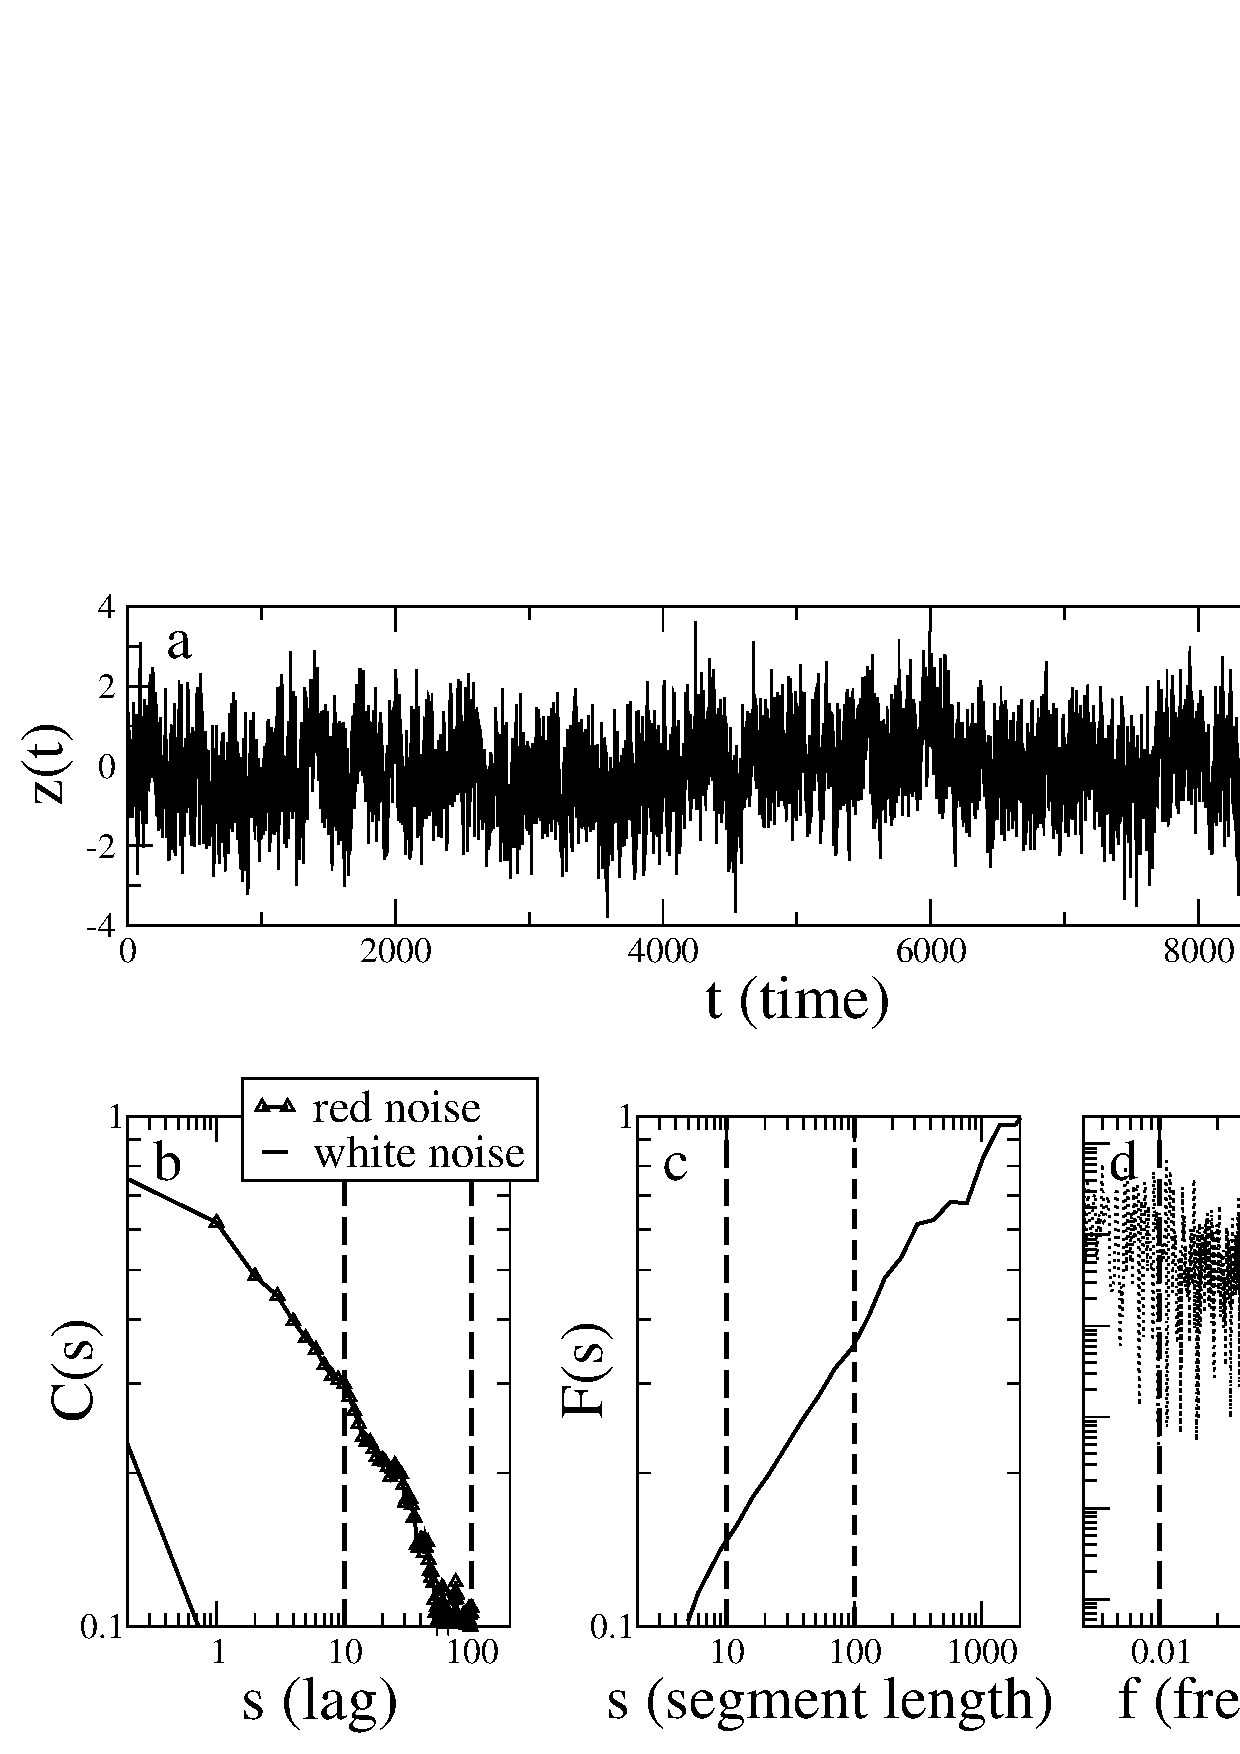
\includegraphics[width = 0.9\textwidth]{fig1_v5}
	\caption{Analysis of artificial red noise with scaling exponents measured using three different methods. Panel {\bf a}: Red noise is generated using the method shown in equation \ref{eqn:1D:simple_brownian}. Panel {\bf b}: The ACF of the red noise data is calculated for different lags and the exponent (negative slope) measured in the range $10\leq s \leq 100$ (dashed lines). We note that the ACF1 indicator ($C(1)$) is 0.84. The ACF of a white noise series is also plotted for comparison, in this case $C(s)=0$ for $s\geq 1$ and the exponent is also zero. Panel {\bf c}: DFA calculated for the data and the exponent (slope) measured in the range $10\leq s \leq 100$. Panel {\bf d}: The power spectrum of the data, and the exponent (negative slope) measured in the frequency range $10^{\m2} \leq f \leq 10^{\m1}$. \label{fig:1D:3exponents_rednoise}}
\end{figure}

\subsection{Detrended Fluctuation Analysis}
\label{subsec:1D:scaling_exponents:DFA}

Detrended Fluctuation Analysis (DFA), defined by \citet{peng1994}, is used by \citet{livina2007} as an EWS, similarly to autocorrelation. We therefore find it appropriate to draw comparisons between the two methods. Detrended Fluctuation Analysis has been applied successfully in various contexts \citep{peng1995quantification,koscielny1998,bunde2000,kantelhardt2001}. Here we describe the method used to find the DFA exponent $\alpha$.

Taking time series data $z(t)$ of length $N$, the DFA method involves calculating the cumulative sum of $z(t)$, which is called $Y$. This cumulative series is then split into $\lfloor N/s \rfloor$ non-overlapping segments $Y_{(j)},~j = 1,..., \lfloor N/s \rfloor$ and, for each segment, a `detrended' series, $\overline{Y}_{(j)}$, is found by subtracting an order-$n$ polynomial fit $p_n(Y_{(j)})$. Equations \ref{eqn:1D:DFA_method1} to \ref{eqn:1D:DFA_method2} show this process:
\begin{align}
	\label{eqn:1D:DFA_method1}
	y_i &= \sum_{k=0}^{i}x_k~~i=0,\dots,N \, ,\\
	Y_{(j)} &= \{ y_{js}, y_{js+1}, \dots, y_{(j+1)s-1}  \}~~j=0,1,\dots,\left\lfloor \frac{N}{s} \right\rfloor-1 \, ,\\
	\overline{Y}_{(j)} &= Y_{(j)} - p_n(Y_{(j)}) ~~~ j=0,1,\dots \, .
	\label{eqn:1D:DFA_method2}
\end{align}

Figure \ref{fig:1D:f2_DFAdemo} illustrates the detrending step of the DFA algorithm: the time series $z(t)$ is a pink-noise series of length 40 generated using equation \ref{eqn:1D:ColouredNoise_kasdin} with parameter $\lambda=1$ and the method shown is order-2 DFA, where a quadratic fit has been used in each segment. The detrended series $\overline{Y}$ in each segment is then the difference between $Y$ and the quadratic fit.

\begin{figure}
	\centering
	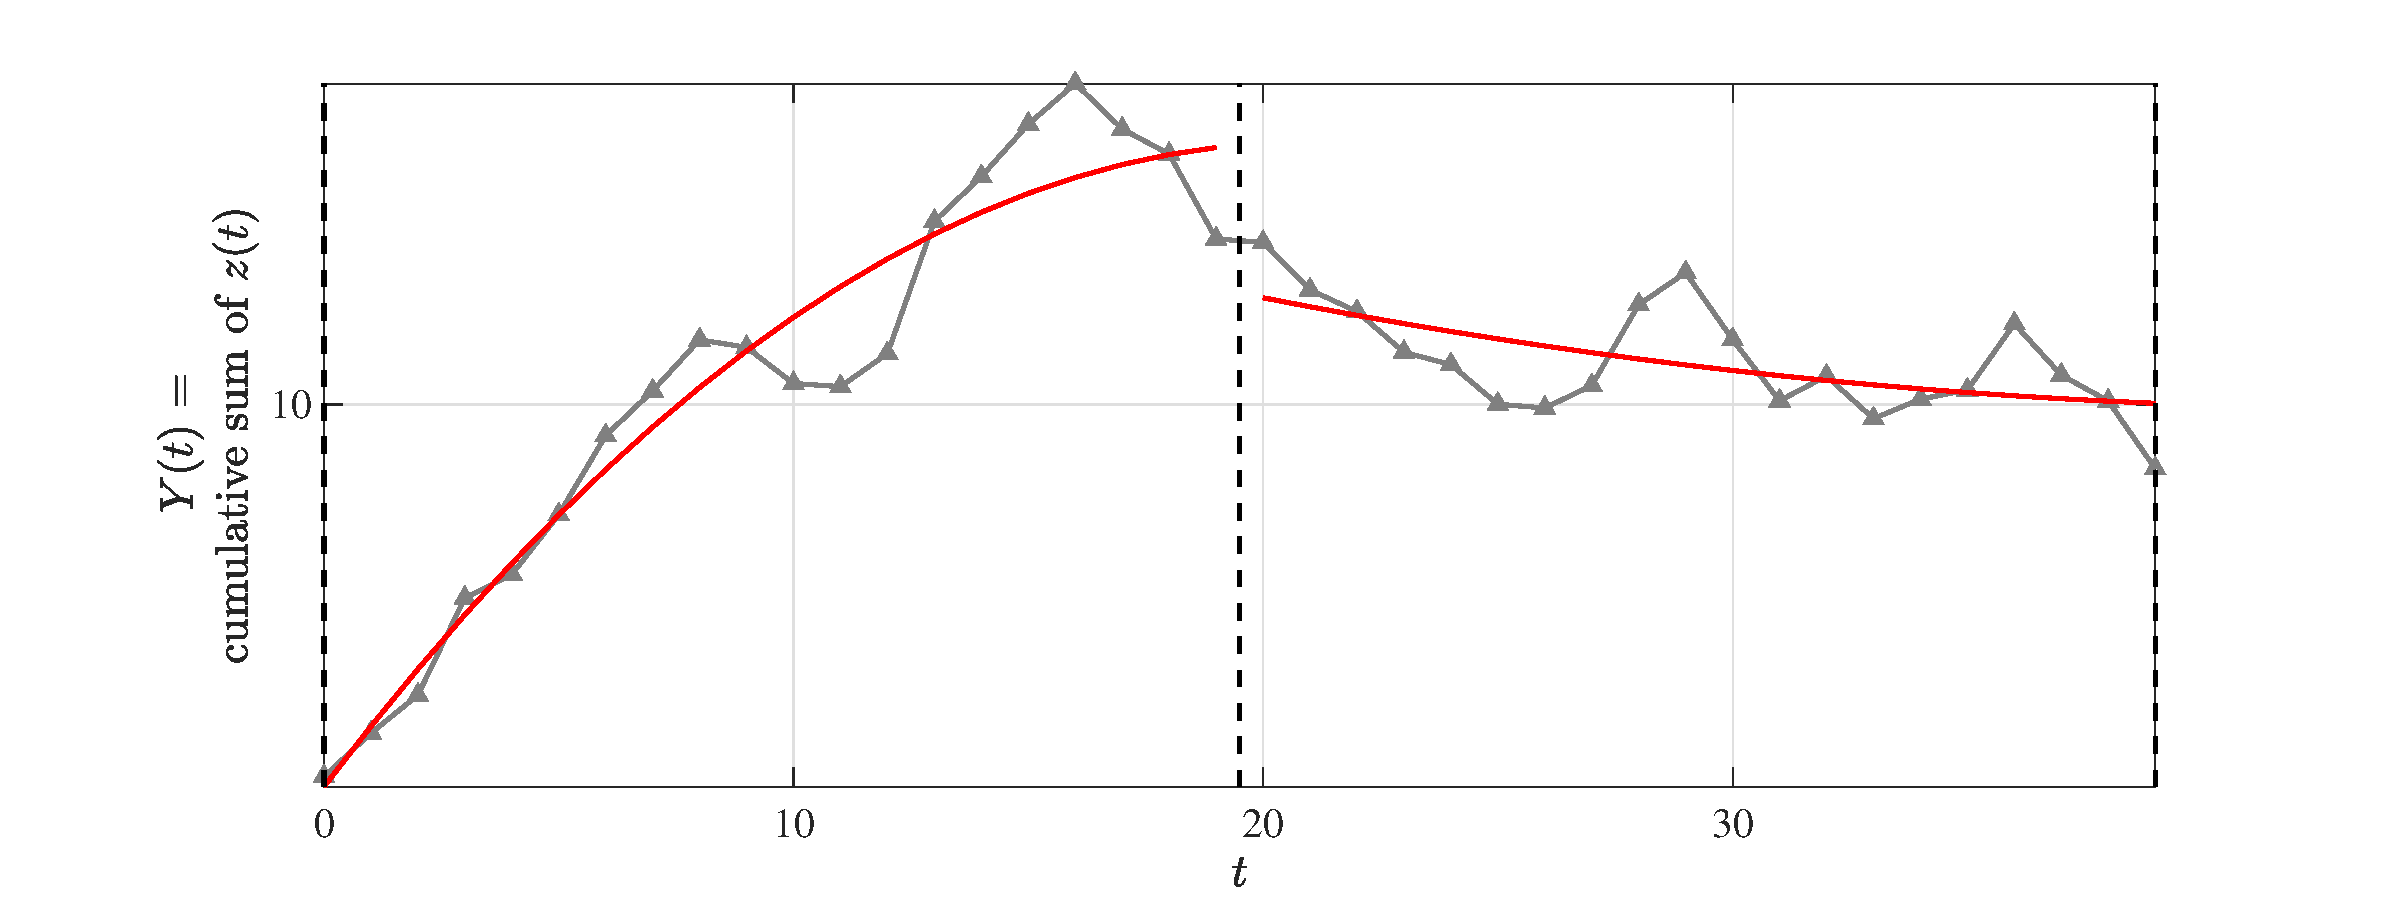
\includegraphics[width = 0.9\textwidth]{f2_DFAdemo_v2}
	\caption{The detrending step in the order-2 DFA algorithm (equation \ref{eqn:1D:DFA_method2}). The cumulative sum of a pink-noise time series $z(t)$ is shown with the quadratic best fit (red line) in each segment of length 20 (marked by dashed vertical lines). }
	\label{fig:1D:f2_DFAdemo}
\end{figure}

Given these detrended segments $\overline{Y}_{(j)}$, the equation \ref{eqn:1D:DFA} provides the $s$-dependent fluctuation coefficient $F^{(n)}(s)$:
	\begin{align}
		F^{(n)}(s) = \sqrt{ \frac{1}{\lfloor N/s \rfloor} \sum_{j=0}^{\lfloor N/s \rfloor-1} \text{Var}(\overline{Y}_{(j)})}.
		\label{eqn:1D:DFA}
	\end{align}
We define the DFA exponent in relation to the fluctuation coefficient as follows:
\begin{definition}[The DFA scaling exponent]
	\label{def:1D:DFAexponent}
	{\Red If the order-$n$ fluctuation coefficient $F^{(n)}$, as a function of segment length $s$ satisfies the power-law scaling relationship
	\begin{equation} 
		F^{(n)}(s) \sim s^{\alpha_n}, 
	\label{eqn:1D:DFA_scaling_equation} 
	\end{equation}
	then we define $\alpha_n$ as the DFA scaling exponent.}
\end{definition}
Practically, $F^{(n)}(s)$ is calculated for many values of $s$ and the value of $\alpha$ is found to be the slope of the linear best fit line to the logarithmic plot of  over $s$. Figure \ref{fig:1D:3exponents_rednoise}c shows the order-2 DFA coefficient $F^{(2)}(s)$ of the red noise time series in figure \ref{fig:1D:3exponents_rednoise}a for $s = 1,2,\dots,100$. The slope of the logarithmic plot in figure {\ref{fig:1D:3exponents_rednoise}c , obtained using a simple linear fit, is the DFA exponent $\alpha$. In this study we consistently use the order-2 DFA method, which uses a quadratic fit during the detrending step of DFA. Following the approach of \cite{livina2007}, we measure the DFA exponent in the temporal range $10\leq s \leq 100$. {\Red This range is chosen by \cite{livina2007} because, after investigation, it is found to be the range in which an increase in the DFA exponent is most sensitive to \emph{critical slowing down} which is a common feature of tipping behaviour. This is discussed further in section~\ref{subsec:1D:Exponents_as_EWS:determining_frequency_range} of this chapter where a similar investigation is carried out in the case of the power spectrum exponent.}
	
\citet{kantelhardt2001} also proposes a modified DFA method designed to provide better results with shorter time series in which long-range correlations can cause an overestimate of the exponent $\alpha$. The modified method therefore involves multiplication of the  fluctuation coefficient $F^{(n)}(s)$ by a correction function derived from $F^{(n)}(s)$ but with the segments $Y$ shuffled in a random order to destroy any long-range correlations in the data. 







\subsection{The power spectrum exponent}
\label{subsec:1D:scaling_exponents:PS}

{\Red{
Many methods of time series analysis involve transforming the series from the \emph{time domain}, in which the system state is a function of time, into the \emph{frequency domain}, in which the amount of the series lying within a frequency band is a function of frequency \citep{chatfield2016analysis}, thereby obtaining the power spectrum for the particular time series, which we define here:
}}

\begin{definition} [Power Spectrum]
	\label{def:1D:PowerSpectrum}
		{\Red{
		The Power Spectrum of a time series $x(t)$ is the Power Spectral Density (PSD) of $x(t)$ considered as a function of frequency $f$. We denote the power spectrum by $S_x(f)$. For a time series $x(t)$ with Fourier transform 
		\begin{equation}
			\label{eqn:1D:fourier_transform}
			\hat{x}(f) = \int_{\m \infty}^{\infty} x(t) e^{\m 2\pi i f t} dt,
		\end{equation}
		the power spectrum $S_x(f)$ is given by the modulus squared of the Fourier transform,
		\begin{equation}
			\label{eqn:1D:power_spectrum_def}
			S_x(f) = \left|\hat{x}(f)\right|^2\,,
		\end{equation}
		where $f\in(0,1]$ and there is symmetry about $f=1/2$. That is, $S_x(f) = S_x(1-f)$.  Alternative formulations consider the PSD as a function of angular frequency $\omega=2\pi f$.}}
\end{definition}

{\Red{
We are then able to define the power spectrum scaling exponent based on the scaling behaviour of the power spectrum as a function of frequency:
}}

\begin{definition}[The power spectrum scaling exponent]
	\label{def:1D:PSexponent}
	{\Red{If the power spectral density of a process $x(t)$, as a function of frequency $f$, satisfies the power-law scaling relationship
		\begin{equation} 
			S_x(f) \sim f^{-\beta}, 
			\label{eqn:1D:PS_scaling_relationship} 
		\end{equation}
		then we define $\beta$ as the power spectrum (PS) scaling exponent.}}
\end{definition}

{\Red{
Thus the PS scaling exponent is the negative gradient of the power spectrum $S_x(f)$ plotted on logarithmic axes, provided that the plot is linear, implying the existence of power law scaling. This view is similar to the view that the autocorrelation scaling exponent is the negative gradient of the autocorrelation $R_x$ as a function of lag $\tau$, also on logarithmic axes. 

An alternative definition of the power spectrum, or PSD, is based on the auto-correlation of the time series via the Wiener-Khinchin theorem which states that the power spectrum $S_x(f)$ is equal to the Fourier transform of the auto-correlation function \citep{chatfield2016analysis}. In this way we see that the power spectrum and the auto-correlation function are closely related, which motivates the introduction of the power spectrum scaling exponent as a tool for tipping point detection \citep{prettyman2018}. In section~\ref{sec:1D:relationships} the relationship between the DFA exponent, the ACF exponent and the power spectrum exponent is discussed further. 
}}

\begin{theorem}[The Wiener-Khinchin Theorem]
\label{thm:1D:wiener-khinchin}
	{\Red{
	For a time series $x(t)$ the auto-correlation function $R_x(\tau)$ 
	given by
	\begin{equation}
		\label{eqn:1D:W-K:auto_correlation}
		R_x(\tau) = \mathbf{E}\left[x(t)x(t+\tau)\right]
	\end{equation}
	may be expressed in terms of the power spectral density thus
	\begin{equation}
		\label{eqn:1D:wiener-khinchin1}
		R_x(\tau) = \int_{\m \infty}^{\infty} S_x(f) e^{2\pi i \tau f} df,
	\end{equation}
	which is the inverse Fourier transform \citep{chatfield2016analysis}.
	}}
\end{theorem}

{\Red{
If the terms $R$ and $S$ in equation~\ref{eqn:1D:wiener-khinchin1} satisfy the conditions of Fourier inversion, i.e. that they are absolutely integrable, then we may state the theorem as
	\begin{equation}
	\label{eqn:1D:wiener-khinchin2}
		S_x(f) = \int_{\m \infty}^{\infty} R_x(\tau) e^{\m 2\pi i \tau f} d\tau = \hat{R}_x(f).
	\end{equation}
This Fourier transform formulation is often used as the definition of the power spectrum \citep{ricker2012}, and is similarly expressed in the case of a discrete-time process $x(n)$ as follows:
	\begin{equation}
	\label{eqn:1D:wiener-khinchin:discrete}
		S_x(f) = \sum_{k=\m \infty}^{\infty} R_x(k) e^{\m 2\pi i f k},
	\end{equation}
where the discrete time autocorrelation is given by
	\begin{equation}
	\label{eqn:1D:autocorellation:discrete}
		R_x(k) = \mathbf{E}\left[x(n) x(n-k)\right].
	\end{equation}

This discrete time formulation, however, does not provide a useful method for the calculation of the power spectrum of a process given a finite time series, due to the infinite sum, even if the sample ACF is used to approximate $R_x$. Instead, in the experiments presented in this thesis, the power spectrum as defined by the Fourier transform (definition~\ref{def:1D:PowerSpectrum}) is approximated directly using the fast Fourier transform (FFT) as implemented in Matlab by \cite{frigo2005}. This straight-forward approximation of the power spectrum using a discrete-time FFT is known as a \emph{periodogram} \citep{welch1967, oppenheim1999}.
}}

\begin{definition}[Periodogram]
\label{def:1D:periodogram}
	{\Red{The periodogram $\hat{P}(f')$ of a time series $x_n$ of length $N$, as used throughout this thesis, is defined by the equation 
	\begin{equation}
		\label{eqn:1D:periodogram_def}
		\hat{P}(f') = \frac{1}{N}\left|\sum_{n=0}^{N-1}x_n e^{\m 2\pi i f' n}\right|^2, ~~~~~ f' = 0, \frac{1}{N},\frac{2}{N}, ..., 1,
	\end{equation}
	where $f'$ is a discrete variable equivalent to the frequency $f$ in the power spectrum (definition~\ref{def:1D:PowerSpectrum}). The summation term is the fast Fourier transform as implemented in Matlab \citep{frigo1998,frigo2005}. In this thesis, for the purposes of using the periodogram as a tool for tipping point detection, we consider only the one-sided periodogram, that is, the periodogram $\hat{P}(f')$ for the frequency range $f'\in (0,1/2]$, and so the calculation is performed only for the values
	\begin{equation}
		f' = \frac{1}{N},\frac{2}{N}, ..., \frac{1}{N}\left\lfloor \frac{N}{2} \right\rfloor,
	\end{equation}
	since the periodogram, as defined here, is symmetric about $f'=1/2$ \citep{fulop2006}.}}
\end{definition}


{\Red{
Having obtained the periodogram from a given discrete time series, an estimation of the power spectrum scaling exponent $\beta$ (equation~\ref{eqn:1D:PS_scaling_relationship}) is found by measuring the negative gradient of the periodogram on logarithmic axes, assuming that a power law scaling relationship exists. This is done by fitting a linear function to the logarithmic plot in a predetermined range of frequencies. When the power spectrum scaling exponent $\beta$ is estimated in this way throughout this thesis, in which $\beta$ is used as an early warning indicator, we typically use the frequency range $10^{\m2}\leq f \leq 10^{\m1}$ unless otherwise stated. This corresponds to the time scale range $10\leq s \leq 100$ used in the calculation of the DFA exponent \citep{livina2007} as discussed in section~\ref{subsec:1D:scaling_exponents:DFA} but the precise reason for this choice of frequency range is motivated by the phenomenon of \emph{critical slowing down} and will be discussed further in section~\ref{subsec:1D:Exponents_as_EWS:determining_frequency_range}. 

{\label{pageref:1D:logbinning} We note that the frequencies used in the calculation of the periodogram in equation~\ref{eqn:1D:power_spectrum_def} occur linearly between 0 and 1 and therefore the periodogram, when plotted on logarithmic axes}, has a greater concentration of points in the higher frequencies. For example, when $N=10^4$ there are 91 values of $f'$ for which $\m3\leq\log f'\leq\m2$ but 901 values of $f'$ for which $\m2\leq\log f'\leq\m1$, although both ranges are of equal length on the logarithmic scale. When a linear function is fitted to the periodogram using a least squares optimisation in order to calculate the gradient, more weight will therefore be given to the gradient described by the points at the higher end of the frequency range. In order to overcome this effect a more linear distribution of points is first obtained by binning the frequencies logarithmically, before a linear fit is attempted. The periodogram window, defined by $10^{\m2}\leq f' \leq 10^{\m1}$ (or whichever lower and upper bounds may be used), is split into a number of subwindows of equal length on the logarithmic scale such that the first subwindow contains $m$ points where $m\geq 2$. All other subwindows after the first are then divided into $m$ partitions and the new series of \emph{binned periodogram} data $P_B(f)$ is defined as the means of the periodogram points $\hat{P}(f')$ in each partition. The new series of frequencies $f$ are the midpoints (on the logarithmic scale) of the partitions. 
}}

\begin{figure}
	\centering
	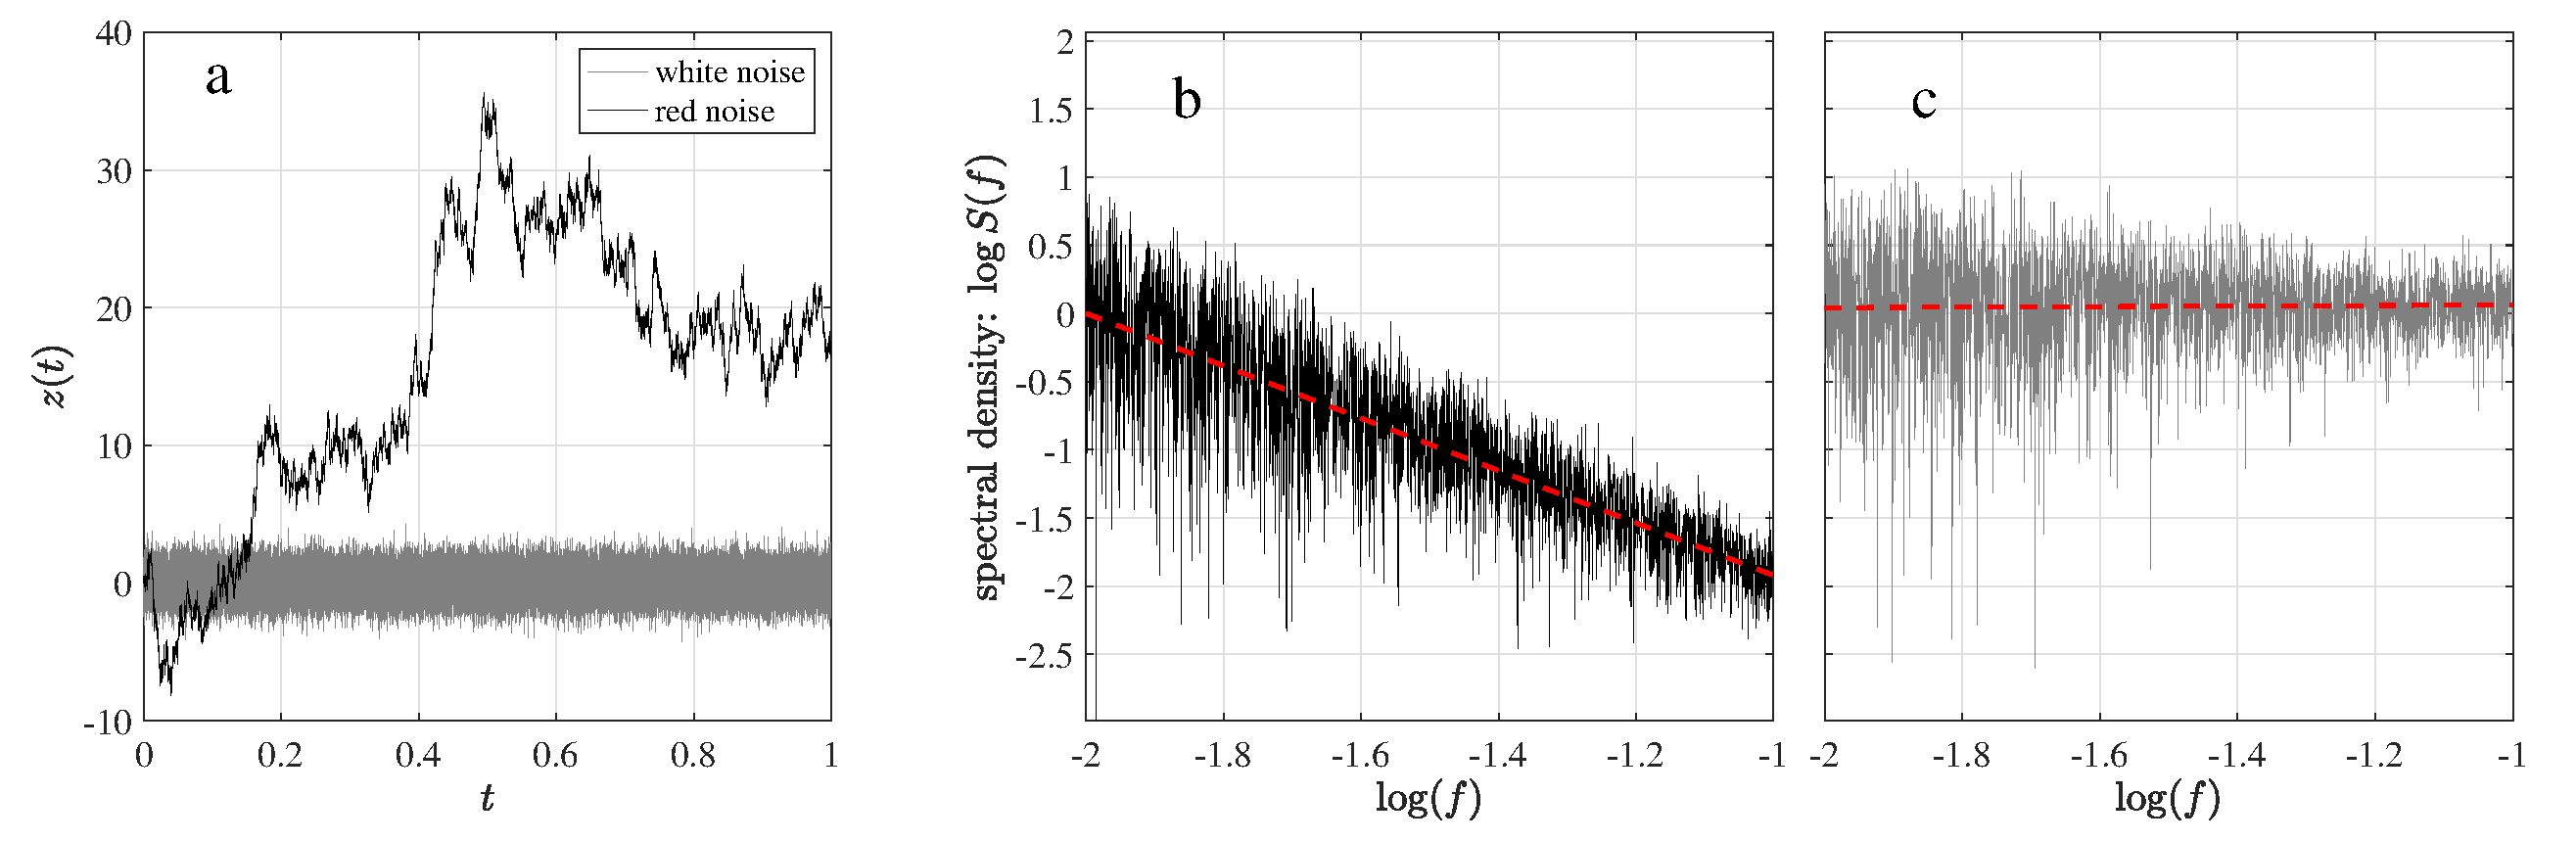
\includegraphics[width = 0.9\textwidth]{PS_scaling_calculation}
	\caption{\Red PS exponent estimation for red noise and white noise. Panel {\bf a}: A simple Gaussian discrete white noise series and a random walk (red noise, see equation~\ref{eqn:1D:simple_brownian}) are generated, both of length $10^5$. Panels {\bf b} and {\bf c}: For the red noise and white noise series respectively, the periodogram is plotted on a log-log scale in the frequency range $\m2\leq\log f\leq\m1$ and a linear best fit (dashed red line) is used to calculate the gradient. We find the PS exponents to be $1.998$ and $0.000$ for red and white noise respectively.}
	\label{fig:1D:PS_scaling_calculation}
\end{figure}

{\Red{
In figure~\ref{fig:1D:PS_scaling_calculation} the PS exponent is calculated for a red noise series and a white noise series (both of length $10^5$) using the linear best fit to estimate the negative gradient of the periodogram. In this figure the periodogram is plotted after the logarithmic binning step. By comparison, the demonstration of the same method in figure~\ref{fig:1D:3exponents_rednoise}d (page~\pageref{fig:1D:3exponents_rednoise}) does not use logarithmic binning, we note the higher variability in the higher frequencies.

Other methods exist to estimate the power spectrum, such as Welch's method \citep{welch1967} and the multi-taper method \citep{thomson1982}, both of which are based on the periodogram and are designed to reduce noise. Since, in this thesis, we are not concerned with identifying specific features of the power spectrum, only measuring the gradient to provide an estimate of the scaling exponent $\beta$, the ordinary periodogram, after logarithmic binning, is usually sufficient. If, however, it is necessary to determine whether power law scaling exists, it may be useful to reduce the noise using Welch's method in order to more easily determine visually whether power spectrum describes a straight line. Other methods of power spectrum estimation are often developed for specific applications in engineering \citep{bingham1967}.

}}



\section{Relationships between scaling exponents}
\label{sec:1D:relationships}

\subsection{White noise and red noise}
\label{subsec:1D:relationships:white_and_red_noise}
{\Red
	
In chapter~\ref{chap:intro} two examples of a noisy signal are introduced: discrete Gaussian white noise, in which each term is sampled from an independent, identical Gaussian distribution; and the discrete random walk which is the cumulative sum of Gaussian white noise. Now that we have defined the power spectrum (definition~\ref{def:1D:PowerSpectrum}) we are able to properly define the term \emph{white noise}, which is not necessarily Gaussian:

\begin{definition}[White noise]
	\label{def:1D:whitenoise}
	A white noise process $w_t$ is a random signal with equal power spectral density at all frequencies, that is, the power spectrum of the process is a constant:
	\begin{equation}
		\label{eqn:1D:white_noise_def}
		S_w(f)=\left|\hat{w}(f)\right|^2 = \left|\int_{\m \infty}^{\infty} w_t e^{\m 2\pi i f t} dt\right|^2 = C\,,
	\end{equation}
	for positive constant $C$ \citep{robinson2012introduction}.
\end{definition}

Since this power spectrum $S_w(f)$ follows the power law scaling relationship
\begin{equation}
	S_w(f) = C = f^0 C\,,
\end{equation}
we say it has PS exponent $\beta = 0$. Although we note that if a discrete time series is found to have a PS exponent of zero using the periodogram method presented in section~\ref{subsec:1D:scaling_exponents:PS}, this does not necessarily imply that the process is white noise.

A corollary of the definitions of a white noise series is that
	\begin{equation}
	\label{eqn:1D:white_noise:corollary}
		\left|\hat{w}(f)\right|^2 = C ~~\Rightarrow~~ \hat{w}(f) = \sqrt{C}e^{i\theta f}\,,
	\end{equation}
for some $\theta\in [\m\pi, \pi]$. In this thesis only Gaussian white noise is considered, in which case the distribution of the values of $w_t$ will be Gaussian, although many other distributions of values could also result in a constant power spectrum. In computational examples and experiments throughout this thesis, whenever a white noise series is required, a discrete-time series of length $N$ is generated simply by using the Matlab random number generator function $\texttt{randn(1,N)}$, which returns $N$ independent identically distributed values sampled from a normal distribution with mean zero and variance $\sigma^2=1$. 

We are then able to show that the Gaussian noise process $\eta_t$, as we have been using it, actually is a white noise process according to the definition. From the simple observation that the expected value of the product of two independent random variables with zero mean is zero, we can express the autocorrelation function of the Gaussian white noise as
\begin{equation}
	\label{eqn:1D:white_noise:autocorellation}
	R_\eta(k) = \mathbf{E}\left[\eta(n) \eta(n-k)\right] 
	= \left\{ \begin{array}{lr}
	0 , & k\neq 0 \\
	1 , & k=0
	\end{array} \right. ,
\end{equation}
where, in this case, the variance of the white noise terms $\eta$ is 1. This result is similar in appearance to the continuous-time case which can be derived from the Wiener-Khinchin theorem. The theorem defines the autocorrelation $R_x$ of process $x$ as the inverse Fourier transform of the power spectrum. Since the power spectrum of white noise is a constant, we have
\begin{equation}
	\label{eqn:1D:autocorrrelation_dirac}
	R_eta(\tau) = \int_{\m \infty}^\infty S_\eta(f)e^{2\pi i \tau f}df = C\int_{\m \infty}^\infty e^{2\pi i \tau f}df = C\delta(\tau)\,,
\end{equation} 
since the inverse Fourier transform of the constant function $S(f)=1$ is the Dirac delta function \citep{kammler2007fourier} which has an infinitely large spike at $\tau =0$. We note that, clearly, there does not exist power law scaling for the function $R_\eta$. The discrete-time formulation in equation~\ref{eqn:1D:white_noise:autocorellation} allows us, using the discrete-time Wiener-Khinchin theorem (equation~\ref{eqn:1D:wiener-khinchin:discrete}), to calculate the power spectrum as follows:
\begin{equation}
\label{eqn:1D:PSofWhiteNoise}
	S_\eta(f) = \sum_{k=\m \infty}^{\infty} R_\eta(k) e^{\m 2\pi i f k} = R_\eta(0) e^{0} = 1\,.
\end{equation}
The power spectrum of the Gaussian noise is thus constant and is therefore white noise according to definition~\ref{def:1D:whitenoise}. We are also able to compute the power spectrum of the random walk series, simply the cumulative sum of a Gaussian white noise series. This is the discrete time analogue of the continuous Wiener process, which is defined as a process $W_t$ such that the derivative is a Gaussian process:
\begin{equation}
	\label{eqn:1D:Wiener_process}
	\frac{d}{dt}W_t = \eta_t.
\end{equation}
Or, conversely, as the integral of a Gaussian process. Using this definition we may compute the power spectrum of a Wiener process using the Fourier transform identity that if $\hat{x}(f)$ is the Fourier transform of $x(t)$, then 
\begin{equation}
	\widehat{\frac{d}{dt}x(t)} = (2\pi i f)\hat{x}(f).
\end{equation} 
For the Wiener process this identity becomes
\begin{equation}
	\widehat{\frac{d}{dt}W_t} = (2\pi i f)\hat{W}_t\,,
\end{equation} 
or
\begin{equation}
	(2\pi i f)\hat{W}_t = \hat{\eta}_t = e^{i\theta f}\,,
\end{equation} 
for some $f\in[\m\pi, \pi]$, as shown in equation~\ref{eqn:1D:white_noise:corollary}. Therefore the power spectrum is given by
\begin{equation}
	\label{eqn:1D:rednoise_scalingfactor}
	S_W(f) = \left|\hat{W}_t\right|^2 = \left|\frac{e^{i\theta f}}{2\pi i f}\right|^2 = \frac{1}{4\pi^2}f^{\m 2}\,,
\end{equation} 
and so the Wiener process has power spectrum scaling exponent $\beta = 2$. While a stochastic process with a constant power spectrum is known as \emph{white noise}, and this has PS exponent $\beta =0$, the random walk, or Wiener process, with a PS scaling exponent of $\beta = 2$ is known as \emph{red noise}. Stochastic processes with PS scaling exponent in the range $0<\beta<2$ are known as \emph{pink noise} (given that a power law scaling relationship exists). It is often a ``reddening'' of noise, the increase in the PS exponent from 0 to 2, that we will try to detect when investigating tipping points. Recalling the changing shape of the generalised potential ``well'' in the pitchfork bifurcation example (see figure~\ref{fig:intro:ChangingPotential}, page~\pageref{fig:intro:ChangingPotential}), we are able to understand intuitively why such reddening of noise, a building up of memory in the system, may occur. When the the generalised potential is a steep ``well'' shape we expect that any small perturbation from the stable state will return quickly to the mean. However, as the shape becomes shallower, small perturbations may continue in the direction away from the mean, resembling a random walk. This increased return time to the stable state is known as \emph{critical slowing down} \cite{scheffer2009critical} and is a typical feature of tipping points in dynamical systems, not only the pitchfork bifurcation. 

}

\subsubsection{The relationship between $\beta$ and $\gamma$}
\label{subsec:1D:relationships:beta_and_gamma}
{\Red
	
The Wiener-Khinchin theorem (theorem~\ref{thm:1D:wiener-khinchin}) states that there is a relationship between the autocorrelation $R_x$ and the power spectrum $S_x$ of a process $x$ in that the two are a Fourier transform pair, that is
	\begin{equation}
		R_x(\tau) = \int_{\m \infty}^\infty S_x(f)e^{2\pi i \tau f} df\,.
	\end{equation}
Indeed, this relation is often used to define the power spectrum \citep{chatfield2016analysis}. We now use this theorem to investigate the relationship between the ACF scaling exponent $\gamma$ and the PS scaling exponent $\beta$. Say the process $x$ has a power spectrum scaling exponent $\beta$, then by definition we have $S_x(cf) = c^{\m\beta}S_x(f)$
for some constant $c$, or
	\begin{equation}
		S_x(f) = c^{\beta}S_x(cf)\,.
	\end{equation}
Now we attempt to find if power law scaling exists for the autocorrelation function by calculating $R_x(c\tau)$ as follows:
	\begin{equation}
	\begin{split}
		R_x(c\tau) &= \int_{\m \infty}^\infty S_x(f)e^{2\pi i c\tau f} df\\
		&= \int_{\m \infty}^\infty c^{\beta}S_x(cf)e^{2\pi i c\tau f} df\,.
	\end{split}
	\end{equation}
Using the substitution $g = cf$, and so $df/dg = 1/c$, we obtain
	\begin{equation}
	\begin{split}
	R_x(c\tau) &= \int_{\m \infty}^\infty c^{\beta}S_x(g)e^{2\pi i \tau g} \frac{1}{c} dg\\
	&= c^{\beta\m 1}\int_{\m \infty}^\infty S_x(g)e^{2\pi i \tau g} dg\\
	&= c^{\m(1\m\beta)}R_x(\tau)\,.
	\end{split}
	\end{equation}
Then we see that the process $x$ has an ACF scaling exponent $\gamma = 1-\beta$, thus giving a relationship between the PS and ACF exponents:
	\begin{equation}
	\label{eqn:1D:beta-gamma_linear_relation}
		\beta = 1-\gamma\,,
	\end{equation}
where scaling exists in both the ACF and the power spectrum. As we have noted above (equation~\ref{eqn:1D:autocorrrelation_dirac}) there is not strictly power law scaling in the autocorrelation function of white noise, even though there is scaling in the power spectrum. The autocorrelation of the ``red noise'' Wiener process would be given by the Wiener-Khinchin theorem as
	\begin{equation}
		\begin{split}
		R_W(\tau) &= \int_{\m \infty}^\infty S_W(f)e^{2\pi i \tau f} df\,,\\
		&= \int_{\m \infty}^\infty \frac{1}{|2\pi f|^2}e^{2\pi i \tau f} df\,,
		\end{split}
	\end{equation}
but it is not possible to evaluate the integral because of the singularity at $f=0$ \citep{kammler2007fourier}. Taking a different approach, we look to the definition of the \emph{normalised} autocorrelation
	\begin{equation}
		R_{W_t}(\tau) = \frac{1}{\sigma_{W_t} \sigma_{W_{t+\tau}}} \mathbf{E}\left[W_t W_{t+\tau}\right].
	\end{equation}
where $\sigma_{W_t}^2$ is the variance of the Wiener process $W$ at time $t$. The properties of the Wiener process lead to the expression
	\begin{equation}
		R_{W_t}(\tau) = \sqrt{\frac{t}{t+\tau}}, 
	\end{equation}
\citep{stark2002probability} where the dependence on $t$ comes from the fact that the Wiener process is non-stationary. Clearly, for some fixed value $t$, this is not a power-law scaling relationship in $R_{W_t}$ as a function of $\tau$. 

We have shown here that $\beta$ and $\gamma$ are related linearly as $\beta = 1-\gamma$, and also that in the case of a white noise process and also the Wiener process, the autocorrelation function does not exhibit power-law scaling and so $\gamma$ does not exist. Table~\ref{tab:1D:exponent_relationships} shows the results of attempting to numerically estimate the scaling exponents given a finite, discrete time series. Two processes are used to generate the time series: a Gaussian white noise process where each term is sampled independently from a Gaussian distribution; and a random walk which is simply the cumulative sum of a Gaussian white noise series. The scaling exponents are estimated using the methods described in section~\ref{sec:1D:scaling_exponents}, where the range of lags in which $\gamma$ is estimated by linear fit is $10\leq\tau\leq100$ and the range of frequencies in which $\beta$ is estimated is $10^{\m2}\leq f \leq 10^{\m1}$. In this case the range is arbitrary since, if power law scaling exists, then it does not matter in which range the exponent is measured because the (logarithmic) power spectrum is a straight line over the whole domain $0\leq f \leq 1/2$. However, in other contexts the range does have a significant impact on the method: the reasons why this particular range $10^{\m2}\leq f \leq 10^{\m1}$ is used consistently throughout this thesis will be discussed in section~\ref{subsec:1D:Exponents_as_EWS:determining_frequency_range}. The values of $\alpha$, $\beta$, $\gamma$ and the lag-1 ACF presented in table~\ref{tab:1D:exponent_relationships} are the mean values over 1000 trials of the experiment using, in each experiment, a Gaussian white noise time series and a random walk time series of length $10^6$.

We note that the PS exponent behaves as predicted with a value $\beta=0$ (constant power spectrum) for white noise and $\beta=2$ (power spectrum scales as $f^{\m 2}$) for the random walk. However, the linear relation with the ACF exponent, $\gamma = 1-\beta$, which is shown to exist based on the definitions, does not hold. This is because the relationship is shown to exist only when power-law scaling is assumed to exist in both the power spectrum and the ACF and, as we have shown, the ACF does not exhibit power-law scaling for Gaussian white noise nor the random walk. We are able to note that the value in the case of white noise, $\gamma=0$, is expected from the analytical calculations, so long as the range of lags in which the exponent is estimated does not include $\tau=0$ (which is where the delta function spike occurs). Since the ACF for the random walk is a function of $\tau$ which is not a power law, it describes a curve, rather than a straight line, in the logarithmic plot and the local gradient will depend on the range of lags used. In section~\ref{subsec:1D:Exponents_as_EWS:nopowerlawsacaling} we will discuss the relevance of estimating scaling exponents in series for which power-law scaling does not exist. 

}

\subsubsection{The relationship between $\alpha$ and $\beta$}
\label{subsec:1D:relationships:alpha_and_beta}
\begin{table}
	\centering
	\begin{tabular}{l  r r r r }
		\toprule
		& \multicolumn{4}{c}{Exponent} \\
		\cmidrule(r){2-5}
		Signal    & DFA ($\alpha$) & PS ($\beta$) & ACF ($\gamma$) & lag-1 ACF  \\
		\midrule
		{White Noise} & 0.510 & 0.0110&-0.0163 & -0.00371 \\
		{Random Walk}   & 1.50  & 2.04 & 0.473  &  0.993\\
		%{Red 63}& 1.48 & 1.92 & 0.565  &  0.990\\
		\bottomrule
	\end{tabular}
	\caption{Mean values of three scaling indicators, and lag-1 ACF, applied to different noise signals.
	\label{tab:1D:exponent_relationships}}
\end{table}

The three scaling exponents defined in section \ref{sec:1D:scaling_exponents} are illustrated in figure \ref{fig:1D:3exponents_rednoise} where they are applied to a red noise series. The red noise, in this case, is a random walk, the simple cumulative sum of a white noise series (see equation~\ref{eqn:1D:simple_brownian}). Since all three methods give a measure of scaling, there is a relationship between them. 

Table \ref{tab:1D:exponent_relationships} shows the results of calculating the value of each exponent for both a white noise series and a random walk. In each case the value given is the mean value of the exponent calculated for $1000$ series of length $10^6$.
   
The values of $\alpha$ and $\beta$ in table \ref{tab:1D:exponent_relationships} confirm the linear relationship
	\begin{equation} 
		\alpha = \frac{1+\beta}{2} \label{eqn:1D:alphabetaExponentRelationships} 
	\end{equation}
noted by \citet{kantelhardt2001} to apply generally to these exponents. We have shown already (equation~\ref{eqn:1D:beta-gamma_linear_relation}) that the ACF scaling exponent $\gamma$ is also linearly related to $\beta$ as $\beta=1-\gamma$ where $\gamma$ and $\beta$ exist (that is, where a power law scaling relation exists for the ACF and the power spectrum). All three exponents therefore have the relationship
	\begin{equation}
		\beta = 2\alpha-1 = 1-\gamma\,,
	\end{equation} 
as noted by \cite{makse1996}. The relationship between $\alpha$ and $\beta$ is also noted by \citet{heneghan2000} to exist only for long-range correlated noise series, although here we have used only uncorrelated white noise and the random walk as a single example of a correlated series. In a further experiment, the DFA and PS exponents are calculated for multiple noise series with spectral densities between white and red noise. In this experiment we use two alternate methods of generating a noise series. The first method is the an auto-regressive model of order 1, or AR(1) model, given by the equation 
	\begin{equation}
		z_{n} = \mu z_{n-1}+\eta_{n}
	\label{eqn:1D:AR1_model}
	\end{equation}
where $\eta$ is white noise. This noise signal we refer to as being "short-range correlated", since the correlation is defined by parametrising the lag-1 autocorrelation by the single parameter $\mu$. We use $\mu=0, 0.005, \dots, 1$ to generate 200 short-range correlated noise series of length $10^6$ using this AR(1) model. 

The second method of generating a noise signal, which we call "long-range correlated", is to use an AR(63) model, described by \citet{kasdin1995}, since this is implemented in Matlab's DSP system toolbox. Simply, the method uses an auto-regressive model of order 63 with a zero-mean white noise signal $\eta(t)$:
	\begin{equation}
		\sum_{i=0}^{63} a_i z(t-i) = \eta(t),
	\label{eqn:1D:ColouredNoise_kasdin}
	\end{equation}
where the AR coefficients $a_i$ are calculated recursively by
	\begin{equation}
		a_0 = 1 ~~~~ a_k = \left(k-1-\frac{\lambda}{2}\right)\frac{a_{k-1}}{k} ~~~ k=1,2,\dots\, .
	\end{equation}
We note that where $\lambda=2$ the coefficients are 
	\begin{equation}
		a_0 = 1 ~,~ a_1 = -1 ~,~~ a_i = 0 ~~\forall i\geq2\,,
	\end{equation}
which results in the same process as defined by the AR(1) model for $\mu=1$, that is, a random walk. {\Red However, for other values of the parameter $\lambda$ the two methods differ. A value $\lambda=1$ does not correspond, for example, to the AR(1) process with $\mu=1/2$, in the former case parameters are given by
	\begin{equation}
		a_0 = 1 ~,~ a_1 = -\frac{1}{2} ~,~ a_2 = -\frac{1}{8} ~,~ a_3 = \frac{\m 1}{16}~,~ a_4 = \frac{\m 5}{128}~,~\dots\,,
	\end{equation}
giving us the AR(63) process
	\begin{equation}
		z_{t+1} = \frac{1}{2}z_{t} + \frac{1}{8}z_{t-1} + \frac{1}{16}z_{t-2} + \frac{5}{128}z_{t-3} + \dots + \eta_{t+1}\,,
	\end{equation}
as opposed to the AR(1) process
	\begin{equation}
		z_{t+1} = \frac{1}{2}z_{t} + \eta_{t+1}\,.
	\end{equation}
The additional coefficients $a_2$, $a_3$, etc., not present in the AR(1) model, introduce additional long-range correlations into the process. }
For the experiment we generate 200 series by this method, with a range of $\lambda$ between $0$ and $2$.

\begin{figure}
	\centering
	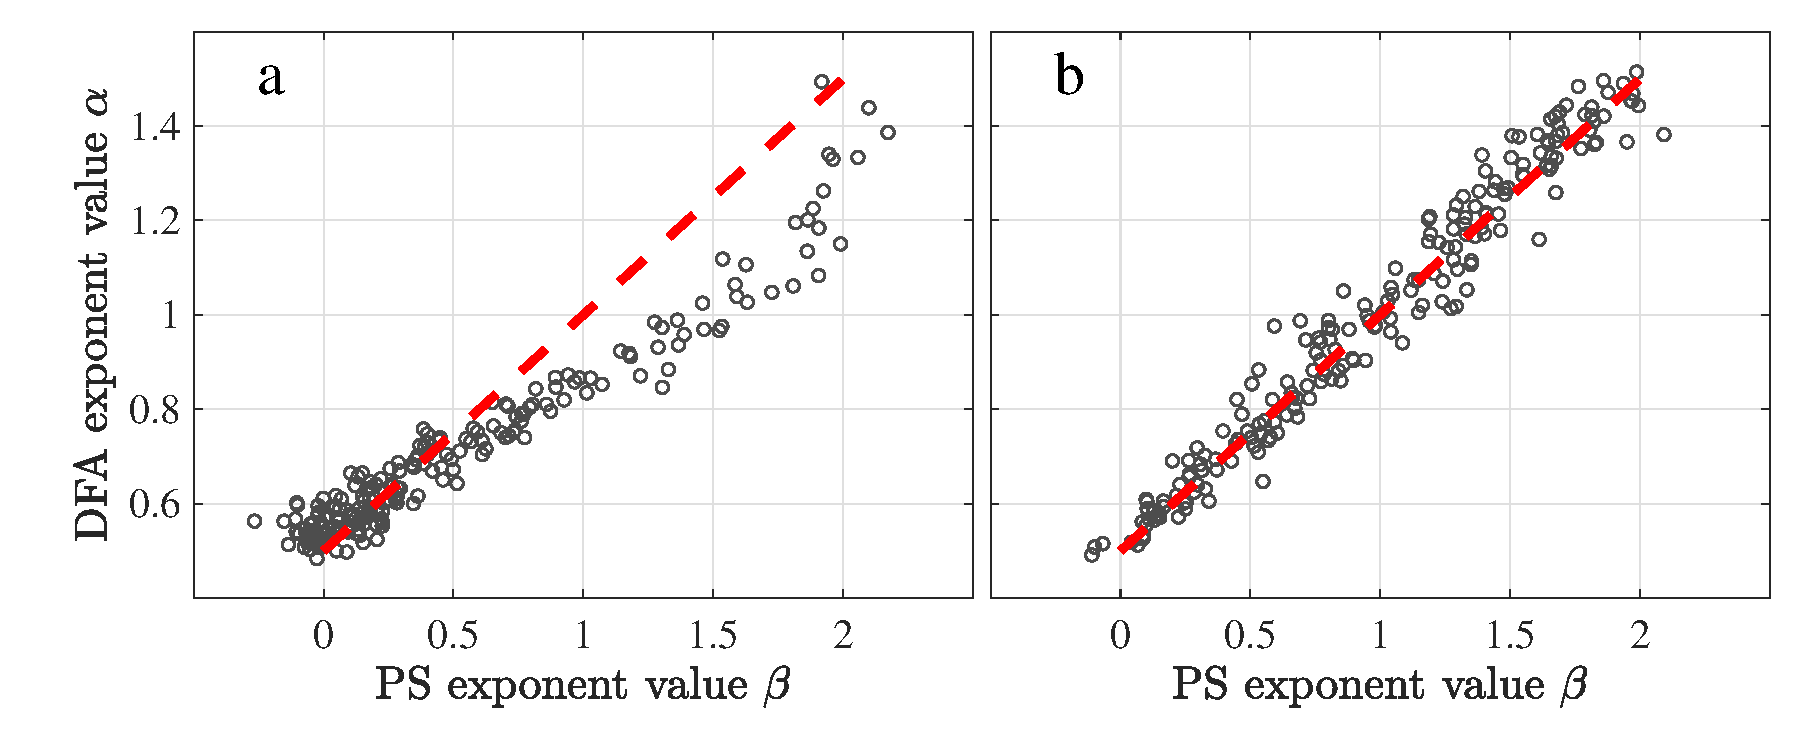
\includegraphics[width=0.9\textwidth]{f3_ExponentRelationships_v2}
	\caption{DFA exponent $\alpha$ plotted against the PS exponent $\beta$ for short-range correlated (panel {\bf a}) and long-range correlated (panel {\bf b}) noise series of length $10^4$ with varying correlation parameters. The result for each noise series is represented by one marker, the expected linear relationship is shown in red, see equation \ref{eqn:1D:alphabetaExponentRelationships}.}
	\label{fig:1D:ExponentRelationships}
\end{figure}

The DFA and PS exponents are calculated for each of the 200 short-range correlated (AR(1)) series and each of the 200 long-range correlated (AR(63)) series. The results are shown in figure \ref{fig:1D:ExponentRelationships}. We see that although the linear relationship given by equation \ref{eqn:1D:alphabetaExponentRelationships} is confirmed by the long-range correlated noise (panel {\bf b}), but not exactly by the short-range (panel {\bf a}).

An alternative method of producing long range correlated noise was to transform the power spectrum of white noise in the frequency domain, thus changing the PS exponent $\beta$ \citep{makse1996}. That is, we first sample from a Gaussian distribution to approximate white noise, $X(t)$, we then take the fast Fourier transform of this white noise series (denoted $\hat{X}(f)$) and then transform this by
	\begin{equation} 
	\label{eqn:1D:creatingColouredNoise}
		\hat{Y}(f) := \hat{X}(f)\sqrt{f^{-\beta}}.
	\end{equation}
Finally, we use the inverse fast Fourier transform to obtain the series $Y(t)$ in the time domain, which has power spectrum $S(f)$ proportional to $f^{-\beta}$. The result when using this method of noise generation is quantitatively and qualitatively similar to the result when using the AR(63) model (figure \ref{fig:1D:ExponentRelationships} panel {\bf b}): the DFA and PS exponents are strongly correlated and obey the linear relationship $\alpha = (1+\beta)/2$.


\citet{kantelhardt2001} notes that a direct calculation of the ACF scaling exponent $\gamma$ is often unsuitable due to noise and underlying trends. The DFA method is therefore introduced as an indirect measure of the exponent. In our own implementations of the two methods, the ACF exponent is less reliable. Figure \ref{fig:1D:ACFDFAreliability} illustrates this in the case that both methods are applied to noise series generated using the AR(63) model \citep{kasdin1995} with varying values of the parameter $\lambda$. Fifty noise series of length $10^4$ are generated for each value $\lambda = 0, 0.02, 0.04, ..., 1$, at each value $\lambda$ the scaling exponent is calculated for each of the 50 series and the standard deviation over these 50 exponents is found. We see that the DFA exponent is consistent in that the standard deviation of its value is low, and indeed the standard deviation is, itself, consistently low. The standard deviation is much larger in the ACF exponent, although the exponents have similar mean values (between 0 and 1).





\begin{figure}
	\centering
	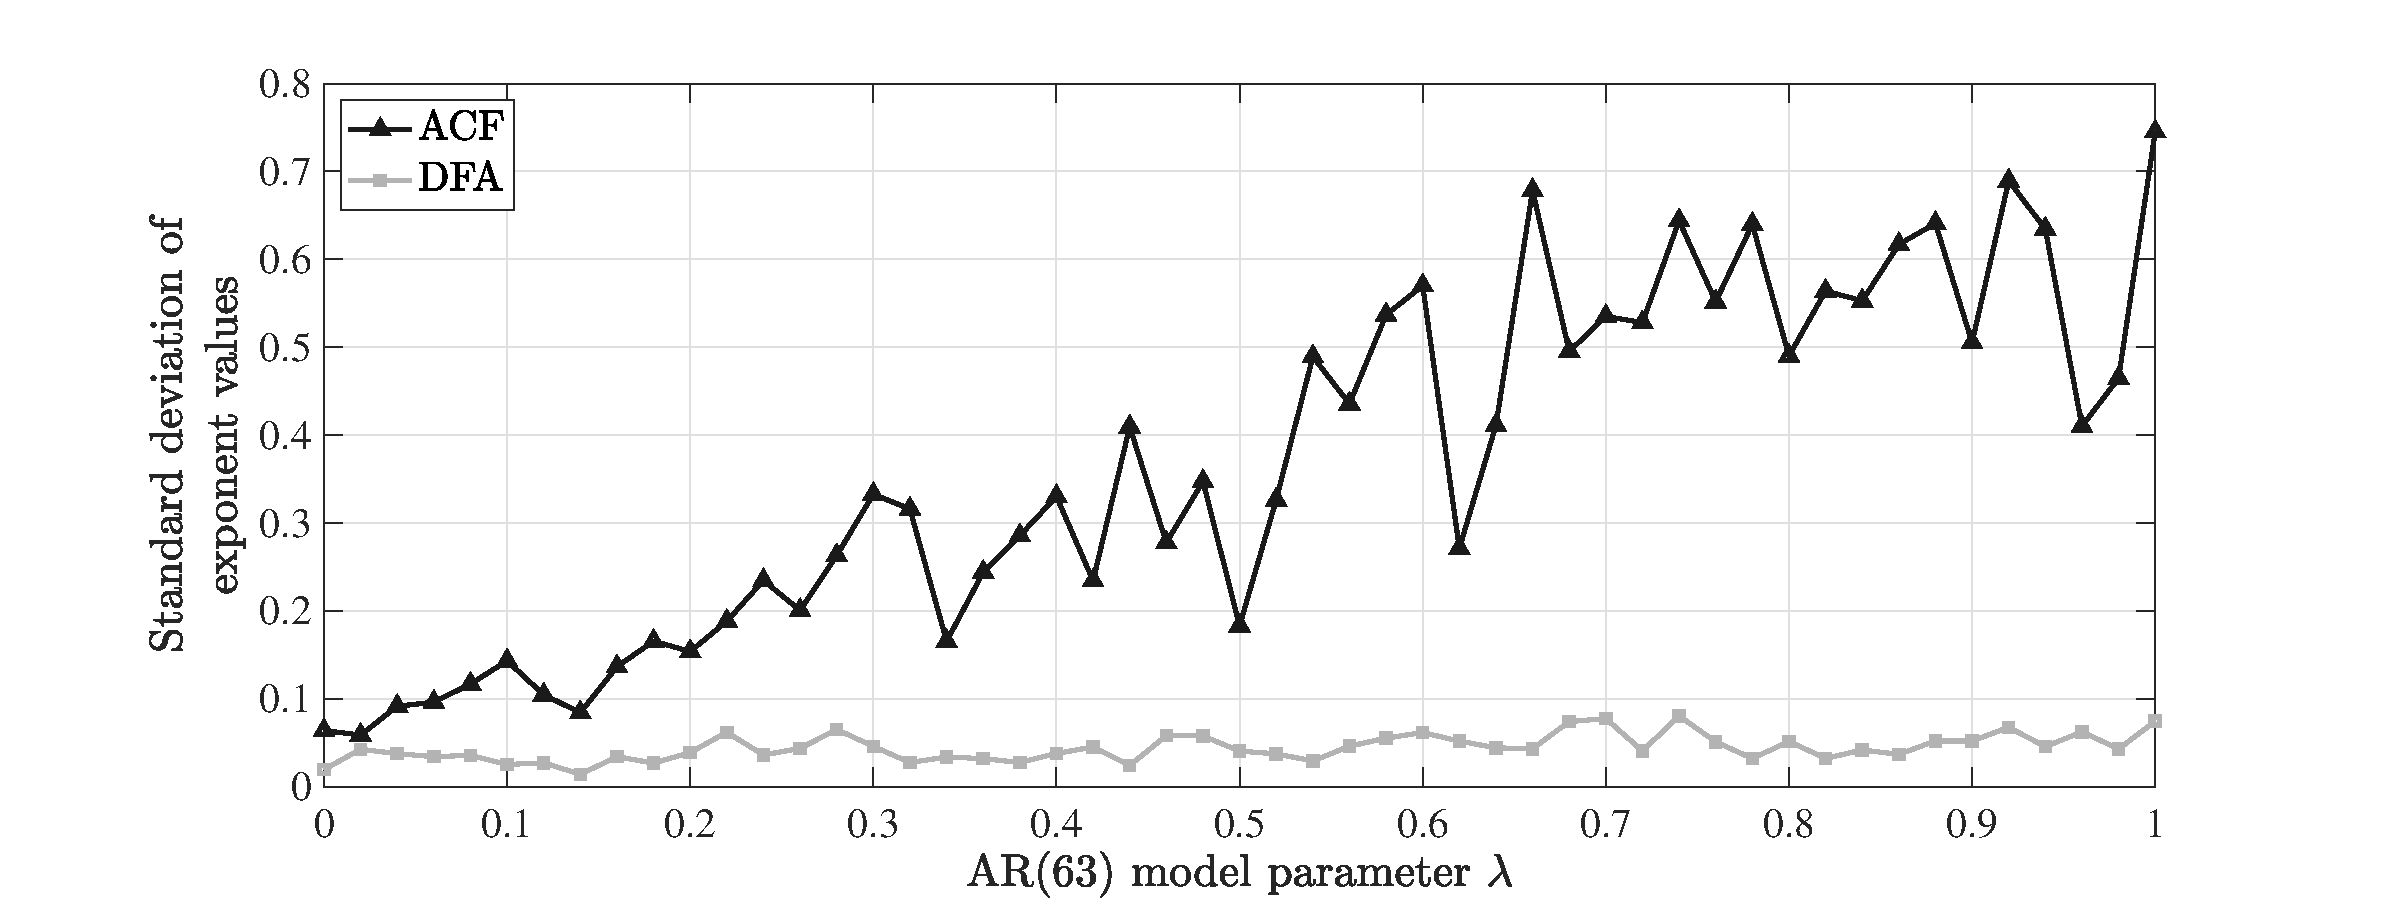
\includegraphics[width = 0.9\textwidth]{f4_ACF_DFA_reliability_v2}
	\caption{Standard deviation of the ACF and DFA scaling exponents over 50 noise series of length 1000, for each noise correlation parameter $\lambda = 0, 0.02, 0.04, ..., 1$. The mean values of the exponents range between 0 and 1.2 (ACF), and between 0.5 and 1 (for DFA).}
	\label{fig:1D:ACFDFAreliability}
\end{figure}
 

\subsubsection{The relationship between $\gamma$ and the lag-1 autocorrelation}

We also investigate the relationship between the ACF scaling exponent and the simple lag-1 autocorrelation function (ACF1). While the ACF exponent is unreliable and the superior DFA exponent has been introduced specifically as a more reliable measure \citep{kantelhardt2001}, the ACF1 has been widely used in tipping-point research \citep{held2004,dakos2008} and is much less computationally expensive than the calculation of the scaling exponents detailed in this chapter. 

Figure \ref{fig:1D:ACFrelationships} shows the ACF scaling exponent and the ACF1 calculated for 200 short-range correlated noise series (panel {\bf a}), and 200 long-range correlated noise series (panel {\bf b}), with varying correlation parameters. The short-range correlated noise is produced using an AR(1) model (equation \ref{eqn:1D:AR1_model}) and the long-range correlated noise is produced using the AR(63) model \citep{kasdin1995}.

We note that the lag-1 ACF is an estimator of the AR(1) model parameter $\lambda$ and we would expect the two values to be approximately equal, which is evident in figure \ref{fig:1D:ACFrelationships} panel {\bf a}. The ACF scaling exponent, however, does not respond to any increase in the parameter below the value of $\lambda= 0.7$, although it does increase with increasing $\lambda$ for larger values when the noise can be said to be "red". For low values of $\lambda$ the autocorrelation functions with lag $\geq2$ are approximately zero and so the ACF decays exponentially after lag-1 making it essentially useless. The behaviour is similar in the DFA and PS exponents, we now note the cluster of points in figure \ref{fig:1D:ExponentRelationships} panel {\bf b} for low exponent values, because a measure of scaling is not suitable for this particular short-range correlation. We note also that the ACF exponent displays large variability for $\lambda>0.7$, as already noted for long-range correlated noise (see figure \ref{fig:1D:3exponents_rednoise}). 

In figure \ref{fig:1D:ACFrelationships} panel {\bf b} we see that the lag-1 ACF increases linearly with the AR(63) model parameter $\lambda$ until $\lambda=1$ (red noise) after which it tends to its maximum value 1. The ACF scaling exponent also increases, apparently linearly, with $\lambda$, until $\lambda\approx0.7$ after which it decreases to zero. In the case of the AR(1) model with $\lambda<0.7$ the ACF exponent is zero because the ACF for all lags in the range $[10, 100]$ is zero and so the linear fit to the points in this range has a slope of zero. In contrast, the AR(63) model with $\lambda=2$ also has an ACF exponent close to zero but because the ACF for all lags in the range $[10, 100]$ is close to 1. Over 1000 noise series were produced using the same AR(63) model, with $\lambda=2$, in order to evidence the phenomenon. The lag-10 ACF had a mean value of 0.98 and the lag-100 ACF had a mean value of 0.83. 


\begin{figure}
	\centering
	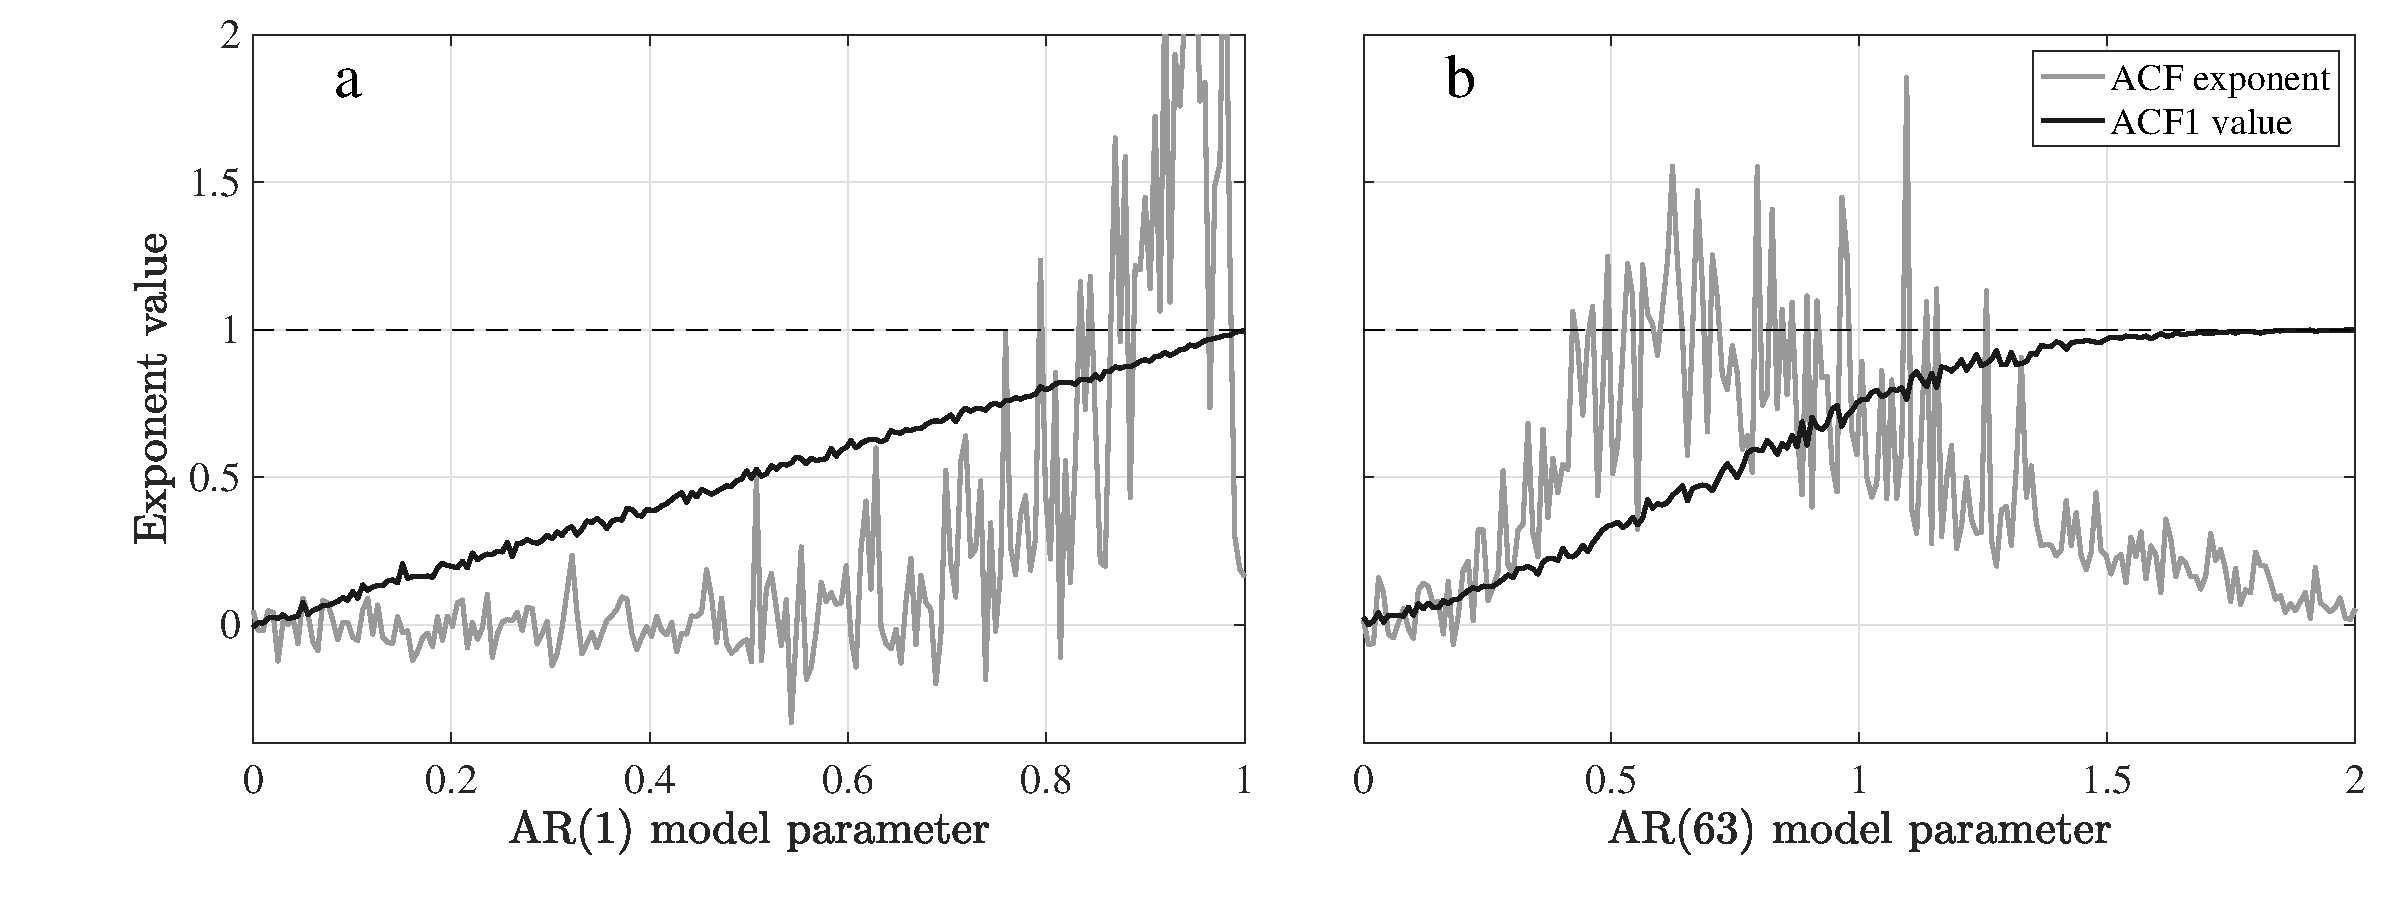
\includegraphics[width=0.9\textwidth]{f5_ACFRelationships_v2}
	\caption{ACF scaling exponent and the simple lag-1 ACF for 200 short-range correlated noise series (panel {\bf a}), and 200 long-range correlated noise series (panel {\bf b}), with varying correlation parameters.}
	\label{fig:1D:ACFrelationships}
\end{figure}






\section{Use of scaling exponents for Early Warning Signals}
%\section{Use of scaling exponents as Early Warning Signals: the ACF1, DFA and PS indicators}
\label{sec:1D:Exponents_as_EWS}


\subsection{Critical slowing down as an AR(1) process}
\label{subsec:1D:Exponents_as_EWS:CriticalSD}

The phenomenon of \emph{critical slowing down} is observed in a broad range of dynamical systems exhibiting tipping behaviour \citep{scheffer2001,lenton2008,scheffer2009,scheffer2009critical,lenton2012}. The `slowing down' to which the phrase refers is the longer and longer times taken by the system to return to the equilibrium state, given a random perturbation, in the time preceding a tipping point. At some \emph{critical} point, that is, the tipping point, the return time becomes effectively infinite\footnote{Of course, a separate tipping event may occur at which time the system returns to that original stable state.} as the system leaves that equilibrium state forever. 

The use of the autocorrelation scaling exponent as an EWS is justified by modelling a dynamical system using a one-dimensional autoregressive system:
	\begin{equation}
	\label{eqn:1D:AR1_decay_model}
		z_{n+1} = e^{-\kappa\Delta t}z_{n} + \sigma\eta_n\,,
	\end{equation}
\citep{held2004, scheffer2009} where $\sigma$ is a constant and $\eta_n$ is a white noise term. The model considers the equilibrium state $z_n=0$ as the critical mode of a system undergoing a bifurcation. The system returns to equilibrium exponentially with rate $\kappa$, the decay rate. During a bifurcation a system will undergo critical slowing down, that is, a decreasing rate $\kappa$. The autocorrelation coefficient $\alpha \equiv e^{-\kappa\Delta t}$ increases to $1$ as $\kappa$ decreases to zero. The autoregressive model parameter $\exp(-\kappa\Delta t)$, and thus the simple lag-1 autocorrelation function (ACF1), will clearly also increase as $\kappa$ decreases. The ACF1 is therefore also a possible EWS indicator and is widely used \citep{held2004,lenton2012}. As noted by \citet{scheffer2009}, it is often the case that as the autocorrelation increases so does the variance, this is true of the AR(1) process described by equation \ref{eqn:1D:AR1_decay_model} where the expectation is zero and the variance is given by
	\begin{equation}
		\text{Var}(z_n) = \frac{\sigma^2}{1-\alpha^2}\,,
	\end{equation} 
where $\alpha=\exp(-\kappa\Delta t)$ is the autocorrelation coefficient. Thus detecting an increase in variance will provide an additional EWS.

As an example of critical slowing down, we consider the bifurcating dynamical system given by the differential equation 
	\begin{equation}
		\frac{dz}{dt} = -\frac{\partial}{\partial z}U\,,
	\label{eqn:1D:ExamplePitchforkEquation}
	\end{equation}
where $U$ is the generalised potential function given by $U = z^4 + \mu z^2$, where $\mu$ is a parameter which may vary with time. If $\mu$ is positive and decreases with time, the system is an example of a pitchfork bifurcation with a decaying stable mode at $z=0$. For $\mu<0$ this mode becomes unstable and two stable modes are created at $z=\pm\sqrt{-\mu/2}$. The shape of the generalised potential function $U$ is illustrated in figure \ref{fig:intro:ChangingPotential}. Differentiating $U$, we rewrite equation \ref{eqn:1D:ExamplePitchforkEquation} as
	\begin{equation}
		\frac{dz}{dt} = -4z^3-2\mu z = f(z)\,.
	\label{eqn:1D:SimpleExamplePitchforkEquation}
	\end{equation}
We now consider the $\mu>0$ system with a small perturbation from the stable mode, that is, $z=\varepsilon$. Linearising  equation \ref{eqn:1D:SimpleExamplePitchforkEquation} using the first-order Taylor expansion around the stable mode $z=0$ gives
	\begin{equation}
		\left.\frac{dz}{dt}\right|_\varepsilon = f(\varepsilon) \approx -2\mu\varepsilon\,.
	\label{eqn:1D:TaylorExp}
	\end{equation}
So, for $\mu>0$, the system goes exponentially to zero. When $\mu=0$ the recovery rate $\m2\mu$ is zero and so the system will not recover from the small perturbation $\varepsilon$. When $\mu<0$ the mode $z=0$, as noted, is unstable and system will go exponentially away from zero. If it is assumed that a dynamical system possesses a critical mode, that is, a mode that is decaying as a result of a bifurcation, then the recovery rate of this mode will go to zero as the system takes longer (eventually infinite time, after the bifurcation) to return to the stable state after a perturbation. The tendency of the system in one direction can be measured by an increase in the lag-1 autocorrelation function (ACF1), thus this is a reasonable indicator of the decreasing decay rate. 

The hypothesis is that this critical slowing down will be seen in a wide variety of dynamical systems approaching a bifurcation. \citet{van2007} test this hypothesis with a number of ecological models and find that the intensity of the critical slowing down effect is linearly, or almost linearly, related to the distance from the tipping point in all cases.



\citet{held2004} use a rise in ACF1 as an indicator of a bifurcation in a model of North Atlantic thermohaline circulation. The measured variables are presumed to represent a dynamical system undergoing a bifurcation and therefore possessing a critical mode. In order to determine the point at which the ACF1 value rises, a method is used labelled "degenerate fingerprinting" by \citet{held2004}. The ACF1 of the data, in this case the Atlantic overturning flux, is calculated in sequential, overlapping windows so that the ACF1 value can be tracked over time. If the value is expected to rise, or begin to rise, before the tipping point, the increase in the ACF1 is an early warning signal of the tipping. 


\subsection{Early warning indicators}
\label{subsec:1D:Exponents_as_EWS:indicators}

\subsubsection{Lag-1 autocorrelation as an indicator}
{\Red
By measuring the lag-1 ACF of a time series in a sliding fixed-length time window, the value of this statistic becomes a function of time and the increase or decrease in the value over time may act as an \emph{indicator} of a tipping point. We refer to this time-dependent lag-1 ACF as the \emph{ACF1 indicator}, giving us the following definition:
}
\begin{definition} [The ACF1 indicator]
	\label{def:1D:indicator:ACF1}
	For time series data 
	\begin{equation}
		[x_t] = x_1, x_2, x_3, ..., x_N
	\end{equation}
	we create a new indicator series $[Y_t]$:
	\begin{equation}
	\label{eqn:1D:ACFfingerprinting}
		Y_t = \text{ACF}_1([x_{t-w+1},...,x_t]) ~~\text{for}~~t\geq w,
	\end{equation}
	where $w$ is the window size, typically $\leq 10\%$ of the time series length $N$. The first $w-1$ values of $[Y_t]$ are omitted. 
\end{definition}
{\Red The resulting \emph{signal}, that is, the time series of the $Y_t$ plotted over time, we refer to as an \emph{Early Warning Signal}. This method is used throughout this study and, particularly when observed physical data is used in chapter \ref{chap:cyclones}, careful attention is paid to the choice of the window size $w$. }

\subsubsection{The DFA indicator}

\citet{livina2007} modify the ACF1 indicator so that the DFA exponent is calculated instead of the lag-1 autocorrelation function in each window of data:
\begin{definition} [The DFA indicator]
	\label{def:1D:indicator:DFA}
	For time series data $[x_t] = x_1, ..., x_N$ we calculate the DFA scaling exponent $\alpha$ (see definition~\ref{def:1D:DFAexponent}) for consecutive overlapping windows $[x_{t-w+1},...,x_t]$ where $w$ is the `window size' to be determined (typically $\leq 10\%$ of the time series length $N$. We then have a sequence of values of $\alpha$:
	\begin{equation}
	\label{eqn:1D:DFAfingerprinting}
		\alpha_t = \text{DFA}([x_{t-w+1},...,x_t]) ~~\text{for}~~t\geq w\,.
	\end{equation}
	The function $\text{DFA}(\cdot)$ denotes the calculation of the order DFA exponent $\alpha$ for the truncated length-$w$ time series. The DFA indicator A(t) is this series of scaling exponent values expressed as a function of time:
	\begin{equation}
		A(t) = \alpha_t\,.
	\end{equation}
	In numerical implementations we set $A(t)=0$ for $t<w$.
\end{definition}
In this study, we consistently use the order-2 DFA exponent, but the indicator may also be used with higher orders. \citet{livina2007} test the DFA indicator method on data from a model of Atlantic overturning circulation \citep{edwards2005} and also Greenland paleotemperature records \citep{alley2000}. The DFA indicator is also compared to the ACF1 indicator \citep{lenton2012} where it is concluded that both methods offer their own pros and cons. In particular, computing the DFA exponent for every window of data is computationally expensive. 

\subsubsection{The PS exponent as an early warning indicator}
The possibility of such modification of the fingerprinting method allows us to instead use the power spectrum (PS) scaling exponent, which is obtained from the periodogram as in section \ref{subsec:1D:scaling_exponents:PS}, \citep{prettyman2018}. \citet{kleinen2003} notes already that spectral properties of the time series may also be used as tipping point indicators, in particular when the tipping point is associated with a change in the structure of the noise or a stationary system becoming non-stationary. A shift from a dominance of short-scale memory to long-scale memory, seen in the measurement of the PS scaling exponent, will be associated with a rise in autocorrelation. In this respect, therefore, the PS exponent and the ACF are related, further justifying the use of the PS exponent as an EWS. There also exists a relationship between the PS exponent and the DFA exponent \citep{heneghan2000, kantelhardt2001} as explained in section \ref{sec:1D:relationships}. We note that although \citet{heneghan2000} advises that there is no difference between the DFA and PS exponents, and that therefore it is not necessary to use both, this applies only for long-range correlated data. The relationship is investigated in section \ref{sec:1D:relationships}: while figure \ref{fig:1D:ExponentRelationships}b shows the linear relationship proposed by \citet{kantelhardt2001}, figure \ref{fig:1D:ExponentRelationships}a shows a non-linear relationship in the experiment where short-range correlated noise is used. We thus see that the relationship between the two exponents may vary depending on the nature of the data. In a system where the correlation in the time series changes over time, and trends or feedbacks affect the dynamical system, there may not exist an analytic relationship between the DFA and PS exponents and the use of one may therefore reveal information that the use of the other cannot. 

We therefore propose the use of the power spectrum indicator, alongside the DFA and ACF1 indicators. The PS exponent is estimated by calculating the negative slope of the periodogram, produced using a fast Fourier transform, in the frequency range $[10^{\m1}, 10^{\m2}]$. This is done for in a sliding window according to the fingerprinting method \citep{held2004,livina2007}. 

\begin{definition} [The PS indicator]
	\label{def:1D:indicator:PS}
	For time series data $[x_t] = x_1, ..., x_N$ we calculate the PS exponent $\beta$ (See definition \ref{def:1D:PSexponent}) for consecutive overlapping windows $[x_{t-w+1},...,x_t]$, where $w$ is the window size to be determined. We then have a sequence of $\beta$ values
	\begin{equation}
	\label{eqn:1D:PSindicator:exponent_beta}
		\beta_t = \text{PS}([x_{t-w+1},...,x_t]) ~~\text{for}~~t\geq w\,.
	\end{equation}
	The function $\text{PS}(\cdot)$ denotes, in this instance, the calculation of the power spectrum scaling exponent $\beta$ as the negative slope of the periodogram which approximates the power spectrum $S_x(f)$. The PS indicator $B(t)$ is this exponent expressed as a function of time, that is,
	\begin{equation}
		\label{eqn:1D:PSfingerprinting}
		B(t) = \beta_t\,.
	\end{equation}
	In numerical implementations we set $B(t)=0$ for $t<w$.
\end{definition}

{\Red{
		
If we consider the AR(1) model, which is used as the prototypical example of the critical slowing down phenomenon as in equation~\ref{eqn:1D:AR1_decay_model} (see section~\ref{subsec:1D:Exponents_as_EWS:CriticalSD} and \cite{scheffer2009}), we can reason that the PS exponent may provide an EWS. In that case, the critical slowing down in a system is modelled by the AR(1) process
	\begin{equation}
	\label{eqn:1D:PSindicator:AR1model}
		z_{n+1} = \mu z_{n} + \sigma\eta_n\,,
	\end{equation}
where $\eta_n$ is a white noise term and where the parameter $\mu=e^{-\kappa\Delta t}$ is determined by the \emph{decay rate} $\kappa$ which decreases to zero as the tipping point approaches, modelling the increasing time taken for a system to return to equilibrium after a small perturbation. For the PS indicator $B(t)$ to provide an EWS, we require that the value of $\beta$ changes as $\mu$ increases, that is, as the tipping point approaches. The value of $\beta$ can be obtained analytically from the power spectrum of the AR(1) process, which is given by
	\begin{equation}
	\label{eqn:1D:PSindicator:AR1powerspectrum}
		\begin{split}
		S_x(f) &= \frac{\sigma^2}{\left|1-\mu e^{\m2\pi i f}\right|^2}\\
		&= \frac{\sigma^2}{1+ \mu^2 - 2\mu\cos(2\pi f)}\,,
		\end{split}
	\end{equation}
\citep{vonstorch}. The power spectrum scaling exponent $\beta$ is then given by the negative gradient of $S_x(f)$ on a logarithmic scale, or the logarithm of $S_x(f)$ differentiated with respect to $\log f$, which gives, 
	\begin{equation}
		\beta_f = -\frac{d}{d(\log f)}\log\left[S_x(f)\right]\,.
	\end{equation}
We note that here $\beta$ depends on the frequency $f$ since the AR(1) power spectrum does not exhibit true power-law scaling; cases such as this are considered more thoroughly in section~\ref{subsec:1D:Exponents_as_EWS:nopowerlawsacaling}. In numerical calculations of the PS indicator series, the linear fit to the periodogram is taken over the interval $10^{\m2}\leq f \leq 10^{\m1}$ (see definition~\ref{def:1D:PSexponent}), the reasons for this choice of the frequency range are discussed in section~\ref{subsec:1D:Exponents_as_EWS:determining_frequency_range} and are based on taking the AR(1) process as the model of critical slowing down. 

In order to obtain a single value for $\beta$ we integrate equation~\ref{eqn:1D:PSindicator:AR1powerspectrum} over the entire range $10^{\m2}\leq f \leq 10^{\m1}$, or $\m2\leq \log f \leq\m1$, 
	\begin{equation}
	\begin{split}
		\beta &= \int_{\m2}^{\m1}-\frac{d\log\left[S_x(f)\right]}{d(\log f)}d(\log f)\\
		&= \left. \m\log\left[S_x(f)\right] \right|_{\log f = \m2}^{\m1}\\
		&= \left. \m\log\left[  \frac{\sigma^2}{1+\mu^2-2\mu \cos(2\pi f)}  \right] \right|_{\log f = \m2}^{\m1}\,,
	\end{split}
	\end{equation}
which gives 
	\begin{equation}
	\label{eqn:1D:PSindicator:PSofAR1}
		\beta = \log\left[  \frac{1+\mu^2-2\mu \cos(0.2\pi)}{1+\mu^2-2\mu \cos(0.02\pi)}  \right] \,.
	\end{equation}
This value of the PS exponent $\beta$, using this equation, is plotted in figure~\ref{fig:1D:PSofAR1}a for values of $\mu$ between $0$ and $1$. We note that $\beta$ increases from $0$ to $2$ as $\mu$ increases, that is, as the modelled critical slowing down becomes more pronounced. We therefore expect that the PS indicator $B(t)$, which tracks the value $\beta$ as a function of time, will provide an early warning signal of tipping points for which the critical slowing down phenomenon occurs, and we can expect that the PS exponent value will be $\approx 2$ when the decay rate $\kappa$ has decreased to zero ($\mu=1$ in equation~\ref{eqn:1D:PSindicator:AR1model}). In order to test the proposed relationship between the PS exponent $\beta$ and the AR(1) model parameter $\mu$, as shown in equation~\ref{eqn:1D:PSindicator:PSofAR1}, the results of an experiment are presented in figure~\ref{fig:1D:PSofAR1}b: $200$ AR(1) processes are modelled as time series of length $10^5$, each with parameter $\mu$ between $0$ and $1$. For each of the $200$ time series $X$ the PS exponent is estimated numerically in the frequency range $\m2\leq\log f\leq\m1$ and the lag-1 ACF is also calculated, the numerically-obtained PS exponent $\text{PS}(X)$ is plotted against the lag-1 autocorrelation $\text{ACF1}(X)$ in figure~\ref{fig:1D:PSofAR1}b. We note that the relationship found analytically in equation~\ref{eqn:1D:PSindicator:PSofAR1} (plotted in figure~\ref{fig:1D:PSofAR1}a) is verified by the numerical results, thus verifying the numerical method of obtaining the PS exponent (see definition~\ref{def:1D:PSexponent}).

Given a time series obtained from an AR(1) process with parameter $\mu$, that is,
\begin{equation}
	z_{n+1} = \mu z_n + \eta_n,
\end{equation}
with $\eta_n$ independent Gaussian white noise terms, we can reconstruct the value $\mu$ from the time series only by calculating the PS exponent $\beta$ in the frequency range $\m2\leq\log f\leq\m1$. We simply solve equation~\ref{eqn:1D:PSindicator:PSofAR1} for $\mu$ to obtain
\begin{equation}
	\label{eqn:1D:PSindicator:reconstruct_mu}
	\mu\approx b-\sqrt{b^2-1}~~~\text{where}~~~ b = \frac{\cos(0.2\pi)-10^\beta \cos(0.02\pi)}{1-10^\beta}.
\end{equation}
This result may appear counter-intuitive given that the power spectrum of the AR(1) process does not actually exhibit power-law scaling, but we see clearly in figure~\ref{fig:1D:PSofAR1} that the values obtained using this equation correlate with the lag-1 autocorrelation. This relationship, and the relevance of the PS indicator in systems where the power spectrum does not have power-law scaling, are investigated further in sections~\ref{subsec:1D:Exponents_as_EWS:nopowerlawsacaling} and~\ref{subsec:1D:Exponents_as_EWS:determining_frequency_range}.
}}

\begin{figure}
	% plotted using the Matlab script 'PSofAR1.m'
	\centering
	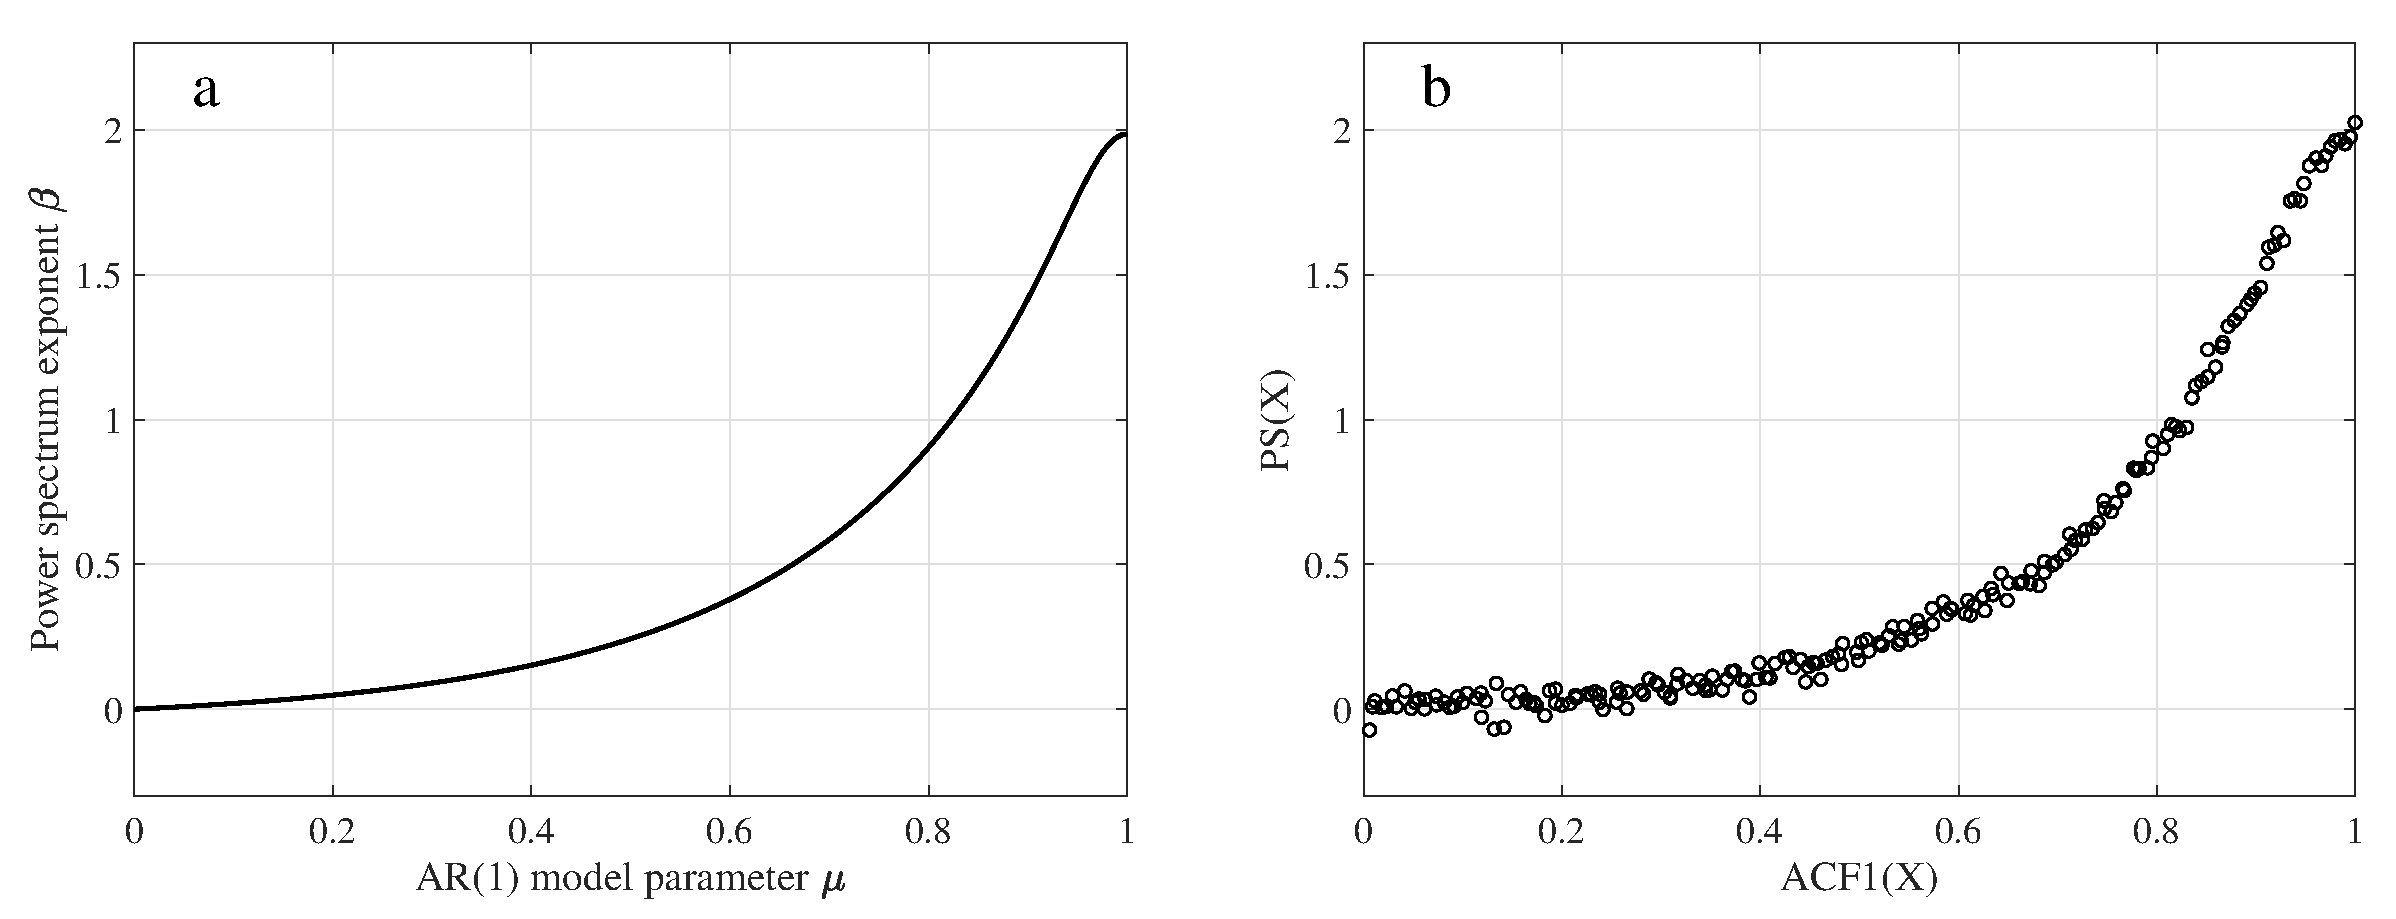
\includegraphics[width=0.9\linewidth]{PSofAR1}
	\caption{\label{fig:1D:PSofAR1}
		{\Red Panel {\bf a}: The relationship between the PS scaling exponent $\beta$ and the parameter $\mu$ of the AR(1) process is plotted for $0\leq\mu\leq 1$ (see equation~\ref{eqn:1D:PSindicator:PSofAR1}). Panel {\bf b}: The PS exponent and lag-1 autocorrelation is calculated for $200$ AR(1) time series $X$ of length $10^5$ and the results plotted against each other. The relationship between these numerically-obtained values confirms the derivation of equation~\ref{eqn:1D:PSindicator:PSofAR1} and the accuracy of the numerical methods.}
	}
\end{figure}

\subsubsection{The ACF scaling exponent as an early warning indicator}

{\Red{

As we have defined the DFA indicator $A(t)$ based on the DFA scaling exponent $\alpha$, and the PS indicator $B(t)$ based on the PS scaling exponent $\beta$, we have neglected the ACF scaling exponent $\gamma$ (see definition~\ref{def:1D:ACFexponent}), from which we might define the ACF scaling indicator $\Gamma(t)$ in much the same way. However, this is not often used as an early warning indicator in the literature and the DFA scaling exponent has been developed as a superior alternative to the ACF scaling exponent \citep{kantelhardt2001}: this has since been used successfully as an early warning indicator \citep{livina2007}. When testing the effectiveness of the novel PS indicator we therefore use the DFA indicator as a benchmark.

Another useful benchmark test for a novel indicator is whether it is effective in detecting a change in the model parameter of the AR(1) process, since this is used as a model of critical slowing down (see section~\ref{subsec:1D:Exponents_as_EWS:CriticalSD}). In figure~\ref{fig:1D:ACFrelationships} we have already demonstrated the superior performance of the simple lag-1 autocorrelation over the ACF scaling exponent, and the ACF1 indicator is used throughout this thesis for comparison with the PS indicator. For these reasons, we do not use what we might call the `ACF scaling indicator' but look to the ACF1 indicator and the DFA indicator instead.

}}

\subsection{Early warning indicators in the absence of power-law scaling}
\label{subsec:1D:Exponents_as_EWS:nopowerlawsacaling}

{\Red{
The definitions of all scaling exponents, and thus early warning indicators, assume the existence of power-law scaling. For example, in the case of the PS exponent we assume the power spectrum $S(f)$, which is approximated by the periodogram, is of the form $S(f)\sim f^{-\beta}$ for some exponent $\beta$, and it is this value that we seek to measure. However, it is unlikely that we will find true power-law scaling like this in dynamical systems or data from real-life processes unless we are dealing with pure white noise or a pure random walk. Indeed we note that the common stochastic model, the AR(1) process, with which we model critical slowing down \citep{scheffer2009critical}, does not even have true power-law scaling in the power spectrum. 

In this section we show that it is still a valuable exercise to measure the PS exponent in cases in which there is no true power-law scaling. In particular, we focus on cases for which there is \emph{crossover} in the power spectrum, that is, when the power spectrum follows one power-law scaling relationship at low frequencies and another at higher frequencies, with a crossover at some midpoint. In the following  section~\ref{subsec:1D:Exponents_as_EWS:determining_frequency_range} we concentrate specifically on the AR(1) model which is of importance to tipping point research, and which also contains a power spectrum crossover.
}}

\subsubsection{Power spectra containing crossovers}
{\Red{
To create a time series with a clear crossover in the power spectrum we take the sum of a Gaussian white noise series $\eta_t$ and red noise (random walk) series $W_t$ defined by the relation $W_t = W_{t-1} + \zeta_t$, where $\zeta_t$ are a Gaussian white noise series independent of $\eta_t$. Thus the terms of the series are given by
	\begin{equation}
	\label{eqn:1D:crossoverfunction}
		z(t) = \left(\sum_{\tau=0}^t \zeta_\tau\right) + \mu\eta_t\,,
	\end{equation}
where $\mu$ is a parameter modifying the variance of the white noise terms $\eta_t$. Due to the linearity of the Fourier transform we are able to calculate the power spectrum $S_z(f)$ of this series given that we know already
	\begin{equation}
	\label{eqn:1D:powerspectrum_white}
		S_{\mu\eta}(f) = \left| \mu\hat{\eta}(f) \right|^2 = \mu^2
	\end{equation}
since $\hat{\eta}(f)=1$, and
	\begin{equation}
	\label{eqn:1D:powerspectrum_red}
		S_{W}(f) = \left| \hat{W}(f) \right|^2 = \left|\frac{1}{2\pi f}\right|^2 = \frac{1}{4\pi^2}f^{\m2}.
	\end{equation}
Combining the two series we have
	\begin{equation}
	\begin{split}
		S_z(f) &= \left| \hat{z}(f) \right|^2\\
		&= \left| \hat{W}(f) + \mu\hat{\eta}(f) \right|^2\\
		&= \left| \frac{1}{2\pi f} + \mu\right|^2\\
		\label{eqn:1D:powerspectrum_cross}
		&= \frac{1}{4\pi^2}f^{\m2} + \frac{\mu}{2\pi}f^{\m1} + \mu^2\,.
	\end{split}
	\end{equation}
}}

\begin{figure}
	\centering
	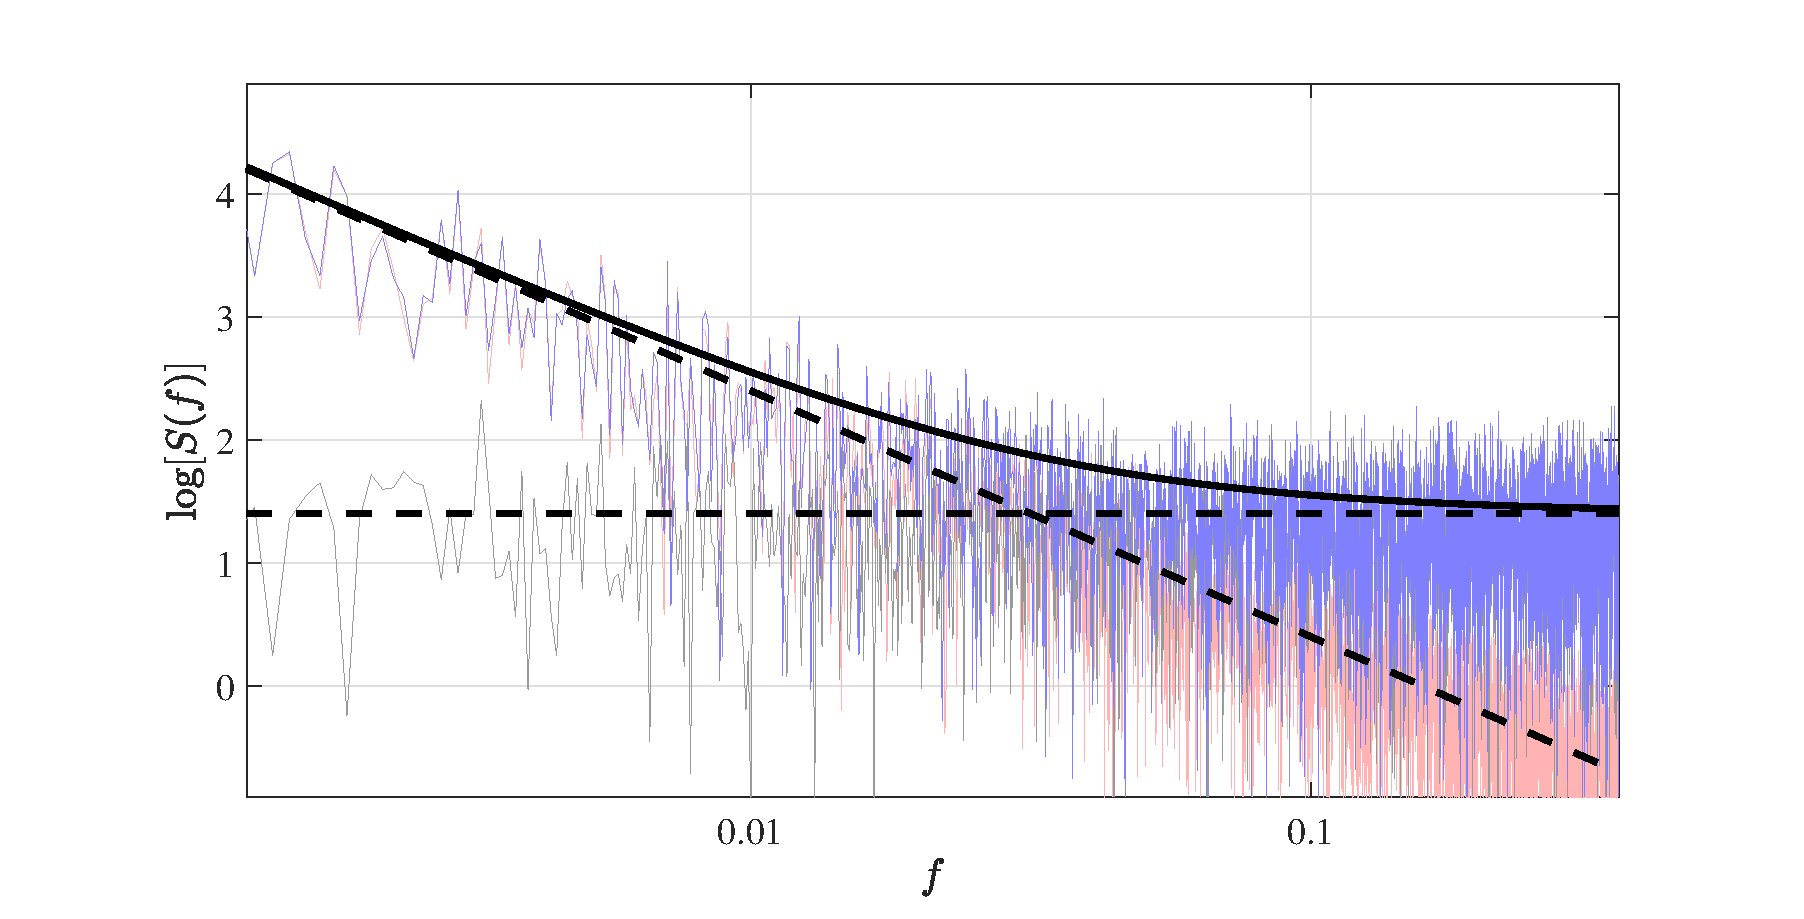
\includegraphics[width=\linewidth]{crossover1}
	\caption{\label{fig:1D:crossover1}
		{\Red Scaling crossover in the power spectrum of the sum of red and white noise series. Showing the power spectrum of the series $z(t)$ (solid black line, see equation~\ref{eqn:1D:crossoverfunction}) imposed over the periodogram (blue). Also showing the power spectrum of white and red noise (dashed black lines) and their periodograms (grey and red respectively). The crossover occurs at $f=10^{-3/2}$ (see equation~\ref{eqn:1D:crossoverfrequency}).}
	}
\end{figure}

{\Red{
In figure~\ref{fig:1D:crossover1} the power spectra of white noise $\mu\eta_t$ and red noise $W_t$, given by equations~\ref{eqn:1D:powerspectrum_white} and~\ref{eqn:1D:powerspectrum_red} respectively, are shown (dashed lines) imposed over the periodograms of computed instances of these series (shown in grey and red respectively). In this case the value 
	\begin{equation}
		\mu = \frac{10^{3/2}}{2\pi}
	\end{equation}
has been chosen so that the intersection of the two curves, given by equations~\ref{eqn:1D:powerspectrum_white} and~\ref{eqn:1D:powerspectrum_red} is given by 
	\begin{align}
	\label{eqn:1D:crossoverfrequency}
		\begin{split}
		\frac{1}{4\pi^2}f^{\m2} &= \mu^2,\\
		\frac{1}{2\pi}f^{\m1} &= \mu,\\
		\frac{1}{2\pi}f^{\m1} &= \frac{10^{3/2}}{2\pi},\\
		f &= 10^{\m3/2}\,,
		\end{split}
	\end{align}
which is the midpoint of the values $f=0.01$ and $f=0.1$ on the logarithmic scale. In figure~\ref{fig:1D:crossover1} we also see the power spectrum of the function $z(t)$, given by equation~\ref{eqn:1D:powerspectrum_cross} (solid line), and the periodogram of an instance of the time series (shown in blue). This time series is simply the sum of the white noise and red noise series. We note that the periodogram of $z$ entirely overlaps the periodogram of the red noise series $W$ for small values of $f$, and overlaps the periodogram of the white noise series $\eta$ for large values of $f$. 
}}

\subsubsection{Applying the PS indicator}
	\begin{figure}
		\centering
		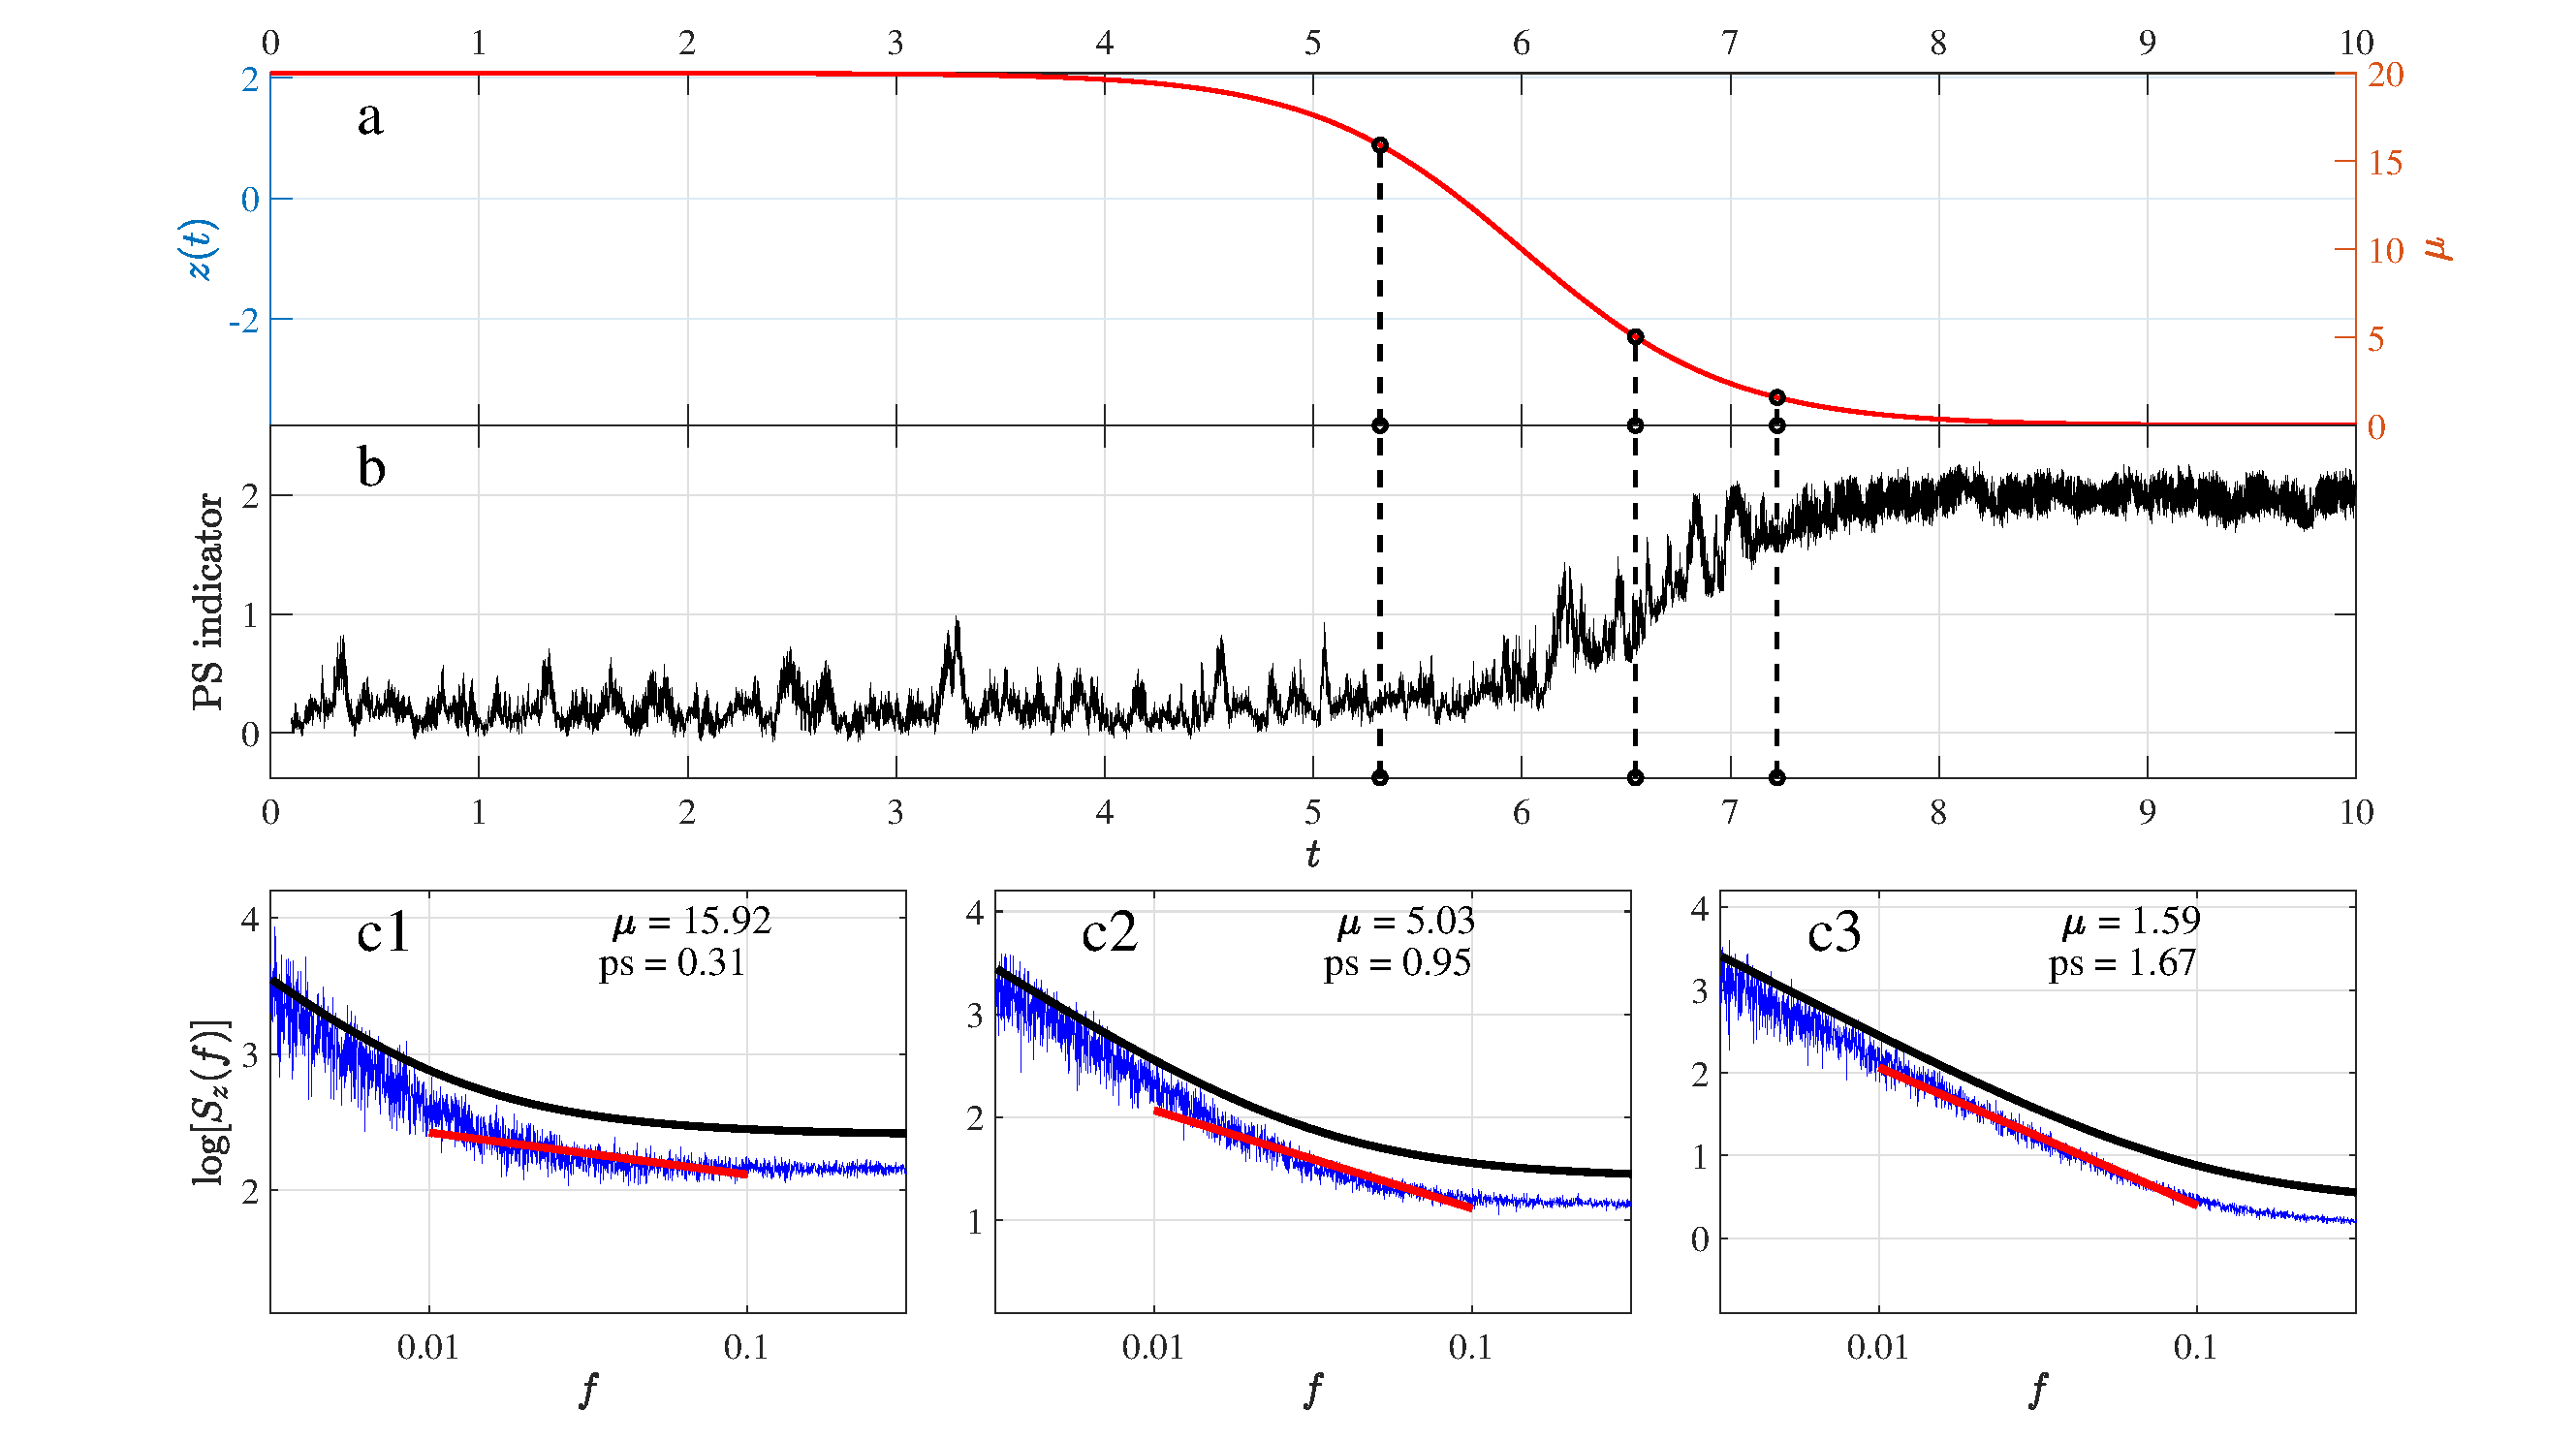
\includegraphics[width=\linewidth]{crossover2_decrease}
		\caption{\label{fig:1D:crossover2}
			{\Red Power spectrum indicator of the sum of white noise and red noise series with decreasing white noise component. Panel {\bf a}: The time series $z(t)$ (blue, left $y$-axis) and the standard deviation $\mu$ of the white noise component (red, right $y$-axis). The dashed black lines show times at which the crossover point is at the lower end, the centre, and the upper end of the frequency range in which the PS indicator is measured. Panel {\bf b}: The PS indicator in a sliding window $1\%$ of the length of the time series. Panels {\bf c}: Depictions of the periodograms of $z(t)$ when the crossover point is at the lower end, the centre, and the upped end of the measured frequency range (panels c1, c2, c3 respectively). The power spectrum (black) and the linear fit to the periodogram (red) and also shown.}
		}
	\end{figure}
{\Red{
The power spectrum of $z(t)$, given by equation~\ref{eqn:1D:powerspectrum_cross}, does not exhibit simple power-law scaling, since there is no value $\xi$ for which 
	\begin{equation}
		S_z(cf) = c^\xi S_z(f)\,,
	\end{equation}
and so the power spectrum is not simply a straight line in the log-log plot (figure~\ref{fig:1D:crossover1}). However, this does not mean that there is no value in applying the Power Spectrum indicator, which simply fits a straight line to the periodogram to obtain a single value $\xi$. When applying the PS indicator to dynamical systems with tipping behaviour it is not the exact value of the indicator that is of interest but the change in the value over time as the indicator is applied in a sliding window on the time series. In particular we are concerned with the detection of critical slowing down in the time before a tipping point is reached which is characterised by an increase in the autocorrelation scaling exponent, or a ``reddening'' of the power spectrum as the return time around a stable state increases. 

In figure~\ref{fig:1D:crossover2}a we have plotted the series $z(t)$ given by equation~\ref{eqn:1D:crossoverfunction}, the sum of a red noise and a white noise series with scaling crossover (blue line, left $y$-axis). In this case the value of the parameter $\mu$ changes with time and is described by the function
	\begin{equation}
		\mu(t) = 10-10\tanh(t-6),
	\end{equation}
so that $\mu\rightarrow20$ as $t\rightarrow-\infty$ and $\mu\rightarrow0$ as $t\rightarrow\infty$. This function is plotted alongside the time series in figure~\ref{fig:1D:crossover2}a (red line, right $y$-axis). We note that the value of $f$ at which the crossover occurs in the power spectrum is given by 
	\begin{equation}
		f_\text{c} = \frac{1}{2\pi\mu},
	\end{equation}
(see equation~\ref{eqn:1D:crossoverfrequency}) and therefore varies with the value of $\mu$. For this experiment, when applying the PS indicator, we have chosen to estimate the slope of the periodogram in the frequency range $10^{\m2}\leq f \leq 10^{\m1}$. For large values of $\mu$, i.e. $\mu>100/2\pi\approx15.9$ we have $f_\text{c}<0.01$ and so the crossover point lies outside of the measurement range, in which case the PS indicator will have a value similar to that of white noise (zero) since the red noise aspect of the periodogram is not measured. Similarly, for $\mu<10/2\pi\approx1.59$ we have $f_\text{c}>0.1$ and in this case only the red noise aspect of the periodogram is measured. The times at which these two values of $\mu$ occur, which are the times that the crossover point enters and then leaves the measured frequency range, are marked by vertical dashed lines on figure~\ref{fig:1D:crossover2}a. The centre dashed line marks the point in time at which $\mu = 10^{3/2}/2\pi\approx5.03$, when the crossover point appears directly in the centre of the measured frequency range in the logarithmic scale (see equation~\ref{eqn:1D:crossoverfrequency}). 

In figure~\ref{fig:1D:crossover2}b the PS indicator is plotted in a sliding window of length $10^4$ points, which is $1\%$ of the length of the time series, $N=10^6$. The three dashed vertical lines are continued from figure~\ref{fig:1D:crossover2}a and show the times at which the crossover point enters, is in the centre of, and leaves the frequency range in which the PS indicator is measured. We note that the PS indicator rises correspondingly as the value of $\mu$ decreases, that is, as the variance of the white noise component of the system decreases, leaving only the red noise component as $\mu\rightarrow0$, the ``redness'' of the data increases. Thus, we are able to detect an increasing reddening of time series using the PS indicator, even when there is no simple power-law scaling due to the presence of a crossover. 

In figure~\ref{fig:1D:crossover2}c1, c2 and c3 three periodograms are shown, these are periodograms of a time series $z(t)$ of length $10^5$ with a constant value of $\mu$. The three values of $\mu$ used are the values marked in figure~\ref{fig:1D:crossover2}a with dashed lines, at which points the crossover is at the lower end (panel c1), the centre (panel c2), and the upper end (panel c3) of the measured frequency range. Also shown over the three periodograms are the PS indicator estimation (red line) and the analytically calculated power spectrum (black curve) in equation~\ref{eqn:1D:powerspectrum_cross}. This power spectrum in each case is a smooth curve, not the union of two lines depicted in figure~\ref{fig:1D:crossover1}, and the PS indicator is still influenced by the decreasing ``red'' part of the power spectrum a short time before the crossover point enters the range $10^{\m2}\leq f \leq 10^{\m1}$, and similarly the periodogram is still influenced by the flat ``white'' part of the spectrum for a short time after the crossover point leaves this range. In figure~\ref{fig:1D:crossover2}c1 we see the influence of the red noise when the crossover point is precisely at the lower bound of the range, although the white noise is still dominant. The PS indicator for this value of $\mu$ is $0.36$; this value is closer to zero for even larger values of $\mu$ where the red noise has a much smaller variance than the white noise and has far less influence on the shape of the periodogram.
}}


\subsection{Determining the frequency range of the PS exponent}
\label{subsec:1D:Exponents_as_EWS:determining_frequency_range}
{\Red
The definition of the PS exponent (definition~\ref{def:1D:PSexponent}) relies upon measuring the gradient of the periodogram as a function of frequency plotted on logarithmic axes. The estimation of the gradient may be done in over the whole domain $0\leq f\leq 1/2$, or over some subset. In cases where true power-law scaling does not exist, the choice of the range of frequencies over which the gradient is measured may significantly affect the result though, as demonstrated in section~\ref{subsec:1D:Exponents_as_EWS:nopowerlawsacaling}, performing the analysis in such cases may still be worthwhile. It is necessary, therefore, to choose a range of frequencies most likely to give a visible indicator in the presence of a tipping point. 

Up to this point we have referred to the use of the range $10^{\m2}\leq f\leq 10^{\m1}$ as most suitable, citing the choice of the time scale $10^1 \leq t\leq 10^2$ used when calculating the ACF and DFA exponents \citep{livina2007} as a model. In this section we calculate the PS exponent of an AR(1) process, which is of importance in a tipping point context since it models the critical slowing down phenomenon \citep{scheffer2009}, and by doing so show that the optimal range in which to measure the PS exponent is $10^{\m2}\leq f\leq 10^{\m1}$, provided that detecting a `reddening' of the noise in the AR(1) process is the aim. 

The stochastic process used as an example in the previous section, the sum of a red noise process and a white noise process, was chosen for its clearly visible power spectrum crossover. We now look at the discrete AR(1) process $x_t$ defined by the equation
	\begin{equation}
		x_t = \mu x_{t-1} + \eta_t\,,
	\end{equation}
where $\eta_t$ is a Gaussian white noise process with variance $\sigma^2$ and $\mu$ is a parameter which, in this experiment, is in the range $0\leq \mu \leq 1$. For $\mu=0$ this is a pure Gaussian white noise process while for $\mu=1$ this is a random walk (red noise). As $\mu$ increases from $0$ to $1$ as a function of time we expect to see this noise process become `redder': developing long-term memory, which is not present in a white noise signal, and therefore developing properties similar to those of the random walk. Of course the lag-1 autocorrelation function will increase with $\mu$, but in this example we inspect the power spectrum, which is given by
	\begin{equation}
	\label{eqn:1D:AR1process_powerspectrum}
		S_x(f) = \frac{\sigma^2}{1+ \mu^2 - 2\mu\cos(2\pi f)}\,,
	\end{equation}
\citep{vonstorch}, a reprinting of equation~\ref{eqn:1D:PSindicator:AR1powerspectrum} (page~\pageref{eqn:1D:PSindicator:AR1powerspectrum}). The derivation of this equation assumes that $\mu$ is constant over time whereas we are interested in cases where $\mu$ is increasing (or otherwise changing). However, we are only interested in the shape of the power spectrum in time windows which are short relative to the whole time series, so that we can track the changing shape, and we assume $\mu$ is constant within each window. That is, we assume $\mu$ changes slowly relative to the dynamics of the AR(1) process. 
 
For the purposes of tipping point analysis we are interested in the \emph{Power Spectrum Scaling Exponent} which we define as the value $\beta$ such that the power spectrum satisfies the scaling relationship
	\begin{equation}
		S_x(f) \sim f^{\m\beta}.
	\end{equation}
For power spectra where $\beta$ exists, that is, where there is a global power-law scaling relationship, the value can be obtained by taking the negative value of the gradient of the log-log plot. Given a time series, we can estimate the value $\beta$ by measuring the negative gradient of the log-log plot of the periodogram. For time series of processes whose power spectra do not satisfy a power-law scaling relationship, and therefore no single number $\beta$ exists, we are still able to measure the gradient of the power spectrum at a particular value of $f$ (or averaged over a range of values). We refer to this specific exponent $\beta_f$ as the \emph{Power Spectrum Exponent}, although it is not a scaling exponent in the sense that the power spectrum actually satisfies a power-law scaling relationship. 

In the case of the AR(1) process we calculate the specific PS exponent $\beta_f$ as the negative gradient of the log-log plot of the power spectrum (where $\log$ refers to the base-$10$ logarithm $\log_{10}$), which we obtain by differentiating $\log[S_x(f)]$ with respect to $\log f$:
	\begin{align}
		\begin{split}
		\beta_f := \text{PS exponent} &= -\frac{d}{d(\log f)}\log[S_x(f)]\\
		&= -\frac{d}{d(\log f)}\log\left[\frac{\sigma^2}{1+ \mu^2 - 2\mu\cos(2\pi f)}\right]\\
		&= -\frac{d}{du} \log\left[\frac{\sigma^2}{1+\mu^2-2\mu\cos(2\pi 10^u)}\right]\\
		&= \frac{d}{du} \log\left[1+\mu^2-2\mu\cos(2\pi 10^u)\right]\\
		&= \frac{1}{\ln(10)}\cdot\frac{4\pi \mu \ln(10) 10^u \sin(2\pi 10^u)}{1+\mu^2-2\mu\cos(2\pi 10^u)}\\
		&= \frac{4\pi \mu f \sin(2\pi f)}{1+\mu^2-2\mu\cos(2\pi f)}\,,
		\end{split}
	\end{align}
where we have used the substitution $u = \log_{10}f$ to simplify the calculation. This gradient may then be evaluated at a particular value of $f$ (or, rather, in the case of the periodogram, estimated by a linear fit in a particular range of $f$ values). What we refer to as the \emph{Power Spectrum Indicator} is the value of this PS exponent as a function of time,
	\begin{equation}
	\label{eqn:1D:AR1_psindicator}
		B_f(t):=~\text{PS indicator} = \frac{4\pi \mu f \sin(2\pi f)}{1+\mu^2-2\mu\cos(2\pi f)},
	\end{equation}
where the $t$ dependence comes from the fact that $\mu = \mu(t)$ is a function of time. We are now able to take the $t$ derivative:
	\begin{equation}
		\frac{d}{dt}B_f(t) = \frac{4\pi f \sin(2\pi f)\dot\mu(1-\mu^2)}{1+\mu^2-2\mu\cos(2\pi f)}.
	\end{equation}
Equating this to zero, assuming $\mu(t)$ is not a constant function ($\dot\mu \neq 0$), we find the maximum value of the PS indicator occurs when $\mu=1$ (when the AR(1) process is a random walk) at which point the PS indicator $B_f$ has a maximal value of 2 which occurs as $f$ approaches zero, that is,
	\begin{equation}
	\label{eqn:1D:maximumPSindicator_AR1}
		\max[B_f] = \frac{2\pi f \sin(2\pi f)}{1-\cos(2\pi f)} ~~\xrightarrow[f\rightarrow 0]{}~ 2\,.
	\end{equation}
For larger values of $f$ the maximum indicator value is not close to the maximal value of 2. For $f = 0.1$ we have $\max[B_{0.1}] = 1.93$, whereas for $f = 0.38$ already the value is significantly less:  $\max[B_{0.38}] = 1$. In cases where the PS indicator is being estimated using a noisy periodogram it is essential that the increase in the indicator value as critical slowing down occurs (that is, as $\mu$ increases from 0 to 1) is easily observable. For this reason, when we estimate the PS scaling exponent, a frequency $\log(f)\leq \m1$ should be used in order to be able to observe the largest increase in the PS indicator.
}

\begin{figure}
	\centering
	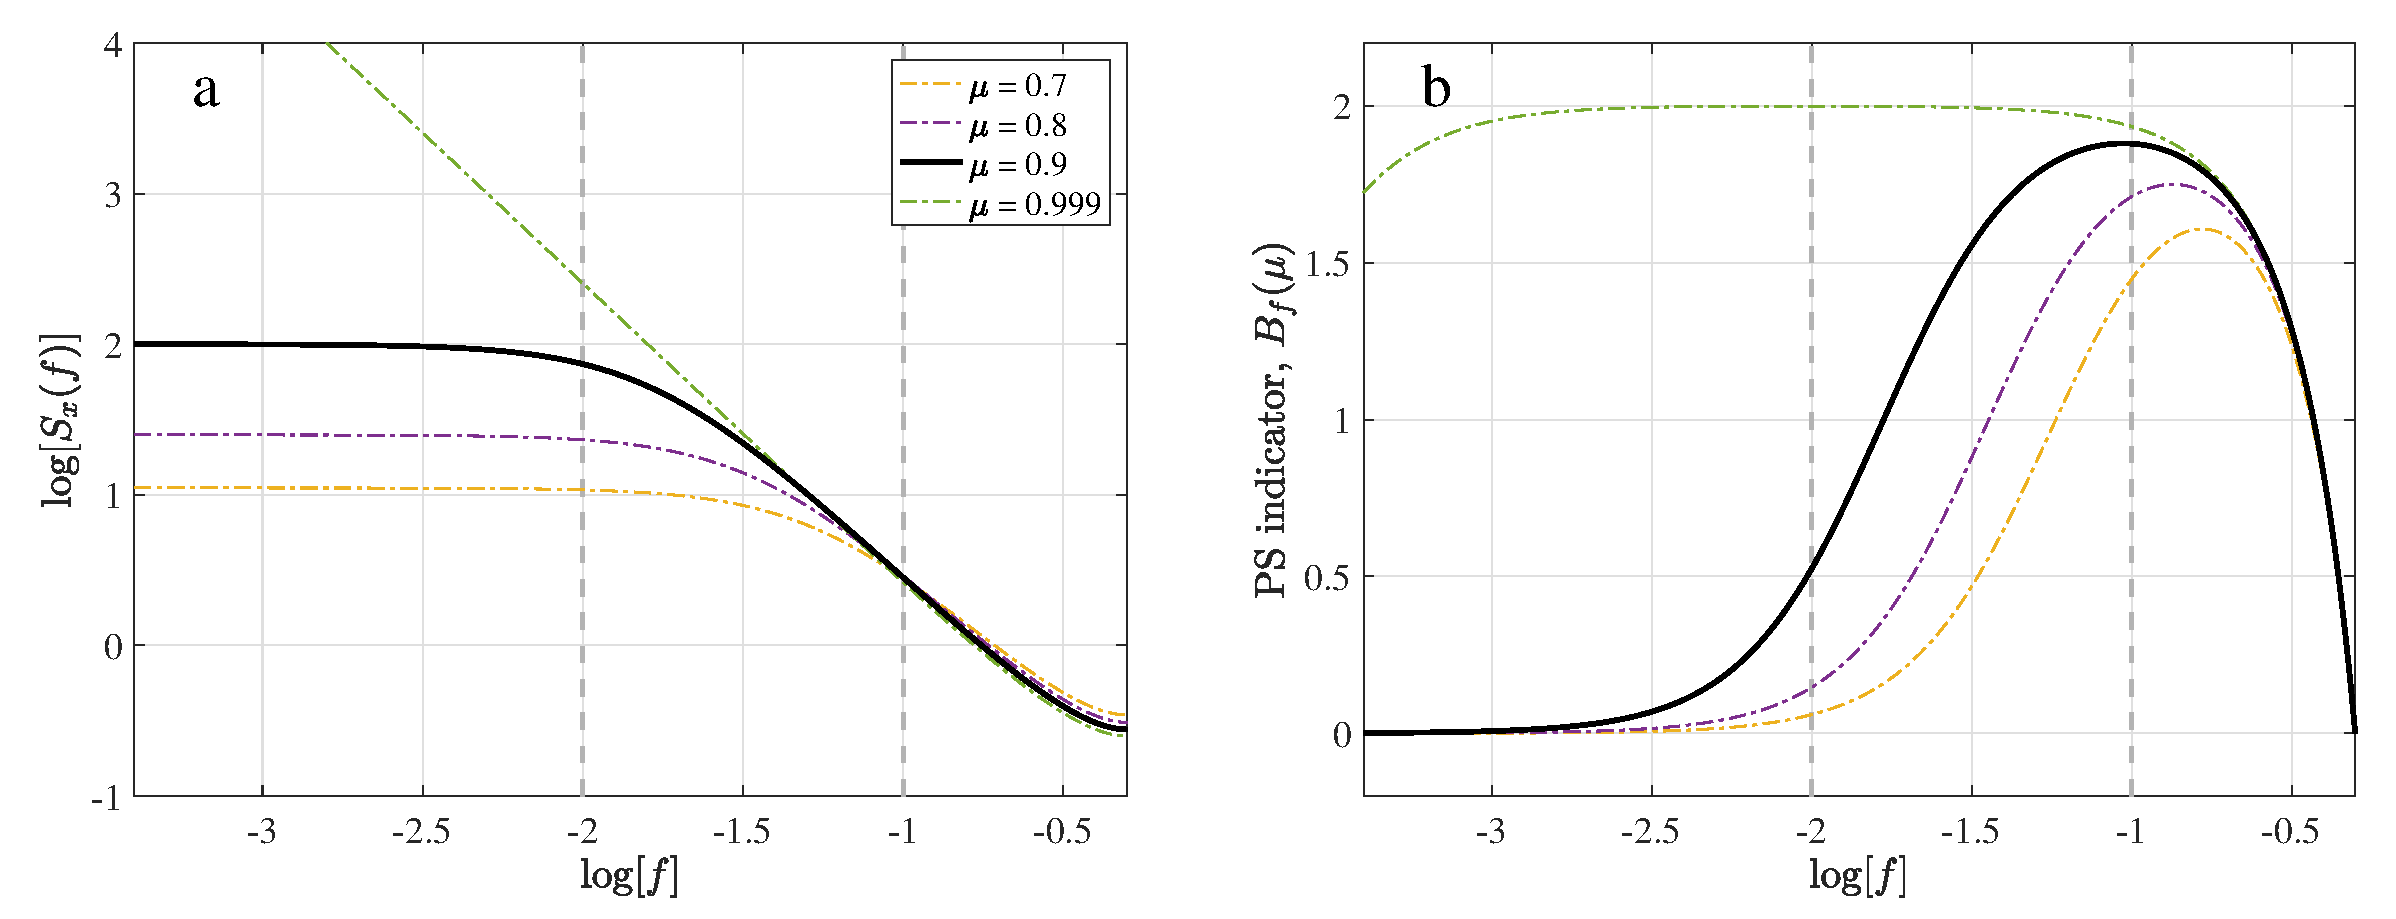
\includegraphics[width=0.9\linewidth]{AR1_powerspectrum}
	\caption{\Red{ Panel {\bf a}: The power spectrum of the AR(1) process (see equation~\ref{eqn:1D:AR1process_powerspectrum}) is plotted on a log-log scale for various values of the parameter $\mu$. Note the `white-noise' (flat) part of the power spectrum for small $f$ and the 'red-noise' (negative gradient) part for large $f$. Panel {\bf b}: The PS indicator (see equation~\ref{eqn:1D:AR1_psindicator}) is plotted as a function of $f$ for the same $\mu$ values. }}
	\label{fig:1D:AR1_powerspectrum}
\end{figure}

{\Red
In figure~\ref{fig:1D:AR1_powerspectrum} the power spectrum of the AR(1) process is plotted (panel {\bf a}) for parameter value $\mu = 0.9$. We note that for small values of $f$ ($\log f<\m2.5$) the ``white noise'' (flat) aspect of the power spectrum is visible whilst for larger values ($\log f\approx \m1$) we observe a ``red noise'' (gradient $= \m2$) feature, and there is a crossover which occurs at approximately $\log f= \m2$. We also note that, similar to the example in figure~\ref{fig:1D:crossover2}, this crossover point a value of $f$ dependent on the parameter $\mu$: also plotted are the power spectra for $\mu = 0.7,~ 0.8,~ 0.999$. In figure~\ref{fig:1D:AR1_powerspectrum}b the PS exponent $B_f$ is plotted as a function of $\log f$ for the same (fixed) values of $\mu$. We are able to see the white noise part of the power spectrum ($\log f<\m2.5$) where $B_f=0$ and the peak ($B_f\approx 2$), which occurs at $\log f\approx \m1$ for $\mu = 0.9$, corresponding to the negative-gradient `red noise' aspect of the power spectrum in panel {\bf a}. This plot also allows us to visualise the observation made in equation~\ref{eqn:1D:maximumPSindicator_AR1} that for large values of $f$ ($\log f > \m1$) the PS indicator does not reach a value close to the maximum value of 2, even for $\mu$ close to 1.

\begin{figure}
	\centering
	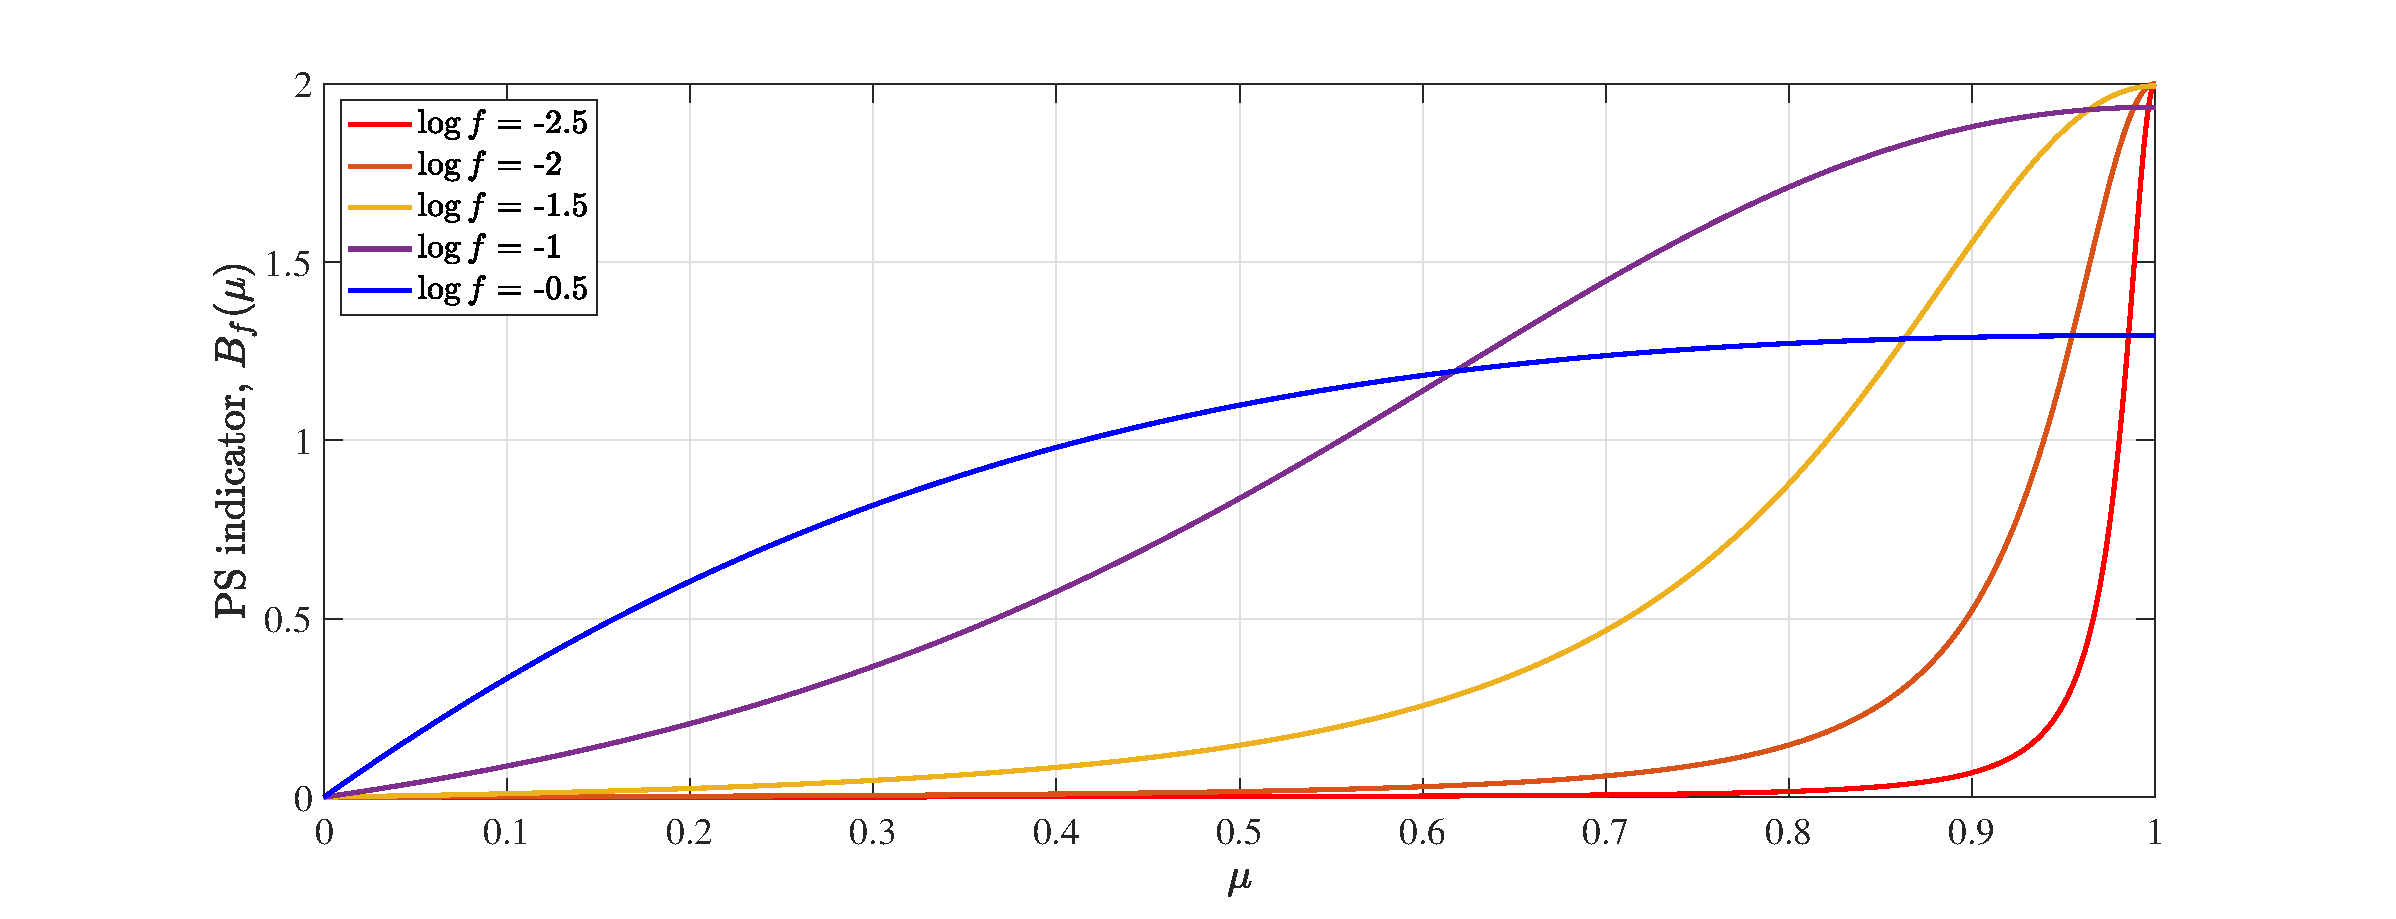
\includegraphics[width=\linewidth]{PSexponent_changingmu}
	\caption{ \Red{The PS indicator is plotted as a function of $\mu$ for various values of $f$. Note that for larger $f$ the PS indicator has a maximum value $<2$ while for smaller $f$ the indicator shows the characteristic increasing ('reddening') trend only in the $\mu>0.9$ range.}}
	\label{fig:1D:PSexponent_changingmu}
\end{figure}

In figure~\ref{fig:1D:PSexponent_changingmu} we plot the PS indicator (equation~\ref{eqn:1D:AR1_psindicator}) as a function of $\mu$ rather than as a function of time, which is equivalent to the assumption $\mu(t)=t$. The PS indicator increases, as expected, as $\mu$ increases from 0 to 1. We note that for very small values of $f$ ($\log f<\m2$) the indicator value is close to zero until the point $\mu=0.9$ when it increases very steeply. This effect can also been seen in figure~\ref{fig:1D:AR1_powerspectrum}b where we observe that even at $\mu=0.9$ the indicator is zero for small $f$, whereas for $\mu = 0.999$ the indicator is $\approx 2$ over the whole range $\m3<\log f<\m1$.  For larger $f$ it is possible to see the increasing trend in the indicator over the whole series of increasing $\mu$. For this reason, when one wishes to detect a `reddening' of noise due to critical slowing down, which is modelled as an AR(1) process \citep{ashwin2012}, the most obvious trend will be visible when measuring the PS scaling exponent using a frequency $\log f\geq\m2$. We note, however, that this will not be true if a relatively high base-level PS indicator ($B_f>0.5$) is observed for $\log f=\m2$, implying an AR(1) parameter $\mu>0.9$. In this case it may be more instructive to observe whether there is a steep increase in the indicator as $\mu$ increases between 0.9 and 1; this is clearly visible for $\log f=\m3$ but not for $\log f=\m1$. 

In practical applications where only short time series are available and the power spectrum is approximated by the fast Fourier transform periodogram, there may be very few data available in the lower frequencies due to the logarithmic scale. In these cases it may not be possible to reasonably estimate the PS exponent for small values of $f$ and so the frequencies used will be informed by the length of the time series. In table~\ref{tab:1D:AR1_frequencyrange} we have enumerated the number of data points in different frequency ranges having obtained the fast Fourier transform periodogram from a time series of $10^4$, $10^3$ and $10^2$ points. When using very short time series, say $100$ points, it is already impossible to estimate the gradient of the periodogram for frequencies $\log f<\m2$ because there are simply not enough data to perform a linear fit. However, in the range $\m2\leq\log f\leq\m1$ it is at least possible, with 10 points available, although we note that this will likely give a very noisy PS indicator and longer time series or large ensembles would be preferred.

\begin{table}
	\centering
	\begin{tabular}{ c c  c  c }
		\hline
		\multirow{2}{*}{Frequency range} & \multicolumn{3}{c}{Number of data in range}\\
		& $N=10^{4}$ & $N=10^{3}$ & $N=10^{2}$\\
		\hline \hline
		$\m3.5\leq\log f\leq\m2.5$ & 28   & 3   & 0\\
		$\m3\leq\log f\leq\m2$     & 91   & 10  & 1\\
		$\m2.5\leq\log f\leq\m1.5$ & 285  & 28  & 3\\
		$\m2\leq\log f\leq\m1$     & 901  & 91  & 10\\
		$\m1.5\leq\log f\leq\m0.5$ & 2846 & 285 & 28\\
		\hline
	\end{tabular}
	\caption{\Red{The fast Fourier transform periodogram is obtained for time series of length $10^4$, $10^3$ and $10^2$ and the number of data in various frequency ranges is recorded. For time series of length $10^2$ there are not sufficient data to estimate the PS scaling exponent for $\log f<\m2$.}}
	\label{tab:1D:AR1_frequencyrange}
\end{table}

Taking all of these factors into account, we conclude that using a frequency range $\m2\leq\log f\leq\m1$ in which to measure the PS scaling exponent will give the most clearly observable increase in the PS indicator during critical slowing down. At the higher end of this range we begin to observe the sudden drop in the maximum exponent value; at the lower end of the range there exist the dual problems of almost no increase for parameter values below $\mu=0.9$, and an insufficient number of data for estimation when dealing with short time series.

}


\subsection{Sensitivity of PS indicator to window size}
\label{subsec:1D:Exponents_as_EWS:PSsensitivity}
{\Red{
		In section~\ref{subsec:1D:Exponents_as_EWS:indicators}, where the PS indicator is introduced, we have remarked that by calculating the PS exponent $\beta$ of an AR(1) time series in the frequency range $\m1\leq\log_{10} f\leq\m2$ we can reconstruct the parameter $\mu$ of the AR(1) since the two are related via equation~\ref{eqn:1D:PSindicator:reconstruct_mu}, that is, 
		\begin{equation}
		\label{eqn:1D:PSindicator:reconstruct_mu_repro}
		\mu\approx b-\sqrt{b^2-1}~~~\text{where}~~~ b = \frac{\cos(0.2\pi)-10^\beta \cos(0.02\pi)}{1-10^\beta}.
		\end{equation}
		The numerical verification of this derived equation is presented in figure~\ref{fig:1D:PSofAR1} (page~\pageref{fig:1D:PSofAR1}), where we demonstrate that the analytic relationship between $\mu$	and $\beta$ is approximately the same as the relationship between the PS exponent and the lag-1 autocorrelation calculated for a set of AR(1) time series with parameter $\mu\in[0,1]$. This verification, however, used AR(1) time series of length $10^5$, and would only be a valid test of the PS indicator if a window size of $10^5$ were used. This is clearly not always possible in practical situations and, if it were, might anyway be computationally expensive. 
		
		The selection of the window size when calculating an EWS indicator in a sliding window is always a compromise which takes into account the nature of the time series data, the time scale of the tipping event to be detected or predicted, and the error in the EWS. A very short window size will typically contain more error in the indicator calculation, whilst a very large window size will smooth out the effect upon the indicator of the tipping event, or may be prevented by only a short time series being available for analysis. In order to investigate further the limitations of using a small window size, the numerical results presented in figure~\ref{fig:1D:PSofAR1} are examined in more detail here, this time using a range of different lengths of the AR(1) time series. 
		
		For a range of `series lengths' between $10^2$ and $10^5$, one hundred time series are produced from an AR(1) process with parameter in the range $0\leq\mu\leq1$. For each of these time series the value of $\mu$ is estimated using two different methods: by calculating the PS exponent and using the formula in equation~\ref{eqn:1D:PSindicator:reconstruct_mu_repro}, or simply by calculating the lag-1 autocorrelation (ACF1). In each case, the difference between this estimated value and the real value of $\mu$ is found simply as $|\mu-\mu_\text{est}|$ and the mean of these differences is taken over the $100$ values of $\mu$ to give a single-value measure of the error inherent in each method for each series length.
		
		In fact equation~\ref{eqn:1D:PSindicator:reconstruct_mu_repro} is only valid for $0<\mu\leq1$, or equivalently $0<\beta\leq1.985$. When estimating the parameter $\mu$ we therefore impose the piece-wise condition
		\begin{equation}
			\mu_\text{est} = \begin{cases}
			0&~\text{if}~\beta\leq0\\
			b-\sqrt{b^2-1}&~\text{if}~0<\beta\leq1.985\\
			1&~\text{if}~\beta>1.9850
			\end{cases}
		\end{equation}
		where $b$ is given as in equation~\ref{eqn:1D:PSindicator:reconstruct_mu_repro}. In applications of the PS indicator to tipping points we are interested in the value of the PS indicator itself as a proxy for `reddening' noise in a time series and we do not literally estimate the AR(1) model parameter in this way. For the purpose of comparison, however, this is a useful exercise. 
		
		The results of this exercise are presented in figure~\ref{fig:1D:PSsensitivity}a whilst the individual results for the time series of length $10^2$ (the shortest considered) and length $10^5$ (the longest considered) are shown in figures figure~\ref{fig:1D:PSsensitivity}b,c. We note (in panel {\bf a}) that the error is always larger in the power spectrum approach than in the autocorrelation approach and that whilst the error in each method is larger for short series lengths, so the difference between the two methods is also larger. 
	}}



\begin{figure}
	% plotted using the Matlab script 'PSwindowsize_sensitivity.m'
	\centering
	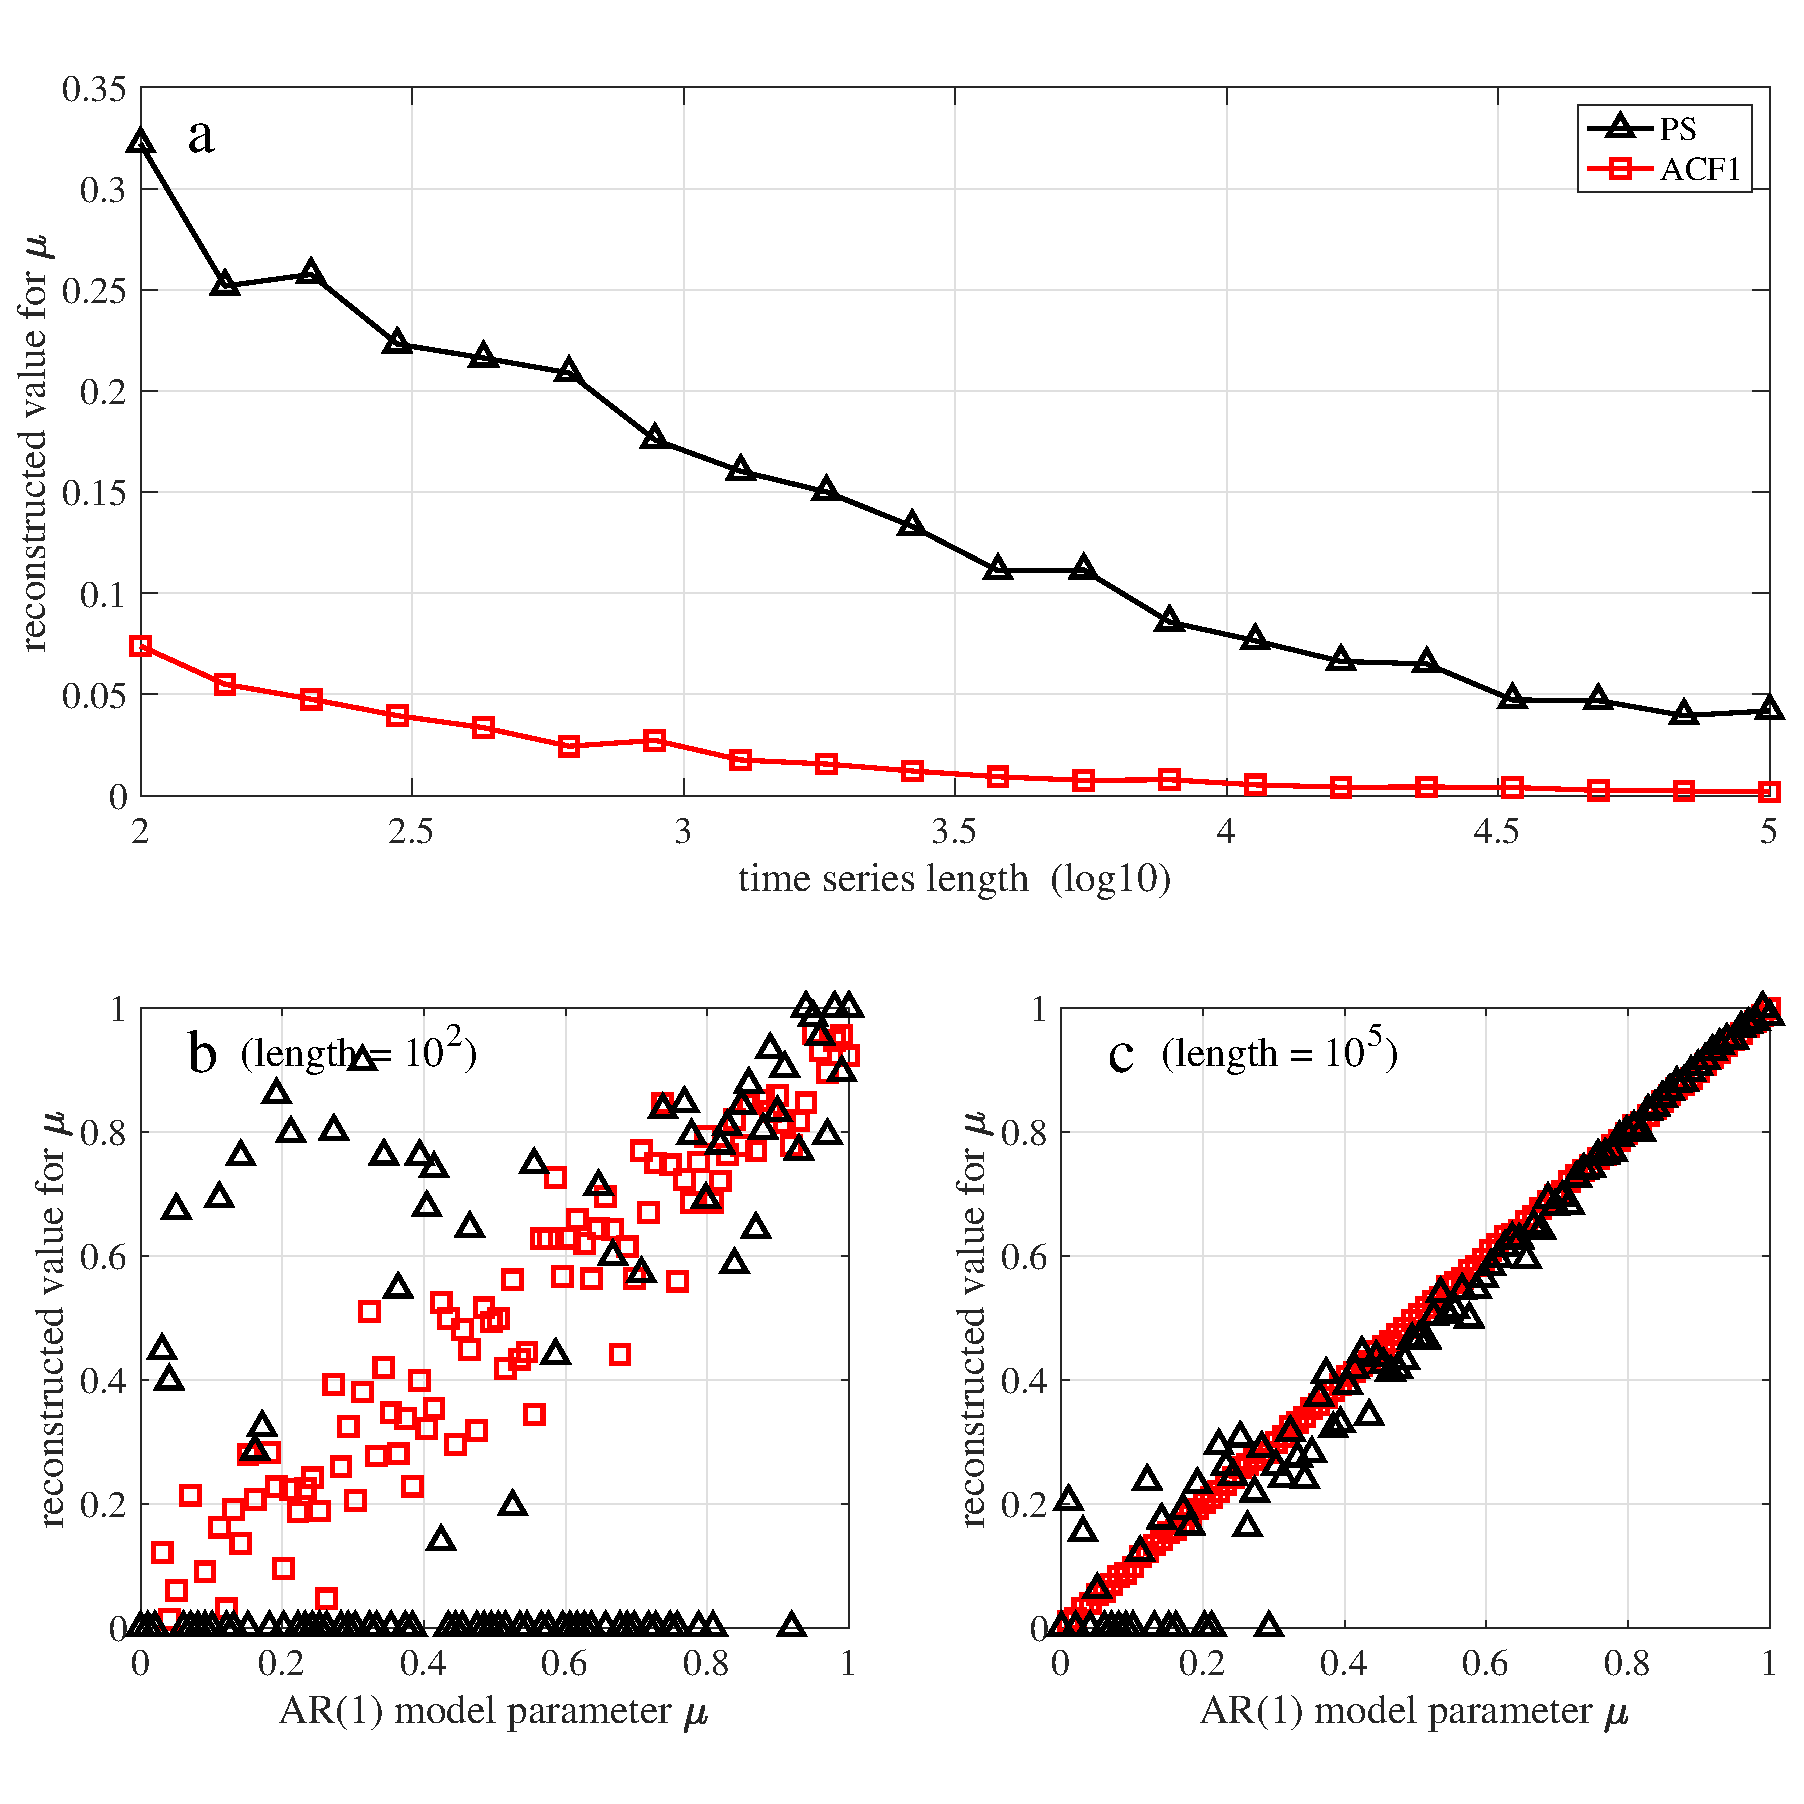
\includegraphics[width=0.9\linewidth]{PSwindowsize_sensitivity_1e5}
	\caption{\label{fig:1D:PSsensitivity}
		\Red{Panel {\bf a}: For $10^2\leq N\leq 10^5$ time series of length $N$ are created using an AR(1) model with $100$ different values of the parameter $\mu$ in the range $[0,1]$. The value of the model parameter is then estimated using either the lag-1 autocorrelation or the PS exponent $\beta$ (see equation~\ref{eqn:1D:PSindicator:reconstruct_mu_repro}). The mean difference between the estimated value and the true value is plotted for the ACF1 method (red squares) and the PS method (black triangles).  Panels {\bf b}, {\bf c}: The estimated values of the parameter $\mu_{\text{est}}$ are plotted against the true values $\mu$ when using a series length $N=10^2$ (the shortest considered) and $10^5$ (the longest considered). }
	}
\end{figure}

{\Red{
		Whilst it is clear that the ACF1 method out-performs the PS method for every time series length, we note that in both the short series (length $N=10^2$) and the long series (length $N=10^5$) the PS method is better at estimating the true value of $\mu$ for higher values of $\mu$ than it is for lower values. In figure~\ref{fig:1D:PSsensitivity}b ($N=10^2$) we note that whilst the estimated value is extremely variable for low values of $\mu$ it is reasonably close to the true value for $\mu>0.8$. In figure~\ref{fig:1D:PSsensitivity2} we replot the same data as figure~\ref{fig:1D:PSsensitivity}a, but only considering either small values $\mu\leq0.4$ (top panel) or large values $\mu\geq0.6$ (bottom panel). We note the improved accuracy of the PS method when considering only large values of $\mu$, particularly for series length $N>10^3$. This is to be expected somewhat if we consider the shape of the function that relates $\mu$ and $\beta$ which has been used in this experiment. The value of $\beta$ as a function of $\mu$ is shown in figure~\ref{fig:1D:PSofAR1}, the formula given by equation~\ref{eqn:1D:PSindicator:reconstruct_mu_repro} is simply the inverse function. We see in this that for small $\mu$ a large change in $\mu$ gives only a small change in $\beta$, whereas this is the opposite for large $\mu$. We can therefore expect that, when $\mu$ is small, a small error in the estimation of the PS exponent $\beta$ will translate into a much larger error in the estimated value of $\mu$ using the formula in equation~\ref{eqn:1D:PSindicator:reconstruct_mu_repro}. When using the PS indicator we bear in mind that it is used as a proxy for the `reddening' of noise over time which is caused by critical slowing down, not to provide an accurate parametrisation of an AR(1) model. Also, the increase in the AR(1) parameter which is expected in the presence of critical slowing down is not necessarily linear, and so the non-linear relationship between $\mu$ and $\beta$ (which is here responsible for the error at low values of $\mu$) may not necessarily be a problem, depending on the application.
}}

\begin{figure}
	% plotted using the Matlab script 'PSwindowsize_sensitivity.m'
	\centering
	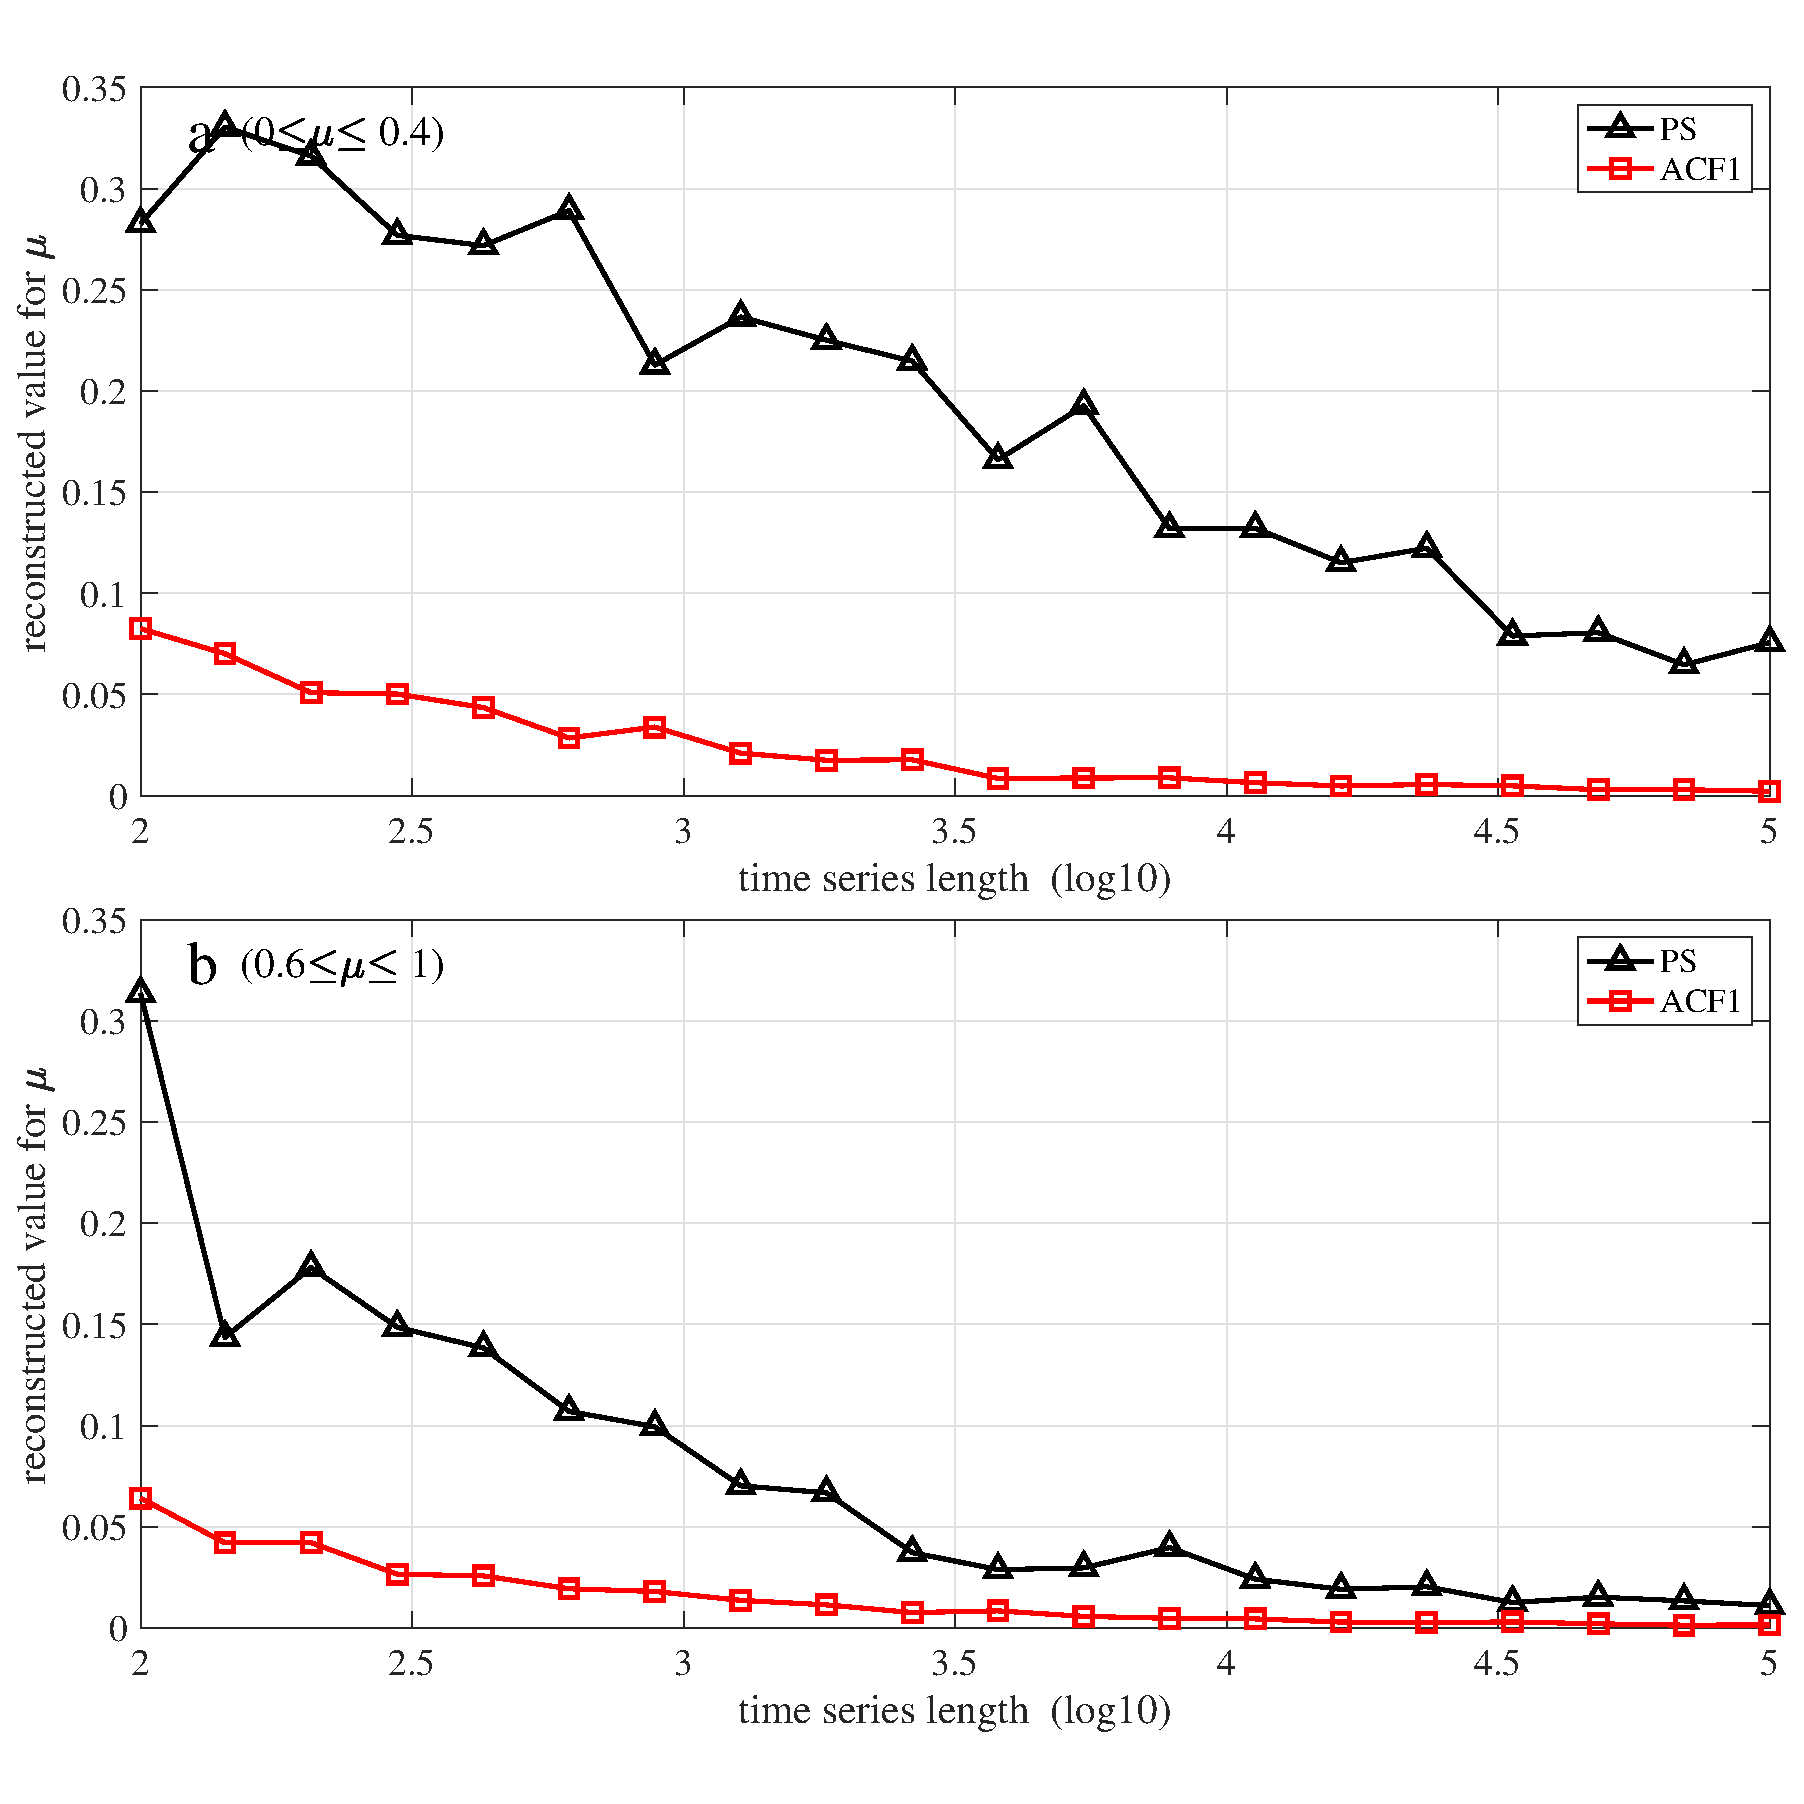
\includegraphics[width=0.9\linewidth]{PSwindowsize_sensitivity_BigAndSmall_1e5}
	\caption{\label{fig:1D:PSsensitivity2}
		\Red{For $10^2\leq N\leq 10^5$ time series of length $N$ are created using an AR(1) model with $100$ different values of the parameter $\mu$. The value of the model parameter is then estimated using either the lag-1 autocorrelation or the PS exponent $\beta$ (see equation~\ref{eqn:1D:PSindicator:reconstruct_mu_repro}). The mean difference between the estimated value and the true value is plotted for the ACF1 method (red squares) and the PS method (black triangles). Panel {\bf a} shows the result of the experiment for $\mu$ in the range $[0, 0.4]$ (small $\mu$) whilst panel {\bf b} shows the result of the experiment for $\mu$ in the range $[0.6, 1]$ (large $\mu$). }
	}
\end{figure}

{\Red{
		In figure~\ref{fig:1D:PSsensitivity_trend} we show the results of this experiment repeated but instead of a simple AR(1) model, a parabolic trend has been superimposed onto the resulting times series. For each different value of the series length $N$, a time series is produced using
		\begin{equation}
			X(t_{n}) = \mu X(t_{n-1}) + \eta_n + 5t_n^2\,,
		\end{equation} 
		where $[t_1,\dots,t_N] = [0,\dots,1]$ and the $\eta_n$ are independent Gaussian white noise terms. We expect that by introducing non-stationarity in this way the auto-correlation of the time series will increase and tend to make any estimate of the parameter $\mu$ an \emph{over}-estimate. In figure~\ref{fig:1D:PSsensitivity_trend}b we see that this is indeed the case where the series length is $N=10^2$: both estimated parameters are much closer to $1$ than to the true value, although the estimate obtained from the PS method (black triangles) appears to be random whilst the values obtained using the ACF1 method follow a linear pattern, whilst being consistently higher than the true values. For longer series lengths, however, this is not the case. In figure~\ref{fig:1D:PSsensitivity_trend}c, where the series length is $N=10^5$, the estimated values obtained using ACF1 follow the same linear relationship to the true values as they did for smaller $N$. The values obtained using the PS method are, however, in agreement with the true values, especially closely for the larger values of $\mu$. It appears that estimating the AR(1) model parameter using the PS exponent is not affected by whether there is or is not a trend superimposed on the AR(1) process time series, at least when the time series is sufficiently long. 
		
		In the context of providing early warning signals it is, of course, not the value of the indicator that is important but the trend in the indicator over time. In light of this, it is not necessarily a problem that the ACF1 indicator is biased by the trend in the time series, but in cases where trends in the time series are not predictable this bias could cause misleading trends to appear in the ACF1 indicator series. This bias may be overcome by first detrending each segment of the time series in which the indicator value is calculated, which is similar in principle to the detrending step in the DFA algorithm \citep{kantelhardt2001, livina2007}. For long time series, or long window sizes, the PS indicator calculation may provide the benefit of not requiring the detrending step, which may in fact introduce new inaccuracies if the detrending is of the wrong order. 
				
	}}

\begin{figure}
	% plotted using the Matlab script 'PSwindowsize_sensitivity.m'
	\centering
	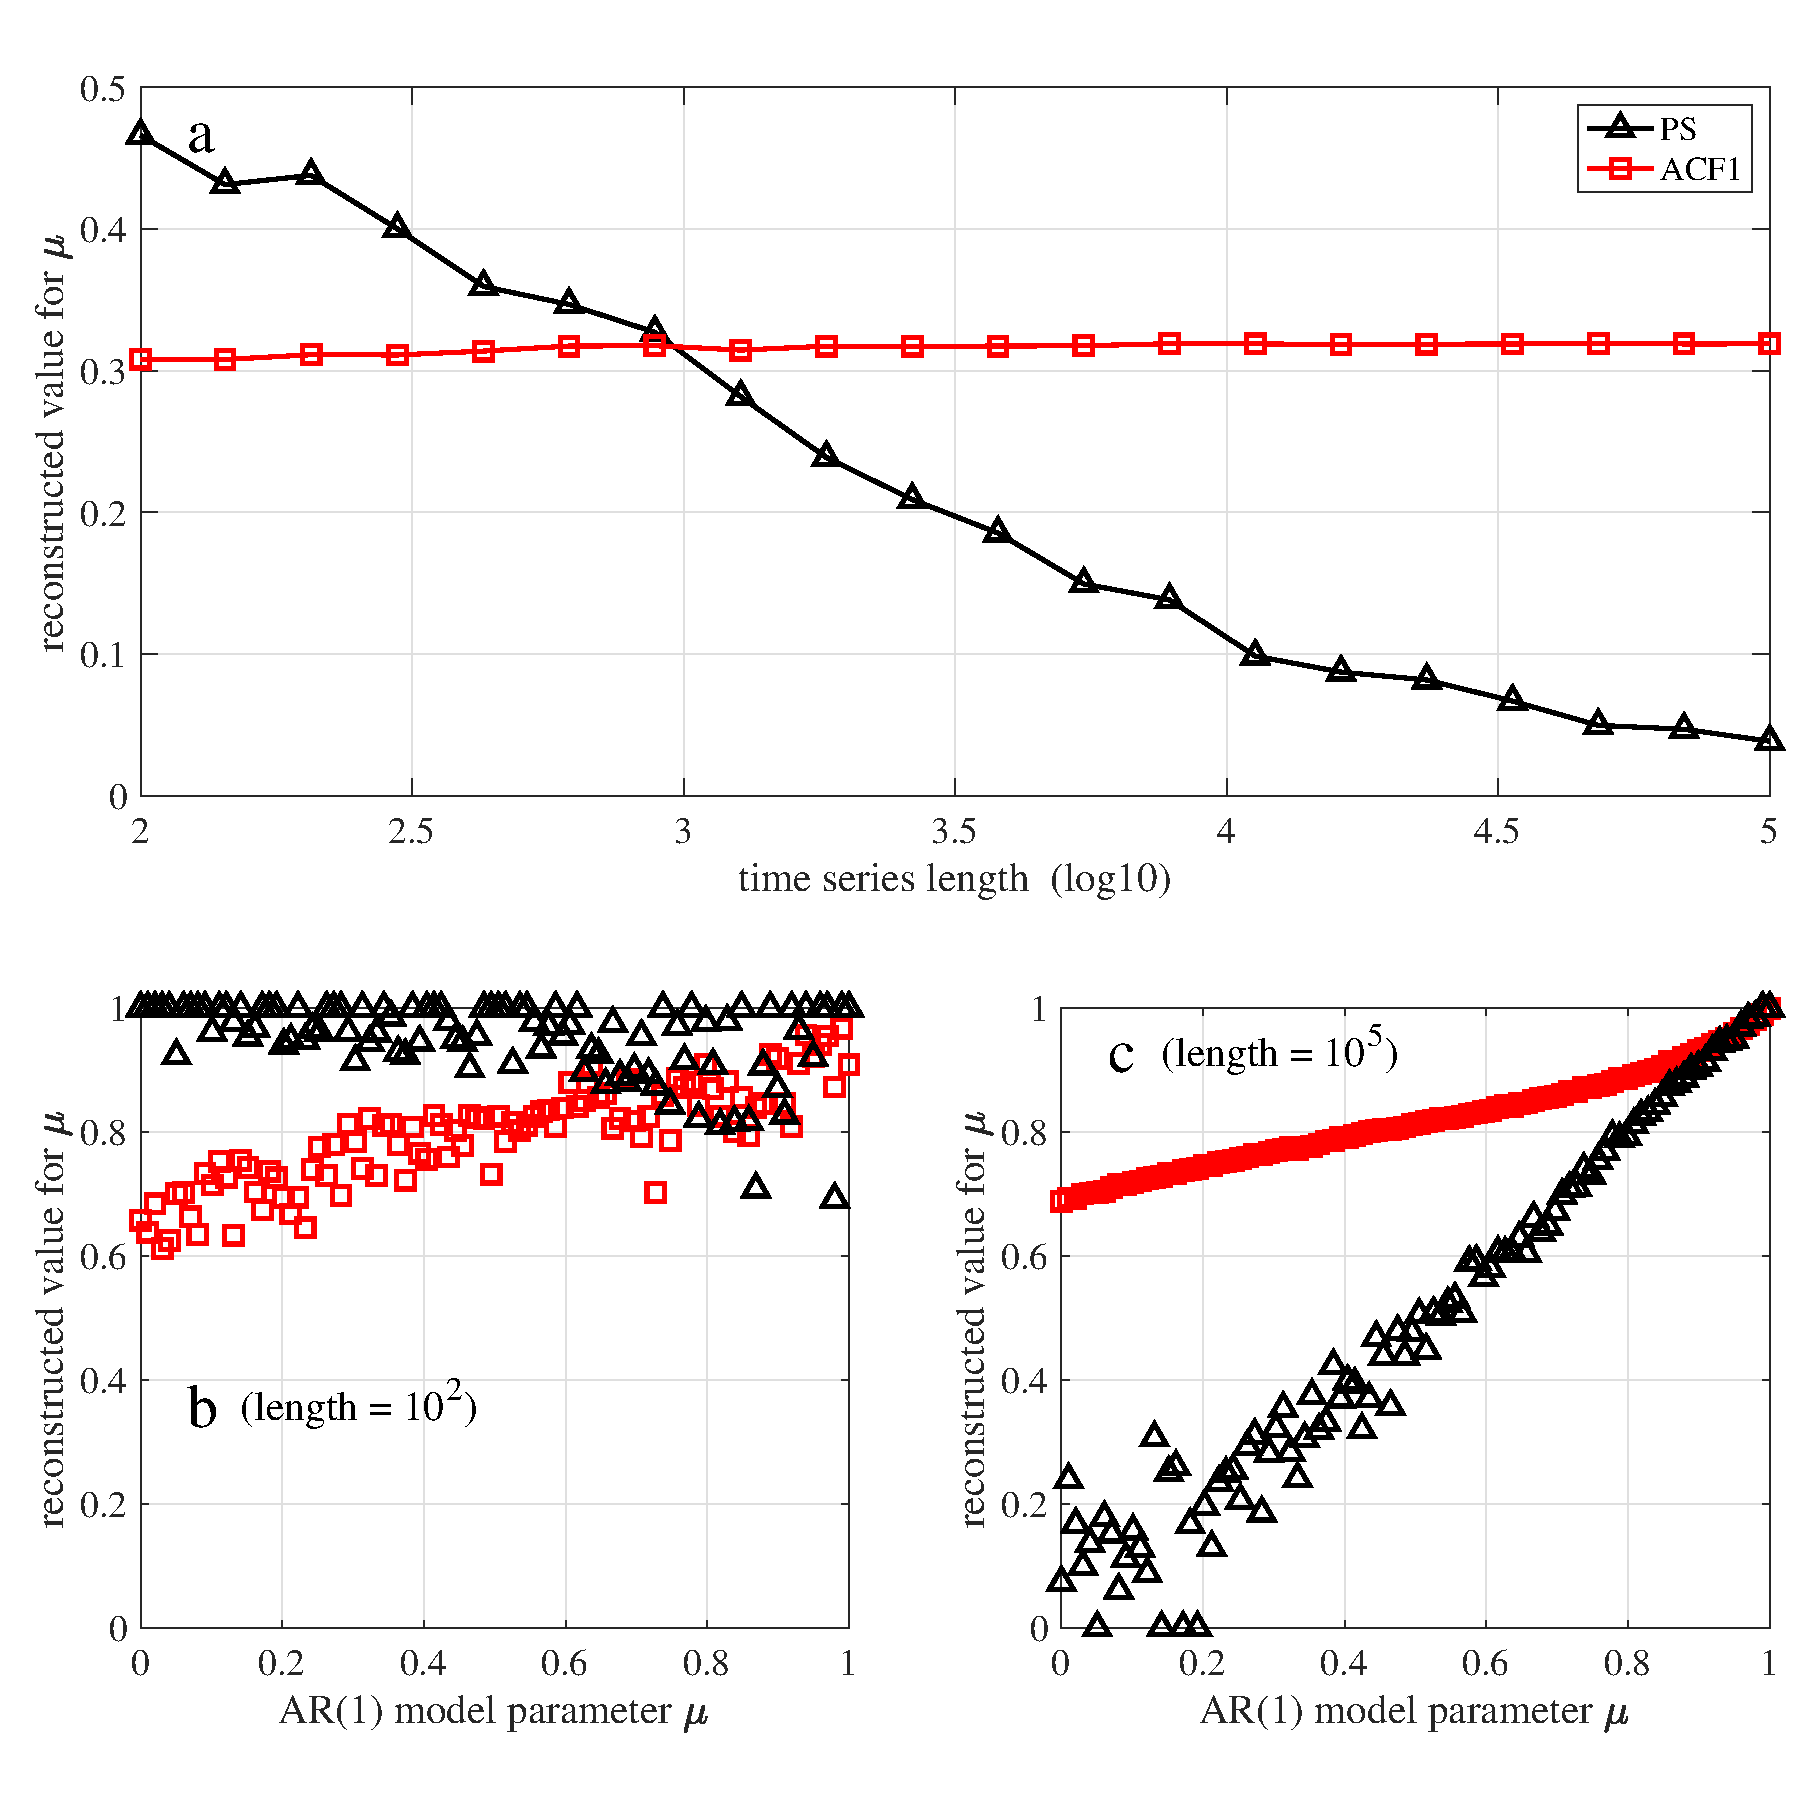
\includegraphics[width=0.9\linewidth]{PSwindowsize_sensitivity_trend}
	\caption{\label{fig:1D:PSsensitivity_trend}
		\Red{[Repeat of the experiment in figure~\ref{fig:1D:PSsensitivity} but the AR(1) model has a superimposed parabolic trend] Panel {\bf a}: For $10^2\leq N\leq 10^5$ time series of length $N$ are created using an AR(1) model with a parabolic trend with $100$ different values of the parameter $\mu$ in the range $[0,1]$. The value of the model parameter is then estimated using either the lag-1 autocorrelation or the PS exponent $\beta$ (see equation~\ref{eqn:1D:PSindicator:reconstruct_mu_repro}). The mean difference between the estimated value and the true value is plotted for the ACF1 method (red squares) and the PS method (black triangles).  Panels {\bf b}, {\bf c}: The estimated values of the parameter $\mu_{\text{est}}$ are plotted against the true values $\mu$ when using a series length $N=10^2$ (the shortest considered) and $10^5$ (the longest considered). }
	}
\end{figure}

\subsection{Parametrising an AR(1) process with non-constant parameter}
\label{subsec:1D:Exponents_as_EWS:PSnonstationary}
{\Red{
		All of the results in section~\ref{subsec:1D:Exponents_as_EWS:PSsensitivity} use time series from an AR(1) process $x(t_n) = \mu x(t_{n-1})+\eta_n$ where $\mu$ is constant. Indeed, the work in section~\ref{subsec:1D:Exponents_as_EWS:determining_frequency_range}, where we determine the frequency range in which to estimate the PS exponent assumes a constant $\mu$ and relies on the equation for the power spectrum of such an AR(1) process (see equation~\ref{eqn:1D:PSindicator:AR1powerspectrum}, page~\pageref{eqn:1D:PSindicator:AR1powerspectrum}). Of course, in applications of the PS indicator, or any indicator, to obtain an early warning signal, such stationarity cannot be assumed. Indeed, the very purpose of using these indicators is to detect an \emph{increase} in the `redness' due to critical slowing down, for which the AR(1) parametrisation is a proxy. 
		
		In practice we apply the early warning indicators to time series of dynamical systems with constantly changing parameters, and therefore within each time window the parameters will also be changing. In this case the PS scaling exponent or the lag-1 autocorrelation is calculated for this window of the time series and the result is provide a single-value measure representing the shape of the power spectrum in that window. Taking the single-parameter AR(1) model as an example, we might desire that the estimated value $\mu_\text{est}$ obtained using these methods is equal to the mean value of parameter $\mu$ in that window, which would produce consistent results if the rate of change of $\mu$ was non-constant. 
		
		We consider a modified AR(1) process
		\begin{equation}
			\label{eqn:1D:AR1process_changingparameter}
			x(t_n) = \mu_n x(t_{n-1})+\eta_n
		\end{equation}
		where the $\mu_n$ increase linearly in some interval $[\mu_0, \mu_N]$. If we calculate the PS exponent or lag-1 autocorrelation of this process we desire that the result is the same as it would be for a normal AR(1) process with constant parameter $\mu=(\mu_0+\mu_N)/2$ the mean value of the changing parameter. We test this hypothesis experimentally by partitioning the interval $[0,1]$ into $30$ overlapping segments of length $0.2$, so that the first segment is the interval $[0,0.2]$, etc.. For each segment we construct a length $N=10^5$ time series of an AR(1) process with $\mu$ increasing, as in equation~\ref{eqn:1D:AR1process_changingparameter}, within the interval defined by that segment. The PS exponent $\beta$ is then calculated for that time series, as is the lag-1 autocorrelation. 
		
		The results of this experiment are shown in figure~\ref{fig:1D:PS_nonstationary}. The intervals over which $\mu$ increases in each time series is plotted as a horizontal line, with the midpoint marked by a circle. The grey line shows the expected relationship between an AR(1) parameter and either the PS exponent (panel {\bf a}) or the lag-1 autocorrelation (panel {\bf b}). We note that in both cases the midpoint of the interval is close to the value that would be expected if using a constant-parameter AR(1) process with that midpoint as the parameter. We are able to conclude then that for the modified AR(1) process of equation~\ref{eqn:1D:AR1process_changingparameter}, when $\mu$ is increasing linearly, the PS indicator and ACF1 indicator can be expected to provide consistent results. 
		
		In figure~\ref{fig:1D:PS_nonstationary_BigMu} we look more closely at this effect for only values of $\mu$ greater than $0.6$, this time using a segment size of $0.1$ rather than $0.2$, and we note that the results are much the same, although the difference between the calculated value at the midpoints (circles) and the true values (grey line) is less both for the PS exponent and the lag-1 ACF. This is to be expected since the segments are shorter and so the parameter varies less over each time series, and also we know the PS exponent estimation to be more accurate for larger values of the AR(1) parameter (see section~\ref{subsec:1D:Exponents_as_EWS:PSsensitivity}).

}}

\begin{figure}
	% plotted using the Matlab script 'PS_nonstationary.m'
	\centering
	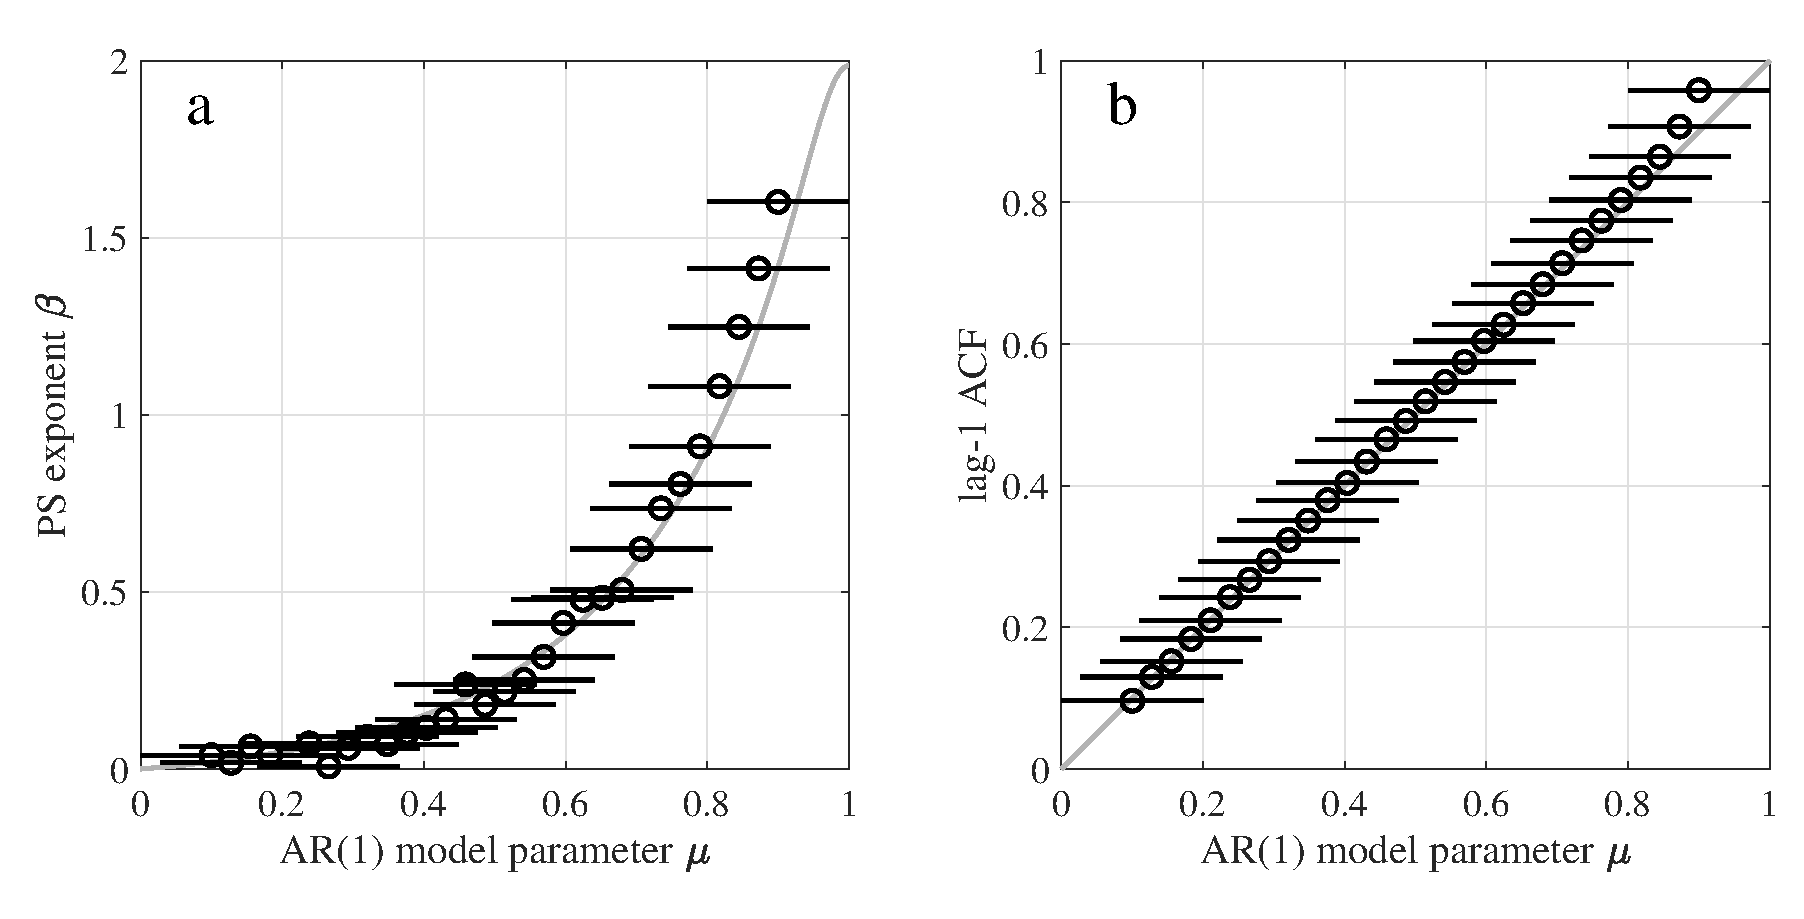
\includegraphics[width=0.9\linewidth]{PS_nonstationary}
	\caption{\label{fig:1D:PS_nonstationary}
		\Red{ $30$ time series of length $10^5$ are produced from an AR(1) process with parameter $\mu$ increasing linearly within an interval of values of length $0.2$. The PS exponent (panel {\bf a}) and the lag-1 ACF (panel {\bf b}) are calculated for each time series and the interval of $\mu$ values is plotted against the result in each case. The midpoints of the intervals are marked by circles. A grey line shows, in each case, the true value of $\beta$ or the lag-1 ACF for an AR(1) process with parameter $\mu$.}
	}
\end{figure}

\begin{figure}
	% plotted using the Matlab script 'PS_nonstationary.m'
	\centering
	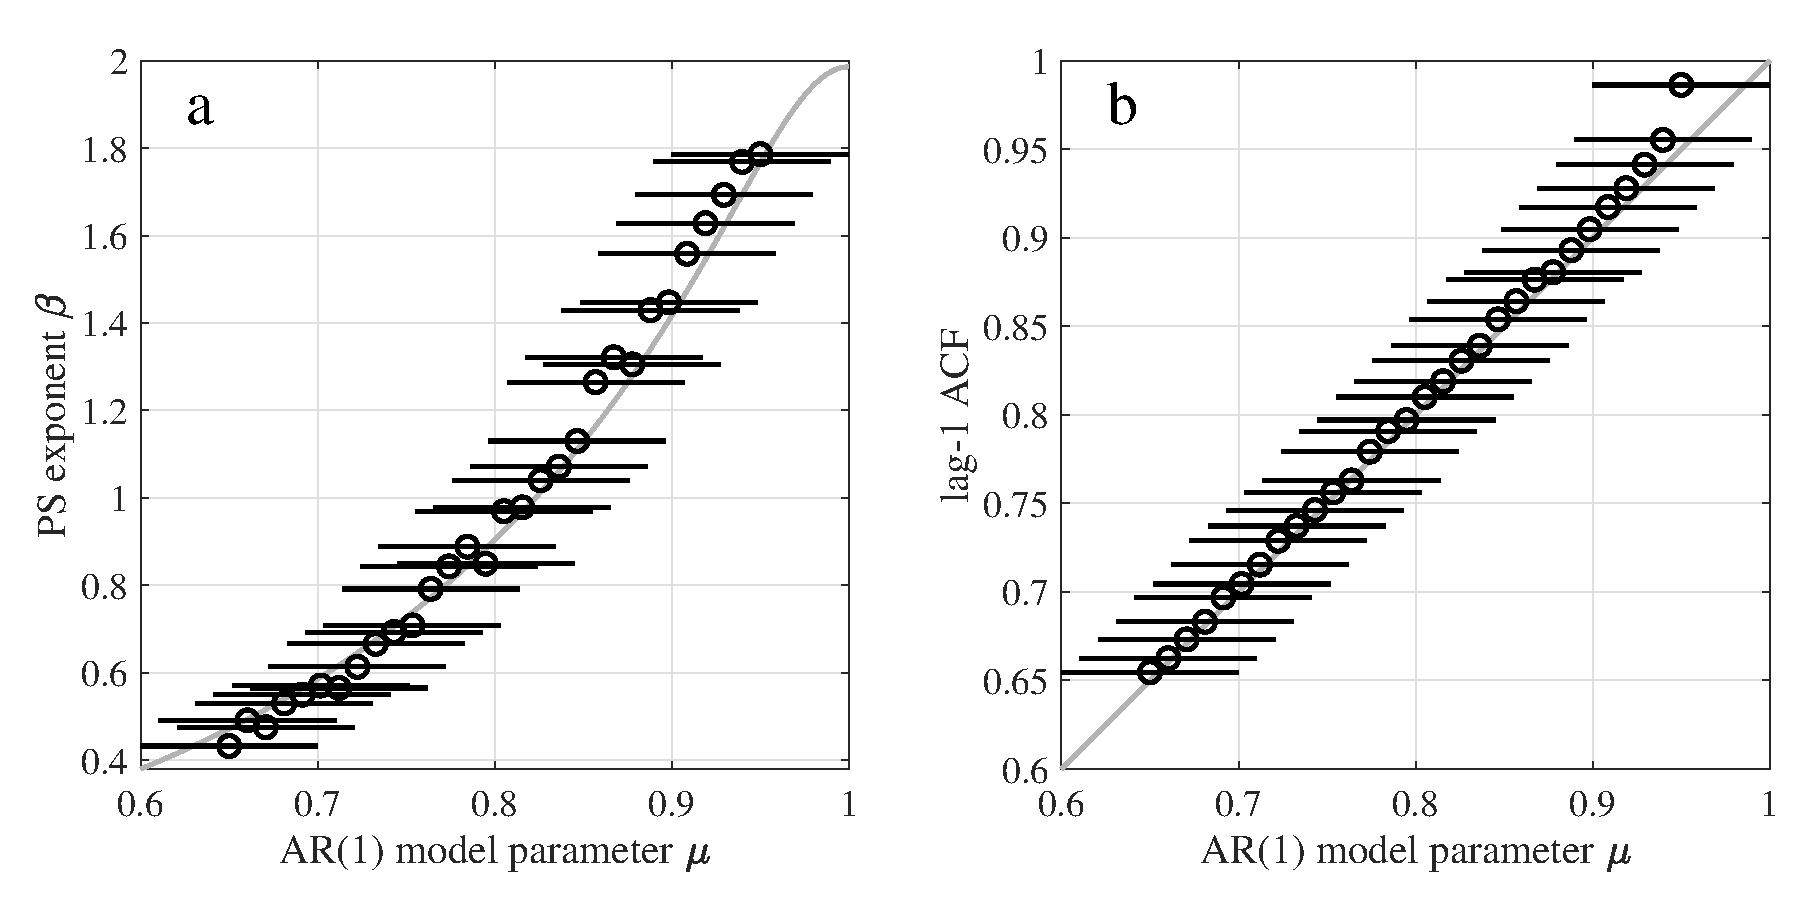
\includegraphics[width=0.9\linewidth]{PS_nonstationary_BigMu}
	\caption{\label{fig:1D:PS_nonstationary_BigMu}
		\Red{[Repeat of the experiment shown in figure~\ref{fig:1D:PS_nonstationary} but with short intervals and considering only values of $\mu$ greater than $0.6$] $30$ time series of length $10^5$ are produced from an AR(1) process with parameter $\mu$ increasing linearly within an interval of values of length $0.1$. only values $\mu\geq0.6$ are considered. The PS exponent (panel {\bf a}) and the lag-1 ACF (panel {\bf b}) are calculated for each time series and the interval of $\mu$ values is plotted against the result in each case. The midpoints of the intervals are marked by circles. A grey line shows, in each case, the true value of $\beta$ or the lag-1 ACF for an AR(1) process with parameter $\mu$.}
	}
\end{figure}

\subsection{Sensitivity of indicators to periodicity}
\label{subsec:1D:Exponents_as_EWS:Periodicity}

{\Red{
In section~\ref{subsec:1D:Exponents_as_EWS:PSsensitivity} we investigated the relationship between the parameter $\mu$ of an AR(1) process and the PS exponent $\beta$ as estimated using the periodogram. We find that for a long enough time series the PS exponent is close to the value predicted by equation~\ref{eqn:1D:PSindicator:reconstruct_mu} which is derived from the equation for the power spectrum of the AR(1) process. We also showed that for a long enough time series the PS exponent is closer to the predicted value than the lag-1 autocorrelation if a parabolic trend is superimposed onto the AR(1) process time series. 

In this section we perform a similar experiment but impose a periodic function (a sine wave) onto the time series. We expect that the PS exponent will not be much affected by this periodicity since adding a sine wave to a time series does not affect the power spectrum beyond adding a single spike at the frequency of the added wave. The PS exponent is determined by taking the linear gradient across a range of frequencies and changing one point will not significantly alter the result. Additionally, if the frequency of the sine wave is outside of the range used in the estimation of the PS exponent, it will not affect the result at all. 
}}

\begin{figure}
	% plotted using the Matlab script 'AR1plusSineWavePlot.m'
	\centering
	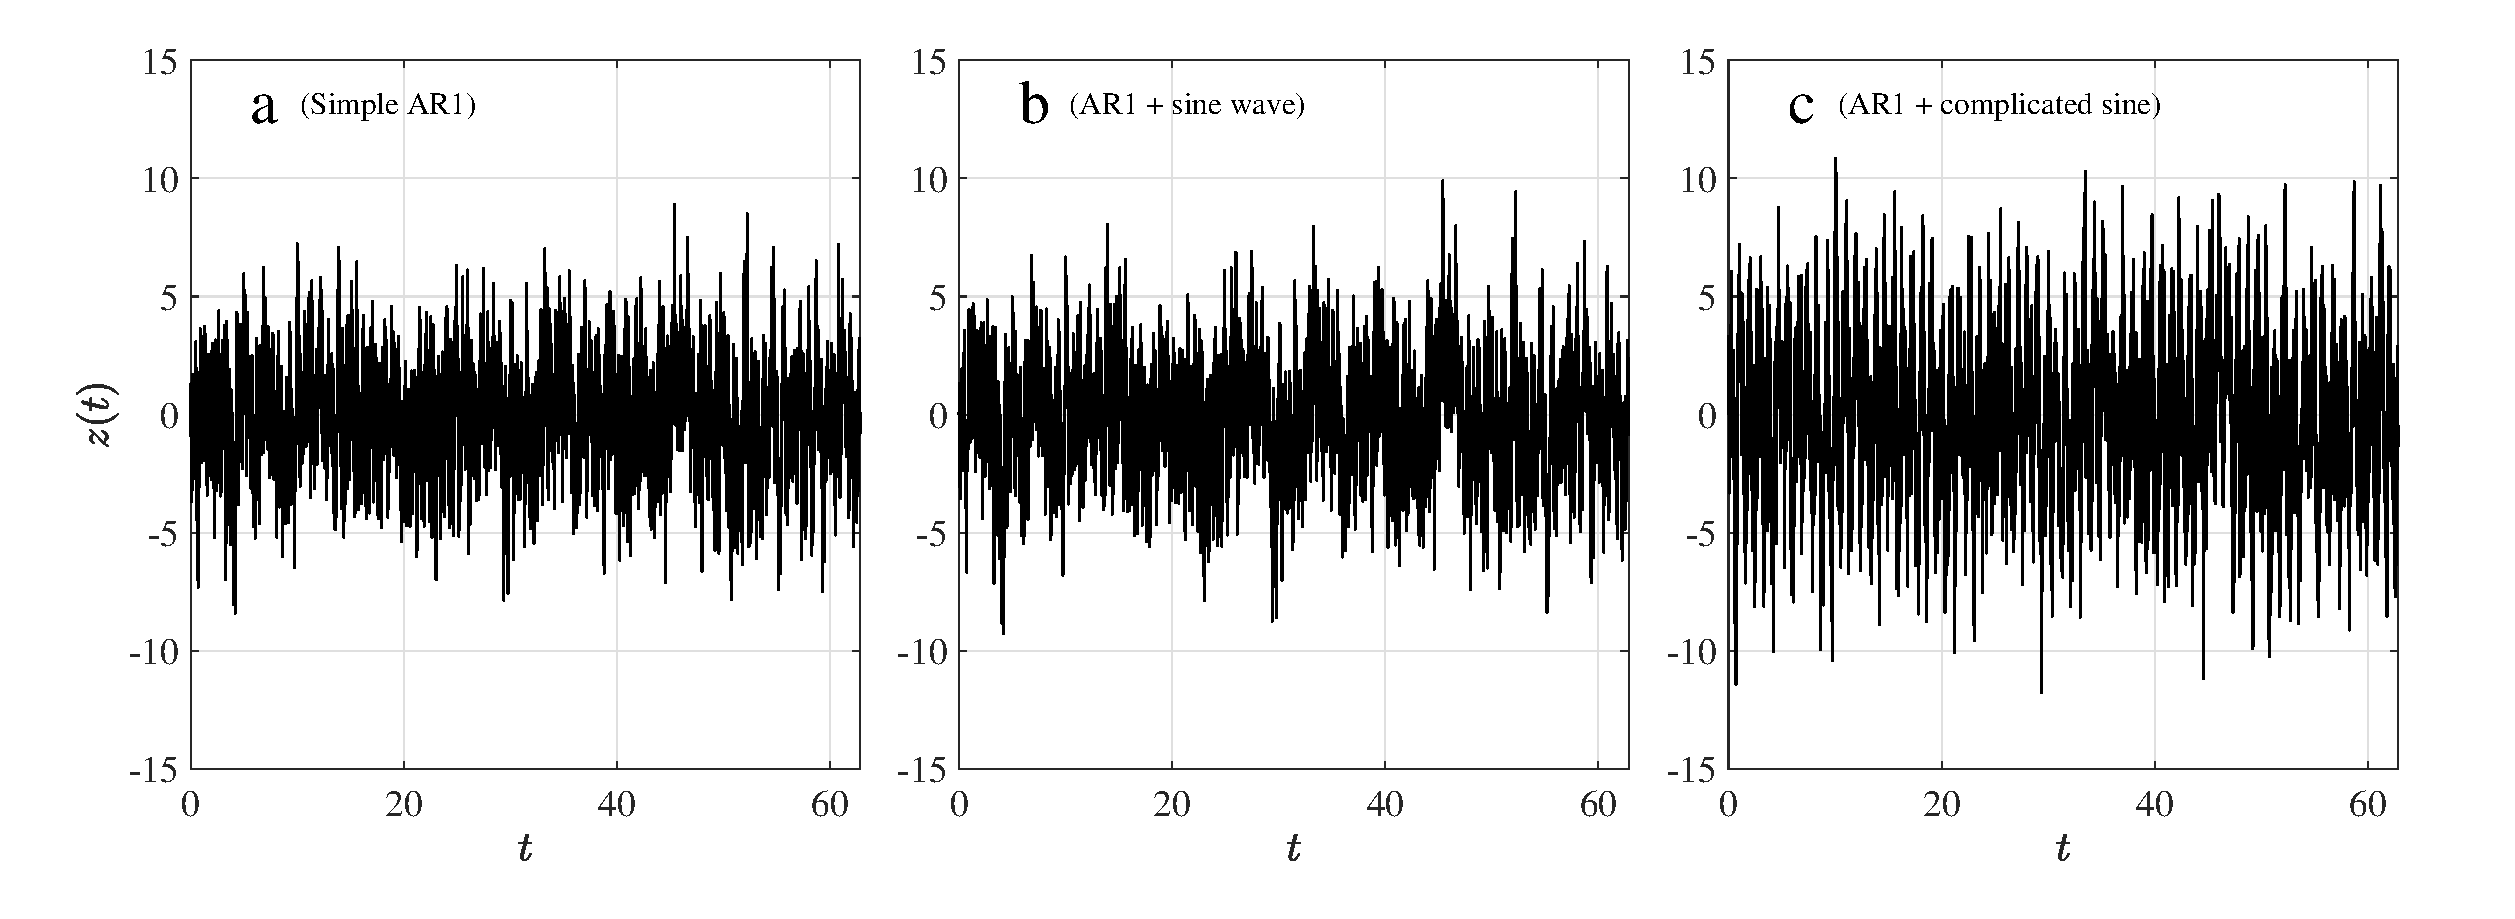
\includegraphics[width=0.9\linewidth]{threeSineWaves}
	\caption{\label{fig:1D:periodicity:threeSineWaves}
		\Red{An AR(1) process of length $10^4$ with parameter $\mu=0.9$ with a periodic function superimposed. Panel {\bf a}: no function. Panel {\bf b}: a simple sine wave $\sin(t)$. Panel {\bf c}: a more complicated function $2\sin(50t)+3\sin(7t)$.}
	}
\end{figure}

{\Red{
In this experiment we take $100$ time series from AR(1) processes
\begin{equation}
	Z_k = \mu Z_{k-1} + \eta_k
\end{equation}
with parameter $\mu$ in the range $[0,1]$. The variance of the Gaussian white noise process $\eta_k$ is $1$. We use time series of length $10^4$ with the artificial time variable $t\in[0, 20\pi]$. From each of these time series $Z(t)$ we create three time series which we use in our analysis:
\begin{enumerate}
	\item The original time series $z(t) = Z(t)$.
	\item The original time series plus a simple sine wave $z(t) = Z(t) + \sin(t)$.
	\item The original time series plus a more complicated function $z(t) = Z(t) + 2\sin(50t)+3\sin(7t)$.
\end{enumerate}
Since the time variable is in the range $[0,20\pi]$, ten periods of the function $\sin(t)$ occur within the time series in each case, whilst $500$ and $70$ periods of the functions $2\sin(50t)$ and $3\sin(7t)$ occur respectively. Each of these is illustrated in figure~\ref{fig:1D:periodicity:threeSineWaves}, which uses $\mu=0.9$ to produce the original AR(1) process. 
}}

\begin{figure}
	% plotted using the Matlab script 'AR1plusSineWavePlot.m'
	\centering
	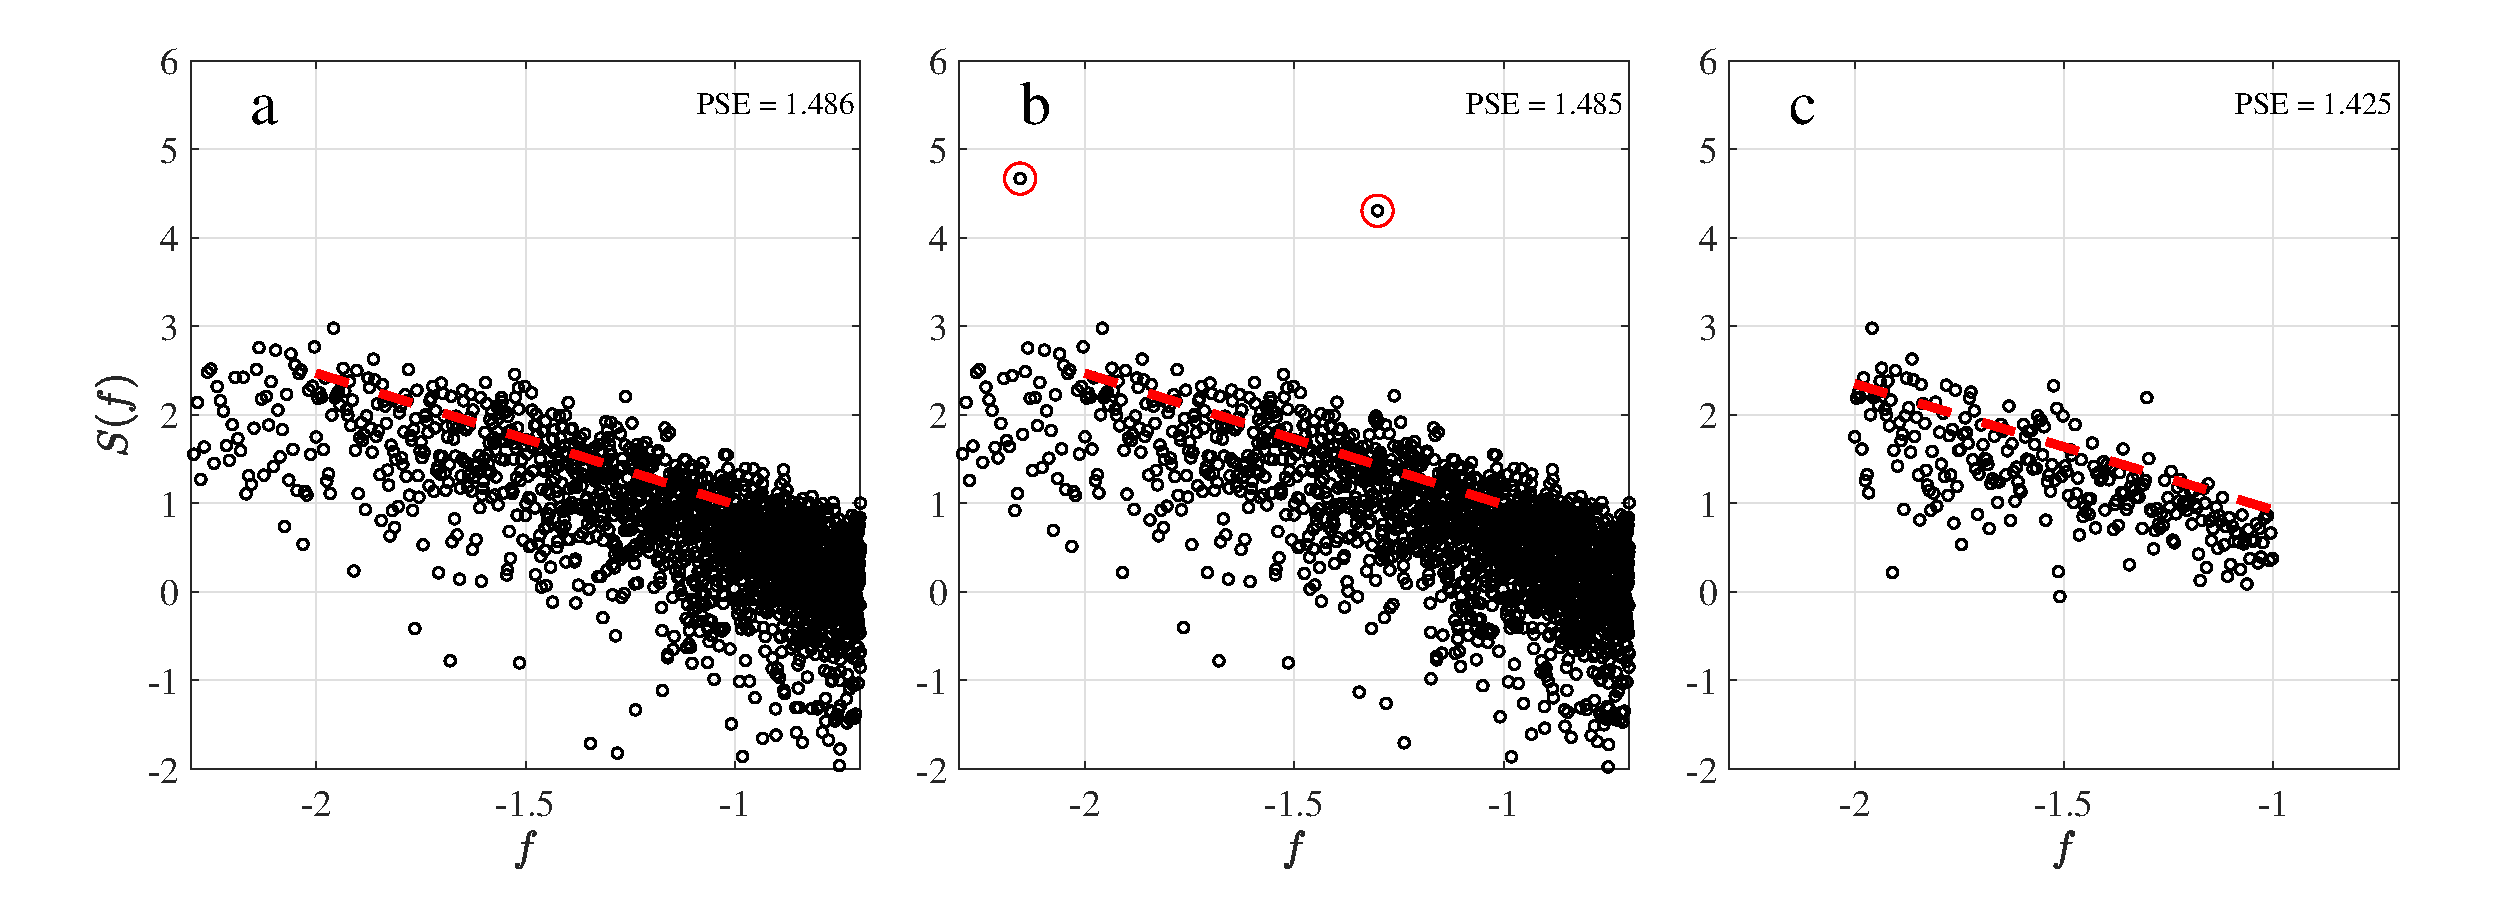
\includegraphics[width=0.9\linewidth]{threePeriodograms}
	\caption{\label{fig:1D:periodicity:threePeriodograms}
		\Red{Panel {\bf a}: periodogram of an AR(1) process.  Panel {\bf b}: periodogram of the same AR(1) process with an added periodic function $g(t) = 2\sin(50t)+3\sin(7t)$. Panel {\bf c}: same as {\bf b} but logarithmic binning has been used. In each case the value of the PS exponent is printed in the top right corner and the line of best fit in the frequency range $\m2\leq\log f\leq\m1$ is plotted in red. The PS exponent for the simple AR(1) process, when using logarithmic binning, is also $1.425$. The power spectrum `spikes' due to the two periodic components are circled in red (panel {\bf b}).  }
	}
\end{figure}

{\Red{
In figure~\ref{fig:1D:periodicity:threePeriodograms} we demonstrate the calculation of the PS exponent for the AR(1) process with $\mu=0.9$. In panels {\bf a} and {\bf b} we compare the periodograms of (respectively) the simple AR(1) process $z(t)=Z(t)$ and the AR(1) with added periodic function $z(t) = Z(t) + 2\sin(50t)+3\sin(7t)$. The power spectral `spikes' due to the two periodic components are circled in red in panel {\bf b}. We note that one spike lies outside of the frequency range used for the estimation of the PS exponent and so will not affect the calculation. The stripped-down periodgram shown in panel {\bf c} of the figure demonstrates the effect of using logarithmic binning to gain a more unbiased estimate of the PS exponent, which is how the exponent is obtained throughout this thesis when using the PS indicator. Once the logarithmic binning is applied the presence of the spikes in the periodogram is even less noticeable, and we find that the value of the PS exponent obtained in this way is the same (to $4$ significant figures) as for the simple AR(1) process without the periodic component. We therefore do not expect that the addition of the periodic series to affect the performance of the PS indicator.

The lag-1 autocorrelation (ACF1), the DFA exponent $\alpha$ and the PS exponent $\beta$ are then calculated for each of these time series and the results are shown in figure~\ref{fig:1D:periodicity:sineWaveAR1}. We note that the ACF1 and DFA are significantly affected by the addition of even a single sine wave with relatively small amplitude (relative to the noise in the AR(1) process, compare figures~\ref{fig:1D:periodicity:threeSineWaves}a and b). As with the introduction of the parabolic trend, the ACF1 is simply scaled up in a consistent way by the introduction of the periodic function, whereas the DFA exponent is affected differently for different values of the parameter $\mu$. The PS exponent, however, is not noticeably affected at all by the introduced periodicity. 
}}

\begin{figure}
	% plotted using the Matlab script 'sineWaveAR1.m'
	\centering
	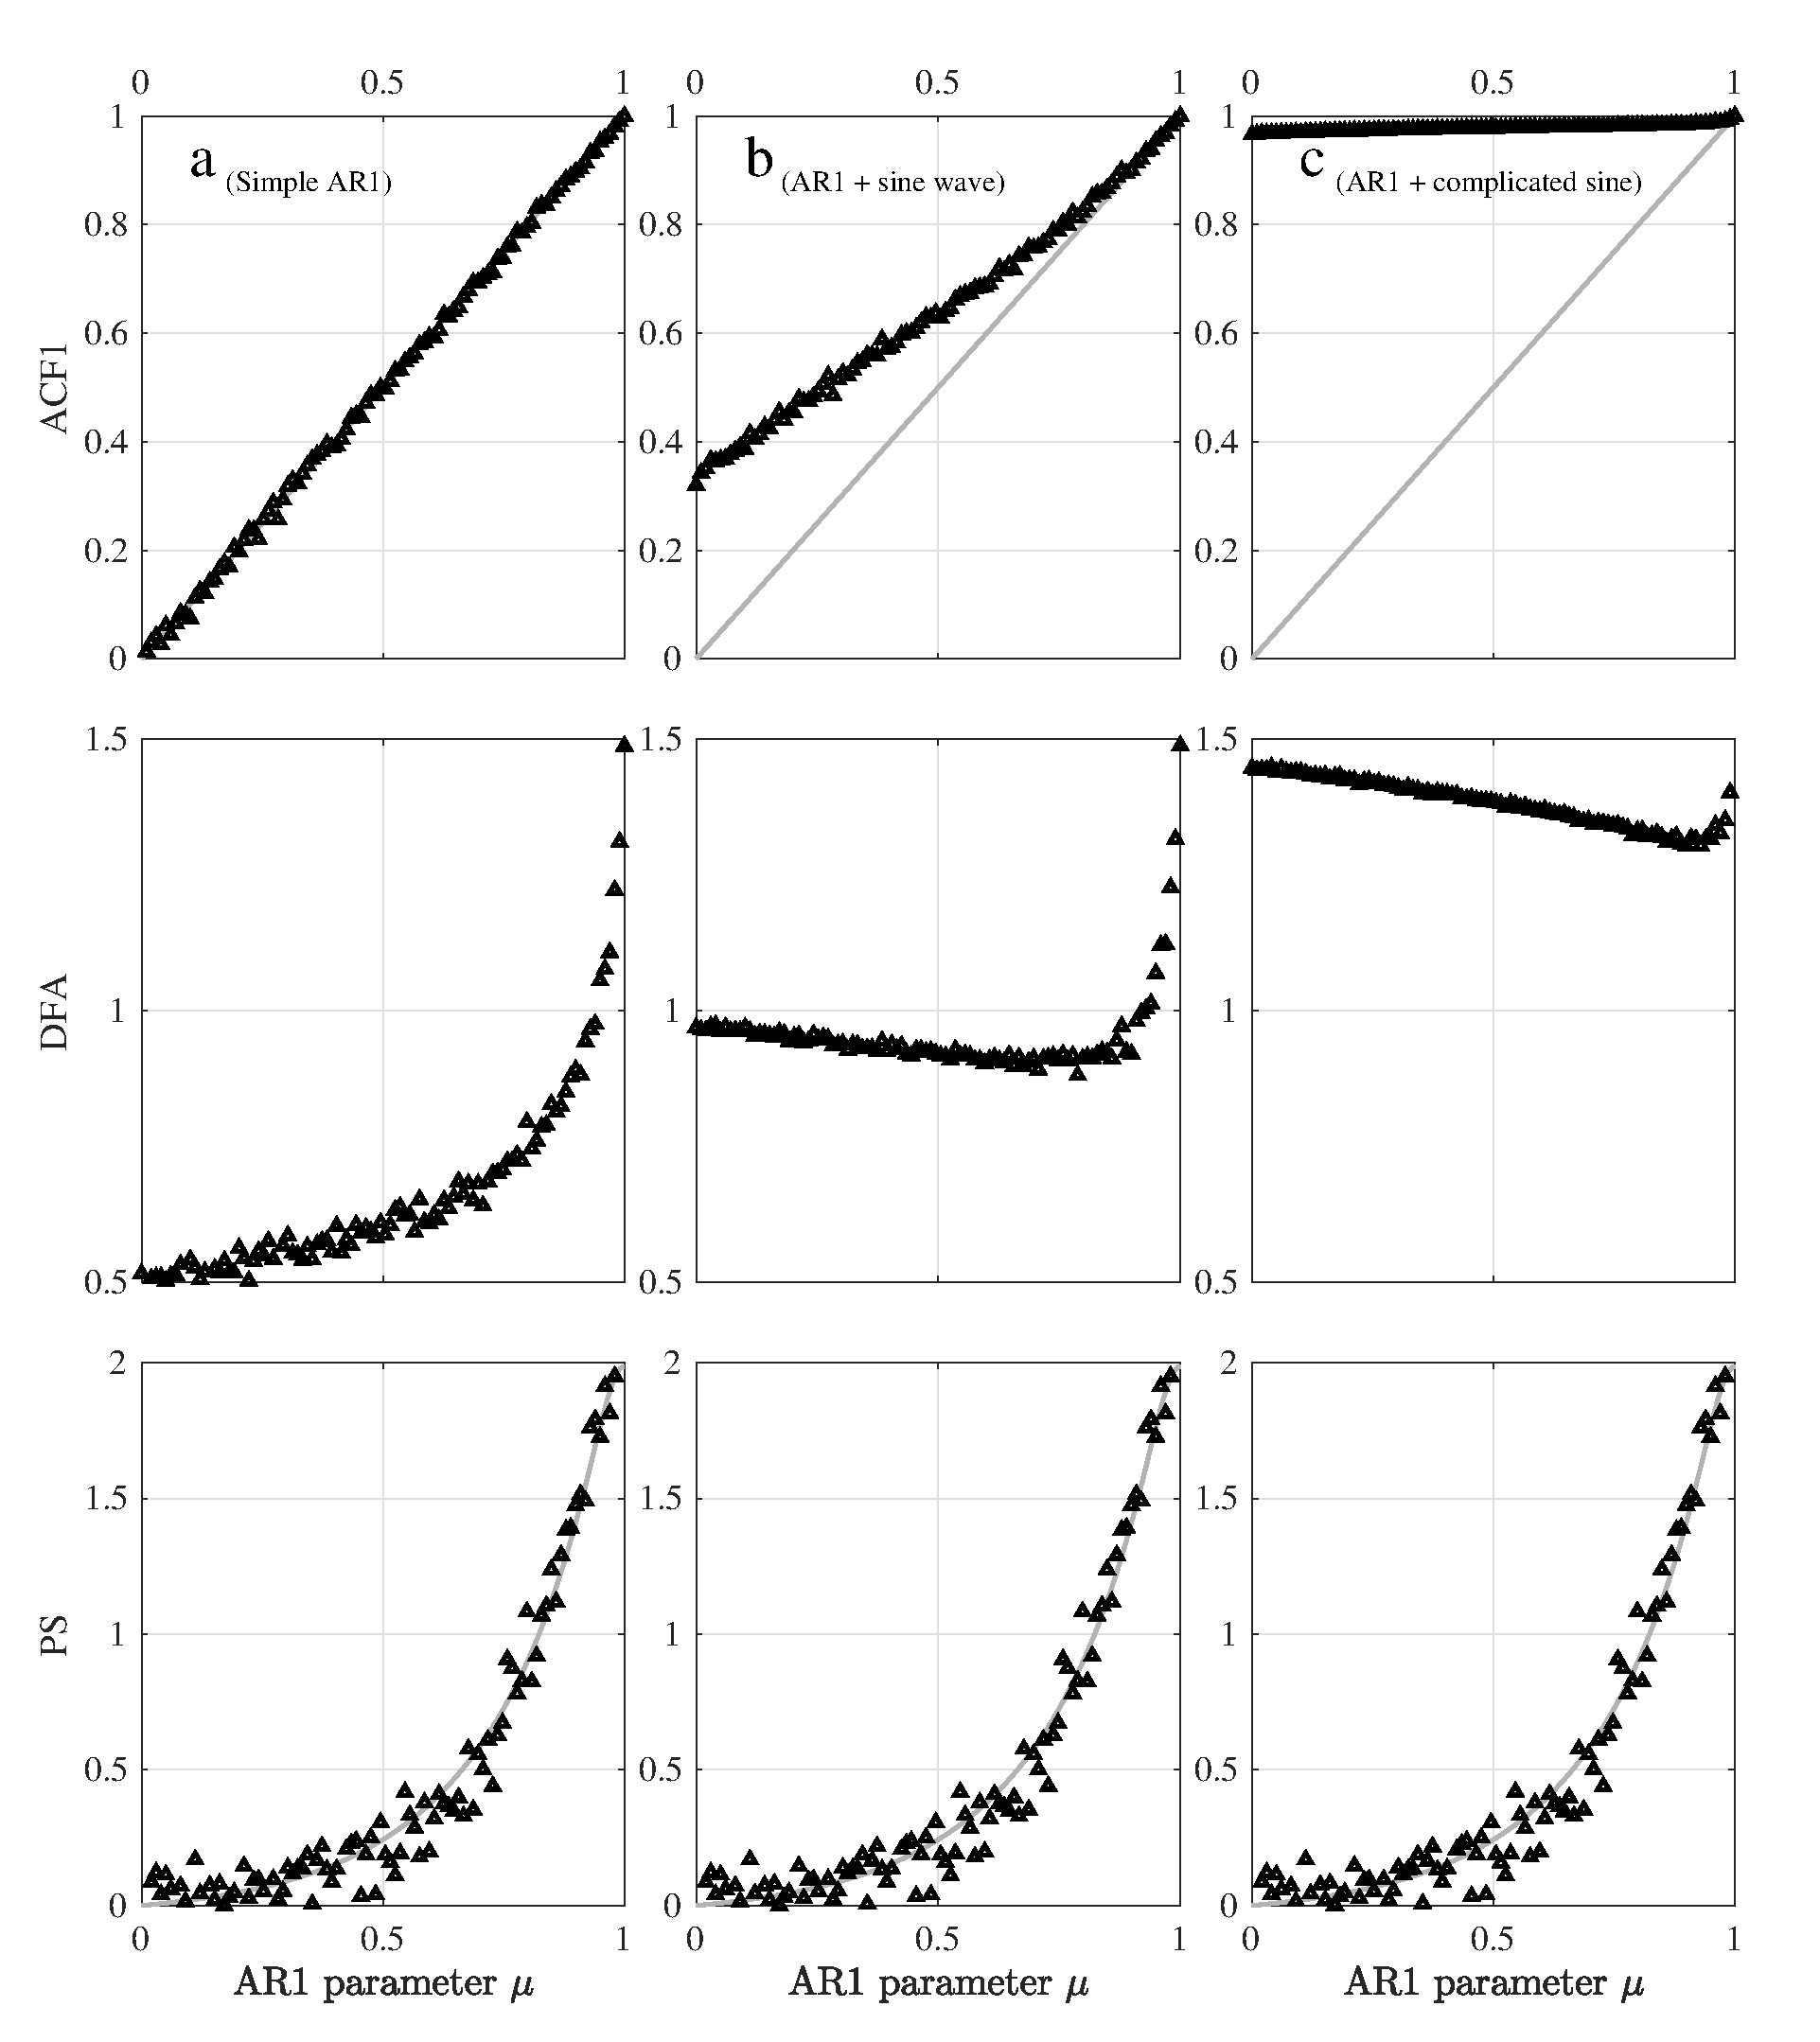
\includegraphics[width=0.9\linewidth]{sineWaveAR1}
	\caption{\label{fig:1D:periodicity:sineWaveAR1}
		\Red{The ACF1 (top row), DFA exponent (middle row) and PS exponent (bottom row) are calculated for $100$ AR(1) time series of length $10^4$ with $\mu\in[0,1]$. The AR(1) time series is super imposed with either no other function (column {\bf a}), a simple sine wave (column {\bf b}), or a more complicated periodic function (column {\bf c}). We note that the PS exponent is practically the same in all three cases. In the case of the ACF1 and PS, the expected value function is plotted in grey.}
	}
\end{figure}

\section{Numerical integration of stochastic ODEs}
\label{sec:1D:numerical_integration}

{\Red 
	
	Throughout this thesis, particularly in this chapter and the next (chapter~\ref{chap:2D}), we obtain a time series by integrating a system of stochastic ODEs (SDEs) and then apply the EWS techniques to this time series, which typically exhibits a tipping point. Such time series, the results of numerical integration of SDEs, have already been presented in chapter~\ref{chap:intro} (see figures~\ref{fig:intro:transitions20_basic} \& \ref{fig:intro:bifurcations20_basic}) without proper explanation of how the integration was performed. 
	
	In initial experiments a simple Euler-Maruyama method, a generalisation of the Euler method to SDEs, was used to integrate one-dimensional systems of the form
		\begin{equation}
		\label{eqn:1D:numerical_integration:standardform}
			\frac{d}{dt}X = f(X,t) + \sigma\eta_t\,,
		\end{equation}
	where $\eta$ is a Gaussian white noise process. Or, using It\^{o} calculus notation,
		\begin{equation}
		\label{eqn:1D:numerical_integration:Ito_form}
			dX = f(X,t)dt + \sigma dW_t\,,
		\end{equation}
	where $W_t$ is a Brownian motion process. For systems of dimension $p>1$, $\eta$ is given as a $p\times 1$ vector and $\sigma$ is a $p\times p$ matrix so that, for example, for the two-dimensional systems of equations
		\begin{equation}
			\begin{array}{rcl}
			\dot{x} &=& y + \sigma_1 \eta^{(x)},\\
			\dot{y} &=& \alpha -  x^2 + \sigma_2\eta^{(y)},
			\end{array}
		\label{eqn:1D:numerical:homoclinicSystem}
		\end{equation}
	where $\eta^{(x)}$ and $\eta^{(y)}$ are two independent Gaussian white noise processes, we have
		\begin{equation}
			f:\begin{pmatrix}
			x\\
			y
			\end{pmatrix}\mapsto \begin{pmatrix}
			y\\
			\alpha - x^2
			\end{pmatrix}\,,
		\end{equation}
	and
		\begin{equation}
			\eta = \begin{pmatrix}
			\eta^{(x)}\\
			\eta^{(x)}
			\end{pmatrix} ~~~\text{and}~~~ \sigma = \begin{pmatrix}
			\sigma_1 & 0\\
			0 & \sigma_2
			\end{pmatrix}\,.
		\end{equation}
	The solution $X(t)$ is approximated by the series $Y_n|_{n=0}^N$ (the Euler–Maruyama approximation), calculated according to
		\begin{equation}
		\label{eqn:1D:numerical_integration:EM_method}
			Y_{n+1} = Y_n + \Delta t f(Y_n,t_n) + \sqrt{\Delta t}\sigma\eta_n\,.
		\end{equation}
	Here the $\eta_n$ are independent identically Gaussian distributed random variables. The $t_n$ form a series with $t_n - t_{n-1} = \Delta t$ and $[t_0, t_N]$ are the lower and upper bounds of integration. The approximation $Y_n$ converges to the true solution $X(t)$ as $\Delta t \rightarrow 0$. 
	
	In several initial experiments in chapter~\ref{chap:2D}, where two-dimensional dynamical systems are presented, the integration of the system of two SDEs was obtained using Matlab's \texttt{ode45} solver \citep{matlab_ode45} which is based on the Dormand-Prince explicit Runge-Kutta (4,5) method \citep{dormand1980family}. This solver is designed for ODEs and does not explicitly handle stochasticity; when including the white noise term $\sigma\eta$ in the solver input, the scaling term $\sqrt{\Delta t}$ was therefore included, as in equation~\ref{eqn:1D:numerical_integration:EM_method}, where $\Delta t$ is specified in the solver input. 
	
	However, Matlab's \texttt{ode45} solver uses an adaptive time step, which may be changed to improve efficiency even if the size of $\Delta t$ is specified by the user. This may then affect the integration of the SDEs since the scaling of the standard deviation of the noise will not be consistent. The Euler-Maruyama method (equation~\ref{eqn:1D:numerical_integration:EM_method}) was therefore used as an alternative, making the method consistent across the thesis, whether dealing with one-dimensional systems given as a single SDE or ODE, or higher dimensional dynamical systems involving systems of two or more SDEs. This is equivalent to the Milstein method for constant $\sigma$ \citep{mackevicius2013introduction}, which is the case in all the two-dimensional systems presented chapter~\ref{chap:2D}. In this chapter (\ref{chap:1D}) and chapter~\ref{chap:cyclones}, however, some models are presented in which the noise scaling factor $\sigma$ is itself a function of time, $\sigma(t)$. The Milstein method, which has superior convergence to the solution \citep{kloeden1999_SDEs}, is therefore used in these cases, where the approximation $Y_n$ is not obtained by equation~\ref{eqn:1D:numerical_integration:EM_method}, but according to 
		\begin{equation}
		\label{eqn:1D:numerical_integration:Milstein}
			Y_{n+1} = Y_n + \Delta t f(Y_n,t_n) + \sqrt{\Delta t}\sigma(t_n)\eta_n + \frac{1}{2}\sigma(t_n)\sigma'(t_n)\Delta t\left((\sigma(t_n) \eta_n)^2-1\right)\,.
		\end{equation}
	where $\sigma'$ is the derivative of $\sigma$ with respect to $X$ and is estimated using 
		\begin{equation}
		\label{eqn:1D:numerical:sigmadash}
			\frac{d}{dx}\sigma = \left(\frac{dt}{dx}\right)^{\m1}\cdot\frac{\partial \sigma}{\partial t} \approx \left(\frac{\Delta t f(Y_n,t_n) + \sqrt{\Delta t}\sigma(t_n)\eta_n}{\Delta t}\right)^{\m1} \cdot \frac{\sigma(t_{n+1})- \sigma(t_n)}{\Delta t}\,,
		\end{equation}
	or 
		\begin{equation}
			\sigma'(t_n) \approx \frac{\sigma(t_{n+1})- \sigma(t_n)}{\Delta t f(Y_n,t_n) + \sqrt{\Delta t}\sigma(t_n)\eta_n}\,,
		\end{equation}
	where we have used the Euler-Maruyama method in the estimation of $dx/dt$. We note that the numerator $\sigma(t_{n+1})- \sigma(t_n)$ ensures that the whole last term in equation~\ref{eqn:1D:numerical_integration:Milstein} is indeed zero where $\sigma$ is constant, thus ensuring that this is equivalent to the Euler-Maruyama method in equation~\ref{eqn:1D:numerical_integration:EM_method}. For systems of dimension $p>1$, equation~\ref{eqn:1D:numerical:sigmadash} becomes problematic since the `numerator' $\dot{\Sigma} := \sigma(t_{n+1})- \sigma(t_n)$ is a $p\times p$ matrix and the `denominator' $\dot{X} := \Delta t f(Y_n,t_n) + \sqrt{\Delta t}\sigma(t_n)\eta_n$ is a $p\times 1$ vector. In this case we perform the element-wise reciprocal operation on $\dot{X}$ and then take the matrix product	
	\begin{equation}
	\sigma'(t_n) = \begin{pmatrix}
	(\dot{x}_1)^{\m1} &  & 0\\
	  & \ddots & \\
	0  &  & (\dot{x}_p)^{\m1}
	\end{pmatrix} \dot{\Sigma}~~~~\text{where}~~~\dot{X} = \begin{pmatrix}
	\dot{x}_1\\
	\vdots\\
	\dot{x}_p\,.
	\end{pmatrix}\,.
	\end{equation}
	Concerning the term $(\sigma(t_n) \eta_n)^2$ in equation~\ref{eqn:1D:numerical_integration:Milstein}, the vector $\sigma(t_n) \eta_n$ is first calculated and the square operation is performed element wise before the vector of ones is subtracted. 
	
	In this chapter many one-dimensional systems are defined by an SDE in the form
		\begin{equation}
		\label{eqn:1D:numerical_integration:potentialform}
			\dot{z}(t) = -\frac{\partial}{\partial z}U(z,t) + \sigma(t)\eta_t\,,
		\end{equation}
	where $U$ is the generalised potential function of $z$ which may also change over time. This formulation is convenient as it allows us to visualise the stable points (troughs or `wells') and unstable points (peaks) of the state space. In these cases the system is not of the form in equation~\ref{eqn:1D:numerical_integration:standardform} since we have the negative derivative of $U$, rather than the function $f$. The function $f$ is either obtained analytically by taking the derivative of $U$ with respect to $z$, in cases where $U$ is a function of $z$ only; or, if this is complicated due to a time dependence in $U$, the function $f$ is estimated at each stage in the Milstein algorithm using 
		\begin{equation}
		\label{eqn:1D:numerical_integration:function_estimate}
			f(Y_n, t_n) = 	-\frac{U(Y_n+\varepsilon, t_n)-U(Y_n-\varepsilon, t_n)}{2\varepsilon}\,,
		\end{equation}
	where the small step $\varepsilon$ is chosen as $\varepsilon=\min(\Delta t, 10^{-5})$ to reduce error over simply using $\varepsilon=\Delta t$ in the case that $\Delta t$ is large, although we typically use small values of $\Delta t$ anyway. 
	
	The Milstein method, given by equation~\ref{eqn:1D:numerical_integration:Milstein} (or the equivalent Euler-Maruyama method where $\sigma$ is constant), is used consistently throughout this thesis for all numerical integration of SDEs, including where system equations are given in the generalised potential form, in which case the function $f$ is estimated using equation \ref{eqn:1D:numerical_integration:function_estimate} if it cannot be obtained analytically.
	
	In cases where Matlab's \texttt{ode45} solver had already been used at the stage of experimentation to integrate two-dimensional systems of SDEs presented in chapter~\ref{chap:2D}, the same systems were integrated again using the Milstein method, in which the scaling of the time step is handled properly, although the method itself is much simpler than the Runge-Kutta (4,5) method with inferior convergence for ODEs \citep{mackevicius2013introduction}. In all cases where both methods were used there was no visible difference between the two, nor any difference in the calculated early warning signals, suggesting that the error due to the adaptive time step problem was, in fact, negligible. Similarly, where the simpler Euler-Maruyama method had been used at the stage of experimentation to integrate one-dimensional SDEs with non-constant $\sigma$, these same systems were integrated again using the Milstein method.
	
	
}



\section{Early Warning Signals in dynamical systems}
\label{sec:1D:indicatorComparison}

{\Red In this section we apply the DFA, PS and ACF1 indicators to several  examples of time series containing tipping points. The first system we study is constructed from segments of generated noise, artificially designed to have a gradually increasing power spectrum scaling exponent, which is used by \cite{livina2012} as a test of the DFA indicator method. We use the same system here to offer a direct comparison between that and the novel PS indicator \citep{prettyman2018}. We then apply the PS indicator and the ACF1 indicator to the three examples presented in chapter~\ref{chap:intro} (see section~\ref{subsec:intro:tippingpoints:defining_a_tipping_point}) which represent the three types of tipping point as outlined by \cite{livina2011}, and also a variety of different bifurcational tipping points occurring in one-dimensional systems. Some of these we go on to study in more detail and also apply the DFA indicator for comparison. In no case do we suppose that there is some critical value of the indicator which gives us special information about a tipping point. Rather, it is the behaviour of the indicator over time which we expect to precede a tipping point. In the cases of the ACF1, DFA and PS indicators used in this chapter, it is an \emph{increasing trend} that we look for, whatever the actual values of the indicators themselves.
		
In this section, and at other points throughout this thesis, a dynamical system is defined analytically as a stochastic ODE and then integrated numerically in Matlab to produce a time series of data. The Milstein method of numerical integration, as defined in the previous section, is used consistently throughout (see section~\ref{sec:1D:numerical_integration}).
}

{\Red{The results of the application to the supercritical pitchfork bifurcation (section~\ref{subsec:1D:indicatorComparison:PitchforkModel}) have previously been presented in \cite{prettyman2018}.}}

\subsection{Choice of model parameters}
\label{subsec:1D:indicatorComparison:choice_of_parameters}
{\Red{
The work presented in this section and, later, in chapter~\ref{chap:2D} makes heavy use of `toy' dynamical system models in our investigation of EWS techniques. Such toy models, particularly those exhibiting a bifurcation, have some critical parameter $\mu$ which is varied within a range of values and the bifurcation or other tipping point occurs in the system when $\mu$ is equal to some critical value $\mu_\text{crit}$. In this case it is necessary to make a choice of the values of this parameter to be used, as well as how fast to vary this parameter if the model involves a changing value. We consider several factors affecting the choice of the parameters:
\begin{enumerate}
	\item That the different values of the parameter demonstrate a significant qualitative change in the system, indicative of a tipping point. It is often the case that if values of the parameter $\mu$ are considered over the interval $[\mu_\text{crit}-\rho, \mu_\text{crit}+\rho]$, where $\rho$ is very small, the real behaviour of the system may not apparently change very much, despite a bifurcation having occurred. This is quite clearly the case for the supercritical pitchfork bifurcation which changes smoothly from the pre-tipping state space to the post-tipping state space, although it may not be so important with fast-diverging `blow up' systems (e.g. subcritical pitchfork bifurcation).
	\item That the rate of change of the parameter is slow relative to the recovery time of the system. This is an essential consideration since the EWS methods studied here are based on detecting critical slowing down which is a measure of decreasing recovery times. 
	\item That the rate of change of the parameter is slow relative to the numerical time step, since no EWS will be visible if a very large change from the pre-tipping state space to the post-tipping state space occurs in a single step. In any case, such a fast-changing parameter would also affect the previous point since the system would not have time to recover. 
\end{enumerate} 
In general, the choice of model parameters is considered with the aim of facilitating a useful comparison between the novel PS indicator and the ACF1 and DFA indicators, often in similar dynamical systems to those in which these existing methods have already been tested (see \cite{livina2007}), which is the purpose of this study. The problem of detecting critical slowing down, and therefore detecting tipping points, in systems with a relatively fast rate of change of critical parameters is a potentially interesting topic for future work, and may be related to the fast-growing field of \emph{rate-induced tipping points} (see \cite{ritchie2016rate}), but it is not within the scope of the work presented here. 

In addition to the choice of tipping-critical model parameters, it is also necessary to select appropriate values for other system parameters. In particular most of the toy models used in this section and in the following chapter are stochastic systems in which the system equations incorporate a white noise process the size of which may greatly affect the behaviour of the system and the performance of the EWS methods. In all cases, the variance of the noise must be large enough that the system is `perturbed' significantly from the stable state, and that there might be some variation within an ensemble of several integrations of the system (in a purely deterministic system there would be no variation between members of the ensemble). Yet, the variance must also be small enough that the noise does not completely mask the deterministic component of the system. In a system defined by the stochastic differential equation
	\begin{equation}
		\dot{z} = f(z,t) +\sigma\eta\,,
	\end{equation}
where $\eta$ is a Gaussian white noise process, if $\sigma$ is very large compared to the value of $f(z,t)$ for $z,t$ in the range of integration, the integrated time series $z(t)$ will be essentially a random walk, and incorporate none of the deterministic dynamics of the function $f$. In cases where we expect to see noise-induced tipping, and we aim to assess the usefulness of the early warning indicators in that context, the variance of the noise is of course chosen that noise-induced tipping may indeed be observed. Where such noise-induced tipping is brought about by a change the stochastic component of the system, where the variance of the noise term is a parameter with some critical value at which tipping occurs, the rate of change of this parameter is chosen, as with deterministic parameters, such that the tipping may be observed in the integrated time series and that the rate of change is not on time scales faster than the deterministic evolution of the system.  
}}
	



\subsection{Early warning signals in an artificial stochastic signal}
\label{sec:1D:ArtificialModel} 

\begin{figure}
	\centering
	
\includegraphics[width = 0.9\textwidth]{fig2_v5}
	\caption{Artificial data with ACF1, DFA and PS indicators. (a) A time series is constructed by concatenating 50 sub-series of length 200 where the scaling exponent $\beta$ within each sub-series is constant and increases over the whole series from 0 (white noise) to 2. (b,c,d) The ACF1, DFA and PS indicator methods are applied with window size 100. As the PS-indicator increases from 0 to 2, the ACF indicator increases from 0 to 1, and the DFA indicator $\alpha$ increases from 0.5 to 1.5. Lines are added to show the linear trends; note that the ACF indicator does not increase linearly as it approaches 1. \label{fig:1D:ArtificialSignal}}
\end{figure}

 \citet{livina2012} compare the performance of the ACF1 and DFA indicators when applied to an artificially constructed time series with increasing PS scaling exponent. The series is created by concatenating many shorter sub-series with specific, incrementally increasing power spectrum scaling exponents $\beta$ from white noise ($\beta=0$) in the first sub-series to red noise ($\beta=2$) in the final series.  
 
 Here, we recreate the experiment in order to compare the ACF1, DFA and PS indicators. We create 50 sub-series each of length 200 points with incrementally increasing PS exponents. To achieve this, for each sub-series we take a white noise signal $X(t)$, apply a fast Fourier transform and then multiply the power spectrum $\hat{X}(f)$ by a factor of $\sqrt{f^{-\beta}}$ where $\beta$ is the desired PS exponent (see also equation \ref{eqn:1D:creatingColouredNoise}). The resulting power spectrum is then transformed back to the time domain using an inverse fast Fourier transform \citep{makse1996}. The values of $\beta$ increase linearly in the range $[0, 2]$, changing from white noise to red noise. The 50 series are then joined to create a series of length $10^4$. We note that this is an example of a time series which experiences a rise in autocorrelation simultaneously with a decrease in variance. 
 
 
 
The ACF1, DFA and PS indicators are applied to the constructed series. Since the series is specifically constructed to have an increasing PS exponent, we expect to see an increasing trend in the PS indicator. We also expect the same behaviour in the DFA indicator because of the relationship between the two exponents (see figure \ref{fig:1D:ExponentRelationships}). We also know that lag-1 ACF increases with increasing PS exponent in long-range correlated noise (figure \ref{fig:1D:ACFrelationships}) and so expect that the ACF1 indicator will also show an increasing trend when applied to our series.

Figure \ref{fig:1D:ArtificialSignal} shows the signal (panel {\bf a}) and the results of applying the three indicators (panels {\bf b}, {\bf c}, {\bf d}) along with the linear best fit. As in our previous experiment which calculated the lag-1 ACF for noise series with different values of $\beta$ (figure \ref{fig:1D:ACFrelationships}), the lag-1 ACF increases linearly with increasing $\beta$ only up to a point, approximately $\beta = 1$, after which the rate of increase slows. The DFA and PS increase linearly, as expected, with increasing $\beta$ and the relationship between the two indicators obeys the same linear law connecting to DFA and PS exponents (equations \ref{eqn:1D:alphabetaExponentRelationships}). The variance in both indicator series is also similar, and so we have evidence for the assertion that it is not necessary to use the PS exponent when the DFA exponent is available \citep{heneghan2000}, but concerning the sliding-window indicator methods, rather than a simple calculation of the exponents.

\begin{landscape}
	\begin{figure}
		\centering
		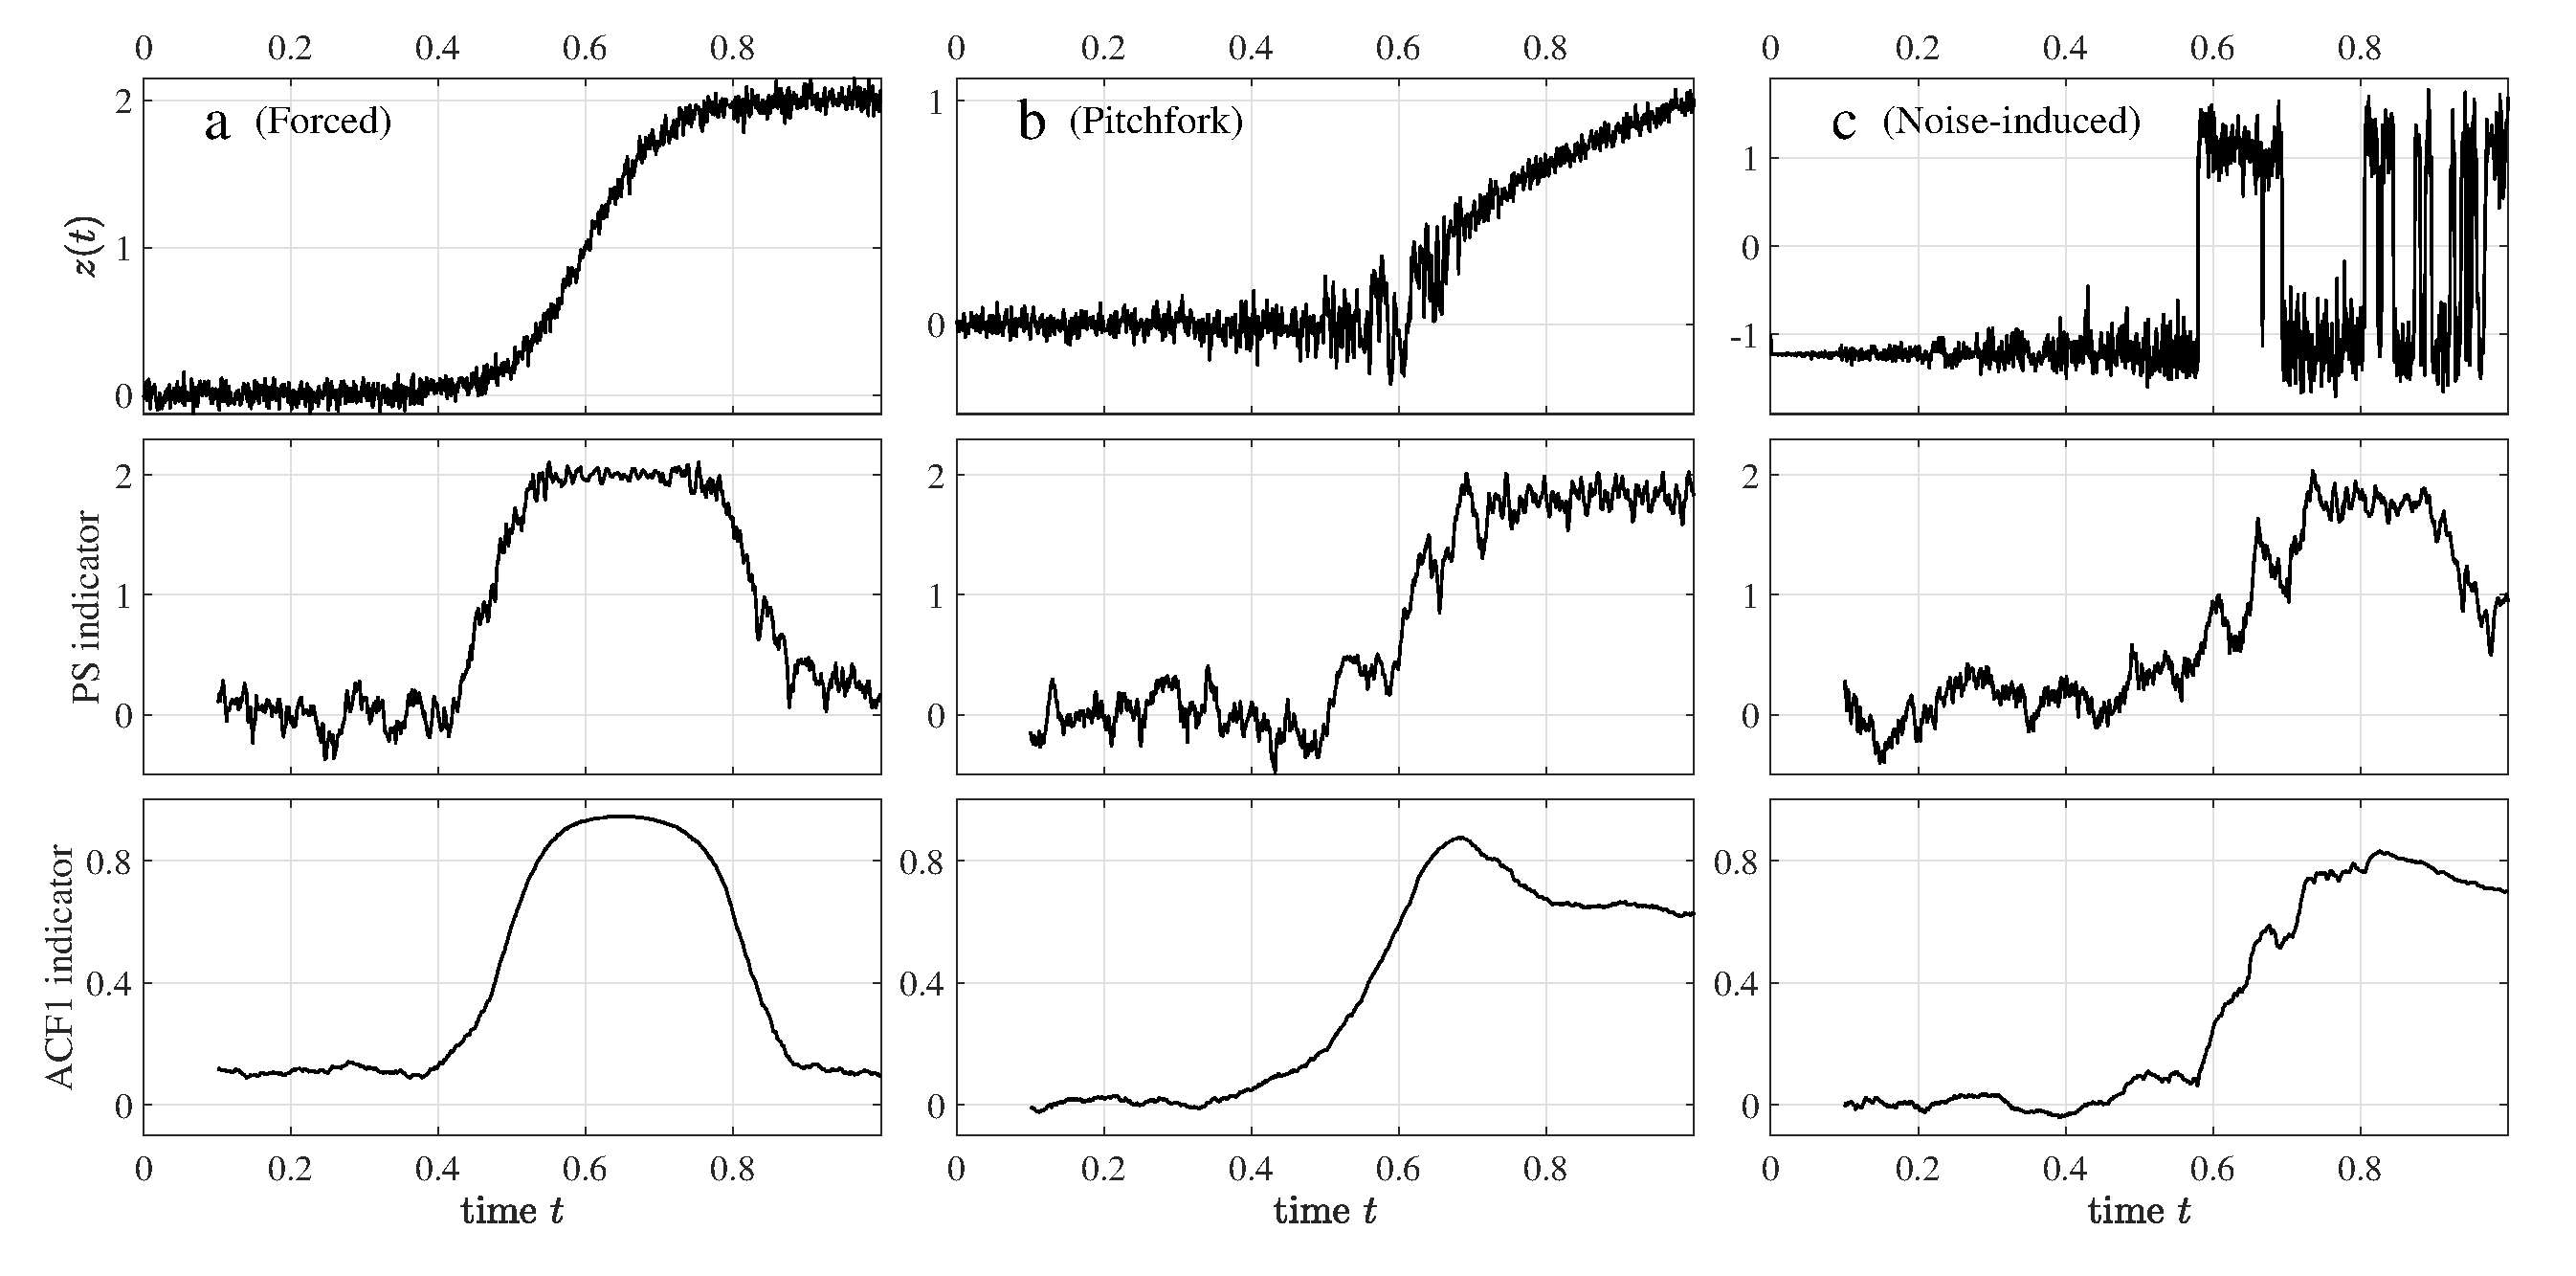
\includegraphics[width=\linewidth,keepaspectratio]{transitions30}
		\caption{\Red{Three systems given by equations~\ref{eqn:1D:DifferentTypesOfTipping:forced} (forced transition), \ref{eqn:1D:DifferentTypesOfTipping:genuine} (pitchfork bifurcation), and \ref{eqn:1D:DifferentTypesOfTipping:noise-induced} (noise-induced tipping point) are integrated between $t=0$ and $t=1$. Each exhibits a tipping point at around $t=0.6$: a forced transition, a pitchfork bifurcation, and a noise-induced transition (panels {\bf a}, {\bf b}, {\bf c} respectively). The PS and ACF1 indicators are calculated using a sliding window of 100 points and plotted beneath the time series for each system. We note the similarity in shape between the two indicator signals, although the PS indicator is more noisy. }
		}
		\label{fig:1D:threesystemswithPSandACF}
	\end{figure}
\end{landscape}

\subsection{Early warning signals for three distinct tipping points}
 \label{subsec:1D:indicatorComparison:TypesOfTipping}

{\Red
 In section~\ref{sec:intro:classification_of_TPs}, chapter~\ref{chap:intro}, we presented three examples of dynamical systems each exhibiting one of the three types of tipping point suggested by \cite{livina2011}: A forced transition, a genuine bifurcation, and a noise-induced transition. 
 
 We give the equations for each of these three examples again here. In each case the system equation is in the `generalised potential' form of equation~\ref{eqn:1D:numerical_integration:potentialform} and integrated numerically using the Milstein method (see section~\ref{sec:1D:numerical_integration}) with time step $\Delta t = 10^{\m 5}$ and a sampling rate of $10^3$ per unit time. Thus each integration generates a time series of $1000$ points since the time range in each case is $t\in [0,1]$.

\subsubsection{Type 1: Forced transition}
As an example of a `forced transition' we use the system described by the equation 
\begin{equation}
\label{eqn:1D:DifferentTypesOfTipping:forced}
\dot{z}(t) = -\frac{\partial }{\partial z}\left(z-\tanh(10t-6)-1\right)^2 + \frac{1}{10}\eta \, ,
\end{equation}
where $\eta$ is a Gaussian white noise process. This system has a quadratic-shape generalised potential which shifts in position over time. For small $t$, that is $t<0.5$, the stable equilibrium, the base of the `well', is at the position $z\approx 0$. This shifts to the position $z\approx 2$ when $t>0.7$. Thus, a sudden shift occurs around $t=0.6$, as we can see in figure~\ref{fig:1D:threesystemswithPSandACF}a. 

We note that both the PS and ACF1 indicators begin to rise about the same time that the shift in the stable point becomes visually obvious, and have reached their maximum values before the system is halfway through the transition. 

\subsubsection{Type 2: Genuine bifurcation}
As an example of a genuine bifurcation we present the familiar pitchfork bifurcation, already used as an example in this chapter, given by the equation:
	\begin{equation}
	\label{eqn:1D:DifferentTypesOfTipping:genuine}
		\dot{z}(t) = -\frac{\partial }{\partial z}\left(z^4+(3-5t)z^2\right) + \frac{1}{10}\eta\,,
	\end{equation}
where $\eta$ is a Gaussian white noise process. In this case the bifurcation occurs at $t=0.6$. We see in figure~\ref{fig:1D:threesystemswithPSandACF}b the apparent increase in ``white'' noise just before $t=0.6$ as the base of the `well' flattens out and allows for longer and longer return times to the equilibrium point $z=0$.

Again we note that the PS and ACF1 indicators show similar behaviour, although the PS indicator is more noisy. In both cases the increasing trend in the indicator begins before the bifurcation occurs at $t=0.6$.


\subsubsection{Type 3: Noise-induced transition}
As an example of a noise-induced transition we take a `double-well' generalised potential with added noise and allow the standard deviation of the noise to increase with time. At some \emph{critical point} the noise is large enough that the system is able to escape from the `well' and switch to the other stable state. The time series in figure~\ref{fig:1D:threesystemswithPSandACF}c is described by the equation:
\begin{equation}
\label{eqn:1D:DifferentTypesOfTipping:noise-induced}
\dot{z}(t) = -\frac{\partial }{\partial z}\left(z^4-3z^2\right) + \frac{3t}{2} \eta\,,
\end{equation}
where $\eta$ is a Gaussian white noise process and the coefficient $\sigma(t) = 3t/2$ modifies the standard deviation of the noise as a function of $t$. At around $t=0.6$ the noise standard deviation is close to $1$ which is about large enough that state-switching becomes likely though not frequent. As $t$ increases further, the frequency of the state-switch increases. 

Once again we note the correlation between the PS and ACF1 indicators. In this example the increasing trend in the indicators does not begin until the noise is already large enough that the system is able to tip into the other stable state. This is due simply to the shape of the generalised potential function in this particular case. For this type of system where a Gaussian white noise process is integrated, an increase in the size of the noise will always cause an increase in the PS exponent, whether it leads to a tipping point or not. This type of tipping is not characterised by the critical slowing down phenomenon, unlike the pitchfork bifurcation of the previous example. We don't therefore expect that the PS indicator will necessarily provide an EWS, although it will, of course, provide information about the nature of the noise in the series. 
 

}


\begin{landscape}
	\begin{figure}
		\centering
		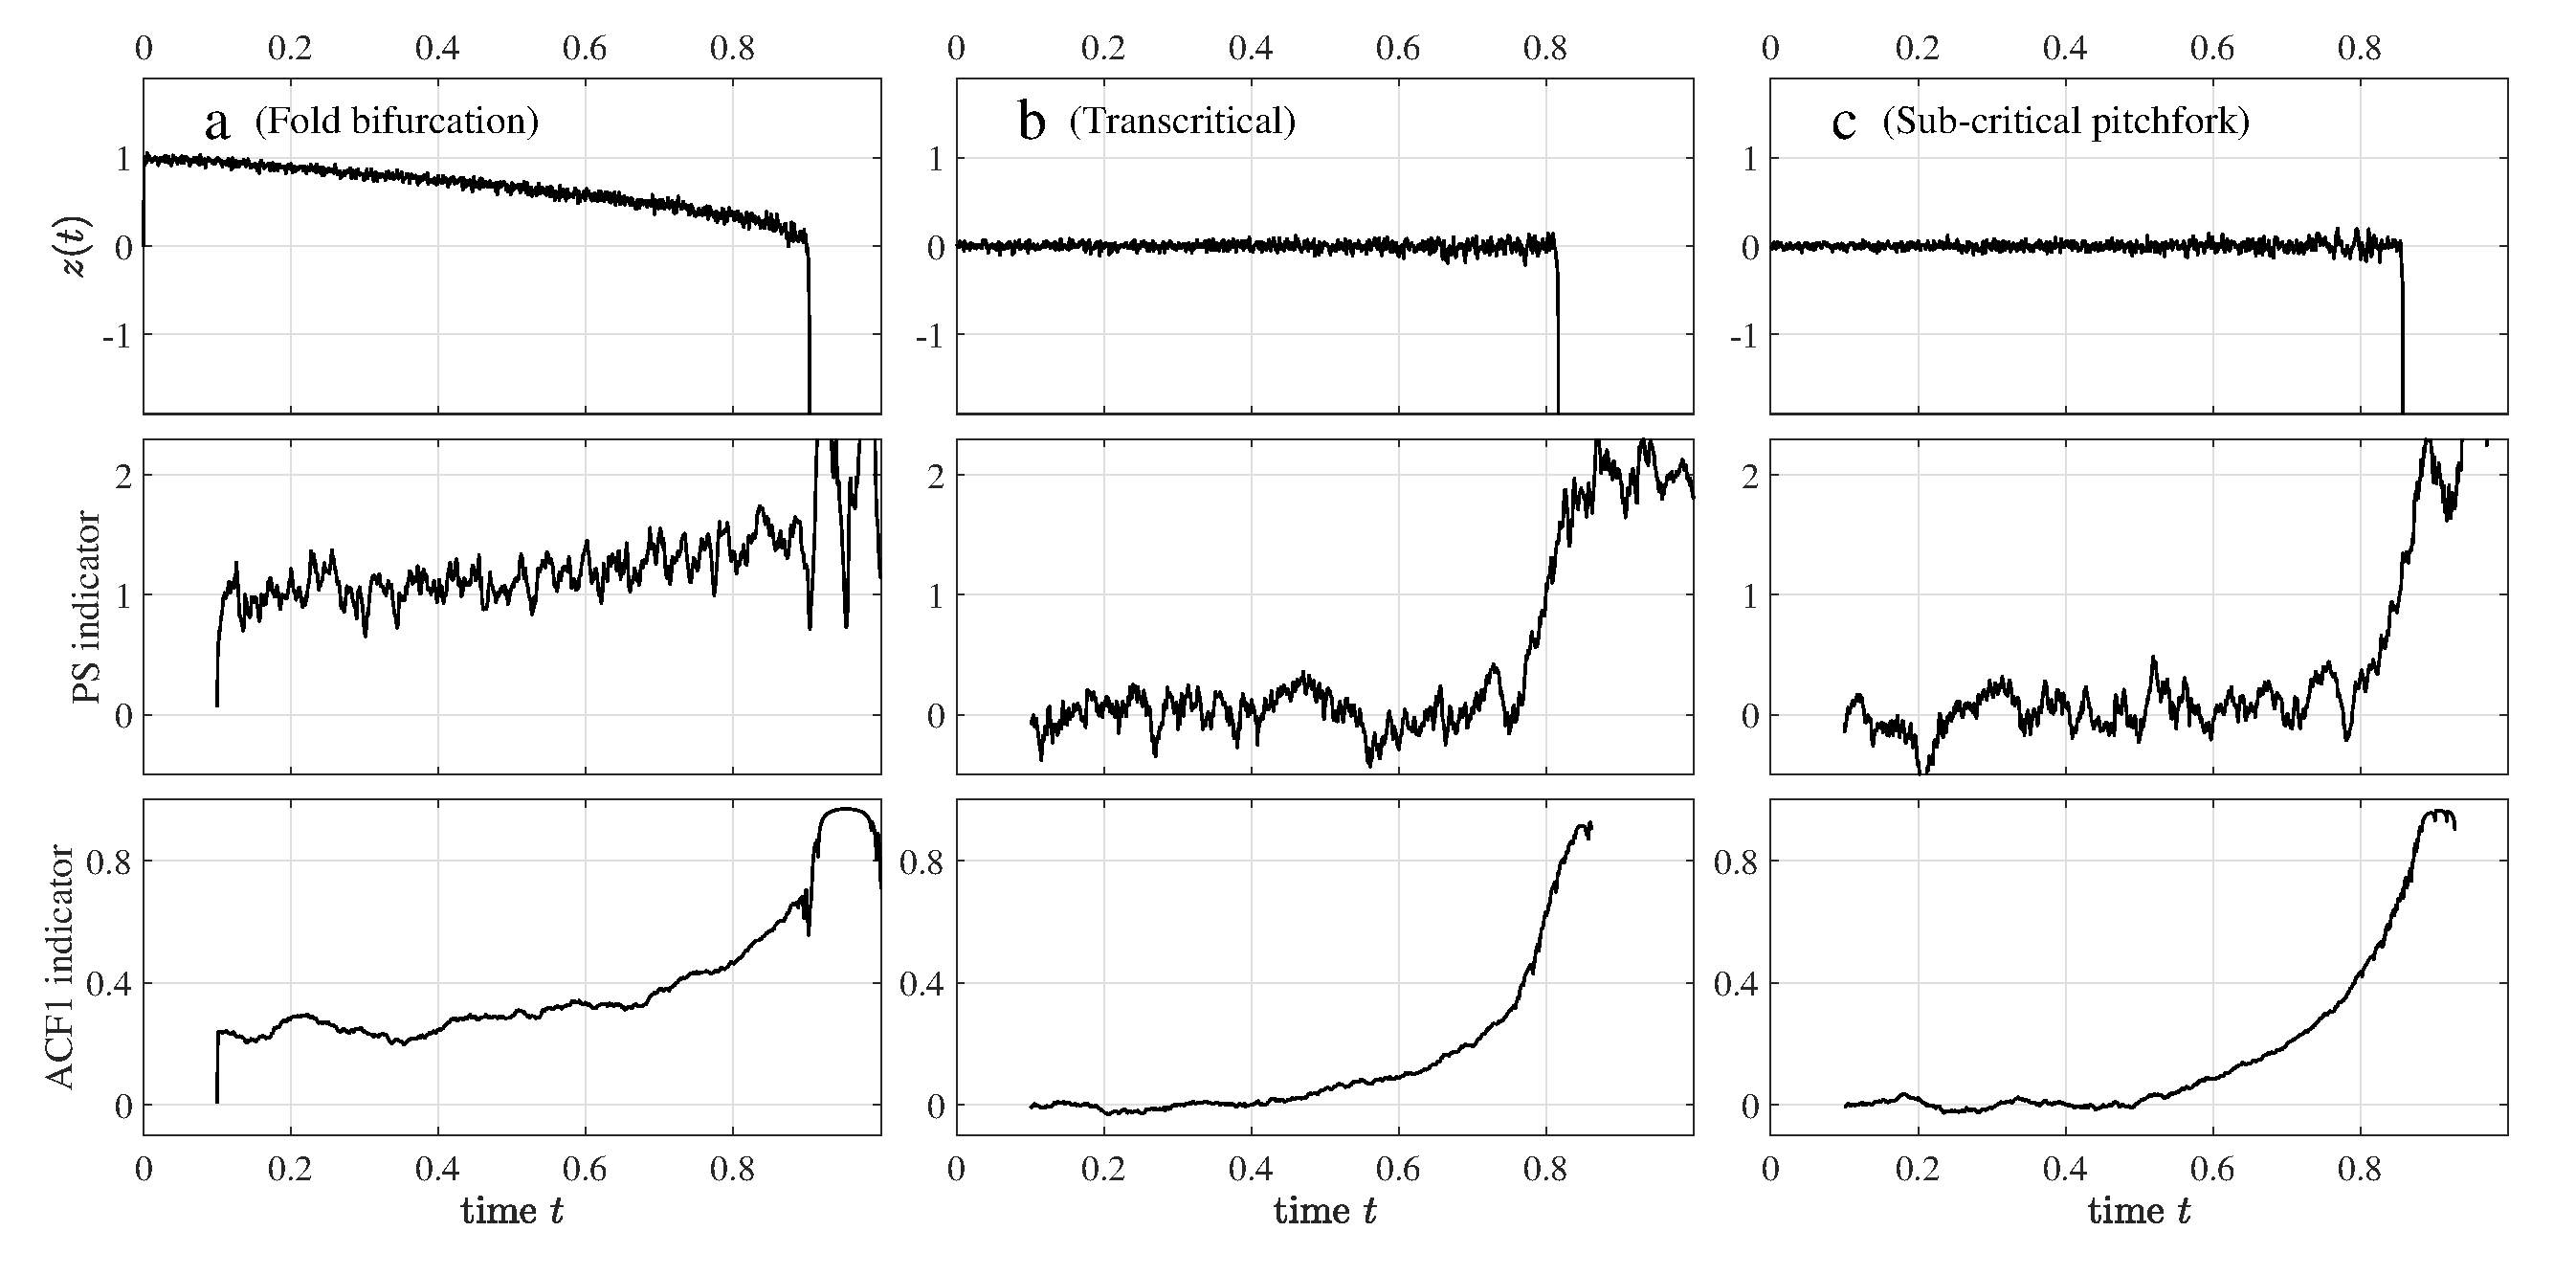
\includegraphics[width=\linewidth,keepaspectratio]{bifurcations30}
		\caption{\Red{Three systems given by equations~\ref{eqn:1D:TypesOfBifurcation:fold} (fold bifurcation), \ref{eqn:1D:TypesOfBifurcation:transcritical} (transcritical bifurcation), and \ref{eqn:1D:TypesOfBifurcation:sub-critical} (sub-critical pitchfork bifurcation) are integrated between $t=0$ and $t=1$. Each exhibits a bifurcation at around $t=0.9$: a fold, transcritical, and sub-critical pitchfork bifurcation (panels {\bf a}, {\bf b}, {\bf c} respectively). The PS and ACF1 indicators are calculated using a sliding window of 100 points and plotted beneath the time series for each system. We note the similarity in shape between the two indicator signals, although the PS indicator is more noisy. }
		}
		\label{fig:1D:TypesOfBifurcation:threesystemswithPSandACF}
	\end{figure}
\end{landscape}

\subsection{Early warning signals for three bifurcational tipping points}
\label{subsec:1D:indicatorComparison:TypesOfBifurcation}

{\Red
	In section~\ref{sec:intro:bifurcation_varieties}, chapter~\ref{chap:intro}, we presented three examples of dynamical systems each exhibiting a different bifurcation implying a tipping point: a fold bifurcation, a transcritical bifurcation and a sub-critical pitchfork bifurcation.
	
	We give the equations for each of these three examples again here. In each case the system equation is in the `generalised potential' form of equation~\ref{eqn:1D:numerical_integration:potentialform} and integrated numerically using the Milstein method (see section~\ref{sec:1D:numerical_integration}, page~\pageref{sec:1D:numerical_integration}) with time step $\Delta t = 10^{\m 5}$ and a sampling rate of $10^3$ per unit time. Thus each integration generates a time series of $1000$ points since the time range in each case is $t\in [0,1]$. The results of all three experiments are shown in figure~\ref{fig:1D:TypesOfBifurcation:threesystemswithPSandACF}
	
	\subsubsection{Type 1: Fold bifurcation}
	The fold bifurcation is a very simple example of a tipping point and has been used to model a wide variety of phenomena, notably in the field of \emph{catastrophe theory} \citep{zeeman1977catastrophe, arnold1999bifurcation}. We consider a dynamical system given by the equation
	\begin{equation}
	\label{eqn:1D:TypesOfBifurcation:fold}
		\dot{z}(t) = -\frac{\partial }{\partial z}\left(z^3+\frac{(10t-9)}{3}z\right),
	\end{equation}
	where $\mu = (10t-9)/3$ is the model parameter. The bifurcation occurs at $\mu=0$, $t=0.9$ when the stable equilibrium at $z=\m\sqrt{\mu/3}$ meets the unstable equilibrium at $z=+\sqrt{\mu/3}$. After this point the system `blows up' since $z$ diverges to infinity. In figure~\ref{fig:1D:TypesOfBifurcation:threesystemswithPSandACF}a we see that both the PS and ACF1 indicators show an increasing trend before the bifurcation occurs, but in the PS indicator this is barely noticeable. 


	
	\subsubsection{Type 2: Transcritical bifurcation}
	The transcritical bifurcation is so named because the equilibria \emph{cross} the critical point: they are not created nor eliminated. Instead, the stable equilibrium becomes unstable and \emph{vice versa}. The normal form of the transcritical bifurcation is
	\begin{equation}
	\dot{z}(t) = -\frac{\partial }{\partial z}\left(z^3-\mu z^2\right),
	\label{eqn:1D:TypesOfBifurcation:transcritical}
	\end{equation}
	which has the same (cubic) shaped generalised potential function as the fold bifurcation normal form. When $\mu=0$, this example has a stable equilibrium at $z = 2\mu/3$ and an unstable equilibrium at $z=0$. At the critical point $\mu=0$ the equilibria are lost momentarily but reappear for $\mu>0$ when the $z=0$ state has become unstable and the (positive) $z = 2\mu/3$ state is now stable. Because of the continuity of the equilibrium at $z=0$, this type of equation is used frequently in biology when zero is often a stable state \citep{nicolis2007,strogatz2014}, for example in population dynamics (of bacteria, humans, etc.) a population of zero is a stable population. Indeed, the above equation has the same form as the logistic equation \citep{brown2018introduction}. In figure~\ref{fig:1D:TypesOfBifurcation:threesystemswithPSandACF}b we see, again, that the ACF1 and PS indicators have a similar shape but that the PS indicator is more noisy and the increasing trend is not visible until closer to the tipping point.
	
	\subsubsection{Type 3: Sub-critical pitchfork bifurcation}
	We have seen already the super-critical pitchfork bifurcation, equation~\ref{eqn:1D:DifferentTypesOfTipping:genuine}, used as an example of a genuine bifurcation in comparison to other types of tipping points (see figure~\ref{fig:1D:threesystemswithPSandACF}b). The contrasting \emph{sub}-critical pitchfork bifurcation has the normal form
	\begin{equation}
	\label{eqn:1D:TypesOfBifurcation:sub-critical}
	\dot{z}(t)  = -\frac{\partial}{\partial z}\left(\m z^4 - \mu z^2\right),
	\end{equation}
	and for $\mu<0$ has a single stable equilibrium at $z=0$ and two unstable equilibria at $z=\pm\sqrt{\m\mu/2}$. At the critical point $z=0$ the two unstable equilibria meet the stable point and develop into a single unstable equilibrium for $\mu>0$. Thus, a system following the stable trajectory will abruptly become unstable at the critical point and quickly diverge to $\pm\infty$ given any small perturbation. Of course, in cases with higher order terms in the equation, the system may in fact converge again to a separate stable point away from $z=0$. As with the fold bifurcation, we see in figure~\ref{fig:1D:TypesOfBifurcation:threesystemswithPSandACF}c that the ACF1 and PS indicators have a similar shape but that the PS indicator is more noisy and the increasing trend is not visible until closer to the tipping point.

	
}

\subsection{The supercritical pitchfork bifurcation model}
 \label{subsec:1D:indicatorComparison:PitchforkModel}

{\Red{
		\subsubsection{Indicators applied}
		We have already looked at a dynamical system experiencing a supercritical pitchfork bifurcation (see figure~\ref{fig:1D:threesystemswithPSandACF}b, page~\pageref{fig:1D:threesystemswithPSandACF}) in comparison to other types of tipping points, and we have seen how well the PS indicator provides an EWS for this system in comparison with the ACF1 indicator. In this section we look more closely at the result in figure~\ref{fig:1D:threesystemswithPSandACF}b and also calculate the EWS given by the DFA indicator. In addition, we address the problem of \emph{predicting}, rather than merely detecting, a tipping point, using this dynamical system as our example.
The dynamical system is, as in section~\ref{subsec:1D:indicatorComparison:TypesOfTipping}, given by the equation
	\begin{equation}
	\label{eqn:1D:EWS:Pitchfork}
		\dot{z}(t) = -\frac{\partial }{\partial z}\left(z^4-(5t-3)z^2\right) + \frac{1}{10}\eta\,,
	\end{equation}
where $\mu=(5t-3)$ is our model parameter and the bifurcation occurs at $\mu=0\Rightarrow t=0.6$. For $\mu<0$ the system has a single stable equilibrium at $z=0$. This becomes unstable for $\mu>0$ and two new stable points develop at $z = \pm\sqrt{\mu}$. }}

\begin{figure}
	\centering
	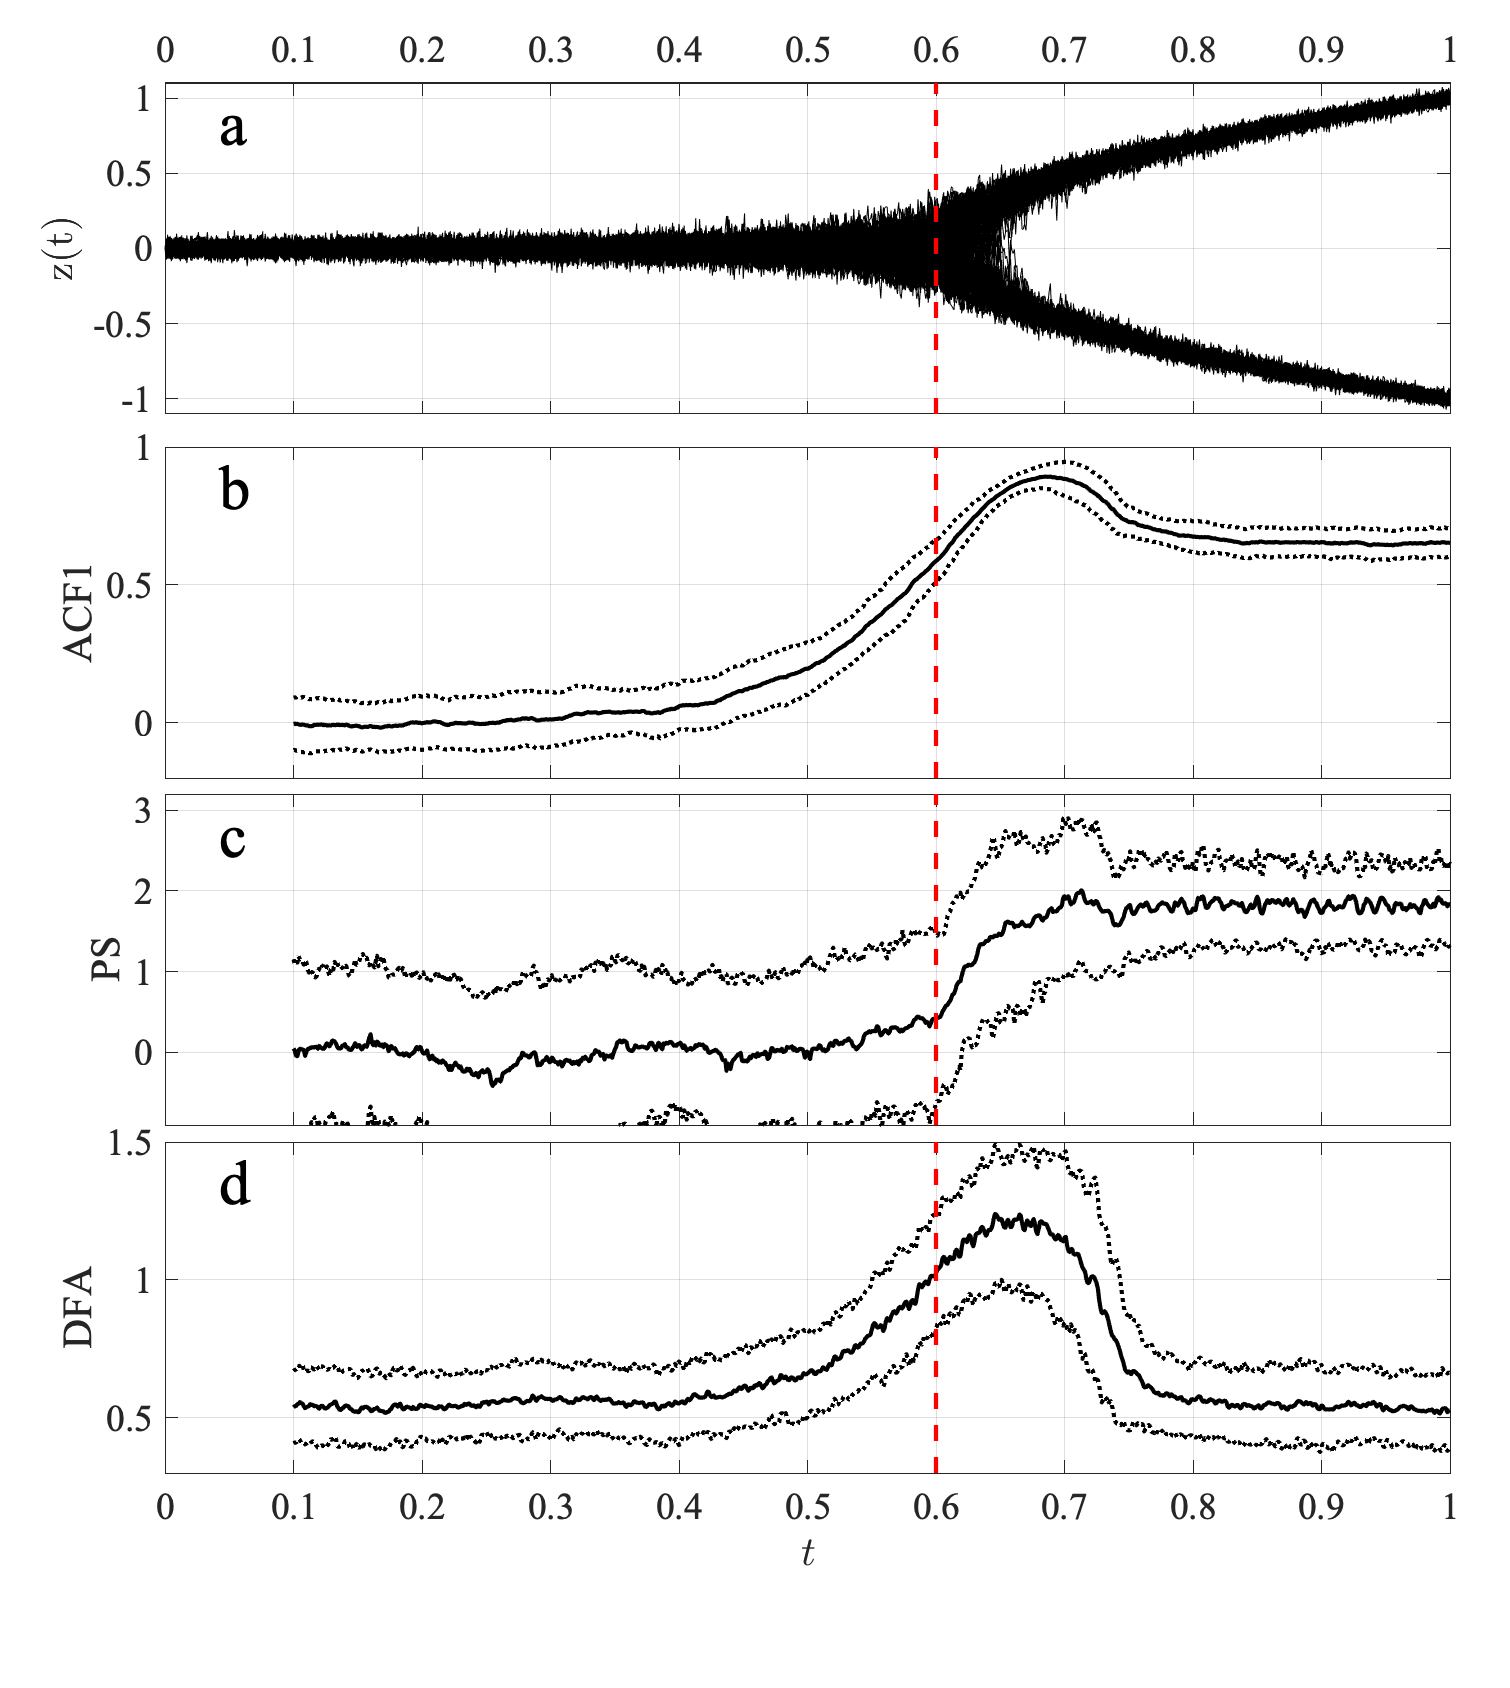
\includegraphics[width = 0.9\textwidth]{pitchforkEWS}
	\caption{\Red{ACF1, PS and DFA indicators applied to time series of the pitchfork bifurcation model. Panel {\bf a}: Data from an ensemble of $100$ runs of the model (see equation \ref{eqn:1D:EWS:Pitchfork}); Panels {\bf b}, {\bf c}, {\bf d}: The mean ACF1, PS and DFA indicators (all using window size 100) shown with error bars of one standard deviation.
	}}
	\label{fig:1D:pitchforkEWS}
\end{figure}

{\Red{Equation \ref{eqn:1D:EWS:Pitchfork} is integrated numerically with a time step of $\delta t =10^{\m5}$, from $t=0$ to $t=1$, and sampled at a rate of $10^3$ points per unit time to give a time series of length $N=10^3$. The ACF1, PS and DFA indicators are then applied with a window size of 100 points. This experiment is repeated for 100 such time series and the indicators are applied to all of them. The means of the indicator series are found and are plotted in figure~\ref{fig:1D:pitchforkEWS} with error bounds of one standard deviation.
		
We see that the ACF1 and DFA both provide an EWS, beginning to show a clear increasing trend at around $t=0.4$. The PS indicator, however, does not show a convincing trend (in the mean) until after the bifurcation has occurred, and the trend is not significant when the error bounds are taken into consideration. We do see that the PS indicator series shows a similar general shape to the ACF1 indicator: after increasing to a maximum value, both settle down to a constant value that is closer to that of red noise than white noise, whereas the DFA indicator settles back to a white-noise value ($0.5$ for DFA) after the bifurcation. The reason for the high value of the PS and ACF1 indicators after the bifurcation, although the system is trapped around a single stable point, much like before the bifurcation, is that the parabolic trend in the post-bifurcation system biases the autocorrelation whilst the detrending step in the DFA algorithm removes this and views both `single equilibrium' stages of the system equally. This is consistent with the findings presented in figure~\ref{fig:1D:PSsensitivity_trend} (page~\pageref{fig:1D:PSsensitivity_trend}), where both the PS and ACF1 indicators were biased by imposing a parabolic trend onto the AR(1) model when using a time series of $100$ points. Since the window size used for our experiment here was also $100$ points, we would expect the same result. For a window size of $10^5$ points we would expect (based on figure~\ref{fig:1D:PSsensitivity_trend}) that the PS indicator would not show bias. Given the highly variable performance of the PS indicator in that previous experiment, it is somewhat surprising that we any trend, even in the mean over an ensemble of $100$. 
}}


\begin{figure}
	\centering
	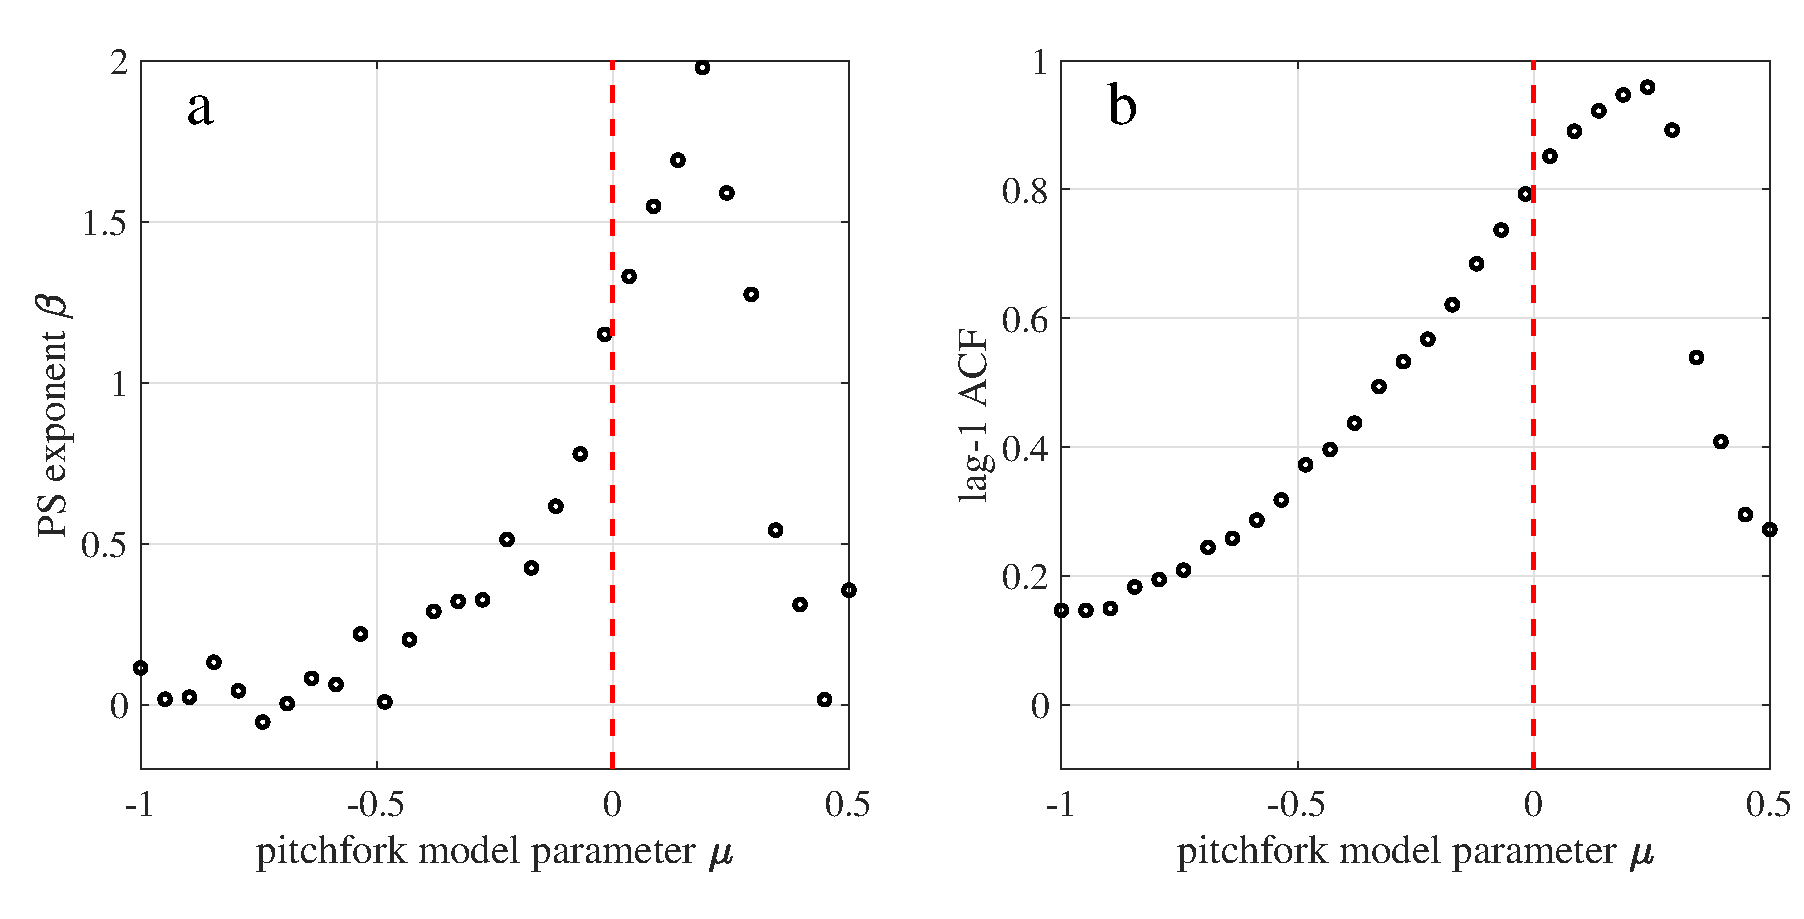
\includegraphics[width = 0.9\textwidth]{pitchforkMuRelationship}
	\caption{\Red{$30$ time series of length $10^5$ are created by integrating equation~\ref{eqn:1D:EWS:Pitchfork} using a \emph{constant} parameter $\mu$. Each time series uses a different constant value of $\mu$ between $\m1$ and $0.5$. The PS exponent (panel {\bf a}) and lag-1 autocorrelation (panel {\bf b}) are calculated for each time series.}}
	\label{fig:1D:pitchforkMuRelationship}
\end{figure}

{\Red{
		\subsubsection{Further experimentation}
		In order to further understand the relationship between the PS exponent and the parameter of the pitchfork model, we perform a more detailed experiment. In this case we use time series of length $10^5$, in order to see if significantly alters the results of the PS indicator, as was the case with the AR(1) model (see section~\ref{subsec:1D:Exponents_as_EWS:PSsensitivity}). 
		
		$30$ time series of length $10^5$ are created by integrating equation~\ref{eqn:1D:EWS:Pitchfork} using a \emph{constant} parameter $\mu$. Each time series uses a different constant value of $\mu$ between $\m1$ and $0.5$. The PS exponent and lag-1 autocorrelation are calculated for each time series. The results are shown in figure~\ref{fig:1D:pitchforkMuRelationship}. We see the same shape as in figure~\ref{fig:1D:pitchforkEWS}, with the values of the two indicators were plotted over time. Certainly the PS exponent are similarly related to the parameter of this pitchfork system just as they are for the AR(1) model, although there is much lower error involved in using the lag-1 ACF.
	}}

%\subsection{Early warning signals in the ??? system}
%\label{sec:1D:VanderPol}

%We now apply the 




\section{Discussion}
\label{sec:1D:discussion}

We have developed a novel indicator of EWS for tipping points in dynamical systems by estimating the power-law decay rate of the power spectrum in a sliding window \citep{prettyman2018}. {\Red{The PS exponent has been shown analytically to provide an indication of critical slowing down (see section~\ref{subsec:1D:Exponents_as_EWS:indicators}) based on the model of critical slowing down as an AR(1) process, and therefore the PS indicator is expected to provide an EWS of tipping points in the same way that the ACF1 and DFA indicators have previously been used.}} We have applied this PS indicator, along with the ACF1 and DFA indicators, to several different time series of models of various tipping points, including various bifurcations and non-bifurcational tipping. 

We have found that the PS indicator behaves similarly to the previously used ACF1 and DFA indicators applied to the model data, but with larger variance, which limits its usefulness in situations where the model has a noisy trajectory or cannot be observed multiple times.

Of the ACF, DFA and PS scaling exponents, all may be used as EWS indicators, although \citet{kantelhardt2001} notes that a direct calculation the ACF exponent $\gamma$ is often unsuitable and the DFA method is therefore introduced as an indirect measure. In our own implementations of the two methods, the ACF exponent is less reliable. The less computationally expensive lag-1 autocorrelation function is also often used instead of the ACF exponent since both provide a measure of critical slowing down (see equation \ref{eqn:1D:AR1_decay_model}), but it is highly sensitive to trends and periodicity. {\Red In contrast, the PS indicator is relatively insensitive to periodicity, as we have demonstrated in section~\ref{subsec:1D:Exponents_as_EWS:Periodicity} (page~\pageref{subsec:1D:Exponents_as_EWS:Periodicity}). The addition of a simple periodic function to an AR1 process does not affect the value of the PS exponent even whilst the lag-1 autocorrelation and DFA exponent are significantly affected so as to make the estimation of the model parameter (the critical slowing down proxy) impossible.}

\cite{heneghan2000} notes that the DFA and PS exponents have a predictable relationship and therefore the use of both is not necessary. {\Red{ However, this is true only when power-law scaling exists and does not hold when there is a cross-over in the power spectrum as demonstrated by the comparison in figure~\ref{fig:1D:ExponentRelationships}, nor may it be the case in oscillating systems. The choice between the two techniques may therefore be important when investigating tipping points, and the study of the behaviour of the PS exponent may reveal trends in the data which a study using the DFA or ACF exponents may not.}}

%!TEX root = ../thesis.tex

\chapter[Multivariate tipping point techniques]{Extension of tipping point techniques to multivariate data}
\label{chap:2D}

\graphicspath{{Chap_Multivariable/Figs/}}

    	Early warning signal techniques generally are applied only to univariate data, often one-dimensional time series from a single data source or model output. In an effort to study multidimensional geophysical variables we here consider cases where we have more than one time series, either because
    	\begin{enumerate}
    		\item there are multiple measured variables,
    		\item a variable is measured at multiple spacial locations,
    		\item both of these simultaneously.
    	\end{enumerate}  
    	In the first case it may suffice to attempt an EWS detection on each time series individually, but one can envision a scenario where it is possible to detect an EWS in neither $X(t)$ nor $Y(t)$ but, considered together in some way, an EWS is detectable. It may therefore be worthwhile to investigate the possibility of an analogue to existing one-dimensional tipping point techniques for time series in two or more variables. In the case of gridded data it is common to use Empirical Orthogonal Functions (EOF), also known as Principal Component Analysis (PCA), to reduce the dimensionality of a system \citep{vonstorch,jolliffe1986}. This technique has also been more specifically applied to EWS methods \citep{held2004,bathiany2013p1,kwasniok2018}. Principal interaction and oscillation patterns (PIPs and POPs) can be considered as extensions of the EOF method and provide additional techniques for the dimension reduction of complex systems \citep{hasselmann1988}.
    	
  		It has been suggested that an EWS is detectable in a dynamical system defined over a two-dimensional field, such as climatological or ecological variable modelled or measured at multiple geographical points \citep{guttal2009spatial, donangelo2010early, dakos2010spatial}. There has been a large amount of work involving the use of multiple data sources spread over a geographic area, such as complex network analysis in climatology \citep{tsonis2006,yamasaki2008,gozolchiani2011} which has been applied to the El Ni{\~n}o. In these suggested methods, the cross-covariance or cross-correlation is calculated between points on a grid, rather than the temporal autocorrelation (or related properties) being calculated. The assumption here is that the correlation between neighbouring points will increase close to a tipping point. Similar techniques calculate the cross-covariance of a variable, at a specific time slice, between points inside a specified region of interest \citep{ludescher2013,ludescher2014} or identify emerging spatial patterns in the data \citep{kefi2014early}. It is also possible to identify regions of interest, or "hotspots": \citet{bathiany2013p1} partition the field into elements and use EOFs to determine which elements contribute most to the autocorrelation. The method is applied successfully to a highly idealised model of a vegetation cover.
    	
    	In this chapter we review and analyse techniques which may be used to calculate an EWS with an input of two variables, namely the methods presented by \citet{williamson2015} (in section~\ref{sec:2D:Williamson}), and the use of EOFs for dimension-reduction (in section~\ref{sec:2D:EOF}). These two techniques are applied, in section~\ref{sec:2D:MethodsApplied}, to multivariate time series data from models of three simple dynamical systems: two are examples taken from \citet{williamson2015}, and the results are successfully reproduced; the third example is the Van der Pol oscillator, which allows us to test the same methods in a novel system. In chapter~\ref{chap:cyclones} these same methods will be applied to real measurements of physical variables, alongside the one-dimensional techniques (see chapter~\ref{chap:1D}). 
    	
    	In section~\ref{sec:2D:EOF-justification} the method of using EOF for dimension reduction prior to the application of an EWS indicator is tested analytically, thus providing a step towards a mathematically rigorous understanding of the commonly used method. In section~\ref{sec:2D:AlternativeEOF} we present an alternative formulation of the EOF method for dimension reduction. 
  	
    	In section~\ref{sec:2D:ExtensionToGridded} we present a method to visualise early warning signals in a dynamical system over a 2D field, and apply this method to data from a simple model of a progressing "front", in which the variable is modelled at discrete grid points. Again, in chapter~\ref{chap:cyclones}, this method will be applied to real measured physical variables, that is, the  time series of geophysical variables measured at geographically separated locations in the vicinity of an approaching tropical cyclone with monitoring of sea-level pressure.
    	
    	

\section{Multivariate extension of the autocorrelation function}
\label{sec:2D:Williamson}

\citet{williamson2015} introduce a method to anticipate bifurcations in dynamical systems with more than one variable. The method is a higher-dimensional analogue of the one-dimensional ACF1 indicator. Indeed, we note the similarities between the equation used to calculate the lag-1 autocorrelation coefficient $a$ in the one dimensional time series $\{x_t\}$:
\begin{equation}
	a = \frac{   \sum_t (x_{t+1}x_t)   - \overline{x}^2}{\sum_t (x_t^2) - \overline{x}^2}\,,
	\label{eqn:2D:williamson-1Dautocorrelation}
\end{equation}
and the equation given by the authors:
\begin{equation}
	A = \left[\sum_t (\x_{t+1}\x_t^\top)   - \overline{\x}^2\right]\left[\sum_t (\x_t\x_t^\top) - \overline{\x}^2\right]^{-1}\,,
	\label{eqn:2D:williamson-autoA}
\end{equation}
where $\{\x_t\}$ is a multivariate time series. By linearising and discretising, one may approximate the one-dimensional time series $\dot{x} = f(x) + \eta(t)$ as the auto regressive system
\begin{equation}
x_t = ax_{t-1} + c + \eta_t,
\label{eqn:2D:williamson-AR1equation}
\end{equation}
where $c$ is a scalar value and $\eta_t$ is Gaussian noise. An AR(1) model of a system may therefore be constructed based only on time series data, by calculating the parameter $a$ using equation \ref{eqn:2D:williamson-1Dautocorrelation}, that is, the lag-1 autocorrelation coefficient. In the same way, the matrix $A$ may be used to model an $N$-dimensional system $\dot{x}^{(i)} = f(x^{(1)},...,x^{(N)})+\eta^{(i)}$ using the analogous form
\begin{equation}
\x_t = A\x_{t-1} + \mathbf{c} + \mathbf{\eta}_t,
\label{eqn:2D:williamson-AR1analogue}
\end{equation}
where $\mathbf{c}$ is a constant vector and $\mathbf{\eta}_t$ is a vector with each element being an independent Gaussian white noise term. In this linear system a tipping point occurs when an eigenvalue of $A$ has the value one. It is, therefore, changes in the eigenvalues of $A$ that must be studied and these are calculated easily once the matrix $A$ has been found from time series data, according to equation~\ref{eqn:2D:williamson-autoA}. However, it is more useful to study the eigenvalues of the Jacobian of the system equations, since their behaviour is already well studied in many contexts. For example, a Hopf bifurcation is characterised by a conjugate pair of Jacobian eigenvalues crossing the imaginary axis \citep{strogatz2014}. Tracking the changes in the imaginary part of one of these eigenvalues as it approaches zero therefore gives an early warning signal of the Hopf bifurcation. 

Given a system of equations, for example the two-dimensional system
	\begin{equation}
		\begin{array}{rcl}
			\dot{x}&=&f(t,x,y),\\
			\dot{y}&=&g(t,x,y),
		\end{array}
	\end{equation}
which has a stable centre at the point $\mathbf{x}_\star=(x_\star, y_\star)$, we can calculate the Jacobian matrix explicitly, evaluated at $\mathbf{x}_\star$:
	\begin{equation}
		J(\mathbf{x}_\star) = \left(\begin{array}{cc}
		\left. \frac{df}{dx}\right|_{\mathbf{x}_\star} & \left. \frac{df}{dy}\right|_{\mathbf{x}_\star}\\
		~\\
		\left. \frac{dg}{dx}\right|_{\mathbf{x}_\star} & \left. \frac{dg}{dy}\right|_{\mathbf{x}_\star}
		\end{array}\right).
	\end{equation}
This allows us to study the effect of a small perturbation in $x$ or $y$ and, as noted, the eigenvalues of the Jacobian matrix are well studied in many dynamical systems \citep{thompson2002nonlinear}.

However, we are interested in detecting and anticipating tipping points in time series, not analytically defined systems. \citet{williamson2015} provide a method for estimating the eigenvalues $\lambda_k$ of the Jacobian, given a time series. Rather than attempting to calculate the $\lambda_k$ from a time series, the authors calculate the matrix $A$ directly using equation \ref{eqn:2D:williamson-autoA} and then refer to the discretised system (equation~\ref{eqn:2D:williamson-AR1analogue}), in which $A = \mathbf{I}+J(\mathbf{x}_\star)\Delta t$. The first order approximation 
	\begin{equation}
		A = \mathbf{I}+J(\mathbf{x}_\star)\Delta t \approx \exp(J(\mathbf{x}_\star)\Delta t)
		\label{eqn_jacobian_justification}
	\end{equation}
is used to recover the Jacobian eigenvalues $\lambda_k$ from the eigenvalues $a_k = |a_k|\exp(i\varphi)$ of $A$, with the relations 
	\begin{align}
		\begin{split}
			\mathbb{R}(\lambda_k) &= \frac{1}{\Delta t}\ln|a_k|\,,\\
			\mathbb{I}(\lambda_k) &= \frac{1}{\Delta t} \varphi_k\,.
		\end{split}
		\label{eqn:2D:williamson-eigenvalueRelations}
	\end{align}
The eigenvalues $\lambda_k$ are then, themselves,  tipping point indicators. To obtain an EWS, the method then involves calculating the matrix $A$ from the given time series data in a sliding window, similarly to the one-dimensional ACF1 indicator, and recovering the Jacobian eigenvalues using equation~\ref{eqn:2D:williamson-eigenvalueRelations}.

We note that this method is only effective as an EWS if the type of expected tipping, particularly a bifurcation, is known in advance, since it is necessary to know which eigenvalue to study in order to use that eigenvalue as an indicator. However, an obvious increase or decrease in either eigenvalue may provide an indication that a critical transition is happening, and could therefore lend confidence to an EWS derived by another method. The method, however, would certainly be useful in the detection and classification of tipping points, when applied retrospectively. In systems of more than two variables the situation is more acute because of the increased number of eigenvalues. Identifying conjugate pairs may lead to some insight as to which could be indicators (depending of the type of bifurcation), and will reduce the number of distinct eigenvalues. 

\subsubsection{Analysis of a Hopf bifurcation}
In order to analyse this method further we take, as an example, the Van der Pol oscillator 
	\begin{equation}
		\begin{array}{rcl}
			\dot{x} &=& \mu\left(x - \frac{1}{3}x^3\right)+y,\\
			\dot{y} &=& -x,
		\end{array}
	\label{eqn:2D:exampleVDP}
	\end{equation} 
which experiences a Hopf bifurcation at $\mu=0$ if $\mu$ varies. That is, the eigenvalues are a complex conjugate pair whose imaginary parts cross the imaginary axis at $\mu=0$ \citep{strogatz2014}. In section~\ref{sec:2D:MethodsApplied} we shall integrate this system numerically with added noise and apply the EWS method described here to the resulting time series. Here we consider only the analytic process of the method.

We see that the system has a stable point at $\mathbf{x}_\star=(0,0)$ and the Jacobian is found to be
	\begin{equation}
		J(\mathbf{x}_\star) = \left.\left(
		\begin{array}{cc}
		\mu(1-x^2) & 1\\
		-1 & 0
		\end{array}
		\right)\right|_{(0,0)} = \left(
		\begin{array}{cc}
		\mu & 1\\
		-1 & 0
		\end{array}
		\right) \,,
	\label{eqn:2D:exampleVDPJacobian}
	\end{equation}
with eigenvalues
	\begin{align}
		\lambda &=\frac{1}{2}\left(\mu\pm\sqrt{\mu^2-4}\right)\\
		&= \frac{\mu}{2}\pm i~ \frac{\sqrt{4-\mu^2}}{2}~~~~~ \text{where}~|\mu|<2\,.
	\label{eqn:2D:VDPactualJacobianEigenvalues}
	\end{align} 
We obtain the matrix $A$ by discretising according to the Euler method:
	\begin{align}
		\left(\begin{array}{c}
		x_{t+1}\\y_{t+1}
		\end{array}\right) &= \left(\begin{array}{c}
		x_{t}\\y_{t}\end{array}\right) + \Delta t \left(\begin{array}{c}
		\mu(x_{t}-x_{t}^3/3)+y_{t}\\
		-x_{t}
		\end{array}\right).
	\end{align}
We use the linearisation $x^3=0$ to continue:
	\begin{align}
		\left(\begin{array}{c}
		x_{t+1}\\y_{t+1}
		\end{array}\right) &= \left(\begin{array}{c}
		x_{t}\\y_{t}\end{array}\right) + \Delta t \left(\begin{array}{c}
		\mu x_{t} +y_{t}\\
		-x_{tt}
		\end{array}\right)\\
		&= \left(\begin{array}{cc}
		1 + \Delta t \mu & \Delta t\\
		-\Delta t & 1
		\end{array}\right) \left(\begin{array}{c}
		x_{t}\\y_{t}\end{array}\right).
	\label{eqn:2D:AnalyticMatrixA}
	\end{align}
The matrix in equation~\ref{eqn:2D:AnalyticMatrixA} is the matrix $A$, with eigenvalues 
	\begin{equation}
		a = \frac{2+\Delta t \mu}{2} \pm i~ \frac{\Delta t \sqrt{4-\mu^2}}{2} ~,~~~~\text{where}~|\mu|<2\,.
	\end{equation}
Or $a = |a|\exp(i\varphi)$, where
	\begin{equation}
		\begin{array}{ccc}
		|a| &=& \sqrt{\Delta t^2 + \Delta t \mu +1}\,,\\
		\varphi &=& \arctan\left(\frac{\Delta t \sqrt{4-\mu^2}}{2+\Delta t}\right)\,.
		\end{array}
	\end{equation}
These eigenvalues of $A$ can now be used to reconstruct the eigenvalues of the Jacobian. Referring to equations~\ref{eqn:2D:williamson-eigenvalueRelations}, and using the power series expansions \(\arctan(x) = x - x^3/3 +...\) and \(\ln(x+1) = x-x^2/2+...\)\, , we find
	\begin{align}
		\mathbb{R}(\lambda) &= \frac{1}{\Delta t}\ln|a| = \frac{\mu}{2} + \frac{\Delta t}{2} + \Delta t\frac{\mu^2}{4} + \mathcal{O}(\Delta t^2)\,,\\
		\mathbb{I}(\lambda) &= \frac{1}{\Delta t} \varphi = \frac{\sqrt{4-\mu^2}}{2+\Delta t} + \mathcal{O}(\Delta t^2)\,.
	\label{eqn:2D:EstimatedLambdaVDP}
	\end{align}
If we use the approximation $\Delta t =0$, which is valid for very small $\Delta t$, these agree exactly with the Jacobian eigenvalues found in equation~\ref{eqn:2D:VDPactualJacobianEigenvalues}. Thus, from the linearised system $\mathbf{x}_{t+1}=A\mathbf{x}_t$ in equation~\ref{eqn:2D:AnalyticMatrixA}, we have reconstructed the Jacobian eigenvalues, evaluated at the stable centre, of the non-linearised system (equation~\ref{eqn:2D:exampleVDP}), with only the assumption that $\Delta t$ is close to zero. 


\section{Dimension reduction using EOFs}
\label{sec:2D:EOF}

In this section we study the technique of dimension reduction using empirical orthogonal functions (EOFs), also known as principal components analysis. This technique is widely used in geosciences and meteorology to aid the study of a large, multivariate data set \citep{bjornsson1997,stephenson2000}. \citet{held2004} use the EOF technique prior to applying the ACF1 indicator to a set of gridded time series, relying on the observation that an increase in autocorrelation is typically accompanied by an increase in variance. \citet{held2004} use this observation to argue that in a multi-dimensional system one should project onto the first EOF (the basis vector for which the variance of the system is maximised) as this is the one-dimensional basis in which the rise in autocorrelation (and also variance) will occur. 

We note that the basis in which the variance is maximal may not be the same as the basis in which the variance is increasing. At least, this is not obvious {\it a priori}. In some dynamical systems it may be that while autocorrelation rises before a tipping point, variance does not \citep{livina2012, gsell2016}. This observation is investigated further in section~\ref{sec:2D:EOF-justification}.

In this section we explain the EOF method for dimension reduction. In section~\ref{sec:2D:MethodsApplied} we apply this method to three two-variable time series prior to using the one-dimensional ACF1, DFA and PS indicators. 

\subsection{Empirical orthogonal functions}
\label{subsec:2D:EOF:description}

The EOF method involves projecting a data matrix $Y$ of $N$ time series onto a different basis to obtain $N$ new time series. This basis is orthogonal and is constructed so that projecting $Y$ onto the first basis vector maximises the variance of the projection. The second basis vector is such that projecting $Y$ onto it will maximise the variance given that it must be orthogonal to the first, and so on. Thus, the first one or two EOF scores may capture most of the variance of the whole data set of hundreds of time series. 

We consider $N$ observations  $\x_1, \x_2, ..., \x_N$ of a $P$-dimensional system, collected in the $N\times P$ matrix $X$, shown in equation \ref{eqn:EOF-matrixX}.
	\begin{equation}
		X = \begin{bmatrix}
		\x_1^\top  \\
		\vdots \\
		\x_N^\top 
		\end{bmatrix}
		= \begin{bmatrix}
		x_{11} & \hdots & x_{1P} \\
		\vdots & \ddots & \vdots \\
		x_{N1} & \hdots & x_{NP} 
		\end{bmatrix}.
	\label{eqn:EOF-matrixX}
	\end{equation}
The method requires a mean-centred series so it is common to replace the series $[\x_n]_{n=1}^N$ with a new set of series $[\y_n]_{n=1}^N$, were the $i\textsuperscript{th}$ element of $\y_n$, which we call $\y_n^{(i)}$, is given by
	\begin{equation}
	\y_n^{(i)} = \x_n^{(i)} - \frac{1}{N}\sum_{j = 1}^N \x_j^{(i)},
	\end{equation}
	 %The matrix $Y$ is then created where the $(N-n)\textsuperscript{th}$ row is the row vector $\y_n^\top$. 
so that a new matrix $Y$ is created from the $N$ time series $\y_1, \y_2, ..., \y_N$, similar to the matrix $X$ in equation \ref{eqn:EOF-matrixX}.
We then project $Y$ onto a different basis to obtain the matrix $T$ of EOF scores. The first column of $T$ being the first EOF score. We now calculate the matrix $W$ of basis vectors, these are the eigenvectors of the covariance matrix 
	 \begin{equation}
		 C = \frac{1}{N-1}Y^\top Y.
		 \label{eqn:2D:EOFmatrixC}
	 \end{equation}
The eigenvector corresponding to the largest eigenvalue is the first column of the matrix $W$, and so on. Then we are able to calculate $T = YW$. Often, only the first one or two EOF scores are required, therefore we may create a smaller matrix $W$ whose columns are the first one or two eigenvectors of $C$ (those corresponding to the largest eigenvalues).

The method described above may be used to reduce the dimension of a system from many hundreds or thousands, to ten or fewer, particularly in cases when the multidimensionality arises from a variable having been measured or modelled at discrete points of a grid. In this study, we are particularly interested in reducing the dimension to just one, so that the one-dimensional EWS indicators described in chapter~\ref{chap:1D} may be applied. The choice of $W$ is therefore simple: the column vector which is the eigenvector of $C$ corresponding to the largest eigenvalue. Having obtained the one-dimensional series $T=YW$, in this case in the form of an $N\times 1$ matrix, the sliding-window or "fingerprinting" indicator methods may be applied with an appropriate window size. 


\subsection{EOFs and tipping point indicators}
\label{subsec:2D:EOF:movingEOF}

Having obtained the principal EOF score we are able to calculate the one-dimensional tipping point indicators: either the ACF1, DFA or PS indicator, or any other available. Alternatively, we can say that we obtain the principal EOF eigenvector, the principal eigenvector of $C$ (equation~\ref{eqn:2D:EOFmatrixC}), and then project the multi-variate time series onto this vector prior to the calculation of the tipping point indicator. This allows us to project each window of data separately, giving rise to the possibility of updating the EOF eigenvector during the indicator calculation. 

There are three available approaches to obtaining the principal EOF eigenvector, we may use either
\begin{enumerate}
	\item the entire available time series, or
	\item only the current window of data, or
	\item the entire available time series \emph{up to} the end of the current window.
\end{enumerate}
The first option implies using the part of the time series which lies in the "future" of the current window. This is not comparable to practical prediction problems but is the most convenient and least computationally expensive. This option is sufficient for the purposes of this chapter where we are experimenting with the application of these methods in principle. In chapter~\ref{chap:cyclones}, where these methods are applied to real geophysical data, it will be necessary to choose the second or third options, which are more applicable to practical problems. 

The second option restricts the number of available data points more so than the third option, but it does mean that in each specific window the series is projected onto the vector which maximises its specific variance. When the first option is used, a principal EOF score can be obtained, that is, a new one-dimensional time series, and then the one-dimensional tipping point indicators can be calculated. When using the second or third option, an individual EOF principal eigenvector is obtained in each window and the current window is projected onto that vector to obtain a local EOF score for that window. A single value of the one-dimensional tipping point indicator is then calculated for that individual window. 

For a multi-variable time series $[X_t]_{t=0,...,T}$, we calculate the $i^\textrm{th}$ value of the tipping point indicator series in the window $Y^{(i)} = [X_t]_{t=(i-s+1),...,i}$ where $s$ is the window size. To obtain the one-dimensional time series of length $s$ used in the calculation of the tipping point indicator value we must project the window $Y^{(i)}$ onto the direction of the vector $w_{t_1,t_2}$ which is the principal eigenvector obtained from the EOF analysis of the time series segment $[X_t]_{t=t_1,...,t_2}$\,. We are now able to properly describe the alternative choices:

\begin{definition}[Indicator based on a global EOF projection]
	\label{def:2D:EOF:globalprojection}
	The entire time series is projected onto the principal EOF eigenvector obtained from the entire time series of data. That is, $t_1 = 0$ and $t_2 = T$. 
\end{definition}

\begin{definition}[Indicator based on a windowed EOF projection]
	\label{def:2D:EOF:windowprojection}
	At each stage during the calculation of the indicator, the current window of data is projected onto the principal EOF eigenvector obtained from the current window of data. That is, 
	\begin{align}
	\begin{split}
	t_1& = i-s+1,\\
	t_2 &= i.
	\end{split}
	\end{align}
\end{definition}

\begin{definition}[Indicator based on a moving EOF projection]
	\label{def:2D:EOF:movingprojection}
	At each stage during the calculation of the indicator, the current window of data is projected onto the principal EOF eigenvector obtained from the the entire time series up to the end of the current window of data. That is, 
	\begin{align}
	\begin{split}
	t_1& = 0,\\
	t_2 &= i.
	\end{split}
	\end{align}
\end{definition}

{\Red{The last of these, the `moving EOF projection', will possibly introduce biases since the length of the time series used to create the EOF projection is different at each time step. In this chapter, generally, a global EOF projection is used for convenience. However, an investigation of the other options is presented in section~\ref{subsec:2D:MethodsApplied:Hopf_movingEOF}. In chapter~\ref{chap:cyclones} the windowed EOF projection is used for accuracy.}}

\section{Application of methods to bifurcating dynamical systems}
\label{sec:2D:MethodsApplied}

In this section we reproduce the results presented by \citet{williamson2015}, in which the method described in section~\ref{sec:2D:Williamson} is applied to two two-dimensional dynamical systems: one experiencing a unique bifurcation resembling a saddle-node bifurcation, and one experiencing a Hopf bifurcation. {\Red{ The value of the relevant estimated Jacobian eigenvalue, which is used by \cite{williamson2015} as an early warning indicator to provide an EWS, we call the \emph{eigenvalue indicator}, to maintain consistency when referring also to the `ACF1 indicator', for example. Of course, this concept differs in the respect that it requires the \emph{relevant} eigenvalue, and often only the \emph{relevant} part (real or imaginary). In two dimensions it is often the case that the eigenvalues are a complex conjugate pair, in which case it does not matter which one is selected as the `indicator'. As remarked in section~\ref{sec:2D:Williamson}, a knowledge of a particular system, and which variety of bifurcation is to be anticipated, inform the user as to whether the real or imaginary part will provide an EWS}} \citep{williamson2015}.    

We also apply the eigenvalue indicator method to a Van der Pol oscillator which experiences a Hopf bifurcation, as an independent test of the method. Since we will be referring to these three systems often (near-homoclinic, Hopf bifurcation, and Van der Pol oscillator), we will call them systems A, B and C respectively for brevity, wherever the meaning is obvious.

In addition, we provide a comparison between this method and the method of using EOFs for dimension reduction \citep{held2004}. We reduce the dimension of the time series data obtained from the dynamical systems from two to one, using the EOF method, in order to apply the one-dimensional ACF1, DFA and PS indicators described in chapter~\ref{chap:1D}. 

{\Red{ The dynamical systems studied in this section are presented as systems of stochastic differential equations. As stated in section~\ref{sec:1D:numerical_integration}, all SDEs throughout this thesis, where they have been integrated numerically to produce a time series, have been so using the Milstein method (see equation~\ref{eqn:1D:numerical_integration:Milstein}, section~\ref{sec:1D:numerical_integration}). }}

\subsection{Application of the eigenvalue indicator}
\label{subsec:2D:MethodsApplied:Williamson_and_ACF1DFA}

Here we integrate three two-dimensional dynamical systems and calculate the eigenvalue indicators for the resulting time series. We also calculate the EOF projection of the resulting two-dimensional time series and calculate the ACF1 and DFA indicators of the projection. In section~\ref{subsec:2D:MethodsApplied:PS-indicator} we also apply the novel PS indicator method. {\Red{ The first two systems we investigate (systems A and B) have been chosen for study because they are presented as examples by \cite{williamson2015} when those authors apply their own technique to each. In this section we attempt to accurately replicate those results, and also apply our own EWS methods, and so we choose to study the same dynamical systems.}}

\subsubsection{The near-homoclinic orbit (System A)}
\label{subsec:2D:MethodsApplied:WilliamsonHomoclinic}

\begin{figure}
	\centering
	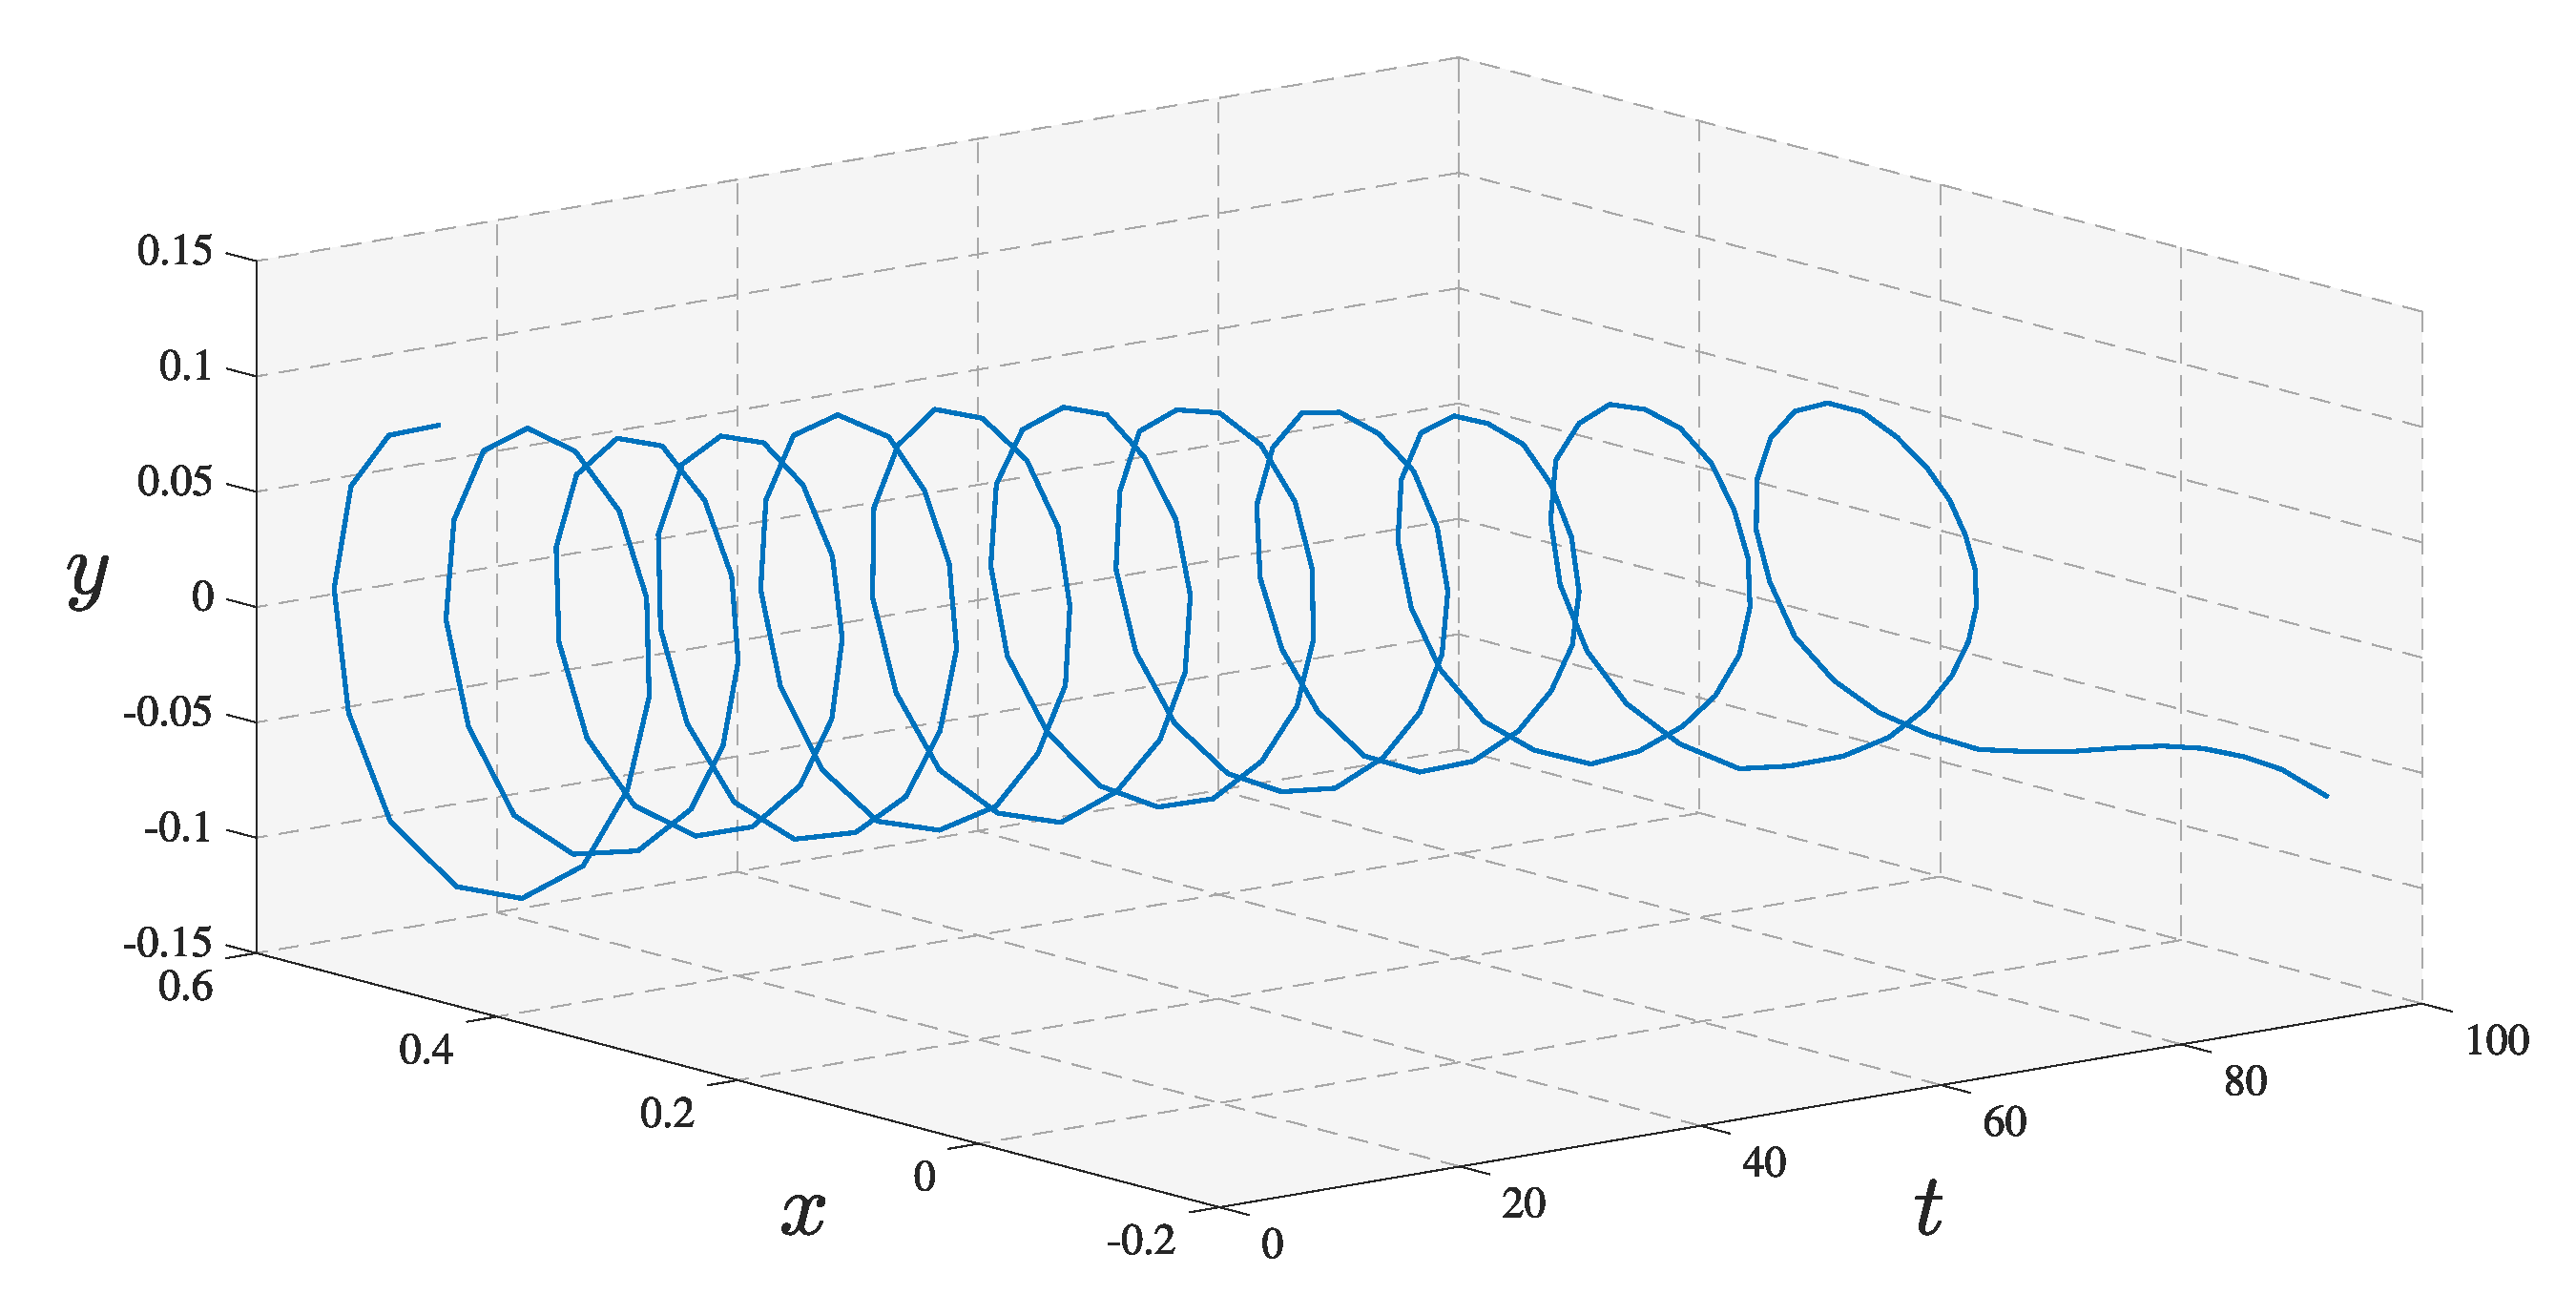
\includegraphics[width = 0.9\columnwidth]{Homoclinic3D}
	\caption{A single realisation of the system in equation~\ref{eqn:2D:homoclinicSystem} with initial point $(\sqrt{0.2},0.1)$. The system spirals around the moving centre at $(\sqrt{\alpha},0)$, $\alpha$ is given in equation~\ref{eqn:2D:homoclinicAlpha}, until $t=100$, $\alpha=0$, when the bifurcation occurs and the system tends towards infinity in the negative $x$ and negative $y$ directions.
		\label{fig:2D:Homoclinic3D}}
\end{figure}

We consider the system given by equations
	\begin{equation}
		\begin{array}{rcl}
		\dot{x} &=& y + \eta^{(x)},\\
		\dot{y} &=& \alpha - x^2 + \eta^{(y)},
		\end{array}
	\label{eqn:2D:homoclinicSystem}
	\end{equation}
where $\eta^{(x)}$, $\eta^{(y)}$ are white noise terms. If we ignore these noise terms, we find that the system has steady state solutions at $(x,y) = (\pm \sqrt{\alpha},0)$. The Jacobian of the system is given by 
	\begin{equation}
		J(x,y) = \left(\begin{array}{cc}
		0 & 1 \\ -2x & 0
		\end{array}\right)\,,
	\label{eqn:2D:homoclinicJacobian}
	\end{equation}
and has eigenvalues $\lambda = \pm \sqrt{-2x}$. The eigenvalues at the stable solutions are:
\begin{itemize}
	\item at $(-\sqrt{\alpha},0)$: $\lambda = \pm(4\alpha)^{1/4}$, indicating that this is a saddle,
	\item at $(+\sqrt{\alpha},0)$: $\lambda = \pm i(4\alpha)^{1/4}$, indicating that this is a stable centre.
\end{itemize}
\cite{williamson2015} allow $\alpha$ to vary and to approach zero from above. At $\alpha=0$ the two stable points collide resulting in a bifurcation and there are no stable solutions for $\alpha<0$. {\Red{ Before the bifurcation, the evolution of the system resembles a near-homoclinic orbit around the stable centre. This orbit becomes more and more pointed as the bifurcation approaches as the system spends more and more time close to the saddle point on each period. This looks like a system approaching a homoclinic bifurcation, in which the orbit eventually joins with the saddle and becomes homoclinic, and then disconnects from the saddle with further change in the system parameter (see equation~\ref{eqn:intro:trueHomoclinic}, page~\pageref{eqn:intro:trueHomoclinic} for an example of such a system). In this system, however, the orbit shrinks around the stable centre and, at the point of bifurcation, the centre meets with the saddle at the same time at which the orbit shrinks down to zero-radius, so the orbit does not actually become homoclinic. 
		
If we consider the system equations without the stochastic component, that is,
	\begin{equation}
	\begin{array}{rcl}
		\dot{x} &=& y ,\\
		\dot{y} &=& \alpha - x^2 ,
		\end{array}
		\label{eqn:2D:homoclinicSystem_deterministic}
	\end{equation}
we note this is equivalent to the second order differential equation
	\begin{equation}
		\ddot{x} = \alpha - x^2,
	\label{eqn:2D:homoclinicSystem_secondorder}
	\end{equation}
which has potential function
	\begin{equation}
		V(x) = \frac{x^3}{3} - \alpha x,
	\end{equation} 
since this results in
	\begin{equation}
		\ddot{x} = -\frac{\partial}{\partial x}V(x)\,.
	\end{equation} 
Since the energy 
	\begin{equation}
		E(x) = \frac{\dot{x}^2}{2}+V(x) = \frac{y^2}{2} + \frac{x^3}{3} - \alpha x\,,
	\end{equation} 
is a conserved quantity, that is, $\dot{E}(x)=0$, $E(x)=c$ for some constant $c$, then we have that the solutions to the ODE are given by
	\begin{equation}
		\frac{y^2}{2} + \frac{x^3}{3} - \alpha x =c\,.
		\label{eqn:2D:SystemA_solutions}
	\end{equation} 
This set of solutions is represented in figure~\ref{fig:2D:systemA_circles} where the solution is plotted for $10$ values of $c$ in the range $-1\leq c \leq 1$, with $\alpha=1$. We note the stable point at $x=\sqrt{\alpha}=1,~ y=0$ surrounded by concentric egg-shape `circles'. Thus, the system is not spiralling inwards toward the stable point, nor outwards. 
	}}

\begin{figure}
	\centering
	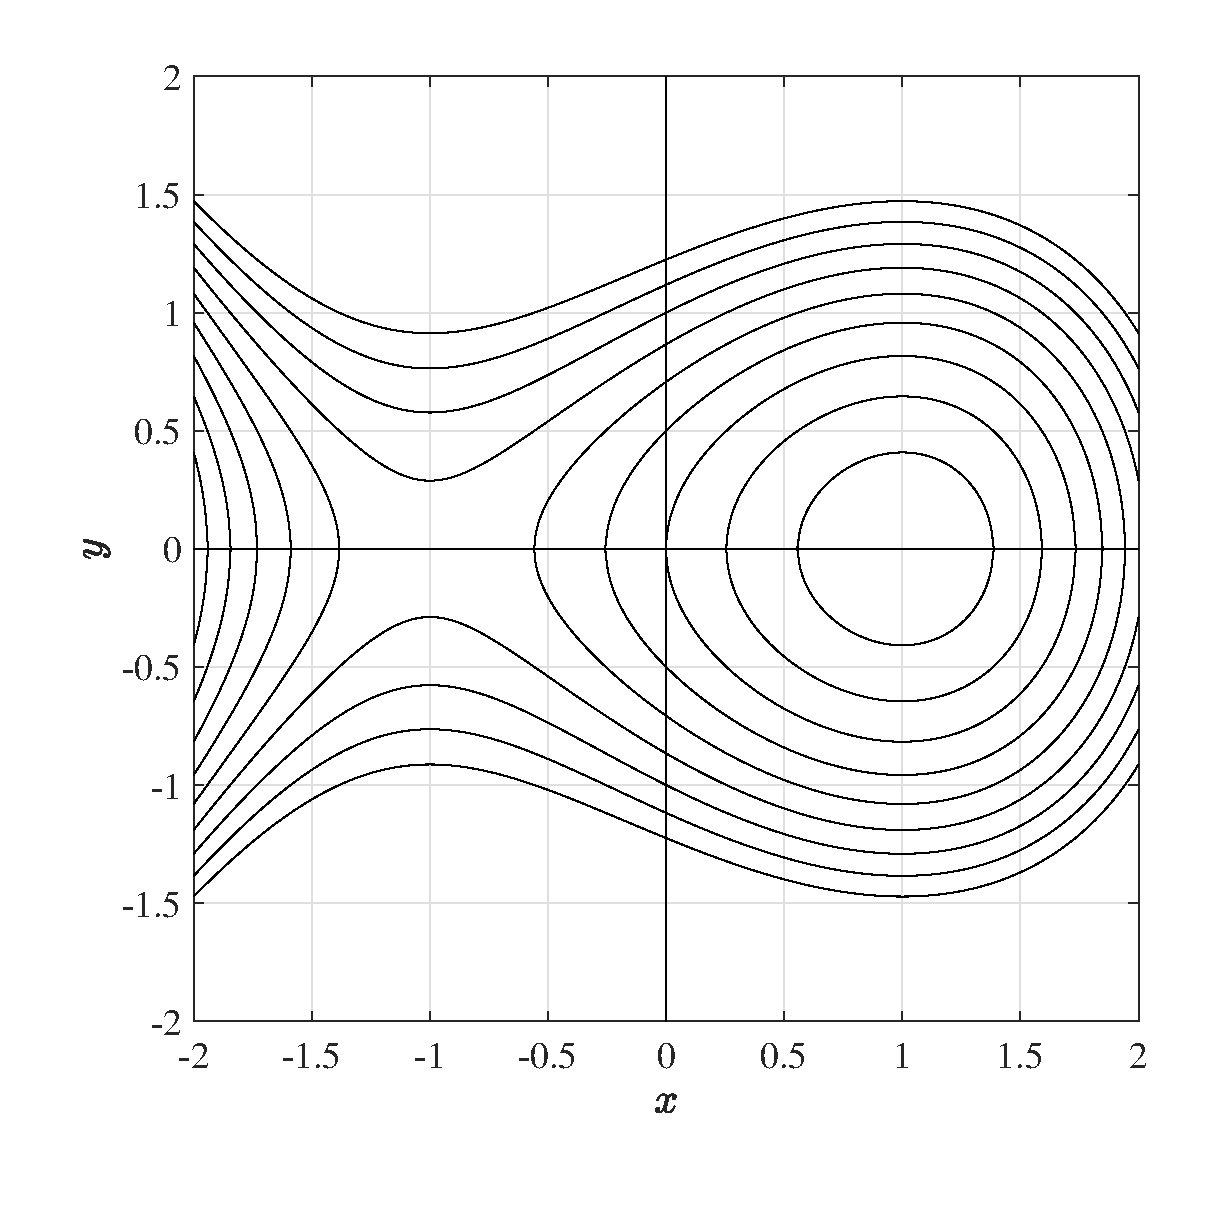
\includegraphics[width = 0.4\columnwidth]{systemA_circles}
	\caption{\Red{The solutions for System A (see equation~\ref{eqn:2D:SystemA_solutions}) are plotted for $\alpha=1$ with $10$ values of $c$ in the range $-1\leq c \leq 1$. A single stable point occurs at $(1,0)$ while a saddle exists at $(\m1, 0)$.
	}}
	\label{fig:2D:systemA_circles}
\end{figure}
%systemA_circles


\cite{williamson2015} consider a point at or close to the stable centre 
$(+\sqrt{\alpha},0)$, with noise terms $\eta^{(x)}$, $\eta^{(y)}$ in equation \ref{eqn:2D:homoclinicSystem} having standard deviation of 0.01. At this centre the eigenvalues of the Jacobian have zero real part but imaginary part of $\pm(4\alpha)^{1/4}$. If we take the eigenvalue with positive imaginary part we expect to see it decrease as $\alpha$ decreases to zero. This is the early warning signal of the bifurcation. 

We integrate the system in equations \ref{eqn:2D:homoclinicSystem} from $t=0$ to $t=100$, using a varying parameter
	\begin{equation}
		\alpha(t) = 0.2 - 0.002t,
	\label{eqn:2D:homoclinicAlpha}
	\end{equation}
so that the bifurcation when $\alpha = 0$ will occur at $t=100$. Noise terms $\eta^{(x)}$, $\eta^{(y)}$ are independent with zero mean and standard deviation 0.01 and the solution is sampled at intervals of $\Delta t = 0.5$. The result of one such integration is plotted in figure~\ref{fig:2D:Homoclinic3D}.

\begin{figure}
	\centering
	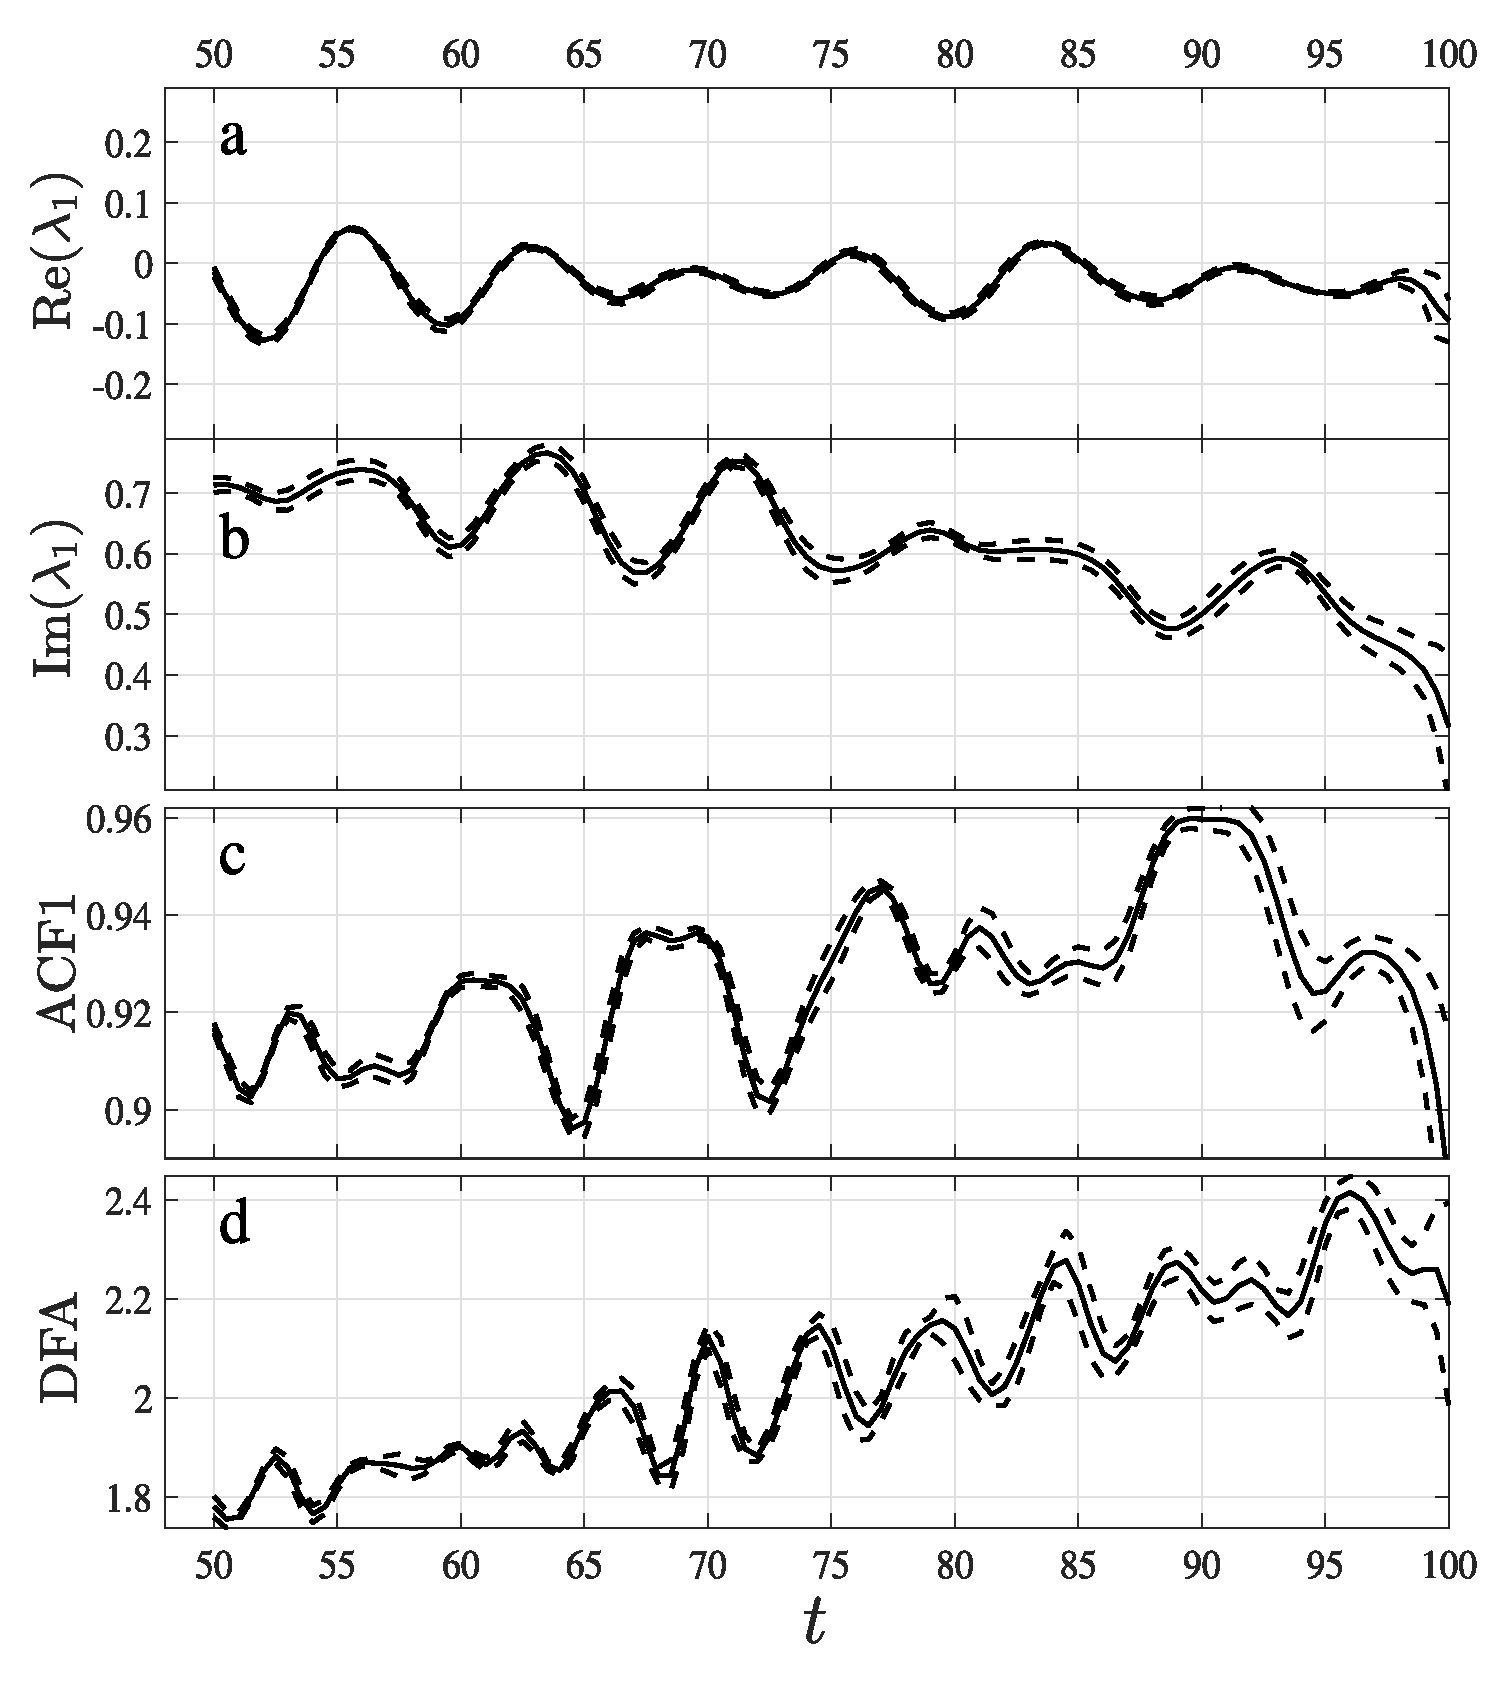
\includegraphics[width = 0.9\columnwidth]{HomoclinicIndicators}
	\caption{Tipping point indicators applied to System A (equation~\ref{eqn:2D:homoclinicSystem}) which experiences a bifurcation at $t=100$. Panels \textbf{a} and \textbf{b} show the real and imaginary parts of the first reconstructed eigenvalue of the Jacobian matrix, as in equation~\ref{eqn:2D:williamson-eigenvalueRelations}. Panels \textbf{c} and \textbf{d} show the ACF1 and DFA indicators calculated with a window size of 100 points, applied to the one-dimensional time series obtained by applying EOF dimension reduction to the data. The system was integrated ten times and the mean over ten data sets is plotted, along with error of one standard deviation (dashed lines).
	\label{fig:2D:HomoclinicIndicators}}
\end{figure}

We now attempt to provide an early warning signal of the impending bifurcation. The autocorrelation matrix $A$ is calculated using equation \ref{eqn:2D:williamson-AR1analogue} in a sliding window of 100 points. The Jacobian eigenvalues are recovered using equations \ref{eqn:2D:williamson-eigenvalueRelations} and the real and imaginary parts of the first eigenvalue (the eigenvalue with positive imaginary part) are calculated. This procedure is applied to ten realisations of the system, and the mean is shown in figure~\ref{fig:2D:HomoclinicIndicators}a,b with error bars of one standard deviation. The figure shows a successful reproduction of the results of \citet{williamson2015}: the real part of the eigenvalue is $\approx 0$ with little variability, as expected for $\mu>0$, and the decreasing imaginary part of the eigenvalue predicates the bifurcation as $\alpha\rightarrow0$, as predicted by the analysis. 

As a comparison, the ACF1 and DFA indicators are applied to the same data using a 100 point window size and after reducing the dimension of the system using EOFs. The results are shown in figure~\ref{fig:2D:HomoclinicIndicators}c,d. Both indicators show a general upwards trend prior to the bifurcation at $t=100$, but the ACF1 indicator contains more variability. 



\subsubsection{System experiencing a Hopf bifurcation (System B)}
\label{subsec:2D:MethodsApplied:WilliamsonHopf}

\begin{figure}
	\centering
	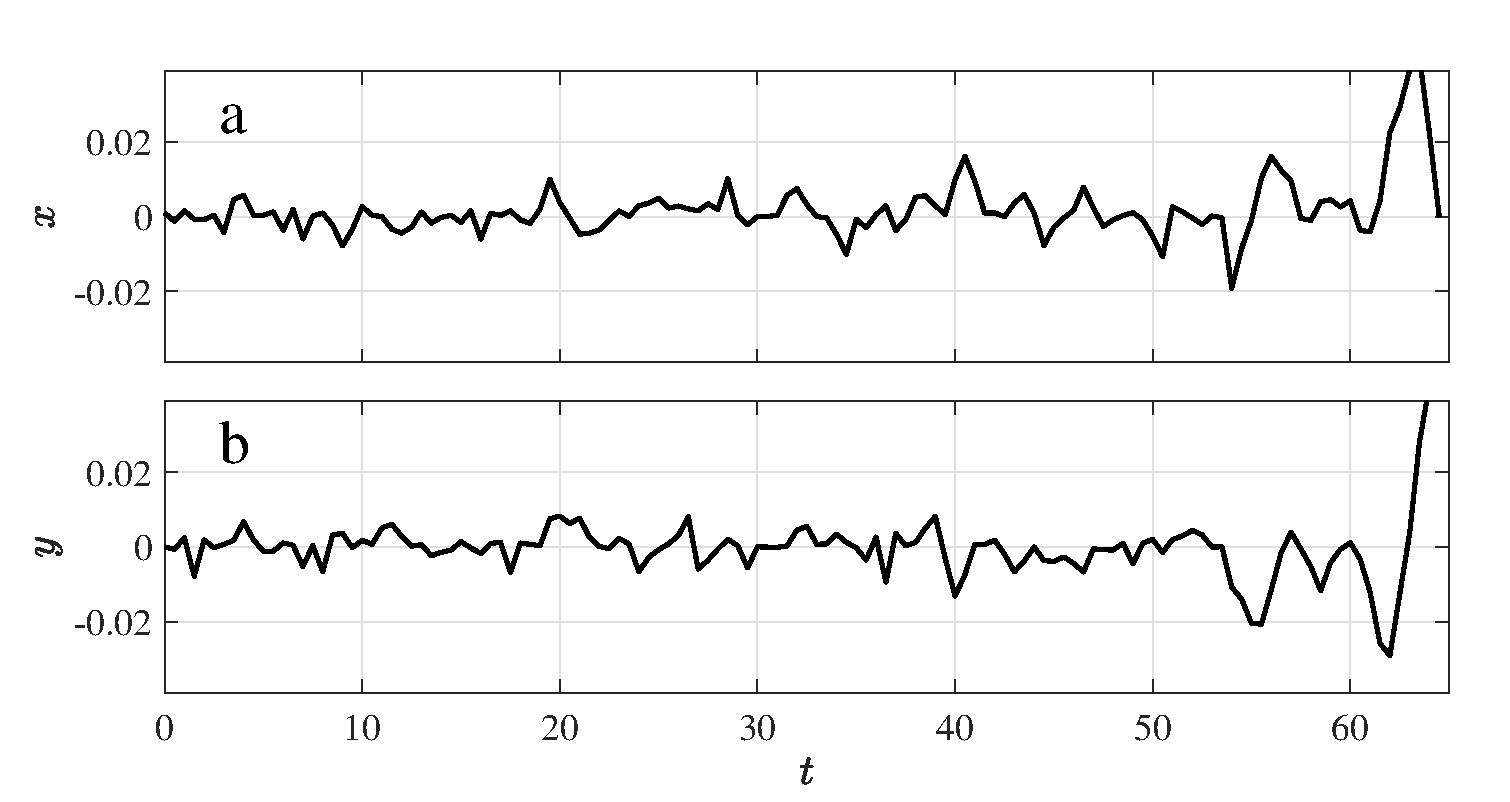
\includegraphics[width = 0.9\columnwidth]{HopfIllustration_EM}
	\caption{A single realisation of the system in equation~\ref{eqn:2D:HopfSystem_noise} with initial point $(0,0)$. The system oscillates about the stable point $(0,0)$ until $t=58$ when the bifurcation occurs and the stability is lost.
		\label{fig:2D:HopfIllustration}}
\end{figure}

We now consider the second example given by \citet{williamson2015}, the system given by the polar equations 
	\begin{equation}
		\begin{array}{rcl}
			\dot{r} &=& \mu r - r^3,\\
			\dot{\theta} &=& 1 + r^2.
		\end{array}
		\label{eqn:2D:HopfSystem}
	\end{equation}
The system is a classic example of a supercritical Hopf bifurcation. The normal form of the Hopf bifurcation is
\begin{equation}
	\dot{z} = z\left((\lambda+i)+b|z|^2\right),
\end{equation}
where $z$ and $b=\alpha+i\beta$ are complex numbers. 
If we rewrite the system in equation \ref{eqn:2D:HopfSystem} according to $z = \exp(i\theta)$, we get
	\begin{align}
		\begin{split}
			\dot{z} &= \dot{r}e^{i\theta}+ir\dot{\theta}e^{i\theta}\\
			&= re^{i\theta}\left(\frac{\dot{r}}{r}+i\dot{\theta}\right)\\
			&= re^{i\theta}\left((\mu-r^2)+i(1+r^2)\right)\\
			&= z\left((\mu+i)+(i-1)|z|^2\right).
		\end{split}
	\end{align}

The system has stable solution at $r=0$ for $\mu<0$. At $\mu=0$ a bifurcation occurs and $r=0$ becomes unstable, whilst two stable solutions for $r$ are created at $r = \pm\sqrt{\mu}$. Since $\theta$ increases at a constant rate $\dot{\theta}=1+\mu$, or almost constant if an additional noise term is introduced into equation~\ref{eqn:2D:HopfSystem}, this results in a stable limit cycle with radius $r=\sqrt{\mu}$. 

We may also investigate the nature of the bifurcation by studying the eigenvalues of the Jacobian of the system equations. In Cartesian rather than polar coordinates we have
	\begin{equation}
		J(x,y) =  
		\left(
		\begin{array}{cc}
		\mu - (x+y)^2-2x^2 & -1-(x+y)^2-2y^2\\
		1+(x-y)^2 + 2x^2 & \mu - (x-y)^2-2y^2
		\end{array} \right).
	\label{eqn:2D:HopfJacobian}
	\end{equation}
At the stable point $r=0$ (i.e. $(x,y)=(0,0)$), the matrix $J(x,y)$ has complex conjugate eigenvalues $\lambda=\mu\pm i$. The system therefore experiences a Hopf bifurcation as $\mu$ approaches zero from below, characterised by the Jacobian eigenvalues moving from the negative-real to the positive-real half of the complex plane.

We reproduce the numerical results of \citet{williamson2015} using a varying parameter
	\begin{equation}
		\mu(t) = 0.05t - 2.9\,,
	\label{eqn:2D:HopfParameter}
	\end{equation} 
and integrate the system from $t=0$ to $t=60$ with the solution given at intervals $\Delta t = 0.2$. The bifurcation at $\mu = 0$ will occur at $t=58$. Gaussian noise terms $\eta^{(r)}$ and $\eta^{(\theta)}$ are also added to the system equations for $r$ and $\theta$ respectively:
	\begin{equation}
		\begin{array}{rcl}
		\dot{r} &=& \mu r - r^3 + \eta_r\,,\\
		\dot{\theta} &=& 1 + r^2 + \eta_\theta\,,
		\end{array}
	\label{eqn:2D:HopfSystem_noise}
	\end{equation}
where $\eta_r$, $\eta_\theta$ both have zero mean and standard deviation $0.01$. The result is shown in figure~\ref{fig:2D:HopfIllustration}. 

\begin{figure}
	\centering
	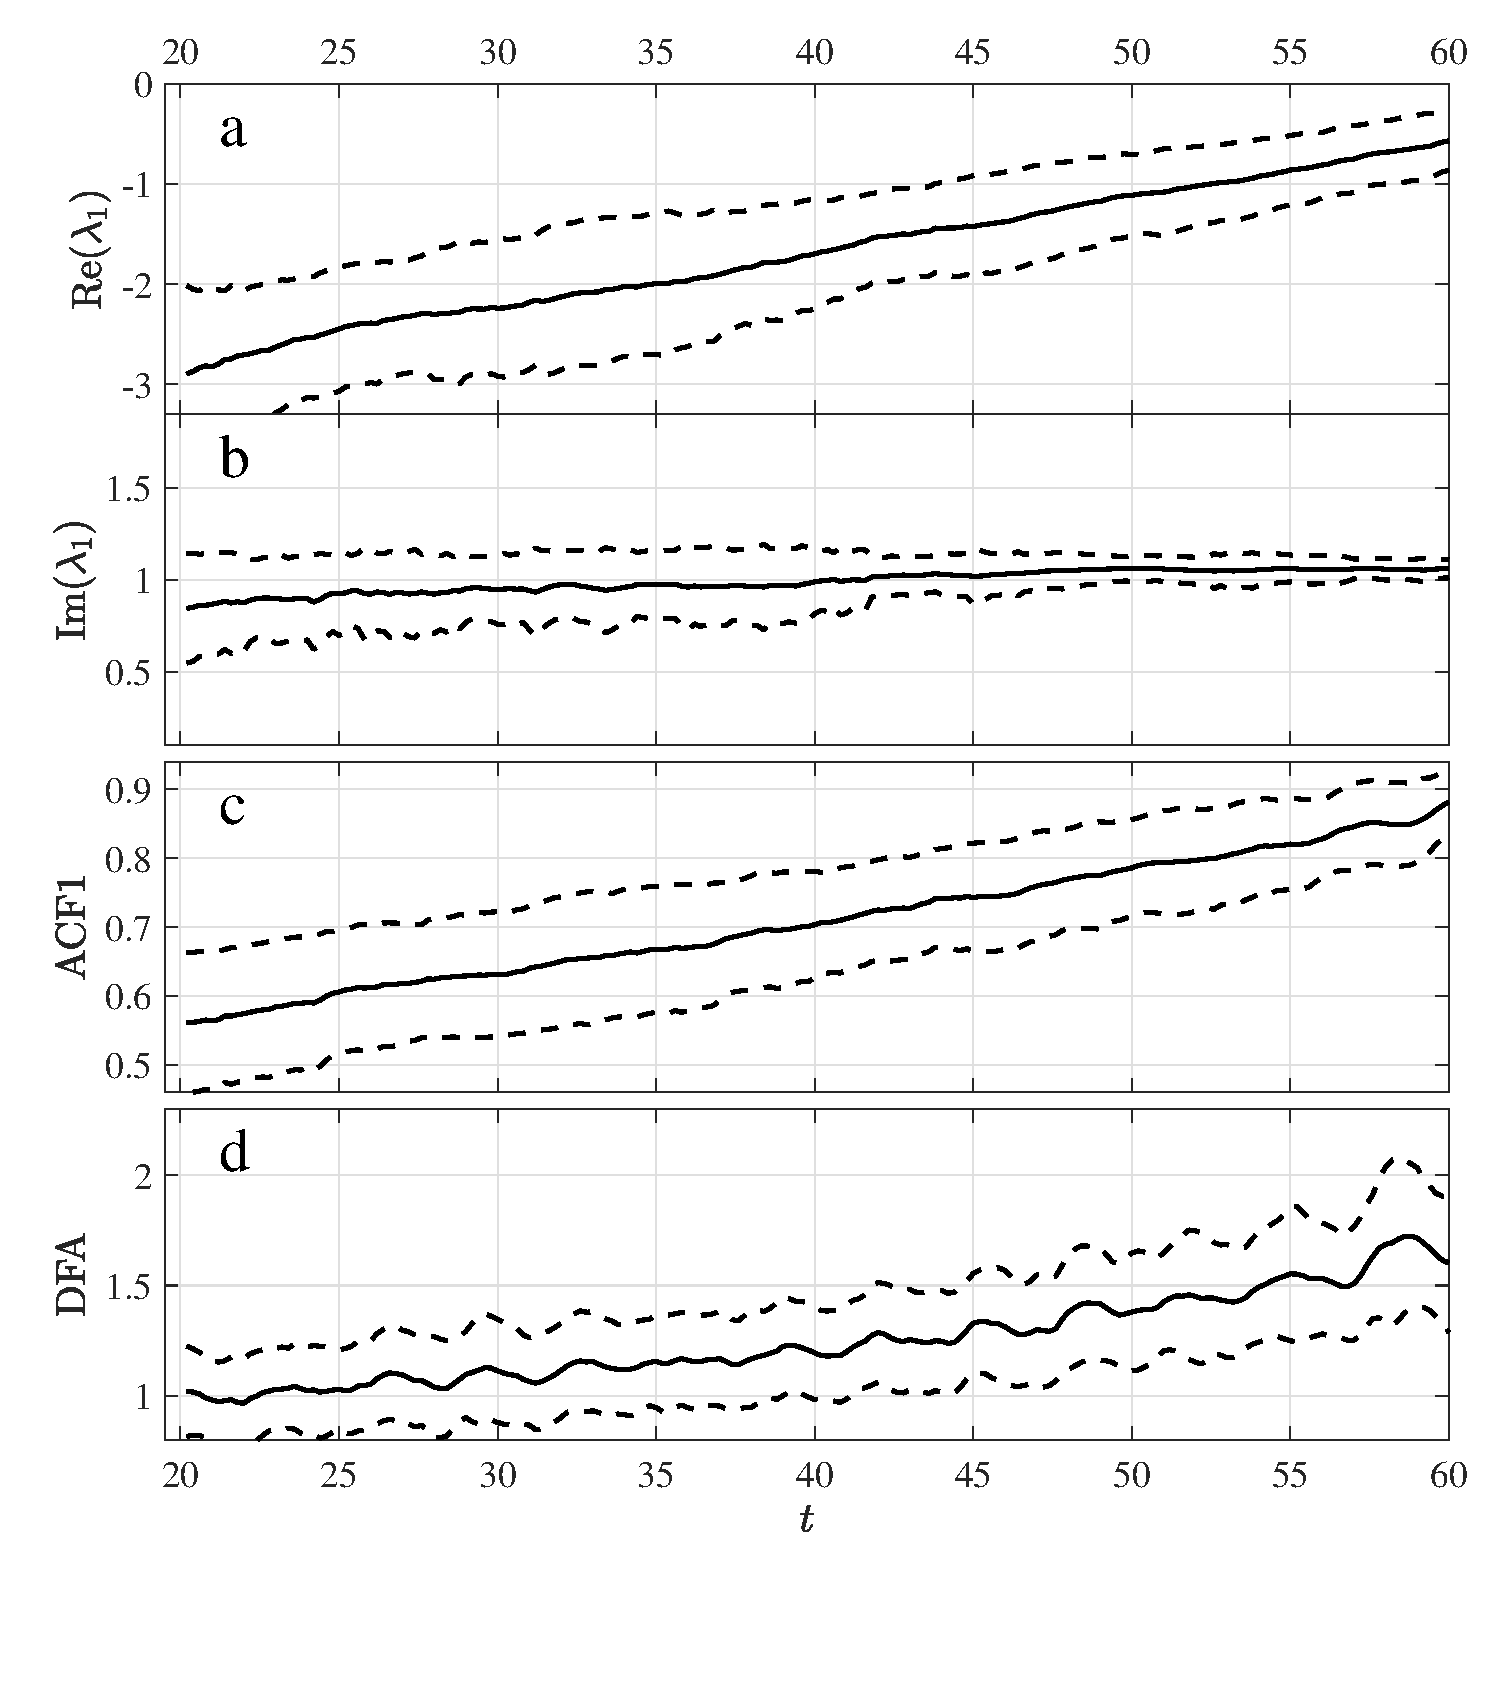
\includegraphics[width = 0.9\columnwidth]{HopfIndicators_EM}
	\caption{Tipping point indicators applied to System B (equation~\ref{eqn:2D:HopfSystem_noise}) which experiences a Hopf bifurcation at $t=58$. Panels \textbf{a} and \textbf{b} show the real and imaginary parts of the first reconstructed eigenvalue of the Jacobian matrix, as in equation~\ref{eqn:2D:williamson-eigenvalueRelations}. Panels \textbf{c} and \textbf{d} show the ACF1 and DFA indicators calculated with a window size of 100 points, applied to the one-dimensional time series obtained by applying EOF dimension reduction to the data. The system was integrated $100$ times and the mean over the $100$ data sets is plotted, along with error of one standard deviation (dashed lines).
		\label{fig:2D:HopfIndicators}}
\end{figure}

As in the previous example, the autocorrelation matrix $A$ is calculated using equation~\ref{eqn:2D:williamson-AR1analogue} in a sliding window of 100 points. The Jacobian eigenvalues are recovered using equation~\ref{eqn:2D:williamson-eigenvalueRelations} and the real and imaginary parts of the first eigenvalue are plotted in figure~\ref{fig:2D:HopfIndicators}a,b.

In this example, as in the previous, we are able to successfully reproduce the results of \citet{williamson2015}.


\subsubsection{The Van der Pol oscillator (System C)}
\label{subsec:2D:MethodsApplied:WilliamsonVanDerPol}
\begin{figure}
	\centering
	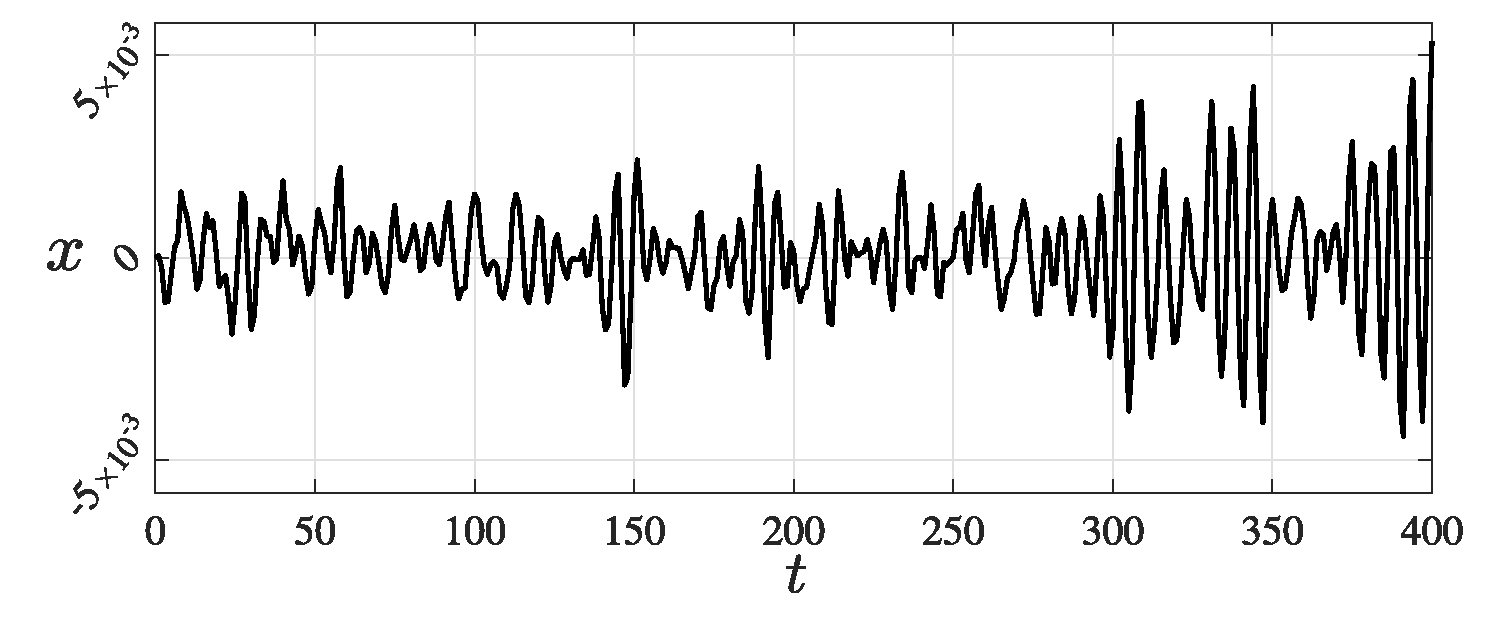
\includegraphics[width = 0.9\columnwidth]{vdpIllustration}
	\caption{A single realisation of the Van der Pol system in equation~\ref{eqn:2D:VDPSystemCoupled} with initial point $(0,0)$. The system oscillates about the centre at $(0,0)$ until $t=380$, $\mu=0$, when the Hopf bifurcation occurs and stability is lost.
		\label{fig:2D:vdpIllustration}}
\end{figure}

Here, we consider another example of a Hopf bifurcation, allowing us to apply the method introduced by \citet{williamson2015} to a novel system. We consider the Van der Pol oscillator \citep{vanDerPol1926} given by
	\begin{equation}
		\ddot{x} - \mu(1-x^2)\dot{x} + x = \eta,
		\label{eqn:2D:VDPSystem}
	\end{equation}
where the stochastic forcing term $\eta$ is white noise with standard deviation 0.01. We may also write equation \ref{eqn:2D:VDPSystem} as a coupled system of first order ODEs:
	\begin{equation}
		\begin{array}{rcl}
		\dot{x} &=& \mu\left(x - \frac{1}{3}x^3\right)+y,\\
		\dot{y} &=& -x + \eta.
		\end{array}
		\label{eqn:2D:VDPSystemCoupled}
	\end{equation}
The system has a stable equilibrium point ($\dot{x}= \dot{y}= 0$) at $(x,y)= (0,0)$ for $\mu<0$ which becomes the centre of a stable limit cycle for $\mu>0$. The Jacobian of this system is calculated:
	\begin{equation}
		J(x,y) = \left(
		\begin{array}{cc}
		\mu(1-x^2) & 1\\
		-1 & 0
		\end{array}
		\right).
		\label{eqn:2D:VDPJacobian}
	\end{equation}
Evaluated at the stable point $(0,0)$, the two complex-conjugate eigenvalues of the Jacobian are $\lambda = \frac{1}{2}(\mu \pm \sqrt{\mu^2-4})$. We therefore expect that the real part of both of the eigenvalues, equal to $\mu/2$, will approach zero as $\mu$ approaches zero from below, i.e. as the system approaches the bifurcation. 

We integrate the system in equations \ref{eqn:2D:VDPSystemCoupled} from $t=0$ to $t=400$ using a time dependent parameter
	\begin{equation}
		\mu(t) = -0.38 + 0.001t,
		\label{eqn:2D:vdpParameter}
	\end{equation} 
so that the bifurcation $\mu=0$ will occur at $t=380$. Using the method described, we estimate the first eigenvalue of the Jacobian in a sliding window of 100 points. The mean (with error bars of one standard deviation) of 10 such experiments is shown in figure~\ref{fig:2D:vdpIndicators}. We note that the real part of the eigenvalue increases as expected and provides an early warning signal of the impending Hopf bifurcation.

\begin{figure}
	\centering
	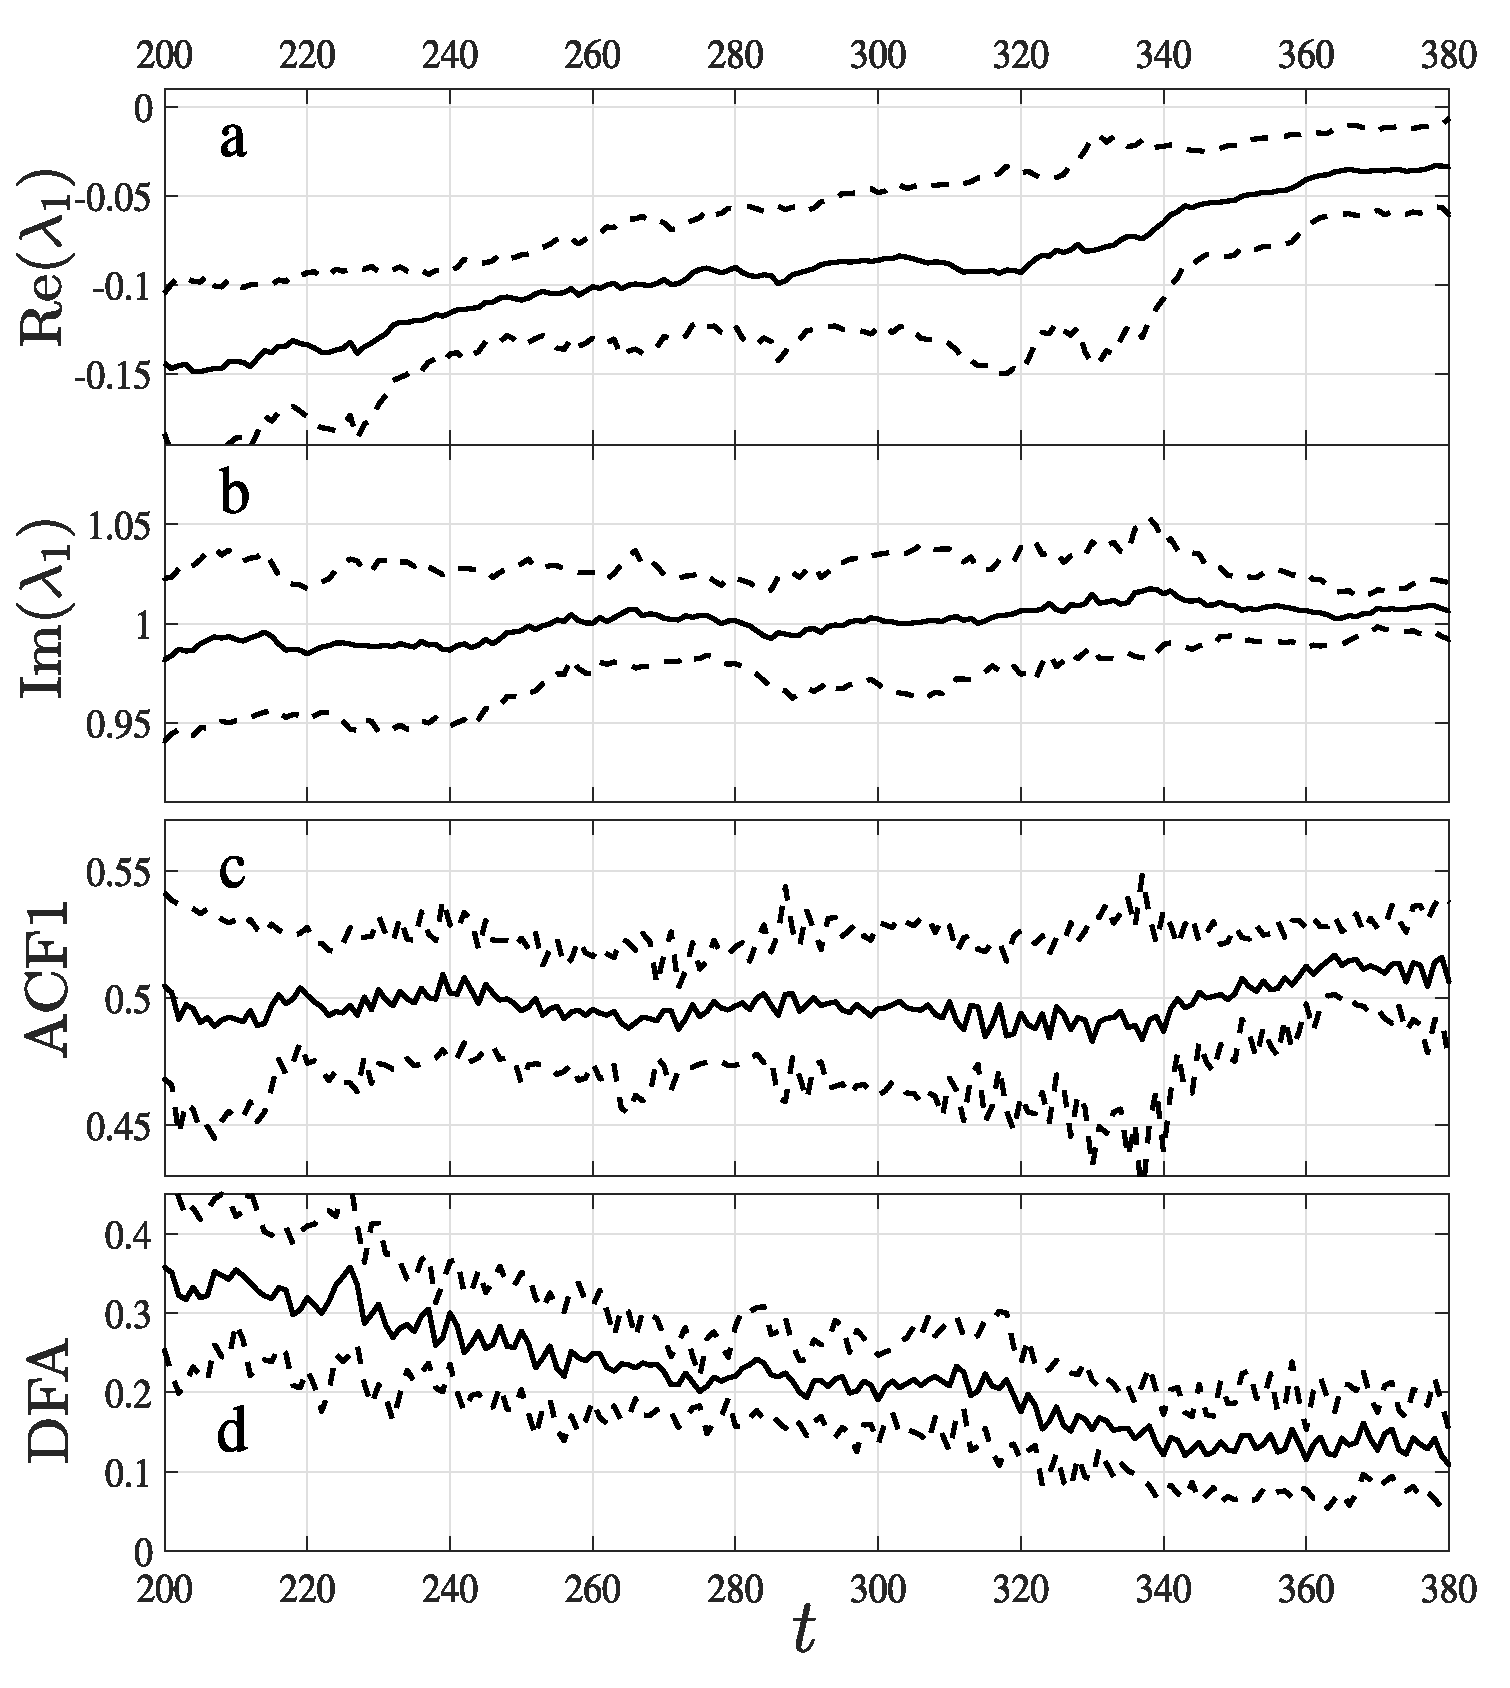
\includegraphics[width = 0.9\columnwidth]{VdpIndicators}
	\caption{Tipping point indicators applied to System C, the Van de Pol oscillator (equation~\ref{eqn:2D:VDPSystemCoupled}), which experiences a Hopf bifurcation at $t=380$. Panels \textbf{a} and \textbf{b} show the real and imaginary parts of the first reconstructed eigenvalue of the Jacobian matrix, as in equation~\ref{eqn:2D:williamson-eigenvalueRelations}. Panels \textbf{c} and \textbf{d} show the ACF1 and DFA indicators calculated with a window size of 100 points, applied to the one-dimensional time series obtained by applying EOF dimension reduction to the data. The system was integrated ten times and the mean over ten data sets is plotted, along with error of one standard deviation (dashed lines).
		\label{fig:2D:vdpIndicators}}
\end{figure}

\subsection{Application of the novel PS indicator}
\label{subsec:2D:MethodsApplied:PS-indicator}

We also calculate the PS indicator in the three systems described in this section, in addition to the ACF1 and DFA indicators and the Jacobian eigenvalues as shown in figures~\ref{fig:2D:HomoclinicIndicators}-\ref{fig:2D:vdpIndicators}. Systems A, B and C (see equations~\ref{eqn:2D:homoclinicSystem}, \ref{eqn:2D:HopfSystem_noise} and \ref{eqn:2D:VDPSystemCoupled}) are integrated and the PS indicator is calculated, in all three cases, using a sliding window of 100 points, similarly to the other indicator methods. This is done ten times for each system and the mean of the PS indicator is found, as shown in figure~\ref{fig:2D:PS-indicators}. We see that the PS indicator does not provide an EWS for the bifurcation in systems A and C, and the signal is very weak, obscured by its variability, in system B. In all three cases the DFA indicator, as presented in figures~\ref{fig:2D:HomoclinicIndicators}-\ref{fig:2D:vdpIndicators}, provides a clearer EWS. 

\begin{figure}
	\centering
	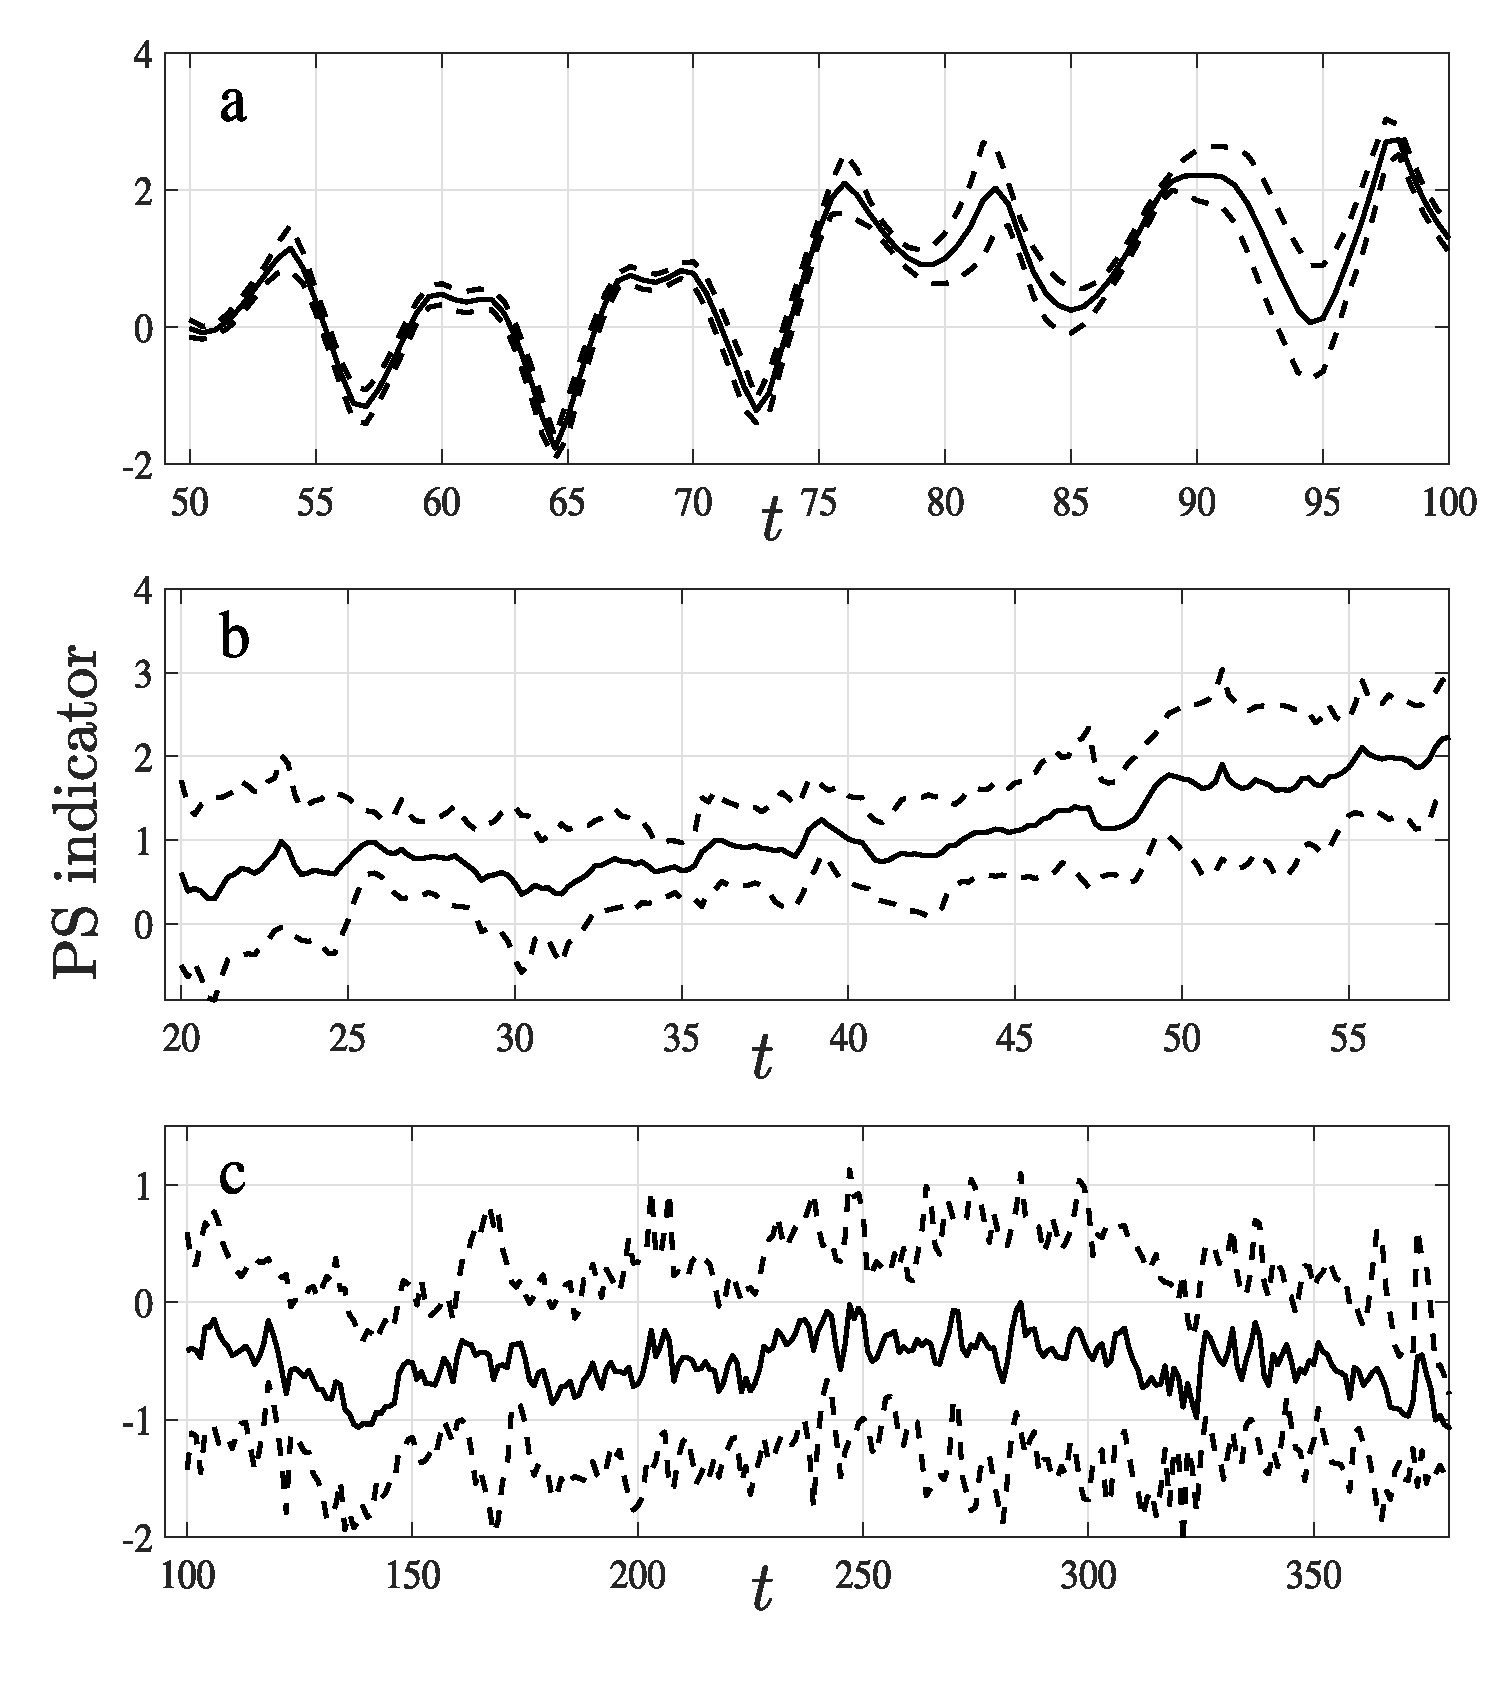
\includegraphics[width = 0.9\columnwidth]{PSindicators}
	\caption{PS indicator applied to the three systems described in this section after reducing each system to one dimension using the EOF method. The results for systems A, B and C are shown in panels \textbf{a}, \textbf{b} and \textbf{c} respectively. In each plot the bifurcation occurs at the last point on the $t$-axis: $t=100$, $t=58$ and $t=380$ respectively. Each system was integrated ten times and the mean over ten data sets is plotted, along with error of one standard deviation (dashed lines).
		\label{fig:2D:PS-indicators}}
\end{figure}



\subsection[Investigation of updated EOF projection]{Investigation of updated EOF projection with the ACF1 indicator}
\label{subsec:2D:MethodsApplied:Hopf_movingEOF}

In section~\ref{subsec:2D:EOF:movingEOF} it is remarked that in a practical prediction problem one cannot obtain a single EOF score with which to calculate a tipping point indicator. More sensibly, the EOF eigenvector, onto which the multi-variable time series is projected, would be updated at each iteration of the indicator calculation. Here we once again apply the ACF1 indicator to system B (see figure~\ref{fig:2D:HopfIndicators}b) but present the other available options. Figure~\ref{fig:2D:Hopf_movingEOF} shows the result of using the global EOF projection (as in figure~\ref{fig:2D:HopfIndicators}b) alongside the windowed EOF projection, in which only the current window of data is considered, and the moving EOF projection, in which the EOF eigenvector is updated using new data as time progresses without disregarding any previous data.
\begin{figure}
	\centering
	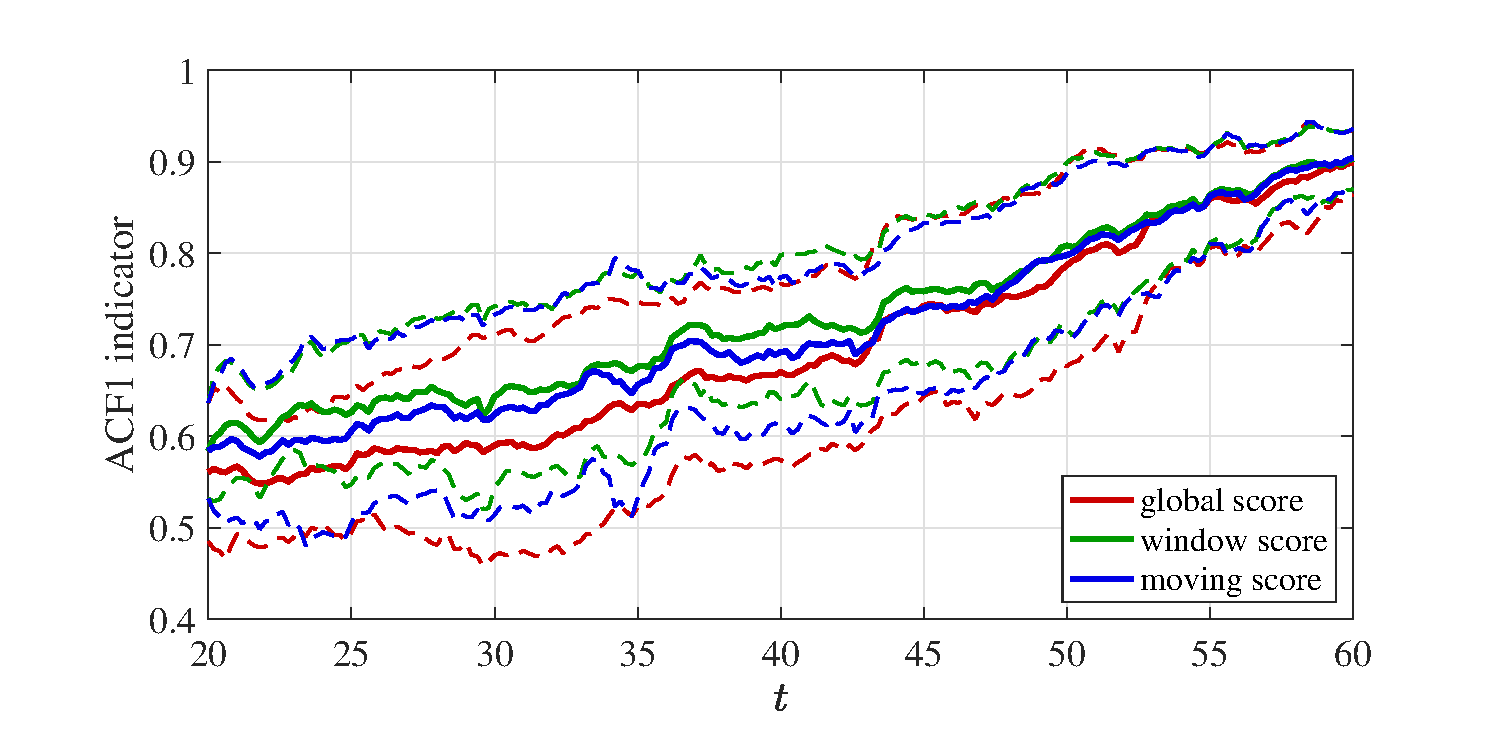
\includegraphics[width = 0.9\columnwidth]{HopfEOF}
	\caption{ACF1 indicator applied to System B in conjunction with EOF dimension reduction. Three different options for the EOF calculation are used: the global, windowed and moving EOF projections (red, blue and green respectively). For each of the three options, the system was integrated ten times and the mean over ten data sets is plotted, along with error of one standard deviation (dashed lines).
		\label{fig:2D:Hopf_movingEOF}}
\end{figure}

We note that the three options do not differ significantly. In particular, the fact that the global and windowed approaches yield very similar results demonstrates that the principal EOF eigenvector does not change significantly over time. In systems where the EOF eigenvector is likely to change over time, it would be best to use the windowed projection approach for practical problems so that the optimal variance-maximising projection is always used. However, this may introduce noise-induced error, particularly when the window size is short. 

\subsection{Discussion of results}
\label{subsec:2D:MethodsApplied:discussion}
{\Red{
In this section we have calculated the ACF1, DFA and PS indicators for three different dynamical systems in order to provide an early warning signal. Unlike in chapter~\ref{chap:1D} (see section~\ref{sec:1D:indicatorComparison}) we did not have a one-dimensional time series to which these methods might be applied, the EOF projections of the two-dimensional time series were therefore used. In addition we have obtained an additional early warning signal, from the `eigenvalue indicator', using the method of \cite{williamson2015} (see section~\ref{sec:2D:Williamson}). 

In the cases of Systems A and B the results of \cite{williamson2015} are faithfully reproduced. The imaginary part of the first eigenvalue decreases as an EWS of the bifurcation in System A, and the real part of the first eigenvalue increases as an EWS of the Hopf bifurcation in System B. When applied to System C, the Van der Pol oscillator, the real part of the first eigenvalue increases, which is to be expected since the tipping point in this case is also a Hopf bifurcation. We therefore verify the method in a new system, where the same indicator predicts the same variety of bifurcation (Hopf). 

The one-dimensional EWS methods introduced in chapter~\ref{chap:1D} were applied to the EOF projection of the time series in each case. We find that for Systems A and B these methods do provide an EWS in the sense that the indicators increase prior to the tipping point. That is, the indicators are higher in each case when the system parameter is closer to the critical value. This increase is clearer in the ACF1 and DFA indicators than in the PS indicator, and we note that the PS indicator also showed the least significant increase in all the one-dimensional systems studied in chapter~\ref{chap:1D}, so this is not surprising. In the case of System A, all three indicators suffer from large fluctuations which disguise any increase due to the presence of the tipping point itself. These fluctuations are likely due to the oscillations in System A, which orbits around the stable centre until it crosses the saddle node and diverges. This oscillation will be investigated further, and solutions proposed, in section~\ref{sec:2D:periodic_orbit}. 

In the case of System C, the Van der Pol oscillator, none of these three indicators provided an EWS. The ACF1 and PS indicators remained approximately constant as the bifurcation approached, whilst the DFA indicator apparently \emph{decreased} significantly. In this case the eigenvalue indicator performed much better than the combination of the EOF projection and the one-dimensional indicators. The problem may lie, again, with the oscillations in the system. 

}}


\section{Dealing with periodicity in an orbiting system}
\label{sec:2D:periodic_orbit}
{\Red{

The poor performance of the early warning indicators, and the DFA indicator in particular, when applied to System A (equation~\ref{eqn:2D:homoclinicSystem}), may be in part attributable to the periodicity in the system since the methods are not designed with this aspect in mind \citep{williamson2016}. The data may appear highly correlated even far from the bifurcation due to the fact that the system is following an orbit, although each orbit is in fact simply a noisy variation of the last. The DFA method removes trends only by subtracting a quadratic or cubic fit to the data and will not necessarily eliminate the correlation due to an orbit, particularly if more than one periods of the orbit occur within a single DFA window. 

In this section we investigate the effect of the presence of the orbit on the performance of the early warning indicators and attempt to improve performance by replacing the time series with its Poincaré map. As an example we again use System A:
\begin{equation}
	\begin{array}{rcl}
	\dot{x} &=& y + \eta^{(x)},\\
	\dot{y} &=& \alpha - x^2 + \eta^{(y)},
	\end{array}
	\label{eqn:2D:homoclinicSystem_again}
\end{equation}
(reprinting of equation~\ref{eqn:2D:homoclinicSystem}) where $\eta^{(x)}$ and $\eta^{(y)}$ are Gaussian white noise terms and $\alpha$ is a parameter affecting the nature of the stable states. For $\alpha>0$ the system has a stable centre at $(x,y) = (\sqrt{\alpha}, 0)$ and a saddle point at $(\m\sqrt{\alpha},0)$, at $\alpha=0$ the two points meet and there are no stable solutions for $\alpha<0$. If the system is initially close to the stable centre $(\sqrt{\alpha}, 0)$ it will orbit around this point, eventually either converging towards the centre or spiralling outwards until it leaves the orbit and diverges to infinity once it reaches the saddle node. Experimentally we find that for $\alpha=1$ the system diverges if the initial radius (with $(\sqrt{\alpha}, 0)$ as the centre) is greater than $\approx 0.24$. As $\alpha$ decreases toward zero this limiting radius also decreases so than an initially convergent system becomes divergent close to the bifurcation. 
}}
\begin{figure}
	\centering
	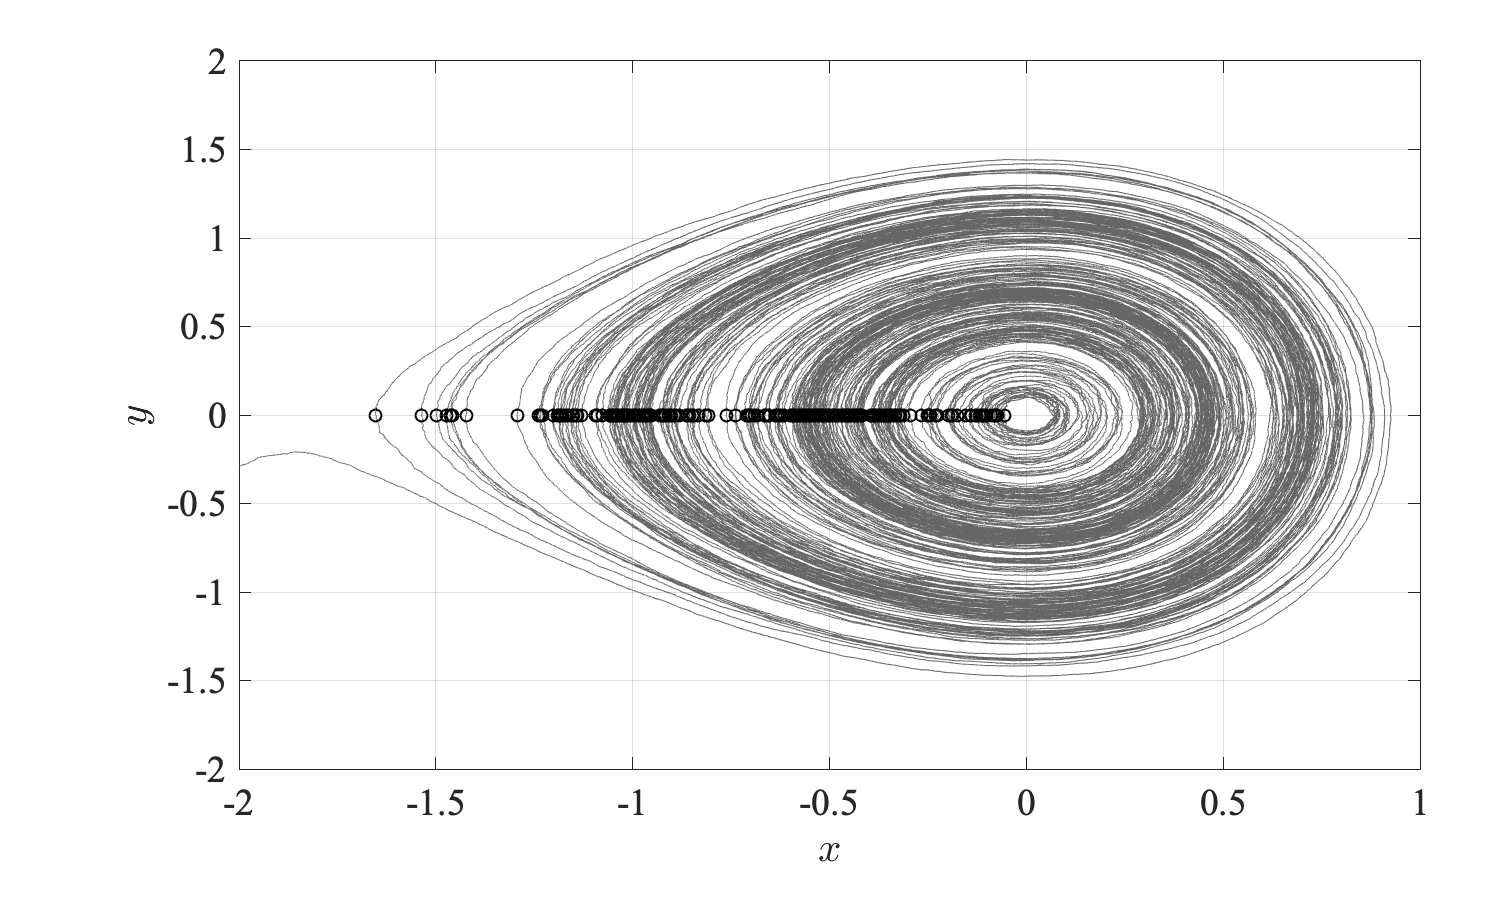
\includegraphics[width = 0.6\columnwidth]{periodicity_IntegrationPlusReturnPoints}
	\caption{\Red{ System A is integrated numerically with 
			$\Delta t = 0.01$ and $\alpha(t) = 1-10^{\m4}t$. The Poincar\'{e} return points for each orbit are also plotted (black circles).}}
	\label{fig:2D:periodicity:integration}
\end{figure}


\subsection{Methods}
\label{subsec:2D:periodic_orbit:methods}
{\Red{
In the original study of System A (see figure~\ref{fig:2D:HomoclinicIndicators}, page~\pageref{fig:2D:HomoclinicIndicators}) the periodicity was ignored and the early warning signals calculated using the raw data as an output of the numerical integration of the system equations. Here we present two alternative approaches to dealing with the periodicity.

\subsubsection{An approach based on the Poincaré map}

For a deterministic system $z(t)$ which orbits about a central point, the Poincaré map (see \cite{strogatz2014}) of a point $z(t_0)$ is the point $z(t_0+\tau) = P(z(t_0))$ such that the system has completed one periodic orbit during the time $\tau$. If $P(z(t_0)) = z(t_0)$ then the system has returned to exactly the same point after one period and therefore, if the system is deterministic, will continually repeat the same trajectory. 

In order to obtain a time series without oscillating behaviour, we consider the series of iterated Poincaré maps $z_n = P(z_{n-1})$ staring with an initial point $z_0$. In the case of System A (equation~\ref{eqn:2D:homoclinicSystem_again}) we take $z_0$ to be the first point on the half line $y=0,~x<\sqrt{\alpha}$, so that the series $[z_n]$ is the series of all the points which cross this half line as the system orbits around the point $(\sqrt{\alpha},0)$. We record only the $x$ coordinates since $y=0$ always, giving a one-dimensional time series.

\subsubsection{A periodic smoothing approach}

A potential drawback of the above Poincaré map method is that it reduces the length of the original time series by recording only one point per orbit. Alternatively, we may adopt a smoothing approach by taking the moving-mean of the data in a sliding window the length of which is the period of the orbit. 

In practice, for a two-dimensional time series in $x$ and $y$, we translate into polar coordinates $(r, \theta)$ centred on the sable point $(x_1, y_1)$ about which the system orbits. That is,
\begin{equation}
	\begin{array}{rcl}
	 	x &=& x_1 + r \cos(\theta)\,,\\
	 	y &=& x_2 + r \sin(\theta)\,.
	\end{array}
\end{equation}
Then from the original time series $(r(t), \theta(t))$ we have the new series $(\bar{r}(t), \theta(t))$ where 
\begin{equation}
 	\bar{r}(t_k) = \frac{1}{n}\sum_{t = t_{k-n+1}}^{t_k}r(t)\,,
\end{equation} 
and $n$ is the smallest integer $>0$ such that $\theta(t_k) = \theta(t_{k-n})$. That is, $t_k - t_{k-n}$ is the period of the orbit. We note that this period is not necessarily constant and so $n$ is itself a function of time. We take the mean of $r(t)$ over all times between the current time $t$ and the previous time $t_0$ at which $\theta$ was last equal to the current value of $\theta$. 

Then, when studying the system, we are able to use the one dimensional time series $\bar{r}$.

}}


\begin{figure}
	\centering
	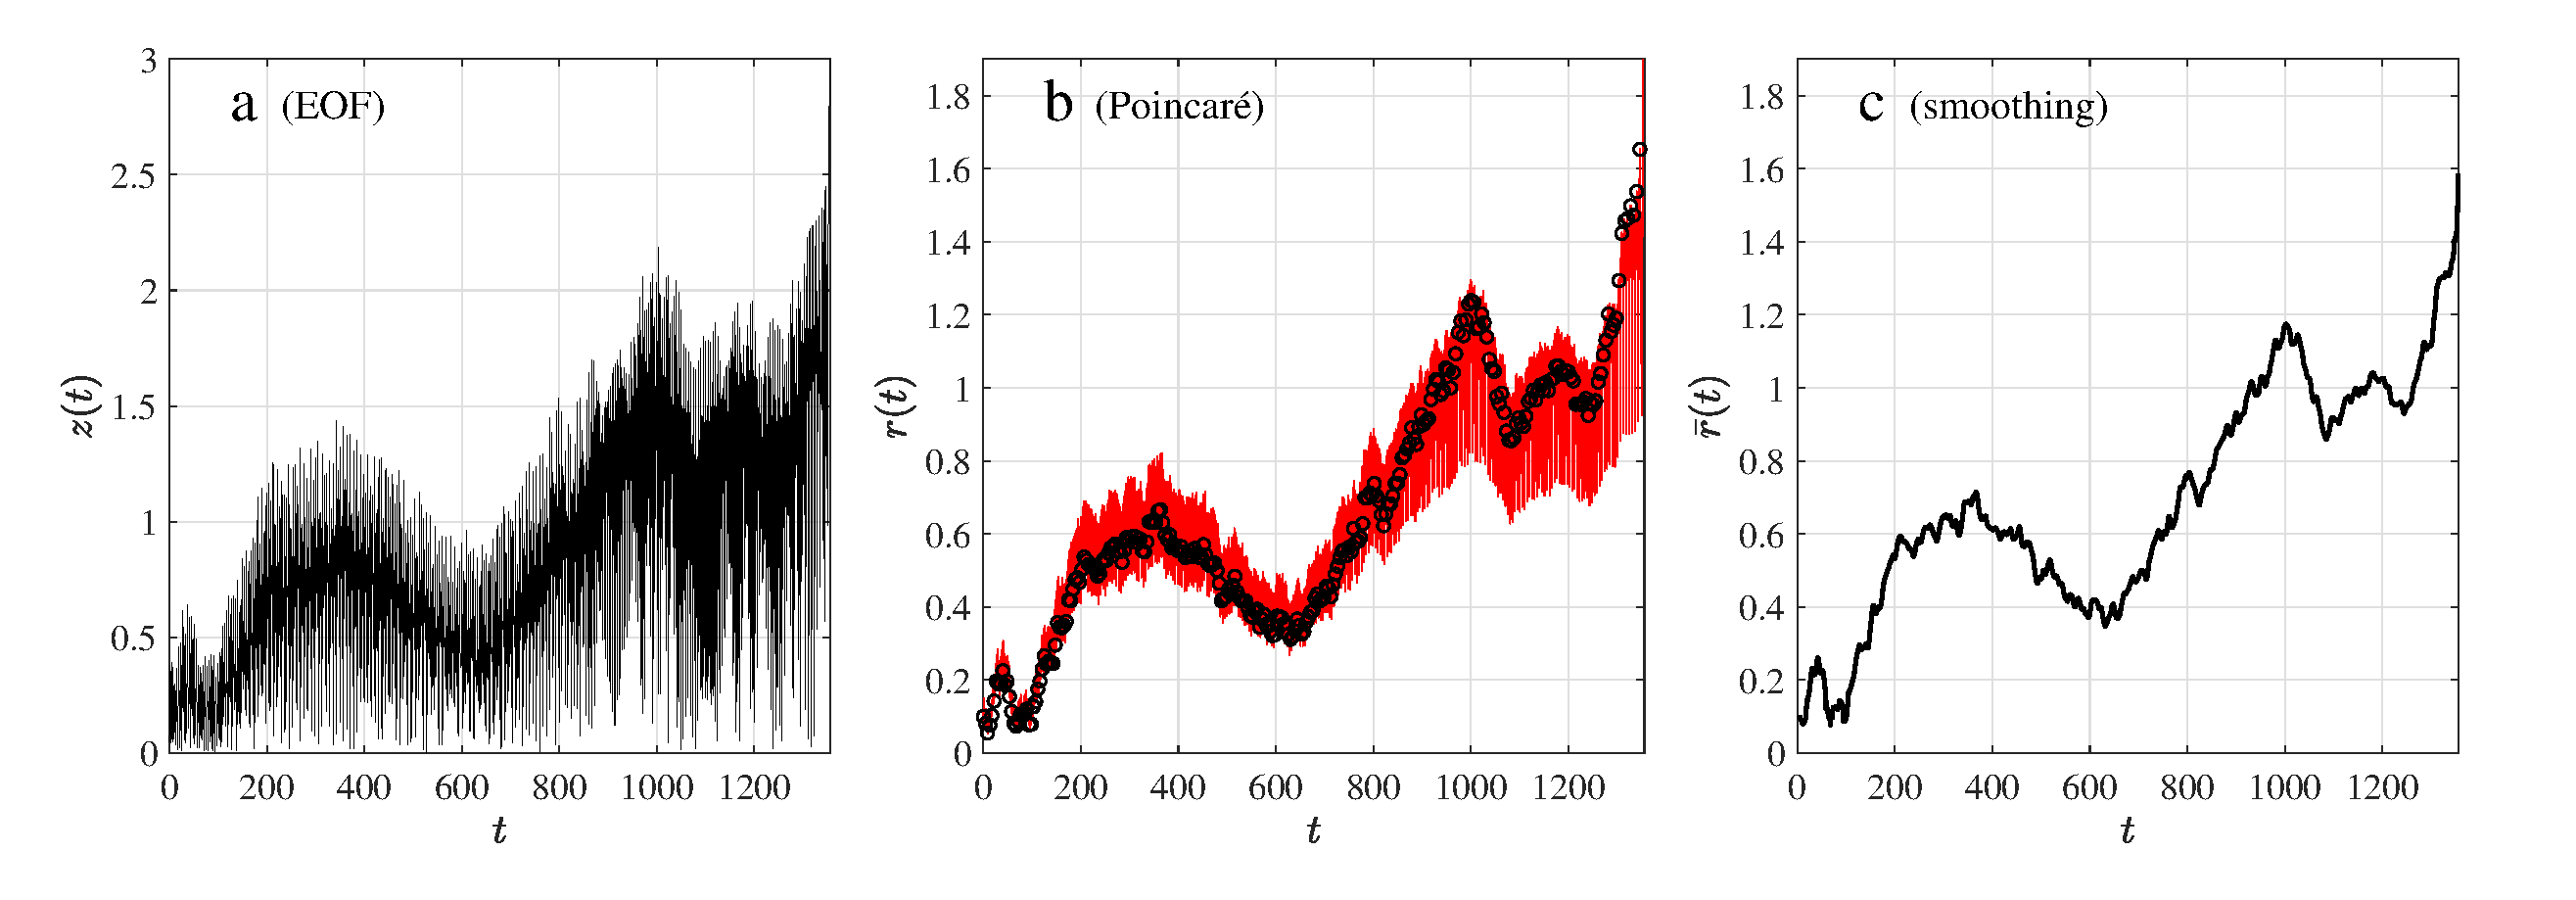
\includegraphics[width = 0.9\columnwidth]{periodicity_3Interpretations}
	\caption{\Red{Three separate interpretations of the System A time series in $x$ and $y$. Panel {\bf a}: the time series are combined using the EOF method to obtain a time series in a single variable. Panel {\bf b}: the radius $R$ (red) and also the Poincar\'{e} map of return points (black circles). Panel {\bf c}: a smoothing applied to the radius where the radius is averaged over each orbit.
	}}
	\label{fig:2D:periodicity:3Interpretations}
\end{figure}


\subsection{Results}
\label{subsec:2D:periodic_orbit:results}
{\Red{
In figure~\ref{fig:2D:periodicity:integration} one integration of System A is presented. We use system equations~\ref{eqn:2D:homoclinicSystem_again} with the standard deviation of both noise terms $\eta^{(x)}$ and $\eta^{(y)}$ set as 0.1. In order to simplify the calculations involved in the two methods described above, we make a simple change of coordinates so that the stable centre is at the origin and the saddle point at $(-2\sqrt{\alpha}, 0)$ is moving towards it as $\alpha$ goes towards zero. Also marked in figure~\ref{fig:2D:periodicity:integration} are the Poincar\'{e} return points, where the system crosses the negative $x$ axis once on each orbit. 

The system is integrated (using the Milstein method) with a time step $\Delta t = 0.01$ in the range $t\in[0,10^4]$, a significantly longer time period than was used in the analysis in section~\ref{sec:2D:MethodsApplied} (see figures~\ref{fig:2D:Homoclinic3D}, \ref{fig:2D:HomoclinicIndicators}). Accordingly, the parameter $\alpha$ is varied more slowly, according to the formula
	\begin{equation}
		\alpha(t) = 1-10^{\m4}t,
	\end{equation}
so that the bifurcation does not occur until $t=10^4$. The initial value of $\alpha$ is therefore $1$, and we use an initial point $(x,y)=(-0.1,0)$ so that the system begins by orbiting the centre at a radius $\approx 0.1$. The observed tipping point therefore occurs earlier than $t=10^4$ since the system will cross the saddle node and `blow up' before the two stable points meet. We disregard any part of the time series after $r>5$. In this particular integration, the system began to diverge at around $t=1400$. 

In figure~\ref{fig:2D:periodicity:3Interpretations} three separate interpretations of the system time series are presented. In panel {\bf a} the time series in $x$ and $y$ are combined using the EOF method to obtain a time series in a single variable. In panel {\bf b} we plot the radius $R$ over time and also the Poincar\'{e} map where the radius is recorded only at the return points. In panel {\bf c}, then, the smoothing method, as described above, has been applied to the data. 

The resulting time series from all three methods were subject to the PS, DFA and ACF1 indicators, as shown in figure~\ref{fig:2D:periodicity:crap_results}. The ACF1 indicator appears to provide the expected EWS when applied to the dimension-reduced, EOF time series, but no clear EWS is observable in any of the indicators applied to the time series produced by either the Poincaré map method or the periodic smoothing technique. 
}}

\begin{landscape}
	\begin{figure}
		\centering
		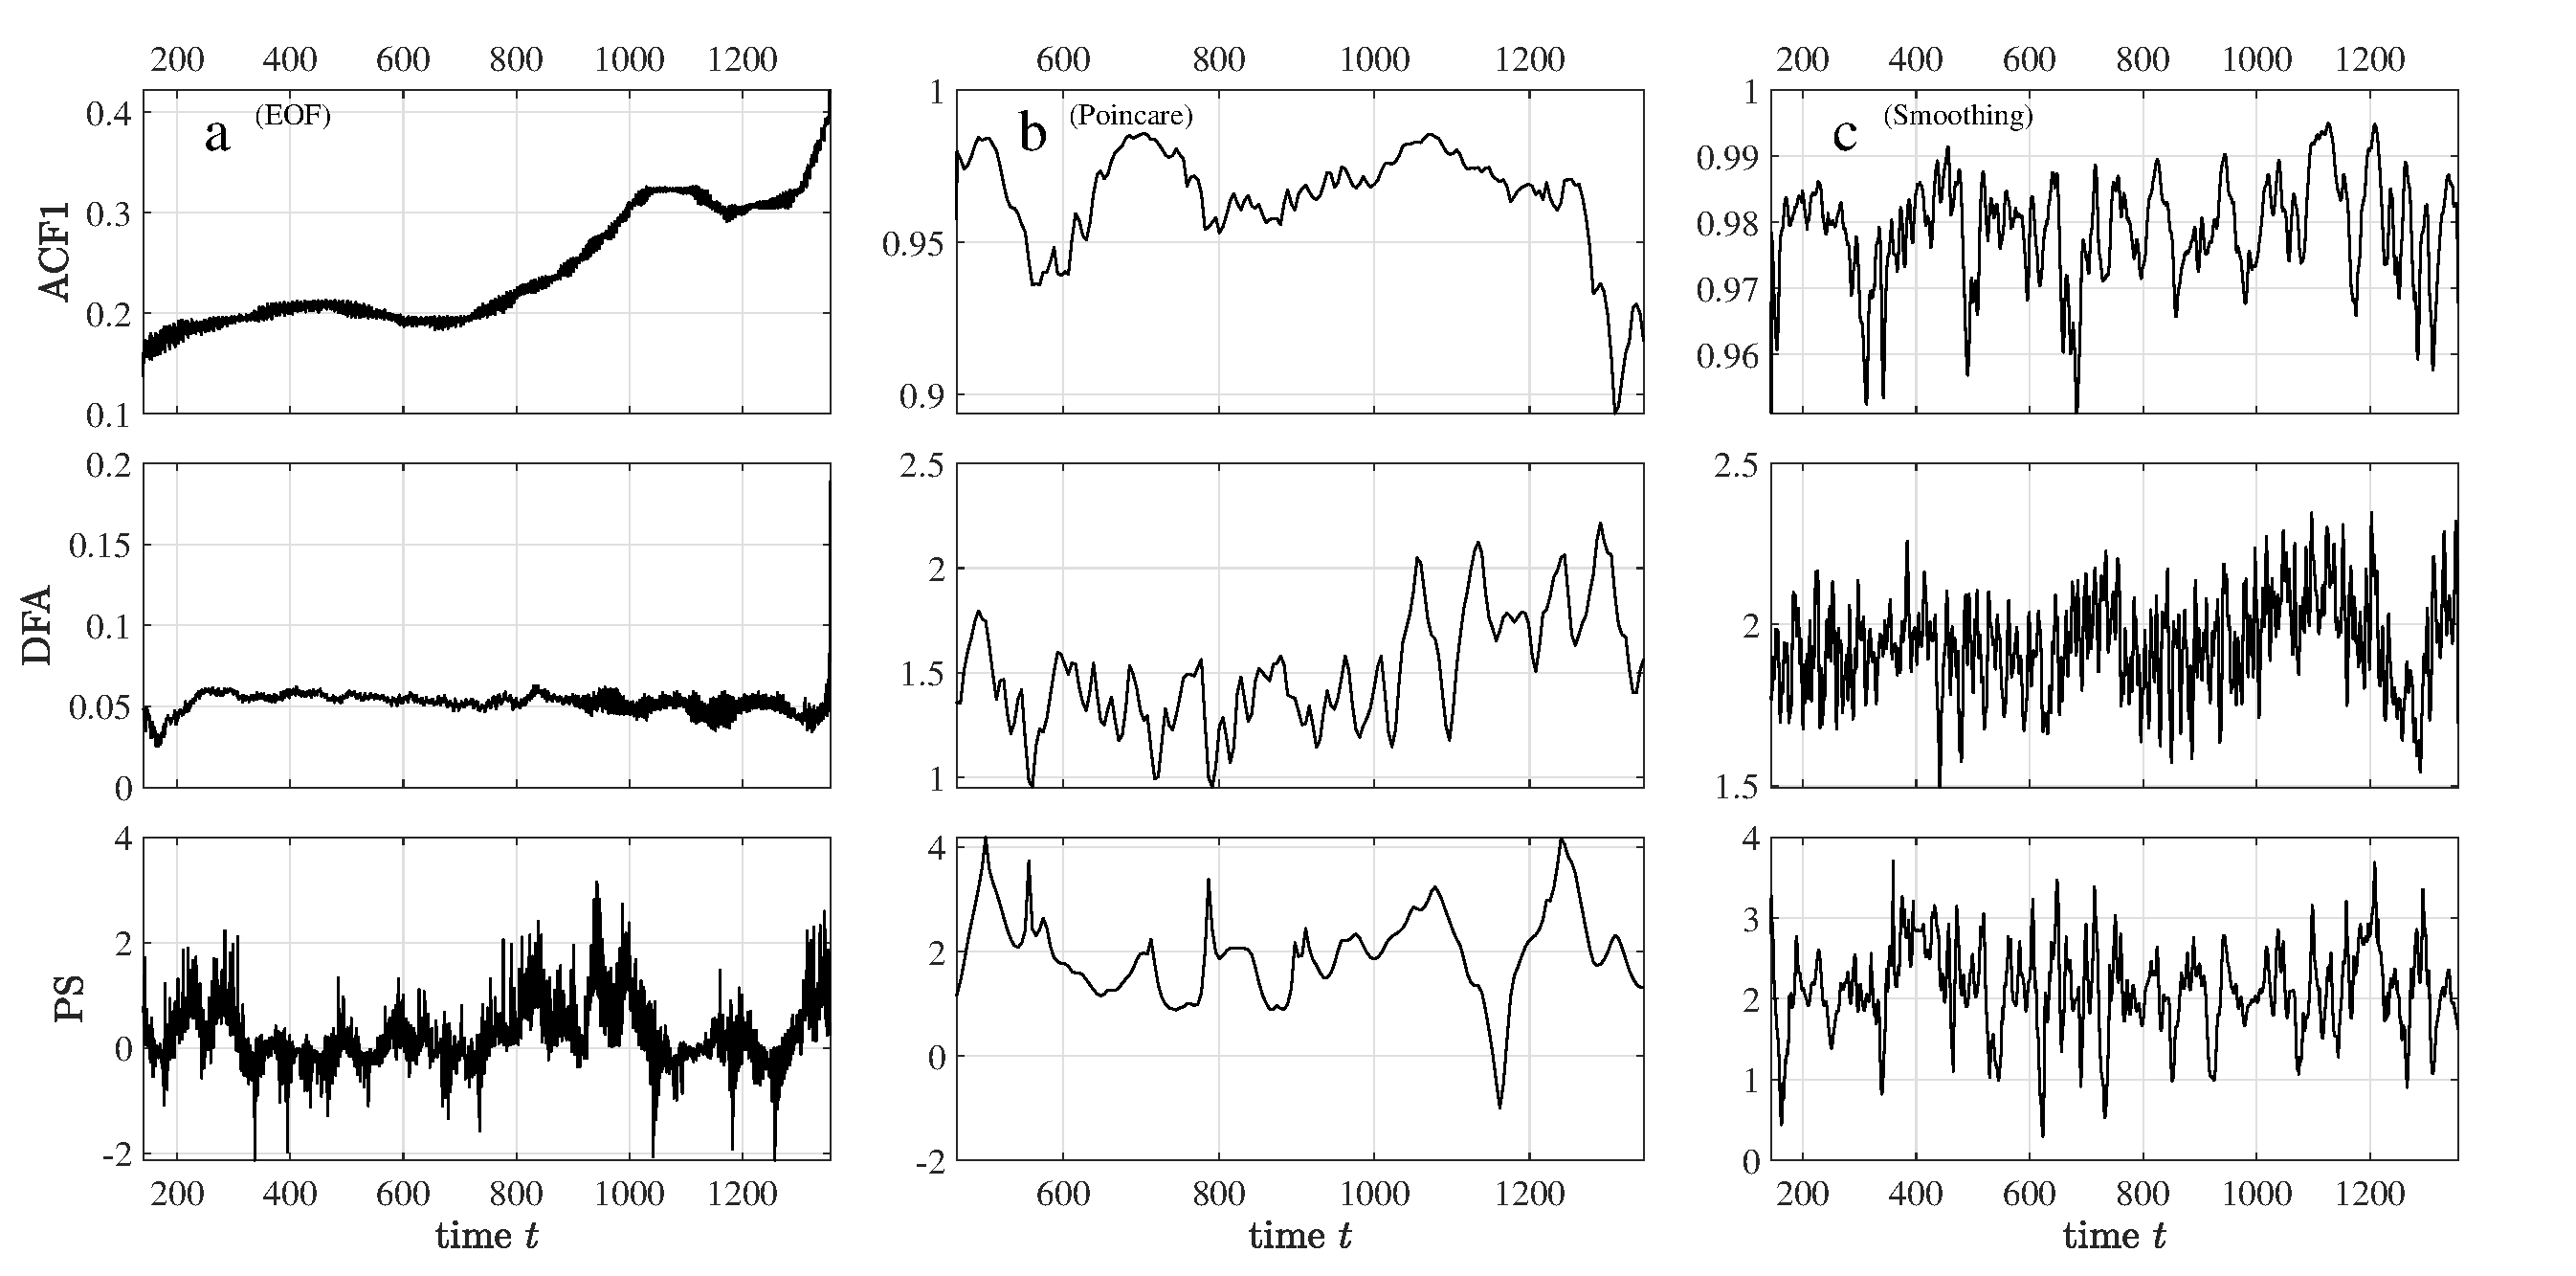
\includegraphics[width=\linewidth,keepaspectratio]{periodicity_results}
		\caption{\Red{ The ACF1 (top row), DFA (middle row) and PS (bottom row) indicators are calculated for the one dimensional time series resulting from each of the three methods illustrated in figure~\ref{fig:2D:periodicity:3Interpretations}: The EOF method (column {\bf a}), the Poincaré map approach (column {\bf b}) and the smoothing applied to the radius (column {\bf c}). We note that neither the Poincaré map nor the smoothing approaches result in any distinguishable EWS in any of the indicators.
		}}
		\label{fig:2D:periodicity:crap_results}
	\end{figure}
\end{landscape}

\section{Justification of EOF dimension reduction}
\label{sec:2D:EOF-justification}

In this section we attempt to justify the use of EOF for dimension reduction in an early warning signal context, as presented in section~\ref{sec:2D:EOF}. By taking the first EOF score of a set of time series, one is projecting on the basis such that the variance is maximised. However, one may favour a dimension which happens to be noisy, having a large variance but no interesting features indicative of a tipping point, whereas viewing the data set along another dimension, which contains lower variability, may yield a useful early warning signal. It is clear that including a single time series composed of white noise with very large variance will make the first EOF score useless. It should be hoped that such cases can be removed before applying the EOF method. However, even in less artificial cases, it is not obvious that viewing a system along a dimension such that the variance is maximised will provide the best EWS in a tipping points context. {\Red{ It may be the case that, in one projection, the variance in the system is large, but constant. In another projection the variance may be small, but \emph{increasing}. The EOF method will give the former projection, since it finds the projection such as to maximise the variance. However, in the context of tipping points, one would of course prefer the latter since it is only the \emph{increase in variance} which can be a useful EWS. The same argument may be made for autocorrelation, if an alternative EOF method sought to maximise autocorrelation rather than variance.
}}

{\Red{The analysis and results presented in this section have previously been presented in \cite{prettyman2019}.}}

\subsubsection{The hypothesis}
\label{sub:EOF-hypothesis}
The essential hypothesis relied upon when using EOF for dimension reduction prior to detecting an EWS, is that the basis in which the variance is maximised (using the EOF method) is similar to the basis in which the \emph{increase in the variance} is maximised. To investigate this hypothesis we consider the $P$-dimensional discrete-time dynamical system $\x_n$ described by 
	\begin{equation}
	\x_{n} = B\x_{n-1} + S\etab_n,
	\label{eqn:EOF-exampleSystem}
	\end{equation}
where $B$, $S$ are symmetric $P\times P$ matrices and the $\etab_n$ are column vectors with each element being independent Gaussian white noise. If $\x$ is one-dimensional ($P=1$), then the system is an AR(1) model. If $P>1$, one may want to study only the first EOF score in the hope that this captures most of the interesting behaviour of the system \citep{held2004}. 

In the simple case where $S$ is the zero matrix, we observe that, as $n$ goes to infinity, for each eigenvalue $\lambda_k$ of $B$ such that $|\lambda_k|<1$, the system goes to zero in the direction of the corresponding eigenvector. Similarly, for each eigenvalue $\lambda_k$ of $B$ such that $|\lambda_k|>1$, the system goes to infinity in the direction of the corresponding eigenvector. 

In this section we consider contracting systems, where all eigenvalues have magnitude less than one. In this case, we have a system which spirals towards zero, and approaches zero fastest in the direction of the eigenvector corresponding to the smallest eigenvalue. We then consider a matrix $B$ constructed such that one of its eigenvalues $\lambda_1$ increases over time, so that there is a tipping point at $\lambda_1=1$ when the system diverges to infinity in the direction of the eigenvector corresponding to $\lambda_1$. It is in the direction of this eigenvector that the tipping point will be most visible and, therefore, projecting the system onto this eigenvector will give the one-dimensional system in which detecting the tipping point will be easiest. If dimension reduction using the EOF method is to be used prior to using one-dimensional EWS methods, one would expect the vector onto which we project the system (the first column of $W$, see section \ref{sec:2D:EOF}), to be in the same direction as the eigenvector of $B$ corresponding to the eigenvalue which is approaching the value one.

This becomes more obvious if we say that $B$ is diagonal, which is equivalent to saying that $B$ is diagonalisable, and $S=0$. Say $B=\text{diag}(b_1, b_2, ..., b_n)$, then $b_1$, $b_2$, ..., $b_n$ are the eigenvalues of $B$ and the system becomes $P$ separate one-dimensional systems,
\begin{equation}
\x_n^{(i)} = b_i^n \x_{n-1}^{(i)}\, ,~~~~~~~ i=1,2,...,P.
\end{equation}
If $b_m = \min_i|b_i|$ the system will go to zero fastest in the direction of the standard basis vector $\mathbf{e}_m$, and we note that $\mathbf{e}_m$ is also the eigenvector of the diagonal $B$ corresponding to the eigenvalue~$b_m$.

\subsection{Analytic calculation of eigenvectors}
\label{sub:EOF-analysis}

In order to test the hypothesis of the EOF method, we calculate the EOF eigenvectors analytically. First, we calculate the empirical mean $\overline{\x}$ of the time series $\{\x_k\}_{k=0}^{N-1}$, defined by equation \ref{eqn:EOF-exampleSystem}, before applying the mean-centring step of the EOF method. We note that the system equation can be rewritten explicitly as
\begin{equation}
\x_k = B^k\x_0 + \sum_{j=0}^{k-1} B^{j} S \etab_{k-s},
\label{eqn:EOF-SytemRewrite1}
\end{equation}
and this can then be further rewritten to remove the dependence on $k$ from the sum:
\begin{align}
	\begin{split}
\x_k &= B^k\x_0 + \left[ \sum_{j=0}^{\infty} B^{j} S \etab_{k-j} - \sum_{j=k}^{\infty} B^{j} S \etab_{k-j}\right]\\
&= B^k\x_0 + \left[ \sum_{j=0}^{\infty} B^{j} S \etab_{k-j} - \sum_{j=0}^{\infty} B^{j+k} S \etab_{-j}\right]\\
&= \sum_{j=0}^{\infty} B^{j} S \etab_{k-j} - B^k \left(\sum_{j=0}^{\infty} B^{j} S \etab_{-j} - \x_0\right).
\label{eqn:EOF-SytemRewrite2}
\end{split}
\end{align}
There remains a dependence on $k$ inside the first sum in equation \ref{eqn:EOF-SytemRewrite2}, but this only affects the noise term and is easier to deal with. We also replace $k$ with $N_0+k$, effectively beginning our analysis of the system after $N_0$ steps, which will allow us to consider the long-term influence of the initial point $\mathbf{x}_0$. Now to find the empirical mean $\overline{\x}$, that is, we take the sum over $k$ in equation \ref{eqn:EOF-SytemRewrite2}:
\begin{align}
\begin{split}
	\overline{\x} &= \frac{1}{N}\sum_{k=0}^{N-1} \x_{N_0+k}\\
	&= \sum_{j=0}^{\infty} B^j S \frac{1}{N}\sum_{k=0}^{N-1}\eta_{N_0+k-j} - B^{N_0} \frac{1}{N}\sum_{k=0}^{N-1} B^k \left(\sum_{j=0}^{\infty} B^{j} S \etab_{-j} - \x_0\right).
\end{split}
\end{align}
Note that $\frac{1}{n}\sum_{k=0}^{n-1}\eta_{N_0+k-j} \rightarrow \mathbb{E}(\eta_0)$ since it is the empirical mean of independent noise terms, in this case the noise is Gaussian with mean zero, so we can ignore the first term. Also note that 
\begin{equation}
\sum_{k=0}^{N-1} B^k = (I-B)^{-1}(I-B^N),
\end{equation}
where $I$ is the identity matrix, thus we can write
\begin{equation}
\frac{1}{N}\sum_{k=0}^{N-1} \x_{N_0+k} =  B^{N_0} \frac{1}{N} (I-B)^{-1}(I-B^N)\left(\x_0 - \sum_{j=0}^{\infty} B^{j} S \etab_{-j} \right).
\label{eqn:EOF-simplifiedMean}
\end{equation}
Taking the $L^2$-norm of each side and noting that $\|I-B^N\|\leq 1$, we obtain
\begin{equation}
\left\|\frac{1}{N}\sum_{k=0}^{N-1} \x_{N_0+k}\right\| \leq \frac{\|B\|^{N_0}}{N} \left( \|(I-B)^{-1}\|\cdot \left\|\x_0 - \sum_{j=0}^{\infty} B^{j} S \etab_{-j} \right\| \right),
\end{equation}
and we note that the part in brackets does not depend on $N$, $N_0$ or $k$. We take the expectation of both sides and define
\begin{equation}
K := \mathbb{E}\left[ \|(I-B)^{-1}\| \left\|\x_0 - \sum_{j=0}^{\infty} B^{j} S \etab_{-j} \right\| \right]
\end{equation}
to say that for any value $c>0$ there is a choice of $N$ and $N_0$ such that
\begin{equation}
\mathbb{E}\left[\overline{\x}\right] \leq K\frac{\|B\|^{N_0}}{N} \leq c.
\end{equation}
With this choice of $N$ and $N_0$, we continue to use $\overline{\x}=0$. In effect, there exists a number $N_0$ such that after this number of iterations, the influence of the initial point $x_0$ is no longer significant. 

The covariance $C$, given by 
\begin{align}
C = \mathbb{E}\left[ \left(\x_{k+N_0} - \mathbb{E}(\x) \right) \left(\x_{k+N_0} - \mathbb{E}(\x) \right)^\top \right],
\end{align}
is calculated using the empirical mean to approximate the expected value as part of the EOF method by taking the sum over $k$. We also use the result $\overline{\x}=0$ to leave
\begin{equation}
C = \frac{1}{N}\sum_{k=0}^{N-1}\left[ (\x_{k+N_0})(\x_{k+N_0})^\top \right].
\label{eqn:EOF-simplifiedCovariance}
\end{equation}
Expanding this using equation \ref{eqn:EOF-SytemRewrite2}, most of the terms are essentially similar to the expression for $\overline{\x}$ and are similarly approximately zero for the same choice of $N$ and $N_0$. This is easily noticed if we simplify the expanded expression using
\begin{align}
\mathbf{p}_k &:= \sum_{s=0}^{\infty} B^{s} S \etab_{k-s}\,,\\
\mathbf{q} &:= \sum_{s=0}^{\infty} B^{s} S \etab_{-s} - \x_0\,,
\end{align}
which allows us to write $\x_k = \mathbf{p}_k - B^k\mathbf{q}$. The terms inside the sum in equation \ref{eqn:EOF-simplifiedCovariance} are then
\begin{equation}
(\mathbf{p}_{k+N_0})(\mathbf{p}_{k+N_0})^\top + B^{k+N_0}\mathbf{q}(B^{k+N_0}\mathbf{q})^\top - B^{k+N_0}\mathbf{q}(\mathbf{p}_{k+N_0})^\top - (\mathbf{p}_{k+N_0}) (B^{k+N_0}\mathbf{q})^\top.
\end{equation}
All terms except for the first involve multiplication by the matrix $B^{k+N_0}\mathbf{q}$, or its transpose. Taking the sum over $k$ gives the same expression for the mean $\overline{\x}$ as in equation \ref{eqn:EOF-simplifiedMean}, and we have chosen $N_0$ such that $\overline{\x}=0$. We now expand the remaining term inside the sum, that is, expand
\begin{equation}
(\mathbf{p}_{k+N_0})(\mathbf{p}_{k+N_0})^\top = \sum_{s=0}^\infty \sum_{r=0}^\infty B^s S(\eta_{k+N_0-s})(\eta_{k+N_0-r})^\top S^\top (B^\top)^r.
\label{eqn:EOF-double_sum_expansion}
\end{equation}
The expected value of the matrix $(\eta_{k+N_0-s})(\eta_{k+N_0-r})^\top$ is the zero matrix for $r\neq s$ and the identity matrix for $r=s$. Therefore
\begin{align}
\mathbb{E}\left[C\right] &= 
\mathbb{E}\left[\sum_{k=0}^{N-1}(\mathbf{p}_{k+N_0})(\mathbf{p}_{k+N_0})^\top\right]\\
&= 
\sum_{k=0}^{N-1}\mathbb{E}\left[(\mathbf{p}_{k+N_0})(\mathbf{p}_{k+N_0})^\top\right]\\
&= \sum_{k=0}^{N-1}\sum_{s=0}^\infty B^s S S^\top (B^\top)^s\\
&= \sum_{s=0}^\infty B^s S S^\top (B^\top)^s.
\label{eqn:EOF-covarianceFinal}
\end{align}

In the special case that $B = \text{diag}(b_1, b_2, ...)$ and $S = \text{diag}(s_1, s_2, ...)$, we are able to calculate the entire matrix component-wise to get
\begin{align}
\mathbb{E}([C]_{ii}) &= s_i^2\frac{1}{N-1}\sum_{r=1}^{N}\sum_{t=1}^{r} b_i^{2(t-r)}\\
&= s_i^2\frac{1}{N-1}\sum_{r=0}^{N-1}(N-r)b_i^{2r} \\
&= s_i^2\sum_{r=0}^{N}b_i^{2r} - s_i^2\sum_{r=0}^{N}\frac{r-1}{N-1}b_i^{2r}\\
&= s_i^2\sum_{r=0}^{\infty}b_i^{2r} - s_i^2\sum_{r=0}^{\infty}\frac{r-1 - (r+1)b^{2(N+1)}}{N-1}b_i^{2r}.
\end{align}
However, when substituting these diagonal matrices into our expression for the covariance matrix in equation \ref{eqn:EOF-covarianceFinal} we get simply
\begin{align}
\mathbb{E}([C]_{ii}) = s_i^2\sum_{r=0}^\infty b_i^{2r}.
\end{align}
This is because our working introduced the $N_0$ term in order to ignore the first terms of the series and approximate the mean as zero. It should be noted that equation \ref{eqn:EOF-covarianceFinal} is therefore only a first approximation to the covariance. 

We also note that the same calculation can be done with a time lag so that we are finding the covariance of $\x_k$ and $\x_{k+l}$. In this case the equation \ref{eqn:EOF-double_sum_expansion} becomes
\begin{align}
(\mathbf{p}_{k+N_0})(\mathbf{p}_{k+l+N_0})^\top = \sum_{s=0}^\infty \sum_{r=0}^\infty B^s S(\eta_{k+N_0-s})(\eta_{k+l+N_0-r})^\top S^\top (B^\top)^r,
\end{align}
and the expected value of the matrix $(\eta_{k+N_0-s})(\eta_{k+l+N_0-r})^\top$ is equal to the identity matrix when $r = s+l$, rather than $r=s$, and zero otherwise. So we have simply 
\begin{equation}
\mathbb{E}(C_{\text{lag-}l}) = \mathbb{E}\left[(\mathbf{p}_{k+N_0})(\mathbf{p}_{k+l+N_0})^\top\right] = \sum_{s=0}^\infty B^s S S^\top (B^\top)^{s+l},
\end{equation}
which is the same matrix as the regular (lag-0) covariance given in equation \ref{eqn:EOF-covarianceFinal} but right-multiplied by $(B^l)^\top$. For simplicity, we call this matrix $D$:
\begin{equation}
D:=\mathbb{E}(C) = \sum_{s=0}^\infty B^s S S^\top (B^\top)^s.
\end{equation}
This equation allows us to define $D$ intrinsically as
\begin{equation}
D = SS^\top + B D B^\top,
\end{equation}
which we can then solve component-wise. In the fairly trivial one-dimension case $d=s^2+b^2d$ we have 
\begin{equation}
d = \frac{s^2 }{1-b^2}\,.
\end{equation}
In two-dimensions we restrict our study to the case where $B$ is diagonal, which is equivalent to asking that $B$ is diagonalisable. We obtain
\begin{equation}
	D = \left[ 
	\begin{array}{cc}
	\frac{s_{12}^2+s_{11}^2}{1-b_{11}^2} & \frac{s_{12}s_{22}+s_{11}s_{21}}{1-b_{11}b_{22}}\\
	\frac{s_{12}s_{22}+s_{11}s_{21}}{1-b_{11}b_{22}} & \frac{s_{22}^2+s_{21}^2}{1-b_{22}^2}
	\end{array}
	\right],
\label{eqn:2D:B_diag}
\end{equation}
and are able to examine the eigenvalues easily because of its symmetry. The eigenvalues of a general symmetric $2\times 2$ matrix 
\begin{equation}
\left(
\begin{array}{cc}
a&b\\
b&c
\end{array}
\right)
\end{equation}
are 
\begin{equation}
\frac{1}{2}\left(a+c\pm\sqrt{(a-c)^2+4b^2}\right),
\label{eqn:EOF-generalEigenvalues}
\end{equation}
and we can see that, when matrix $D$ is substituted into this, the positive square root will give the largest (principal) eigenvalue. Note that for $b=0$ (i.e. the matrix is diagonal) the difference between the two eigenvalues is $|a-c|$, but for non-zero $b$ this difference increases, i.e. the eigenvalues become more distinct. Matrix $D$ is diagonal when two entries of $S$ are zero, not in the same column, in which case the system (equation \ref{eqn:EOF-exampleSystem}) is simply two separate AR(1) models. The eigenvector corresponding to the largest eigenvalue (taking the positive root) is 
\begin{equation}
\left[\begin{array}{c}
\frac{s_{12}^2+s_{11}^2}{1-b_{11}^2}-\frac{s_{22}^2+s_{21}^2}{1-b_{22}^2} + \sqrt{\left(\frac{s_{12}^2+s_{11}^2}{1-b_{11}^2}-\frac{s_{22}^2+s_{21}^2}{1-b_{22}^2}\right)^2+4\left(\frac{s_{12}s_{22}+s_{11}s_{21}}{1-b_{11}b_{22}}\right)^2}\\
~\\
2\left(\frac{s_{12}s_{22}+s_{11}s_{21}}{1-b_{11}b_{22}}
\right)
\end{array}\right].
\label{eqn:EOF-2x2eigenvector}
\end{equation}
This is the principal eigenvector used in the EOF method; the assumption is that projecting onto this eigenvector, which maximises variance, captures the interesting behaviour of the system. For the purpose of tipping point analysis, we would therefore expect that this eigenvector has something to do with the eigenvector corresponding to the largest eigenvalue of $B$ (closest to one), since this is the direction in which the system travels slowest to zero. A bifurcation occurs when one eigenvalue approaches one. 

Without loss of generality, we assume that the first eigenvalue of $B$ is approaching one; since $B$ is diagonal this is equal to the first entry of $B$, $b_{11}$, and the corresponding eigenvector is the standard basis vector $\mathbf{e}_1 = [1,0]^\top$.
We make the choice that $b_{11}\approx 1$ (from below), then 
$1-b_{11}$ is very small. We are therefore inclined to expand the terms in the principal eigenvector (equation~\ref{eqn:EOF-2x2eigenvector}) in leading order terms of $(1-b_{11})$, allowing us simplify the expression by ignoring negligible terms. The objective is to expand the square root
\begin{equation}
	Q := \sqrt{\left(\frac{s_{12}^2+s_{11}^2}{1-b_{11}^2}-\frac{s_{22}^2+s_{21}^2}{1-b_{22}^2}\right)^2+4\left(\frac{s_{12}s_{22}+s_{11}s_{21}}{1-b_{11}b_{22}}\right)^2}.
\end{equation}
To simplify the working we make the following substitutions:
	\begin{align}
	\begin{split}
		\varepsilon &:=1-b_{11},\\
		p &:= s_{11}^2+s_{12}^2,\\
		q &:= s_{21}^2+s_{22}^2, \\
		r &:= s_{12}s_{22}+s_{11}s_{21}.
	\end{split}
	\end{align}
The expression then becomes
	\begin{align}
	\begin{split}
		Q =& \sqrt{\left(\frac{p}{\varepsilon(1+b_{11})}-\frac{q}{1-b_{22}^2}\right)^2+4\left(\frac{r}{1-(1-\varepsilon) b_{22}}\right)^2}\\
		=& \frac{1}{\varepsilon}\sqrt{\frac{p^2}{(1+b_{11})^2}-\varepsilon\frac{2pq}{(1+b_{11})(1-b_{22}^2)}-\varepsilon^2\frac{q^2}{(1-b_{22}^2)^2}+\varepsilon^2\frac{4r^2}{(1-(1-\varepsilon) b_{22})^2}} \,\, .
	\end{split}
	\end{align}
Concentrating on the final term inside the square root, we use the Taylor expansion of $1/(1+x)$ to obtain
	\begin{align}
	\begin{split}
		\frac{1}{1-(1-\varepsilon) b_{22}} &= 1+(1-\varepsilon) b_{22}+(1-\varepsilon)^2 b_{22}^2+...\\
		&=\frac{1}{1-b_{22}} -
		\varepsilon\sum_{k=1}^\infty kb_{22}^k + \varepsilon^2\sum_{k=2}^\infty\left(\begin{array}{c}	k\\2\end{array}\right)b_{22}^k + \mathcal{O}(\varepsilon^3) \,\, ,
	\end{split}
	\end{align}
	and therefore
	\begin{equation}
		\varepsilon^2\frac{4r^2}{(1-(1-\varepsilon) b_{22})^2} = \varepsilon^2\frac{4r^2}{(1-b_{22})^2}+\mathcal{O}(\varepsilon^3) \,\, .
	\end{equation}
Then we can return to our square root:
{\small
	\begin{align}
	\begin{split}
		Q&= \frac{1}{\varepsilon}\sqrt{\frac{p^2}{(1+b_{11})^2}-\varepsilon\frac{2pq}{(1+b_{11})(1-b_{22}^2)}+\varepsilon^2\left[ \frac{4r^2(1+ b_{22})^2 -  q^2 }{(1-b_{22}^2)^2} \right] + \mathcal{O}(\varepsilon^3)}\\
		&= \frac{p}{\varepsilon (1+b_{11})} \sqrt{1+\varepsilon\frac{-2q(1+b_{11})}{p(1-b_{22}^2)}+\varepsilon^2(1+b_{11})^2\left[ \frac{4r^2(1+ b_{22})^2 -  q^2 }{p^2(1-b_{22}^2)^2} \right] + \mathcal{O}(\varepsilon^3)}\\
		&= \frac{p}{\varepsilon (1+b_{11})}\left[1+
		\varepsilon\frac{-q(1+b_{11})}{p(1-b_{22}^2)}+\varepsilon^2\frac{(1+b_{11})^2}{2}\left[ \frac{4r^2(1+ b_{22})^2 -  q^2 }{p^2(1-b_{22}^2)^2}\right] - 
		\right. \\
		& \qquad\qquad\qquad\qquad\qquad\qquad\qquad\qquad\qquad \quad \left.
		-\frac{1}{8}\left(\varepsilon\frac{-2q(1+b_{11})}{p(1-b_{22}^2)} \right)^2 + \mathcal{O}(\varepsilon^3)
		\right] \\
		&= \frac{p}{\varepsilon (1+b_{11})}\left[1+
		\varepsilon\frac{-q(1+b_{11})}{p(1-b_{22}^2)}+
		\varepsilon^2 \left[ \frac{4r^2(1+ b_{22})^2(1+b_{11})^2 -  q^2(1+b_{11})^2 }{2p^2(1-b_{22}^2)^2}\right] \right. \\
		&\qquad\qquad\qquad\qquad\qquad\qquad\qquad\qquad\qquad  \qquad\left.
		-\varepsilon^2\left[\frac{q^2(1+b_{11})^2}{2p^2(1-b_{22}^2)^2}\right]
		+ \mathcal{O}(\varepsilon^3)
		\right]\\
		&= \frac{p}{\varepsilon (1+b_{11})}\left[1+
		\varepsilon\frac{-q(1+b_{11})}{p(1-b_{22}^2)}+
		\varepsilon^2(1+b_{11})^2 \left[ \frac{4r^2(1+ b_{22})^2 -  2q^2 }{2p^2(1-b_{22}^2)^2}\right]
		+ \mathcal{O}(\varepsilon^3)
		\right]\\
		&=
		\frac{p}{\varepsilon (1+b_{11})} + 
		\frac{-q}{(1-b_{22}^2)}+
		\varepsilon(1+b_{11}) \left[ \frac{2r^2(1+ b_{22})^2 -  q^2 }{p(1-b_{22}^2)^2}\right]
		+ \mathcal{O}(\varepsilon^2)\\
		&=
		\frac{p}{(1-b_{11}^2)} + 
		\frac{-q}{(1-b_{22}^2)}+
		(1-b_{11}^2) \left[ \frac{2r^2(1+ b_{22})^2 -  q^2 }{p(1-b_{22}^2)^2}\right]
		+ \mathcal{O}(\varepsilon^2).
	\end{split}
	\end{align}
}
We can now substitute this expansion of $Q$ for the square root term in the first component of the principal eigenvector (equation~\ref{eqn:EOF-2x2eigenvector}), which becomes
	\begin{equation}
		\frac{2p}{(1-b_{11}^2)} + 
		\frac{-2q}{(1-b_{22}^2)}+
		(1-b_{11}^2) \left[ \frac{2r^2(1+ b_{22})^2 -  q^2 }{p(1-b_{22}^2)^2}\right]
		+ \mathcal{O}((1-b_{11})^2),
	\end{equation}
or simply
	\begin{equation}
		\frac{2p}{(1-b_{11}^2)} + 
		\frac{-2q}{(1-b_{22}^2)}
		+ \mathcal{O}((1-b_{11})).
	\end{equation}
A similar treatment of the second eigenvector component yields
	\begin{align}
		\frac{2r}{1-b_{11}b_{22}} & = 2r\left[\frac{1}{1-b_{22}} -
		\varepsilon\sum_{k=1}^\infty kb_{22}^k + \varepsilon^2\sum_{k=2}^\infty\left(\begin{array}{c}k\\2\end{array}\right)b_{22}^k + \mathcal{O}(\varepsilon^3)
		\right]\\
		& = 2r\left[\frac{1}{1-b_{22}} -
		\varepsilon\frac{b_{22}}{(1-b_{22})^2}
		\right]
		+ \mathcal{O}(\varepsilon^2)\\
		& = \frac{2r(1 - 2b_{22} + b_{11}b_{22})}{(1-b_{22})^2}
		+ \mathcal{O}((1-b_{11})^2)\\
		& = \frac{2r}{1-b_{22}}+ \mathcal{O}((1-b_{11})).
	\end{align}
Thus, if we ignore terms in $\mathcal{O}(1-b_{11})$, the principal eigenvector in equation~\ref{eqn:EOF-2x2eigenvector} becomes
\begin{equation}
\left[\frac{s_{12}^2+s_{11}^2}{1-b_{11}^2}-\frac{s_{22}^2+s_{21}^2}{1-b_{22}^2} ~,~\frac{s_{12}s_{22}+s_{11}s_{21}}{1-b_{22}}
\right]^\top,
\label{eqn:2D:EOFeigenVector}
\end{equation}
which, since $1/(1-b_{11}^2)$ is very large, is approximately equivalent to $[1,0]^\top$ as expected. If $S$ is diagonal ($s_{12}=s_{21}=0$) then the vector is actually equivalent to $[1,0]^\top$, in this situation the two system variables are actually separate one-dimensional AR(1) models, since $B$ is also diagonal. However, if $s_{11},s_{12}$ are very small and $s_{21},s_{22}$ are very large, it may not be true that the eigenvector is approximately in the direction $[1,0]^\top$. This implies that there is very large variability in the second component of the system (in the direction of $[0,1]^\top$), and so this exception is predicted by our knowledge of the EOF method. 

We have considered the expected value of the covariance matrix, since the noise will cause every realisation of the system to be different. This analysis is also intended to tell us something general about the validity of using dimension reduction by the EOF method prior to using tipping point analysis techniques. The method must be valid where the entries of $S$ are large, giving large variability due to noise, or in situation when given time series data of unknown origin which resembles the output of the general system in equation~\ref{eqn:EOF-exampleSystem}. In these situations the covariance matrix $C$ obtained from the data by the EOF method may be significantly different to the expectation $D = \mathbb{E}(C)$, in which case it may be uncertain which is truly the principal eigenvalue, especially when the eigenvalues are very similar. Equation~\ref{eqn:EOF-generalEigenvalues} tells us that the difference between the eigenvalues is smallest when the covariance matrix is diagonal, i.e. when the system is reducible to separate AR(1) models, and that the difference increases as the off-diagonal entries of $S$ increase, i.e. as the system becomes more strongly coupled.

\subsection{Numerical verification}
\label{sub:EOF-verification}
The analysis in section \ref{sub:EOF-analysis} makes some assumptions to aid the calculations. In particular, only two-dimensional systems are considered when calculating the eigenvectors of the covariance matrix. In this section we provide numerical experiments to further validate the conclusions of section \ref{sub:EOF-analysis} and also to provide some insight into three- and four-dimensional systems. 

\subsubsection{Two-dimensional system}
We first consider the two-dimensional system 
\begin{equation}
\x_{k} = \Lambda\x_{k-1} + S\etab_k,
\label{eqn:EOF-2DbasicSystem}
\end{equation}
where $\etab_k$ is a white noise vector and $\Lambda=\text{diag}(\lambda_1, \lambda_2)$ is diagonal. $\lambda_2 = 0.9$ and $\lambda_1$ is made to approach one from below:
\begin{equation}
	\lambda_1(k) = 0.9+10^{-6}k,
\end{equation}
so that $\lambda_1=\lambda_2$ at $k=0$, and at $k=10^5$ a bifurcation occurs as the system tips from convergence to divergence, diverging to infinity in the $x$-direction, i.e. in the direction of $(\pm 1,0)^\top$. In the previous section we concluded that the nature of the matrix $S$, specifically the values on the off-diagonal, determines the effectiveness of the EOF method in this context. As an illustration, we initially consider two extreme cases: 
\begin{enumerate}
	\item The two variables are entirely uncoupled:\begin{equation}
	\label{eqn:2D:uncoupledMatrix}
		S_1 = \frac{1}{20}\left(\begin{array}{cc}
		1 & 0 \\
		0 & 1
		\end{array}\right).
	\end{equation}
	\item The two variables are coupled:\begin{equation} 
	\label{eqn:2D:coupledMatrix}
		S_2 = \frac{1}{20}\cdot\frac{1}{\sqrt{2}}\left(\begin{array}{cc}
		1 & 1 \\
		1 & 1
		\end{array}\right).
	\end{equation}
\end{enumerate}
 The factor $1/\sqrt{2}$ in $S_2$ is to ensure that the standard deviation of the noise is the same in both cases. Na\"ively, we may expect that the leading EOF eigenvector will be similar to $(\pm 1,0)^\top$ since this is the direction in which the divergence happens, or, before the bifurcation, the direction in which the convergence is weakest and therefore the direction with the longest recovery time after a perturbation from the equilibrium. This may be true eventually but not when $\lambda_1$ and $\lambda_2$ are very close. According to equation~\ref{eqn:EOF-2x2eigenvector}, the eigenvector, when using the identity matrix $S_1$, will be 
\begin{equation}
	\left[\begin{array}{c}
	\frac{1}{1-\lambda_1^2}-\frac{1}{1-0.9^2}\\
	0
	\end{array}\right],
\label{eqn:2D:S1expected_eigenvector}
\end{equation}
which is in the direction $(\pm 1,0)^\top$ for $\lambda_1\neq 0.9$, but is the zero vector when $\lambda_1= 0.9$. At this point, the EOF eigenvector is determined only by the noise, and therefore the angle of that vector will be random in the range $[-\pi/2, \pi/2]$, with mean zero. The angle will tend to zero (i.e. the EOF eigenvector will approach $(1,0)^\top$) as the difference $|\lambda_1-0.9|$ is sufficiently large that the EOF method is able to distinguish the effect upon the system from the noise. 

When using the matrix $S_2$ we will have the vector
\begin{equation}
\left[\begin{array}{c}
\frac{1}{1-\lambda_1^2}-\frac{1}{0.19} + \sqrt{\left(\frac{1}{1-\lambda_1^2}-\frac{1}{0.19}\right)^2+\left(\frac{2}{1-0.9\lambda_1}\right)^2}\\
~\\
\frac{2}{1-0.9\lambda_1}
\end{array}\right]\,,
\label{eqn:2D:S2expected_eigenvector}
\end{equation}
which is in the direction $(1,1)^\top$ for $\lambda_1=0.9$ and approaches $(1,0)^\top$ as $\lambda_1\rightarrow 1$ as the $1/(1-\lambda_1^2)$ term becomes very large. The angle of this vector will therefore start as $\theta_\text{eig} = \pi/4$ when $k=0$ (i.e. $\lambda_1=0.9$) and tends towards zero as $k$ increases. 

Using both of these matrices $S_1$ and $S_2$ we calculate the terms $\x_k$ up to the point of the bifurcation ($k=10^5$). For each of the resulting series we perform the EOF analysis on 200 half-overlapping segments of length $10^3$, in order to see how the EOF eigenvectors change as $k$ increases. In each segment the angle variable of the EOF eigenvector is calculated.

Figure~\ref{fig:2D:EOFtest_extreme_simple} shows the result when using $S_1$ (panel \textbf{a}) and $S_2$ (panel \textbf{b}). 
\begin{figure}
	\centering
	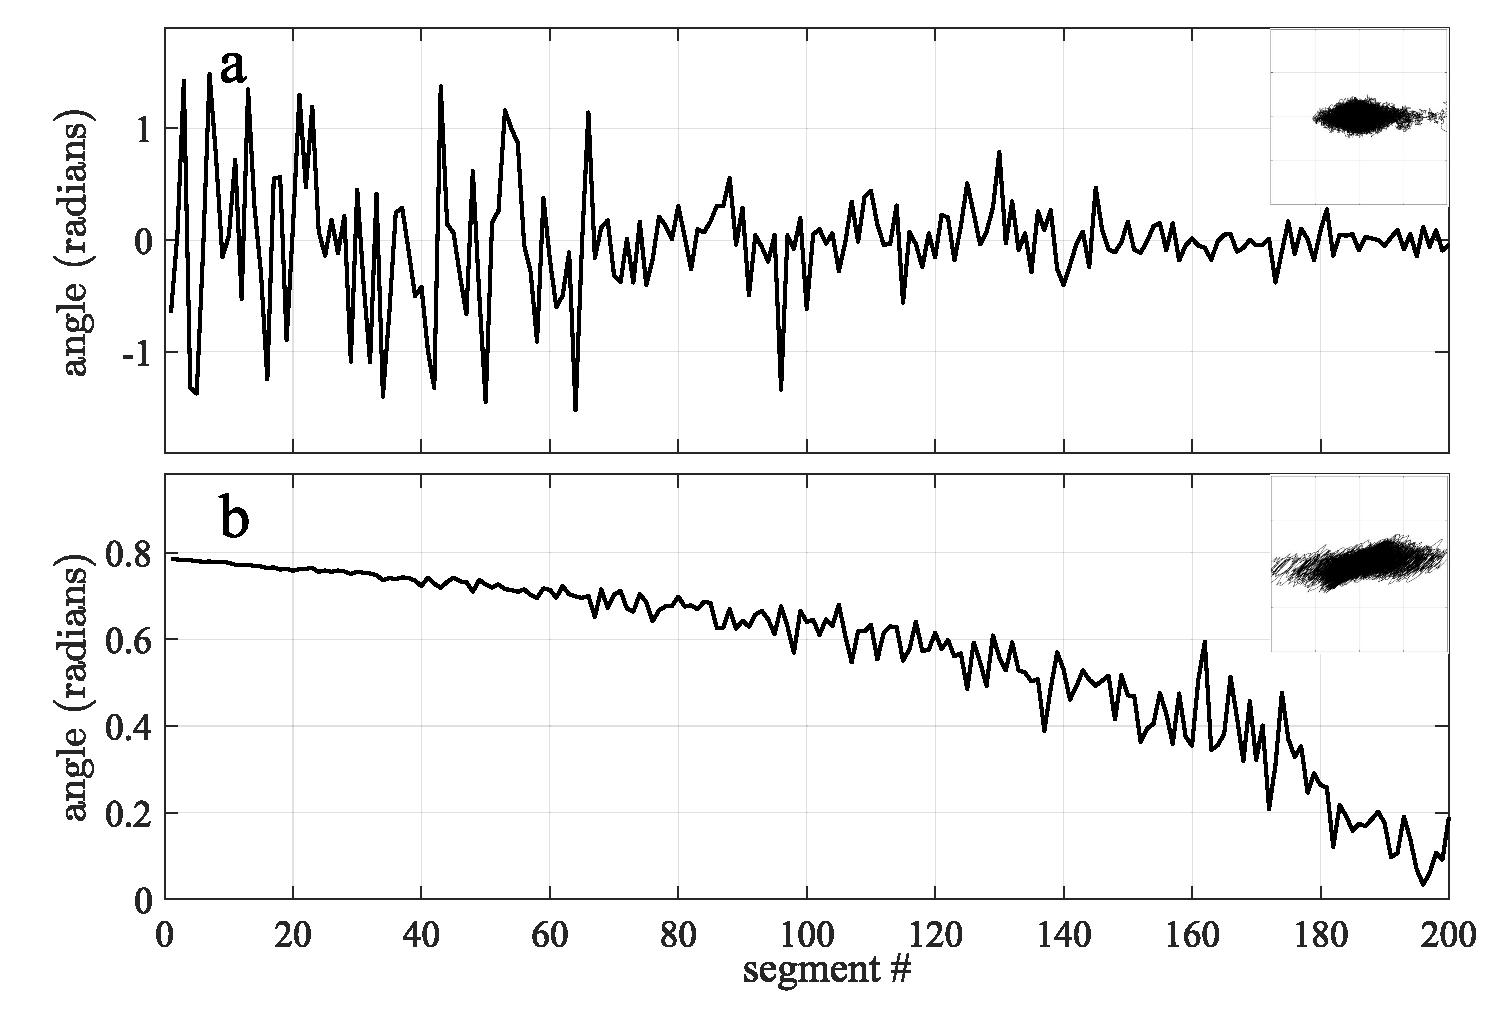
\includegraphics[width = 0.9\columnwidth]{EOFtest_extreme_simple2}
	\caption{The angle variable of the EOF eigenvector calculated in 200 overlapping segments of length $10^3$. Two cases of the system in equation~\ref{eqn:EOF-2DbasicSystem} are considered: using $S_1$ (panel \textbf{a}) and using $S_2$ (panel \textbf{b}), see equations~\ref{eqn:2D:uncoupledMatrix} and~\ref{eqn:2D:coupledMatrix}. The series itself is plotted, in each case, in the insert at the top-right of the panel, both $x$ and $y$ axes range from $-2$ to $2$.
		\label{fig:2D:EOFtest_extreme_simple}}
\end{figure}
We see that the nature of the matrix $S$ does affect the EOF projection. When the two systems are uncoupled (i.e. the two variables are two separate AR(1) models) the angle of the eigenvector is apparently random at first when $\lambda_1$ is close to the value $0.9$ but the angle converges towards zero as $\lambda_1$ goes to 1, as predicted. When the two variables are coupled, the angle variable of the EOF eigenvector starts at $\pi/2$ (for $\lambda_1=0.9$) and tends towards zero, also as predicted. 

We now perform the same analysis using a range of 30 intermediate symmetric matrices
\begin{equation}
	S^{(\phi)} = \frac{1}{20}\left(\begin{array}{cc}
	\cos(\phi) & \sin(\phi) \\
	\sin(\phi) & \cos(\phi)
	\end{array}\right),
\end{equation}
where $\phi$ varies from zero (giving the identity matrix $S_1$) to $\pi/4$ (giving the ones matrix $S_2$). For each of the 30 matrices $S^{(\phi)}$ the series $\x_k$ is calculated and the EOF eigenvector angle is found in three segments: one at the start of the series where $\lambda_1$ is close to 0.9 ($k\in[1\times 10^4,2\times 10^4]$); one in the middle of the series ($k\in[4.5\times 10^4,5.5\times 10^4]$); and one close to the bifurcation ($k\in[8\times 10^4,9\times 10^4]$). This is repeated ten times to overcome the effect of noise, and only the absolute value of the angle variable is recorded. The result is shown in figure~\ref{fig:2D:EOFtest_changeS}.
\begin{figure}
	\centering
	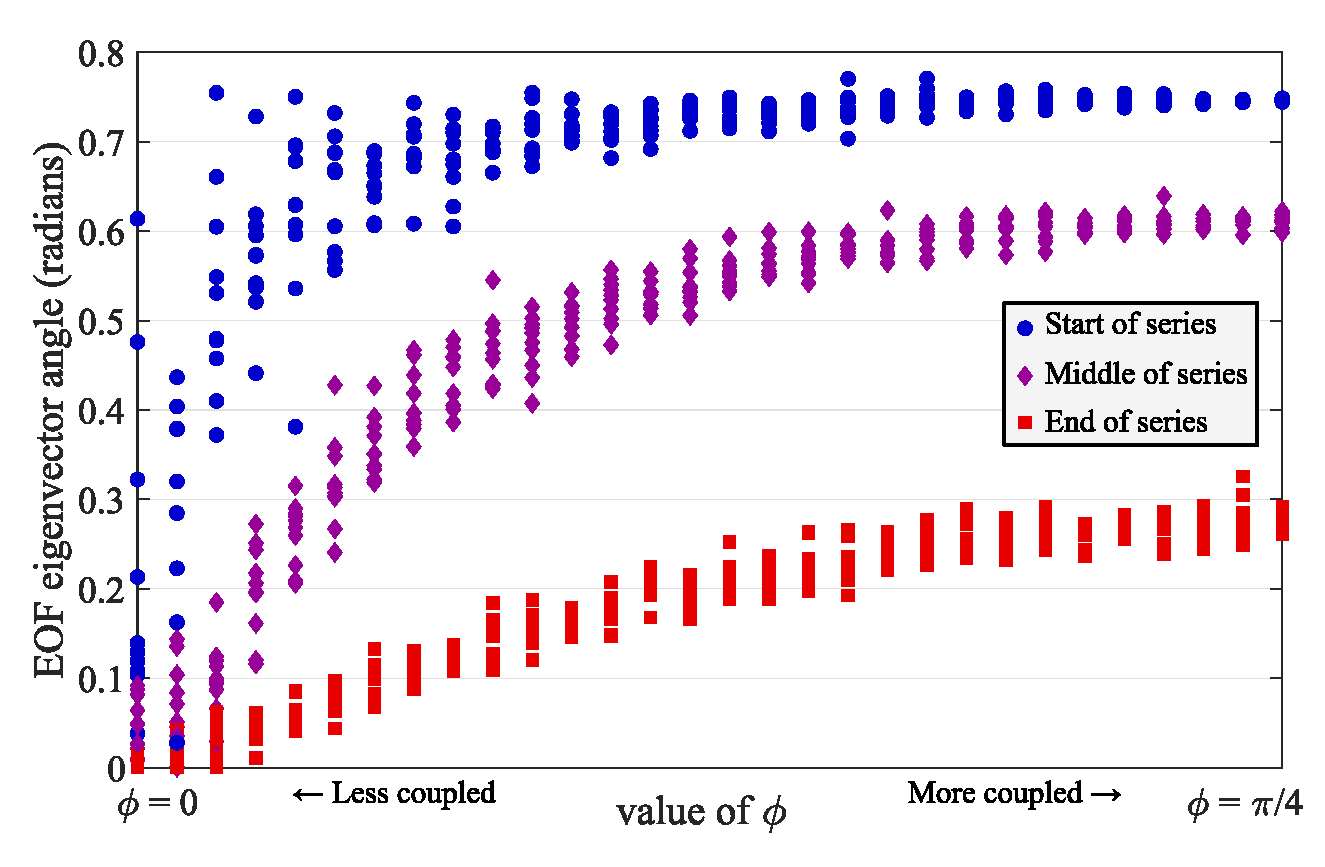
\includegraphics[width = 0.9\columnwidth]{EOFtest_changeS}
	\caption{The absolute value of the angle variable of the EOF eigenvector calculated in three segments of the series $\x_k$ (start, middle and end) using a range of matrices $S^{(\phi)}$. The series is calculated 10 times for each matrix $S^{(\phi)}$, showing the range of angles, particularly for low values of $\phi$ where the system variables are uncoupled.
		\label{fig:2D:EOFtest_changeS}}
\end{figure}
We see that the results at $\phi = 0$ (matrix $S_1$) and $\phi=\pi/4$ (matrix $S_2$) are similar to the results shown in figure~\ref{fig:2D:EOFtest_extreme_simple}, bearing in mind that, this time, the absolute angle is recorded. However, in the case of the uncoupled system (small $\phi$) there is less variability here at the start of the series than seen in figure~\ref{fig:2D:EOFtest_extreme_simple}. Rather than being distributed in the range $[0,\pi/2]$, the ‘start of series' points, which correspond to the same values of $k$ as segments numbered $20$ to $40$ in figure~\ref{fig:2D:EOFtest_extreme_simple}, do not exceed $0.8$. This is because of the larger sample used: $10^4$ points rather than $10^3$ points. Repeating the figure~\ref{fig:2D:EOFtest_extreme_simple} analysis with a larger segment size, we note that this results in a more accurate EOF projection since, with a larger sample, the effect of the system eigenvalues of the convergence or divergence is more easily distinguishable from the noise. 

We note that after about half way along the horizontal axis ($\phi>\pi/8$) there is almost no change in any of the segments. Most of the qualitative change occurs over the first six values of $\phi$ used, that is $\phi<\pi/20$, which leads us to consider the matrix 
	\begin{equation}
		S^{(\pi/20)} = \frac{1}{20}\left(\begin{array}{cc}
		0.988 & 0.156 \\
		0.156 & 0.988
		\end{array}\right).
	\end{equation}
At this level of noise (standard deviation = $1/20$) the degree to which the system variables are coupled does not qualitatively affect the EOF method beyond this point. 

\subsubsection{Three-dimensional system}
We now perform the same analysis as above with equation~\ref{eqn:EOF-2DbasicSystem} being a three dimensional system, that is, $\Lambda=\text{diag}(\lambda_1, \lambda_2, \lambda_2)$. In this system $\lambda_2 = 0.9$, and $\lambda_1$ is made to approach one from below:
	\begin{equation}
		\lambda_1(k) = 0.9+10^{-6}k\,.
	\end{equation}
We use the matrices $S_1 = \sigma I$ and $S_2 = \sigma(1/\sqrt{3}) J$ where $I$ is the identity matrix, $J$ is the ones matrix and $\sigma=1/20$ is the standard deviation. Again, the series $\x_k$ is calculated up to $k=10^5$ and the EOF eigenvector is found in overlapping sections of length 1000. This time the angle recorded is necessarily the absolute angle between the EOF eigenvector and $(1,0,0)^\top$, since a negative angle does not make sense in three dimensional space. The result is shown in figure~\ref{fig:2D:EOFtest3D_simple}. 
	\begin{figure}
		\centering
		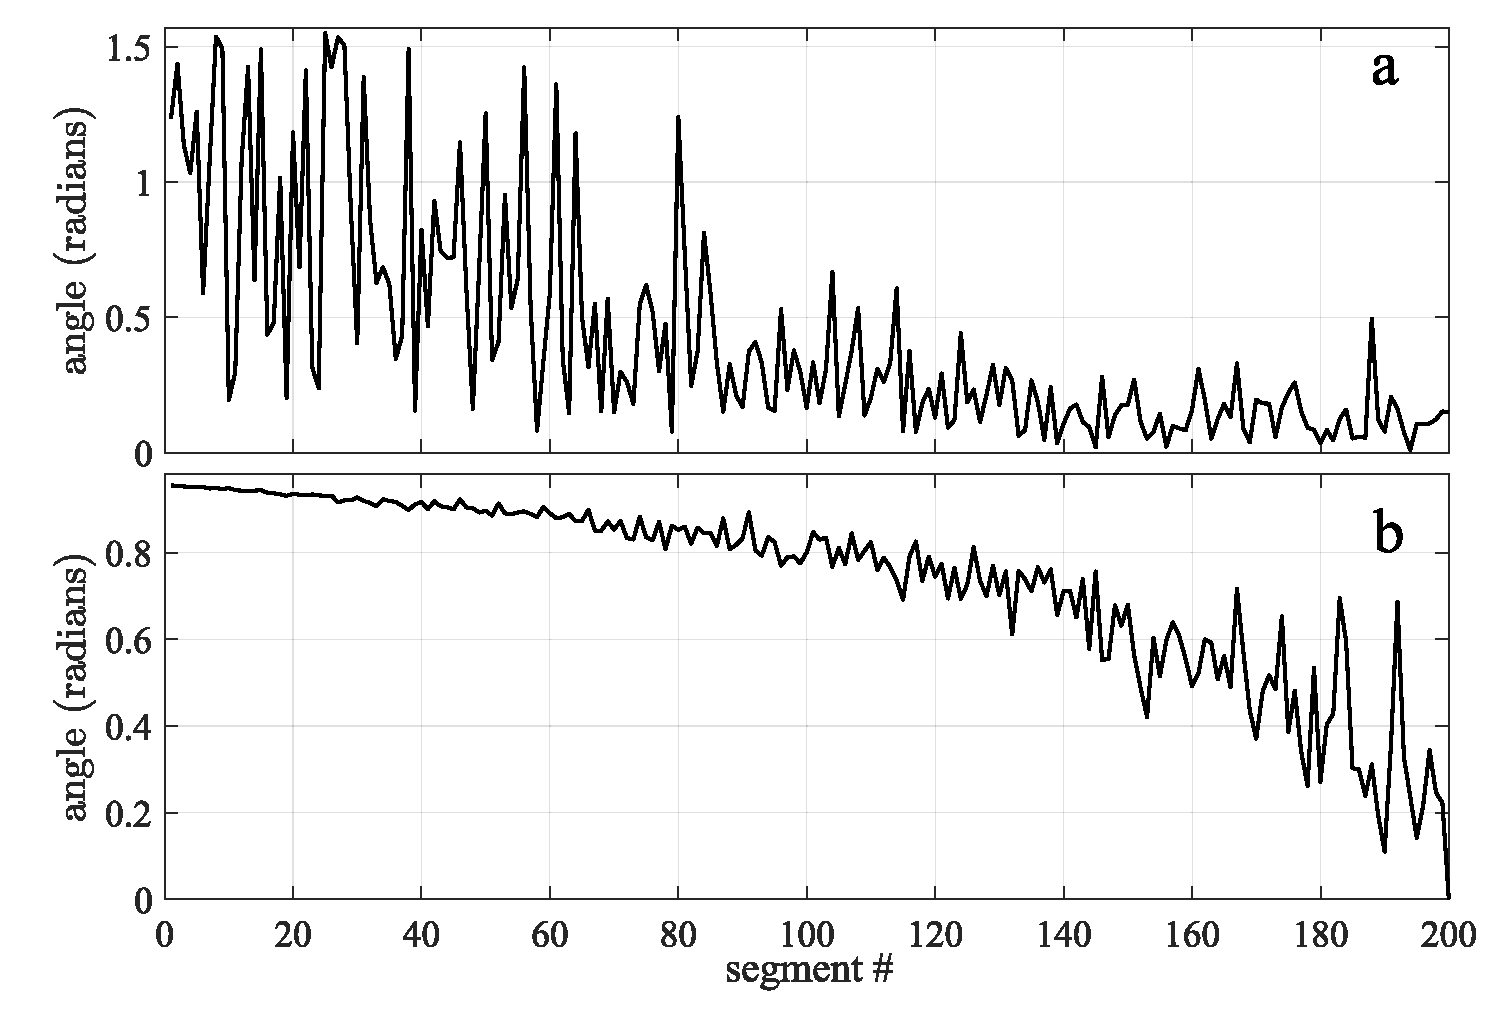
\includegraphics[width = 0.9\columnwidth]{EOFtest3D_simple}
		\caption{The angle variable of the EOF eigenvector calculated in 200 overlapping segments of length $10^3$. Two cases of the three-dimensional system in equation~\ref{eqn:EOF-2DbasicSystem} are considered: using $S_1$ (panel \textbf{a}) and using $S_2$ (panel \textbf{b}).
			\label{fig:2D:EOFtest3D_simple}}
	\end{figure}
We note the obvious similarity to figure~\ref{fig:2D:EOFtest_extreme_simple}, bearing in mind (looking at panel \textbf{a}) that the absolute value of the angle is now considered, so that the random angle will be distributed in the range $[0,\pi/2]$, and (looking at panel \textbf{b}) that the angle made by the vector $(1,1,1)^\top$ is $\arccos(1/\sqrt{3}) = 0.9553...$ which is the angle of the EOF eigenvector when $\lambda_1=0.9$. It appears that there is greater variability in the $S_2$ case close to the end of the series, but the general pattern is the same.

As a further confirmation we also repeat the analysis behind figure~\ref{fig:2D:EOFtest_changeS} using a three-dimensional system. We use the general $3\times 3$ matrix $S^{(\phi)}$ which has $\cos(\phi)$ on the diagonal and $\sin(\phi)/\sqrt{2}$ everywhere else:
	\begin{equation}
		S^{(\phi)} = \frac{1}{20}\left(\begin{array}{ccc}
		\cos(\phi) & \frac{1}{\sqrt{2}}\sin(\phi) & \frac{1}{\sqrt{2}}\sin(\phi)  \\
		\frac{1}{\sqrt{2}}\sin(\phi) & \cos(\phi) & \frac{1}{\sqrt{2}}\sin(\phi)  \\
		\frac{1}{\sqrt{2}}\sin(\phi) & \frac{1}{\sqrt{2}}\sin(\phi) & \cos(\phi) \\
		\end{array}\right).
	\end{equation}
Similarly to the two-dimensional case, as $\phi$ increases from zero to $\arctan(\sqrt{2})$ the matrix $S^{(\phi)}$ changes from $S_1$, which gives an uncoupled system of separate AR(1) models, to $S_2$, which gives a system with an identical noise term in all three variables. The same steps to produce figure~\ref{fig:2D:EOFtest_changeS} are followed in the three-dimensional case and the result is shown in figure~\ref{fig:2D:EOFtest3D_changeS}.
	\begin{figure}
		\centering
		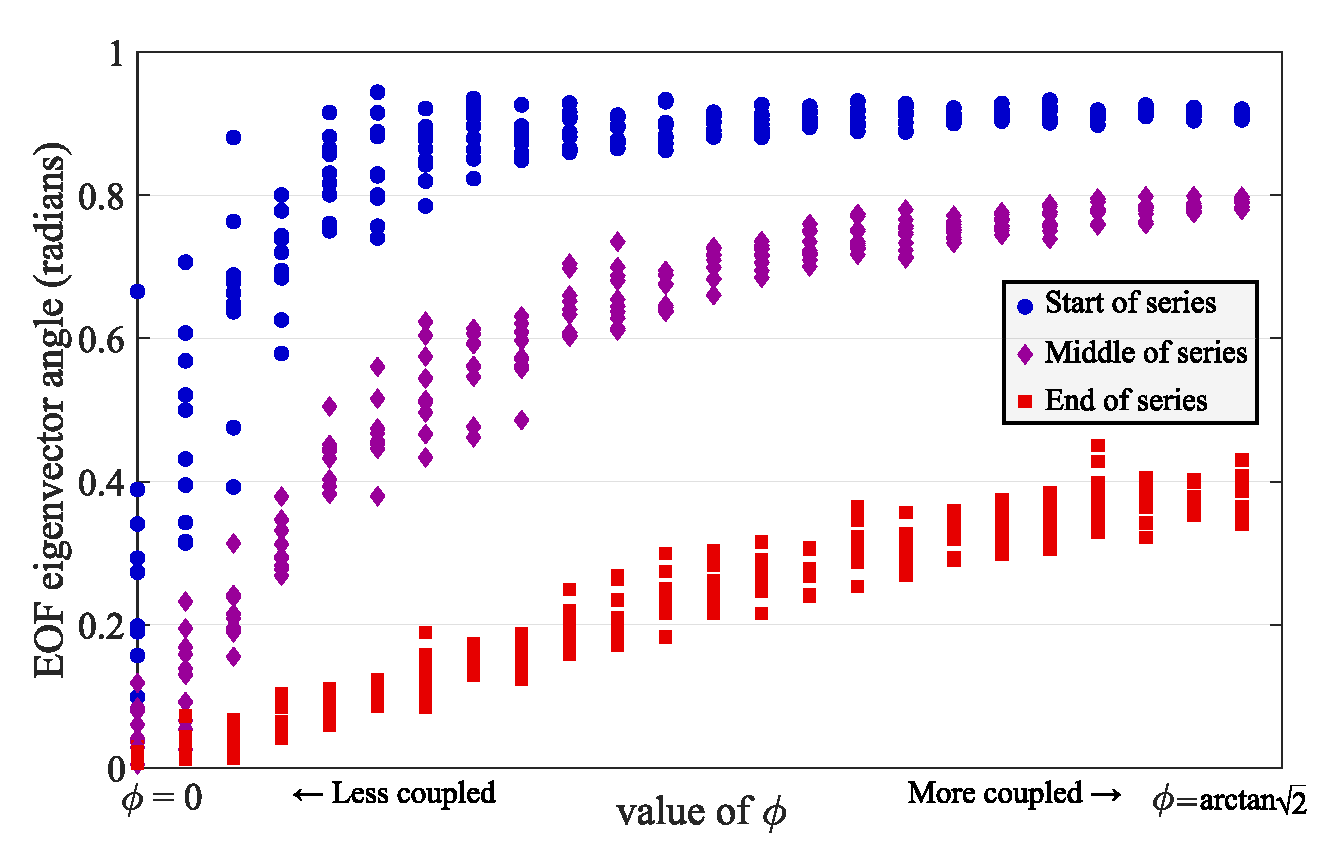
\includegraphics[width = 0.9\columnwidth]{EOFtest3D_changeS}
		\caption{The absolute value of the angle variable of the EOF eigenvector calculated in three segments of the three-dimensional series $\x_k$ (start, middle and end) using a range of $3\times 3$ matrices $S^{(\phi)}$. The series is calculated 10 times for each matrix $S^{(\phi)}$, showing the range of angles.
			\label{fig:2D:EOFtest3D_changeS}}
	\end{figure}
We note, as with the two-dimensional case, that the EOF method is more accurate at the start of the more uncoupled system series in this figure, where the segment sampled is $10^4$ points, than in figure~\ref{fig:2D:EOFtest3D_simple} where the segment size is $10^3$ points. We also note again that the EOF eigenvector at the start of the coupled system series is in the direction $(1,1,1)^\top$ with an angle $\arccos(1/\sqrt{3}) = 0.9553$ rather than $\arccos(1/\sqrt{2}) = \pi/4$ as in the two-dimensional case (from the direction $(1,1)^\top$). Again, there is very little change after about half way along the horizontal axis ($\phi>\arctan(\sqrt{2})/2$) and most of the qualitative change occurs over the first five or six values of $\phi$ used here ($\phi<0.2$). 

\subsubsection{Higher dimensions}


This same analysis is applied to higher dimensional systems where the matrix $S$ is given by the general formula
\begin{equation}
	S^{(\phi)} = 
	\frac{1}{20}\left(I_p\cos(\phi) + (J_p-I_p)\frac{\sin(\phi)}{\sqrt{p-1}} \right)\,,
\end{equation}
where $I$ is the identity matrix, $J$ is the ones matrix, and $p$ is the dimension of the system. In this way, the system changes from an uncoupled system of separate AR(1) models ($S=\sigma I$) to a coupled system ($S=\sigma J$) as $\phi$ increases from zero to $\phi_\mathrm{max}$, given by
\begin{equation}
\phi_\mathrm{max} = \arctan\left(\sqrt{p-1}\right).
\end{equation}

The results, presented similarly to the $p=3$ results in figure~\ref{fig:2D:EOFtest3D_changeS}, are shown for $p=4$ and $p=5$ in figure~\ref{fig:2D:EOFtest_changeS_4D}. We note that there is little qualitative difference as the dimension increases. 

	\begin{figure}
		\centering
		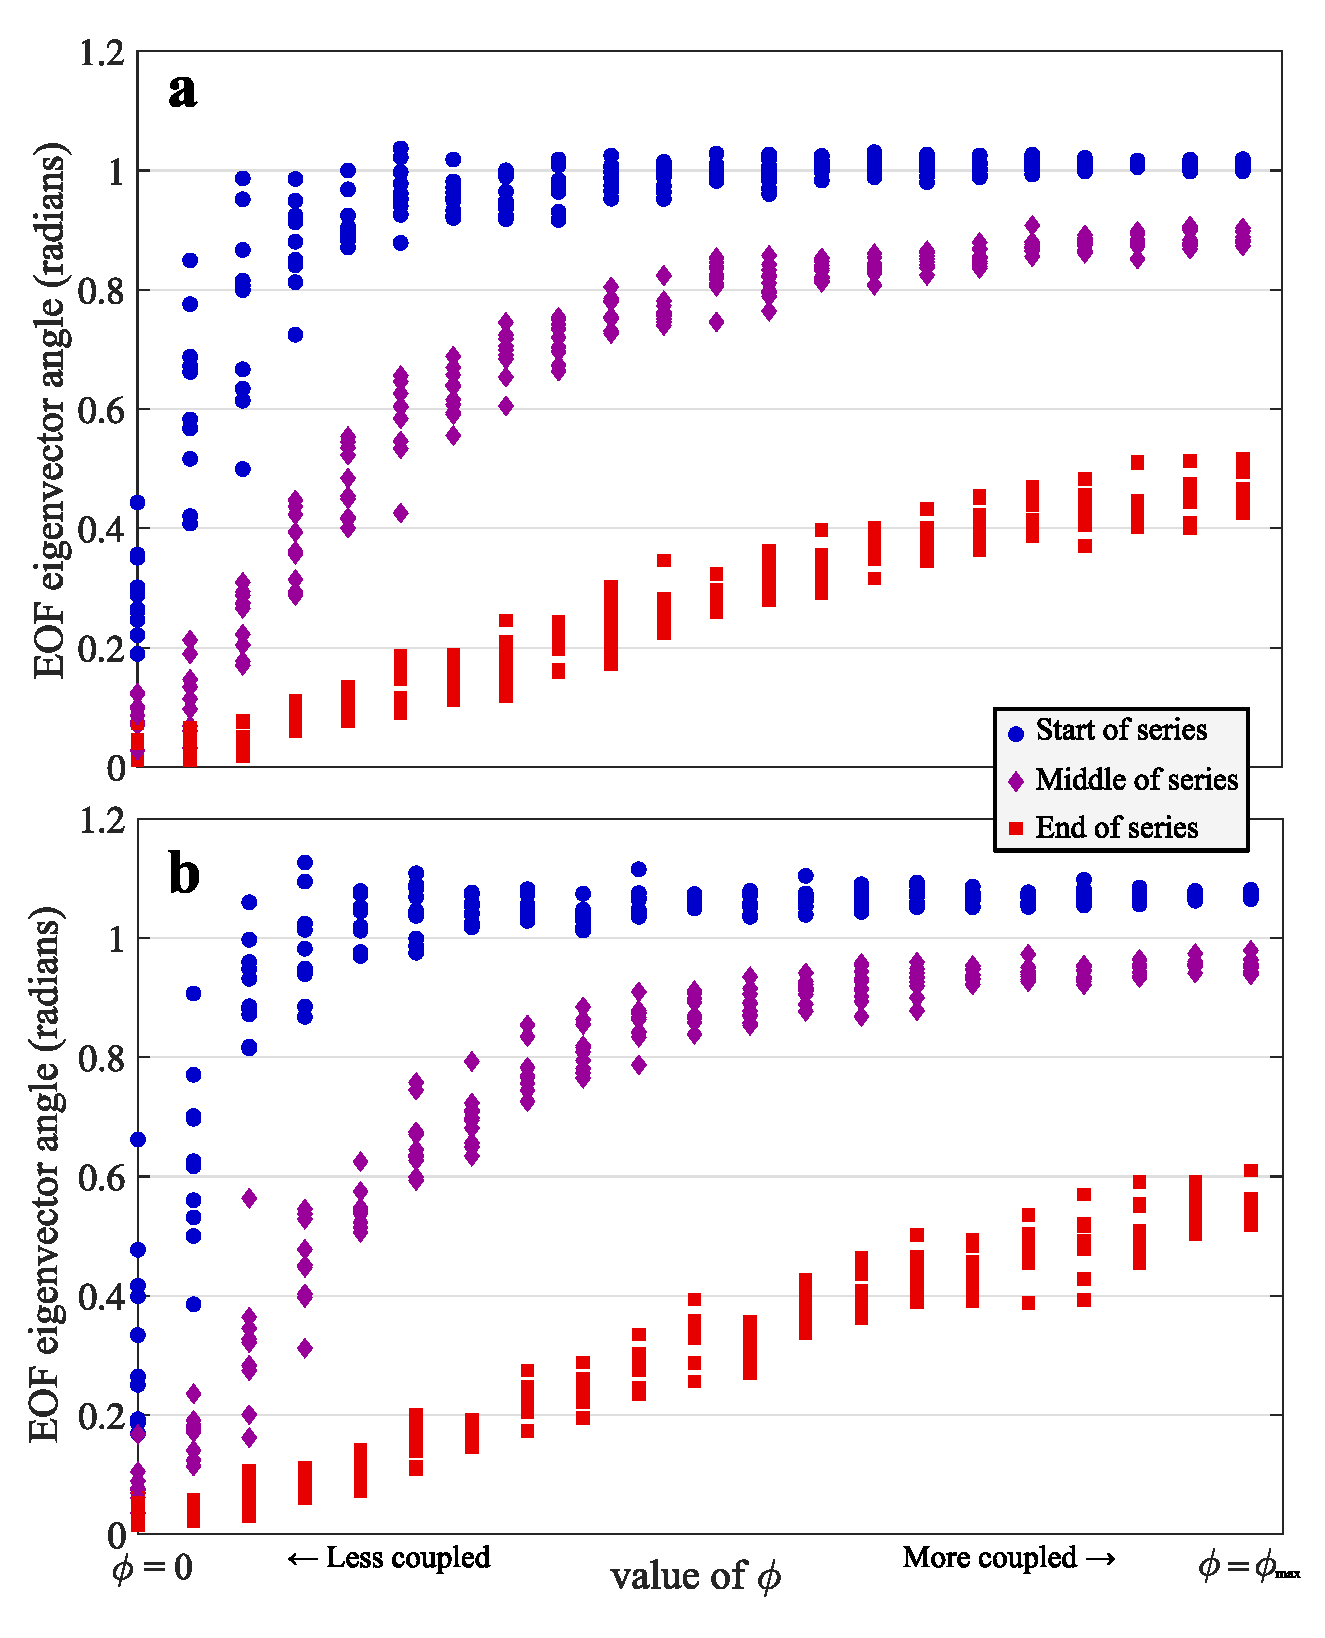
\includegraphics[width = 0.9\columnwidth]{EOFtest_changeS_4D}
		\caption{
			For four-dimensional (panel \textbf{a}) and five-dimensional (panel \textbf{b}) systems, the absolute value of the angle variable of the EOF eigenvector calculated in three segments of the series $\x_k$ (start, middle and end) using a range of $n\times n$ matrices $S^{(\phi)}$. In both cases, the series is calculated 10 times for each matrix $S^{(\phi)}$, showing the range of angles.
		\label{fig:2D:EOFtest_changeS_4D}}
	\end{figure}



\section{An alternative EOF method for dimension reduction}
\label{sec:2D:AlternativeEOF}

Although the EOF method is widely used in ecology and geosciences \citep{hasselmann1988,dommenget2001,bathiany2013p1} occasionally, even, in the process of detecting EWSs \citep{held2004}, it is not ideally suited for this purpose because it does not take into account the internal dynamics of the system. \cite{dommenget2001} note:
	\begin{quote}
		... EOF analyses have problems in identifying the dominant centres of action or the teleconnections between these centres of action in multivariate datasets. We therefore have to be very careful in interpreting the EOF modes as potential physical modes. 
	\end{quote}
\cite{hasselmann1988} proposes that the use of principal interaction patterns and principal oscillation patters (PIPs and POPs) \citep{von1995,kwasniok1996} is much better suited to applications where the evolution of a system over time is relevant, including EWS applications. The PIP technique is introduced by \cite{hasselmann1988} as an alternative to EOF analysis for reducing the dimension of a system to ``a few dominant patterns'', with the benefit that the system dynamics are modelled, similarly to an ARMA parametrisation. The use of PIPs and POPs may therefore be used to reduce the dimension of a system prior to applying one-dimensional tipping point indicators, as an alternative to EOFs. 

Besides these shortcomings, which lead one to favour PIPs and POPs as an alternative, we have noted (section~\ref{sec:2D:EOF-justification}) that it may not necessarily be the case that the EOF modes of a system will capture the largest changes in variance, which would be relevant to a variance-based EWS indicator. They are constructed so as to maximise the value of the variance. It is also not necessarily the case that the EOF modes will be relevant to an autocorrelation-based indicator. In this section we present an alternative to the EOF method where, rather than projecting the system onto a set of vectors such that the variance of the first mode is maximal (as in the typical EOF method), we do so such that the lag-1 autocorrelation is maximal. We investigate the result of using this alternative in the case of System A, described in section~\ref{sec:2D:MethodsApplied} (see equation~\ref{eqn:2D:homoclinicSystem}).
 

\subsubsection{An autocorrelation-based EOF method}

First, we consider the typical EOF method, this involves taking multiple time series and projecting onto the vector that maximises the variance. As an illustration, consider the two time series $[x_i]_{i=1}^N$ and $[y_i]_{i=1}^N$, which we assume to be mean-centred, i.e. 
\begin{equation}
\frac{1}{N}\sum_i x_i = \frac{1}{N}\sum_i y_i = 0\,,
\end{equation}
and non-dimensionalised. We then construct the matrix
	\begin{equation}
		X = \left(\begin{array}{cc}
		x_1 & y_1\\
		x_2 & y_2\\
		\vdots & \vdots\\
		x_N & y_N
		\end{array}\right),
	\end{equation}
and note that, in general, we may have any number of time series and, correspondingly, any number of columns of $X$. We now find the unit vector $\underline{u}$, and hence the time series $\mathbf{p}=[p_i]_{i=1}^N$ which is the projection of the matrix $X$ onto this vector,
	\begin{equation}
		\mathbf{p} = X\underline{u},
	\end{equation}
such that the variance of $\mathbf{p}$ is maximal given all possible unit vectors $\underline{u}$. The variance is expressed as
	\begin{equation}
		\text{Var}(\mathbf{p}) = \frac{1}{N}\mathbf{p}^2 = \frac{1}{N}(X\underline{u})^\top (X\underline{u}) = \underline{u}^\top C_0 \underline{u}\,,
	\end{equation}
where $C_0$ is the lag-zero auto-covariance matrix of $X$:
	\begin{equation}
		C_0 = \frac{1}{N}\sum_{i=1}^N \mathbf{x}_i^\top\mathbf{x}_i = \frac{1}{N}X^\top X\,.
	\end{equation}
To maximise the variance, with the constraint $||\underline{u}||=1$, we use Lagrange multipliers with the Lagrange function
	\begin{equation}
		\mathcal{L}\left(\underline{u},\lambda\right) =  \underline{u}^\top C_0 \underline{u} - \lambda\left[\left(\sum_i u_i^2\right) -1\right].
	\end{equation}
Calculating the gradient gives
	\begin{align}
		\nabla\mathcal{L} &=0\,,\\
		\frac{\partial}{\partial u_k}\left(\underline{u}^\top C_0 \underline{u}\right) - \lambda\frac{\partial}{\partial u_k}\left(\sum u_k^2\right) &= 0\,, \label{eqn:2D:maxVector_EOFreg}\\
		2C_0\underline{u} - 2\lambda\underline{u} &=0\,,
	\label{eqn:AltEOF-differentiation}
	\end{align}
since $C_0$ is symmetric, which implies $\underline{u}$ is an eigenvector of $C_0$. Say the corresponding eigenvalue is $\lambda_u$, then
	\begin{equation}
		\text{Var}(\mathbf{p}) = \underline{u}^\top C_0 \underline{u} = \underline{u}^\top \lambda_u \underline{u} = \lambda_u\, ,
	\end{equation}
because $\underline{u}^\top \underline{u}=1$. Thus to maximise $\text{Var}(\mathbf{p})$ we must choose $\underline{u}$ such that $\lambda_u$ is largest, i.e. $\underline{u}$ is the eigenvector corresponding to the largest eigenvalue of $C_0$.

Now, we may also calculate the lag-1 auto-covariance 
	\begin{equation}
		C_1 = \frac{1}{N-1}\sum_{i=2}^{N} \mathbf{x}_i^\top\mathbf{x}_{i-1} = \frac{1}{N-1}X^\top SX,
	\end{equation}
where $S$ is the matrix such that 
	\begin{equation}
		SX = \left(\begin{array}{cc}
		0\\
		\mathbf{x}_1\\
		\mathbf{x}_2\\
		\vdots\\
		\mathbf{x}_{N-1}
		\end{array}\right),
	\end{equation}
and we have the autocorrelation function 
	\begin{align}
		\begin{split}
		\text{ACF}_1(\mathbf{p}) &= \frac{\frac{1}{N-1}\sum_i p_i p_{i-1}}{\text{Var}(\mathbf{p})}\\
		&= \left(\frac{1}{N-1} (X\underline{u})^\top(SX\underline{u}) \right)\left(\frac{1}{N} (X\underline{u})^\top(X\underline{u}) \right)^{-1}\\
		&= \left( \underline{u}^\top C_1\underline{u} \right) \left(\underline{u}^\top C_0 \underline{u}\right)^{-1}.
		\end{split}
		\label{eqn:2D:maxVector_EOFalt}
	\end{align}
Now, instead of choosing a one-dimensional projection $\mathbf{p} = X\underline{u}$ such that $\text{Var}(\mathbf{p})$ is maximal, we may want to find the projection such that $\text{ACF}_1(\mathbf{p})$ is maximal. That is, we wish to find $\underline{u}_\text{max}$ such that
	\begin{align}
	\label{eqn:2D:maximumACFunitvector} 
	\begin{split}
		\text{ACF}_1(X\underline{u}_\text{max})
		 &= \max_{||\underline{u}||=1}\left[\text{ACF}_1(X\underline{u})\right]\\
		 &= \max_{||\underline{u}||=1}\left[\left( \underline{u}^\top C_1\underline{u} \right) \left(\underline{u}^\top C_0 \underline{u}\right)^{-1}\right]\,.
	\end{split}
	\end{align}
Attempting to maximise this expression in $\underline{u}$ using Lagrange multipliers, as for the simpler EOF problem (equation \ref{eqn:AltEOF-differentiation}), we obtain
	\begin{align}
	\begin{split}
		\nabla\mathcal{L} &=0\,,\\
		\frac{\partial}{\partial u_k}\frac{\left( \underline{u}^\top C_1\underline{u} \right)}{ \left(\underline{u}^\top C_0 \underline{u}\right)} &=  
		\lambda\frac{\partial}{\partial u_k}\left(\sum u_k^2\right)\,, \\
		\left(\underline{u}^\top C_0 \underline{u}\right)\frac{\partial}{\partial u_k}\left( \underline{u}^\top C_1\underline{u} \right) - \left( \underline{u}^\top C_1\underline{u} \right) \frac{\partial}{\partial u_k}\left( \underline{u}^\top C_0\underline{u} \right) &= 2\lambda \left(\underline{u}^\top C_0 \underline{u}\right)^2\underline{u}\,, \\
		\left(\underline{u}^\top C_0 \underline{u}\right)\left( C_1 + C_1^\top \right)\underline{u} - 2\left( \underline{u}^\top C_1\underline{u} \right) C_0\underline{u} &= 2\lambda \left(\underline{u}^\top C_0 \underline{u}\right)^2\underline{u}\,,
	\end{split}
	\label{eqn:AltEOF-LagrangeAttempt}
	\end{align}
which will not result in such an elegant solution and will require a tedious element-wise calculation. However, the maximisation problem can be solved using a computer, either by numerical solution of equation~\ref{eqn:AltEOF-LagrangeAttempt} or by other numerical optimisation methods applied to equation~\ref{eqn:2D:maximumACFunitvector}, once $C_0$ and $C_1$ have been calculated. A simple method to obtain a numerical solution, for problems with a low number of dimensions, is to project the time series onto many unit vectors $\underline{u}$ in a systematic way and select the $\underline{u}_\text{max}$ where the autocorrelation of $\mathbf{p}$ is largest.

\subsubsection{Application to bifurcating dynamical systems}

The method described above is applied to System A, which experiences a bifurcation when a series of stable orbits shrinks to a point and meets with a saddle node (see section~\ref{sec:2D:MethodsApplied}). The system is given by equations
	\begin{equation}
		\begin{array}{rcl}
		\dot{x} &=& y + \eta^{(x)},\\
		\dot{y} &=& \alpha - x^2 + \eta^{(y)},
		\end{array}
	\label{eqn:2D:Again-homoclinicSystem}
	\end{equation}
where $\eta^{(x)}$, $\eta^{(y)}$ are white noise terms. The system is integrated and sampled with a time step of $\Delta t = 0.5$ to produce a time series of 200 points (in each variable). The ACF-based EOF method is then applied to the two variables to reduce the dimension, yielding a one dimensional time series. To do this, the maximisation problem in equation~\ref{eqn:2D:maximumACFunitvector} is solved element-wise using Matlab's standard \texttt{fmincon} interior-point optimisation algorithm \citep{dennis1996numerical, byrd1999interior, byrd2000trust} to find $\underline{u}_\text{max}$, and the one-dimension projection $X\underline{u}_\text{max}$ is calculated, where $X$ is the mean-centred data matrix.

\begin{figure}
	\centering
	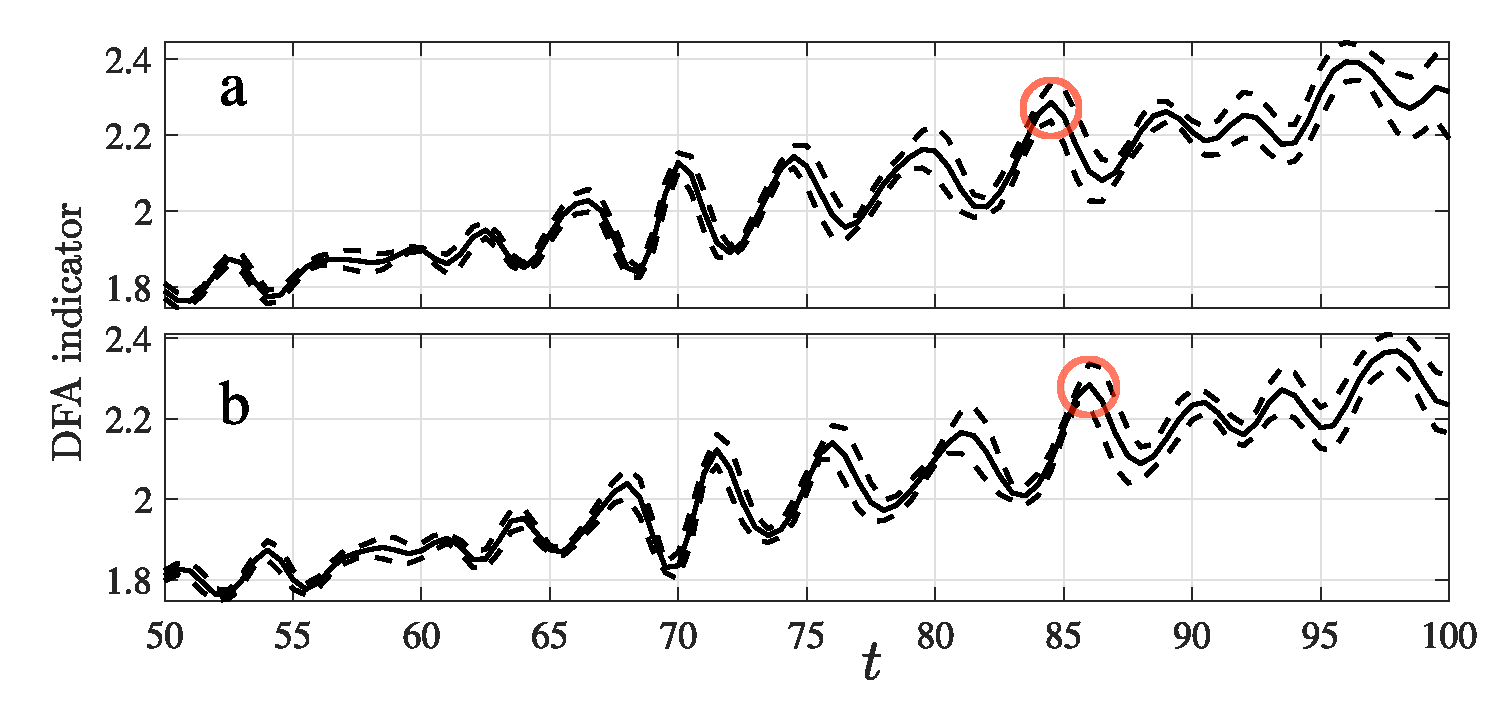
\includegraphics[width = 0.9\columnwidth]{AltEOFDFA_homoclinic}
	\caption{DFA indicator with a window of 100 points calculated for the one-dimensional time series obtained using the variance-based EOF technique (panel \textbf{a}) and the autocorrelation-based EOF technique (panel \textbf{b}) applied to the system described by equation~\ref{eqn:2D:Again-homoclinicSystem}, which experiences a bifurcation at $t=100$. In each panel the plot shows the mean over ten realisations of the dynamical system, with error bounds of one standard deviation. One example of a common feature is circled in red.
		\label{fig:2D:AltEOFDFA_homoclinic}}
\end{figure}

Having obtained the one-dimensional time series $X\underline{u}_\text{max}$ via this autocorrelation-based EOF technique, the DFA indicator is calculated with a window size of 100 points: figure~\ref{fig:2D:AltEOFDFA_homoclinic}b shows the result and, for comparison, the same process is also performed using the regular variance-based EOF technique (panel~\textbf{a}).  We see that there is little difference in the DFA indicator whichever EOF technique is used, the same features appear in both signals. However, the features appear earlier when the regular, variance-based EOF technique is used (panel~\textbf{a}). An example of a shared feature (a peak in the oscillating DFA indicator signal) is circled in red in figure~\ref{fig:2D:AltEOFDFA_homoclinic}: this feature occurs before $t=85$ in panel~\textbf{a} but slightly after $t=85$ in panel~\textbf{b}. This is not an artefact of the alternative EOF technique producing a lagged time series due to the lag in the autocorrelation, since only the lag-1 ACF is used and a single time step is of length $\Delta t=0.5$, whereas the apparent shift in the features of the DFA indicator signal is $\approx 1.5$. Rather, this is simply due to the different projection used to obtain the one-dimensional time series to which the DFA indicator is applied. 

To investigate the alternative EOF technique further, we also apply it to the other two-variable dynamical systems described in section~\ref{sec:2D:MethodsApplied}: the system experiencing a Hopf bifurcation (equation~\ref{eqn:2D:HopfSystem_noise}), to which we refer as "system B"; and the Van der Pol oscillator (equation~\ref{eqn:2D:VDPSystemCoupled}), or "system C". The system described in equation~\ref{eqn:2D:Again-homoclinicSystem} is referred to as "system A". Each of the three systems is integrated 100 times and both EOF techniques are applied to each resulting two-variable time series. In each case we record the eigenvector onto which the system is projected to obtain the one-dimensional time series. A multivariate time series has, for this purpose, two vectors $v_V, v_A$, characterised by their angles $\theta_V, \theta_A\in (-\pi,\pi]$, associated with it, and onto which we may chose to project it. The vector $v_V$ is the unit vector which maximises the variance, as the vector $\underline{u}$ in equation~\ref{eqn:2D:maxVector_EOFreg}, used in the regular variance-based EOF technique. The vector $v_A$ is the unit vector which maximises the autocorrelation, used in the alternative autocorrelation-based EOF technique. These vectors, for the three dynamical systems, are represented graphically on the half-circle in figure~\ref{fig:2D:EOFeigenvectors_comparison}. We see that in all three systems there is little variability in the variance-maximising vector (displayed in blue) but the autocorrelation-maximising vector is more sensitive to differences between different realisations of the system. This effect is visible, in particular, in System A, which is the subject of the study with the DFA indicator in figure~\ref{fig:2D:AltEOFDFA_homoclinic}. For each realisation of each system the angle difference $|\theta_V-\theta_A|$ is calculated and the mean is found to be 0.510 ($29.2^\text{o}$) in system A; 0.184 ($10.6^\text{o}$) in system B; and 0.162 ($9.30^\text{o}$) in system C. That is, in all three systems, the vector $v_A$ is closer to $v_V$ than the perpendicular. Particularly in systems B and C there will be little observable difference between the two projected time series. 


\begin{figure}
	\centering
	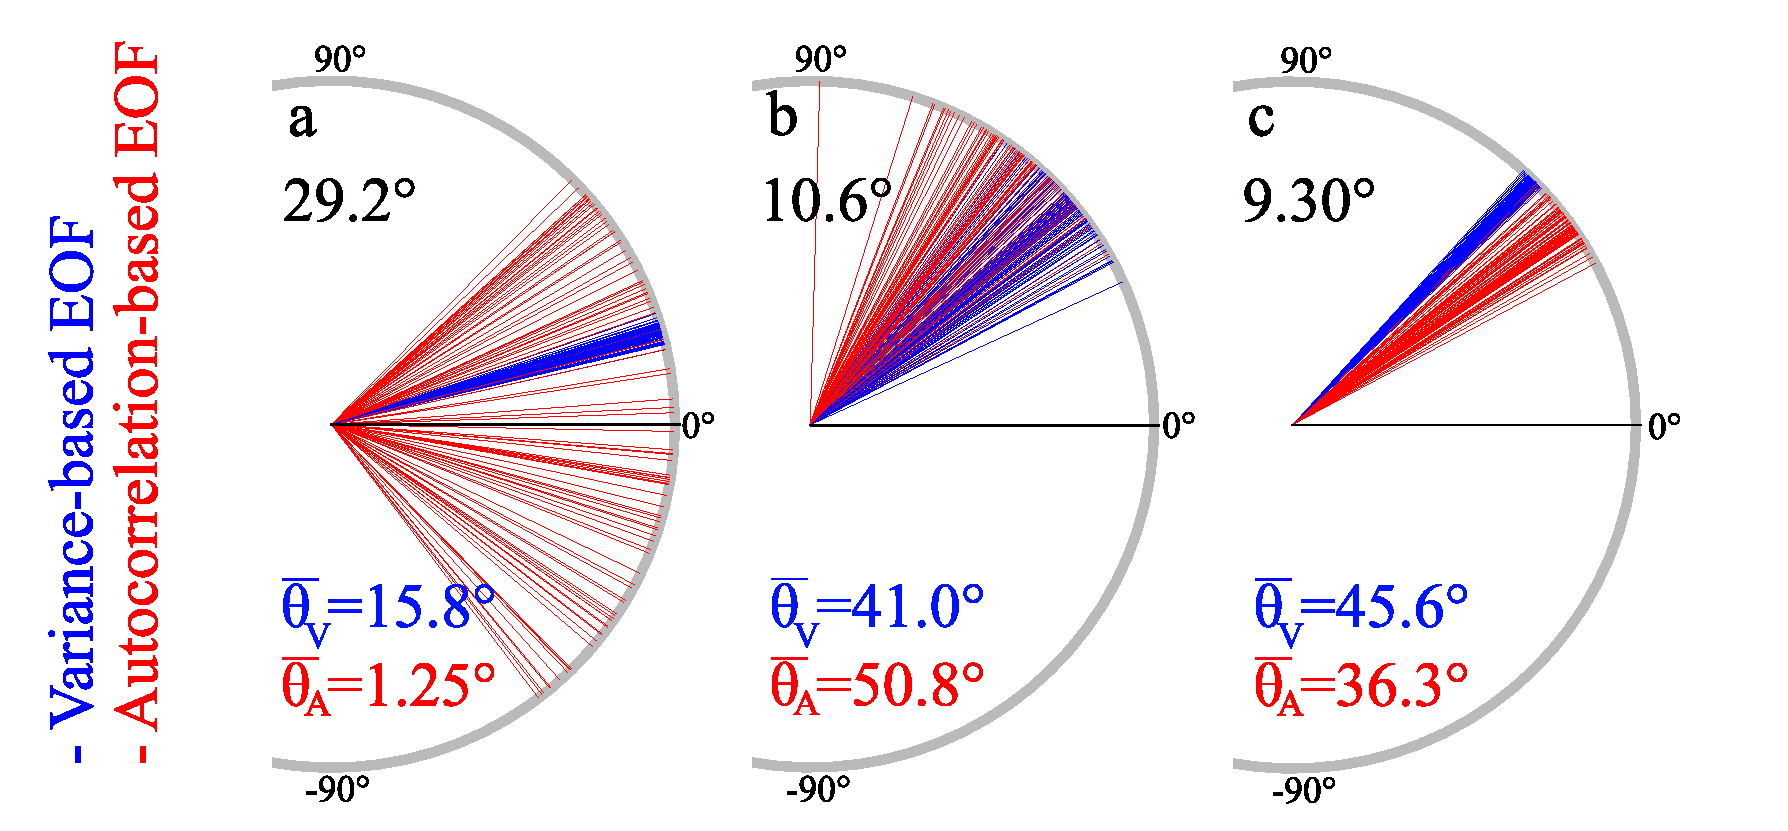
\includegraphics[width = 0.9\columnwidth]{EOFeigenvectors_comparison}
	\caption{Eigenvectors on the unit half-circle used to obtain the projection involved in the EOF technique (blue) and the alternative autocorrelation-based EOF technique (red) applied to 100 realisations of each dynamical system. Panel~\textbf{a}: system A (equation~\ref{eqn:2D:Again-homoclinicSystem}). Panel~\textbf{b}: system B (equation~\ref{eqn:2D:HopfSystem_noise}). Panel~\textbf{c}: system C (equation~\ref{eqn:2D:VDPSystemCoupled}). The mean difference (in degrees) in the angles, $\overline{|\theta_V-\theta_A|}$, is displayed in black font beneath the identifying panel letter. The mean angles $\overline{\theta_V}$ and $\overline{\theta_A}$ are displayed in their respective colours.
		\label{fig:2D:EOFeigenvectors_comparison}}
\end{figure}



\section{EWS in spatial data}
\label{sec:2D:ExtensionToGridded}

Besides techniques which allow one to detect or predict a tipping point in a multivariate system, we are also interested in dynamical systems evaluated over a data field. In a scenario where one has, for example, many time series associated with locations over a 2D field, one may reduce the dimension of the system using the EOF method to condense all of the available information. This can be refined if a specific region of interest is identified in advance: \citet{ludescher2013,ludescher2014} calculate the cross-covariance of a variable, at a specific time slice, between points inside the El Ni\~{n}o basin and points outside. In contrast, simply using the EOF method to reduce the dimension of such a system will not give specific spatial information such as the location of the tipping point or the direction of its progression in the case that a tipping at one location precipitates a tipping at other locations. However, one may also wish to use the spatial locations of the data, for example, to predict the location of the disturbance (a "hotspot") which is causing the tipping point: that is, locations where critical slowing down, and therefore loss of stability, is most apparent. \citet{bathiany2013p1} present a method to detect these hotspots: the method involves partitioning the locations ("elements") and, within each partition, discovering which elements contribute the most to the autocorrelation. This is done by combining the elements in different permutations, projecting onto the EOFs, and calculating the lag-1 autocorrelation of the resulting signal. Elements in each part are removed according to system-specific selection criteria and the remaining elements are re-partitioned. The process is repeated until only one partition remains, which is the slowing down hotspot where susceptibility to perturbations is large. The method is applied successfully to a highly idealised model of a vegetation cover. A similar method, also in the context of vegetation and aridity, is used by \citet{kefi2014early} who calculate the spatial correlation of the points across a two-dimensional field — the spatial variance and spatial frequency (where emerging spatially-repeating patterns are a symptom of the tipping) are also considered.

In this section we present a method to visualise the behaviour of the one-dimensional tipping point indicators introduced in chapter~\ref{chap:1D} evaluated at multiple locations, at a specific time slice, thus allowing one to observe locations, or hotspots, where a tipping point is likely to occur. 

\subsubsection{A 2D visualisation of indicator behaviour}

In figure \ref{fig:tikz-approachingfront} we illustrate an example of a propagating front over a 2D field. The time series $z_{xy}(t)$ is evaluated at each point $(x,y)$ on the field, and a tipping point occurs at the front (double line) which propagates from top-right to bottom-left. If we take the time series at points {\bf A} and {\bf B} and perform an EWS analysis, for example calculating the ACF1 indicator in a sliding window, we expect that the EWS will be stronger at point {\bf B} than at point {\bf A} because the tipping is closer (in time) to {\bf B}. Given some knowledge of the nature of the system one could conclude that the front is approaching from the right (from the positive $x$ direction) and, performing the analysis for more points in a grid over the field, one could determine more precisely the shape of the front and its direction. 

It will be difficult to visualise an ACF1 indicator series at every point on the grid (assuming the grid is larger than 3-by-3) in order to determine at which points the EWS is strongest. It is therefore useful to measure the increase in the indicator value at a specified point in time and to create a contour plot of this value over the grid.

\begin{figure}
	\centering
	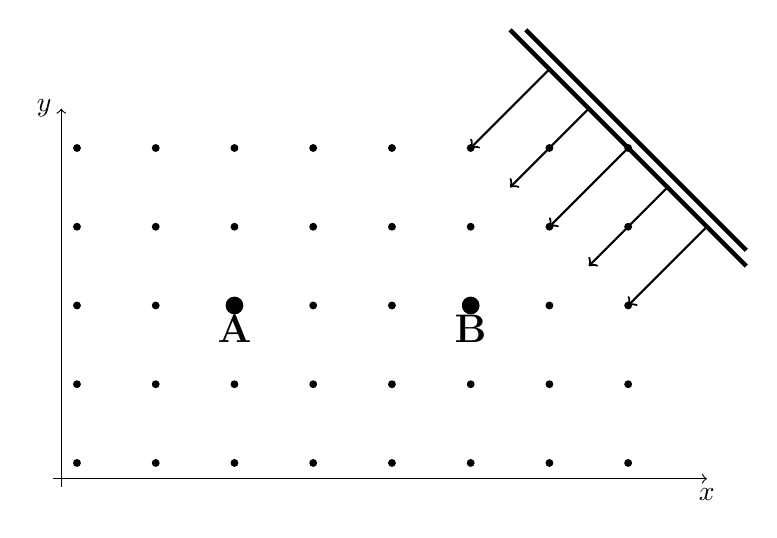
\begin{tikzpicture}
	\draw[->] (-2.3,-2.2) -- (6,-2.2) node[below] {$x$};
	\draw[->] (-2.2,-2.3) -- (-2.2,2.5) node[left] {$y$};
	
	\foreach \x in {-2,-1,...,5} {
		\foreach \y in {-2,-1,...,2} {
			\fill[color=black] (\x,\y) circle (0.05);
		}
	}
	
	\filldraw (0,0) circle (3pt) node[below] {\Large \bf A};
	\filldraw (3,0) circle (3pt) node[below] {\Large \bf B};
	
	\draw[-, ultra thick] (3.5, 3.5) -- (6.5,0.5);
	\draw[-, ultra thick] (3.7, 3.5) -- (6.5,0.7);
	\draw[->, thick] (4,3) -- (3,2);
	\draw[->, thick] (4.5,2.5) -- (3.5,1.5);
	\draw[->, thick] (5,2) -- (4,1);
	\draw[->, thick] (5.5,1.5) -- (4.5,0.5);
	\draw[->, thick] (6,1) -- (5,0);
	\end{tikzpicture}
	\caption{Propagating front. The time series $z_{xy}(t)$ is evaluated at each point on the field, and a tipping point occurs at the front (double line) which propagates from top-right to bottom-left. We expect that an EWS of the tipping point will be stronger at point {\bf B} than at point {\bf A} because the tipping is closer (in time) to {\bf B}.}
	\label{fig:tikz-approachingfront}
\end{figure}

As an example, we consider a system with a pitchfork bifurcation, which was used as an example in section \ref{sec:1D:indicatorComparison}. In this example, many similar dynamical systems are defined over the discrete $xy$ plane $\mathbb{Z}^2$, by the equation 
	\begin{equation}
		\frac{dz_{xy}}{dt} = -\frac{\partial}{\partial z_{xy}}\left(z_{xy}^4+\frac{\mu-x-y}{10}z_{xy}^2\right)+\sigma\eta_{xy},
	\label{eqn:propagatingPitchfork}
	\end{equation}
where the $\eta_{xy}$ are independently distributed Gaussian noise series. The line $y=-x+\mu$ defines the front: if $x+y<\mu$ the $z^2$ coefficient is positive and the system $z_{xy}(t)$ has a double-well generalised potential function; if $x+y\geq\mu$ then the system has a single-well potential. 

We create a 10-by-10 grid and integrate equation \ref{eqn:propagatingPitchfork} at each point $(x,y)$ from $t=0$ to $t=1000$ with time step $\Delta t = 0.05$. Parameter $\mu$ is made to decrease linearly at each time step so that at $t=0$, $\mu = 20$ and at $t=1000$, $\mu=10$. The series is sampled, after the integration, at intervals of one time unit to give a series of length 1000 points. For each time series $z_{xy}$, the ACF1 indicator is calculated in a sliding window of 100 points. In order to determine the location of the moving front at time $t$, one must determine whether the ACF1 indicator is increasing at each point $(x,y)$. We use the Mann-Kendall coefficient given by the equation
	\begin{equation}
		\label{eqn:2D:KendallCoef} 
		c(X) = \frac{2}{N(N-1)}\sum_{i=1}^{N-1}\sum_{j=i+1}^{N}\text{sign}(X_j-X_i),
	\end{equation}
for a time series $X$. This coefficient $c$ is calculated for each indicator series in the range $[t-100, t]$, thus showing whether the indicator series is increasing (positive coefficient) or decreasing (negative) in the 100-point window prior to time $t$. Figure~\ref{fig:2D:PitchforkContour-N10} shows the result when $t=1000$, that is, the time when $\mu=10$ and the pitchfork bifurcation is occurring in systems $z_{xy}$ on the line $x+y=10$. To the top-right of this line, the bifurcation has already occurred and the lag-1 ACF is decreasing (negative Mann-Kendall coefficient). To the bottom-left of this line, the systems have not yet bifurcated and the ACF1 indicator is increasing (positive Mann-Kendall coefficient) as an EWS of the approaching tipping point. As demonstrated in the simple application of the ACF1 indicator to the pitchfork bifurcating system in section \ref{sec:1D:indicatorComparison}, there is some variability in the indicator series and we cannot expect a completely smooth gradient to appear in the contour plot. However, the figure \ref{fig:2D:PitchforkContour-N10} does accurately represent the existence of a front. We note that a clear line between positive and negative appears to exist along the line $x+y =11$, because of the lag effect caused by the window size of 100 points used in the calculation of both the ACF1 indicator and the Mann-Kendall coefficient. This effect can be taken into account to conclude that the bifurcation is actually occurring some way in before the front apparent in the figure. The speed at which the front is advancing can be ascertained by taking snapshots of the system at intervals, that is, using a varying values of $t$ when calculating the Mann-Kendall coefficient in the preparation of the contour plot.
\begin{figure}
	\centering
	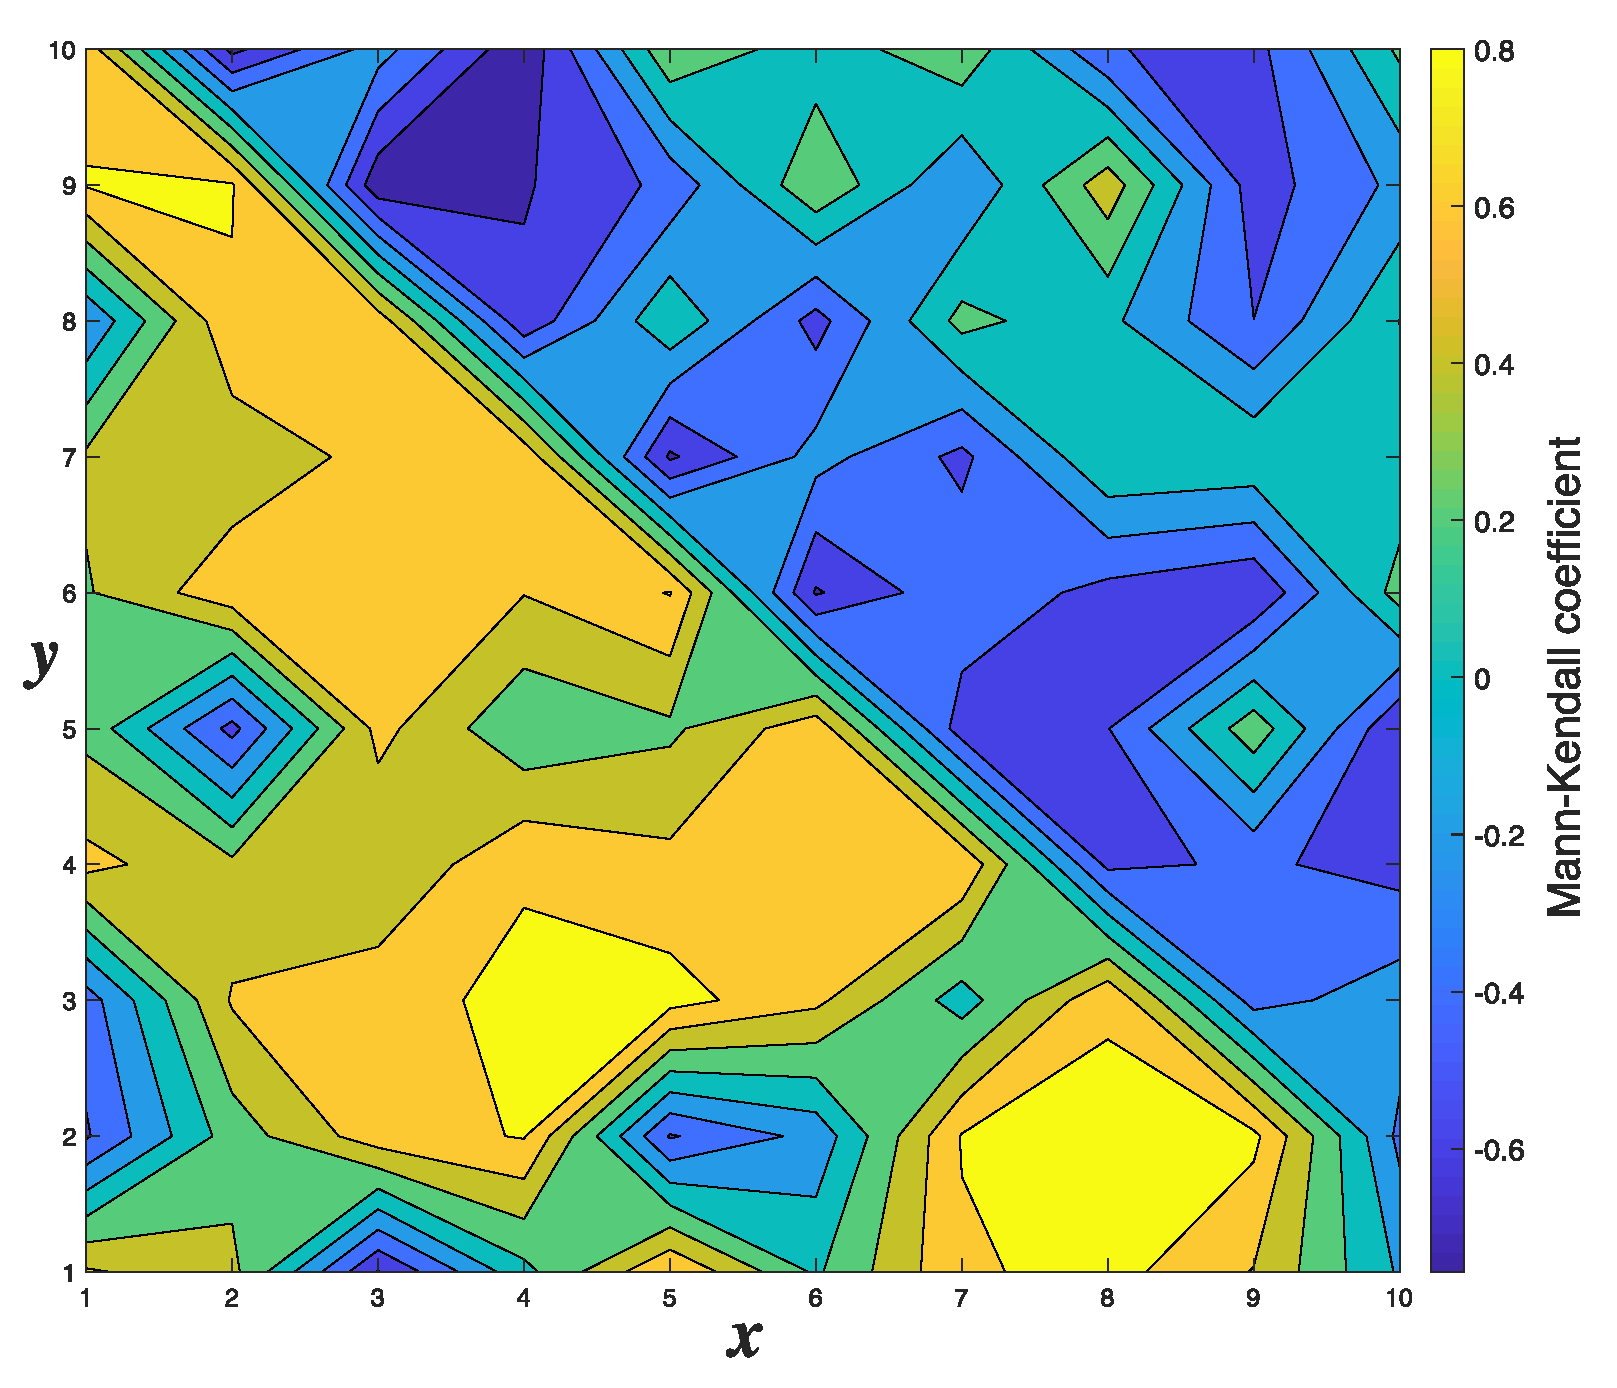
\includegraphics[width=0.9\textwidth]{PitchforkContour_N10}
	\caption{A 2D bifurcation caused by an approaching front. At each point $(x,y)$ a system is described by equation \ref{eqn:propagatingPitchfork} where the value of $\mu$ is decreasing. The figure shows the Mann-Kendall coefficient of the ACF1 indicator of the series when $\mu=10$, when the bifurcation is occurring at points on the line $y+x=10$. To the top-right of this line, the bifurcation has already occurred and the lag-1 ACF is decreasing (negative Mann-Kendall coefficient). To the bottom-left of this line, the systems have not yet bifurcated and the ACF1 indicator is increasing (positive Mann-Kendall coefficient) as an EWS of the tipping point.}
	\label{fig:2D:PitchforkContour-N10}
\end{figure}

If the experiment is repeated several times and the Mann-Kendall coefficient is calculated for the mean over all ACF1 indicator series at each point, the variability in the indicator will be smoothed and the line representing the front will be clearer. This may be necessary for systems where the indicator series contain greater variability, but impractical for applications where the experiment occurs only once.


\section{Discussion}
\label{sec:2D:discussion}

In this chapter we have presented techniques for detecting early warning signals in time series of more than one variable. The first technique, introduced by \citet{williamson2015}, reconstructs the eigenvalues of the system's Jacobian matrix using the relationship to the autocorrelation matrix. These eigenvalues are then used as indicators of a tipping point based on assumptions about the nature of the tipping. For example, a Hopf bifurcation in a two-variable system occurs when the Jacobian eigenvalues cross the imaginary axis, so calculating the behaviour of the imaginary part over time will provide a useful indicator which predicts a bifurcation as it approaches zero. The other technique presented uses EOFs to reduce the dimension of the system, before applying a familiar one-dimensional indicator to the resulting one-dimensional time series. We have applied both of these techniques to time series data from three known two-variable dynamical systems. In all cases the DFA indicator applied to the first EOF series provided a clear EWS in the mean. The ACF and PS indicators applied to the first EOF series did not give such a clear signal. The reconstructed Jacobian eigenvalues did provide an EWS in some cases, but it is necessary to know which eigenvalue to use.

We noted that the use of EOFs to reduce the dimension of a system, in an EWS context, assumes that the relevant signal will not be lost in the process. The EOF method projects a time series in such a way as to maximise the variance, which may not maximise the increase in the relevant tipping point indicator. We calculated the EOF scores analytically of a general linear dynamical system. We found that, except in contrived cases with very large variance in one variable, the EOF projection vector is similar to the direction in which the system diverges at a tipping point. We also devised an alternative EOF method which maximises the lag-1 autocorrelation of the projection rather than the variance. When applied to three dynamical systems we found that the projection vector was similar to that for the regular, variance-based, EOF method, but there was greater variability. 

In addition to this work, which concentrates on time series in several variables, with examples of two-variable systems, we have also studied dynamical systems defined over a discrete two-dimensional field. This type of data are particularly common in meteorology where data is collected at discrete locations over a geographic area (including the entire globe). We have proposed a simple method which may be used to visualise tipping point indicators over a field, and have applied this to an example based on a simple pitchfork bifurcation for which a reliable EWS can be obtained. This is a method to aid the visualisation of the tipping point indicator and it works as expected.

\subsubsection{Future work}

In the chapter we have used three dynamical systems as examples. It is always possible to apply the techniques presented here to more systems with different types of tipping. This work has been done with an aim of demonstrating the validity of using various techniques, rather than with a view to studying early warning signals in a comprehensive collection of dynamical systems. Indeed, when meteorological data is presented the type of tipping is often unknown: that is, it is not known whether or not the tipping is caused by, for example, a Hopf bifurcation in the underlying system. It is therefore useful to have a variety of techniques available that could be compared to infer the possible nature of the critical transition.

When calculating the EOF eigenvectors analytically for the general linear system, we did not calculate an error term by considering the variance in the system, we have only considered the mean. This does not appear to be possible without making further simplifications to the equations, but it may be possible to provide an estimate in future work.

It would be particularly interesting to use a general, simple system which is relevant to a meteorological event. In the next chapter, a specific model of a tropical cyclone is presented as a further test of the technique.



%!TEX root = ../thesis.tex

\chapter{Application of tipping point techniques to tropical cyclones}
\label{chap:cyclones}
\graphicspath{{Chap_Cyclones/Figs/}} % Define Graphics Path 
% References in this chapter have the identifier "TC"
% for Tropical Cyclones

In this chapter, we apply the techniques described previously to the real geophysical problem of providing an early warning signal for the approach of a moving tropical cyclone\footnote{A tropical cyclone is referred to as a ‘hurricane' when it occurs in the Atlantic Ocean and north-eastern Pacific Ocean  and a ‘typhoon' when in the north-western Pacific Ocean. In the south Pacific or Indian Ocean, comparable storms are referred to simply as ‘tropical cyclones' or ‘cyclones' \citep{NOAA_cyclones}. These naming conventions are not always abided by (e.g. Australian ‘hurricanes') and do not denote any differences in the physical properties of the storms other than geographic location.}. Typically, a steep drop in sea-level pressure is observed at the arrival of a cyclone, as shown in figure~\ref{fig:TC:SLP14}. {\Red{ This sudden, or `abrupt', change in the state of the system is not bifurcational in the sense that there are multiple stable system states, but it is nonetheless a tipping event in the general sense as defined by \cite{kuehn2011mathematical}, and we note that non-bifurcational tipping points (e.g. rate-induced tipping, noise-induced tipping, etc.) have previously been analysed using techniques similar to the ones used in this thesis \citep{livina2011,ashwin2012}. Similarly, there is a steep rise in wind speed at the same time (the same tipping point) and the early warning indicators we have developed may also be applied to the  wind speed time series beside the sea-level pressure.

The hypothesis is that it is possible to detect or predict this observed tipping point (the abrupt change in pressure and wind speed) using the same methods previously used to analyse examples of noise-induced, transitional or bifurcational tipping points. }}

A large tropical cyclone may extend hundreds of kilometres from its centre and a location on the future trajectory of such a storm experiences high winds several hours or days before the arrival of 200km/h winds. We expect, therefore, that the study of the weather variable at a fixed location will provide an early warning signal for the arrival of a tropical cyclone. The rise in wind speed itself acts as such a signal in a short (12 hour) period, but we are interested in the possibility that the tipping point techniques described in chapters~\ref{chap:1D} and~\ref{chap:2D} will provide an early warning signal when applied in this context.

{\Red{ We have no specific reason to expect that these EWS methods will be effective in this particular application but, in general, the sudden qualitative change in the system and the fact the a cyclone can be felt some way off make this a good candidate for investigation and experimentation.}}

In section~\ref{sec:TC:data} we give a description of the data used throughout this chapter, which has been obtained from the NOAA HURDAT2 database  \citep{HURDAT2} and the Met Office HadISD database \citep{HadISD}. In section~\ref{sec:TC:1Dtechniques} we apply the ACF1, DFA and PS indicators (see chapter~\ref{chap:1D}) to the sea-level pressure time series data from locations on the paths of fourteen tropical cyclones. In section~\ref{sec:TC:2Dtechniques} the same fourteen {\Red data sets} are used but both the sea-level pressure and the wind speed variables are considered and the techniques described in chapter~\ref{chap:2D} are applied to the two variables.

In section~\ref{sec:TC:field_data} we use sea-level pressure time series from several locations in a region through which a tropical cyclone passes. We apply the techniques introduced in section~\ref{sec:2D:ExtensionToGridded} to visualise the rise of a tipping point indicator over the area as the tropical cyclone approaches. This idea is further developed in section~\ref{sec:TC:Model} {\Red{where a model of the approaching cyclone is parametrised using the observed values of the tipping point indicators. The model is developed in order to verify the use of these indicators in the study of the tropical cyclone system.}}

\section{Description of data}
\label{sec:TC:data}

\subsection{The HURDAT2 database}
\label{subsec:TC:data:HURDAT}

During this study it was necessary to have track data of several Atlantic hurricanes, this was obtained from the NOAA national hurricane centre's HURDAT2 database \citep{landsea2013, HURDAT2}. This dataset is presented as a comma-delimited, text format with six-hourly information on the location, maximum winds, central pressure, and size of all known tropical cyclones and subtropical cyclones. We have only used the location data (given as latitude-longitude coordinates) and have not performed any additional processing of this data.


\subsection{The HadISD database}
\label{subsec:TC:data:HadISD}

For the purposes of our study we use sea-level pressure (SLP) and wind speed data from weather stations. These data are obtained from the HadISD 2017 data set \citep{HadISD_smith,HadISD_dunn12,HadISD_dunn14,HadISD_dunn16,HadISD} maintained by, and available from, the UK Met Office. The sea-level pressure and wind speed data provided by HadISD are raw data given at one-hour intervals, the Met Office applies a filter so that weather stations which provide very sparse data are disregarded \citep{HadISD_dunn12}, no other processing is applied.

The weather stations used in this study are selected for proximity to the landfall locations of tropical cyclones, and data are considered in a fifteen-day (360 hour) period before the time when the cyclone passes closest to the station. However, some of the weather stations provide very sparse data even after the Met Office's filtering, this is common at times when a tropical cyclone passes close to a station (presumably due to infrastructural damage). If fewer than 80\% of the time points have associated data, the time series is disregarded. Otherwise the data are interpolated linearly onto the entire hourly time series. We notice that weather stations on the United States mainland are more numerous than in other regions affected by tropical cyclones and also provide more consistent data. The examples used in this chapter are therefore dominated by Atlantic hurricanes making landfall in the USA.

In sections~\ref{sec:TC:1Dtechniques} and~\ref{sec:TC:2Dtechniques} we consider a single weather station associated with each cyclone, as close as possible to the landfall location, and we look at the single sea-level pressure and wind speed time series given at these stations. We consider 14 tropical cyclones selected for proximity of a weather station to the landfall location with reasonable data. Most of the cyclones selected, with the exceptions of Hurricane Jeanne and Hurricane Ernesto, are ranked category 4 or 5, using the SSHWS\footnote{The Saffir-Simpson hurricane wind scale (SSHWS) ranks cyclones based only on maximum one-minute sustained wind speeds. A cyclone with a wind speed of 209km/h or more is Category 4, with 251km/h or over is Category 5 \citep{NOAA_saffir}.}, at the time of landfall. These exceptions were included to broaden the scope of the study and because, although with a lower maximum wind speed, they exhibit a pronounced drop in pressure similar to the stronger cyclones. All 14 tropical cyclones are listed in table~\ref{tab:TC:14cyclones}, and the sea-level pressure time series are shown in figure~\ref{fig:TC:SLP14}. Many more than these 14 were considered initially, but in many cases a HadISD weather station did not exist close to the landfall location or, when it did, the data were sparse. 


\begin{table}
	\centering
	\begin{tabular}{ l  c  l  c  c  c }
		\hline
		\multirow{2}{*}{Name} & \multirow{2}{*}{Year} & \multirow{2}{*}{Location} & Min pressure & Max speed & Osc. amp. \\
		& & & (hPa) & (km/h) & (hPa) \\ 
		\hline \hline
		Flo     &  1990 & Shionomisaki (Japan)  & 890 & 270  & 0.91\\
		
		Andrew  &  1992 & Florida Keys (USA) & 922 & 280 & 1.09  \\

		Opal    &  1995 & Pensacola (USA) & 916 & 240 & 1.22\\
		
		Zeb	    &  1998 & Tuguegarao (Philippines)  & 900 & 285 & 1.15\\

		Floyd   &  1999 & Florida Keys (USA) & 921 & 250 & 1.15\\
		
		Charley &  2004 & Fort Myers (USA) & 941 & 240 & 1.17 \\
		
		Frances &  2004 & Florida Keys (USA) & 935 & 230 & 1.15 \\
		
		Jeanne  &  2004 & Florida Keys (USA) & 950 & 195 & 1.21 \\
		
		Katrina &  2005 & New Orleans (USA) & 902 & 280 & 1.24   \\
		
		Rita    &  2005 & Lake Charles (USA)  & 895 & 285 & 1.29  \\
		
		Ivan    &  2006 & Mobile (USA) & 910 & 270 & 1.18\\
		
		Ernesto &  2006 & Florida Keys (USA)  & 985 & 120 & 1.05\\
				
		Megi    &  2010 & Tuguegarao (Philippines) & 885 & 295 & 1.31  \\
		
		Hudhud  &  2014 & Vishakhapatnam (India)   & 950 & 260 & 1.29   \\
		\hline
	\end{tabular}
	\caption{The dates and locations of each of the 14 tropical cyclones considered. The "Location" column data is the identifying location recorded on the HadISD database for the weather station used in this study. The "Max speed" column gives the highest one-minute sustained wind speed (a value over 209~km/h puts the cyclone into SSHWS category 4 or higher). The data in the pressure and wind speed columns is not used in this study and is given for information only. It is obtained from the NOAA archive \citep{NOAA_archive} in the cases of the Atlantic hurricanes (those in the USA), and from \protect\url{www.wikipedia.org} otherwise. The column "Osc. amp." gives the amplitudes of the 12-hourly oscillations in the sea level pressure data from that weather station but in a period 50 to 15 days before the cyclone event (this is discussed in section~\ref{subsec:TC:data:oscillations}).}
	\label{tab:TC:14cyclones}
\end{table}

\begin{figure}
\centering
	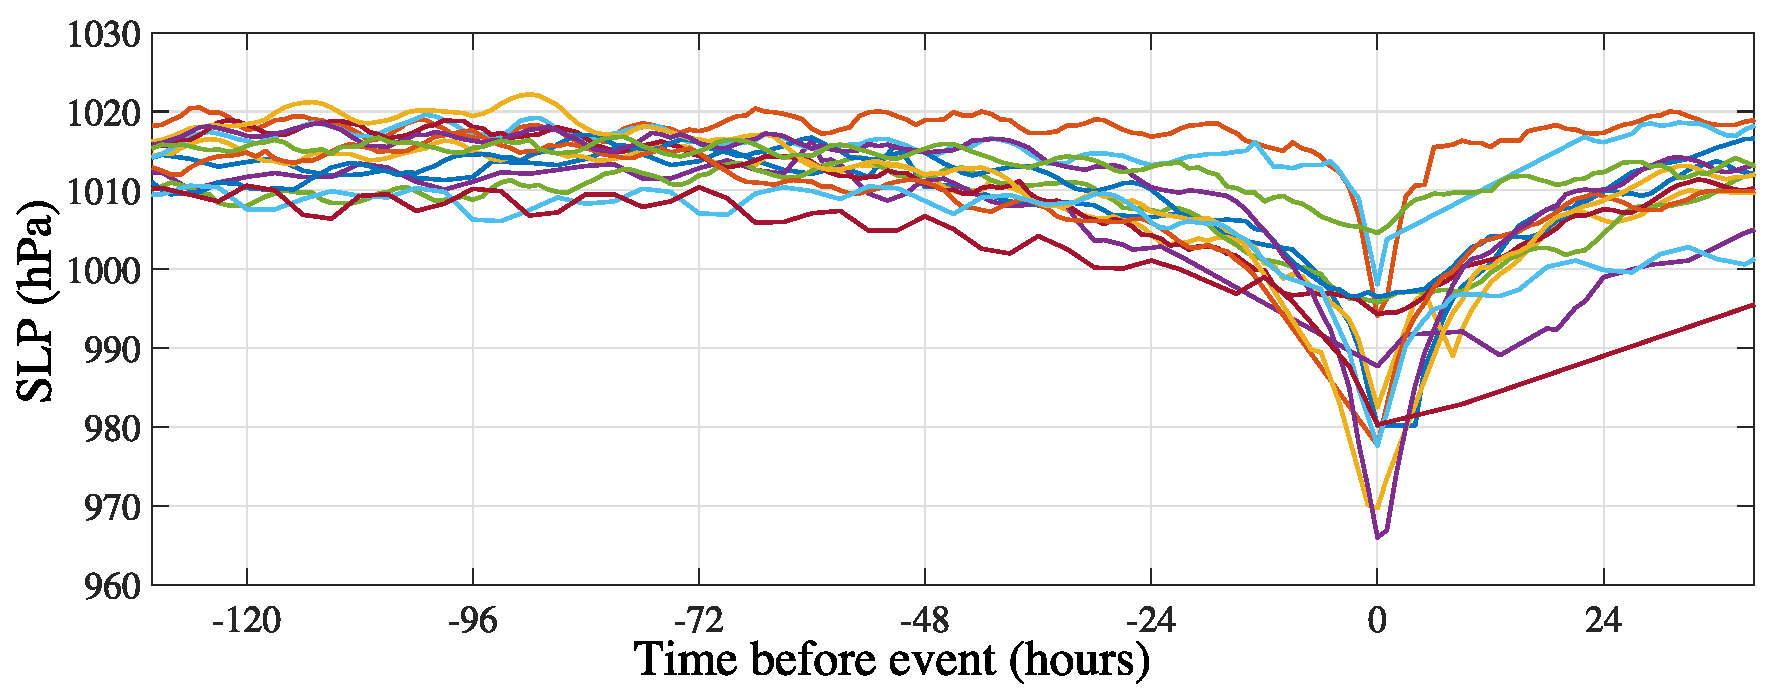
\includegraphics[width = 0.9\textwidth]{PlotSLP14}
	\caption{Sea-level pressure time series for the fourteen tropical cyclones selected in table~\ref{tab:TC:14cyclones}. The minimum point in the data is presumed to be the point closest to the time at which the cyclone was closest to the station and is set as time zero.
		\label{fig:TC:SLP14}}
\end{figure}

In section~\ref{sec:TC:field_data} we consider the data given by several weather stations in a region surrounding the path of the cyclone. Because of better availability of data, all the cyclones in this case are Atlantic hurricanes making landfall on the Caribbean or Florida coastlines of the United States. The eight hurricanes considered are listed in table \ref{tab:TC:9hurricanes}, Hurricane Andrew appears twice (labelled Andrew 1 and Andrew 2) because it made landfall twice: over Florida and then, two days later, over Louisiana. We therefore have a total of nine hurricanes. Again, we use the HadISD 2017 data set \citep{HadISD_dunn12,HadISD_dunn14,HadISD_dunn16,HadISD_smith}. {\Red{We take data from stations within 200~km of the landfall of each hurricane and a region is formed by the minimal rectangle containing all of the weather stations used, which amounts to $65$ stations at separate locations. In some cases the stations did not provide `good' time series data and so the number used in the analysis of each hurricane is lower than $65$ in each case and is between $21$ and $48$ stations depending on the hurricane (see column ``\# stations'' in table~\ref{tab:TC:9hurricanes})}}. We use the HURDAT2 track data \citep{landsea2013} (see section~\ref{subsec:TC:data:HURDAT}) in each case to find the point at which the hurricane entered this region. 

\begin{table}
	\centering
	\begin{tabular}{ l  l  l  c c }
		\hline
		Name & Date & Region & Entry point & \# stations\\
		\hline \hline
		Andrew 1 &  24 August 1992 &      Florida     &   [25.4N,    -79.0E] &21\\

		Andrew 2 &  26 August 1992 &      Louisiana  &  [29.8N,  -91.6E]&34\\

		Katrina &   29 August 2005 &     Louisiana &   [29.3N,   -89.6E]&45\\

		Wilma &     24 October 2005 &   Florida     &   [25.3N,    -82.7E]&34\\

		Gustav &  1 September 2008 &   Louisiana & [29.3N,    -90.8E]&46\\

		Matthew &  7 October 2016 & Florida     & [26.7N,    -79.0E]&32\\

		Harvey  &  25 August 2017 &      Texas       &  [25.2N,    -94.6E]&29\\

		Irma &        10 September 2017 & Florida    &  [24.5N,    -81.5E]&34\\

		Nate &       8 October 2017 &    Louisiana &   [29.3N,   -89.2E]&48\\
		\hline
	\end{tabular}
	\caption{\Red{ The dates and locations of each of the nine hurricanes selected. The entry point column gives the coordinates at which each hurricane entered the region, calculated using the HURDAT2 track data. Hurricane Andrew appears twice (labeled Andrew 1 and Andrew 2) because it made landfall twice: over Florida and then, two days later, over Louisiana. The column `\# stations' gives the number of weather stations in the region from which data was used when analysing each hurricane. }}\label{tab:TC:9hurricanes}
	% for i = 1:9
	% disp([SuperStruct(i).name,': ',num2str(size(SuperStruct(i).allValues,1))])
	% end
\end{table}

\subsection{Filtering sea-level pressure oscillations}
\label{subsec:TC:data:oscillations}

Upon inspection of the sea-level pressure data we see that there is a small, regular oscillation superimposed on the longer term fluctuations, figure~\ref{fig:TC:osc_and_powerspectrum}a shows this phenomenon at the Florida Keys station prior to Hurricane Andrew. An inspection of the power spectrum shows that the oscillations have a period of 12 hours (see figure~\ref{fig:TC:osc_and_powerspectrum}b) and are due to the daily tidal cycle. We calculate the mean amplitude of the oscillations over a given time period by subtracting the minimum pressure from the maximum pressure in a 12-hour sliding window and taking the mean. The "Osc. amp." column in table~\ref{tab:TC:14cyclones} records the mean amplitude found in the sea-level pressure data at each station in a period from 50 days before to 15 days before each of the tropical cyclone events: despite being recorded at different locations around the world over a period of 20 years, there is little variation in the size of these oscillations (mean: 1.17, variance: 0.011, range: $[0.91, 1.31]$). Because of this regularity, the possibility of removing the oscillations was proposed, and the effects of doing this were studied in the context of early warning signals, that is, we asked how the autocorrelation of the time series would be affected by the removal of the oscillations. 
	\begin{figure}
		\centering
		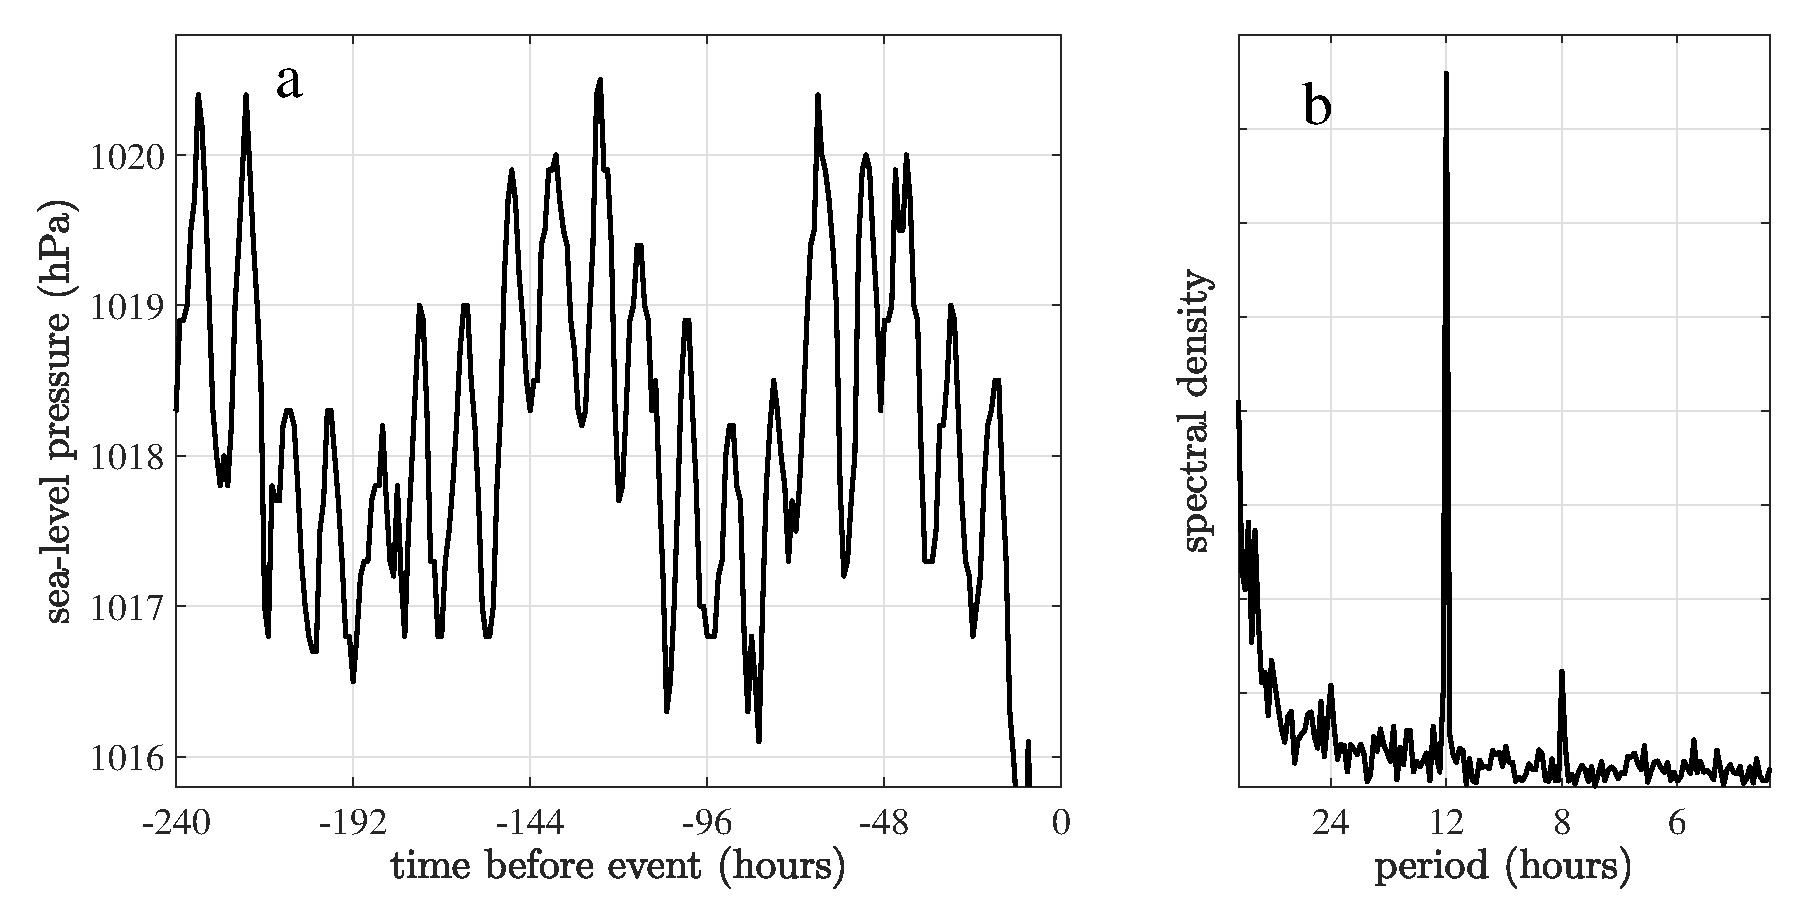
\includegraphics[width = 0.9\textwidth]{osc_and_powerspectrum}
		\caption{Sea-level pressure periodic oscillations. Panel \textbf{a}: A 240 hour segment of the sea-level pressure data preceding the Hurricane Andrew event, we note the 12-hour oscillations on the longer term fluctuations. Panel \textbf{b}: The periodogram obtained from a 35 day segment of the same time series (between 15 and 50 days before the event), we note the spike at 12 hours.
			\label{fig:TC:osc_and_powerspectrum}}
	\end{figure}
Two approaches were employed. First, a filtering approach where, given a time series $[Z]_k$ a deseasonalised series $[Z_\textrm{D}]_k$ is created according to the formula
	\begin{equation}
		Z_\textrm{D}(k) = Z(k)-\underset{_{i = k~\textrm{mod}12}}{\textrm{mean}}\left({Z(i)}\right).
		\label{eqn:TC:deseasonalise}
	\end{equation}
The other approach is to subtract a sine wave with 12 hour period, that is, a new series $[Z_\textrm{S}]_k$ is given according to
	\begin{equation}
		Z_\textrm{S}(k) = Z(k) - A\sin\left(\frac{2\pi}{12}(k - \phi)\right)
		\label{eqn:TC:subtractsinewave}
	\end{equation}
where $A$ is the mean amplitude found over the entire series, as described above, and $\phi$ is required to align the series $Z$ with the sine wave. In practice, the phase $\phi$ was found in each case by minimising the variance of $Z_\textrm{S}$ over values of $\phi\in[0,12)$. 

{\Red{
Both of these approaches are applied to pressure data from the Florida Keys station in the period of 50 to 15 days before the appearance of Hurricane Andrew, and for both of the new series, as well as the original raw series, the ACF1, DFA and PS indicators are calculated and the results are shown in figure~\ref{fig:TC:removeOsc}. In the calculation of the indicators, the sliding window used is $90$~points for ACF1, $90$~points for DFA, and $102$~points for PS; these window sizes are chosen according to the sensitivity analysis (see section~\ref{subsec:TC:1D_SA}) and are consistent with those used throughout this chapter.

We note that both methods of removing oscillations give almost identical results, both qualitatively and when considering the autocorrelation of the resulting series.

The effect on the ACF1 indicator is, effectively, of smoothing out the larger fluctuations but it does not appear to change the general shape of the indicator series (that is, longer scale increases or decreases). The same is true of the DFA and PS indicators, although in the case of the DFA indicator there is apparently some extra detail visible when using the filtered series (red and blue lines) which is not visible when using the original, oscillating data: specifically, there appears an increase in the DFA indicator (both red and blue lines) starting after $\m 600$ hours, which cannot be seen in the grey line. 

We suggest it may be beneficial, especially when using the DFA indicator, to first filter the tidal oscillations in the sea-level pressure data before attempting to produce an early warning signal. However, it is not apparently important whether the deseasonalising approach or sine-wave approach is used. For the remainder of this chapter, the deseasonalising approach (see equation~\ref{eqn:TC:deseasonalise}) is used whenever oscillations are removed from data in this way.



%For this reason the 12-hour oscillations in pressure were not removed in further analysis of the tropical cyclone data.
}}

\begin{figure}
	\centering
	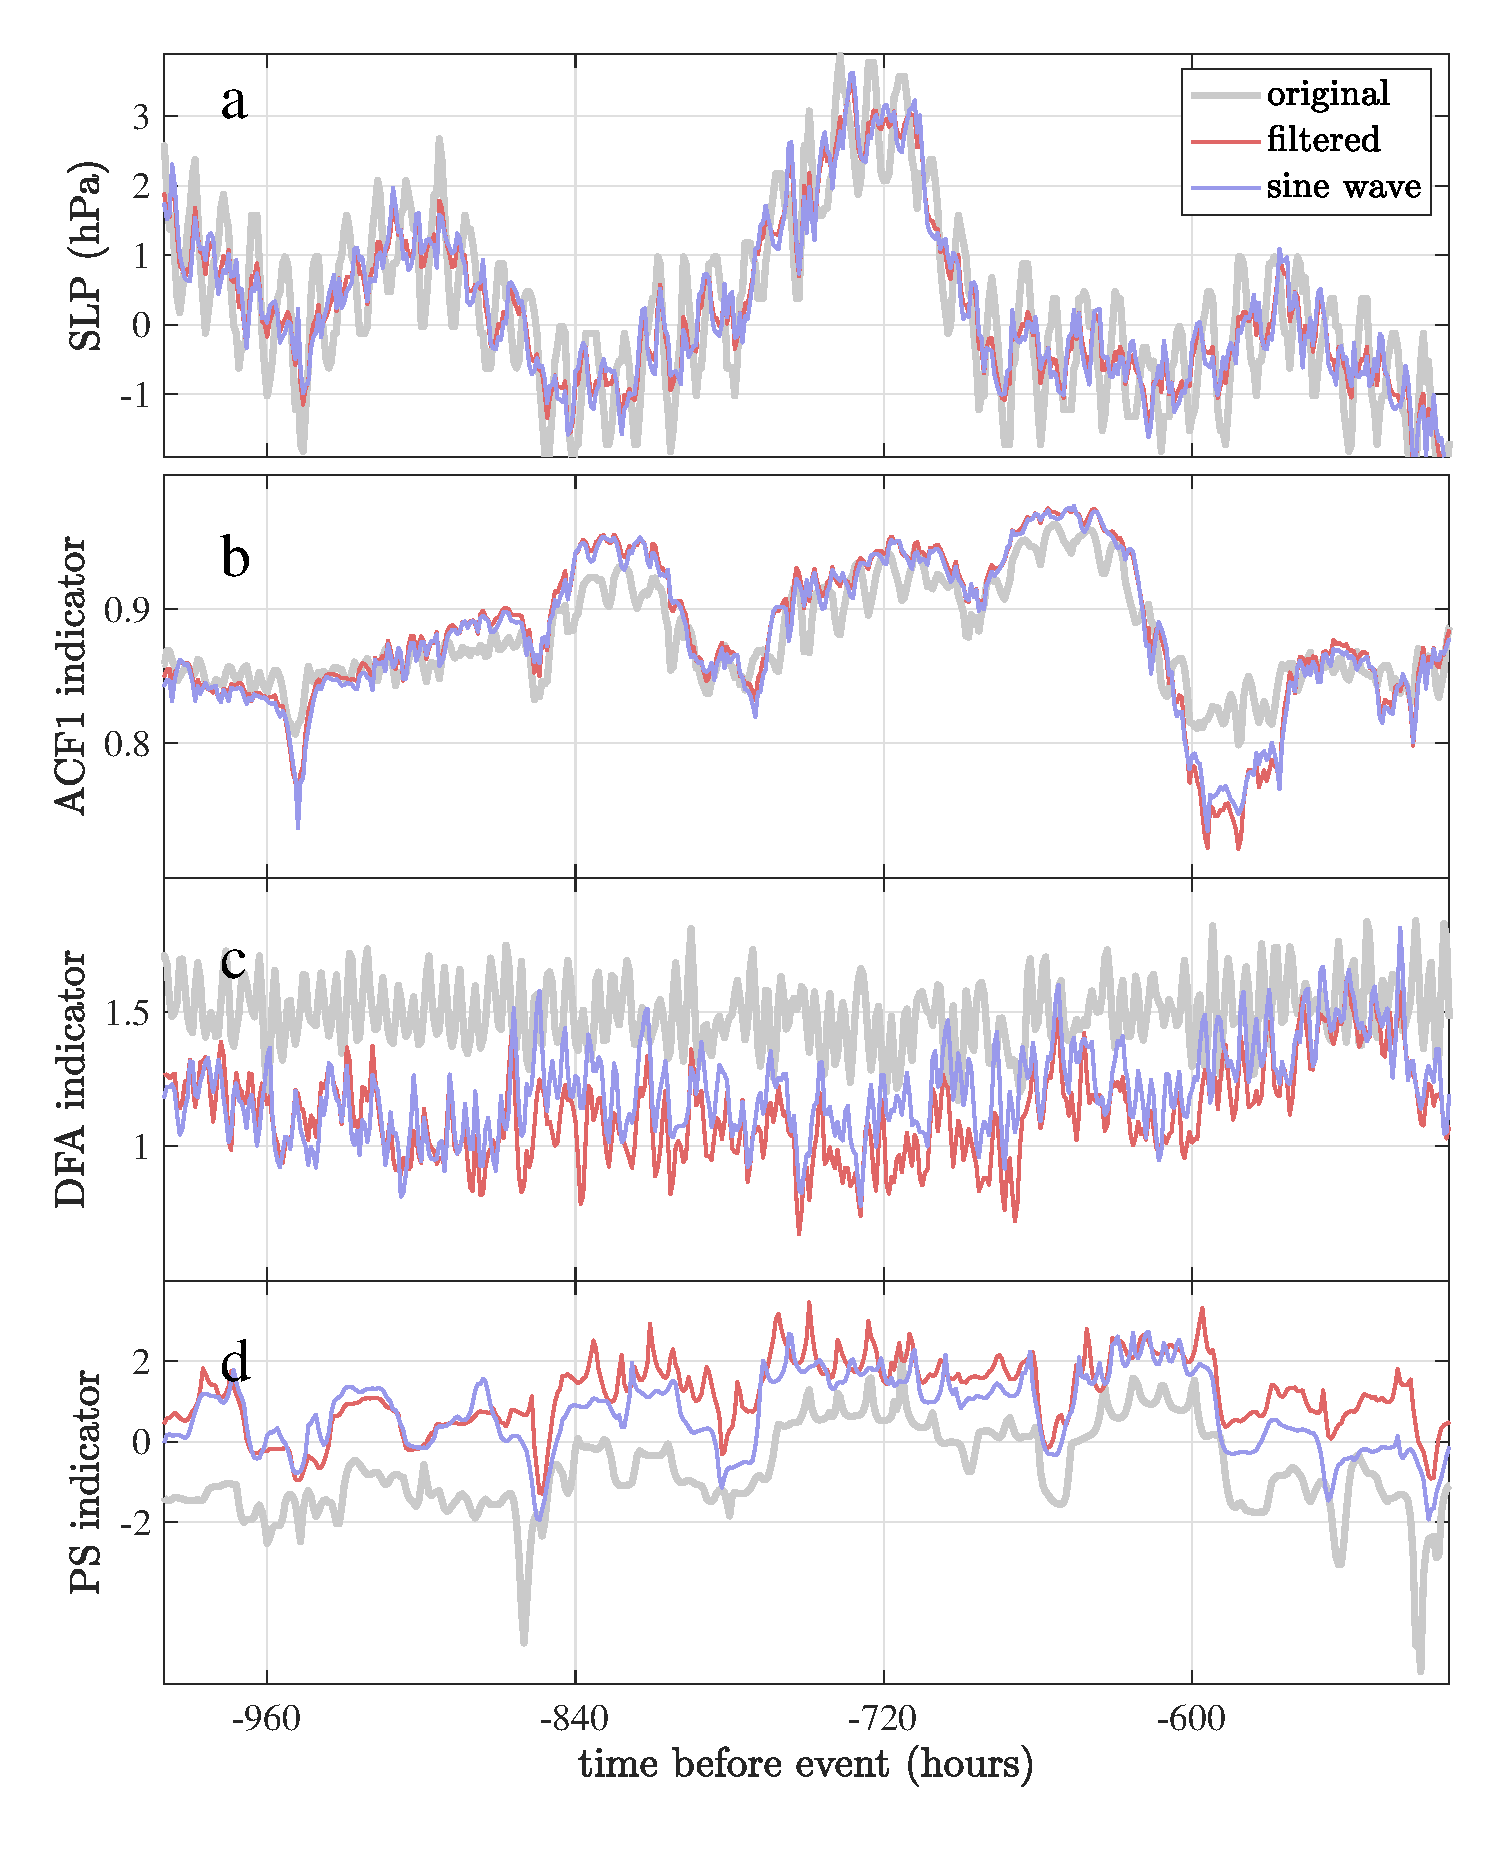
\includegraphics[width = 0.9\columnwidth]{removeOsc_all3}
	\caption{\Red{Sea-level pressure deviation from the mean at the Florida Keys station in a period from 15 to 50 days before Hurricane Andrew. Three time series are considered: the original raw data (grey line); the same data with oscillations removed by filtering (red, see equation~\ref{eqn:TC:deseasonalise}); and the data with oscillations removed by subtracting a sine wave (blue, see equation~\ref{eqn:TC:subtractsinewave}). Panel \textbf{a} shows the sea-level pressure deviation from the mean whilst panels \textbf{b}, \textbf{c} and \textbf{d} show the ACF1, DFA and PS indicators (respectively) of the three series.}}
	\label{fig:TC:removeOsc}
\end{figure}


\subsection{Evidence of scaling in the sea level pressure series}
\label{subsec:TC:evidenceOfScaling}

{\Red{
In figure~\ref{fig:TC:osc_and_powerspectrum} (page~\pageref{fig:TC:osc_and_powerspectrum}) we presented the periodogram of the sea level pressure time series from the weather station chosen for its proximity to the landfall location of Hurricane Andrew. Now, in figure~\ref{fig:TC:PS_loglog_RO12}, we present the periodograms from all fourteen stations chosen for each of the fourteen tropical cyclones detailed in table~\ref{tab:TC:14cyclones}. In each case we use a time series of length 2400 hours which terminates 96 hours before the cyclone event, so that this is not included. Additionally, the spike at the 12-hour period has been removed by removing the oscillations, as discussed in the previous section. The periodograms are plotted on a log-log scale so that a linear trend, which is evidence of power-law scaling, may be apparent. The periodograms are plotted in the frequency range $\m2\leq\log f\leq\m1$ since this is the range used for the estimation of the PS exponent.

We note that in some cases there appears to be definite power-law scaling, such as in the example of Flo (top left panel), whereas other periodograms appear to contain crossovers in the given frequency range, or show little evidence of any correlation. In general the periodograms show a negative linear gradient as expected in correlated (red noise) signals. 

As we have remarked in section~\ref{subsec:1D:Exponents_as_EWS:nopowerlawsacaling}, the estimation of the PS exponent for use as the PS indicator does not assume power-law scaling and merely seeks to detect a `reddening' of the signal, which is present even in systems such as the AR(1) process which do not exhibit true power-law scaling in the asymptotic. 
}}

\begin{landscape}
	\begin{figure}
		\centering
		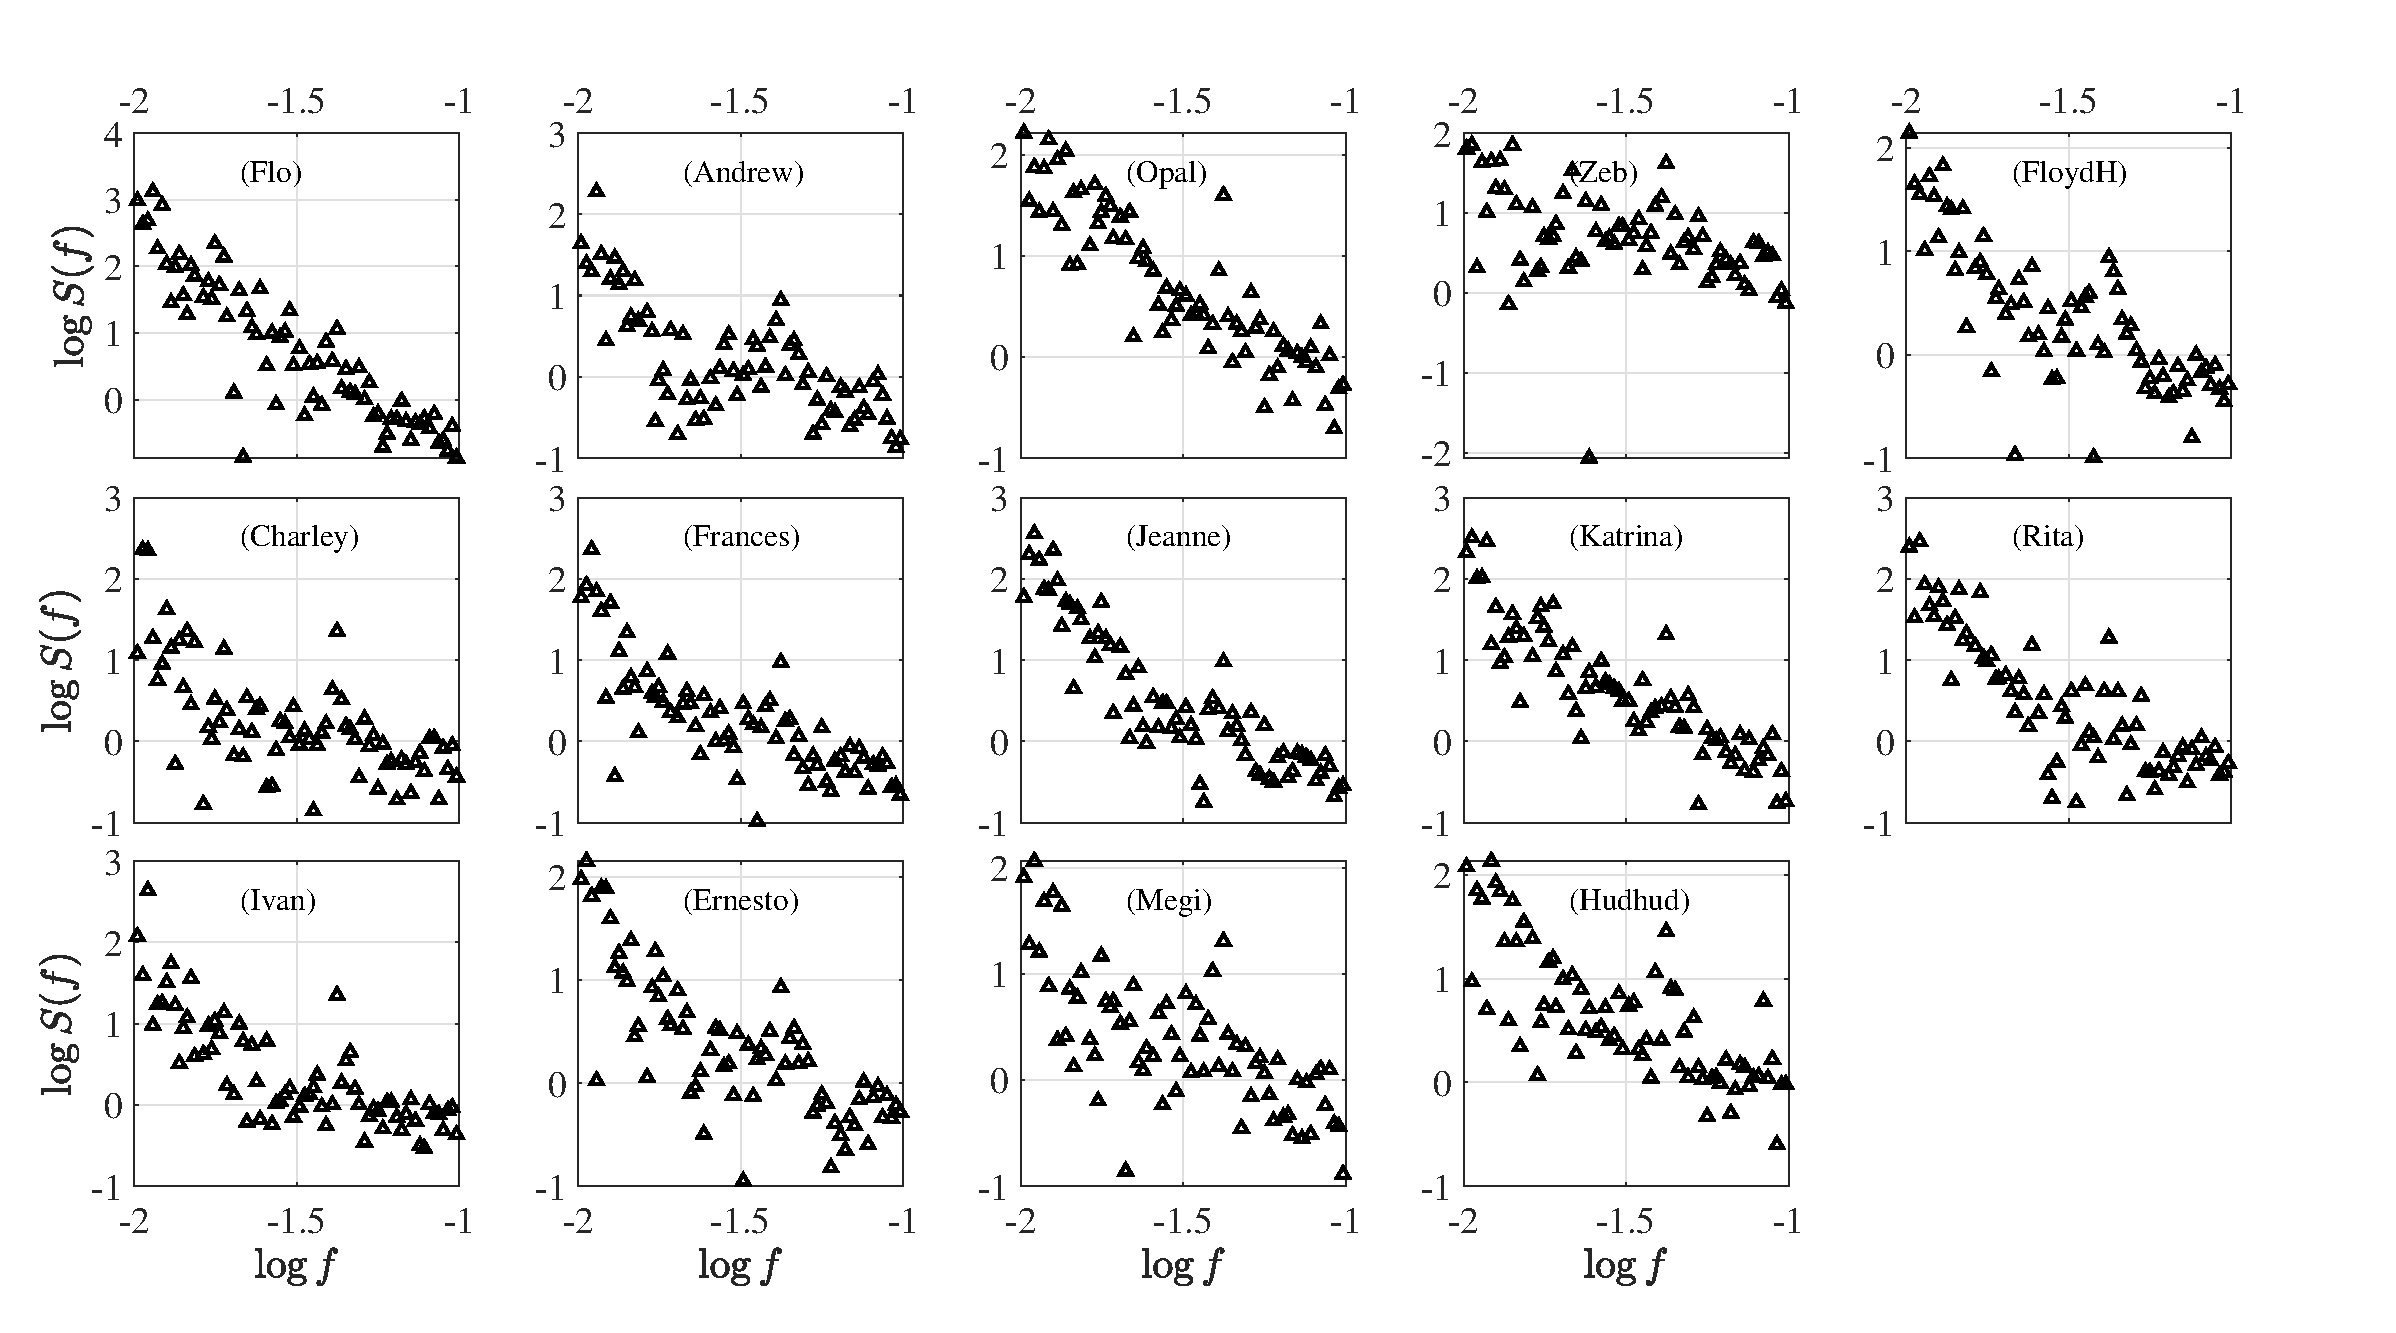
\includegraphics[width=\linewidth,keepaspectratio]{PS_loglog_RO12}
		\caption{\Red{The periodogram for each of the sea level pressure series from weather stations chosen for each of the fourteen tropical cyclones detailed in table~\ref{tab:TC:14cyclones}. In each case we use a time series of length 2400 hours which terminates 96 hours before the cyclone event, and the 12-hour period oscillations have been removed.
		}}
		\label{fig:TC:PS_loglog_RO12}
	\end{figure}
\end{landscape}


\section{Application of one-dimensional tipping point techniques}
\label{sec:TC:1Dtechniques}

In this section we consider the time series of the sea-level pressure variable at a fixed location in the time immediately before the arrival of a tropical cyclone in that location. We use the fourteen tropical cyclones that are detailed in table~\ref{tab:TC:14cyclones} (see section~\ref{subsec:TC:data:HadISD}). 

In the case of each of the fourteen cyclones, the sea-level pressure time series is centred on the minimum pressure value which is labelled $t=0$. This cannot be called analogous to the bifurcation point in the pitchfork bifurcation example of chapter~\ref{chap:1D}  (figure~\ref{fig:1D:pitchforkEWS}, page~\pageref{fig:1D:pitchforkEWS}) but is a common feature of all time series which is convenient to use for the purpose of comparison. {\Red{The results presented in this section have previously been published in \cite{prettyman2018}.}}

\subsection{Method}
\label{subsec:TC:1Dmethod}

The same methods are applied to the sea-level pressure time series here as are applied to the model examples in section~\ref{sec:1D:indicatorComparison}. The ACF1, DFA and PS indicators {\Red (definitions \ref{def:1D:indicator:ACF1}, \ref{def:1D:indicator:DFA} and \ref{def:1D:indicator:PS} respectively, see section~\ref{sec:1D:Exponents_as_EWS}, page~\pageref{sec:1D:Exponents_as_EWS}) } are applied to the times series with a sliding window of approximately 100 points, equivalent to 100 hours in this data. The exact window sizes used, for each indicator, are: ACF1: $90$~points; DFA: $90$~points; PS: $102$~points. These values are determined by the sensitivity analysis which will be explained in section~\ref{subsec:TC:1D_SA}. Each of the three indicator series is calculated for each of the fourteen time series and then the mean over these fourteen series is calculated.

\begin{figure}
	\centering
	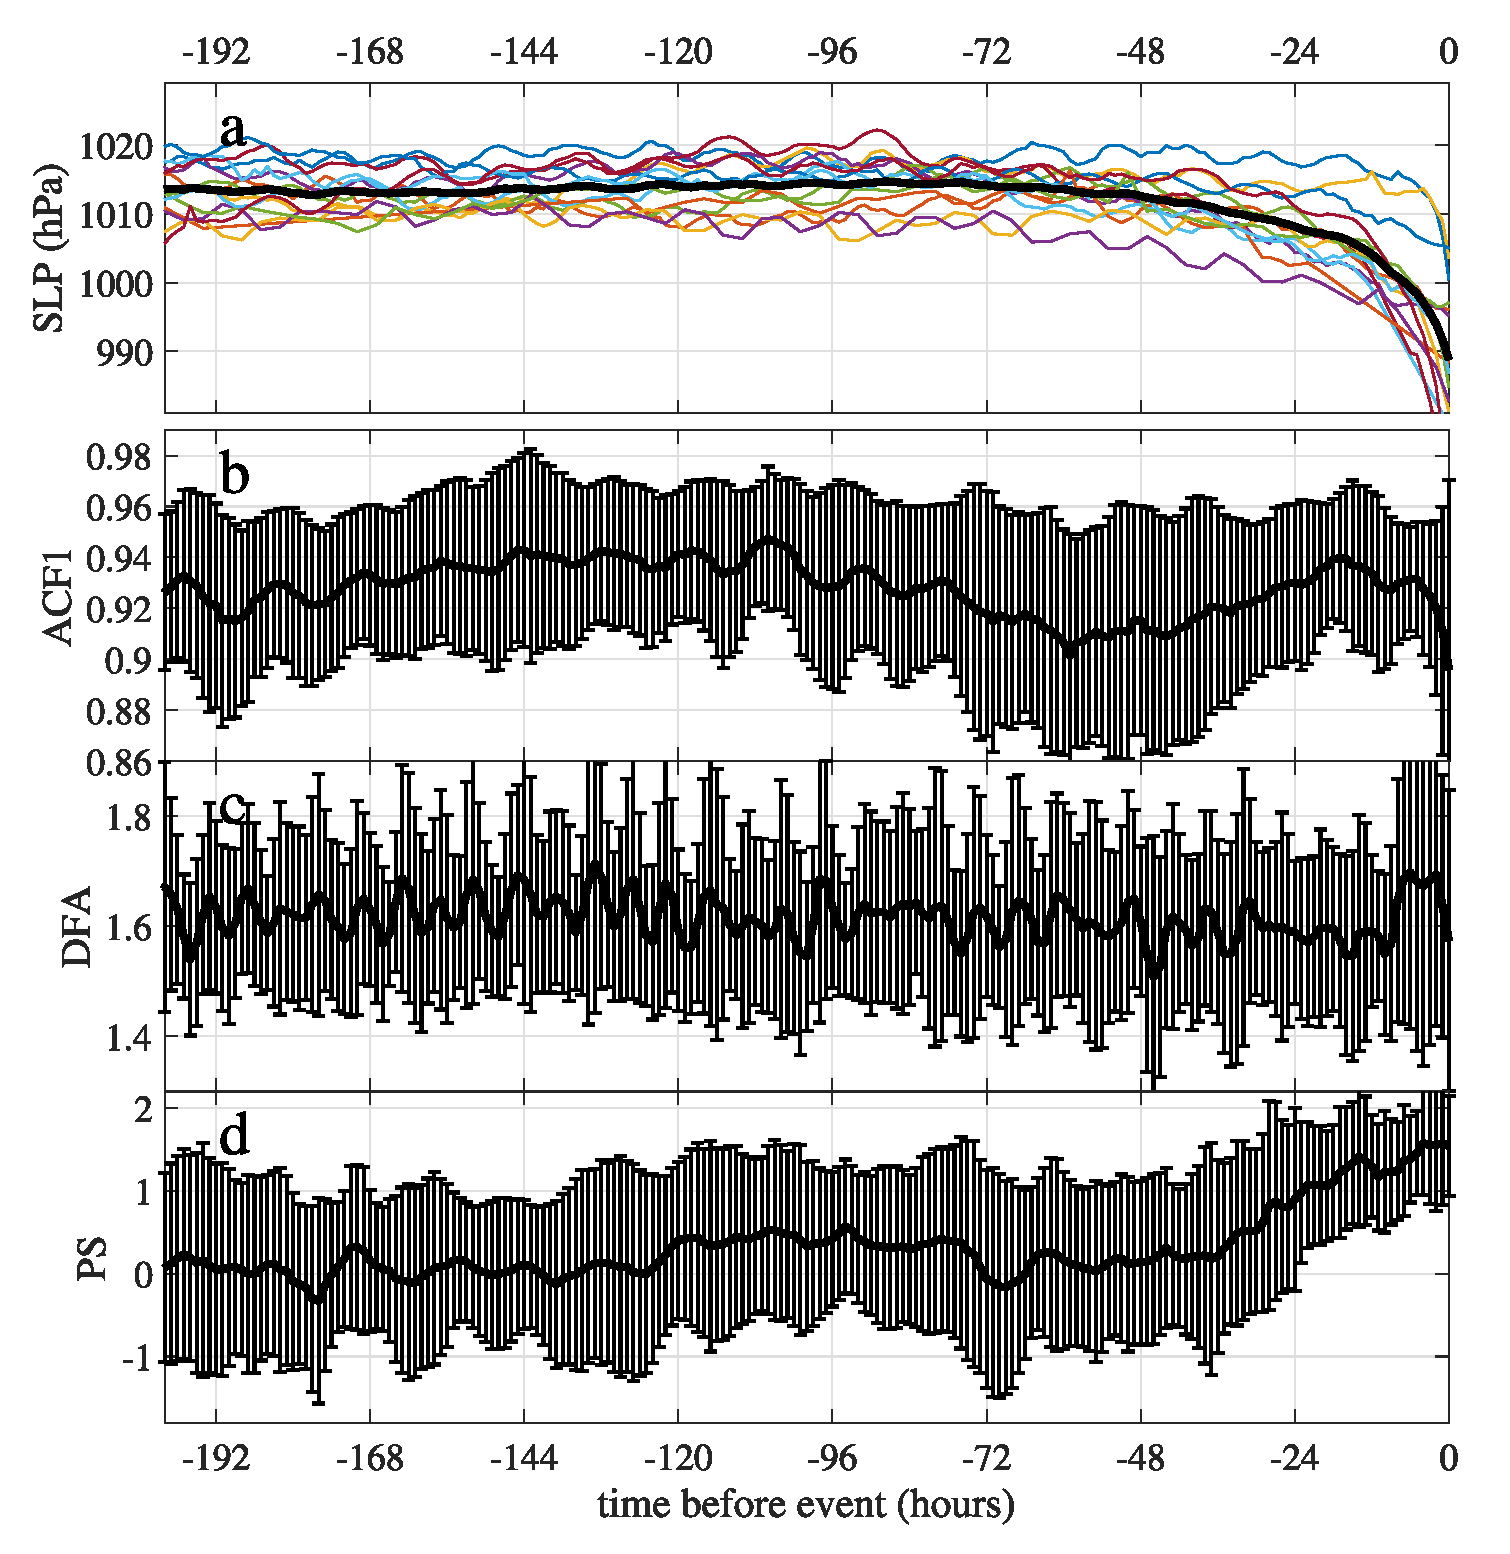
\includegraphics[width = 0.9\textwidth]{indicators14_slp}
	\caption{ACF1, DFA and PS indicators applied to sea-level pressure data. Panel {\bf a}: Data from the 14 tropical cyclones, mean shown in black. Panels {\bf b}, {\bf c}, {\bf d}: The mean ACF1, DFA and PS indicators, with error bars of 1 standard deviation. The ACF1 indicator does not provide a clear EWS in this case. The DFA indicator shows a small, sudden increase just before the event. The PS indicator begins to rise around 48 hours before the cyclone event. \label{fig:TC:1DindicatorsSLP}}
\end{figure}

\subsection{Results}
\label{subsec:TC:1Dresults}


Figure~\ref{fig:TC:1DindicatorsSLP} shows the fourteen sea-level pressure time series centred at the point of minimum pressure (panel \textbf{a}) and the mean of the three indicator series (ACF1, DFA and PS indicators in panels \textbf{a}, \textbf{b} and \textbf{c}). The mean indicator series are shown with error bars of one standard deviation. 

We note that the ACF1 indicator is consistently high (greater than $0.9$) over the entire series and does not apparently rise as a precursor of the cyclone event. The mean of the DFA indicator increases within the time period that the drop in pressure is obvious in the time series (24 hours before the event), and so the increase cannot be said to be an early warning signal. The PS indicator, however, does show an increasing trend starting at around 50 hours before the minimum pressure, although it is not significant at the level of one standard deviation. 

{\Red{We note that the consistently high value of the ACF1 indicator may be due simply to the one-hourly sampling rate of the data points. By using a different autocorrelation lag we can compensate for this effect by simulating different sampling rates, in which case an EWS may be visible. In figure~\ref{fig:TC:ACF_lags_comp} we repeat the same experiment as before but instead of using the ACF1, DFA and PS indicators, we use the ACF1, ACF2, ACF3, etc. indicators corresponding to using a higher-lagged autocorrelation function. The results are presented for lags 1, 2, 3, 4, 5, 6, 8, 10 and 12. We see that a better EWS is visible in the lag-4 autocorrelation indicator than in the previously-used ACF1. In figure~\ref{fig:TC:ACF_lags_comp_RO} we present the same results again but, in this case, the oscillations have been removed from the sea-level pressure data as explained in section~\ref{subsec:TC:data:oscillations}. Again, we see that removing the oscillations does not appear to improve performance of the EWS indicators in this example, even when using lag-4 autocorrelation. 
}}

\begin{landscape}
	\begin{figure}
		\centering
		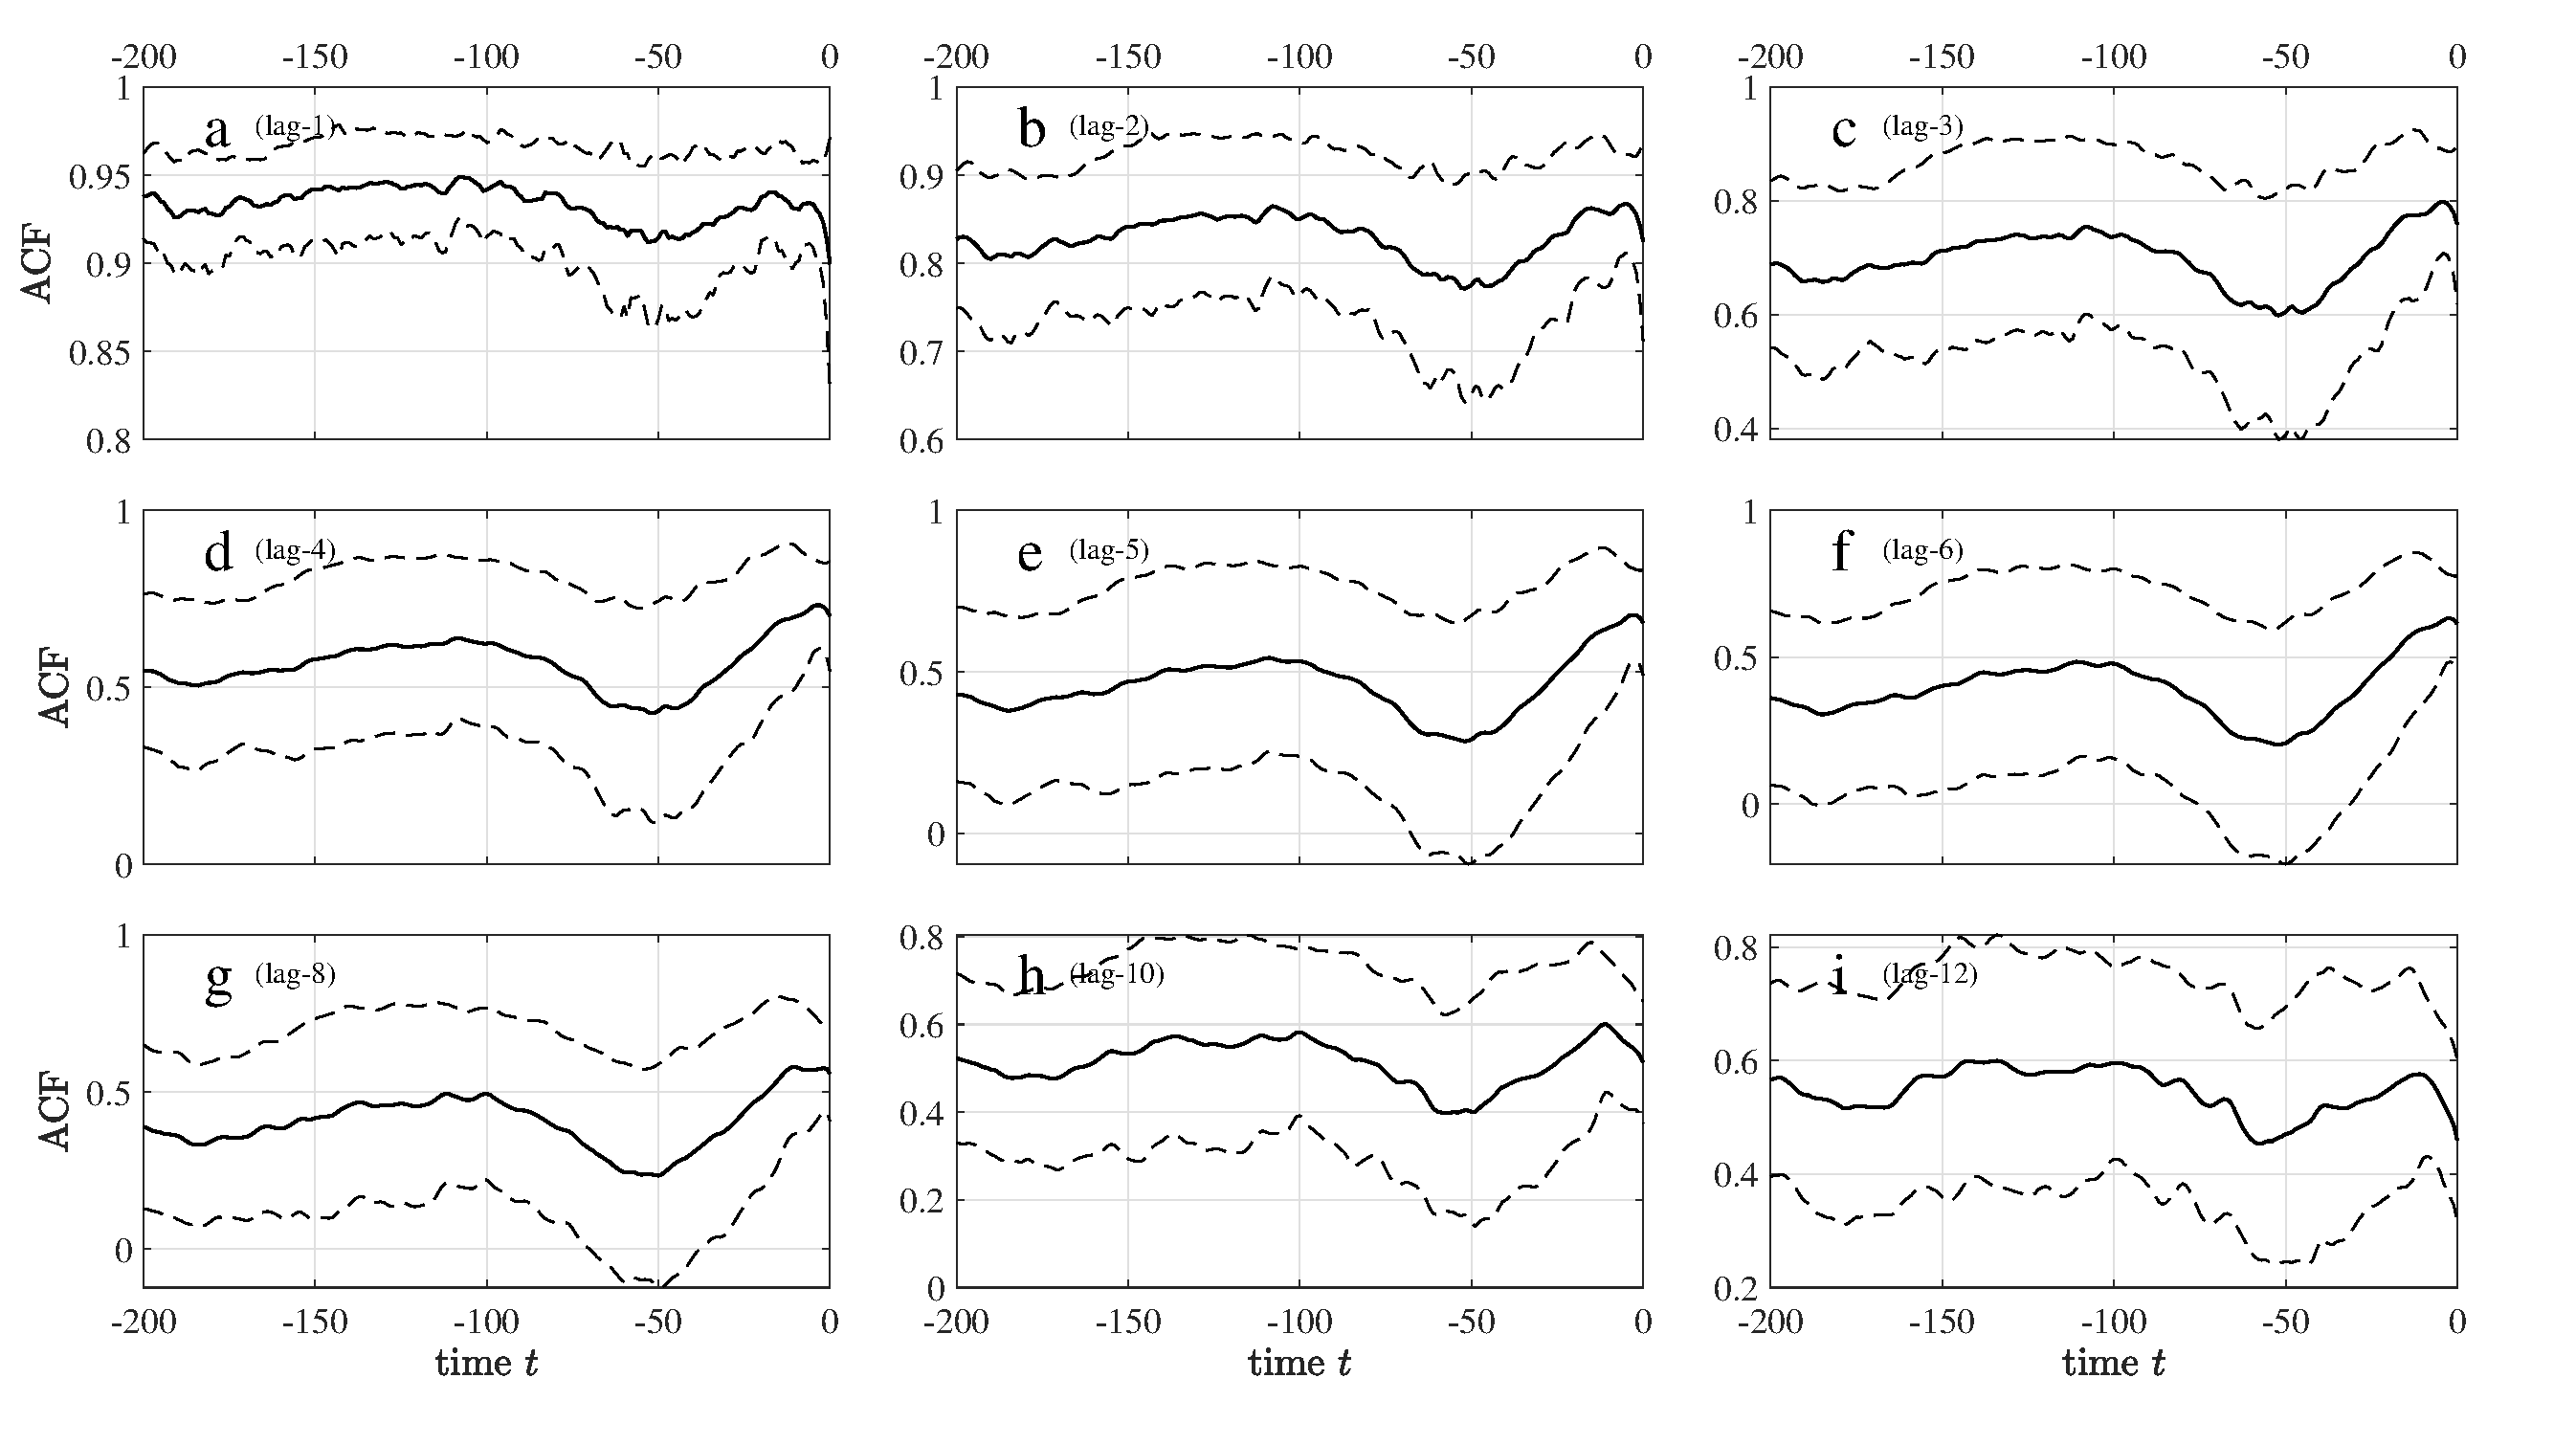
\includegraphics[width=\linewidth,keepaspectratio]{ACF_lags_comp}
		\caption{\Red{The ACF indicator is applied to the sea-level pressure time series of the fourteen tropical cyclones using an autocorrelation function with lags 1, 2, 3, 4, 5, 6, 8, 10 and 12 (in panels {\bf a}-{\bf i} respectively). The best EWS is visible when using a lag-4 ACF. }
		}
		\label{fig:TC:ACF_lags_comp}
	\end{figure}
\end{landscape}

\begin{landscape}
	\begin{figure}
		\centering
		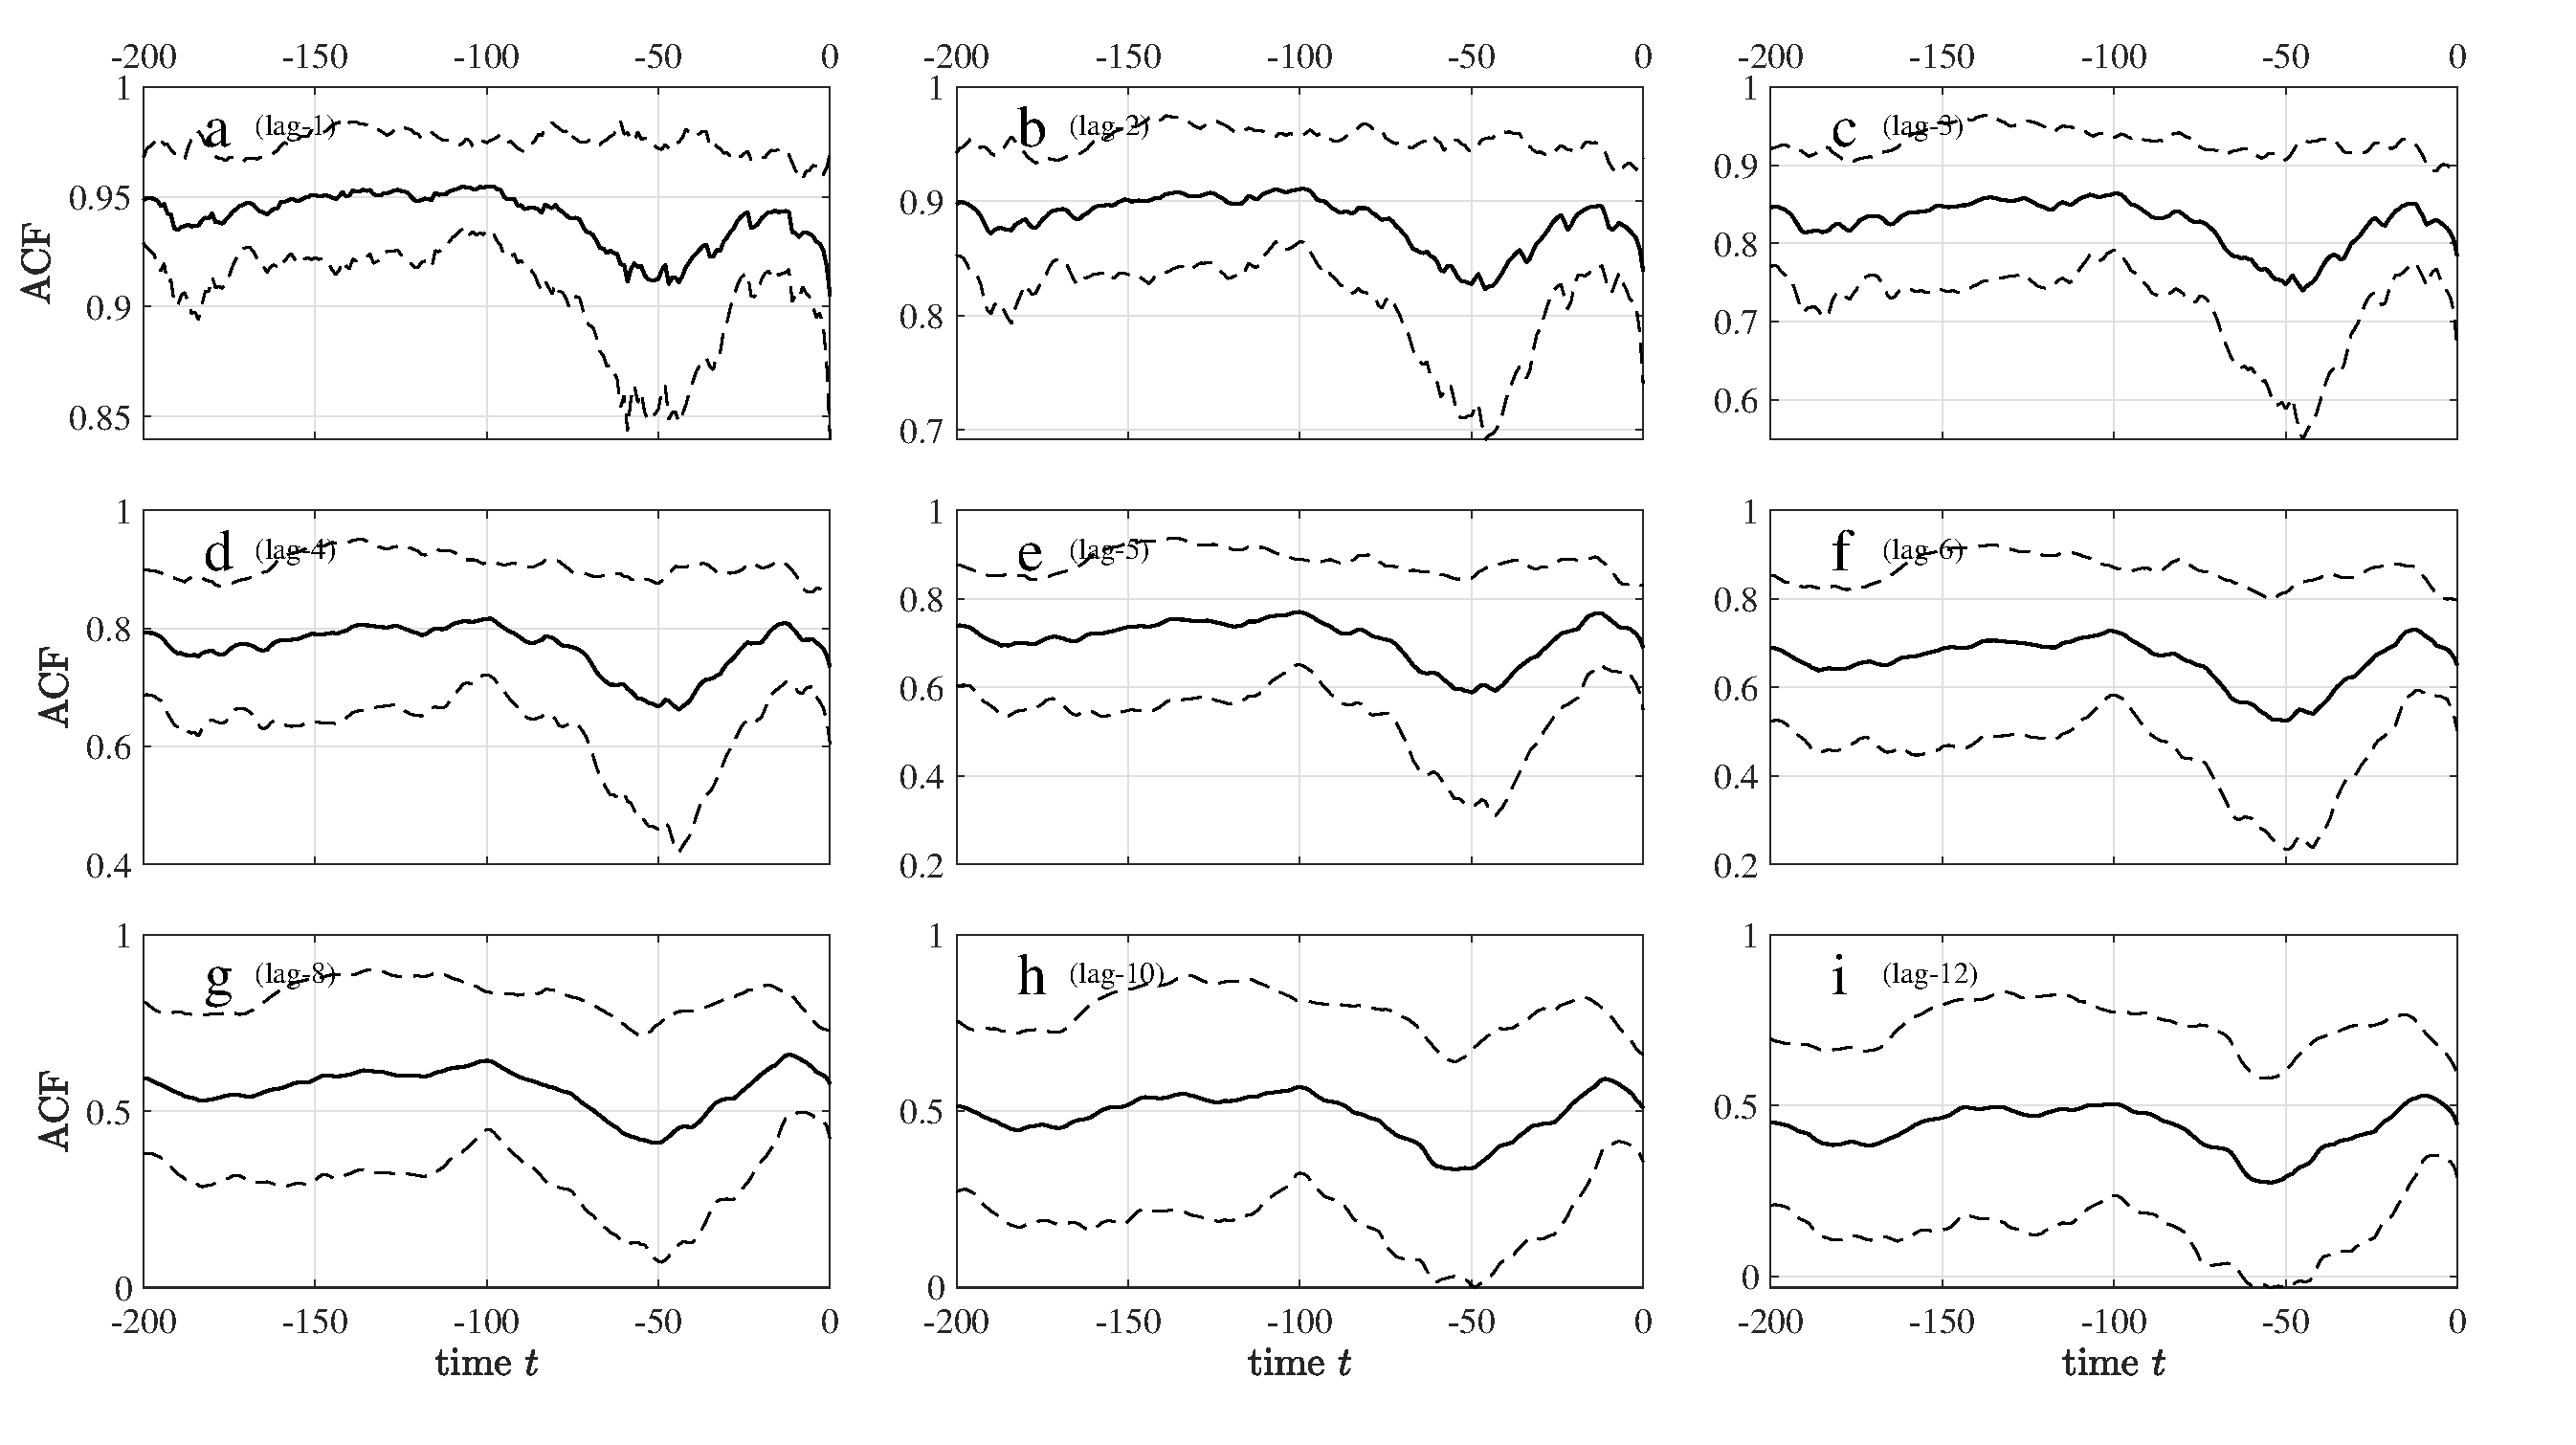
\includegraphics[width=\linewidth,keepaspectratio]{ACF_lags_comp_RO}
		\caption{\Red{A repeat of the method presented in figure~\ref{fig:TC:ACF_lags_comp}, but the oscillations have been removed from the sea-level pressure data as explained in section~\ref{subsec:TC:data:oscillations}. Again, the ACF indicator is applied to the sea-level pressure time series of the fourteen tropical cyclones using an autocorrelation function with lags 1, 2, 3, 4, 5, 6, 8, 10 and 12 (in panels {\bf a}-{\bf i} respectively). }
		}
		\label{fig:TC:ACF_lags_comp_RO}
	\end{figure}
\end{landscape}

\subsection{Sensitivity analysis}
\label{subsec:TC:1D_SA}

In order to calculate the indicator series shown in figure~\ref{fig:TC:1DindicatorsSLP}, it is necessary to select an appropriate window size. The calculation of each of the indicator series requires an appropriately large window size in order to yield an accurate calculation of the scaling exponent. The calculation of the power spectrum scaling exponent from the periodogram obtained using the fast Fourier transform is particularly inaccurate when only a small number of points are available. 

Besides the error due to the noise in the periodogram, the actual periodic spikes in the periodogram, such as the spike representing the 12-hour oscillations, have a greater influence on the calculation of the scaling exponent when fewer points are used. Furthermore, the calculation of the DFA exponent requires a minimum number of points depending on the parameters selected. The lag-1 autocorrelation could reasonably be calculated for a series of only three points, but the ACF1 indicator exhibits large variability, as with the PS and DFA indicators, for small window sizes.

It is therefore desirable to use a sufficiently large number of points to give an accurate estimate of the scaling exponent with less noisy temporal variability. However, one must attain a compromise against the competing requirement for a short time window corresponding to the time scale of the phenomenon under investigation. For example, when we consider the sea-level pressure time series in figure~\ref{fig:TC:1DindicatorsSLP} we note that the visible influence of the cyclone on the pressure begins only around 24 hours before the minimum. When attempting to detect an early warning signal, using an indicator series calculated with a window of several weeks would clearly not be useful: the large number of points relative to the actual period of interest will smooth out any significant increase or decrease. There is also a limit imposed by the length of the time series data. We require a window size such that the indicator variance is significantly small that we can see the EWS, but that the rise in the indicator value before the tipping event is large enough so that we can recognise it as an EWS.

Here we analyse the sensitivity of each indicator to the window size used, in order to ascertain the optimal window size in this particular example of a physical phenomenon, if such a universal optimum exists.

We expect that the EWS apparently becomes stronger with decreasing window size, above a certain size where the variability becomes so large that it is not possible to detect an EWS. In this way, we make a subjective choice as to the optimum window size to use in this context. The hypothesis is that all cases considered here (all fourteen cyclones and their corresponding sea-level pressure time series) are sufficiently similar in the way that the scaling exponents behave that a general optimum (or near-optimum) window size exists. In this case, it will be possible to apply these indicator methods to new data from similar sources.

It is useful to produce a contour plot of the mean value of the indicator over time, with window-size on the $y$-axis. In this way we are able to visualise hundreds of indicator series simultaneously. In figure~\ref{fig:TC:PS_sensitivity} we present the PS indicator series calculated for window sizes from 40 points to 160 points. We see that there is an increasing trend in the PS indicator towards the end of the time series with almost all window sizes. The exceptions occur periodically where the window size is a multiple of twelve: using these window sizes the indicator has a high value ($\approx1.5$) over the entire series. The most obvious early warning signals occur with window sizes which are an odd multiple of $6$, that is, 90, 102, 114, etc.. Using larger values (e.g. 174) the useful variability in the indicator is smoothed out so that the trend towards the end of the series is less obvious. We hypothesise that this 12-hour pattern is created by the 12-hour oscillations present in the sea-level pressure data, which particularly influences the power spectrum (the pattern is not observed in the ACF1 and DFA indicators, see figures~\ref{fig:TC:ACF1_sensitivity} and~\ref{fig:TC:DFA_sensitivity}). We also observe that there is a qualitative change in the nature of the pattern as the window size is increased from 99 points to 100 points, at which point, on the $y$-axis, all of the contour lines are lined up horizontally. This observation has been mentioned to the team behind the HadISD dataset, namely the authors of \cite{HadISD_dunn16}, and it has been ruled out that this is an artefact of the data collection or filtering. The investigation of the cause of this effect may be a topic for future work involving the PS indicator applied to sea-level pressure data. The 12-hour pattern serves to highlight the necessity of considering such sensitivity of the method to the window size parameter.

\begin{figure}
	\centering
	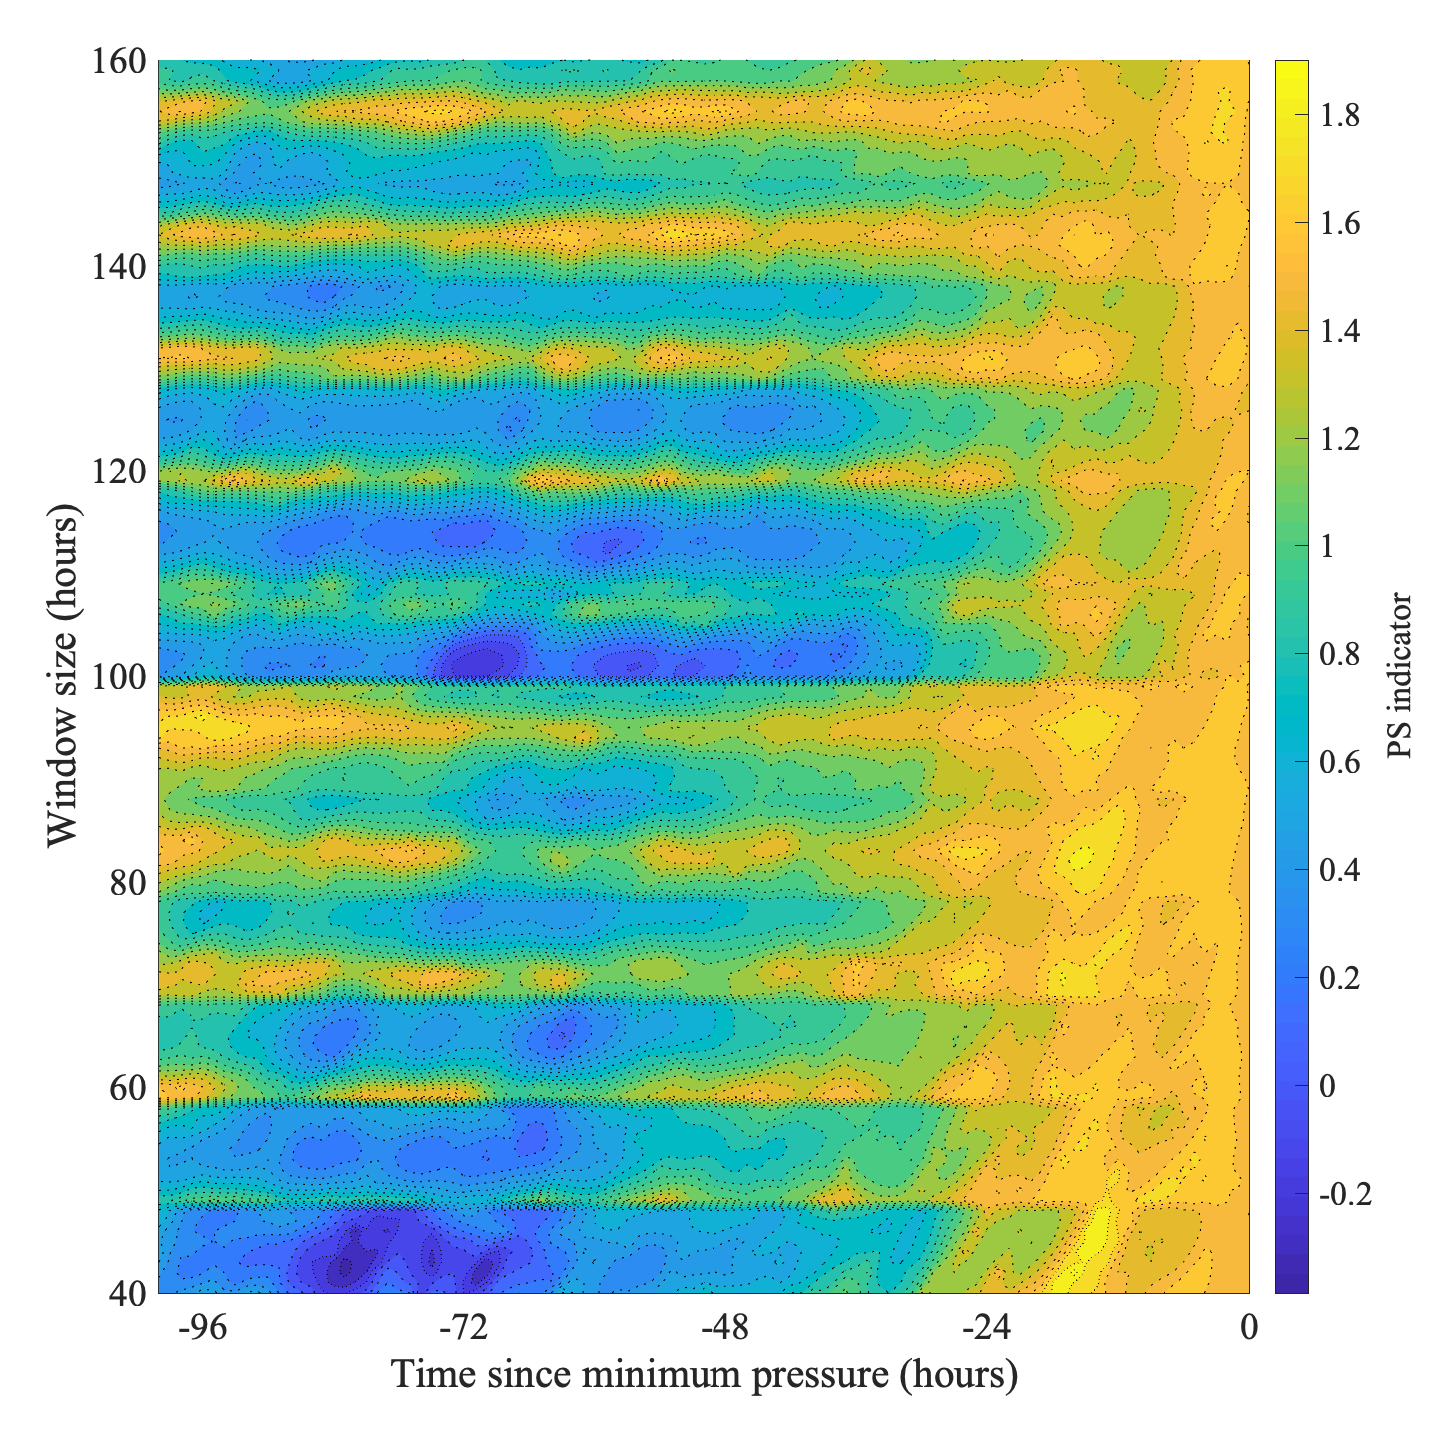
\includegraphics[width = 0.9\textwidth]{PS_sensitivity_mean}
	\caption{Mean over 14 tropical cyclones of PS indicator of the SLP data (see fig. \ref{fig:TC:1DindicatorsSLP}) calculated using window sizes from 40 to 160. The PS indicator appears to rise around 40 hours before the cyclone event in almost all cases, the exceptions occur when the window size is a multiple of 12, in these cases the indicator is high (greater than $1$) over the entire series. \label{fig:TC:PS_sensitivity}}
\end{figure}

We hypothesise that a time scale of about 100 hours, or four days, is a cut-off for the study of tropical cyclone in the context of early warning signals. A longer window encompasses too much of the time series before any forewarning signal is created, that is, before the cyclone has any influence on the autocorrelation of the sea-level pressure. Since the data available is hourly, this promotes an unfortunately short window of 100 points or fewer, which introduces a large amount of variability into the indicator series due to noise-sensitivity in the scaling exponent calculations. For this reason we proceed, in sections~\ref{sec:TC:2Dtechniques} and~\ref{sec:TC:field_data}, to incorporate more data into the calculation of a tipping point indicator series.

In keeping with the decision to select a window size of about 100 points, we selected a window size of 102 points when calculating the PS indicator in figure~\ref{fig:TC:1DindicatorsSLP}. At 90 points, the indication does not provide such an obvious early warning signal. In figure~\ref{fig:TC:PS_windows_indicators} we present the PS indicator, as in figure~\ref{fig:TC:1DindicatorsSLP}d, but using window sizes of 54, 90, 102 and 150 points (in panels \textbf{a}, \textbf{b}, \textbf{c} and \textbf{d} respectively). Since the fast Fourier transform periodogram is a less accurate approximation of the power spectrum when using fewer points, we might expect there to be greater variability when using a short window: both less agreement between the fourteen time series, and more variability within each individual time series along the time scale. We observe, in figure~\ref{fig:TC:PS_windows_indicators}, that the former is not apparently the case: the size of the error bars, which is one standard deviation over the fourteen sea-level pressure series, is largest when using a window size of 102 points, which is our chosen value based on the more obvious early warning signal in the mean. 

In figure~\ref{fig:TC:stdSensitivity} we investigate in what way the variance in the indicator series is effected by the window size. We expect, since the estimation of the DFA and PS scaling exponents is less accurate for shorter time series, that using a shorter window would result in a noisier indicator series, regardless of the nature of the input data. For each window size we calculate the standard deviation in the indicator series for each of the fourteen tropical cyclones, then take the mean of the fourteen values of standard deviations. The indicator series is calculated between 300 hours and 48 hours before the event, so that any anticipated increase prior to the event (in the 48 to 0 hours range) is not confused with noise. The hypothesis proves correct for the DFA indicator, shown in red, until the window size reaches around 100 points, after which the standard deviation remains constant. For the PS indicator, the standard deviation also decreases with increasing window size, as expected, but jumps up again for window size 100 points, after which it continues to decrease steadily. This jump is presumably related to the qualitative change in the mean which also occurs at window size 100 points (see figure~\ref{fig:TC:PS_sensitivity}). As we have remarked above, it is not know why this occurs but the investigation of the effect is an interesting topic of future work. 

The PS indicator series is less noisy for window size 90 points, and also has less variability across the fourteen cyclones, than for 102 points. However, this must be balanced by the consideration that the early warning signal, if present at all, is more obvious in the 102 point window series. 

\begin{figure}
	\centering
	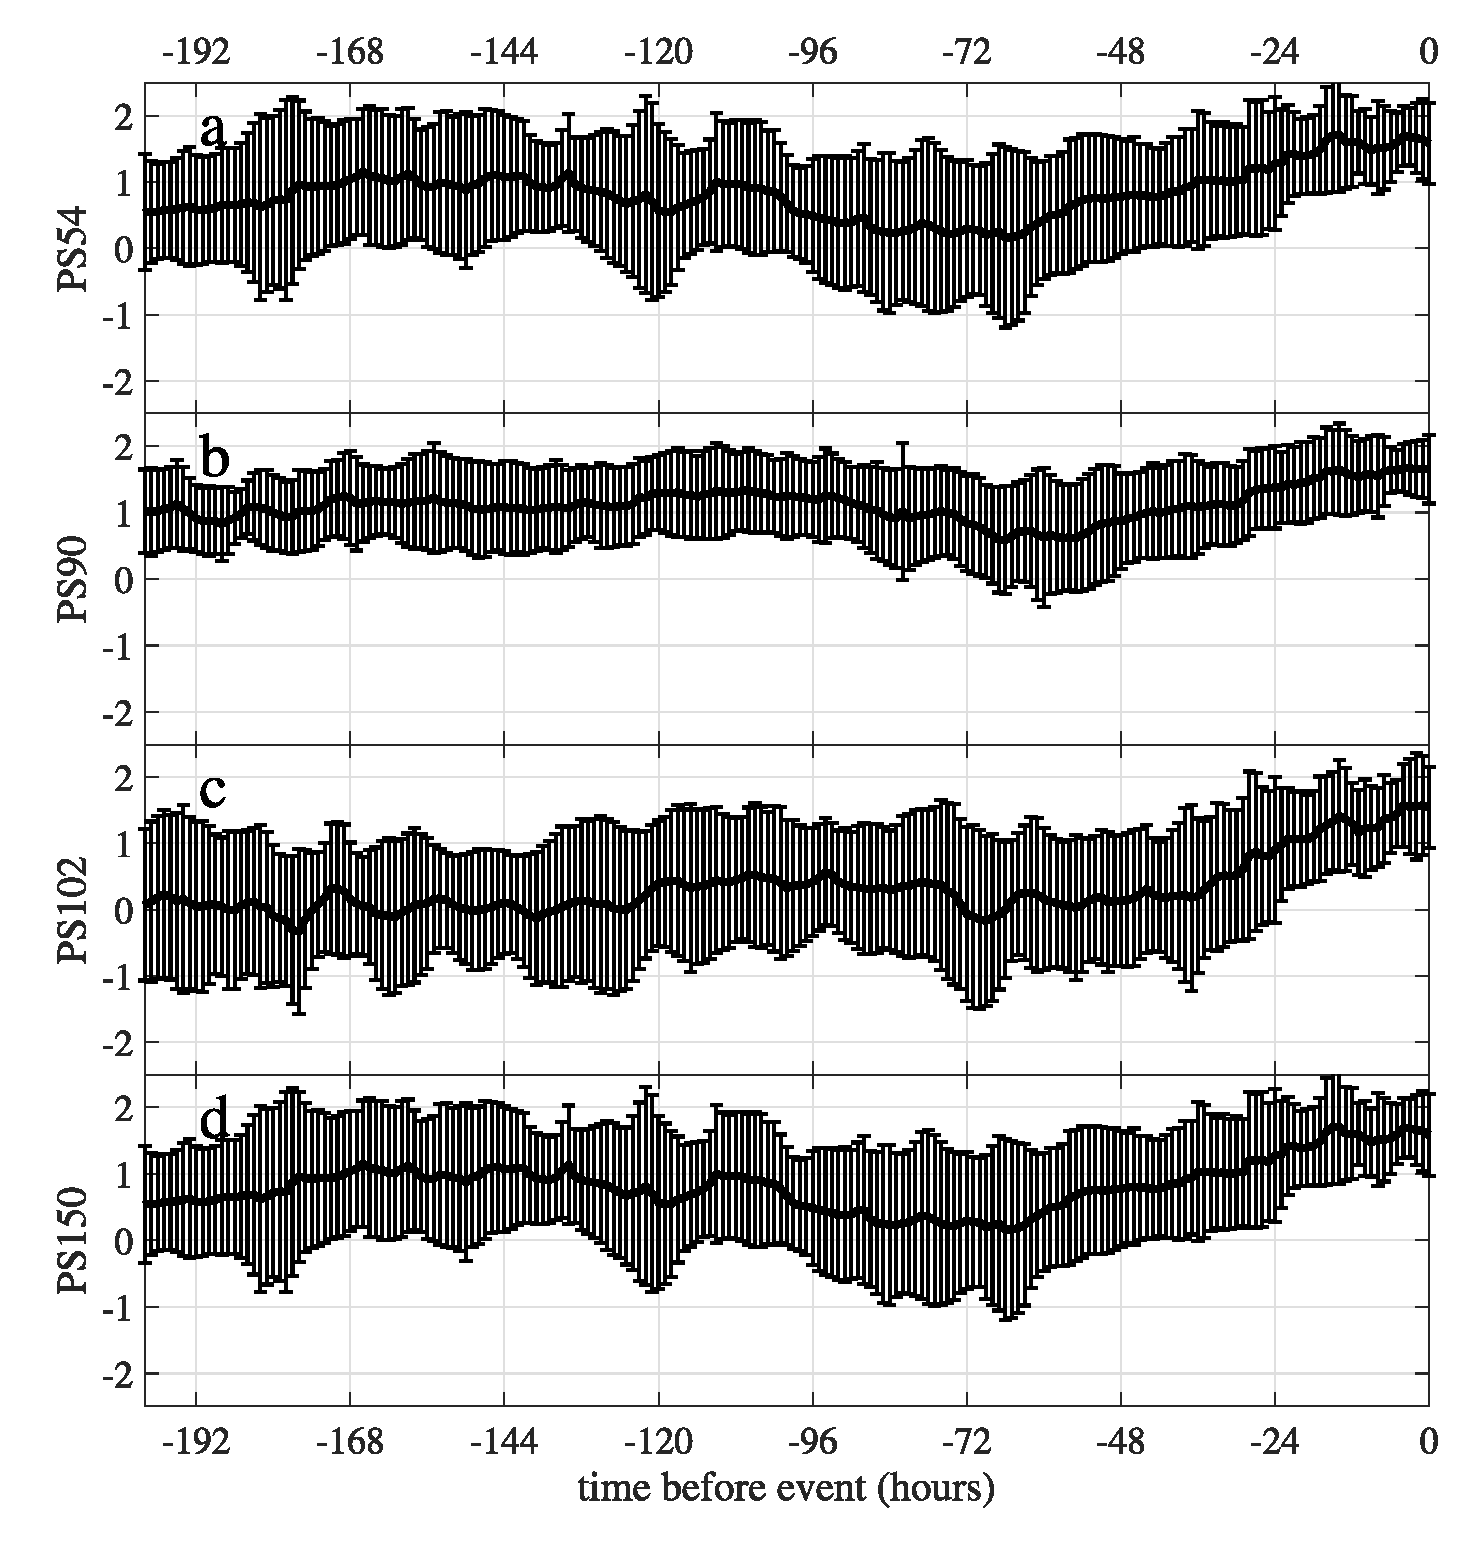
\includegraphics[width = 0.9\textwidth]{PS_windows_indicators}
	\caption{The PS indicator is calculated for the fourteen tropical cyclone sea-level pressure series and the mean, with error bars of one standard deviation, is shown. The method is the same as in figure~\ref{fig:TC:1DindicatorsSLP}d, but using window sizes 54, 90, 102 and 150 points (in panels \textbf{a}, \textbf{b}, \textbf{c} and \textbf{d} respectively). \label{fig:TC:PS_windows_indicators} }
\end{figure}

\begin{figure}
	\centering
	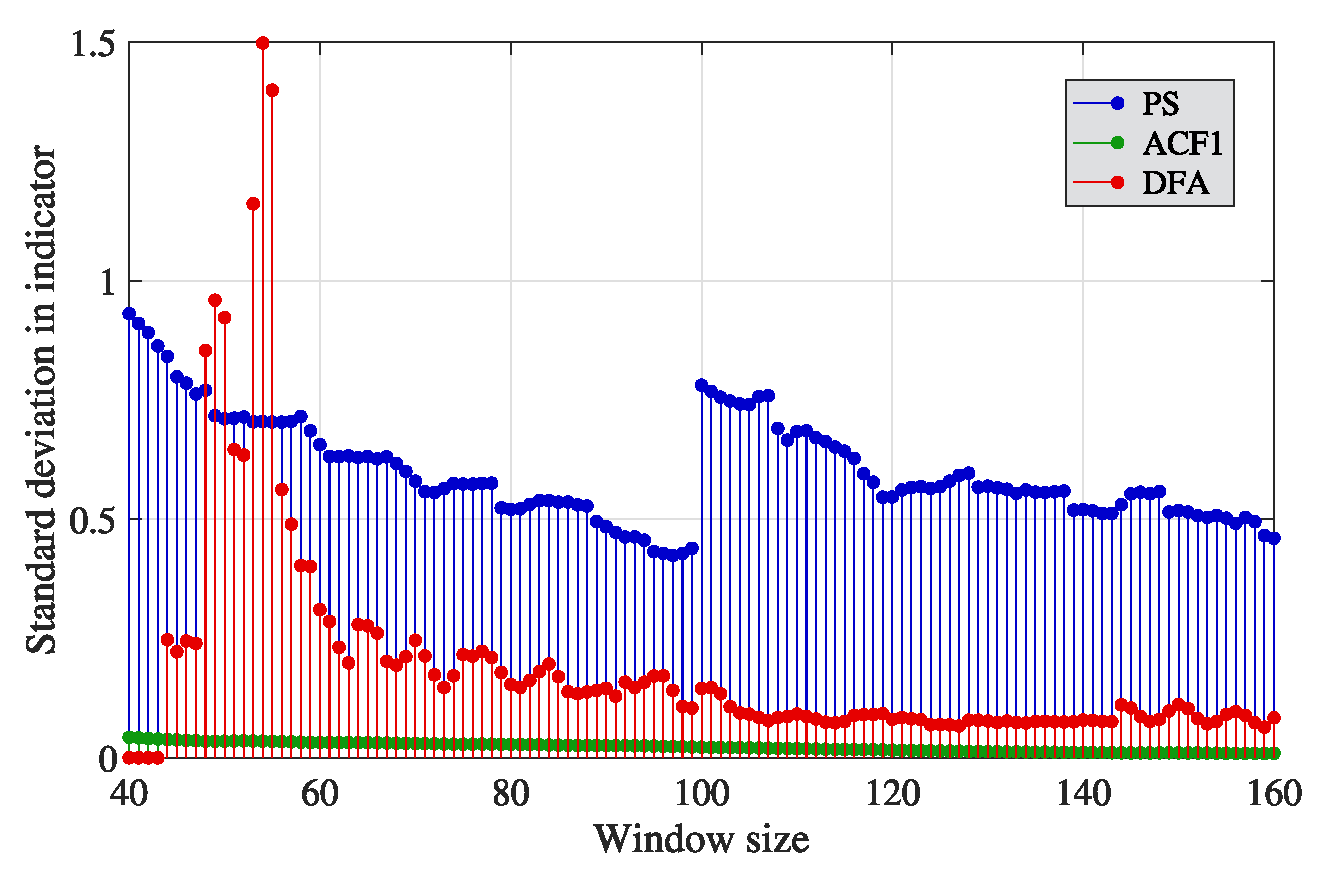
\includegraphics[width = 0.9\textwidth]{stdSensitivity}
	\caption{Sensitivity of the variance in the tipping point indicators to window size. For each window size the standard deviation in the indicator series is calculated for each of the fourteen tropical cyclones and the mean over the fourteen values is plotted.
		\label{fig:TC:stdSensitivity} }
\end{figure}

Figure~\ref{fig:TC:ACF1_sensitivity} is produced by the same method as figure~\ref{fig:TC:PS_sensitivity} but uses the ACF1 indicator. The range of window sizes is also smaller: from 40 to 120, because for sizes over 120 the indicator was consistently above 0.95 and showed no change over the time period. In this case, we notice that the indicator rises, for all window sizes, to a maximum value at around 16 hours before the event, before decreasing sharply. Unfortunately there is something just before -100 hours which causes the ACF1 indicator, particularly with a window size above 60, to be very high –higher than the highest value immediately preceding the cyclone event– which is not visible in the PS and DFA indicators (figures~\ref{fig:TC:PS_sensitivity} and~\ref{fig:TC:DFA_sensitivity}). {\Red{The same pattern is evident in figure~\ref{fig:TC:ACF4_sensitivity} where the ACF4 indicator has been used rather than the ACF1 indicator (that is, the lag-4 autocorrelation function is used in the calculation) since the results presented in figure~\ref{fig:TC:ACF_lags_comp} (see page~\pageref{fig:TC:ACF_lags_comp}) show that a better EWS is visible when lag-4 ACF is used. We note that in this case the value of the indicator is lower (<0.9) over most of the time series and so the increase just before the tipping event is more visible. Additionally, the sharp decrease at the end of the ACF1 indicator signals is not present in the ACF4 indicator signals. }}

\begin{figure}
	\centering
	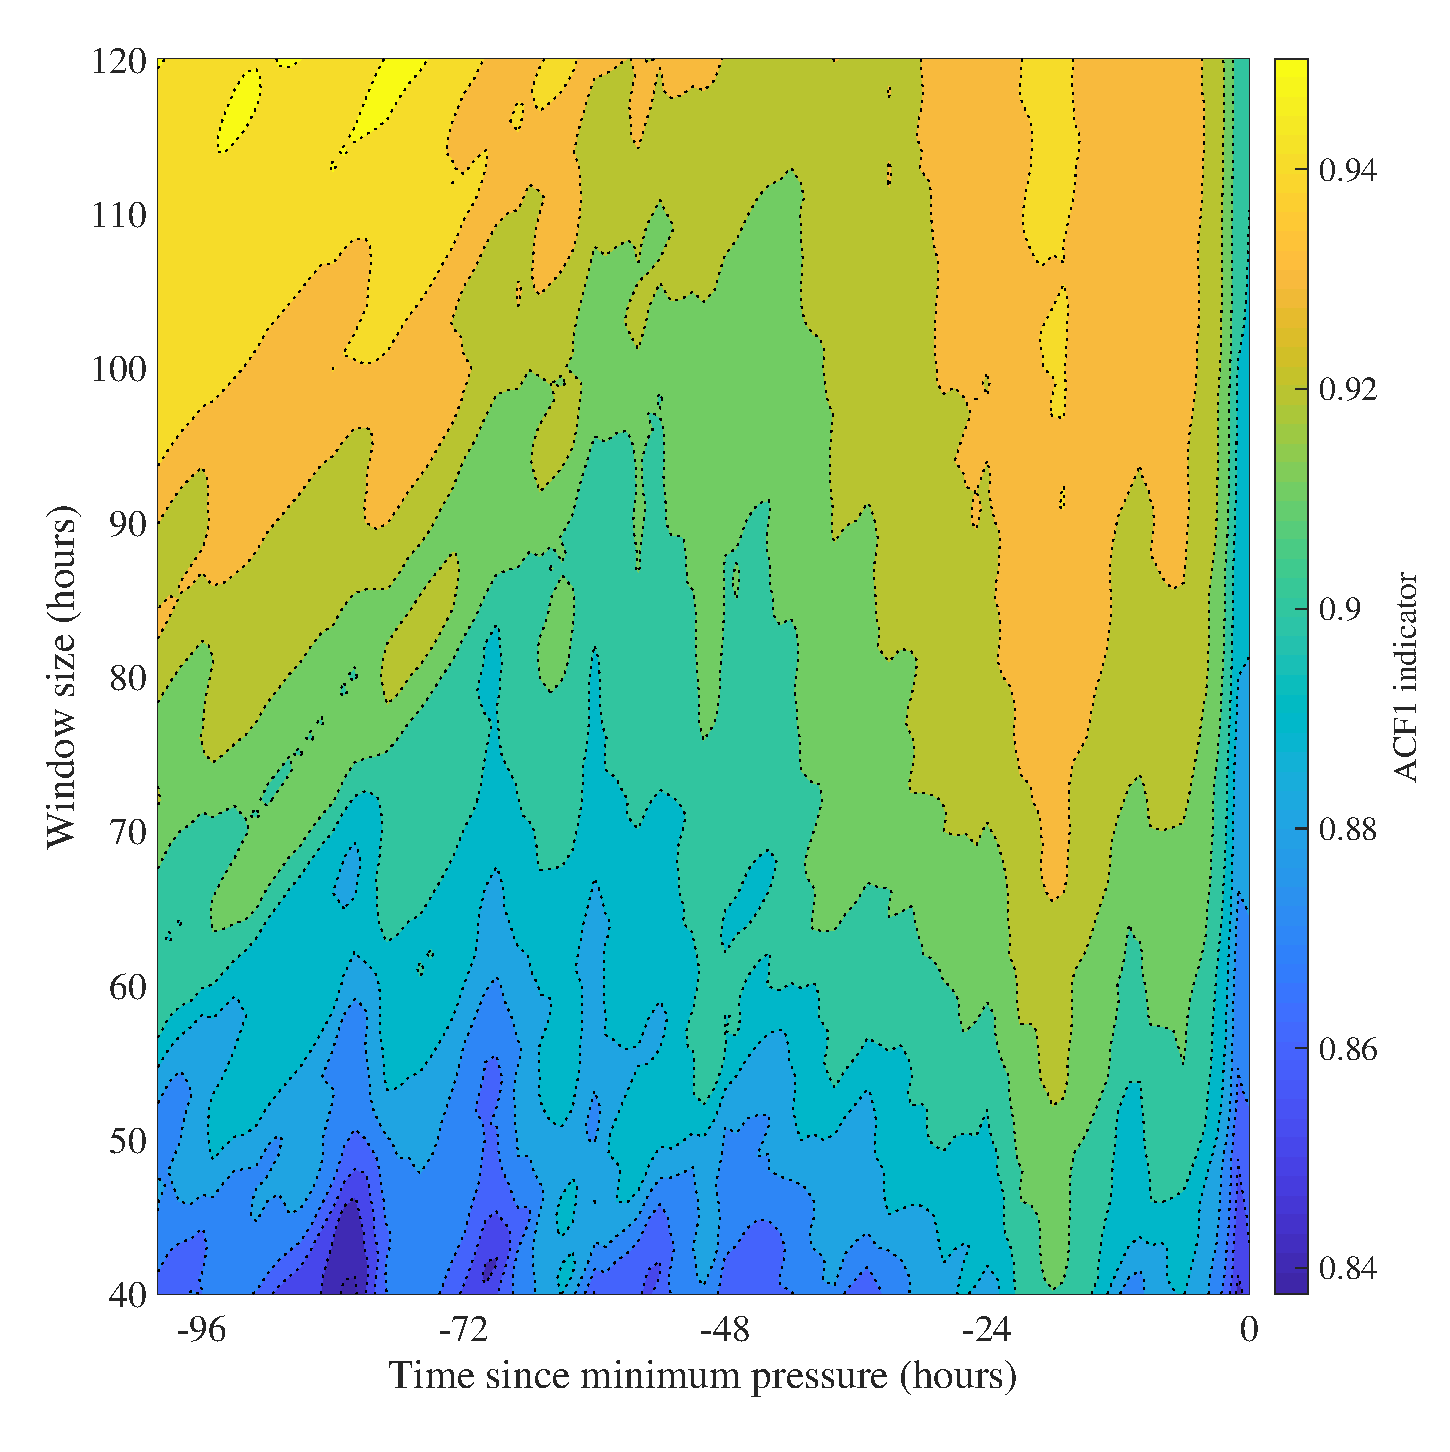
\includegraphics[width = 0.9\textwidth]{ACF1_sensitivity_mean}
	\caption{Mean over 14 tropical cyclones of the ACF1 indicator of the SLP data (see fig. \ref{fig:TC:1DindicatorsSLP}) calculated using window sizes from 40 to 120. The ACF1 indicator appears to rise around 30 hours before the cyclone event in almost all cases. The increase is more pronounced when using a larger window size. \label{fig:TC:ACF1_sensitivity}}
\end{figure}

\begin{figure}
	\centering
	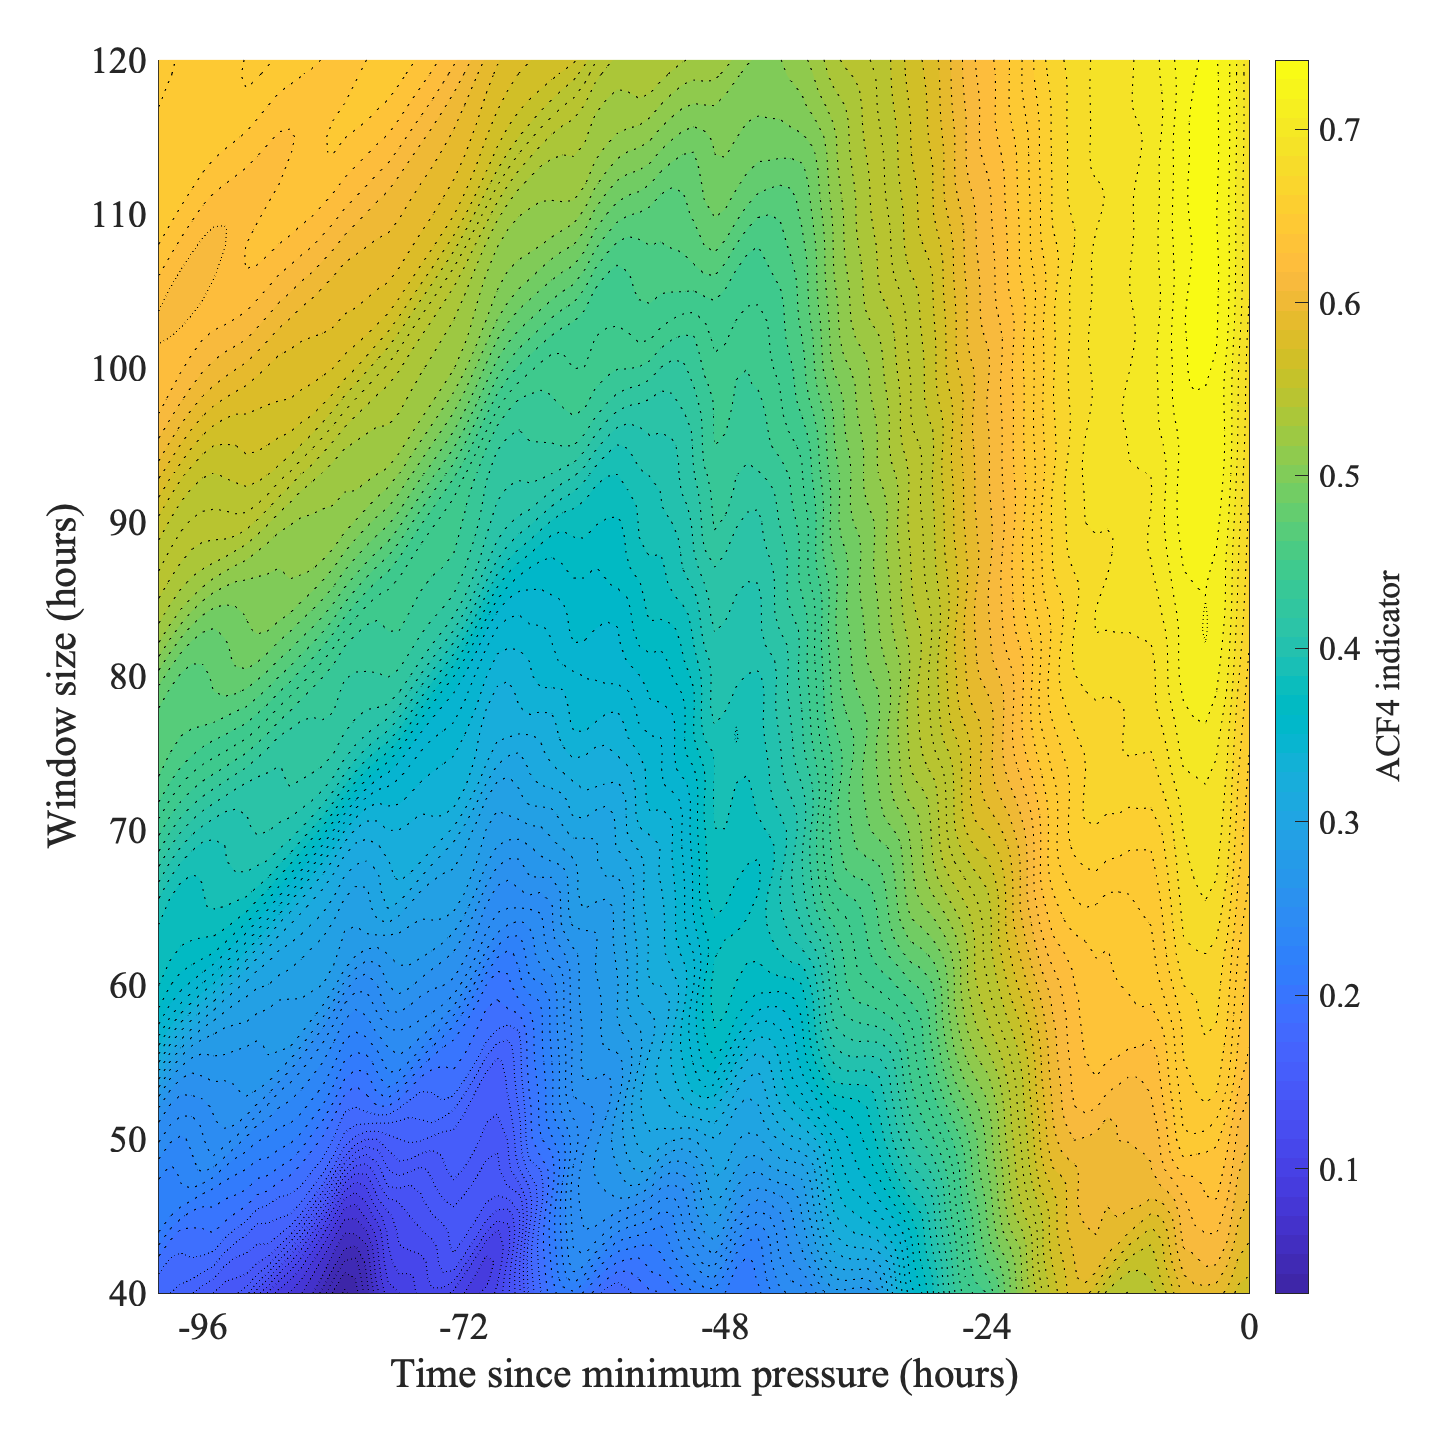
\includegraphics[width = 0.9\textwidth]{ACF4_sensitivity_mean}
	\caption{\Red{Mean over 14 tropical cyclones of the ACF4 indicator (using lag-4 autocorrelation) of the SLP data (see fig. \ref{fig:TC:1DindicatorsSLP}) calculated using window sizes from 40 to 120. The ACF1 indicator appears to rise around 30 hours before the cyclone event in almost all cases. The increase is more pronounced when using a larger window size. We note a similar pattern to the ACF1 indicator in figure~\ref{fig:TC:ACF1_sensitivity}, but the picture is clearer and a clear increase in the indicator can be observed before the tipping event even using very short window sizes.  }}
	\label{fig:TC:ACF4_sensitivity}
\end{figure}

Figure~\ref{fig:TC:DFA_sensitivity} is produced using the DFA indicator, again with a range of window sizes from 40 to 120. The calculation of the DFA scaling exponent is not possible for very short series, depending on how the series is segmented before each segment is detrended by subtracting a polynomial\footnote{In this study we consistently use quadratic detrending to address non-linear effects.}. So as to be able to estimate the scaling exponent, we use eight different segment sizes increasing logarithmically from the smallest to the largest, the smallest being ten points and the largest being $\lfloor N/4\rfloor$ where $N$ is the length of the series. In this way it is always possible to get at least four segments from the series. Using this method it does not make sense to calculate the DFA exponent with a series shorter than 44 points because only one distinct segment size is used, 10, and therefore the relationship between the segment size and the fluctuations coefficient is estimated from a single point.

Table~\ref{tab:TC:DFAsegmentSizes} shows the eight segment sizes used for series lengths 40, 54, 100 and 400. A series length of at least 400 would be ideal, giving a range of segment sizes between 10 and 100 with which to be able to calculate the correlation between the segment size and fluctuations coefficient (see section~\ref{subsec:1D:scaling_exponents:DFA}). With the available data for the sea-level pressure, a window size of 400 points cannot be used. We use a window size of 90 points because there appears to be a slightly stronger early warning signal (an increase in the indicator prior to the event) than with other window sizes. However, the DFA indicator is practically useless when applied to this data.

A series length of 54 is considered in table~\ref{tab:TC:DFAsegmentSizes} because there appears to be interesting oscillating behaviour in figure~\ref{fig:TC:DFA_sensitivity} with a window size of 54. The oscillation has a period of six hours, which suggests a connection with the 12-hour oscillations present in the sea-level pressure data. We also note that there is a qualitative change in the behaviour of the DFA indicator as the window size reaches 80, 91 and (more weakly) 100 points, similar to the change observed in the PS indicator at 100 points (see figure~\ref{fig:TC:PS_sensitivity}). Again, it is not known why this occurs and should be the subject of further investigation. 


\begin{figure}
	\centering
	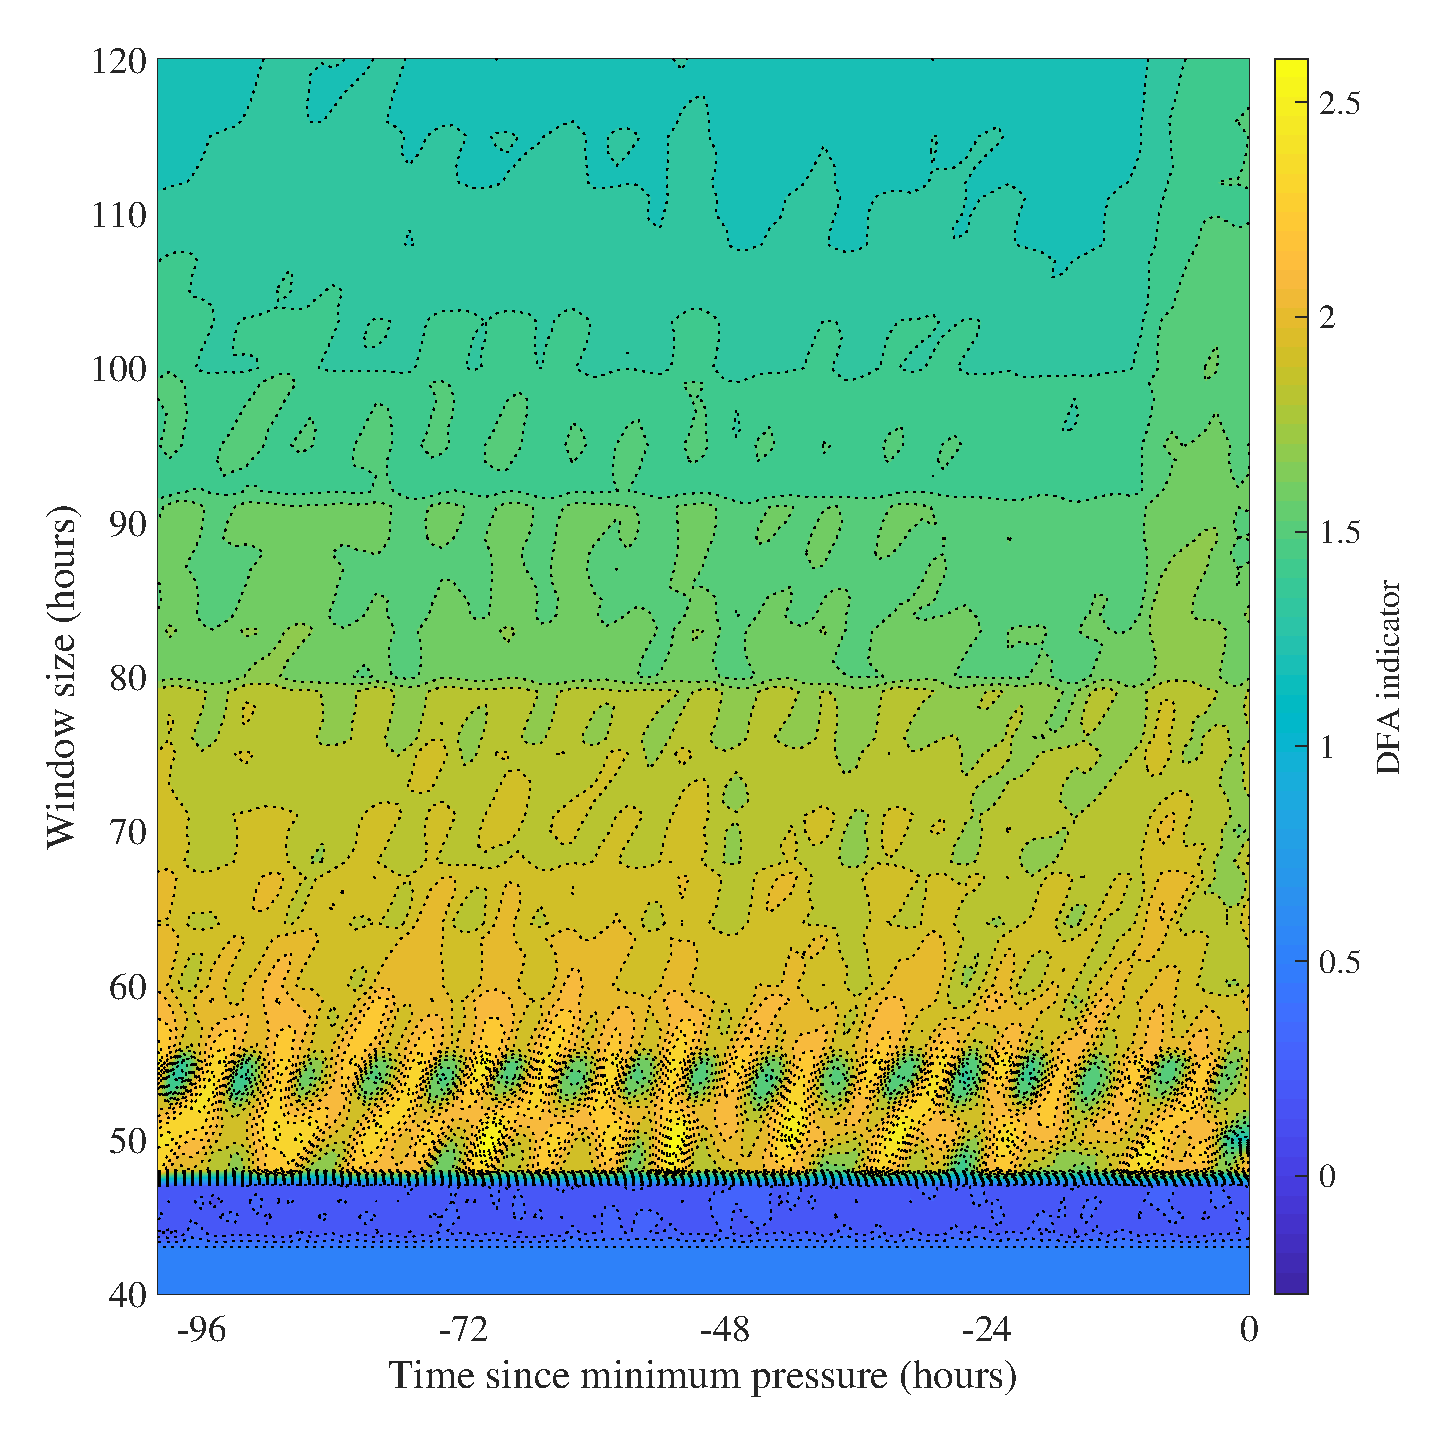
\includegraphics[width = 0.9\textwidth]{DFA_sensitivity_mean}
	\caption{Mean over 14 tropical cyclones of DFA indicator of the SLP data (see fig. \ref{fig:TC:1DindicatorsSLP}) calculated using window sizes from 40 to 120. There is a very small apparent rise in the DFA indicator at -12 hours for window sizes greater than 80 hours. \label{fig:TC:DFA_sensitivity}}
\end{figure}


\begin{table}
	\centering
	\begin{tabular}{c l}
		\hline
		Series length & Segment sizes\\
		\hline
		40  & 10\\
		54  & 10, 11, 12\\
		100 & 10, 11, 12, 14, 16, 19, 21, 25\\
		400 & 10, 13, 19, 26, 37, 51, 71, 100\\
		\hline
	\end{tabular}
	
	\caption{During the calculation of the DFA scaling exponent, a series of length $N$ is segmented eight times, the sizes of the non-overlapping segments increase logarithmically from 10 to $\lfloor N/4\rfloor$. The segment sizes used for four example series lengths are shown. For very short series, fewer than eight different segment sizes may be used.}\label{tab:TC:DFAsegmentSizes}
\end{table}

%\subsection{Investigating autocorrelation with different lags}
%\label{subsec:TC:1D_Lags}
%{\noteRed Maybe? not much to see.}


\section{Application of multi-variable tipping point techniques}
\label{sec:TC:2Dtechniques}

In this section we consider the same fourteen tropical cyclones detailed in table~\ref{tab:TC:14cyclones}. In section~\ref{sec:TC:1Dtechniques}, tipping point indicators were applied to the one-dimensional time series of the sea-level pressure variable at each station. Here, both the wind speed and sea-level pressure are considered together. We first calculate the ACF1, DFA and PS indicator series for the wind speed variable. Using the exact same process by which figure~\ref{fig:TC:1DindicatorsSLP} was produced, showing the indicator series for the sea-level pressure variable, we produce figure~\ref{fig:TC:1DindicatorsWS}, showing the indicator series for the wind speed variable. The same window sizes were used for the ACF1, DFA and PS indicators (90, 90, 102 respectively) as for the sea-level pressure. We note that the mean ACF1 and PS indicators rise with the rising wind speed, and that the DFA indicator performs similarly as in the sea-level pressure case. None of the indicators appear to provide an early warning signal, so we do not expect that combining the wind speed and sea-level pressure variables will yield a signal stronger than already present in the sea-level pressure. However, we proceed to investigate the results of the multi-variable tipping point analysis in comparison to the analysis of the individual variables. 

Throughout this section, including in figure~\ref{fig:TC:1DindicatorsWS}, the time series are aligned so that $t=0$ occurs at the point where the sea-level pressure is minimum, for consistency when comparing to the results in the previous section. This may not be the same point at which wind speed is maximum. {\Red{The results presented in this section have previously been published in \cite{prettyman2019}.}}

\begin{figure}
	\centering
	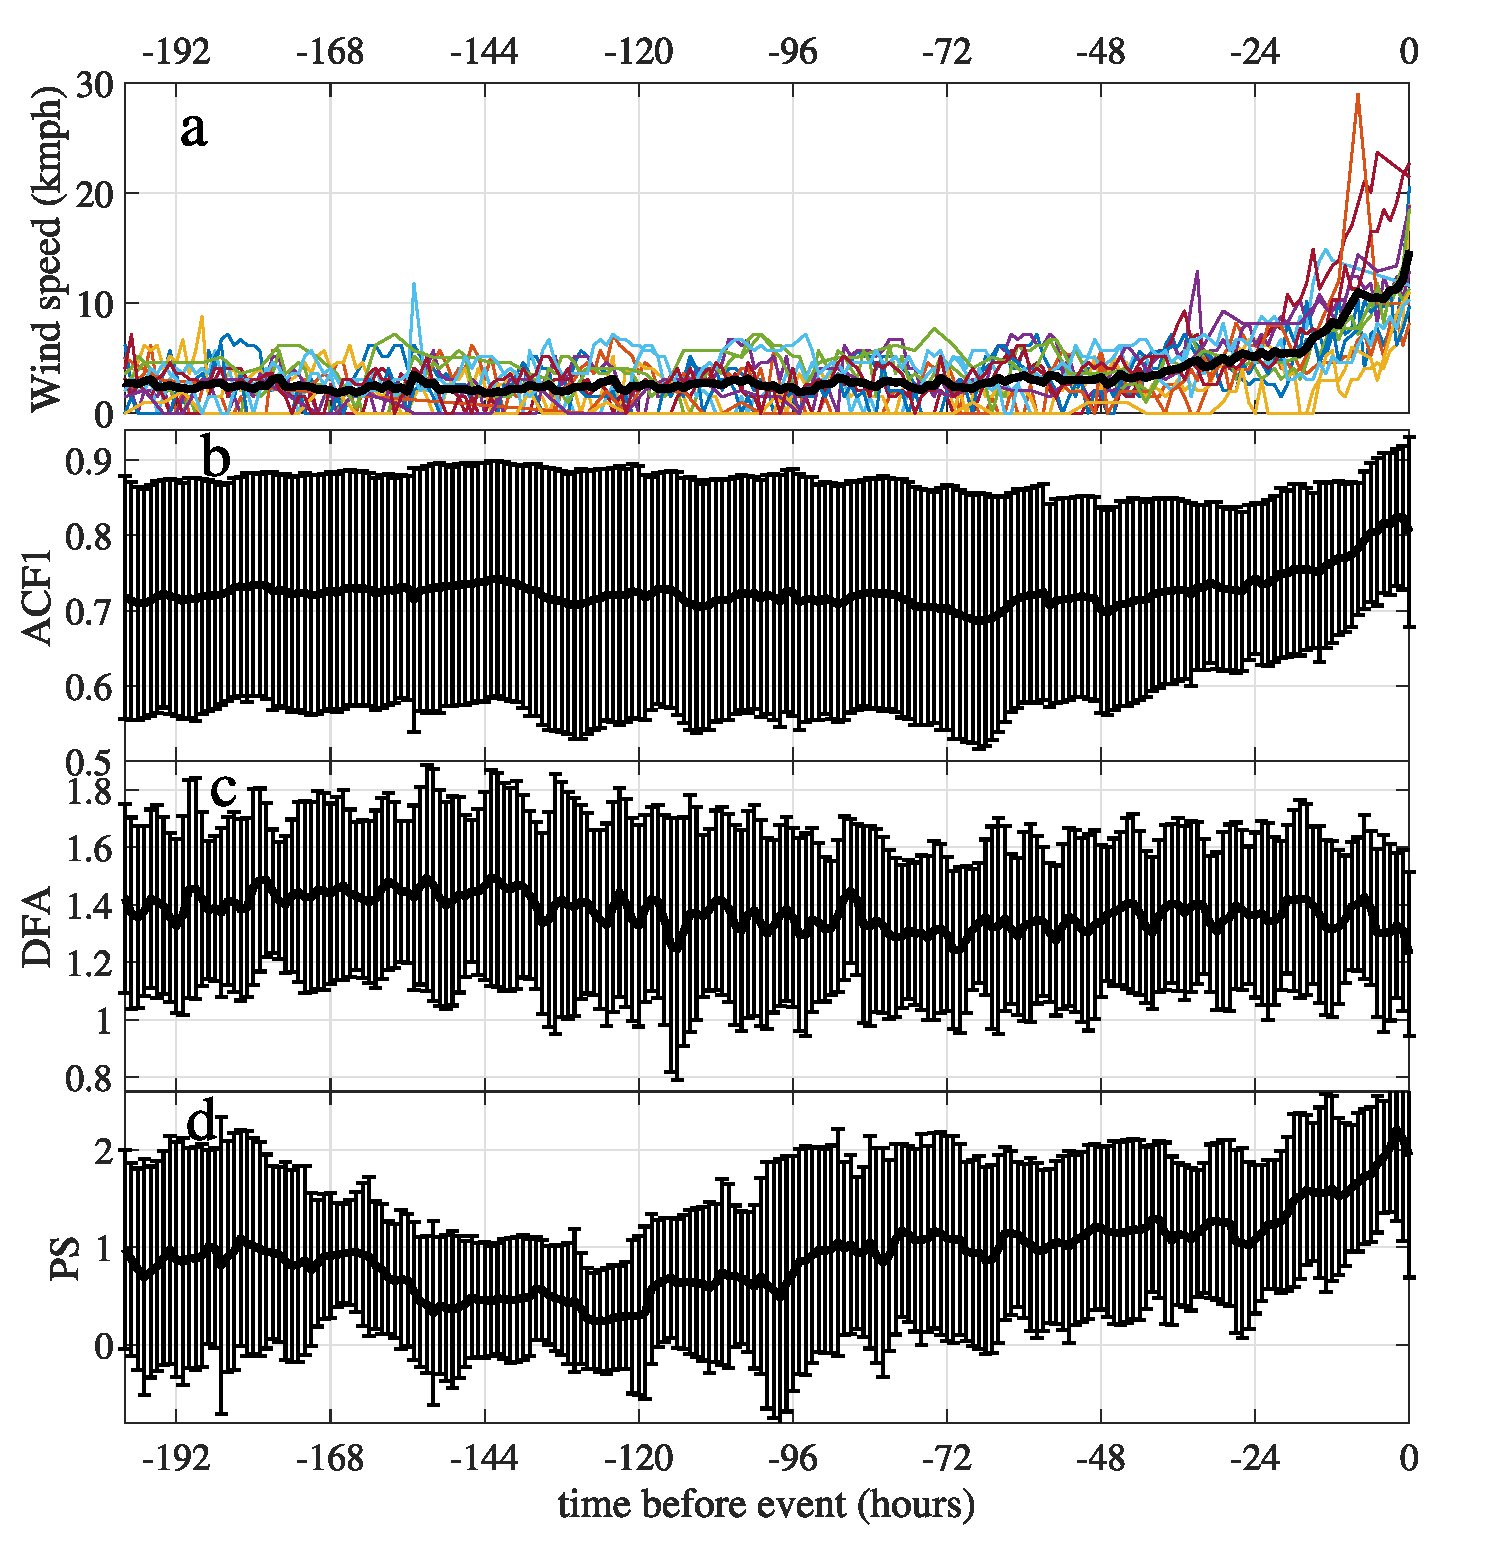
\includegraphics[width = 0.9\textwidth]{indicators14_windspeed}
	\caption{Wind speed data from fourteen tropical cyclones and the mean ACF1, DFA and PS indicators. (a) Wind speed data from the 14 tropical cyclones, mean shown in black. (b,c,d) The mean ACF1, DFA and PS indicators, with error bars of 1 standard deviation. \label{fig:TC:1DindicatorsWS}}
\end{figure}

\subsection{Method}
\label{subsec:TC:2Dmethod}

Having considered the sea-level pressure and wind speed variables separately (figures~\ref{fig:TC:1DindicatorsSLP} and~\ref{fig:TC:1DindicatorsWS}) we now combine the two variables so that more data is available from which to produce a single tipping point indicator series. We use the the methods introduced in sections~\ref{sec:2D:Williamson} and~\ref{sec:2D:EOF}, that is, the analysis of the eigenvalues of the Jacobian matrix of a linearised system, and the use of EOFs to reduce the dimension before applying the one-dimensional indicator techniques.  

\subsubsection{Jacobian eigenvalues analysis}
For the Jacobian eigenvalues analysis we repeat the method described in section~\ref{sec:2D:Williamson} using a window size of 102 points in order to provide a comparison with the PS indicator applied to the one-dimensional sea-level pressure time series, for which this window size is used. In section~\ref{subsec:TC:2D_SA} we will perform a sensitivity analysis to determine whether a different window size is preferable. Besides the window size, it is necessary to choose whether to study the real part, the imaginary part, or the complete complex eigenvalue. Since we do not know in advance the nature of the tipping, we record both the real and imaginary parts. Thus, in a sliding window of 102 points, the Jacobian matrix of the linearised system is estimated from the two system variables (sea-level pressure and wind speed) and the principal eigenvalue is recorded. The method of approximating Jacobian eigenvalues has previously been applied to dynamical systems where the governing equations and the type of bifurcation are known \citep{williamson2015}, and so we know in advance what type of signal we should expect, such as with the example of the Van der Pol oscillator in the previous chapter (figure~\ref{fig:2D:vdpIndicators}). However, we have noted that the method was intentioned as a two-dimensional analogue to the lag-1 autocorrelation, so it is reasonable to apply it to systems in which the one-dimensional ACF1 indicator, and the related PS and DFA indicators, increase prior to a tipping point. We are particularly interested to note the extent to which this indicator is an improvement, if at all, over simply considering the one-dimensional indicators individually, and whether any additional artefacts arise as a consequence of considering the two variables together.

\subsubsection{Dimension reduction using EOFs}
The other technique we use here is to first obtain the the leading EOF score of the two time series (sea-level pressure and wind speed) in order to reduce the dimension to one. The time series in both variables are first mean-centred, as per the EOF method, and also normalised in order to non-dimensionalise. We are then able to apply the one-dimensional EWS techniques, the ACF1 and PS indicators, and take the mean over all cyclones. We use a window size of 102 for the PS indicator and 90 for the ACF1 indicator, since these were found to be useful when considering the sea-level pressure alone in the previous section.

As noted in section~\ref{subsec:2D:EOF:movingEOF}, there are three available approaches to obtaining the principal EOF score, that is, there are three approaches to obtaining the vector onto which we project the two-variable series. The vector is the principal eigenvector of the covariance matrix of two time series, we may use either
\begin{enumerate}
	\item the entire available time series (global projection), or
	\item only the segment of the time series in each window (windowed projection), or
	\item the entire available time series \emph{up to} the end of the current window (moving projection).
\end{enumerate}
The first option in this case implies using the part of the time series which lies in the "future" of the current window. This is not comparable to practical prediction problems and so we avoid it here. It is also not sensible to obtain the projection vector using the part of the time series which includes the tipping point when considering the rest of the series, because the dynamics are not representative. 

The second and third options are distinguished in section~\ref{subsec:2D:MethodsApplied:Hopf_movingEOF}. The windowed projection most accurately captures the maximum variance in each window, but may be unsuitable if the principal EOF eigenvector is highly variable due to noise. In this system we want to avoid considering signals from meteorological events prior to the tropical cyclone being studied and want to, as much as possible, consider a relatively stationary system prior to the tipping event. To this end, we generally truncate the time series at around 300 hours before the tipping point and so the total length of the series is not much longer than the window size used in the indicator calculation (approximately 100 hours). Therefore, the difference between using the windowed or moving projection will be negligible. Throughout this section, we use the windowed projection.

Since the two variables have different units, it is not meaningful to consider them together without first non-dimensionalising. To satisfy this requirement, as part of the EOF technique, each time series is mean-centred and normalised by its own standard deviation. In section~\ref{subsec:TC:2D_SA} we explain the investigation into the effect of weighting the two variables differently, as a result of which we choose to weight the sea-level pressure and wind speed variables in the ration $40:60$ when using the ACF1 indicator, and to weight the variables equally when using the PS indicator.

\subsection{Results}
\label{subsec:TC:2Dresults}

The Jacobian eigenvalue analysis is performed separately for each cyclone and both the real and imaginary parts of the principal eigenvalue are recorded. The mean of the fourteen resulting indicator series is shown in figure~\ref{fig:TC:indicators_WLandEOF}a,b, with error bars of one standard deviation over the fourteen indicators. We note that there is a slight increasing trend in the real part of the eigenvalue starting at around 48 hours before the minimum pressure, similarly to the PS indicator applied to the sea-level pressure series (figure~\ref{fig:TC:1DindicatorsSLP}). The imaginary part also exhibits a spike as the event occurs. 

The results of applying the ACF1 and PS indicators to the windowed EOF projection are shown in figure~\ref{fig:TC:indicators_WLandEOF}c,d. We note that the rise in the ACF1 indicator is more noticeable than when using only the sea-level pressure (figure~\ref{fig:TC:1DindicatorsSLP}b), but is not so noticeable as when using only the wind speed (figure~\ref{fig:TC:1DindicatorsWS}b). The combination of the two variables using EOF has given an indicator series which appears to be somewhere between the two separate indicator series, although it is not equivalent to simply taking the mean of the two. The PS indicator series is more similar to the PS indicator series using only sea-level pressure (figure~\ref{fig:TC:1DindicatorsSLP}d). We quantify the gradient of the indicator by evaluating the Mann-Kendall coefficient of the mean indicator series in the 30-hour window before time zero, using the equation
\begin{equation}
	c(X) = \frac{2}{N(N-1)}\sum_{i=1}^{N-1}\sum_{j=i+1}^{N}\text{sign}(X_j-X_i)\,,
	\label{eqn:TC:MannKendall}
\end{equation} 
where $X$ is the time series of the indicator. The result is summarised in table~\ref{tab:TC:EOFresults}.

	\begin{table}
		\centering
		\begin{tabular}{l c c}
			\hline
			& \multicolumn{2}{c}{Indicator} \\
			\cline{2-3}
			Data & ACF1 & PS\\
			\hline
			Sea-level pressure & -0.20 & 0.79 \\
			Wind speed & 0.91 & 0.70 \\
			EOF & 0.45 & 0.72\\
			\hline
		\end{tabular}
		
		\caption{Comparison of the Mann-Kendall coefficient of the ACF1 and PS indicators of the time series data in a 30-hour window before the tropical cyclone event. We compare sea-level pressure and wind speed data alone (as presented in figures~\ref{fig:TC:1DindicatorsSLP} and~\ref{fig:TC:1DindicatorsWS}) to the EOF score of the two series (figure~\ref{fig:TC:indicators_WLandEOF}c,d). In the case of each indicator, the EOF result has a gradient somewhere between the two considered alone.}\label{tab:TC:EOFresults}
	\end{table}

\begin{figure}
	\centering
	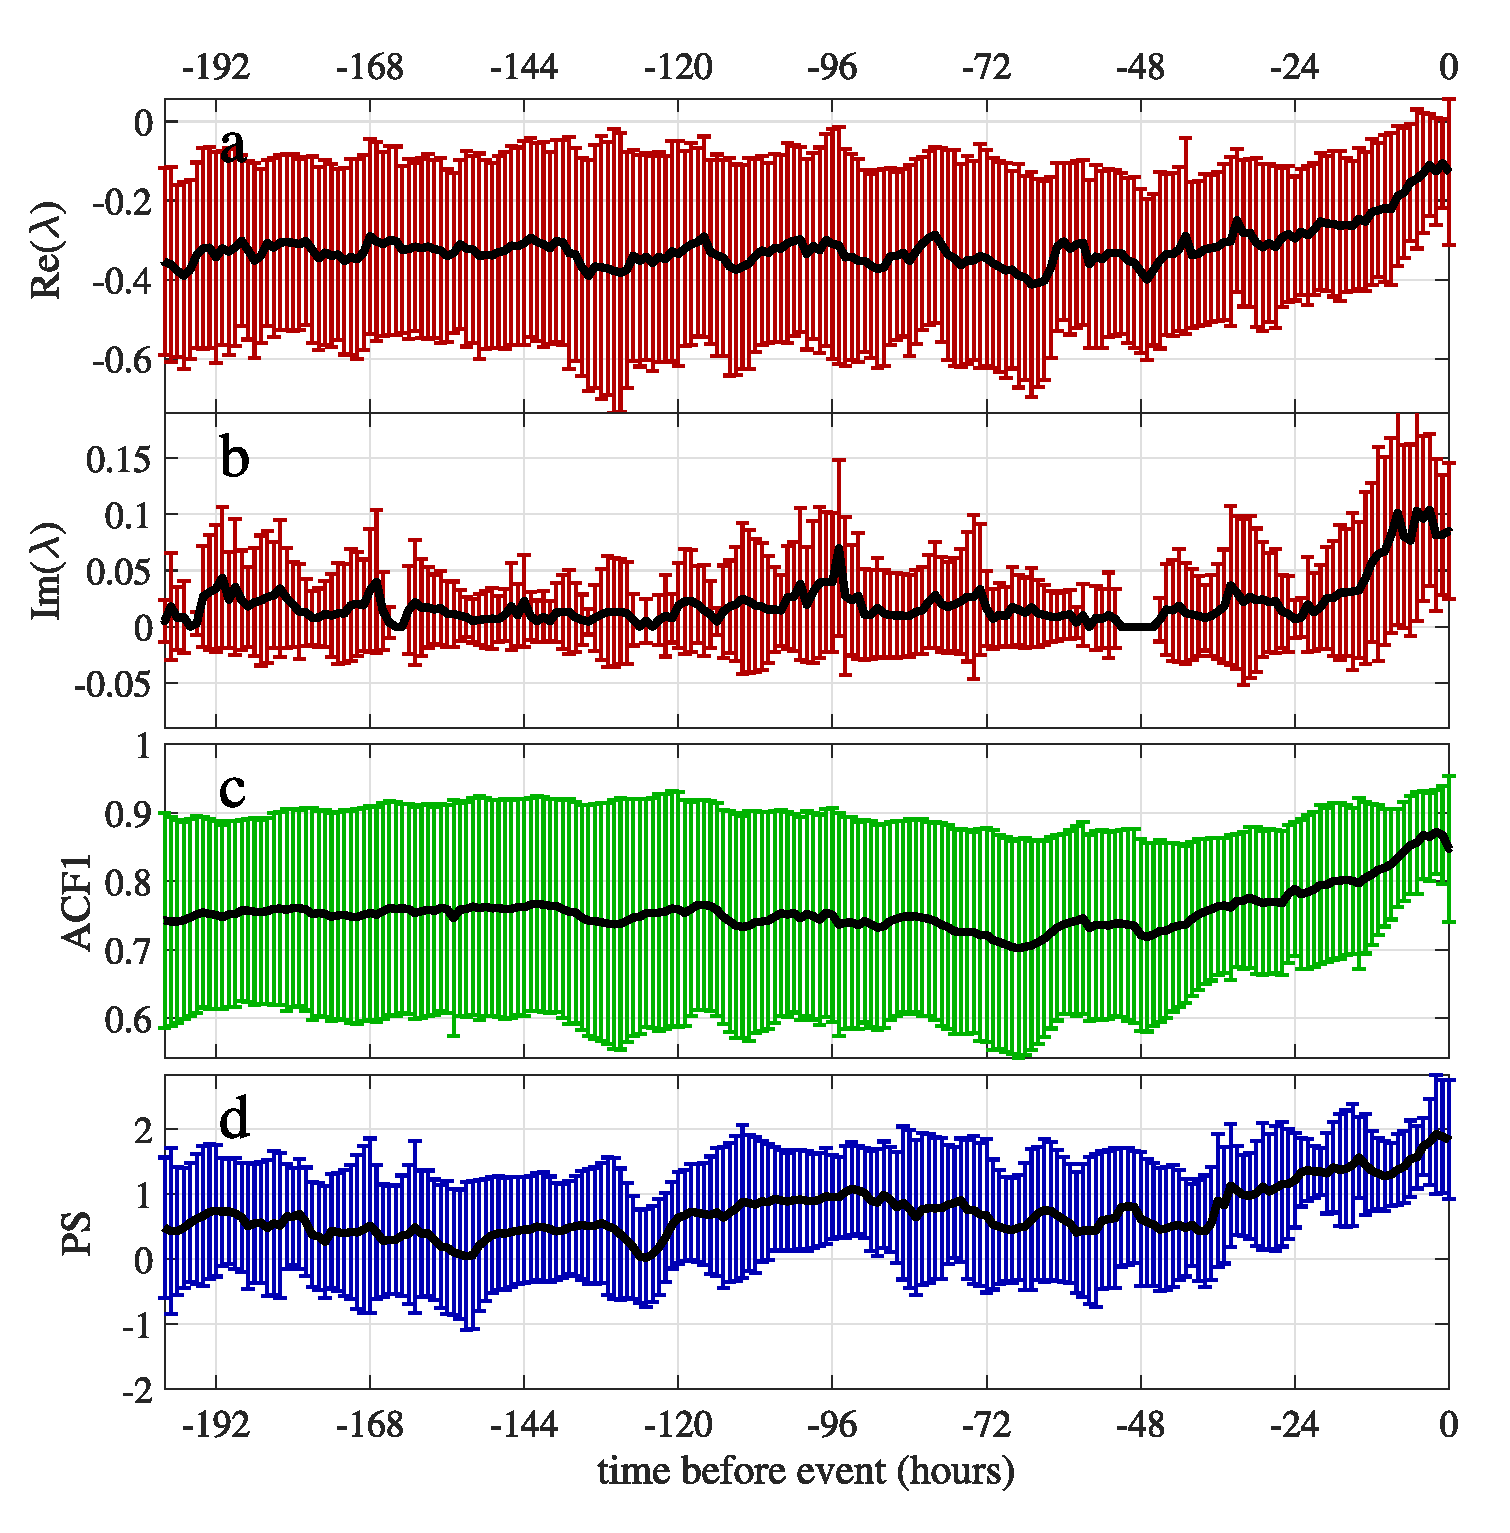
\includegraphics[width = 0.9\textwidth]{indicators_WLandEOF} \caption{\label{fig:TC:indicators_WLandEOF} Multivariate indicator methods applied to sea-level pressure and wind speed data in fourteen tropical cyclones. Mean value shown in black with error bars of one standard deviation over the fourteen series. Panels \textbf{a} and \textbf{b}: the real and imaginary parts of the principal Jacobian eigenvalue calculated in a sliding window of 90 hours. Panels \textbf{c} and \textbf{d}: the ACF1 and PS indicators calculated for the windowed EOF projection using window sizes 90 and 102 hours respectively. For the ACF1 indicator, the sea-level pressure and wind speed variables are weighted $40:60$.}
\end{figure}


\subsection{Weighting sensitivity in EOF techniques}
\label{subsec:TC:2D_SA}

The Jacobian eigenvalues technique takes into account only the covariance between the two variables and is not sensitive to the relative weights of the variables. That is, if the data in one column were changed to different units resulting in values many times larger, the eigenvalues (but not the eigenvectors, which are not studied) would not change. The calculation of EOFs, however, is sensitive to different weighting schemes. By multiplying each variable (each column of the data matrix) by different scalar values, we are able to assign greater or lesser importance to each variable. 

We are therefore able, by visualising the indicator series for a variety of different weighting schemes, to select an optimum weighting in each case. For the data matrix $X$, where the columns of $X$ are the time series variables, we instead use the weighted matrix 
	\begin{equation}
		X_{w} = XW,
	\end{equation}
where, in our case,
	\begin{equation}
		W = \begin{bmatrix}
		p & 0\\
		0 & 1-p
		\end{bmatrix}~,~~~~~p\in [0,1].
	\end{equation}
For $p=0$ the first column of $X$, in our case the sea-level pressure variable, is given no weight and the indicator series is identical to the one-dimensional indicator applied to wind speed alone. Conversely, when $p=1$, only the sea-level pressure is considered. 

\begin{figure}
	\centering
	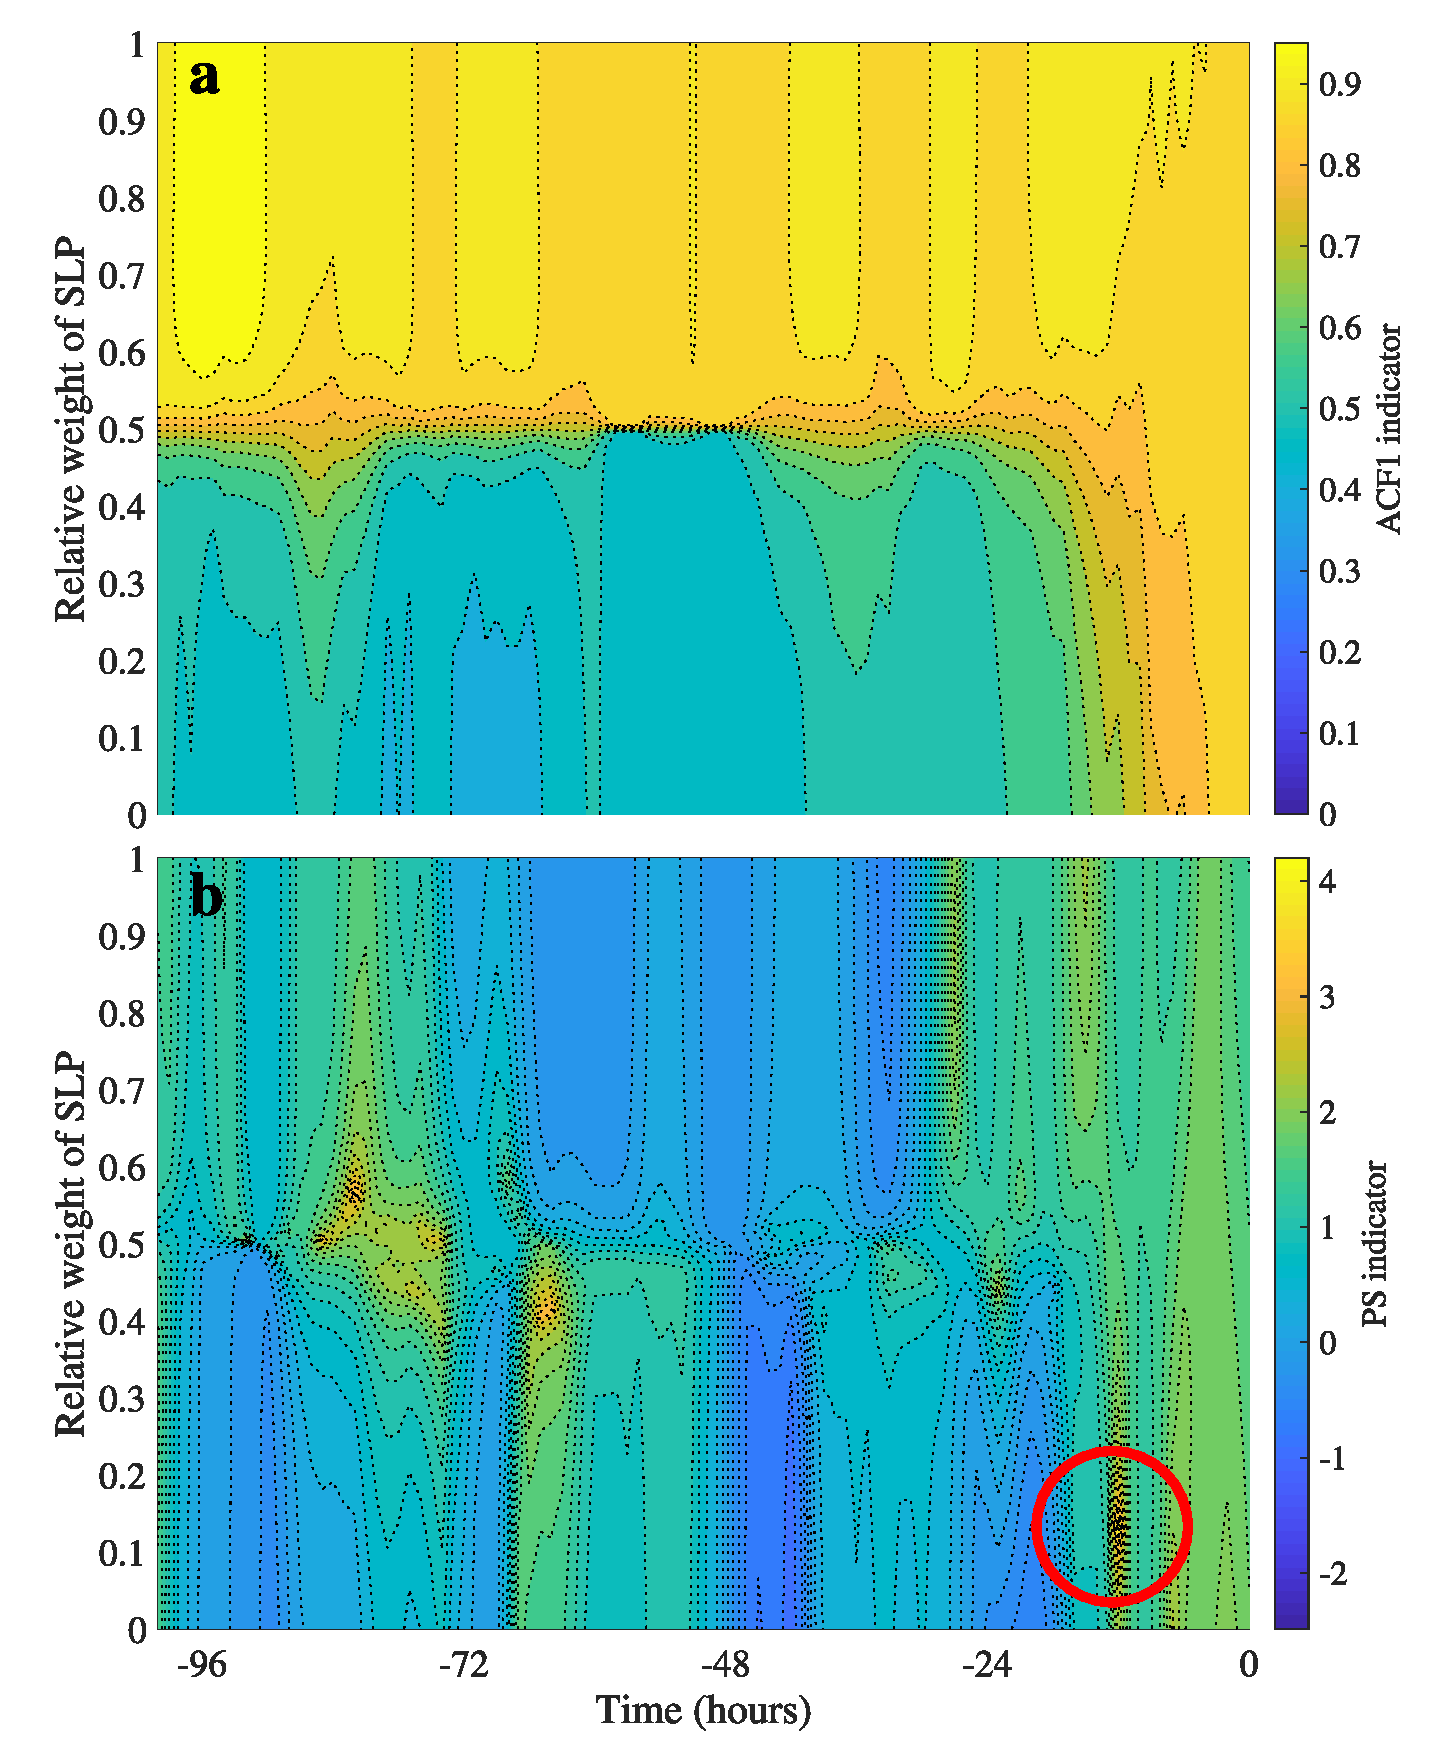
\includegraphics[width=0.9\textwidth]{weightsensitivity_both}\caption{Sensitivity of the ACF1 and PS indicators to different EOF weighting schemes. The widowed EOF projection is found for a range of SLP weighting values from $p=0$ (only wind speed considered) to $p=1$ (only SLP considered) and the ACF1 and PS indicators are calculated (panels \textbf{a} and \textbf{b} respectively). A non-periodic spike in the PS indicator is circled in red. \label{fig:TC:weightSensitivity} }
\end{figure}

The EOF projection is found for a range of values from $p=0$ to $p=1$ and the PS and ACF1 indicators are calculated. The results for the ACF1 indicator and the PS indicator are both shown as contour plots in figure~\ref{fig:TC:weightSensitivity}. We note that, when using the ACF1 indicator, there is a clear difference between $p<0.5$ and $p>0.5$. Weighting the sea-level pressure variable at $0.4$ is effectively equivalent to weighting it zero. Likewise, weighting the SLP variable at $0.6$ is effectively equivalent to weighting it $1$. When SLP is weighted more heavily than wind speed ($p>0.5$) the ACF1 indicator is consistently high and does not provide an EWS, which is already apparent from the ACF1 indicator applied to SLP alone (see figure~\ref{fig:TC:1DindicatorsSLP}b). Using $p<0.5$ there is an increase in the indicator prior to the event, as in figure~\ref{fig:TC:1DindicatorsWS}b, and this rise appears earlier as the relative weight of the SLP variable increases, up to the complete qualitative change at $p=0.5$. It appears that choosing a value $p=0.4$ would provide the best EWS in this case. 

For the PS indicator, the picture is more similar for different weighting schemes. The contour plot is complicated by a few unexplained spikes with much higher indicator values than the surrounding points. For example, for the specific weighting $p=0.15$ there occurs a non-periodic spike at -12 hours where the PS indicator is greater than $3$, this spike is circled in red in figure~\ref{fig:TC:weightSensitivity}. It is possible that this approach could be used to determine specific weightings to avoid, based on the presence of spikes, but this would not be practical without prior knowledge of the spikes' distribution.


\section[Spatially separated data]{Early warning signals for tropical cyclones using spatially distributed data}
\label{sec:TC:field_data}

Here we make an attempt to use the one-dimensional EWS indicators applied to multiple time series data distributed over a geographic area. We investigate the spatial variation in the indicator series, potentially with a view towards detecting a spatial pattern which may provide a warning of the arrival of the tropical cyclone. {\Red{The results presented in this section have previously been published in \cite{prettyman2019}.}}


\subsection{Method}
\label{subsec:TC:fieldmethod}

For this analysis nine separate tropical cyclone events were selected (see section~\ref{subsec:TC:data:HadISD}) which are described in table~\ref{tab:TC:9hurricanes}. {\Red{These events were selected due to an availability of data at several stations within 200~km of the landfall location of the hurricane, which gives between $21$ and $48$ stations depending on the hurricane (see column ``\# stations'' in table~\ref{tab:TC:9hurricanes}, page~\pageref{tab:TC:9hurricanes}).}} The sea-level pressure data were obtained from each station within this radius in a period of twenty days before landfall, and stations were disregarded where more than ten points were missing during this period. The data from the remaining stations were linearly interpolated onto the entire one-hourly time series.

For each of the nine hurricanes, we take the sea level pressure data from all available stations in the region supplied by the HadISD 2017 dataset. We then calculate the PS indicator series for each pressure dataset and asses the slope of that indicator series, using the Mann-Kendall coefficient (see equation~\ref{eqn:TC:MannKendall}), in a window of approximately 30 hours before the hurricane enters the region. If the behaviour here is similar to the behaviour of the mean of the PS indicator applied to the individual sea level pressure series (figure~\ref{fig:TC:1DindicatorsSLP}d), we would expect that an upward trend in the indicator (i.e. a high positive value of the Mann-Kendall coefficient) will be detectable for each location within 30-hours travelling time of the hurricane. We expect that the slope of the PS indicator series would be high at points where the hurricane is very close and lower at points further from the point where the hurricane enters the region. 

The window size used in the calculation of the PS indicator series, and the length of the window in which the Mann-Kendall coefficient is evaluated, are determined for each hurricane through a sensitivity analysis similarly to the process described in section~\ref{subsec:TC:1D_SA}, which is presented in figure~\ref{fig:TC:3by3_sensitivity}. In these contour plots, the mean is not taken over the indicator series for all tropical cyclones, as in section~\ref{subsec:TC:1D_SA}, but rather an individual contour plot is presented for each cyclone in which the mean is taken over all the stations in that region. We see that there is again a significant qualitative change as the window size increases over 100 hours. We note that the increase in the indicator is usually seen in a 30-50 hour window before the event, which is consistent with our expectations based on previous analysis.

As a result of the sensitivity analysis in figure~\ref{fig:TC:3by3_sensitivity} we take the decision to measure the Mann-Kendall coefficient of the indicator series (for the time series at each spatial location, separately) in a 30-50 hour window before a time $T_{\text{entry}}$, which is when the cyclone enters the region under study: that is the time at which the minimum pressure is attained at the first spatial location on the cyclone's path. We expect to see a high coefficient value (i.e. a large increase in the indicator) at locations close to the entry point.
	\begin{figure}
		\centering
		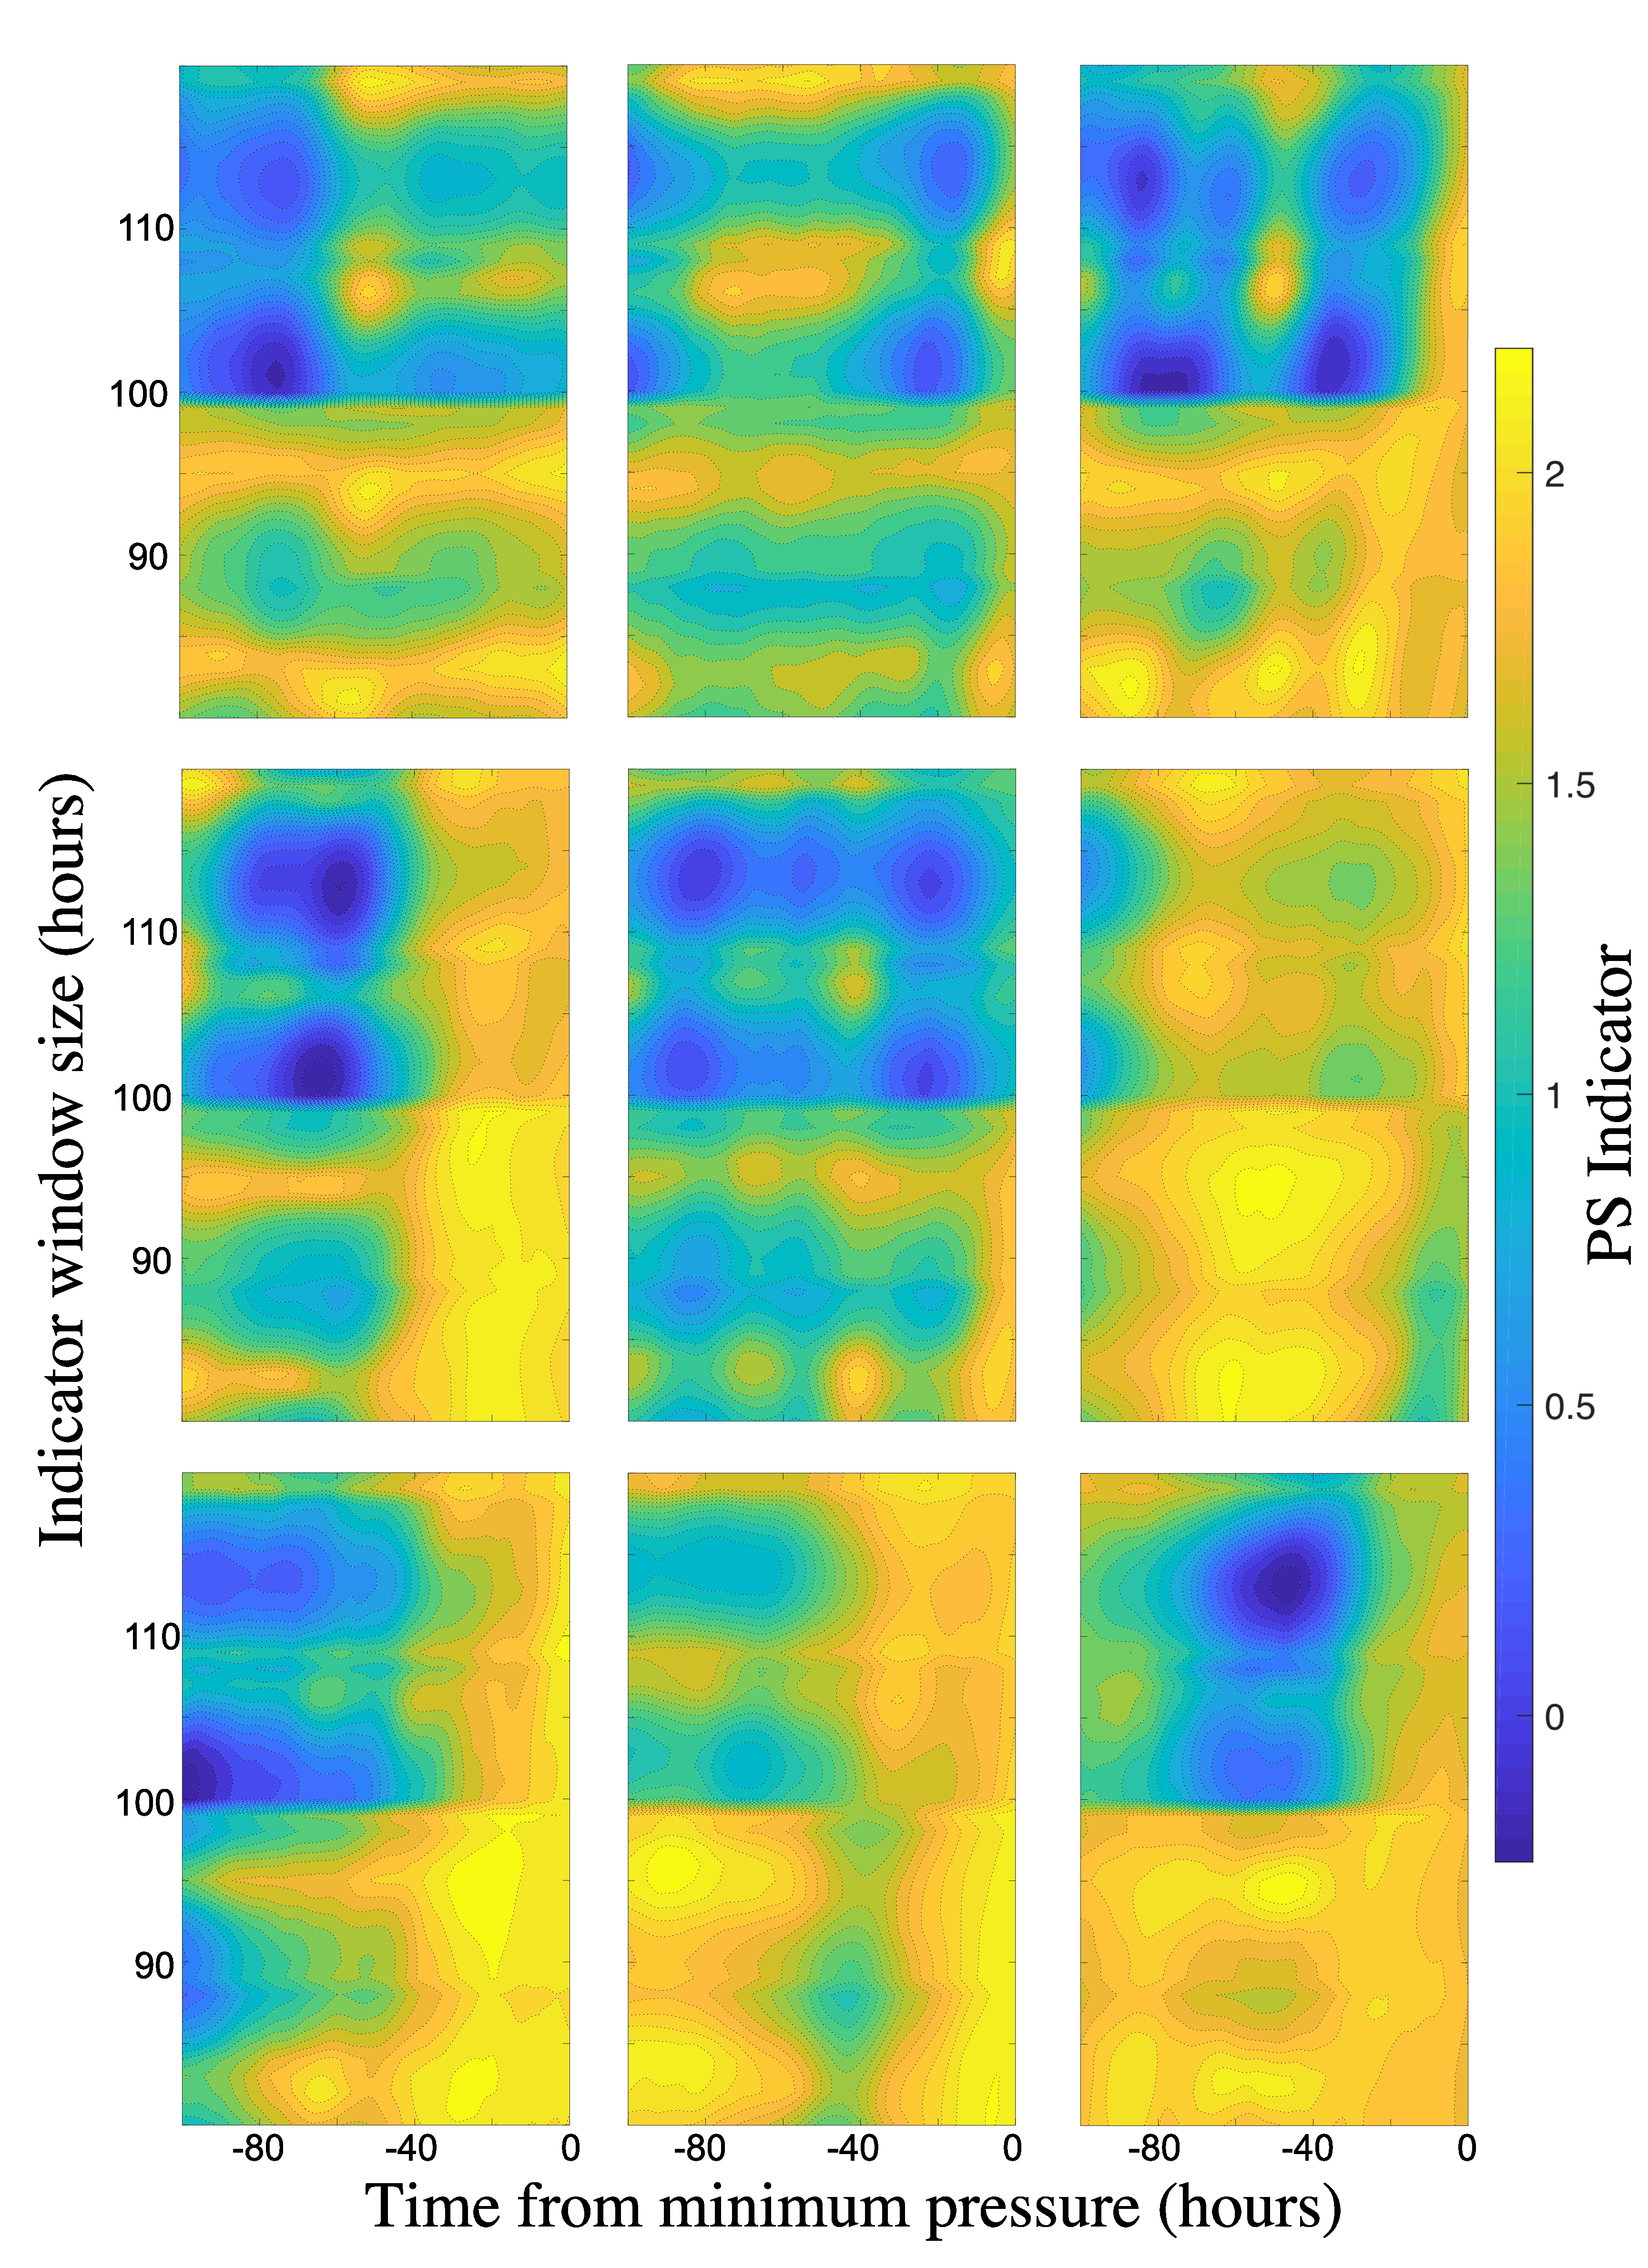
\includegraphics[width = 0.9\textwidth]{Sensitivity3x3}
		\caption{\label{fig:TC:3by3_sensitivity} Contour plots showing the sensitivity of the PS indicator to the window size. Reading left to right the plots show the results for: Andrew (Florida); Andrew (Louisiana); Katrina; Wilma; Gustav; Matthew; Harvey; Irma; Nate. In each case, for each window size, the PS indicator is calculated for the sea-level pressure time series given at each station in the landfall region and the mean taken over all of these stations.}
	\end{figure}
Also, according to the sensitivity analysis, we note that the PS indicator is most useful when using a window size which is an odd multiple of six, consistent with the result of the previous sensitivity analysis in section~\ref{subsec:TC:1D_SA}. This is likely due to the 12-hour tidal oscillations in the data. For each cyclone we have chosen an indicator window size of either 90 or 102 points.

\subsection{Results}
\label{subsec:TC:fieldresults}

\begin{figure}
	\centering
	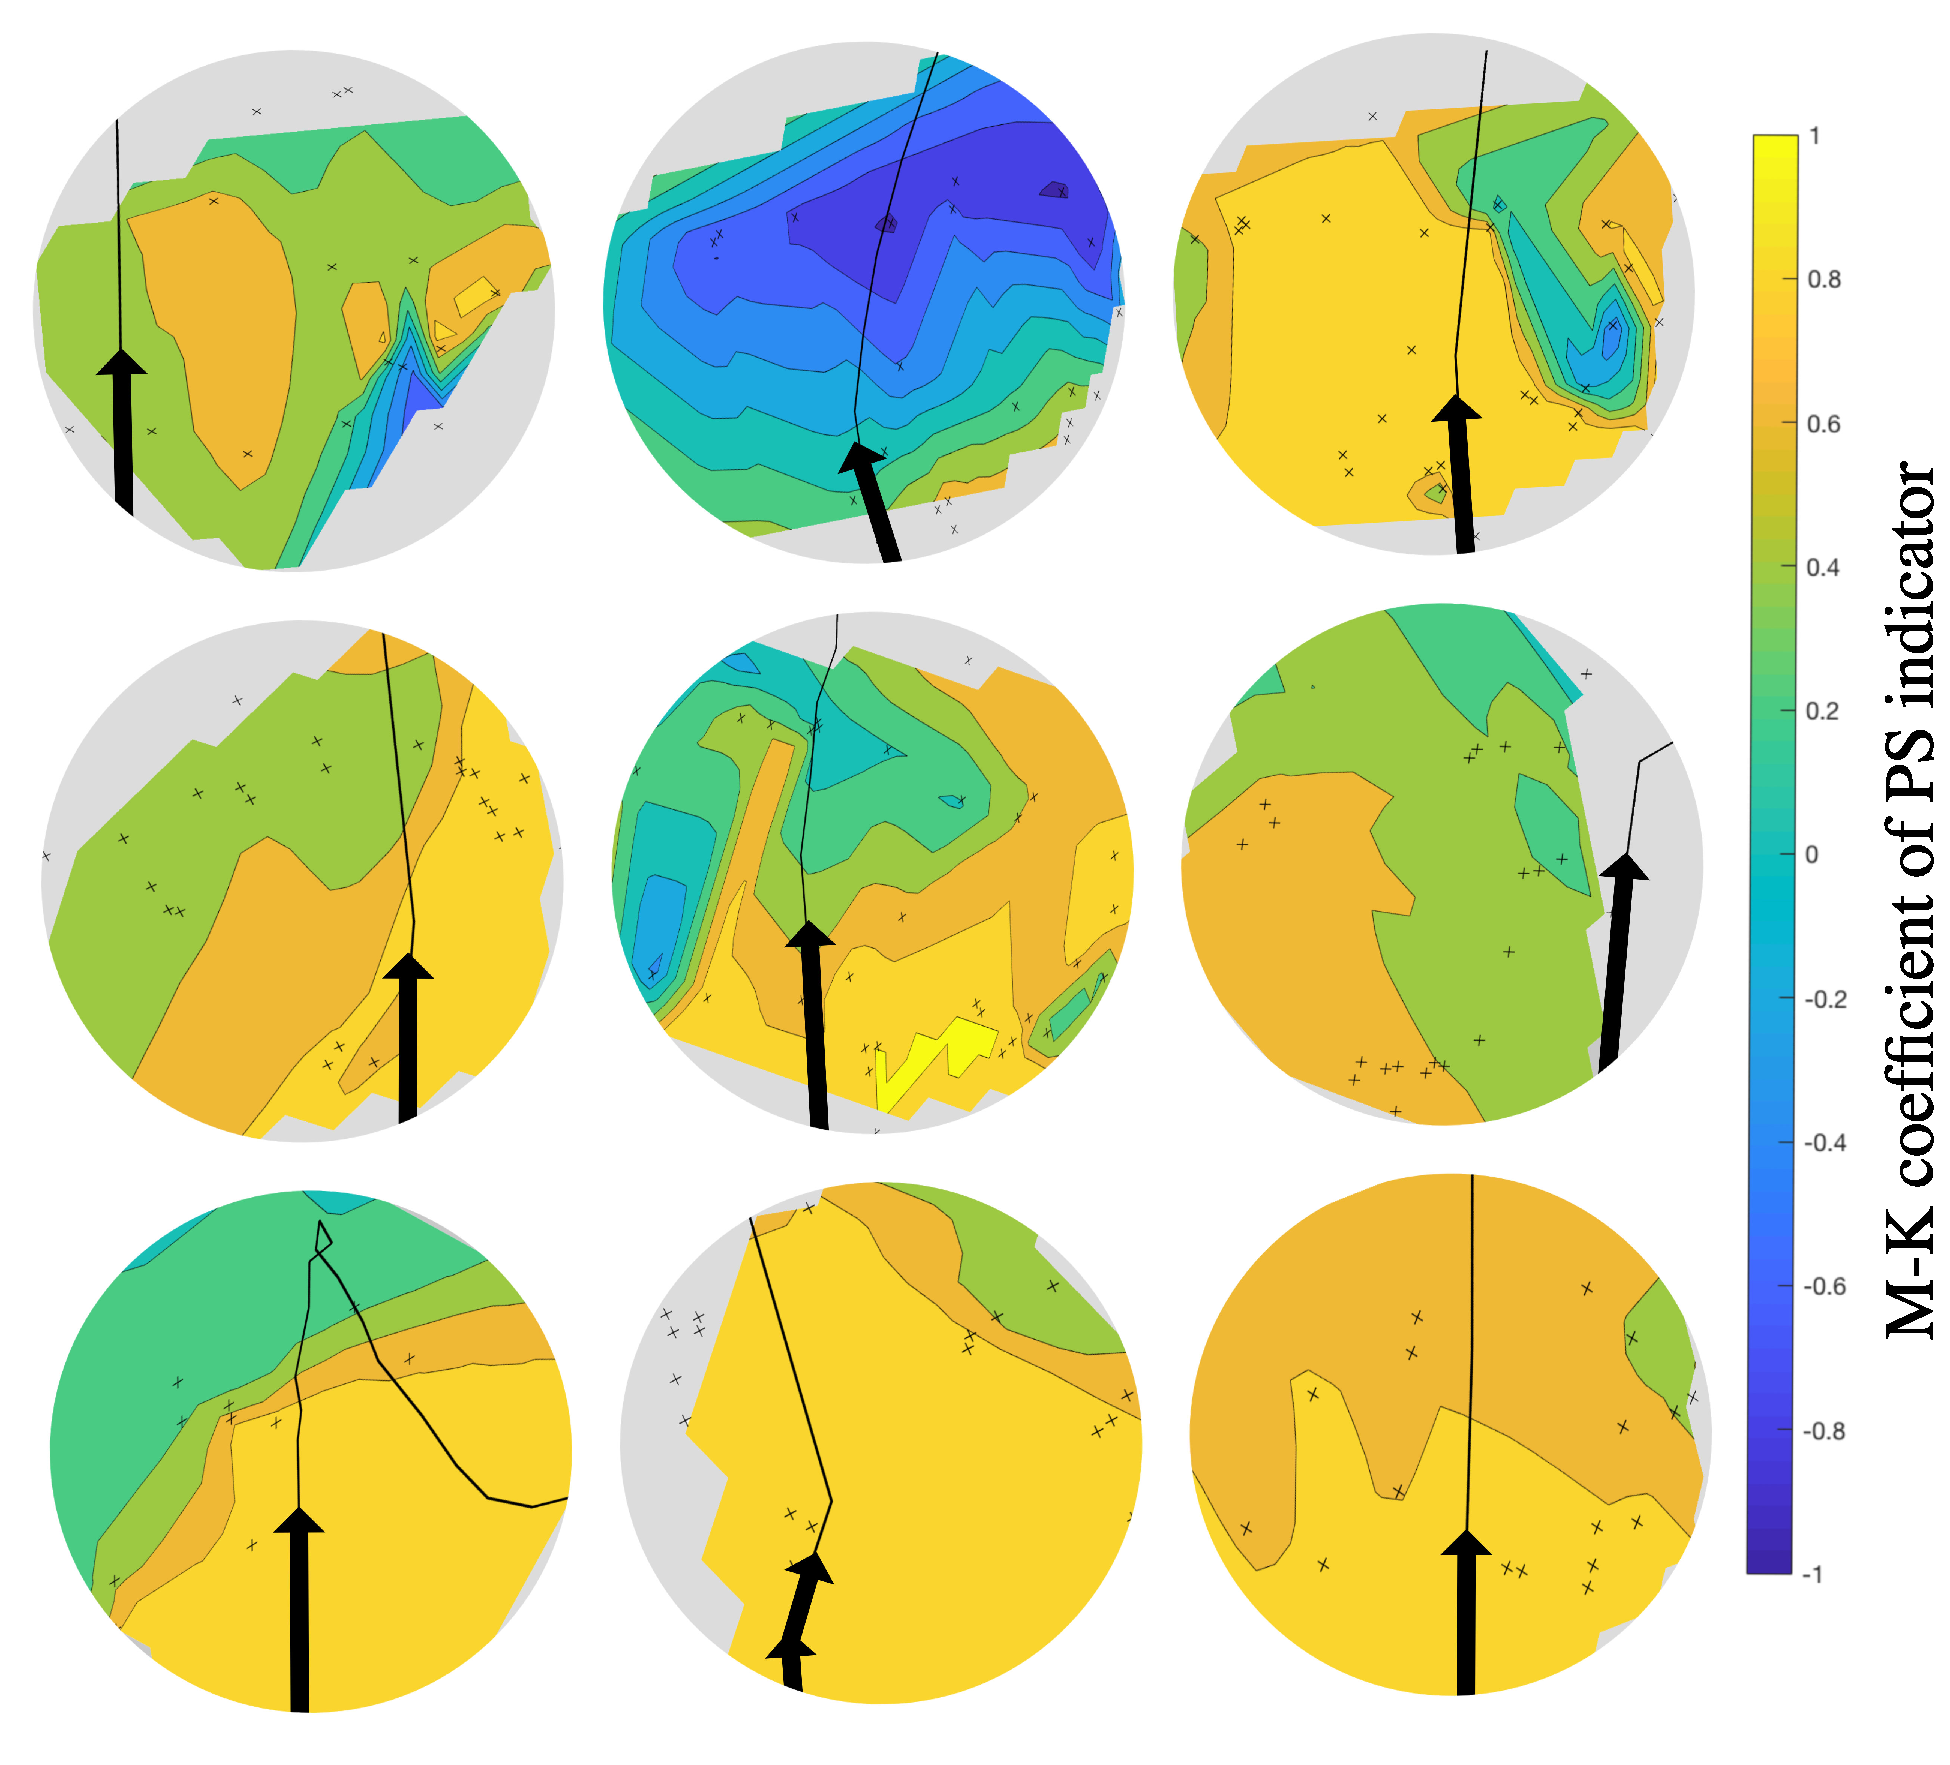
\includegraphics[width = 0.9\textwidth]{Contour3x3}
	\caption{Contour plots of PS indicator gradient for nine Atlantic hurricanes on the Caribbean and Florida coastlines of the USA. left to right: Andrew (Florida); Andrew (Louisiana); Katrina; Wilma; Gustav; Matthew; Harvey; Irma; Nate. In each case, the slope of the PS indicator is evaluated using the Mann-Kendall coefficient and the value of this coefficient is plotted over the geographic area. Each plot has been rotated so that the hurricane track is moving from the bottom to the top of the image (shown by the black line, direction indicated by thick black arrow). The locations of the weather stations are shown by crosses; the grey areas fall outside of the polygon enclosing the weather stations and are therefore not interpolated onto.}
	\label{fig_ContourMapSummary} 
\end{figure}

The value of the Mann-Kendall coefficient of the PS indicator is plotted as a filled contour plot over the geographic area. In figure~\ref{fig_ContourMapSummary} we present a summary of the results: in each case, the contour map is rotated so that the forward path of the Hurricane is moving from the bottom to the top of the image. Hurricane tracks, obtained from the NOAA HURDAT2 dataset (see section~\ref{subsec:TC:data:HURDAT}) are shown by the black line. We are generally able to see a movement of the hurricane from areas with a high value of the Mann-Kendall coefficient, towards areas with lower value, as we expect. Whilst this doesn't provide a useful EWS, it is clear that the PS indicator provides a more robust EWS when applied to many time series in a region than when applied to individual series, as in figure~\ref{fig:TC:1DindicatorsSLP}d.






\section[A tropical cyclone model]{A model of sea-level pressure in tropical cyclones}
\label{sec:TC:Model}

{\Red{
In this section we develop a model of the pressure profile of an approaching tropical cyclone, based on the simple deterministic model developed by \cite{holland1980}. We aim to add a stochastic component to the model which we will parametrise using the early warning signals from the PS and ACF1 indicators obtained in section~\ref{sec:TC:1Dtechniques}. It is expected that by using the values of the PS and ACF1 indicators, obtained from our study of actual sea-level pressure data, we will be able to recreate the stochastic component of the sea-level pressure as observed in the actual data and, by adding this into the model, obtain something that looks like a genuine sea level pressure signal. If we are able to parametrise our stochastic model in this way it will be a verification of effectiveness of the PS indicator in obtaining useful information about the system. {\Red{This model has been presented in \cite{prettyman2019}.}}

We emphasise that it is with this goal of verifying the effectiveness of our techniques in mind that we proceed to develop the model of a tropical cyclone including a stochastic component. It is not with a view towards using the model for practical modelling or forecasting purposes, although this may be interesting subject for future work to be achieved by further developing the model presented here.
}}

\subsubsection{The deterministic model}

\citet{holland1980} presents a simple analytic model of the pressure profile $p$ of a hurricane:
	\begin{equation}
		p(r) = p_c + (p_n-p_c)\exp\left( \frac{-A}{r^B} \right),
	\label{eqn:TC:hollandmodel}
	\end{equation} 
where $r$ is the radial distance from the centre of the hurricane, $p_c$ and $p_n$ are the central and ambient pressures, $A$ and $B$ are parameters to be determined by fitting to observed data. \cite{holland1980} fits the model to three Australian hurricanes: Tracy (December 1974), Joan (December 1975) and Kerry (February 1979). The values of parameters $A$ and $B$ are obtained by fitting to sparse observations, particularly the observations of maximum wind speed $V_m$ given by
	\begin{equation}
		V_m = \left(\frac{B(p_n-p_c)}{\rho e}\right)^{1/2}\,,
		\label{eqn:TC:model:V_m}
	\end{equation} 
and occurring at a radius $R_w = A^{1/B}$. 

Here we present a similar model modified so that the pressure is modelled at a fixed point in space as a function of time, rather than a profile modelled at a fixed time as a function of the distance from the hurricane centre. We are therefore able to model the effect on sea level pressure (at a weather station, for example) of an approaching hurricane. 
We use the values $A=40$ and $B=1$ which are obtained by fitting to Hurricane Katrina (2005) at peak intensity. We consider a fixed point at distance~$d(t)$ from the hurricane centre at time~$t$. In equation~\ref{eqn:TC:hollandmodel}, we replace $r$ by $d(t)$ to introduce a time dependence. We assume the hurricane moves in a straight line towards the fixed point with a speed of $v(t)$~kmph, in which case we have $d(t) = \int_0^t v(s) ds$. For this model, a constant velocity will suffice: 18~kmph is obtained by taking a mean of the nine tropical cyclones studied in section~\ref{sec:TC:field_data} using the HURDAT2 data (see section~\ref{subsec:TC:data:HURDAT}). We in fact use a constant velocity sampled uniformly from the range~$[16,20]$ so that not all implementations of the model are identical. The ambient pressure, $p_n$, is given by 
	\begin{equation}
		p_n(t) = 1016 + 5\eta_1 + 1.6\sin\left(\frac{2\pi t}{12} + K\right),
	\label{eqn:TC:ambientpressure}
	\end{equation} 
where the sine wave models the 12-hourly tidal oscillations and $K$ is a random offset chosen uniformly in the range {\Red{$[0,2\pi]$}}. The central pressure is given by $p_c = 950+10\eta_2$. Values $\eta_1$ and $\eta_2$ are sampled from a standard normal distribution. The reason for the inclusion of $\eta_1$, $\eta_2$ and the random offset $K$ is that we may wish to run the model multiple times and take the mean of statistics over those simulations to obtain an ensemble estimate. For this purpose, we would not want all of the sine wave components to be aligned, nor for all the models to have exactly the same initial parameters.

\subsubsection{The stochastic component}

{\Red{
We observe, in the HURDAT2 sea-level pressure data, that fast-scale noisy fluctuations occur in the times series on top of the large-scale dynamics and the 12-hour tidal oscillations. These fast-scale fluctuations are not included in equation~\ref{eqn:TC:hollandmodel}, but we wish to model them as an additional stochastic component. 
}}

There is also a need to model the increasing memory in the pressure signal, shown to exist using the PS indicator. We therefore add a noise signal to the output in which the power spectrum scaling exponent $\alpha$ increases over time. The maximum value of $\alpha$ is greater for points closer to the cyclone track, and the time at which the maximum value is reached is the time at which the closest approach occurs, which we call $T_{\min}$. We have used values such that $\alpha=0.4$ for $t<t_{\min}-50$ (more than fifty hours before the minimum approach distance is reached). In the 50-hour window, the value of $\alpha$ increases linearly from the background value of $0.4$ to a higher value $\alpha_0$. $\alpha_0$ takes the value 2 in cases where the hurricane path passes directly over the grid-point in question (an approach distance of zero) and decreases linearly with increasing distance from the cyclone track, to a minimum value of $0.4$ for grid-points more than 200km distant.

The part of the noise signal with increasing $\alpha$ value is made by concatenating 10 sub-series, each of length 1000 and with a higher $\alpha$ value than the last (covering the range $[0.4, \alpha_0]$), then sampling with an interval size chosen to give a series of the desired length. All of the noise signals in the model are generated by the method detailed by \citet{kasdin1995}.

We therefore have the model:
	\begin{equation}
		p(d(t)) = p_c + (p_n(t)-p_c)\exp\left( \frac{-A}{d(t)^B} \right) + \eta_t,
	\label{eqn:TC:OurOwnModel}
	\end{equation} 
where $d(t)$ is the distance to the centre of the hurricane at time $t$, $p_c$ is the central pressure, $p_n(t)$ is the ambient pressure at time $t$ given by equation \ref{eqn:TC:ambientpressure}, $A=40$ and $B=1$ are fitted parameters, and $\eta_t$ is a noise term with changing power spectrum scaling exponent as described above. For every point on a spatial grid we are able to calculate the distance $d(t)$ using simple geometry (we model the hurricane as moving in a straight line for simplicity), generate the noise series $\eta$ and then calculate the pressure at that point using equation \ref{eqn:TC:OurOwnModel}. 

We model sea-level pressure at a single point in space which is approached by a hurricane passing by at a distance of 20km, the model uses a time-step of 0.05 hours and 100 implementations are evaluated. We then calculate the ACF1 and PS indicators in a 100-hour sliding window in order to compare them with the results in figure~\ref{fig:TC:1DindicatorsSLP}. The result is shown in figure~\ref{fig_model100}. We see that the ACF1 and PS indicators behave similarly to the result from the real sea-level pressure data, and the pressure series itself also looks reasonable. 

\begin{figure}
	\centering
	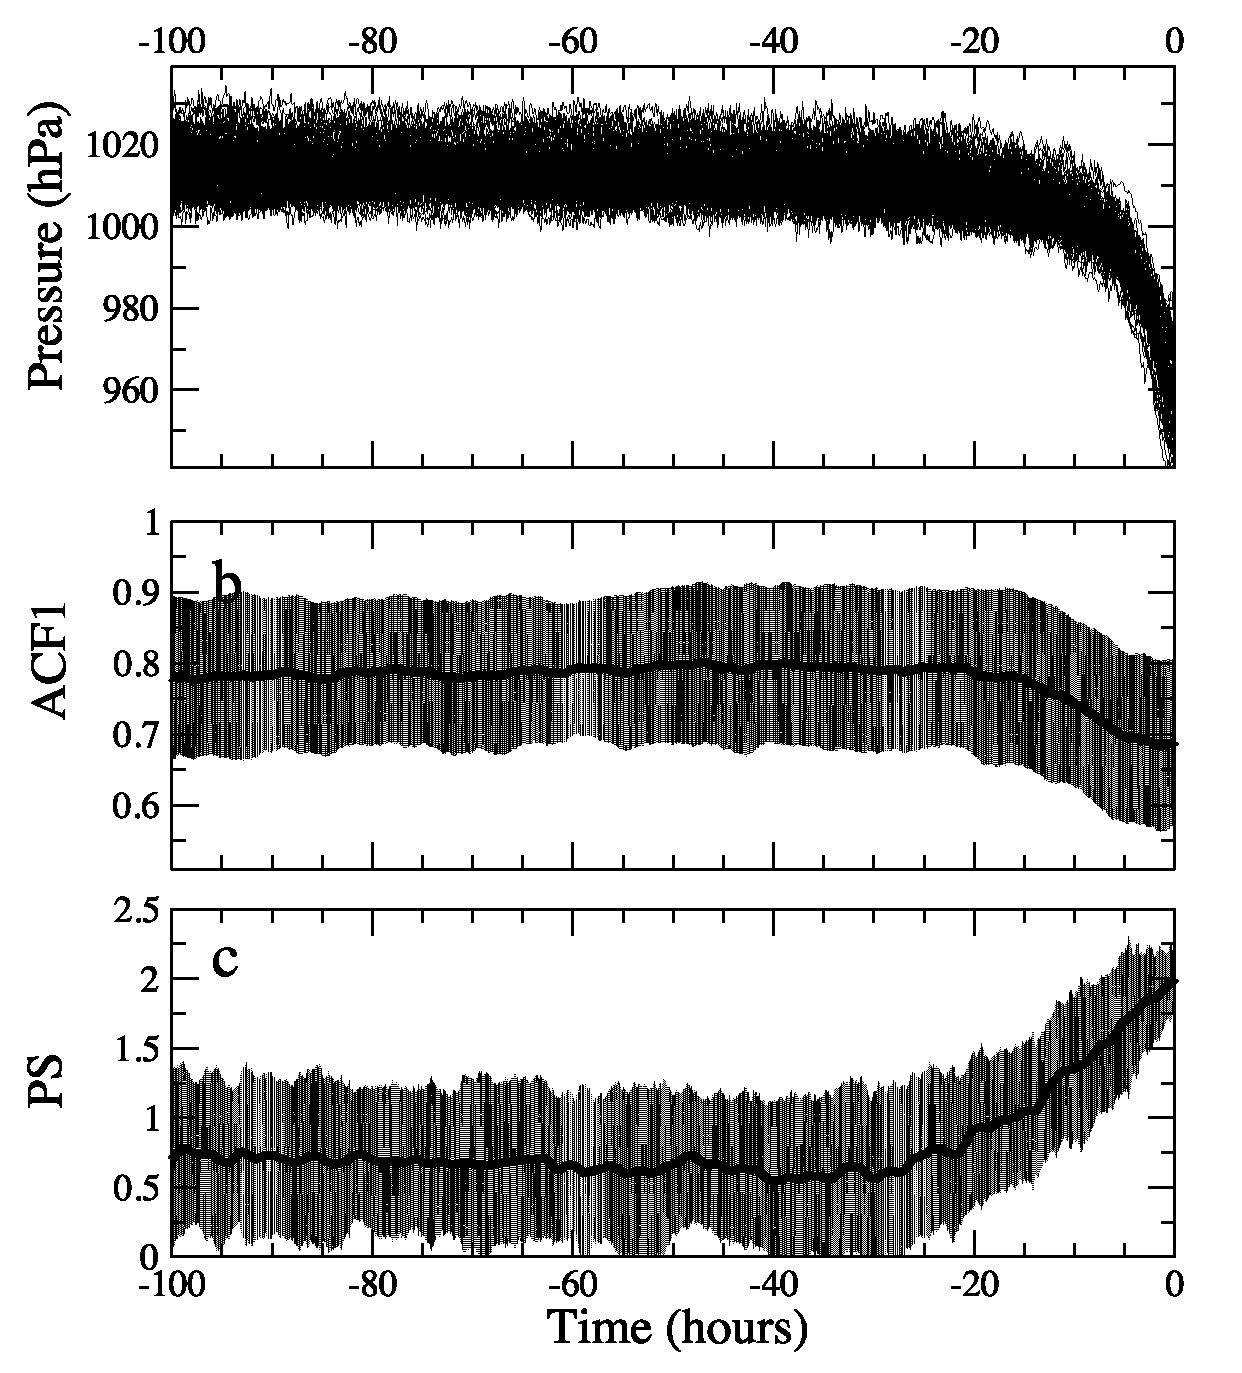
\includegraphics[width = 0.9\columnwidth]{simpleModel100}\caption{\label{fig_model100} Model data (see equation~\ref{eqn:TC:OurOwnModel}) and its EWS indicators. Top panel: 100 instances of the tropical cyclone model. Middle panel: the mean ACF1 indicator. Bottom panel: the mean PS indicator, shown with error bars of one standard deviation.}
\end{figure}

The model is then evaluated with a time-step of 0.05 hours at 100 points in a ten-by-ten grid with 40km spatial separation between points (giving a square of side 360km). The hurricane is modelled as travelling from ‘south' to ‘north' from 400 hours before reaching the bottom of the grid up to the point where it reaches the top of grid. The PS indicator of the pressure signal for each grid-point is calculated in a 100-hour sliding window (of 20,000 points). We then calculate the PS indicator slope, evaluated using the Mann-Kendall coefficient, in the exact same way as shown in the previous section (figure~\ref{fig_ContourMapSummary}), in the 30-hour window before the hurricane reaches the bottom of the grid. Figure~\ref{fig_tenModelRuns} shows the mean over ten such evaluations for ten separate runs of the model. We see that the pattern is consistent with our expectations and also with the general pattern of the analysis of real data in figure~\ref{fig_ContourMapSummary}. This confirms our understanding of the hurricane statistics.

\begin{figure}
	\centering
	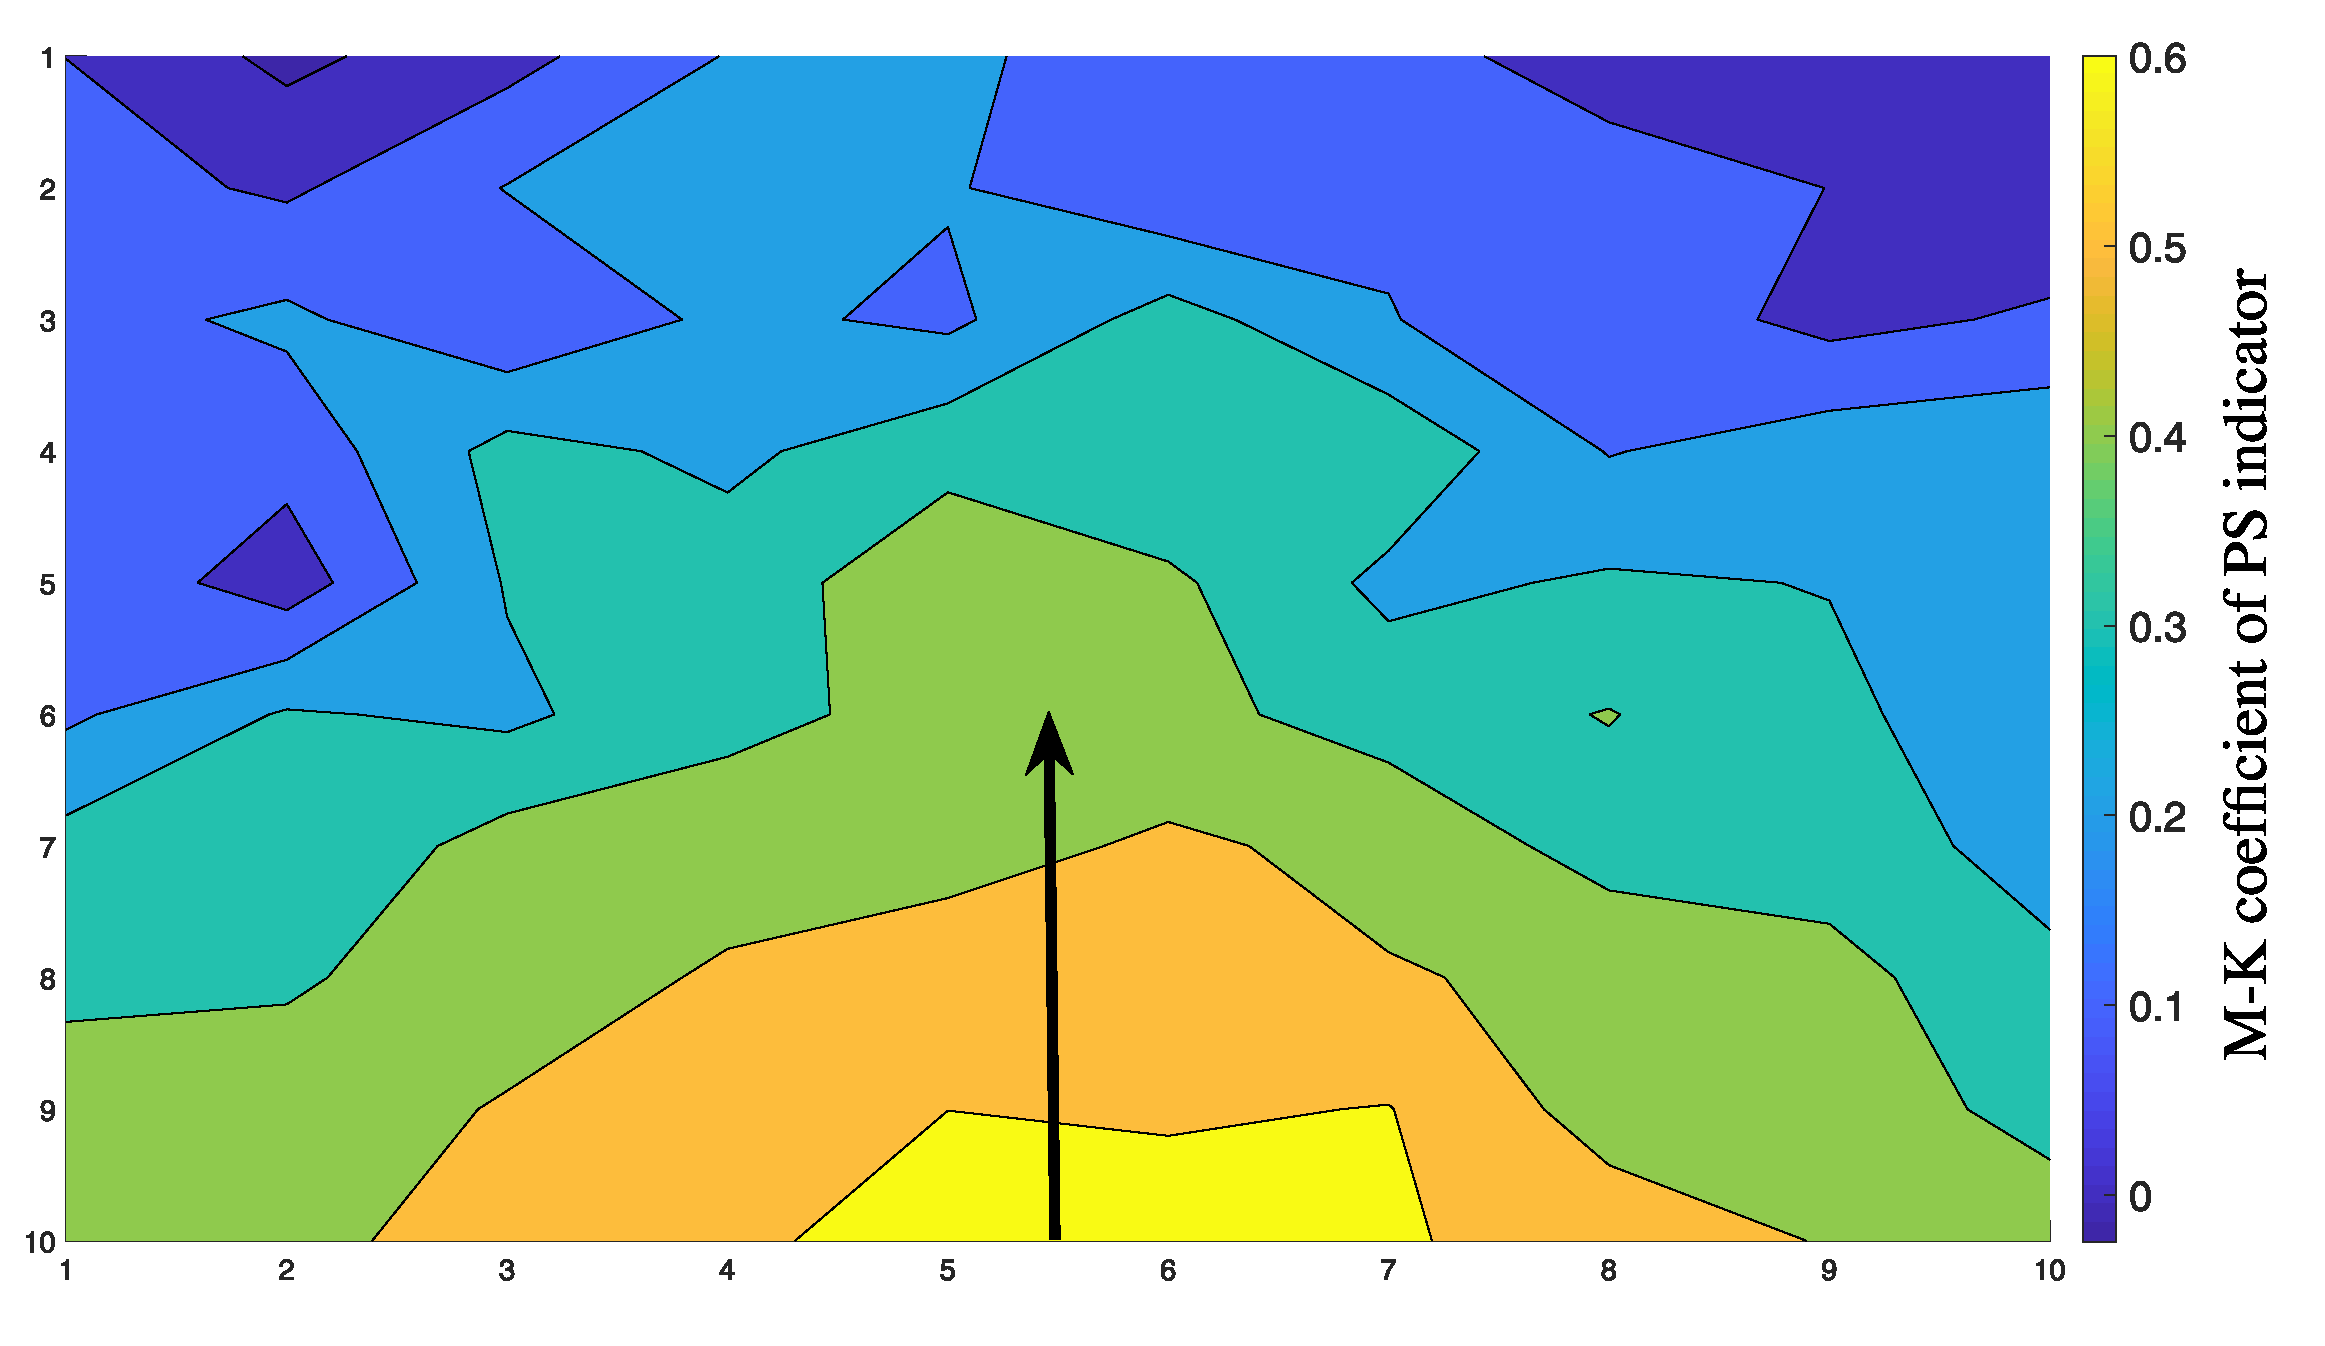
\includegraphics[width = 0.9\textwidth]{07_tenModelRuns}\caption{\label{fig_tenModelRuns} The mean of the PS indicator slope (evaluated using the Mann-Kendall coefficient) over ten realisations of the hurricane model. The slope is evaluated for the PS indicator of the pressure signal at each of 100 grid points with 20km spacing, in a 30-hour window before the modelled hurricane reaches the bottom of the image. The motion of the hurricane is shown by the black arrow.}
\end{figure}


\section{Discussion}\label{sec:TC:discussion}

We have applied the tipping point indicators introduced in chapters~\ref{chap:1D} and~\ref{chap:2D} to the meteorological variables measured in the vicinity on an approaching tropical cyclone. When applied to the sea-level pressure data, the ACF1 and DFA indicators do not appear to provide an EWS. {\Red{\label{pageref:TC:exaggeration} However, looking at the mean over the ensemble of fourteen cases, the PS indicator appears to begin to increase around 48 hours before the lowest pressure, although this increase is not significant when considering the error in the signal. This is about the same point ($-48$ hours) that the decreasing trend in pressure becomes visible, suggesting that it may be able to provide a detectable EWS in this context, if longer time series and larger ensembles were available.}} The methods used to incorporate wind speed data into the analysis besides sea-level pressure have not appeared to yield any improvement, this is possibly due to the two variables being closely correlated. 

We have also attempted to increase the robustness of the results provided by the PS indicator by including data from many points in a close geographical region. This has not produced a reliable early warning signal but it has allowed us to visualise an approaching storm by plotting the strength of the increasing trend in the PS indicator over the region. We have therefore confirmed that in this specific system the PS indicator increases consistently prior to and during the tipping event, which is not a bifurcational tipping, whilst the DFA indicator shows no change (see section~\ref{sec:TC:1Dtechniques}). {\Red{\label{pageref:TC:scaling_comment} This is not unexpected since claims that the DFA and PS scaling exponents are linearly related \citep{heneghan2000} are assuming power-law scaling of the power spectrum and DFA segment sizes, whereas we are estimating the PS exponent even in the absence of power-law scaling, as justified by the analysis in section~\ref{subsec:1D:Exponents_as_EWS:nopowerlawsacaling} (page~\pageref{subsec:1D:Exponents_as_EWS:nopowerlawsacaling}). }}

We note that the tropical cyclone example was chosen because it appears to exhibit tipping behaviour whilst not being described, according to our current knowledge, by a bifurcating or state-switching dynamical system often associated with tipping point analysis, therefore presenting the opportunity to apply known methods in a novel system. In future work it will be interesting to apply the PS indicator in other applications where it may be compared to the existing ACF1 and DFA indicators. In particular, the methods applied in section~\ref{sec:TC:field_data} to sea-level pressure data over a geographic area could usefully be applied to the greening and desertification of the Sahara, similarly to the methods presented by \citet{bathiany2013p1} (discussed in section~\ref{sec:2D:ExtensionToGridded}). At the time of writing, model data with sufficient temporal resolution are not available.  

%%%%%%% Cyclogenesis

%schreck2015kelvin
%graf2017objective
%kilroy2017unified
%riehl1950model
%schecter2009hurricane

%maestre2009patch -- vegetation patches for desertification
%lin2010spatial -- 
%kefi2014early
%dakos2011slowing

Another interesting system worth studying with these methods is the formation, rather than the approach, of a tropical cyclone (cyclogenesis) since this is closer to the idea of a complex system undergoing a critical transition \citep{scheffer2009} and therefore a better candidate for tipping point analysis. However, real-life data, at a resolution suitable for tipping point analysis, is not available to our knowledge: it is unlikely that measurements would be taken at the precise location of cyclogenesis. Moreover, there are many different conditions under which cyclogenesis occurs \citep{graf2017objective, kilroy2017unified} and many influencing external factors \citep{schreck2015kelvin}. Since the original aim of this study was to investigate the behaviour of tipping point indicators in a novel system, not necessarily to produce a result useful to practical prediction problems, it was not necessary to select a system with typical bifurcational tipping point dynamics. Rather, the availability of data was the primary concern. A future project, however, could apply tipping point indicators to data from cyclogenesis models, such as the model presented in \citet{schecter2009hurricane} which shows an ordered hurricane forming from a turbulent initial state, producing an image resembling models of tipping points in vegetation coverage \citep{dakos2011slowing, kefi2014early} in which early warning signals have been detected.

We have also presented a simple model of an approaching tropical cyclone parametrised using observed trends in tipping point indicators. {\Red{We suggest that the nature of the noise present in this model is similar to the noise found in a real sea-level pressure signal since we have used our analyses of real sea level pressure time series in the vicinities of tropical cyclones to parametrise the stochastic component of the model. }}
%!TEX root = ../thesis.tex
%************************* Final Chapter ***************

\chapter{Conclusions}
\label{chap:Conc}

\graphicspath{{Chap_Conclusion/Figs/}}
	
	In this thesis we have presented and examined a number of methods related to finding Early Warning Signals for tipping points in dynamical systems. The methods we have chosen for study are mostly extensions of the ``fingerprinting'' technique of \cite{held2004} in which the value of a certain `indicator' is tracked over time and a change in this value is supposed to be a warning of a tipping point. Thus, the indicator value, plotted as a function of time, is the early warning \emph{signal}. In general, it is not the actual value that matters but the change in the value.
	
	In chapter~\ref{chap:1D} we have studied the uses of the ACF1 indicator which is common in the literature, the DFA indicator which was developed by \cite{livina2007}, and the PS indicator which is a result of this work \citep{prettyman2018,prettyman2019}. All of these indicators have been found, in certain systems containing tipping points, to provide useful early warning signals, although in these cases the data from which the EWS is obtained is a one-dimension time series. A pressing problem in the field of early warning signals is, therefore, to find methods which can be applied to higher-dimensional systems such as those presented by \cite{williamson2015} and \cite{williamson2016} and the analysis of spatial correlations by \cite{bathiany2013p2} or \cite{kefi2014early}. In the climate science in particular the dynamical systems under investigation are often extremely high-dimensional. The methods presented in chapter~\ref{chap:2D} are intended as an important step in this direction, although we restrict our study to two-dimensional systems. The example in chapter~\ref{chap:cyclones}, that of a tropical cyclone, is likewise studied in the context of one- or two-dimensional early warning signal techniques, with the one-dimensional time series of sea-level pressure data being studied either alone or in conjunction with a second variable: wind speed. 
	
	In the remainder of this chapter we conclude this thesis by providing comments on the work we have done and extending it, hypothetically, into the future by considering lines of research which may take this thesis as a starting point. We do not attempt to summarise the entire thesis here but concentrate on the most significant results from each of the different paths we have travelled along our journey. 
	
	
	
\section{Comments on the PS indicator}
\label{sec:conc:PScomments}

The power spectrum scaling exponent seems an obvious candidate for an early warning indicator since it is closely related to the lag-1 autocorrelation and the DFA exponent which are already used as indicators. In chapter~\ref{chap:1D} we have introduced the idea of using the periodogram for the estimation of the PS exponent, first binning the fast Fourier transform periodogram to give an even distribution of points on the logarithmic scale. 

We base our understanding of tipping point detection and prediction on the idea of \emph{critical slowing down} (see section~\ref{subsec:1D:Exponents_as_EWS:CriticalSD}, page~\pageref{subsec:1D:Exponents_as_EWS:CriticalSD}), which is assumed to precede a tipping point, and which we have modelled as an AR(1) process. This assumption is used in section~\ref{subsec:1D:Exponents_as_EWS:determining_frequency_range} (page~\pageref{subsec:1D:Exponents_as_EWS:determining_frequency_range}) to determine a suitable range of frequencies in which to estimate the exponent. 

As with the development of the DFA exponent for use as an EWS indicator, the question arises that the PS exponent method may not be suitable when the power spectrum of a particular time series does not exhibit genuine power-law scaling. This objection is dealt with in section~\ref{subsec:1D:Exponents_as_EWS:nopowerlawsacaling} where we investigate the analytic relationship between the PS exponent and the parameter $\mu$ of the AR(1) process for which no real power-law scaling exists for $0<\mu<1$. We find that by estimating the PS exponent $\beta$ anyway, finding a linear best fit to the non-linear power spectrum `crossover' function, the result is a consistent, monotonically increasing value of $\beta$ which can be used as a proxy for increasing critical slowing down, similar to the DFA exponent and the lag-1 autocorrelation. In addition, we find the same thing when we assume the AR(1) parameter $\mu$ is non constant over the time series used to estimate the PS exponent (see section~\ref{subsec:1D:Exponents_as_EWS:PSnonstationary}, page~\pageref{subsec:1D:Exponents_as_EWS:PSnonstationary}), in this case the value of $\beta$ we estimate numerically is consistent with what we predict analytically by integrating the power spectrum of the AR(1) process over the range of $\mu$ values. 

Although this analysis confirms that the PS indicator may, in theory, provide an EWS for tipping points which are characterised by critical slowing down, it does not comment on the suitability of the indicator for tipping points which are \emph{not} so characterised, nor in cases when the critical slowing down cannot be modelled as an AR(1) process (the latter case has not been considered in this thesis). Experimentally, we find that the PS indicator does not provide an EWS for noise-induced tipping, consistent with established results for the ACF1 and DFA indicators. Transitional tipping points may or may not be characterised in this way. A future study may be designed to investigate these transitional tipping points further, and also to apply the PS indicator to examples of rate-induced tipping, which has not been studied here. 

Finally, we find that the estimation of the PS exponent requires a relatively long time series, in comparison to the accurate estimation of the lag-1 autocorrelation, for use as an EWS indicator. Where we consider examples of dynamical systems with genuine bifurcations, particularly the super-critical pitchfork bifurcation which is studied in more depth in section~\ref{subsec:1D:indicatorComparison:PitchforkModel}, we use a window size of only $100$ points for the PS indicator, which is not expected to produce a noticeable EWS, but a slight increasing trend can be often be observed nonetheless in the mean of a large enough ensemble. 

We can conclude that the use of the power spectrum scaling exponent as an EWS indicator is, in most cases, inferior to the well-established use of the simple lag-1 autocorrelation. There are, however, some aspects of this new method which may provide benefits and which could be exploited in future work. In particular, the PS exponent is insensitive to certain trends (although we note that the DFA exponent has already been exploited for this reason) and periodicities, particularly when the frequency of the periodicity lies outside the range of frequencies used for the PS exponent estimation. 

The application of the PS indicator to a two-variable system in chapter~\ref{chap:2D}, and to the tropical cyclone problem in chapter~\ref{chap:cyclones}, did not give much more insight into the PS indicator than the one-dimensional `toy model' examples in chapter~\ref{chap:1D}: once again we find that where the ACF1 indicator provides an EWS, so does the PS indicator, although not as strong nor as clear. When the ACF1 indicator fails to provide an EWS, so does the PS indicator. The exception to this is the application to sea-level pressure in the vicinity of tropical cyclones. In this case we discover that the PS indicator rises slightly before the tipping event, while the ACF1 indicator decreases. This inconsistency is possibly due to the 12-hour periodicity in the data due to tidal fluctuations, which is destroyed by the sudden large drop in pressure at the event time. When this periodicity was removed, using either a sine-wave subtraction or a deseasonalising approach, all EWS indicators became more variable and no clear signal was visible in any — it is likely that by subtracting a periodic function from the entire time series we are actually introducing a periodicity into that part of the time series which is not obviously fluctuating originally. In these situations, where attempting to remove periodicities or trends artificially might introduce biases, it may be useful to further explore the potential of the PS indicator which is insensitive to such artefacts. 


\section{Comments on the use of EOFs for dimension reduction}

In chapter~\ref{chap:2D} we have explored the idea of reducing the dimension of time series data using empirical orthogonal functions, thus allowing the use of established one-dimensional EWS techniques when higher-dimensional data is given. This idea is not original to this thesis and we take for granted that using EOFs to reduce dimensionality will give a better result than arbitrarily choosing to analyse, say, only $x$ coordinates. However, the question arises as to whether the EOF projection is optimal for use with EWS techniques. When attempting to find an EWS in a time series, one is interested in looking for \emph{an increase in variance} or \emph{an increase in autocorrelation}, etc.. But the EOF projection finds the time series with the largest \emph{variance}, not the largest \emph{increase in variance} or the largest \emph{increase in autocorrelation}. 

We have taken a simple, general, discrete-time, two-dimensional system as an example and attempted to discover whether the EOF method is optimal, or even appropriate, for use with EWS techniques. What we have discovered is that the EOF projection (which has maximal variance) is the same as, or very close to, the projection which has maximal \emph{increase in variance}, unless there is very large variance in a stationary part of the system. This result is, we believe, not trivial and serves to justify the use of EOFs in a range of EWS applications. 

An alternative EOF-like method for dimension reduction was also proposed, in which the lag-1 autocorrelation is maximised rather than the variance. We found that there was not a significant benefit to using this approach, even when the EWS indicator used on the resulting one-dimensional time series was the lag-1 autocorrelation itself. This result further justifies the use of the standard EOF method in EWS applications. 

We can conclude, therefore, that the EOF method is well-suited to reducing dimension prior to applying EWS techniques and the previously (to our knowledge) unexamined hypothesis that the maximal variance projection will be useful in an application which seeks to find an \emph{increase in variance}, is true in the cases we have considered. In future work it may be instructive to consider systems in dimensions higher than two and to consider other examples of systems which are generalisable to a wider variety of systems experiencing tipping points. 


\section{Comments on other two-dimensional methods}

In this thesis we have been particularly concerned with the method presented by \cite{williamson2015} (see section~\ref{sec:2D:Williamson}, page~\pageref{sec:2D:Williamson}) which estimates numerically the eigenvalues of the system Jacobian matrix in order to obtain a precursor signal of a bifurcation (for example, the negative-real eigenvalues moving towards a positive-real value). Because of the assumptions made on the dynamical system we view this method as similar to using lag-1 autocorrelation as an EWS based on the assumption of the presence of critical slowing down. We have used this method, therefore, as an example against which we compare the performance of the PS indicator in chapter~\ref{chap:2D}, in a natural extension of the work in chapter~\ref{chap:1D} where the PS and ACF1 indicators were compared directly in one-dimensional time series. 

Our results accurately recreated those of \cite{williamson2015} and we found that the EWS is as good as that produced by the ACF1 indicator coupled with the EOF method for dimension reduction, if one knows which eigenvalue to study and has some prior knowledge of how the EWS will look in the case of each specific system. 

In addition, we investigated a number of techniques for detecting tipping points in multiple time series over a 2D field. We presented a simple technique whereby an EWS indicator is evaluated in every time series over the field simultaneously to build up a heat map of a measure of increase in that indicator over a window of time. We find that the resulting picture of the propagation of a bifurcation point across the field is very clear when using the ACF1 indicator and accurately represents the state of the system at each point in time. 

Many other, similar methods exist in the literature (see \cite{bathiany2013p2}, \cite{kefi2014early}) but these were not studied further here, partly because the geophysical example chosen as a test-bed in chapter~\ref{chap:2D}, that of the approach of a tropical cyclone, did not present a good opportunity for studying these methods due to limited data. A future study which aims to test the PS indicator in other systems could, if the data existed in the correct form, use some of these other methods for a comparison. 





\section{Comments on applications to tropical cyclones}

The study of sea-level pressure data obtained from ground-based weather stations on the trajectory of a tropical cyclone is problematic due to sparse data sources and short time series. We were able to identify fourteen weather stations meeting the criteria of being in the path of a large tropical cyclone and having uninterrupted data at the time of the cyclone\footnote{Weather stations are often damaged during unusually powerful storms.}. In each of these fourteen cases we obtained hourly data, giving us only around $100$ relevant data points (often fewer) since a cyclone will often have progressed from first detection (from a given coastal location) to making landfall within a period of $100$ hours. This is just about the lower limit at which the PS and DFA indicators can be applied to a time series. When attempting to detect an effect which may only be detectable in a period of maybe $48$ hours, but the indicator is calculated in a window of $100$ hours, there will necessarily be a watering-down of the effect on the indicators. For this reason, we have not expected to discover any useful early warning signals, and it surprising that any change in the DFA and PS indicators is observed at all. It is not clear from the plots made of the single-value indicators applied to the sea-level pressure series, but when assessing the sensitivity of the indicators to window size we have presented contour plots, or heat maps, of the indicator value at different times before the cyclone event using different window sizes. In these plots we are able to see that the PS and DFA indicators do show a rising trend around $24$ hours before the tipping point when using larger window sizes (>80 points). This is maybe more noticeable in comparison to the same methods applied using shorter window sizes. It is somewhat surprising that there is any noticeable trend at all, no matter how slight, since the analysis of the PS exponent of the AR(1) process (see section~\ref{subsec:1D:Exponents_as_EWS:PSsensitivity}, page~\pageref{subsec:1D:Exponents_as_EWS:PSsensitivity}) does not suggest that the estimation of the PS exponent from just $100$ points would be at all consistent. It will be necessary, in future work, to apply the PS exponent to a real-life system with much more detailed datasets available, preferably a system which has previously been analysed using other EWS methods \citep{lenton2012}. 

The particular problem of approaching tropical cyclones was chosen as an example of a system with an obvious tipping point, in the sense of a sudden qualitative change, but for which the \emph{type of tipping} was unknown. It is unlikely that this example is representative of a genuine bifurcation and it is more likely to be a forced transition. Indeed, the model developed in section~\ref{sec:TC:Model} models the tipping event as a forced transition. Given this situation it was not known in advance whether the tipping point indicator methods would, in theory, provide an EWS. Nevertheless, we have shown that the PS exponent and DFA exponent are very slightly sensitive to the change in sea-level pressure in the presence of a tropical cyclone. A future study should be designed to establish in which situations a forced transition might be expected to exhibit critical slowing down or other effects to which established EWS methods are sensitive.

Another issue with this particular choice of system is the 12-hourly tidal oscillations in the sea-level pressure data which may affect the ACF1 and DFA indicators. When these oscillations were removed, either by deseasonalising or by subtracting a sine wave, the signals from the indicators became even less clear than was the case when using the raw, oscillating time series. Although this periodicity in the data might provide a useful test of the potential benefits of the PS indicator which we have shown to be insensitive to trends and periodicities, the necessarily short time series and small ensemble sizes involved when studying this particular system make the PS exponent a poor choice for an EWS indicator and outweigh the benefits. It would be interesting in further studies of the PS indicator to use additional examples of dynamical systems with periodic components, where better time series data is available than in this cyclone example, in order to establish whether the PS indicator could out-perform the simple ACF1 indicator in these situations. 

In addition, this choice of geophysical system did not provide a particularly good opportunity for testing EWS techniques which require multiple time series datasets spread over a 2D field (see section~\ref{sec:TC:field_data}, page~\pageref{sec:TC:field_data}). Few locations were identified where multiple weather stations with good data were available in the same geographic region when a tropical cyclone was also present. A coastal area of the Gulf of Mexico was selected, encompassing the coasts of Florida, Louisiana and Texas, where nine large  hurricanes\footnote{Tropical cyclones occurring in the North Atlantic ocean are known as hurricanes.} made landfall in the time period of the available data. This area contained $65$ weather stations with available data, although due to the variable quality of the data only between $21$ and $48$ stations were used in each case depending on the hurricane (see column ``\# stations'' in table~\ref{tab:TC:9hurricanes}, page~\pageref{tab:TC:9hurricanes}). In a future study the same methods could be applied to a system for which many hundreds of time series datasets are available at regular, gridded locations over a 2D field — possibly model data or satellite reanalysis data. One interesting subject which was explored preliminarily in this thesis is the dynamics of the \emph{greening of the Sahara}. We have looked into the work of, for example, \cite{bathiany2013p1} which uses model data with high spacial density to detect spacial correlations between geographic areas at discrete points in time. The same model with a higher time resolution is being developed \citep{bathiany2013p2}, which would allow the application of our higher-dimensional EWS indicator methods and therefore allow us to compare these methods to the spacial-correlation methods used previously. The data from this model is unavailable at the time of writing but this will make an interesting further study along the same lines as this thesis, possibly giving a better example than the tropical cyclone problem used here. 

In summary we can conclude that the tropical cyclone problem has some interesting aspects, for example it is a tipping point of unknown (probably non-bifurcational) mechanism, thus allowing to test our EWS techniques `blind', and the time series contain periodic oscillations which potentially allow the assessment of certain benefits of the PS indicator. However, the data we have used in our analysis does not allow for sufficiently long time series nor sufficiently large ensembles to properly compare our EWS techniques, nor does it allow for very in-depth study of the higher-dimensional techniques introduced in chapter~\ref{chap:2D}.

\section{Suggestions for future work}

One of the most pressing problems in the study of tipping points is that of predicting the time until the tipping occurs. Any method for predicting tipping points in this way would have to be informed by the nature of the dynamical system in question, and the type of tipping that is expected. It would be necessary, in advance, to classify a range of different varieties of tipping points in a range of different varieties of dynamical systems so that the precursors of the tipping points would be well-known. Our study of the various toy models used as examples throughout this thesis, in particular the super-critical pitchfork bifurcation and the general, discrete-time two-dimensional system in section~\ref{sec:2D:EOF-justification}, goes some way towards this. However, we find that, for continuous-time systems, changing the time-step for integration even slightly can significantly change the values of the various EWS indicators. 

In all of our examples we do not consider the actual values of the EWS indicators, nor a quantitative measure of their change over time (which will also be affected by the length of the sliding window), but only `whether it is increasing or not'. We are a long way from being able to say ``For a system that looks like \emph{this}, if the indicator is increasing like \emph{this}, then the tipping point will occur in $x$ time steps.''  And it seems this must be a long-term research goal.

However, we have identified, throughout this thesis and this concluding chapter, a number of suggestions for future work which may build upon the work of this thesis and strengthen the field of tipping point research. 

\begin{enumerate}
	\item {\bf Rate of change of parameters.} In chapter~\ref{chap:1D} we have explained our reasons for the choice of the parameters in each of the toy models we study using the EWS techniques (see section~\ref{subsec:1D:indicatorComparison:choice_of_parameters}, page~\pageref{subsec:1D:indicatorComparison:choice_of_parameters}). We note that in this thesis we have considered changes in model parameters such that the change is `slow' relative to the system dynamics. The problem of detecting critical slowing down, and therefore detecting tipping points, in systems with a relatively fast rate of change of critical parameters is a potentially interesting topic for future work, and may be related to the fast-growing field of \emph{rate-induced tipping points}. 
	
	\item {\bf Application of methods to other toy models.} In chapter~\ref{chap:2D} we have used three dynamical systems as examples. It is, however, always possible to apply the techniques presented here to more systems with different types of tipping. Indeed, when meteorological data is presented the type of tipping is often unknown and it is therefore useful to have a variety of techniques available that could be compared to infer the possible nature of the critical transition. In future work the experiments here may be repeated in a variety of different systems and this work may go some way towards the log-term goal of classifying tipping points based on EWS indicator behaviour.
	
	\item {\bf Systems of more than two variables.} The work presented in chapter~\ref{chap:2D} considered only systems of two variables. We consider it would be an interesting project to extend this to systems of a greater number of variables. In particular, the justification of the EOF method in section~\ref{sec:2D:EOF-justification} (page~\pageref{sec:2D:EOF-justification}) used a general two-dimensional system as the basis for the analysis. This analysis could be extended to arbitrary dimensions, although we hypothesise that this will have little effect on the general conclusion.
	
	\item {\bf Estimation of the error in EOF eigenvectors.} In section~\ref{sec:2D:EOF-justification} (page~\pageref{sec:2D:EOF-justification}) where the effectiveness of EOF method is analysed in a tipping-points context, a number of simplifications and generalisations are made. In particular, we did not calculate an error term by considering the variance in the EOF eigenvectors since only the mean value was considered. It does not appear possible to provide this error term without making further simplifications to the equations, but it may be possible to provide an estimate of the error and this will be an important improvement if it results from future work on these equations.
	
	\item {\bf Further investigation of the PS indicator in periodic systems.} In this thesis we have shown that the PS indicator is insensitive to added periodicity in time series when that would cause only a small number of spikes in the power spectrum within the measured frequency range, and possibly none if the frequency of the periodic function lies outside this range. In the application to tropical cyclones (chapter~\ref{chap:cyclones}) the PS indicator, whilst it did not provide a convincing EWS due to the short time series, did appear insensitive to the removal of the 12-hourly oscillations. However, the study of the near-homoclinic system in chapter~\ref{chap:2D} did not provide convincing results. We believe there is scope for further investigation of these effects.
	
	\item {\bf A better choice of application for the PS indicator.} The tropical cyclone example of chapter~\ref{chap:cyclones} is presented as an example of a system with periodicity on similar timescales to the tipping point. This, in theory, provides a good test of the PS indicator properties as mentioned in the previous point. However, as has already been noted, the short time series and small ensembles available made for unconvincing results. A future study involving another periodic time series, but with better available data, would be an interesting project.
	
	\item {\bf A more suitable choice of application for EWS techniques on a 2D field.} We have commented already that the choice of the tropical cyclone problem did not provide a particularly good opportunity for testing EWS techniques which require multiple time series datasets spread over a 2D field (see section~\ref{sec:TC:field_data}, page~\pageref{sec:TC:field_data}). Few locations were identified where multiple weather stations were available in the same geographic region. A coastal area was selected where nine large  hurricanes made landfall in the time period of the available data. This area contained $65$ weather stations with available data, although  only between $21$ and $48$ stations were used in each case depending on the hurricane. In a future study the same methods could be applied to a system for which many hundreds of time series datasets are available at regular, gridded locations over a 2D field — possibly model data or satellite reanalysis data. One interesting subject which was explored preliminarily in this thesis is the dynamics of the \emph{greening of the Sahara}. We have looked into the work of, for example, \cite{bathiany2013p1} which uses model data with high spacial density to detect spacial correlations between geographic areas at discrete points in time. The same model with a higher time resolution is being developed, which would allow the application of our higher-dimensional EWS methods and therefore allow us to compare these methods to the spacial-correlation methods used previously. The data from this model is unavailable at the time of writing but this will make an interesting further study along the same lines as this thesis, possibly giving a better example than the tropical cyclone problem used here. 
\end{enumerate}

%\section{Final remarks}



%\include{Chap_Cyclone_Model/ChapCycloneModel}
%\include{Chapter6/chapter6}
%\include{Chapter7/chapter7}



% *************** Back Matter *******************
% Backmatter should be commented out, if you are using appendices after References
%\backmatter

% *************** Bibliography ***************
\begin{spacing}{0.9}
% To use the conventional natbib style referencing

\bibliographystyle{apalike}
%\bibliographystyle{unsrt} % Use for unsorted references  
%\bibliographystyle{plainnat} % use this to have URLs listed in References
\cleardoublepage
\bibliography{References/bibliography} % Path to your References.bib file

% If you would like to use BibLaTeX for your references, pass `custombib' as an option in the document class. The location of 'reference.bib' should be specified in the preamble.tex file in the custombib section. Comment out the lines related to natbib above and uncomment the following line.
%\printbibliography[heading=bibintoc, title={References}]
\end{spacing}

% *************** Appendices ***********

\begin{appendices} % Using appendices environment for more functunality
%!TEX root = ../thesis.tex
% *************** Thesis Appendix A ******************

\chapter{Further working for section \ref{sec:2D:EOF-justification}}
\label{appendix:EOF-justification}
In this appendix we present an extension to the work in section~\ref{sec:2D:EOF-justification} where the use of EOFs was justified by considering a simple, general dynamical system. Here we consider the cases where the transform matrix $B$ is not diagonal.

If $S$ is diagonal but $B$ is not, then we have many more terms. We find that
{\small
\begin{align*}
d_{11}=&
-\frac{1}{k}\left[
(b_{11}b_{12}^2b_{22}-b_{12}^3b_{21}+b_{12}^2)s_{22}^2+(b_{11}b_{22}^3+(-b_{12}b_{21}-1)b_{22}^2-b_{11}b_{22}-b_{12}b_{21}+1)s_{11}^2
\right]\,,\\
d_{12}=&
\frac{1}{k}\left[
((b_{11}^2-1)b_{12}b_{22}-b_{11}b_{12}^2b_{21})s_{22}^2+
(b_{11}b_{21}b_{22}^2-b_{12}b_{21}^2b_{22}-b_{11}b_{21})s_{11}^2
\right]\,,\\
d_{21}=&
\frac{1}{k}\left[
((b_{11}^2-1)b_{12}b_{22}-b_{11}b_{12}^2b_{21})s_{22}^2+
(b_{11}b_{21}b_{22}^2-b_{12}b_{21}^2b_{22}-b_{11}b_{21})s_{11}^2
\right]\,,\\
d_{22}=&
-\frac{1}{k}\left[
((b_{11}^3-b_{11})b_{22}+(-b_{11}^2-1)b_{12}b_{21}-b_{11}^2+1)s_{22}^2+
(b_{11}b_{21}^2b_{22}-b_{12}b_{21}^3+b_{21}^2)s_{11}^2
\right]\,,
\end{align*} 
}
where 
\begin{align*}
k =& (b_{11}^3-b_{11})b_{22}^3+
((1-3b_{11}^2)b_{12}b_{21}-b_{11}^2+1)b_{22}^2+\\
& (3b_{11}b_{12}^2b_{21}^2-b_{11}^3+b_{11})b_{22}-b_{12}^3b_{21}^3+b_{12}^2b_{21}^2+\\
& (b_{11}^2+1)b_{12}b_{21}+b_{11}^2-1\,.
\end{align*}
If neither $S$ nor $B$ is diagonal then it is very hard to fit on the page. The denominator $k$ is the same but there are even more terms in the numerator.


Extra working for the $B$ diagonal case:
\label{extra_working}
We would like to expand the square root
\begin{align*}
\sqrt{\left(\frac{s_{12}^2+s_{11}^2}{1-b_{11}^2}-\frac{s_{22}^2+s_{21}^2}{1-b_{22}^2}\right)^2+4\left(\frac{s_{12}s_{22}+s_{11}s_{21}}{1-b_{11}b_{22}}\right)^2}\,.
\end{align*}
For clarity, say $\varepsilon:=1-b_{11}$, $p := s_{11}^2+s_{12}^2$, $q := s_{21}^2+s_{22}^2$ and $r := s_{12}s_{22}+s_{11}s_{21}$, then we have
\begin{align*}
& \sqrt{\left(\frac{p}{\varepsilon(1+b_{11})}-\frac{q}{1-b_{22}^2}\right)^2+4\left(\frac{r}{1-(1-\varepsilon) b_{22}}\right)^2}\\
=& \frac{1}{\varepsilon}\sqrt{\frac{p^2}{(1+b_{11})^2}-\varepsilon\frac{2pq}{(1+b_{11})(1-b_{22}^2)}-\varepsilon^2\frac{q^2}{(1-b_{22}^2)^2}+\varepsilon^2\frac{4r^2}{(1-(1-\varepsilon) b_{22})^2}}\,.
\end{align*}
We need to express $\varepsilon^2\frac{4r^2}{(1-(1-\varepsilon) b_{22})^2}$ in leading order terms of $\varepsilon$:\\
\begin{align*}
\frac{1}{1-(1-\varepsilon) b_{22}} &= 1+(1-\varepsilon) b_{22}+(1-\varepsilon)^2 b_{22}^2+...\\
&=\frac{1}{1-b_{22}} -
\varepsilon\sum_{k=1}^\infty kb_{22}^k + \varepsilon^2\sum_{k=2}^\infty\left(\begin{array}{c}k\\2\end{array}\right)b_{22}^k + \mathcal{O}(\varepsilon^3)\\
\varepsilon^2\frac{4r^2}{(1-(1-\varepsilon) b_{22})^2} & = \varepsilon^2\frac{4r^2}{(1-b_{22})^2}+\mathcal{O}(\varepsilon^3) \text{   (as you'd expect)}
\end{align*}
Then we can return to our square root:
{\small
\begin{align*}
& \frac{1}{\varepsilon}\sqrt{\frac{p^2}{(1+b_{11})^2}-\varepsilon\frac{2pq}{(1+b_{11})(1-b_{22}^2)}+\varepsilon^2\left[ \frac{4r^2(1+ b_{22})^2 -  q^2 }{(1-b_{22}^2)^2} \right] + \mathcal{O}(\varepsilon^3)}\\
= & \frac{p}{\varepsilon (1+b_{11})} \sqrt{1+\varepsilon\frac{-2q(1+b_{11})}{p(1-b_{22}^2)}+\varepsilon^2(1+b_{11})^2\left[ \frac{4r^2(1+ b_{22})^2 -  q^2 }{p^2(1-b_{22}^2)^2} \right] + \mathcal{O}(\varepsilon^3)}\\
%=& \frac{p}{\varepsilon (1+b_{11})}\left[1+
%\varepsilon\frac{-q(1+b_{11})}{p(1-b_{22}^2)}+\varepsilon^2\frac{(1+b_{11})^2}{2}\left[ \frac{4r^2(1+ b_{22})^2 -  q^2 }{p^2(1-b_{22}^2)^2}\right] - 
%\frac{1}{8}\left(\varepsilon\frac{-2q(1+b_{11})}{p(1-b_{22}^2)} \right)^2
%+ \mathcal{O}(\varepsilon^3)
%\right]\\
%=& \frac{p}{\varepsilon (1+b_{11})}\left[1+
%\varepsilon\frac{-q(1+b_{11})}{p(1-b_{22}^2)}+
%\varepsilon^2 \left[ \frac{4r^2(1+ %b_{22})^2(1+b_{11})^2 -  q^2(1+b_{11})^2 %}{2p^2(1-b_{22}^2)^2}\right] - 
%\varepsilon^2\left[\frac{q^2(1+b_{11})^2}{2p^2(1-b_{22}^2)^2}\right]
%+ \mathcal{O}(\varepsilon^3)
%\right]\\
=& \frac{p}{\varepsilon (1+b_{11})}\left[1+
\varepsilon\frac{-q(1+b_{11})}{p(1-b_{22}^2)}+
\varepsilon^2(1+b_{11})^2 \left[ \frac{4r^2(1+ b_{22})^2 -  2q^2 }{2p^2(1-b_{22}^2)^2}\right]
+ \mathcal{O}(\varepsilon^3)
\right]\\
=&
\frac{p}{\varepsilon (1+b_{11})} + 
\frac{-q}{(1-b_{22}^2)}+
\varepsilon(1+b_{11}) \left[ \frac{2r^2(1+ b_{22})^2 -  q^2 }{p(1-b_{22}^2)^2}\right]
+ \mathcal{O}(\varepsilon^2)\\
=&
\frac{p}{(1-b_{11}^2)} + 
\frac{-q}{(1-b_{22}^2)}+
(1-b_{11}^2) \left[ \frac{2r^2(1+ b_{22})^2 -  q^2 }{p(1-b_{22}^2)^2}\right]
+ \mathcal{O}((1-b_{11})^2)\,.
\end{align*}
}
Returning to our eigenvector, we can now replace the square root term in the first component with its expansion to find
\begin{align*}
& \frac{2p}{(1-b_{11}^2)} + 
\frac{-2q}{(1-b_{22}^2)}+
(1-b_{11}^2) \left[ \frac{2r^2(1+ b_{22})^2 -  q^2 }{p(1-b_{22}^2)^2}\right]
+ \mathcal{O}((1-b_{11})^2)\,,\\
\text{or, }~& \frac{2p}{(1-b_{11}^2)} + 
\frac{-2q}{(1-b_{22}^2)}
+ \mathcal{O}((1-b_{11}))\,,\\
\end{align*} 
where we also know that the second vector component is
\begin{align*}
\frac{2r}{1-b_{11}b_{22}} & = 2r\left[\frac{1}{1-b_{22}} -
\varepsilon\sum_{k=1}^\infty kb_{22}^k + \varepsilon^2\sum_{k=2}^\infty\left(\begin{array}{c}k\\2\end{array}\right)b_{22}^k + \mathcal{O}(\varepsilon^3)
\right]\\
& = 2r\left[\frac{1}{1-b_{22}} -
\varepsilon\frac{b_{22}}{(1-b_{22})^2}
\right]
+ \mathcal{O}(\varepsilon^2)\\
& = \frac{2r(1 - 2b_{22} + b_{11}b_{22})}{(1-b_{22})^2}
+ \mathcal{O}((1-b_{11})^2)\,,\\
\text{or,  }~ & \frac{2r}{1-b_{22}}+ \mathcal{O}((1-b_{11}))\,.
\end{align*}



%!TEX root = ../thesis.tex
% ******************************* Thesis Appendix B ********************************

\chapter{Extracts of Matlab codes}
\label{appendix:code}

Here we present some of the Matlab code used in the experiments presented in this thesis. In all cases we give only a minimum working example: all error messages, experimental features and help comments have been stripped back to make the extracts easier to follow.


\section{Power spectrum exponent estimation}
\label{appendix:PSexponent}
%\lstset{language=Matlab, numbers=left, numberstyle=\tiny, framexleftmargin=7mm, frame=shadowbox, rulesepcolor=\color{blue}}
\lstset{language=Matlab, numbers=left, numberstyle=\tiny, framexleftmargin=7mm, frame=single, basicstyle=\ttfamily}
%\renewcommand{\ttdefault}{pcr}
\begin{lstlisting}
function [pse_value] = PSE(X)
N = length(X);
xdft = fft(X);
xdft = xdft(1:floor(N/2)+1);
psdx = (1/N)*abs(xdft).^2;
psdx(2:end-1) = 2*psdx(2:end-1);
freq = linspace(0,1/2,length(psdx))';
logf = log10(freq); logp = log10(psdx);
pfit = polyfit(logf, logp, 1);
pse_value = -pfit(1);
\end{lstlisting}
The function \texttt{PSE} takes a one-dimensional array \texttt{X}, presumed to be a time series, and returns a single value which is an estimate on the power spectrum scaling exponent $\beta$. The majority of the computation is the calculation of the fast Fourier transform on line \texttt{3} which refers to Matlab's inbuilt algorithm. The one-sided FFT is then obtained by truncation (line \texttt{4}) and an estimate of the power spectral density (\texttt{psdx}) is found (lines \texttt{5}-\texttt{7}). We then take the logarithm of the PSD and fit a linear function to the result, the coefficient of which provides the output \texttt{pse\_value}.

In most of our experiments, particularly whenever this function is being used as part of the calculation of the PS indicator, to be used as an EWS, an additional line is added between lines \texttt{8} and \texttt{9} in this extract: \texttt{[logf, logp]=logbin(logf,logp,[-2,-1]);}, which simply bins the logarithmic PSD (\texttt{logp}) in the interval $\m2\leq\texttt{logf}\leq\m1$so that it does not have a higher density of points at the higher frequencies.

\section{PS exponent in a sliding window}
\label{appendix:PSsliding}
\begin{lstlisting}
function slidingPSE = PSE_sliding(X, windowSize)
slidingPSE = zeros(size(X));
for i = (1+windowSize):size(X,1)
	window = X((i - windowSize):i);
	slidingPSE(i) = PSE(window);
end
\end{lstlisting}
With the function \texttt{PSE\_sliding} we calculate the PS exponent of successive overlapping windows of a time series \texttt{X}, each of length \texttt{windowSize}. The resulting series, which is the output of this function, is what we call the early warning signal of the PS indicator (see section~\ref{subsec:1D:Exponents_as_EWS:indicators}). The function \texttt{PSE} on line \texttt{5} is the calculation of the PS exponent, as shown in the previous section. 

A function very similar to this is used to return the ACF1 and DFA indicators, but instead of the function \texttt{PSE} on line \texttt{5} we use functions which return the lag-1 autocorrelation or the DFA exponent. 

\section{The Milstein method}
\label{appendix:milstein}
\begin{lstlisting}
function [t,Y] = milstein(f, sigma, x0, tBounds, delta_t)

N =floor((tBounds(2) - tBounds(1))/delta_t);
dt=(tBounds(2)-tBounds(1))/N;
t=linspace(tBounds(1), tBounds(2), N)'; 
m=size(x0,1); Y=zeros(m, N);  
Y(:,1)=x0;       % set inital condition
if all(size(sigma(t(1)))==[m,m]); S=sigma; 
else; S=@(t)(diag(sigma(t))); end

for i = 2:N
	dW=randn(m,1); s0 = S(t(i-1));
	A1=dt*f(Y(:,i-1), t(i-1))+sqrt(dt)*s0*dW;
	Sdash=diag(1./A1)*(S(t(i))-s0);
	Y(:,i)=Y(:,i-1)+A1+...
		0.5*dt*s0*Sdash*((s0*dW).^2-ones(m,1));
end
\end{lstlisting}
All the dynamical systems integrated numerically throughout the thesis have been integrated using the Milstein method (see section~\ref{sec:1D:numerical_integration}, page~\pageref{sec:1D:numerical_integration}) as written in this Matlab function script. The function is designed to return a time series \texttt{Y} corresponding to the integration of a system
\begin{equation}
\frac{dX}{dt} = f(X,t) + \sigma\eta_t\,,
\end{equation}
where each element of $\eta_t$ is an independent Gaussian white noise process and, if the system is higher than one-dimensional, $\sigma$ may be a matrix. The Matlab function takes as inputs the function handle \texttt{f = @(X,t)(...)}, which corresponds to the function $f$; the matrix or vector \texttt{sigma} corresponding to $\sigma$; and the initial condition \texttt{x0}. The input \texttt{tBounds} is a 2-element array giving the lower and upper limits of integration, and \texttt{delta\_t} gives the time step.
%%!TEX root = ../thesis.tex
% ******************************* Thesis Appendix B ********************************

\chapter{MatLab code}
\label{appendix:code}


\end{appendices}

% ********** Index ********************
%\printthesisindex % If index is present

\end{document}
